% Direct Simplified-Chinese source master for Adolf Kneser, source-PDF011--335.
% QA build: all accepted body modules and figure assets are physically embedded
% below.  This source-master PDF is not the canonical exact-page reader.
\documentclass[11pt,a4paper,leqno]{article}
\usepackage[margin=24mm]{geometry}
\usepackage{fontspec}
\usepackage{xeCJK}
\usepackage{yfonts}
\setmainfont{Latin Modern Roman}[SmallCapsFont={Latin Modern Roman Caps}]
% Fandol OTFs are copied from the installed MiKTeX/TeX distribution and are
% GPL + GPL font exception; see fonts/README, fonts/COPYING and font ledger.
\setCJKmainfont[Path=fonts/]{FandolSong-Regular.otf}
\setCJKsansfont[Path=fonts/]{FandolHei-Regular.otf}
\setCJKmonofont[Path=fonts/]{FandolFang-Regular.otf}
\usepackage{microtype}
\usepackage{graphicx}
\graphicspath{{figures/}}
\usepackage{enumitem}
\setlist{nosep}
\usepackage{array,longtable,booktabs,tabularx}
\usepackage{silence}
\WarningFilter{amsmath}{Bracket group}
\usepackage{amsmath,amssymb,mathtools}
\usepackage{unicode-math}
\setmathfont{Latin Modern Math}
\allowdisplaybreaks[1]
\setlength{\parindent}{2em}
\setlength{\parskip}{0.2em}
\setlength{\abovedisplayskip}{8pt plus 3pt minus 2pt}
\setlength{\belowdisplayskip}{8pt plus 3pt minus 2pt}
\emergencystretch=3em
\raggedbottom
\pagestyle{empty}
\newcommand{\TocEntry}[3]{\par\noindent\begin{tabularx}{\linewidth}{@{}p{13mm}Xr@{}}#1 & #2\dotfill{} & #3\end{tabularx}\par\smallskip}
\newcommand{\TocEntryNoPar}[3]{\TocEntry{#1}{#2}{#3}}
\newcommand{\TaskEntry}[2]{\par\noindent\begin{tabularx}{\linewidth}{@{}p{17mm}X@{}}#1 & #2\end{tabularx}\par\smallskip}
\newcommand{\Cof}{\operatorname{Cof}}
\newcommand{\Sin}{\operatorname{Sin}}
\newcommand{\Tg}{\operatorname{Tg}}
\newcommand{\Ctg}{\operatorname{Ctg}}
\newcommand{\tg}{\operatorname{tg}}
\providecommand{\lg}{\operatorname{lg}}
\newcommand{\KneserHistoricalFraktur}{%
  \renewcommand{\Cof}{\mathop{\text{\KneserYFrak{Cos}}}\nolimits}%
  \renewcommand{\Sin}{\mathop{\text{\KneserYFrak{Sin}}}\nolimits}%
  \renewcommand{\Tg}{\mathop{\text{\KneserYFrak{Tg}}}\nolimits}%
  \renewcommand{\Ctg}{\mathop{\text{\KneserYFrak{Ctg}}}\nolimits}%
}
% Explicit yfrak selection for the historical INH03/INH04 capitals.  The
% lowercase \tg macro remains an ordinary Roman operator.
\newcommand{\KneserYFrak}[1]{{\fontencoding{LY}\fontfamily{yfrak}\selectfont #1}}
\newcommand{\KneserInheritedLayout}{\relax}
\newcommand{\KneserTailLayout}{%
  \setlength{\parindent}{2em}%
  \setlength{\parskip}{0.25em}%
  \setlength{\abovedisplayskip}{10pt plus 2pt minus 5pt}%
  \setlength{\belowdisplayskip}{10pt plus 2pt minus 5pt}%
  \setlength{\abovedisplayshortskip}{0pt plus 3pt}%
  \setlength{\belowdisplayshortskip}{6.5pt plus 3.5pt minus 3pt}%
  \emergencystretch=0pt\allowdisplaybreaks[1]\flushbottom%
  \setlist{topsep=9pt plus 3pt minus 5pt,partopsep=3pt plus 1pt minus 2pt,parsep=4.5pt plus 2pt minus 1pt,itemsep=4.5pt plus 2pt minus 1pt}%
  \microtypesetup{activate=false}%
}
\makeatletter
\newcommand{\KneserTagsLeft}{%
  \tagsleft@true\let\veqno\@@leqno%
  \def\@eqnnum{\hbox to1sp{}\rlap{\normalfont\normalcolor\hskip-\displaywidth\tagform@\theequation}}%
}
\newcommand{\KneserTagsRight}{%
  \tagsleft@false\let\veqno\@@eqno%
  \def\@eqnnum{{\normalfont\normalcolor\tagform@\theequation}}%
}
\newcommand{\KneserReportTagSide}[1]{%
  \iftagsleft@\typeout{KNESER-TAG-SIDE:#1:LEFT}%
  \else\typeout{KNESER-TAG-SIDE:#1:RIGHT}\fi%
}
\makeatother
\newcommand{\KneserUnitStart}[1]{\typeout{KNESER-UNIT-START:#1:\thepage}}
\newcommand{\KneserUnitEnd}[1]{\typeout{KNESER-UNIT-END:#1:\thepage}}
\begin{document}
\begin{titlepage}
\centering
\vspace*{24mm}
{\Huge 变分法教科书}\par\vspace{16mm}
{\LARGE 阿道夫·克内塞尔（Adolf Kneser）\ 著}\par\vspace{3mm}
{\small 多尔帕特大学应用数学教授}\par
\vspace{8mm}\rule{30mm}{0.4pt}\par\vspace{22mm}
{\footnotesize 附插图24幅}\par
\vspace{30mm}
\rule{0.85\linewidth}{0.8pt}\par\vspace{5mm}
{\large 不伦瑞克}\par\vspace{2mm}
{\footnotesize 弗里德里希·菲韦格父子出版社印行}\par\vspace{2mm}
{\large 1900}\par
\vfill
{\footnotesize 由人工智能据1900年德文原版翻译。\\
关于范围和质量的说明：\texttt{github.com/KokunoYumeto/kneser-lehrbuch-der-variationsrechnung}}\par
\end{titlepage}

\KneserUnitStart{INH01}
\begingroup
\KneserInheritedLayout\KneserTagsLeft\KneserReportTagSide{INH01}
\setcounter{equation}{0}
% BEGIN PHYSICALLY EMBEDDED BODY INH01 1/1: inherited/INH01_pdf011_050_producer_r1/tex/INH01_ZH_HANS_BODY.tex
% INH-01 producer pass: source-PDF011--050 inclusive.
% German scan and source-controlled German are authority; English is auxiliary only.
% PDF014 and PDF022 are blank topology exclusions and contribute no scholarly prose.

% src-pdfpage=0011
% src-break=0011
% physical-source-group=PDF011-013
\begin{center}
{\Large 前\hspace{1em}言}
\vspace{2mm}\rule{25mm}{0.4pt}\par
\end{center}

三十多年来，德国和法国都没有出版过变分法著作；在科学界其他地区发表的论述中，恐怕也没有一部适合取代或超越莫瓦尼奥和林德勒夫那部卓有功绩、至今仍富有教益的著作。因此，尝试写出一种变分法的论述似乎正合时宜：其中利用近三十年来获得的新认识，并以这样一种严格性来完成证明；这种严格性主要在魏尔斯特拉斯的影响下，正为愈来愈广泛的数学家群体视为必要。

促使我深入研究变分法的主要原因，是多尔帕特大学沿袭的课程分配使我相当频繁地有机会讲授变分法，并在实际练习中运用这一学科所容纳的、对学生极富启发性的题目。这样熟悉了本课题在教学上和实质上的困难之后，我欣然承担了为《数学科学百科全书》撰写一篇关于变分法发展的综述这一任务；这又促使我深入研究其有趣的历史和文献。最后，弗里德里希・维韦格父子公司的一个原本朝着另一方向提出的建议，发展成为了我现在呈献给数学界的这部著作的计划。

关于本书与魏尔斯特拉斯研究之间的关系，需要作一项特别说明。魏尔斯特拉斯在变分法中也像在其他领域一样，并非仅仅作为批评者发挥作用，而是以积极的、创造性的活动开辟了新道路。众所周知，他的研究并未以系统论述的形式留存；对我最富成果的资料，是策梅洛的学位论文（柏林，1894）和科布的一篇论文（《数学学报》，第16卷和第17卷）。这些著作首先固然致力于作者本人的研究，但也以修正并推广的形式包含魏尔斯特拉斯关于我们这一课题的一切主要思想。对于柏林大学数学协会制作并广为流传的讲义整理稿，我原则上没有采用其中任何尚未通过印刷而向公众开放的内容。不过，这种限制并未带来实质性不利；上述论文以及另外若干学位论文提供了丰富收获，因而可以极充分地利用魏尔斯特拉斯的思想。当然，我绝不能力求保留这位伟大学者原有的论述方式，因为考虑到它同他没有处理的那些变分法部分之间的联系，这样做并不适宜。

在选择材料时，我相信，只要避免空泛的一般论，并在每一章中详细计算若干具体题目，便可以指望得到读者赞同。这些题目——也许只有因其历史而可敬的最速降线问题例外——各自具有独立的几何或力学意义，并不是仅仅为了显示方法的成效而杜撰的。我认为可以不作详尽的历史说明，也不讨论优先权问题，因为托德亨特的综述著作（\textit{History of the calculus of variations}, 1861）、帕斯卡尔的《变分法》（1899），以及前述即将出版的《百科全书》条目，都使人很容易了解最重要定理的由来。因此，我在文献目录中只收入了那些在我看来最适合引导读者超越本书论述范围而获得实质性信息的著作。

我很乐意提到，在完成本书时，我有幸得到两位昔日听课者的协助。海因里希・卡尔斯滕斯先生以无私而富于理解的方式协助我校阅全部印张；我还同埃哈德・施密特先生在最后定稿时共同审阅了手稿的一部分。两位先生以形式上和实质上的修改建议为我提供了宝贵帮助，我谨向他们表示衷心感谢。

\medskip
1899年12月。

% source-PDF014: verified blank topology exclusion; no target prose.

% src-pdfpage=0015
% src-break=0015
% physical-source-group=PDF015-016
\begin{center}
{\Large 目\hspace{1em}录}
\vspace{2mm}\rule{28mm}{0.4pt}\par
\vspace{5mm}
{\large 第一章}
\vspace{1mm}
{\large 变分法的概念与基本规则}
\end{center}
\noindent\hfill 页\par
\TocEntry{\S~1.}{微分与变分的区别；关于记号的约定}{1}
\TocEntry{\S~2.}{用参数表示平面曲线。特殊种类的变分；由微分与积分构成的最简单表达式的变分。例}{3}
\TocEntry{\S~3.}{与参数选择无关的积分。弧元的向量观点。不同种类的齐次性。积分在积分方向反转时的不同行为。记号}{6}
\TocEntry{\S~4.}{用分部积分改写积分 $J=\int F(x,y,x',y')dt$ 的变分。例：长度积分与面积积分}{10}
\TocEntry{\S~5.}{取形式 $\int f\left(x,y,{\dfrac{dy}{dx}}\right)dx$ 的积分 $J$；由函数 $F$ 的性质导出函数 $f$ 的性质。$\delta J$ 的新形式。截断变分。应用于第4节的例}{12}
\TocEntry{\S~6.}{含有多个未知函数的积分。例：被积函数依赖一个参数；空间曲线的弧长}{17}

\begin{center}
\vspace{2mm}\rule{28mm}{0.4pt}\par
\vspace{2mm}
{\large 第二章}
\vspace{1mm}
{\large 变分法所能处理的最简单极值问题}
\end{center}
\TocEntry{\S~7.}{极值与变分之间的联系。关于定号幂级数形状的函数论引理}{20}
\TocEntry{\S~8.}{方程 $\delta J=0$ 作为积分 $J$ 在一种特殊变分下取得极值的必要条件。极值曲线的概念与微分方程。特殊情形下的第一积分与化为求积}{22}
\TocEntry{\S~9.}{例。问题一至五}{25}
\TocEntry{\S~10.}{端点可变而受条件方程约束时的极值。横截位置的概念}{30}
\TocEntry{\S~11.}{例。问题一、二、六、七}{33}
\TocEntry{\S~12.}{被积函数依赖于积分限。问题八}{35}
\TocEntry{\S~13.}{把前述研究推广到被积函数含有多个受有限条件方程约束的未知量的情形。乘子法。问题七}{39}

\begin{center}
\vspace{2mm}\rule{28mm}{0.4pt}\par
\vspace{2mm}
{\large 第三章}
\vspace{1mm}
{\large 最简单问题中极值的充分条件}
\end{center}
\TocEntry{\S~14.}{单参数无穷族的极值曲线弧简单覆盖平面的一部分。场的概念。沿该族一条弧形成的积分 $J$ 的微分}{43}
\TocEntry{\S~15.}{把高斯关于单参数无穷族测地线的正交轨线定理加以推广}{46}
\TocEntry{\S~16.}{引入在场的极值曲线上及横截这些极值曲线的曲线上为常数的新坐标。表达式 $F_1$ 的定义与变换。使极值性质显然可见的被积函数形式}{49}
\TocEntry{\S~17.}{强极值与弱极值。比较曲线所允许的奇异性。两端点固定或其中一个端点位于给定曲线上时极值的充分条件。雅可比条件与勒让德条件}{54}
\TocEntry{\S~18.}{例。端点固定和可变时的问题一；问题三、六、七}{60}
\TocEntry{\S~19.}{推广的雅可比—哈密顿方法。某一偏微分方程的每个积分定义一个单参数无穷族的极值曲线，反之亦然；一个完全解定义全部极值曲线。例}{69}
\TocEntry{\S~20.}{魏尔斯特拉斯方法。端点固定及一个端点可变时，极值是否发生取决于表达式 $\mathfrak{E}$ 的行为}{74}
\TocEntry{\S~21.}{表达式 $\mathfrak{E}$ 的研究与几何解释；其符号同量 $F_1$ 的符号之间的联系。通常消失与异常消失}{77}

% src-pdfpage=0017
% src-break=0017
\TocEntry{\S~22.}{量 $\mathfrak{E}$ 沿一条曲线通常消失。以魏尔斯特拉斯极值条件替代勒让德条件}{80}
\TocEntry{\S~23.}{问题一、二、四}{82}
\TocEntry{\S~24.}{共轭点，极值焦点。法向变分。场中相邻极值曲线的法向距离作为一个线性微分方程的解}{89}
\TocEntry{\S~25.}{场的极值曲线在共轭点及焦点附近的包络。极值在这些点终止。问题情形}{93}
\TocEntry{\S~26.}{例。问题六。场中的无穷小变换}{97}
\TocEntry{\S~27.}{常微分方程联立系统的一组正则解可以被相似解组包围}{100}
\TocEntry{\S~28.}{关于极值终止的第二个证明。法向变分下第二变分的变换}{103}
\TocEntry{\S~29.}{把第27节应用于极值曲线方程。一个正则极值曲线段被其他相似曲线段包围}{107}
\TocEntry{\S~30.}{构造一个场，使其极值曲线横截一条给定曲线}{109}
\TocEntry{\S~31.}{魏尔斯特拉斯形式与黑塞形式的雅可比条件}{112}

\begin{center}
\vspace{2mm}\rule{28mm}{0.4pt}\par
\vspace{2mm}
{\large 第四章}
\vspace{1mm}
{\large 最简单的相对极值}
\end{center}
\TocEntry{\S~32.}{等周问题。端点固定且积分 $K$ 的值给定时，积分 $J$ 取得极值的必要条件。极值曲线的概念}{117}
\TocEntry{\S~33.}{边界可变时极值的必要条件。横截位置的概念}{121}
\TocEntry{\S~34.}{问题九、十}{123}
\TocEntry{\S~35.}{双参数无穷族的极值曲线弧；沿这些弧形成的积分 $J$、$K$ 的微分公式}{127}
\TocEntry{\S~36.}{场的概念。魏尔斯特拉斯构造。由表达式 $\mathfrak{E}$ 识别极值的发生。该表达式沿一条曲线消失。极值的充分条件。迈尔互反律}{130}
\TocEntry{\S~37.}{端点固定时的问题九；证明极值}{136}
\TocEntry{\S~38.}{魏尔斯特拉斯构造可行的条件。问题十一}{140}
\TocEntry{\S~39.}{一个端点可沿曲线移动时极值的充分条件。问题九、十一}{144}

% src-pdfpage=0018
% src-break=0018
% physical-source-group=PDF018-019
\TocEntry{\S~40.}{共轭点，极值焦点。场的极值曲线在这些点附近具有特殊性质的包络。相对极值的终止。问题九}{156}
\TocEntry{\S~41.}{存在一个场，其极值曲线横截一条给定曲线}{161}
\TocEntry{\S~42.}{迈尔形式与魏尔斯特拉斯形式的相对极值雅可比条件}{166}

\begin{center}
\vspace{2mm}\rule{28mm}{0.4pt}\par
\vspace{2mm}
{\large 第五章}
\vspace{1mm}
{\large 不连续解}
\end{center}
\TocEntry{\S~43.}{带有一个角点的曲线给出 $J$ 的绝对极值所必须满足的必要条件。例。问题七}{171}
\TocEntry{\S~44.}{所求曲线被限制在一个有界区域内，并含有边界的某些部分。关于这些部分端点及内部的条件。问题一、二}{175}
\TocEntry{\S~45.}{由不同种类部分组成的曲线的相对极值。等周常数守恒定理。问题九}{180}
\TocEntry{\S~46.}{把第43节的结果推广到相对极值。问题九}{184}
\TocEntry{\S~47.}{把第44节的定理推广到相对极值。问题九、十。施泰纳定理}{188}

\begin{center}
\vspace{2mm}\rule{28mm}{0.4pt}\par
\vspace{2mm}
{\large 第六章}
\vspace{1mm}
{\large 含有未知函数高阶导数的积分之极值}
\end{center}
\TocEntry{\S~48.}{沿任意曲线取的积分 $J=\int F(x,x',x'',\ldots,y,y',y'',\ldots)\,dt$ 在为 $t$ 引入新参数时保持其值的条件}{193}
\TocEntry{\S~49.}{$\delta J$ 的形成。积分 $J$ 取得极值的必要条件。极值曲线。可变边界}{197}
\TocEntry{\S~50.}{极值曲线方程可以直接积分的情形。动力学中的例。问题十二}{201}
\TocEntry{\S~51.}{极值曲线微分方程的阶数降低的情形。可积性的充分必要条件}{205}
\TocEntry{\S~52.}{以弧长 $s$ 为自变量。由曲率关于 $s$ 的导数表征的弧元，密切不变量。极值曲线微分方程的特殊形式。在一个固定位置具有 $(m-1)^{\mathrm{ter}}$ 阶接触的 $m$ 参数无穷族极值曲线}{208}
\TocEntry{\S~53.}{沿所定义族的一条弧形成的积分 $J$ 的微分公式。场。极值是否发生取决于推广表达式 $\mathfrak{E}$ 的行为}{212}
\TocEntry{\S~54.}{$\mathfrak{E}$ 沿一条曲线处处消失，当且仅当该曲线是场的一条极值曲线。极值的充分条件。场的存在性。问题十二}{216}
\TocEntry{\S~55.}{相对极值。必要条件；乘子法。表达式 $\mathfrak{E}$；它沿一条曲线消失。场的概念。极值的充分条件。问题十三}{220}

\begin{center}
\vspace{2mm}\rule{28mm}{0.4pt}\par
\vspace{2mm}
{\large 第七章}
\vspace{1mm}
{\large 单一自变量情形下变分法的最一般问题}
\end{center}
\TocEntry{\S~56.}{问题的表述。由微分方程表征的量系总可以这样变分，使所有量的增量都是任意常数的幂级数。符号 $\delta$ 的定义；其运算规则}{227}
\TocEntry{\S~57.}{由微分方程定义的量取得极值的必要条件。乘子法}{235}
\TocEntry{\S~58.}{例。最一般的等周问题。拉格朗日和亥姆霍兹的最小作用量原理。滚动球。有阻介质中的最速降线。多个积分的函数}{243}
\TocEntry{\S~59.}{第56节问题中场的概念与性质}{250}
\TocEntry{\S~60.}{极值的充分条件；量 $\mathfrak{E}$；勒让德条件与魏尔斯特拉斯条件}{254}
\TocEntry{\S~61.}{满足极值条件的最一般量系对积分常数的依赖；场的存在性。例}{259}

\begin{center}
\vspace{2mm}\rule{28mm}{0.4pt}\par
\vspace{2mm}
{\large 第八章}
\vspace{1mm}
{\large 二重积分的极值}
\end{center}
\TocEntry{\S~62.}{用参数表示曲面。曲面上的二重积分与参数选择无关的条件}{265}
\TocEntry{\S~63.}{二重积分的变分；用分部积分改写该变分}{266}

% src-pdfpage=0020
% src-break=0020
\TocEntry{\S~64.}{边界曲线给定时，绝对极值与相对极值的必要条件。问题十四、十五}{270}
\TocEntry{\S~65.}{边界曲线并未给定，而只受若干条件约束。乘子法。傅里叶热理论中的例。问题十四、十五}{276}
\TocEntry{\S~66.}{三个量 $\Phi_{11}$、$\Phi_{12}$、$\Phi_{22}$ 的定义与性质；被积函数的某些二阶导数可用它们表示。引入新参数时的二次型 $\psi=\Phi_{11}h^2+2\Phi_{12}hk+\Phi_{22}k^2$}{281}
\TocEntry{\S~67.}{第二变分。在法向变分情形下对它的改写。极值的终止同偏微分方程 $\Omega=0$ 的联系。问题十四}{284}
\TocEntry{\S~68.}{使第二变分的符号显然可见的改写。某一特殊极值的充分条件。方程 $\Omega=0$ 的解与场的存在性之间的联系}{292}
\TocEntry{\S~69.}{量 $\mathfrak{E}$；其符号与二次型 $\psi$ 的符号一致}{300}
\begin{center}\vspace{3mm}\rule{42mm}{0.4pt}\end{center}

% src-pdfpage=0021
% src-break=0021
\begin{center}
{\Large 详细讨论的问题目录}
\vspace{3mm}\rule{28mm}{0.4pt}\par
\end{center}
\TaskEntry{一}{平面中的最短线，第9、11、18、23、44节。}
\TaskEntry{二}{最小旋转曲面，第9、11、23、44节。}
\TaskEntry{三}{等周问题；仅给定所求曲线的一个端点，第9、18节。}
\TaskEntry{四}{表面积给定时体积最大的旋转体，第9、23节。}
\TaskEntry{五}{质量给定时引力最大的旋转体，第9节。}
\TaskEntry{六}{阻力最小的曲面，第11、18、26节。}
\TaskEntry{七}{任意曲面上的测地线，第11、13、18、43节。}
\TaskEntry{八}{无阻力和有阻力时的最速降线，第12、58节。}
\TaskEntry{九}{等周问题；给定所求曲线的两个端点，第34、37、39、40、45、46、47节。}
\TaskEntry{十}{任意曲面上面积给定而周长最短的曲线，第34、47节。}
\TaskEntry{十一}{重绳的平衡形状，第38、39节。}
\TaskEntry{十二}{同其端点的法线及渐屈线围成尽可能小面积的曲线，第50、54节。}
\TaskEntry{十三}{弹性簧片的平衡形状，第55节。}
\TaskEntry{十四}{给定边界时面积最小的曲面，第64、65、66、67、69节。}
\TaskEntry{十五}{液滴的形状，第64、65节。}
\begin{center}
力学的一般原理及其特殊应用，第19、25、43、50、58节。
\end{center}
\begin{center}\vspace{3mm}\rule{42mm}{0.4pt}\end{center}

% source-PDF022: verified blank topology exclusion; no target prose.

% src-pdfpage=0023
% src-break=0023
\begin{center}
{\large 第一章}
\vspace{4mm}
{\Large 变分法的概念与基本规则}
\vspace{3mm}\rule{28mm}{0.4pt}\par
\vspace{4mm}
{\large \S~1.}
\end{center}

在微分学中，只要给定了某些自变量的值，就把因变量看作已经确定；微分是函数在自变量发生微小改变时所得的增量。与此相反，变分法所处理的量依赖于可变的函数关系；这些关系发生微小改变所引起的增量称为变分，如果 $u$ 就是所考察的量，则以 $\delta u$ 表示。

例如，若 $y=\varphi(x)$ 是一条给定曲线的方程，则当 $dx$ 很小时，量
\[
 dy=\varphi(x+dx)-\varphi(x),
\]
是 $y$ 的微分。反之，如果把曲线看成可变的，并以只同它略有差异的曲线
\[
 \eta=\varphi(x)+\psi(x)
\]
代替它，那么在保持 $x$ 不变时形成的差
\[
 \eta-y=\delta y=\psi(x)
\]
就是 $y$ 的变分；它由两个变量之间依赖关系所发生的改变引起。再令
\[
 J=\int_a^b \varphi(x)\,dx,
\]
% src-pdfpage=0024
% src-break=0024
% physical-source-group=PDF024-026
那么在第一种把 $\varphi(x)$ 看作给定函数的理解下，这个量只依赖于 $a$ 和 $b$，而它的微分是
\[
 dJ=f(b)\,db-f(a)\,da.
\]
反之，如果把 $\varphi$ 所表示的函数关系看成可变的，那么 $J$ 就依赖于它在从 $a$ 到 $b$ 的整个区间内的形态；若函数 $\varphi(x)$ 得到小增量 $\psi(x)$，则 $J$ 增加如下变分：
\[
 \delta J=\int_a^b \psi(x)\,dx=\int_a^b \delta y\,dx.
\]

关于记号，作如下约定。点以及可支配变量的值组可用数字 $0,1,\ldots$ 表示；若 $x,t,\ldots$ 是任意因变量或自变量，则它们在点 $0,1,\ldots$ 的值总记为 $x_0,x_1,\ldots t_0,t_1,\ldots$。随后我们采用一种代入记号，规定
\[
 x_0=\left.x\right|^{0},\quad x_1-x_0=\left.x\right|_{0}^{1},
\]
并且，当 $\Phi$ 是 $x$ 的函数时，规定
\[
 \Phi(x_1)-\Phi(x_0)=\left.\Phi(x)\right|_{x_0}^{x_1}=\left.\Phi(x)\right|_{0}^{1};
\]
这里，代入记号应作用于此前一直到最近一个代入号或等号为止的所有项；若此前没有这样的符号，则作用于它所在末端的整个表达式。因此，例如应置
\[
\begin{aligned}
 \left.\Phi(t)+\Psi(t)\right|^0&=\Phi(t_0)+\Psi(t_0),\\
 \left.\Theta(t)\right|^1+\left.\Phi(t)+\Psi(t)\right|^0&=\Theta(t_1)+\Phi(t_0)+\Psi(t_0)
\end{aligned}
\]
。

此外，如果 $k$ 是非负整数，我们用
\[
 [u,v,\ldots]_k
\]
表示括号中各自变量的一个幂级数；它只含至少为 $k^{\mathrm{ter}}$ 次的项，并且当所有自变量绝对值不超过某一正数时收敛。若量 $u,v,\ldots$ 的一个函数可表示为
\[
 f(u,v,\ldots)=[u-a,v-b\ldots]_k,
\]
即能展开为泰勒级数，那么照通常说法，我们称它在点 $(a,b,\ldots)$ 正则；若一条曲线在某一点附近把其中一个坐标定义为另一坐标的正则函数，我们便称该曲线在这一点附近正则。

对于偏微商，我们常采用缩写记号
\[
 \frac{\partial f(u,v,\ldots)}{\partial u}=f_u,
\]
并可在符号 $f_u$ 后注明特殊自变量值，例如
\[
 \left(\frac{\partial f(u,v,\ldots)}{\partial u}\right)_{u=a,v=b,\ldots}=f_u(a,b,\ldots).
\]

\begin{center}{\large \S~2.}\end{center}

设 $x,y$ 是平面上一点的直角坐标，$\mathfrak{B}$ 是端点为 $0$ 和 $1$ 的一条弧；沿此弧，$x$ 和 $y$ 是变量 $t$ 的连续函数，并具有连续的一阶导数。以后总用撇号表示关于该变量的导数；在弧 $\mathfrak{B}$ 上，量 $x'$ 和 $y'$ 不得同时消失。依照已经约定的记号，端点所对应的自变量为 $t_0,t_1$；必要时以 $-t$ 代替 $t$，就可以假定
\[
 t_1>t_0,
\]
因而变量 $t$ 沿弧 $\mathfrak{B}$ 从 $0$ 指向 $1$ 的方向不断增大。

再设在从 $t_0$ 到 $t_1$ 的区间内，$\delta x,\delta y$ 都是 $t$ 的连续函数，并具有连续的一阶导数；当后一个量遍历该区间时，点 $(x+\delta x,y+\delta y)$ 描出一条弧 $\mathfrak{B}^0$，它也具有对弧 $\mathfrak{B}$ 所要求的连续性，并被看作后者的一个变分。两条弧的点由 $t$ 的值一一对应起来。若 $u$ 是对弧 $\mathfrak{B}$ 上一个点形成的任意量，则以 $u+\Delta u$ 表示在相应点——即属于同一个 $t$ 值的弧 $\mathfrak{B}^0$ 上的点——以类似方式形成的量。若 $u$ 不依赖于单个点，而依赖于整条弧 $\mathfrak{B}$，例如就是该弧的长度，也采用同一记号；此时以 $\mathfrak{B}^0$ 代替 $\mathfrak{B}$，$u$ 仍取得增量 $\Delta u$。把 $\delta x,\delta y$ 及其一阶导数看作小量并作相应忽略时，$\Delta u$ 过渡为 $\delta u$；后者称为 $u$ 的变分。当然，在每一种情形下都必须证明它具有确定的值。

显然，由于相应点给出相同的 $t$ 值，
\[
 \Delta t=\delta t=0.
\]
从 $\mathfrak{B}$ 过渡到 $\mathfrak{B}^0$ 时，量 $x',y'$ 过渡为
\[
 \frac{d(x+\delta x)}{dt},\quad \frac{d(y+\delta y)}{dt},
\]
由此得
\[
 \Delta x'=\delta x'=\frac{d\delta x}{dt},\quad
 \Delta y'=\delta y'=\frac{d\delta y}{dt}.
\]
再置
\[
 p=\frac{y'}{x'},\quad q=\frac{x'}{y'},
\]
其中每个表达式只在其分母不消失处考察，则
\[
 ,\quad
 \Delta p=\frac{y'+\delta y'}{x'+\delta x'}-\frac{y'}{x'}
 =\frac{x'\delta y'-y'\delta x'}{x'^2}\,\frac{1}{1+\dfrac{\delta x'}{x'}},
\]
或者把最后一个分式按 $\delta x'$ 的幂展开，便有
\[
 \Delta p=\frac{x'\delta y'-y'\delta x'}{x'^2}\{1+[\delta x']_1\}.
\]
若在这里忽略关于 $\delta x',\ \delta y'$ 至少为二次的项，$\Delta p$ 便过渡为 $\delta p$，于是得到
\[
 \delta p=\frac{x'\delta y'-y'\delta x'}{x'^2}=\frac{1}{x'}\frac{d\delta y}{dt}-\frac{p}{x'}\frac{d\delta x}{dt}.
\]
在 $x'$ 不消失的一点处，可以把 $t$ 看作 $x$ 的单值函数，并把后者引入为自变量；因而
\[
 \delta p=\frac{d\delta y}{dx}-p\frac{d\delta x}{dx}
 =\frac{dx\,d\delta y-dy\,d\delta x}{dx^2},
\]
而类似地，在 $y'$ 不消失处，
\[
 \delta q=\frac{d\delta x}{dy}-q\frac{d\delta y}{dy}.
\]

% src-pdfpage=0027
% src-break=0027
更一般地，设 $F(x,y,x',y')$ 是这样的函数：在由弧 $\mathfrak{B}$ 的每个弧元所定义的值组 $(x,y,x',y')$ 附近都正则。这并不排除在 $x'=y'=0$ 时出现奇点，因为这一值组不在弧 $\mathfrak{B}$ 上出现。于是，依照符号 $\Delta$ 的定义，
\[
\begin{aligned}
 \Delta F(x,y,x',y')
 &=F(x+\delta x,y+\delta y,x'+\delta x',y'+\delta y')\\
 &\quad{}-F(x,y,x',y'),
\end{aligned}
\]
或者，因为 $F$ 正则，用第2节的记号可写成
\[
 \Delta F(x,y,x',y')
 =F_x\delta x+F_y\delta y+F_{x'}\delta x'+F_{y'}\delta y'
 +[\delta x,\delta y,\delta x',\delta y']_2.
\]
若忽略右边最后一项，这一表达式便过渡为变分 $\delta F$，从而得到
\[
 \delta F=F_x\delta x+F_{x'}\delta x'+F_y\delta y+F_{y'}\delta y'.
\]
最后置
\[
 J=\int_{t_0}^{t} F(x,y,x',y')\,dt,
\]
根据上面所说，可以只限于 $t-t_0$ 为正的那些积分；于是立即得到
\[
 \Delta J=\int_{t_0}^{t}\Delta F\,dt,
\]
并且，由于在屡次提到的忽略下 $\Delta F$ 过渡为 $\delta F$，
\[
 \delta J=\int_{t_0}^{t}\delta F\,dt,\quad
 \Delta J=\delta J+\int_{t_0}^{t}[\delta x,\delta y,\delta x',\delta y']_2\,dt.
\]
因此，在计算 $\delta p,\delta F,\delta J$ 的表达式时有如下运算规则：可以像对一个与 $t$ 无关的参数作微分那样对符号 $\delta$ 运算；特别地，符号 $\delta$ 可同关于 $t$ 的微分及积分符号交换。

所考察类型的变分中，最重要的例子由下述情形给出：方程
\begin{equation}\tag{1}
 \bar{x}=\xi(\tau,a,b,\ldots),\quad \bar{y}=\eta(\tau,a,b,\ldots)
\end{equation}
定义一个曲线族，曲线 $\mathfrak{B}$ 属于这个族；后者由特殊方程

% src-pdfpage=0028
% src-break=0028
\[
 x=\xi(t,a_0,b_0,\ldots),\quad y=\eta(t,a_0,b_0,\ldots)
\]
表示，并且当 $t$ 位于从 $t_0$ 到 $t_1$ 的区间内时，函数 $\xi(t,a,b,\ldots),\eta(t,a,b,\ldots)$ 在点 $(t,a_0,b_0,\ldots)$ 正则。若 $\tau$ 遍历从 $\tau_2$ 到 $\tau_3$ 的区间，而且诸量
\[
 \tau_2-t_0=\delta t_0,\quad \tau_3-t_1=\delta t_1,\quad a-a_0=\delta a,\ldots
\]
的绝对值都充分小，那么由方程 (1) 表示的曲线可看作上述意义下弧 $\mathfrak{B}$ 的一个变分。事实上，用方程
\[
 \left|\begin{array}{ccc}
 \tau-t & t & 1\\
 \delta t_0 & t_0 & 1\\
 \delta t_1 & t_1 & 1
 \end{array}\right|=0,
\]
把 $\tau$ 定义为 $t$ 的函数，则当 $t$ 取遍 $t_0$ 与 $t_1$ 之间的所有值时，$\tau$ 遍历从 $\tau_2$ 到 $\tau_3$ 的区间；这样就把弧 $\mathfrak{B}$ 可逆地一一对应到变分后的弧 (1)，亦即
\[
 \bar{x}=x+\delta x=\xi(\tau,a_0+\delta a,\ldots),\quad
 \bar{y}=y+\delta y=\eta(\tau,a_0+\delta a,\ldots).
\]
由于 $\tau-t$ 是关于 $\delta t_0$ 和 $\delta t_1$ 的线性表达式，其系数是 $t$ 的极简单正则函数，所以
\[
 \delta x=\xi(\tau-t+t,a_0+\delta a,\ldots)-\xi(t,a_0,\ldots)=[\delta t_0,\delta t_1,\delta a,\ldots]_1,
\]
同样地，
\[
 \delta y=[\delta t_0,\delta t_1,\delta a,\ldots]_1,
\]
并且这些幂级数的系数也都是 $t$ 在 $t_0$ 和 $t_1$ 之间的正则函数。因此，只要 $|\delta t_0|,|\delta t_1|,|\delta a|,\ldots$ 充分小，量 $\delta x,\delta y$ 就具有所要求的性质。

\begin{center}{\large \S~3.}\end{center}

远为重要的是那些只由曲线 $\mathfrak{B}$ 及沿它的积分方向决定、而不依赖于参数 $t$ 的特殊选择的积分 $J$。也就是说，若沿曲线 $\mathfrak{B}$ 还可把 $x$ 和 $y$ 表示为新参数 $s$ 的函数，且 $s$ 与 $t$ 增大的方向一致，那么只要两个上限属于弧 $\mathfrak{B}$ 的同一点，就应有等式

% src-pdfpage=0029
% src-break=0029
\[
 \int_{t_0}^{t}F(x,y,x',y')\,dt
 =\int_{s_0}^{s}F\left(x,y,\frac{dx}{ds},\frac{dy}{ds}\right)\,ds.
\]
对这一等式微分，得到
\[
 F(x,y,x',y')\,dt
 =F\left(x,y,\frac{dx}{ds},\frac{dy}{ds}\right)\,ds
 =F\left(x,y,\frac{x'}{s'},\frac{y'}{s'}\right)s'\,dt,
\]
其中 $s'$ 在曲线 $\mathfrak{B}$ 的每个单独点可以取任意正值。因此，若 $\alpha$ 是任意正常数，就有恒等式
\begin{equation}\tag{2}
 F(x,y,\alpha x',\alpha y')=\alpha F(x,y,x',y')
\end{equation}
；再分别关于 $x'$ 和 $y'$ 对它微分，得到
\begin{equation}\tag{3}
\begin{aligned}
 F_{x'}(x,y,\alpha x',\alpha y')&=F_{x'}(x,y,x',y'),\\
 F_{y'}(x,y,\alpha x',\alpha y')&=F_{y'}(x,y,x',y').
\end{aligned}
\end{equation}
等式 (2) 是函数关于 $x',y'$ 为一次齐次的特征条件；若 $x'$ 不为零，可以置
\[
 \alpha=\pm\frac{1}{x'}=\left|\frac{1}{x'}\right|,
\]
从而得到
\[
 F(x,y,x',y')=x'F\left(x,y,\pm1,\pm\frac{y'}{x'}\right)=x'f(x,y,p).
\]
由于 $dt$ 为正，积分 $J$ 的元素可以写成
\[
 F(x,y,x',y')\,dt=F(x,y,dx,dy)=dx\,f(x,y,p),
\]
而一般并非由量 $x,y,p$ 决定，只有下列两个系统之一才能决定它：
\[
 x,y,dx,dy;\quad x,y,p,dx.
\]
这是因为 $dx=x'dt$ 既可为正也可为负；一般必须区分位置相同而方向相反的两个相邻线元，换言之，曲线元素在某种意义上被看作无穷小向量。等式 (2) 表明，值 $F(x,y,x',y')$ 尚未由线元本身确定；但例如施加关系
\[
 x'^2+y'^2=1,
\]
它便确定了，而通过适当选择参数 $t$，在每个单独点都可以达到这一关系。此时可置

% src-pdfpage=0030
% src-break=0030
\[
 x'=\cos\varphi,\quad y'=\sin\varphi;
\]
若一条半直线从 $+x$ 轴出发旋转，并且旋转 90$^\circ$ 后过渡到 $+y$ 轴，则当它被转到同所考察线元方向相同时，所经过的角便记为 $\varphi$。因此，量 $F(x,y,\cos\varphi,\sin\varphi)$ 是所考察线元之位置和方向的连续函数；显然，若 $F$ 在表示该线元的值组 $(x,y,x',y')$ 处正则，它就关于 $x,y,\varphi$ 正则。

对于齐次函数，现在必须区分两种情形：等式 (2)、(3) 或者对 $\alpha$ 的负值仍成立，或者不成立。第一种情形例如在 $F$ 是自变量 $x',y'$ 的有理函数时发生；此时 $f$ 关于自变量 $p$ 也是有理函数。第二种情形例如由下述假设给出：
\[
 F=\sqrt{x'^2+y'^2},
\]
其中平方根取正值。此时 $F$ 在实数范围内处处是单值函数，因为根式的二值性只有通过复数值域作解析延拓时才显现；此外，除点
\[
 x'=y'=0
\]
以外，$F$ 处处正则。反之，
\[
 f(x,y,p)=\frac{F(x,y,x',y')}{x'}=\sqrt{1+p^2}
\]
并不是 $p$ 的单值函数；平方根应取量 $x'$ 的符号，并且对于负的 $\alpha$，不是等式 (2)、(3)，而是
\[
\begin{aligned}
 F(x,y,\alpha x',\alpha y')&=-\alpha F(x,y,x',y'),\\
 F_{x'}(x,y,\alpha x',\alpha y')&=-F_{x'}(x,y,x',y').
\end{aligned}
\]
在其他情形中，$F(x,y,\alpha x',\alpha y')$ 与 $F(x,y,x',y')$ 之间不是上述关系，而可能是更复杂的关系。例如，若
\[
 F=yx'+\sqrt{x'^2+y'^2},
\]
则当 $\alpha<0$ 时有
\[
 F(x,y,\alpha x',\alpha y')+\alpha F(x,y,x',y')=2\alpha yx'.
\]
在所区分的两种情形中，积分

% src-pdfpage=0031
% src-break=0031
\[
 J_{01}=\int_{t_0}^{t_1}F(x,y,x',y')\,dt
\]
在积分方向反转时有不同的行为。在第一种情形中，
\[
 -F(x,y,-x',-y')=F(x,y,x',y');
\]
所以，对于位置重合而方向相反的两个弧元，微分 $dJ=Fdt$ 具有相反的值。因而令
\[
 -t=s,\quad s_0=-t_0,\quad s_1=-t_1,
\]
于是 $s_0>s_1$，就有
\[
\begin{aligned}
 J_{10}
 &=\int_{s_1}^{s_0}ds\,F\left(x,y,\frac{dx}{ds},\frac{dy}{ds}\right)
 =-\int_{t_1}^{t_0}dt\,F\left(x,y,\frac{dx}{ds},\frac{dy}{ds}\right)\\
 &=\int_{t_0}^{t_1}dt\,F\left(x,y,\frac{dx}{ds},\frac{dy}{ds}\right)=-J_{01}.
\end{aligned}
\]
在第二种情形中，这一关系不一定成立。例如，对长度积分有
\[
 J_{01}=+J_{10};\quad F(x,y,x',y')\,dt=F(x,y,-x',-y')\,dt.
\]
对于属于第二种情形的其他积分 $J$，$J_{01}$ 与 $J_{10}$ 之间的联系可能更复杂。在变分法所能处理的极值问题中，这两种情形的区别十分重要。

带有两个下标的符号 $J$ 的既定意义，即使在 $0$ 和 $1$ 以外的点之间积分时也予以保留，例如
\[
 J_{23}=\int_{t_2}^{t_3}F(x,y,x',y')\,dt;
\]
我们还常常只用所积分的两个点的符号来表示积分限，例如
\[
 J_{23}=\int_2^3 F\,dt,
\]
因为积分限的数值只在例题中出现。

% src-pdfpage=0032
% src-break=0032
\begin{center}
\S~4.
\end{center}

依第2节，有公式
\[
\delta J_{01}=\int_0^1 dt\left(F_x\delta x+F_y\delta y+F_{x'}\frac{d\delta x}{dt}+F_{y'}\frac{d\delta y}{dt}\right);
\]
对最后两项分部积分，得到
\[
\tag{4}
\delta J_{01}=F_{x'}\delta x+F_{y'}\delta y\bigg|_0^1+\int_0^1dt\,(P\delta x+Q\delta y),
\]
其中置
\[
P=F_x-F_{x'}',\quad Q=F_y-F_{y'}'.
\]
这些量含有 \(x'',y''\)；为了使公式 (4) 的积分号下不出现危及积分的奇点，从现在起假设 \(x'',y''\) 沿弧 \(\mathfrak B\) 也是 \(t\) 的连续函数。

再把等式 (2) 关于 \(\alpha\) 微分，并利用关系 (3)，便有
\[
F=x'F_{x'}+y'F_{y'},
\]
所以关于 \(t\) 微分后，
\[
F'=x''F_{x'}+y''F_{y'}+x'F_{x'}'+y'F_{y'}'.
\]
另一方面，显然
\[
F'=F_xx'+F_yy'+F_{x'}x''+F_{y'}y'';
\]
从前一等式减去这一等式，得到恒等式
\[
\tag{5}
Px'+Qy'=0.
\]
于是可把上述 \(\delta J_{01}\) 的表达式写成下列形式：
\[
\tag{6}
\begin{aligned}
\delta J_{01}
&=F_{x'}\delta x+F_{y'}\delta y\bigg|_0^1+\int_0^1dt\,Q(\delta y-p\delta x)\\
&=F_{x'}\delta x+F_{y'}\delta y\bigg|_0^1+\int_0^1dt\,P(\delta x-q\delta y).
\end{aligned}
\]

\medskip
\noindent\textbf{例一。} 求弧长的变分。

弧 \(\mathfrak B\) 的长度由取正平方根的公式

% src-pdfpage=0033
% src-break=0033
% physical-source-group=PDF033-035
\[
J_{01}=\int_0^1dt\,\sqrt{x'^2+y'^2}
\]
给出；所以
\[
\begin{aligned}
\delta J_{01}
&=\int_0^1dt\,\delta\sqrt{x'^2+y'^2}
 =\int_0^1dt\,\frac{x'\delta x'+y'\delta y'}{\sqrt{x'^2+y'^2}}\\
&=\frac{x'\delta x+y'\delta y}{\sqrt{x'^2+y'^2}}\bigg|_0^1
-\int_0^1dt\left[\delta x\frac{d}{dt}\left(\frac{x'}{\sqrt{x'^2+y'^2}}\right)+\delta y\frac{d}{dt}\left(\frac{y'}{\sqrt{x'^2+y'^2}}\right)\right],
\end{aligned}
\]
\[
P=\frac{d}{dt}\left(-\frac{x'}{\sqrt{x'^2+y'^2}}\right),\quad
Q=\frac{d}{dt}\left(-\frac{y'}{\sqrt{x'^2+y'^2}}\right).
\]
现在，设正旋转方向为半直线旋转 90\(^{\circ}\) 时从 $+x$ 轴转到 $+y$ 轴的方向；又设 $\theta$ 为这样的半直线沿正方向旋转、从 $+x$ 轴到达一点由 $0$ 向 $1$ 走过曲线 $01$ 时的运动方向所需转过的角，则
\[
\cos\theta=\frac{x'}{\sqrt{x'^2+y'^2}},\quad \sin\theta=\frac{y'}{\sqrt{x'^2+y'^2}};
\]
用这一记号，上述公式可以写成
\[
\delta J_{01}=\delta x\cos\theta+\delta y\sin\theta\bigg|_0^1
-\int_0^1d\theta\left[\delta x\cos\left(\theta+\frac{\pi}{2}\right)+\delta y\sin\left(\theta+\frac{\pi}{2}\right)\right].
\]
称 $d\theta$ 的因子为 $\delta n$；它是从点 $(x,y)$ 指向点 $(x+\delta x,y+\delta y)$ 的向量在曲线的这样一条法线方向上的分量：这条法线由沿 $t$ 增大方向的切线沿正方向旋转 90\(^{\circ}\) 而得。代入记号下的量，是该向量在上述切线方向上的分量。若 $d\theta$ 有固定符号，例如为正，则曲线的凹侧位于所定义的法线方向；因而若
\[
\delta x\big|^0=\delta x\big|^1=\delta y\big|^0=\delta y\big|^1=0
\]
且 $\delta n$ 定号，则 $\delta J_{01}$ 具有相反的符号。因此，视 $\mathfrak B^0$ 完全位于 $\mathfrak B$ 的凸侧或凹侧而定，后者分别为正或为负。只有当 $d\theta=0$，即曲线 $\mathfrak B$ 是直线时，$\delta J$ 才总是消失。

\medskip
\noindent\textbf{例二。} 积分
\[
J=\int y\,dx=\int_0^1yx'\,dt
\]
表示弧 $01$ 上一点的纵坐标在该点移动时扫过的面积，其中每个面积元素都按 $y\,dx$ 的符号计入。若有一条闭曲线，沿它，$t$ 增大的方向与内法线之间的关系如同 $+y$ 轴与 $+x$ 轴之间的关系，则该积分表示所围面积的正值。此时
\[
\begin{aligned}
\delta J
&=\int_0^1\left(x'\delta y+y\frac{d\delta x}{dt}\right)dt,\\
&=y\delta x\bigg|_0^1+\int_0^1(x'\delta y-y'\delta x)\,dt\\
&=y\delta x\bigg|_0^1+\int(dx\delta y-dy\delta x)
\end{aligned}
\]
或者，若 \(ds\) 是弧元，
\[
\delta J=y\delta x\bigg|_0^1+\int_0^1ds\,\delta n,
\]
并可对它作出与前例相似的讨论。这里显然属于第3节的第一种情形。

\begin{center}
\S~5.
\end{center}

若要不使用参数 \(t\)，而只用量 \(x,y\) 及其微分来表示积分 \(J\)，就必须从等式
\[
F(x,y,x',y')=x'f\left(x,y,\frac{y'}{x'}\right)=x'f(x,y,p)
\]
作为函数 \(f\) 的定义出发。我们将证明：如果 \(F\) 在点 \((x,y,x'_0,y'_0)\) 正则，\(x'_0\) 不为零，并置
\[
p_0=\frac{y'_0}{x'_0},
\]
那么 \(f\) 在任一点 \((x,y,p_0)\) 正则。通过等式
\[
x'=r\cos\varphi,\quad y'=r\sin\varphi,\quad x'_0=r_0\cos\varphi_0,\quad y'_0=r_0\sin\varphi_0,
\]
定义新变量，就可以展开
\[
\begin{aligned}
x'-x'_0&=(r-r_0+r_0)\cos(\varphi-\varphi_0+\varphi_0)-r_0\cos\varphi_0\\
&=[r-r_0,\varphi-\varphi_0]_1,
\end{aligned}
\]
而对于 \(y'-y'_0\) 得到同样形式的表达式。依假设，把 \(x,y\) 看作常数时有等式
\[
F(x,y,x',y')=[x'-x'_0,y'-y'_0]_0,
\]
所以也有
\[
f(x,y,p)=\frac{F(x,y,x',y')}{x'}=[x'-x'_0,y'-y'_0]_0=[r-r_0,\varphi-\varphi_0]_0.
\]
这个量同 \(p\) 一样不依赖于 \(r\)，因而
\[
f(x,y,p)=[\varphi-\varphi_0]_0.
\]
另一方面，由于 \(p_0\) 是有限量，可以把等式
\[
p-p_0=\operatorname{tg}(\varphi-\varphi_0+\varphi_0)-\operatorname{tg}\varphi_0
=\frac{\varphi-\varphi_0}{\cos^2\varphi_0}+[\varphi-\varphi_0]_2
\]
关于 \(\varphi-\varphi_0\) 解出，得到
\[
\varphi-\varphi_0=[p-p_0]_1;
\]
从而
\[
f(x,y,p)=[p-p_0]_0.
\]
因为 \(f\) 对 \(x,y\) 的依赖同 \(F\) 一样，这就证明了上述命题。

由此可知，在弧 \(\mathfrak B\) 上 $x'$ 不消失的每一点，都可以展开
\[
\Delta f(x,y,p)=f_x\delta x+f_y\delta y+f_p\delta p+[\delta x,\delta y,\delta p]_2
\]
，并且
\[
\delta f=f_x\delta x+f_y\delta y+f_p\delta p
\]
是一个确定的量；因此，如果 $x'$ 沿弧 \(\mathfrak B\) 不消失，就可以把积分 \(J\) 写成

% src-pdfpage=0036
% src-break=0036
\[
J_{23}=\int_2^3(fx')\,dt
\]
，并得到
\[
\tag{7}
\delta J_{23}=\int_2^3\delta(fx')\,dt=\int_2^3(x'\delta f+f\delta x')\,dt.
\]
下列一般记号可使对这个公式及类似公式的运算更为便利。若 \(u,v\) 是任意两个在 $t_0$ 与 $t_1$ 之间连续且可微的 $t$ 的函数，就规定等式
\[
\tag{8}
\int_0^1u\,dv=\int_{t_0}^{t_1}uv'\,dt
\]
即使在 \(v\) 不能沿整个区段 $01$ 作为自变量引入时，也作为其左边的定义；分部积分公式于是成为
\[
\int_0^1u\,dv=uv\bigg|_0^1-\int_0^1v\,du.
\]
在这一记号下，公式
\[
J=\int f\,dx,\quad \delta J=\int(dx\delta f+f\,d\delta x)
\]
——后者包含公式 (7)——对于 $x'$、从而 $dx$ 在其上变号的弧也成立，只在 $x'$ 消失的点失效。在这些例外点，$f$ 没有定义，必须采用类似形成的函数
\[
\frac{F(x,y,x',y')}{y'}=\bar f\left(x,y,\frac{x'}{y'}\right)=\bar f(x,y,q).
\]
对它有等式
\[
J=\int \bar f\,dy,\quad \delta J=\int(dy\delta\bar f+\bar f\,d\delta y),
\]
而后者按定义 (8) 的准确意义是
\[
\delta J=\int\left(y'\delta\bar f+\bar f\frac{d\delta y}{dt}\right)dt.
\]
所得的 \(\delta J\) 表达式表明：从定义 (8) 出发时，符号 \(\delta\) 可与 \(d\) 及积分符号交换，例如

% src-pdfpage=0037
% src-break=0037
\[
d\delta x=\frac{d\delta x}{dt}\,dt=\delta x'\,dt=\delta(x'dt)=\delta dx.
\]
反之，\(\delta\) 一般不能同关于 \(x\) 的微分符号交换，因为显然
\[
\delta\left(\frac{dy}{dx}\right)=\delta p=\frac{d\delta y}{dx}-p\frac{d\delta x}{dx};
\]
只有当 \(\delta x\) 恒等于零时，才有
\[
\delta\frac{dy}{dx}=\frac{d}{dx}\delta y.
\]
为了把 \(f\) 和 \(\bar f\) 引入第4节的公式，对恒等式
\[
F=x'f\left(x,y,\frac{y'}{x'}\right)=y'\bar f\left(x,y,\frac{x'}{y'}\right)
\]
微分；于是得到
\[
F_x=y'\bar f_x,\quad F_y=x'f_y,\quad F_{x'}=\bar f_q=f-pf_p,\quad F_{y'}=f_p=\bar f-q\bar f_q,
\]
并由此得到
\[
F_{x'}'=y'\frac{dF_{x'}}{dy}=y'\frac{d\bar f_q}{dy},\quad
F_{y'}'=x'\frac{dF_{y'}}{dx}=x'\frac{df_p}{dx},
\]
\[
P=y'\left(\bar f_x-\frac{d\bar f_q}{dy}\right),\quad
Q=x'\left(f_y-\frac{df_p}{dx}\right),\quad
f_y-\frac{df_p}{dx}=-\left(\bar f_x-\frac{d\bar f_q}{dy}\right),
\]
所以由 (4)、(6) 有
\[
\begin{aligned}
\delta J_{01}&=(f-pf_p)\delta x+f_p\delta y\bigg|_0^1+\int_0^1dx\left(f_y-\frac{df_p}{dx}\right)(\delta y-p\delta x)\\
&=\bar f_q\delta x+(\bar f-q\bar f_q)\delta y\bigg|_0^1+\int_0^1dy\left(\bar f_x-\frac{d\bar f_q}{dy}\right)(\delta x-q\delta y).
\end{aligned}
\]
这里出现的量
\[
\delta_0y=\delta y-p\delta x
\]
有一个容易说明的意义。事实上，若 \(x'\) 不为零且变分充分小，那么在所考察点附近，两条曲线 \(\mathfrak B\) 与 \(\mathfrak B^0\) 都把量 \(y\) 定义为 \(x\) 的一个具有连续导数的单值函数，因而可以置
\[
y=\varphi(x),\quad y+\delta y=\Phi(x+\delta x).
\]
忽略一切相对于 \(\delta x\) 消失的量，就有

% src-pdfpage=0038
% src-break=0038
% physical-source-group=PDF038-039
\[
\varphi(x+\delta x)=y+p\delta x=\Phi(x+\delta x)-\delta y+p\delta x,
\]
\[
\delta_0y=\delta y-p\delta x=\Phi(x+\delta x)-\varphi(x+\delta x).
\]
因此，量 \(\delta_0y\) 沿 \(y\) 轴方向量度曲线 \(\mathfrak B\) 与 \(\mathfrak B^0\) 之间的距离；有时称它为 \(y\) 的截断（\textit{tronquée}）变分。一般地置
\[
\delta_0u=\delta u-\frac{du}{dx}\delta x,
\]
则有
\[
\frac{d\delta_0u}{dx}=\frac{d\delta u}{dx}-\frac{du}{dx}\frac{d\delta x}{dx}-\frac{d^2u}{dx^2}\delta x
=\delta\left(\frac{du}{dx}\right)-\frac{d^2u}{dx^2}\delta x,
\]
或者
\[
\delta_0\left(\frac{du}{dx}\right)=\frac{d\delta_0u}{dx}.
\]
因此，符号 \(\delta_0\) 可同关于 \(x\) 的微分符号交换。若沿弧 \(\mathfrak B\) 处处有 \(x'\) 不为零，就可置 \(x=t\)，而运算 \(\delta_0\) 与 \(\delta\) 相同，因为 \(\delta x=\delta t=0\)。

\medskip
\noindent\textbf{第4节例一。} 显然有
\[
J_{01}=\int_0^1dx\sqrt{1+p^2}=\int_0^1dy\sqrt{1+q^2},\quad f=\sqrt{1+p^2},\quad \bar f=\sqrt{1+q^2},
\]
其中各平方根应取其旁边微分的符号。依照上述规则，对第一个公式施以符号 \(\delta\)，得到
\[
\delta J_{01}=\int_0^1\left(\delta dx\sqrt{1+p^2}+dx\delta\sqrt{1+p^2}\right)
\]
\[
=\int_0^1\left(\delta dx\sqrt{1+p^2}+\frac{p\delta p\,dx}{\sqrt{1+p^2}}\right).
\]
依第2节，
\[
\delta p=\frac{d\delta y}{dx}-p\frac{d\delta x}{dx},
\]
所以
\[
\delta J_{01}=\int_0^1\left(\frac{d\delta x}{\sqrt{1+p^2}}+\frac{p\,d\delta y}{\sqrt{1+p^2}}\right),
\]
并且分部积分后，
\[
\begin{aligned}
\delta J_{01}
&=\frac{\delta x}{\sqrt{1+p^2}}+\frac{\delta y\cdot p}{\sqrt{1+p^2}}\bigg|_0^1
-\int_0^1\left[\delta x\,d\left(\frac{1}{\sqrt{1+p^2}}\right)+\delta y\,d\left(\frac{p}{\sqrt{1+p^2}}\right)\right]\\
&=\frac{\delta x}{\sqrt{1+p^2}}+\frac{p\delta y}{\sqrt{1+p^2}}\bigg|_0^1
-\int_0^1(\delta y-p\delta x)\,d\left(\frac{p}{\sqrt{1+p^2}}\right),
\end{aligned}
\]
这当然同第4节所得的结果一致。

\begin{center}
\S~6.
\end{center}

已经进行的一般推导不难推广到下述情形：所考察的不是一条平面曲线，而是任意多个变量 \(x,y,z,\ldots,w\) 的区域中的一维流形；它由把所有这些量等同于参数 \(t\) 的连续函数来定义，而且这些函数的一阶和二阶导数也连续。变分的概念可直接推广：作为 \(t\) 的函数，令量 \(x+\delta x,y+\delta y,z+\delta z,\ldots\) 具有与量 \(x,y,z,\ldots\) 本身相同的连续性，并有
\[
\begin{aligned}
&\delta F(x,y,z,\ldots,w,x',y',\ldots,w')\\
&\quad=F_x\delta x+F_{x'}\delta x'+F_y\delta y+F_{y'}\delta y'+\cdots+F_{w'}\delta w'.
\end{aligned}
\]
再置
\[
P=F_x-F_{x'}',\quad Q=F_y-F_{y'}',\quad R=F_z-F_{z'}',\ldots,
\]
则第4节公式 (4) 取得推广形式
\[
\delta J=\delta\int_0^1F\,dt
\]
\[
=F_{x'}\delta x+F_{y'}\delta y+\cdots+F_{w'}\delta w\bigg|_0^1+\int_0^1dt(P\delta x+Q\delta y+R\delta z+\cdots),
\]
并且有精确等式
\[
\Delta J=\delta J+\int_0^1dt\,[\delta x,\delta x',\delta y,\delta y',\ldots,\delta w']_2,
\]
这里，\(\Delta\) 表示从一维流形 \((x,y,z,\ldots)\) 过渡到变分后的流形 \((x+\delta x,y+\delta y,\ldots,w+\delta w)\) 时的增量。

% src-pdfpage=0040
% src-break=0040
% physical-source-group=PDF040-041
在这里，最重要的情形仍是可以置
\[
F(x,y,\ldots,w,x',y',\ldots,w')\,dt=f(x,y,\ldots,w,\eta,\xi,\ldots,\omega)\,dx,
\]
其中 \(x'\) 不为零，并置
\[
\eta=\frac{dy}{dx}=\frac{y'}{x'},\quad \xi=\frac{dz}{dx}=\frac{z'}{x'},\ldots,\quad \omega=\frac{dw}{dx}=\frac{w'}{x'}.
\]
完全如第5节一样，得到
\[
Px'+Qy'+\cdots=0,
\]
\[
F_{x'}=f-\eta f_\eta-\xi f_\xi-\cdots-\omega f_\omega,
\quad F_{y'}=f_\eta,\quad F_{z'}=f_\xi,\ldots
\]
\[
\delta J=F_{x'}\delta x+F_{y'}\delta y+\cdots\bigg|_0^1+\int_0^1dx\{Q(\delta y-\eta\delta x)+R(\delta z-\xi\delta x)+\cdots\};
\]
再引入记号
\[
\delta_0y=\delta y-\eta\delta x,\quad \delta_0z=\delta z-\xi\delta x,\ldots,\quad \delta_0w=\delta w-\omega\delta x,
\]
则最后一个等式可写成
\[
\delta J=f\delta x+f_\eta\delta_0y+f_\xi\delta_0z+\cdots\bigg|_0^1
+\int_0^1(Q\delta_0y+R\delta_0z+\cdots)\,dx.
\]

\medskip
\noindent\textbf{例三。} 对含有一个参数 \(c\) 的积分
\[
J=\int_0^1F(x,y,x',y',c)\,dt
\]
求变分，即以 \(c+\delta c\) 代替 \(c\)。可把 \(c\) 看作 \(t\) 的函数，并有
\[
F_{c'}=0,\quad c'=\frac{d\delta c}{dt}=0;
\]
在上述公式中置 \(z=c\)，得到
\[
\delta J=F_{x'}\delta x+F_{y'}\delta y\bigg|_0^1+\int_0^1dt\,(P\delta x+Q\delta y)+\delta c\int_0^1F_c\,dt.
\]

\medskip
\noindent\textbf{例四。} 空间曲线 $01$ 的弧长有表达式
\[
J=\int_0^1dt\sqrt{x'^2+y'^2+z'^2}=\int_0^1\sqrt{dx^2+dy^2+dz^2},
\]
其中平方根取正值。把符号 \(\delta\) 当作微分符号来运算，并置
\[
\sqrt{dx^2+dy^2+dz^2}=ds,
\]
得到
\[
\delta J=\int_0^1\left(\frac{dx}{ds}\delta dx+\frac{dy}{ds}\delta dy+\frac{dz}{ds}\delta dz\right)
\]
\[
=\frac{dx}{ds}\delta x+\frac{dy}{ds}\delta y+\frac{dz}{ds}\delta z\bigg|_0^1
-\int_0^1\left[\delta x\,d\left(\frac{dx}{ds}\right)+\delta y\,d\left(\frac{dy}{ds}\right)+\delta z\,d\left(\frac{dz}{ds}\right)\right].
\]
正量
\[
d\theta=\sqrt{\left(d\frac{dx}{ds}\right)^2+\left(d\frac{dy}{ds}\right)^2+\left(d\frac{dz}{ds}\right)^2}
\]
是邻切角，而
\[
\frac{1}{d\theta}d\left(\frac{dx}{ds}\right),\quad
\frac{1}{d\theta}d\left(\frac{dy}{ds}\right),\quad
\frac{1}{d\theta}d\left(\frac{dz}{ds}\right)
\]
是指向曲率中心方向的主法线的方向余弦。因此，若 \(\delta n\) 是从点 \((x,y,z)\) 指向点 \((x+\delta x,y+\delta y,z+\delta z)\) 的向量在这一方向上的分量，则
\[
\delta J=\frac{dx}{ds}\delta x+\cdots\bigg|_0^1-\int_0^1d\theta\,\delta n.
\]
所以，若原曲线与变分后的曲线具有相同端点，且 \(\delta n\) 定号，则 \(\delta J\) 具有相反符号。只有在处处 \(d\theta=0\)，即曲线为直线时，才不能以这种方式使 \(\delta J\) 取得不同符号。

% src-pdfpage=0042
% src-break=0042
\begin{center}
{\large 第二章}
\vspace{4mm}
{\Large\bfseries 变分法所能处理的\par 最简单极值问题}
\vspace{2mm}\rule{26mm}{0.4pt}\par
\end{center}

\begin{center}{\large \S~7.}\end{center}

正如求给定函数的最大值或最小值这一问题曾强有力地推动微分学的发展一样，变分法的产生也归功于一个类似的最大或最小问题，即我们所说的极值问题。一个量的值由某种可支配的函数关系（第1节）决定，例如一个具有所考察形式的积分 $J$；应当适当选择这一关系，即曲线 $\mathfrak{B}$ 或它在高维流形中的推广，使该量取得极值。这里的含义是：用曲线 $\mathfrak{B}$ 形成该量时，其值总大于或总小于以一条邻近曲线 $\mathfrak{B}^0$ 代替 $\mathfrak{B}$ 时的值。所求曲线还可以受到各种限制。在最大值情形，按照所引入的记号，总须有不等式
\[
J>J+\Delta J,\quad \Delta J<0
\]
；最小值则要求 $\Delta J$ 总为正。变分法首先有如下作用：只要曲线 $\mathfrak{B}$ 和 $\mathfrak{B}^0$ 彼此相差充分小，就可以从量 $\delta J$ 的符号推断量 $\Delta J$ 的符号。我们将看到，若 $\delta J$ 不为零，则一般可使 $\Delta J$ 既为正也为负，因而排除极值；由此得到等式
\[
\delta J=0
\]

% src-pdfpage=0043
% src-break=0043
作为极值的必要条件，完全类似于微分学的极值问题中把所研究函数的微分置为零。

下述一般说明引出 $\delta J$ 与 $\Delta J$ 的符号之间的联系。任意自变量 $\varepsilon_1,\varepsilon_2,\ldots$ 的一个实幂级数，若含有这些量的一次项，并同所有自变量一起消失，那么当各量 $\varepsilon$ 的绝对值保持在任意小的正常数以下时，它可以取正值也可以取负值。事实上，令除一个在线性项中出现的自变量之外的所有自变量消失；例如，若 $\varepsilon_1$ 是不消失的自变量，则幂级数化为
\[
a\varepsilon_1+[\varepsilon_1]_2=\varepsilon_1(a+[\varepsilon_1]_1),
\]
其中 $a$ 不为零。由于 $[\varepsilon_1]_1$ 同 $\varepsilon_1$ 一起无限减小，只要 $|\varepsilon_1|$ 充分小，右边括号就具有量 $a$ 的符号；于是整个右边具有 $a\varepsilon_1$ 的符号，因而既可为正也可为负。

再设这些量 $\varepsilon$ 的个数为 $m$，并受 $n$ 个方程
\begin{equation}\tag{9}
\begin{gathered}
0=a_{\alpha 1}\varepsilon_1+a_{\alpha 2}\varepsilon_2+\cdots+a_{\alpha m}\varepsilon_m+[\varepsilon_1,\varepsilon_2,\ldots]_2\\
(\alpha=1,2,\ldots,n)
\end{gathered}
\end{equation}
约束，其中 $m>n$，且由 $mn$ 个量 $a$ 的表中形成的一个行列式，例如
\[
\sum \pm a_{11}a_{22}\cdots a_{nn}
\]
不为零。那么，一个幂级数
\[
\mathfrak{P}=b_1\varepsilon_1+b_2\varepsilon_2+\cdots+b_m\varepsilon_m+[\varepsilon_1,\varepsilon_2,\ldots]_2
\]
可以只用量 $\varepsilon_{n+1},\varepsilon_{n+2},\ldots,\varepsilon_m$ 表示，并且其一次项同不存在二次及更高次项时相同。因此，改写后的级数 $\mathfrak{P}$ 的一次项消失，当且仅当方程
\[
a_{\alpha1}u_1+a_{\alpha2}u_2+\cdots+a_{\alpha m}u_m=0
\]
总能推出
\[
b_1u_1+b_2u_2+\cdots+b_mu_m=0
\]

% src-pdfpage=0044
% src-break=0044
；也就是说，当且仅当矩阵
\[
\begin{matrix}
a_{\alpha1} & a_{\alpha2},\ldots, a_{\alpha m}\\
b_1 & b_2,\ldots, b_m
\end{matrix}
\]
的一切 $(n+1)^{\rm ter}$ 阶行列式都消失。只有在这种情形下，根据刚得到的结果，对于满足条件 (9) 且绝对值小于某一正常数的一切量 $\varepsilon$，$\mathfrak{P}$ 才可能有固定符号。例如，在 $m=2$、$n=1$ 时，只要等式
\[
\begin{vmatrix}
a_{11} & a_{12}\\
b_1 & b_2
\end{vmatrix}=0
\]
不成立，就总可以使 $\mathfrak{P}$ 对任意小的 $|\varepsilon_1|$ 和 $|\varepsilon_2|$ 既为正也为负。

\begin{center}{\large \S~8.}\end{center}

首先提出如下问题：在给定点 $0$ 和 $1$ 之间画一条平面曲线 $01$，使沿它形成的积分
\[
J=\int_0^1 f(x,y,p)\,dx=\int_0^1 F(x,y,x',y')\,dt,
\]
其中 $f$ 是给定函数，取得极值。我们逐步接近这个问题的解；先问：一条具有第2节和第4节对弧 $\mathfrak{B}$ 所假设的连续性的曲线 $01$，必须具有什么性质，所述极值才可能存在？把曲线 $01$ 同一条在相同端点之间延伸、具有相同连续性的曲线 $\mathfrak{B}^0$ 比较；后者由点 $(x+\delta x,y+\delta y)$ 走过，并使积分 $\int f(x,y,p)\,dx$ 取得值 $J+\Delta J$。于是依第2节，
\begin{equation}\tag{10}
\Delta J=\delta J+\int_0^1 dt\,[\delta x,\delta y,\delta x',\delta y']_2.
\end{equation}
再考察这样一条曲线：若 $\varepsilon$ 表示一个任意小的常数，它由点 $(x+\varepsilon\delta x,y+\varepsilon\delta y)$ 走过，并使所考察积分取得值 $J+\Delta_\varepsilon J$。这条曲线也可作为 $\mathfrak{B}^0$，并有

% src-pdfpage=0045
% src-break=0045
\[
\Delta_\varepsilon J=\varepsilon\delta J+[\varepsilon]_2.
\]
所以，若 $\delta J$ 不为零，依第7节，对任意小的 $|\varepsilon|$ 都可使这个量既为正也为负；因而存在任意接近曲线 $01$、具有相同连续性和相同端点的曲线，使积分 $J$ 大于或小于原曲线 $01$ 所给出的值。由此得到极值的必要条件
\begin{equation}\tag{11}
\delta J=0,
\end{equation}
其中 $\delta x,\delta y,\delta x',\delta y'$ 只须处在使公式 (10) 中的幂级数收敛的界限内。把这一结果应用于第4节的例一可知：若两点之间的最短线应具有弧 $\mathfrak{B}$ 的性质，它就只能是直线。

一般地，设 $23$ 是弧 $\mathfrak{B}$ 的一段，并在这一段上置
\[
\delta x=0,\quad \delta y=\varepsilon(t-t_2)^3(t_3-t)^3,
\]
而在它以外处处置
\[
\delta x=\delta y=0.
\]
于是，$\delta x$ 和 $\delta y$ 及其直到二阶的导数，在从 $t_0$ 到 $t_1$ 的整个区间上连续；所以变分后的弧 $\mathfrak{B}^0$ 具有 $\mathfrak{B}$ 的连续性。若 $\varepsilon$ 还是一个充分小的常数，公式 (10) 可用；由于依第4节
\[
\delta J_{23}=F_{x'}\delta x+F_{y'}\delta y\bigg|_2^3+\int_2^3 dt\,Q\delta y,
\]
而 $\delta x$ 和 $\delta y$ 在点 $2,3$ 消失，故可置
\[
\delta J_{23}=\int_2^3 dt\,Q\delta y=\varepsilon\int_2^3 dt\cdot Q(t-t_2)^3(t_3-t)^3.
\]
又显然有等式
\[
\delta J=\delta J_{01}=\delta J_{23},
\]
所以等式 (11) 给出
\begin{equation}\tag{12}
\int_2^3 dt\cdot Q(t-t_2)^3(t_3-t)^3=0.
\end{equation}

% src-pdfpage=0046
% src-break=0046
在已作的假设下，$Q=F_y-F_{y'}'$ 是沿弧 $01$ 的 $t$ 的连续函数；所以，如果 $Q$ 不是处处消失，就可以选择区间 $23$，使量 $Q$ 在其内部总有固定符号且不消失。但是，等式 (12) 的左边于是肯定不为零，因为 $t-t_2$ 和 $t_3-t$ 在所述区间内部为正。因此，等式 (12) 给出
\[
Q=0;
\]
从类似推导还得到等式
\[
P=0,
\]
当 $x'$ 不为零时，它也由前一个等式借助第4节的恒等式 (5) 得出。若 $y'$ 也不为零，依第5节，可用下列两个不含 $t$ 且彼此等价的微分方程代替这两个等式：
\[
f_y-\frac{df_p}{dx}=0,\quad \bar f_x-\frac{d\bar f_q}{dy}=0.
\]
它们一般是二阶方程。

满足方程 $P=Q=0$ 的平面曲线称为积分 $J$ 的一条极值曲线。这样便已证明：一条具有曲线 $\mathfrak{B}$ 性质的弧 $01$，同具有相同端点和连续性的一切充分邻近曲线比较时，只有在 $01$ 是某一极值曲线的一段的情况下，才可能使积分 $J$ 取得极值。曲线为极值曲线这一性质，如第5节给出的 $P$ 和 $Q$ 的表达式所示，与参数 $t$ 的选择无关。

在两种情形下，可以立即写出所得微分方程的一个第一积分。若 $f$ 不含 $y$，则
\[
\frac{df_p}{dx}=0,\quad f_p=\mathrm{const.};
\]
若 $f$，从而 $F$ 不含 $x$，则
\[
F_x=0,\quad F_{x'}=f-pf_p=\mathrm{const.}
\]
这些积分用于迄今研究的大多数例题；由于它们除微商外只含量 $x,y$ 中的一个，故可借一次求积导出极值曲线的一般有限方程。

% src-pdfpage=0047
% src-break=0047
以后总用 $a,b,c,\ldots$ 表示积分常数。

\begin{center}{\large \S~9.}\end{center}

\noindent\textbf{问题一。} 在平面中求两给定点之间的最短线。

有
\[
J=\int \sqrt{x'^2+y'^2}\,dt;
\]
由于 $F$ 不含 $x$ 和 $y$，有第一积分
\[
F_{x'}=\frac{x'}{\sqrt{x'^2+y'^2}}=\mathrm{const.},\quad F_{y'}=\mathrm{const.},
\]
所以 $p=\mathrm{const.}$；极值曲线是直线。

\medskip
\noindent\textbf{问题二。} 在平面中两给定点之间画一条曲线，使它绕一条给定轴旋转时产生最小的旋转曲面。

设旋转轴为 $x$ 轴；若 $ds$ 是所求曲线的一个弧元，则它产生由两个圆所围的旋转曲面元素，其面积为 $2\pi y\,ds$。因此应使积分
\[
J=\int y\,ds=\int y\sqrt{1+p^2}\,dx=\int y\sqrt{x'^2+y'^2}\,dt
\]
取得最小值。被积函数不含 $x$；所以对极值曲线有第一积分方程
\[
f-pf_p=\mathrm{const.},\quad y\sqrt{1+p^2}-\frac{yp^2}{\sqrt{1+p^2}}=a,
\]
或者
\[
\frac{dy}{dx}=p=\sqrt{\left(\frac{y}{a}\right)^2-1},
\]
\[
\frac{dx}{a}=\frac{d\left(\frac{y}{a}\right)}{\sqrt{\left(\frac{y}{a}\right)^2-1}}=d\lg\left\{\frac{y}{a}+\sqrt{\left(\frac{y}{a}\right)^2-1}\right\},
\]
其中平方根取 $p$ 的符号；由此得到
\[
e^{\frac{x-b}{a}}=\frac{y}{a}+\sqrt{\left(\frac{y}{a}\right)^2-1}.
\]

% src-pdfpage=0048
% src-break=0048
对这个等式两边取倒数，得到
\[
e^{-\frac{x-b}{a}}=\frac{y}{a}-\sqrt{\left(\frac{y}{a}\right)^2-1},\quad
y=\frac{a}{2}\left(e^{\frac{x-b}{a}}+e^{-\frac{x-b}{a}}\right).
\]
所以，极值曲线是以 $x$ 轴为基线的悬链线。

\medskip
\noindent\textbf{问题三。} 画一条给定长度的曲线，从一个给定点 $0$ 出发，终止于一条经过该点的固定直线，但端点位置不预先规定，并使它同该直线围成尽可能大的面积。

暂以 $u,y$ 为直角坐标，$x$ 为从 $0$ 起量取的所求曲线长度，$y=0$ 为固定直线，$l$ 为规定的弧长。在第二个平面中以 $x,y$ 为直角坐标，则第一个平面中的一条弧 $\mathfrak{B}$ 对应于第二个平面中的一条同样的弧 $\mathfrak{B}'$。应当选择后者，使积分
\[
J=\int y\,du
\]
取得极值。现在显然有
\begin{equation}\tag{13}
\left(\frac{du}{dx}\right)^2=1-\left(\frac{dy}{dx}\right)^2=1-p^2,
\end{equation}
所以可置
\[
J=\int y\sqrt{1-p^2}\,dx.
\]
在第二个平面中，$\mathfrak{B}'$ 的端点是给定的；因为点 $0$ 对应于值组 $x=0,y=0$，而弧 $\mathfrak{B}$ 的端点对应于值组 $x=l,y=0$。因此，应在第二个平面中解一个迄今所考察类型的极值问题。

新形式下 $J$ 的被积函数不含 $x$；所以有第一积分
\[
F_{x'}=f-pf_p=\mathrm{const.},
\]
而由于
\[
f=y\sqrt{1-p^2},\quad F=y\sqrt{x'^2-y'^2},
\]
得到
\[
\frac{yx'}{\sqrt{x'^2-y'^2}}=\frac{y}{\sqrt{1-p^2}}=a.
\]
由此容易推出

% src-pdfpage=0049
% src-break=0049
\[
dx=\frac{a\,dy}{\sqrt{a^2-y^2}},\quad y=a\sin\frac{x+b}{a};
\]
也就是说，第二个平面中的极值曲线是正弦曲线。由等式 (13) 继续得到
\[
\left(\frac{du}{dx}\right)^2=\sin^2\frac{x+b}{a},\quad u-c=\pm a\cos\frac{x+b}{a},
\]
\[
y^2+(u-c)^2=a^2.
\]
因此，在第一个平面中，可能给出所求极值的曲线 $\mathfrak{B}$ 是圆心位于固定直线 $y=0$ 上的半圆。

\medskip
\noindent\textbf{问题四。} 构造一个表面积给定而体积尽可能大的旋转体，其表面恰好两次遇到旋转轴。

设 $u,y$ 是子午面中的直角坐标，$y=0$ 是旋转轴；应在这条轴上确定点 $0,1$，使积分
\[
\int_0^1 y\sqrt{dy^2+du^2}
\]
具有规定值 $\omega$，并使
\[
J=\int_0^1 y^2\,du
\]
取得极值。置
\[
x=\int_0 y\sqrt{1+\left(\frac{dy}{du}\right)^2}\,du,
\]
其中积分到弧 $01$ 的一个可变点；于是
\begin{equation}\tag{14}
\begin{gathered}
dx^2=y^2(du^2+dy^2),\quad du=\sqrt{-dy^2+\left(\frac{dx}{y}\right)^2},\\
J=\int y^2\sqrt{\frac{1}{y^2}-p^2}\,dx,
\quad p=\frac{dy}{dx}.
\end{gathered}
\end{equation}
仍把 $x$ 和 $y$ 解释为第二个平面中的直角坐标，则第一个平面的点 $0,1$ 分别对应于点

% src-pdfpage=0050
% src-break=0050
\[
x=y=0,\quad x=\omega,\ y=0,
\]
它们都是给定的。因此，应在第二个平面的给定两点之间寻找使变换后的积分 $J$ 取得极值的曲线。由于被积函数不含 $x$，立即得到积分方程
\[
y\sqrt{1-p^2y^2}+\frac{y^3p^2}{\sqrt{1-p^2y^2}}=a=\frac{y}{\sqrt{1-y^2p^2}},
\]
\[
-\frac{dx}{a^2}=\frac{-\dfrac{y}{a}\,d\left(\dfrac{y}{a}\right)}{\sqrt{1-\left(\dfrac{y}{a}\right)^2}},\quad
b-\frac{x}{a^2}=\sqrt{1-\left(\frac{y}{a}\right)^2}.
\]
因此，第二个平面中的极值曲线是某些易于表征的椭圆。对于经过点 $x=y=0$ 的那些椭圆，有 $b^2=1$。又因为显然
\[
-2\left(b-\frac{x}{a^2}\right)\frac{dx}{a^2}=-\frac{2y\,dy}{a^2},
\]
并且 $y$ 在点 $x=y=0$ 随 $x$ 增大，所以 $b=+1$。再由 (14) 有
\[
\frac{y^2dy^2}{1-\left(\frac{y}{a}\right)^2}=y^2(du^2+dy^2),\quad
\frac{y\,dy}{\sqrt{1-\left(\frac{y}{a}\right)^2}}=a\,du,
\]
\[
\sqrt{1-\left(\frac{y}{a}\right)^2}=\frac{u}{a}+b.
\]
这个方程表示一个圆，其圆心位于旋转轴上。因此，如果所求物体确实存在，并且它的子午线具有弧 $\mathfrak{B}$ 的性质，那么它只能是球。

\medskip
\noindent\textbf{问题五。} 用给定量的均匀物质——它依牛顿定律产生引力——构成一个旋转体，使它对其表面与轴相交的一点产生尽可能大的引力。

设 $\theta,\varphi$ 分别是地球表面上距北极的角距离和地理经度，则半径为 $r$、与地球同心的球面之面积元素，众所周知为
\[
r^2\sin\theta\,d\theta\,d\varphi,
\]

% next cursor: source-PDF051 / printed page 29 / continuation of Problem V.
% END PHYSICALLY EMBEDDED BODY INH01 1/1
\endgroup
\KneserUnitEnd{INH01}
\clearpage
\KneserUnitStart{INH02}
\begingroup
\KneserInheritedLayout\KneserTagsLeft\KneserReportTagSide{INH02}
\setcounter{equation}{0}
% BEGIN PHYSICALLY EMBEDDED BODY INH02 1/1: inherited/INH02_pdf051_100_producer_r2/tex/INH02_ZH_HANS_BODY.tex
% INH-02 producer pass: source-PDF051--100 inclusive.
% Canonical scan and source-controlled German are authority; English is auxiliary only.
% PDF050 and PDF101 are boundary witnesses and contribute no target prose here.

% src-pdfpage=0051
% src-break=0051
体积元为
\[
r^2dr\sin\theta\,d\theta\,d\varphi;
\]
因而，顶点在 $r=0$ 的无限薄圆锥之体积为 $\frac13 r^3\sin\theta\,d\theta\,d\varphi$。于是令 $\theta$ 保持常数，并对 $\varphi$ 从 0 积分到 $2\pi$，便得到 $\frac23\pi r^3\sin\theta\,d\theta$，作为由两个相邻同轴圆锥 $\theta=\mathrm{const.}$ 所围空间 $v$ 的体积。若密度为一，则体积元对点 $r=0$ 的牛顿引力为 $dr\sin\theta\,d\theta\,d\varphi$，故它沿轴 $\theta=0$ 的分量为 $dr\sin\theta\cos\theta\,d\theta\,d\varphi$。因此，空间 $v$ 的引力沿该方向向上所取的分量为
\[
\int_{\varphi=0}^{2\pi}\int_{r=0}^{r}dr\sin\theta\cos\theta\,d\theta\,d\varphi=2\pi r\sin\theta\cos\theta\,d\theta.
\]
现令所求旋转曲面的子午线在点 $r=0$ 从轴 $\theta=0$ 出发，并令 $r=0$ 也是我们要使引力尽可能大的点。若一点沿子午线从它同该轴的第二个交点走向点 $r=0$，则令 $\theta$ 从 0 变到 $\theta_0$。于是沿子午线形成的积分
\[
J=\int_0^{\theta_0} r\sin\theta\cos\theta\,d\theta
\]
应取得极值，而数值
\[
\int_0^{\theta_0} r^3\sin\theta\,d\theta=\omega
\]
则给定。为了把这个问题化为我们的方法所能处理的类型，令
\[
\int_0^\theta r^3\sin\theta\,d\theta=y,
\quad \cos\theta=x,
\quad \cos\theta_0=x_0,
\]
于是
\[
J=-\int_1^{x_0}\sqrt[3]{-\frac{dy}{dx}}\cdot x\,dx,
\]
并在 $xy$ 平面中寻找一条曲线，其端点分别对应于 $\theta=0$ 和 $\theta=\theta_0$，坐标为
\[
x=0,\ y=0,\quad x=x_0,\ y=\omega
\]
% src-pdfpage=0052
% src-break=0052
；因而，只要对 $\theta_0$ 作出确定规定，这些端点就是给定的。

本问题
\[
\delta\int \sqrt[3]{p}\,x\,dx=0
\]
的极值曲线立即为
\[
y=ax^{\frac52}+b,\quad \frac{dy}{dx}=\frac52 ax^{\frac32};
\]
由后一方程得
\[
r=-\sqrt[3]{\frac{dy}{dx}}=-\sqrt[3]{\frac52 ax^{\frac32}}=-\sqrt[3]{\frac52a}\sqrt{\cos\theta},
\]
这就以极坐标表示了与 $xy$ 平面中的极值曲线相对应的所求旋转曲面子午线。

\begin{center}{\large \S~10.}\end{center}

比此前所讨论者更一般的问题是：在所有平面曲线 01 中，其端点坐标受方程
\begin{equation}\tag{15}
g_a(x_0,y_0,x_1,y_1)=0
\end{equation}
约束，求出使积分 $J$ 取得极值的那一条曲线。如果不想退回先前的问题，这些方程的数目不得大于三；最重要的特殊情形是 $x_0$、$y_0$ 给定，而 $x_1$、$y_1$ 之间满足一个给定方程。用几何语言说，这时的问题是：从一个给定点向一条给定曲线作出一条曲线，使 $J$ 取得极值。

首先，即使在最一般的方程 (15) 情形，曲线 01 也必须使 $J$ 相对于具有相同端点的邻近曲线取得极值；因为若固定这些端点，而其坐标满足方程 (15)，则这些方程仍保持成立。所以，只要所求曲线具有弧 $\mathfrak{B}$ 的性质，它就必然是积分 $J$ 的一段极值曲线。

但条件方程还给弧 01 带来更进一步的规定。设函数 $g_a$ 在所考察值组 $x_0,y_0,x_1,y_1$ 的邻域内正则；诸量 $\delta x_0,\delta x_1,\delta y_0,\delta y_1$ 受方程
% src-pdfpage=0053
% src-break=0053
\begin{equation}\tag{16}
g_a(x_0+\delta x_0,y_0+\delta y_0,x_1+\delta x_1,y_1+\delta y_1)=0
\end{equation}
约束。按如下方式变分弧 01 起始处的一段 02 和末端处的一段 31。对于前一段，令
\[
\delta x=\delta x_0\left(\frac{t-t_2}{t_0-t_2}\right)^3,
\quad
\delta y=\delta y_0\left(\frac{t-t_2}{t_0-t_2}\right)^3,
\]
对于后一段，令
\[
\delta x=\delta x_1\left(\frac{t-t_3}{t_1-t_3}\right)^3,
\quad
\delta y=\delta y_1\left(\frac{t-t_3}{t_1-t_3}\right)^3,
\]
而对于中间部分 23，令
\[
\delta x=\delta y=0.
\]
这样在整条弧 01 上定义的量 $\delta x,\delta y$ 连同其一阶、二阶导数，都是 $t$ 的连续函数，因而点 $(x+\delta x,y+\delta y)$ 所描出的曲线 $\mathfrak{B}^0$ 也具有弧 $\mathfrak{B}$ 的连续性性质。又因为
\[
\delta x|^0=\delta x_0,\quad \delta y|^0=\delta y_0,\quad
\delta x|^1=\delta x_1,\quad \delta y|^1=\delta y_1,
\]
故变分后的弧 $\mathfrak{B}^0$ 依 (16) 也满足边界条件，因此属于曲线 01 应使积分 $J$ 相对于它们取得极值的那一类曲线。于是，不论诸量 $\delta x_0,\delta y_0,\delta x_1,\delta y_1$ 如何按照条件 (16) 选取，用上述变分 $\delta x,\delta y$ 构成的量 $\Delta J$ 都必须具有固定符号。

现依第4节，有
\[
\delta J=F_{x'}\delta x+F_{y'}\delta y\bigg|_0^1+\int_0^1(P\delta x+Q\delta y)\,dt,
\]
而由于极值曲线 01 满足
\[
P=Q=0,
\]
故
\[
\delta J=F_{x'}\delta x+F_{y'}\delta y\bigg|_0^1,
\]
进一步
\[
\Delta J=\delta J+\int_0^1[\delta x,\delta y,\delta x',\delta y']_2\,dt,
\]
所以在所引入的 $\delta x,\delta y$ 值下，
\[
\Delta J=F_{x'}\delta x+F_{y'}\delta y\bigg|_0^1+[\delta x_0,\delta y_0,\delta x_1,\delta y_1]_2.
\]
% src-pdfpage=0054
% src-break=0054
但对于任意满足方程 (16) 的量 $\delta x_0,\delta y_0,\delta x_1,\delta y_1$，这个表达式依第7节只有在如下条件下才可能具有固定符号：由诸方程
\[
\frac{\partial g_a}{\partial x_0}u_0+\frac{\partial g_a}{\partial y_0}v_0+\frac{\partial g_a}{\partial x_1}u_1+\frac{\partial g_a}{\partial y_1}v_1=0
\]
总能推出另一方程
\[
-F_{x'}|^0u_0-F_{y'}|^0v_0+F_{x'}|^1u_1+F_{y'}|^1v_1=0;
\]
或者，照通常的说法，对于一切满足
\[
\delta g_a=0
\]
的无穷小变分，都有
\[
F_{x'}\delta x+F_{y'}\delta y\bigg|_0^1=0.
\]
这就是当前问题中极值的一个新的必要条件。

特别地，若初始点 0 已指定，从而 $\delta x_0=\delta y_0=0$，而终点受给定曲线
\[
g(x_1,y_1)=0
\]
约束，则所得结果表明下列两方程同时成立：
\[
F_{x'}\delta x+F_{y'}\delta y\bigg|^1=f-pf_p\big|^1\delta x_1+f_p\big|^1\delta y_1=0,
\]
\[
\frac{\partial g}{\partial x_1}\delta x_1+\frac{\partial g}{\partial y_1}\delta y_1=0.
\]
对于由此定义的极值曲线相对于曲线 $g=0$ 的特殊位置，我们引入“横截”这一名称。一般地，从一点出发的两个弧元 $\lambda,\mu$，若它们沿坐标轴的分量分别为 $\delta x,\delta y$ 和 $dx,pdx$，并且满足
\[
F_{x'}\delta x+F_{y'}\delta y=(f-pf_p)\delta x+f_p\delta y=0,
\]
则称 $\mu$ 相对于弧元 $\lambda$ 横截；任何包含前一弧元的曲线，都被任何包含 $\mu$ 的曲线横截。用这个术语，可以把上述推导的结果表述如下。一条极值曲线 01，若要在所有连接点 0 与给定曲线 $g=0$（该曲线含点 1）的曲线中使积分 $J$ 取得极值，则给定曲线必须在点 1 被该极值曲线横截。即使只拿具有弧 $\mathfrak{B}$ 性质的曲线与极值曲线比较，这一点也成立。

% src-pdfpage=0055
% src-break=0055
\begin{center}{\large \S~11.}\end{center}

在问题一（第9节）中，有
\[
F_{x'}=\frac{x'}{\sqrt{x'^2+y'^2}},\quad F_{y'}=\frac{y'}{\sqrt{x'^2+y'^2}};
\]
横截位置要求
\[
x'\delta x+y'\delta y=0,\quad 1+p\frac{\delta y}{\delta x}=0,
\]
因而与垂直位置相同。所以，从一点引向一条曲线的最短线，只要它具有弧 $\mathfrak{B}$ 的连续性性质，就只能是该曲线的一条法线。

问题二（第9节）得到相似结果；这里有
\[
f=y\sqrt{1+p^2},\quad f-pf_p=\frac{y}{\sqrt{1+p^2}},\quad f_p=\frac{yp}{\sqrt{1+p^2}},
\]
故横截位置的条件为
\[
\delta x+p\delta y=0,
\]
与问题一相同。

\medskip
\noindent\textbf{问题六。} 求一个旋转曲面：它具有固定的形状轴，并在流体中沿该轴方向作平移时受到最小阻力；其中每一曲面元所受的法向阻力，与该曲面元的大小以及速度法向分量的平方成正比。

设 $x$ 轴为旋转轴，$ds$ 为所求曲面子午线的一段弧元，则 $2\pi yds$ 是该曲面上由两个纬圈所围成的带状区域的面积。又设 $\theta$ 为曲面法线与 $x$ 轴之间的倾角，则
\[
\frac{dy}{ds}=\cos\theta;
\]
$v\cos\theta$ 是速度沿该法线的分量，而上述带状区域所受法向阻力与
\[
v^2y\,ds\left(\frac{dy}{ds}\right)^2=yds(v\cos\theta)^2
\]
成正比；该阻力沿 $x$ 轴的分量则与
% src-pdfpage=0056
% src-break=0056
\[
v^2y\,ds\left(\frac{dy}{ds}\right)^3
\]
成正比。因而在 $v$ 的值给定时，问题就是使积分
\[
J=\int y\,ds\left(\frac{dy}{ds}\right)^3=\int \frac{yp^3dx}{1+p^2}
\]
取得极值。由于被积函数不含 $x$，有积分方程
\begin{equation}\tag{17}
f-pf_p=-a,\quad y=\frac{a(1+p^2)^2}{2p^3}.
\end{equation}
由此得到
\begin{equation}\tag{17}
x=\int \frac{dy}{p}=b+\frac{a}{2}\left(\frac{3}{4p^4}+\frac{1}{p^2}+\operatorname{lg}p\right),
\end{equation}
并可把所得的 $x$、$y$ 方程看作所求曲线的参数表示。$x$ 的表达式表明，$p$ 在有限处既不能消失，也不能变为无穷。令 $p$ 取遍所有正值，便得到一条曲线；由方程
\begin{equation}\tag{18}
\frac{dx}{dp}=\frac{a(1+p^2)(p^2-3)}{2p^5},\quad
\frac{dy}{dp}=\frac{a(1+p^2)(p^2-3)}{2p^4}
\end{equation}
可见，它在 $p=\sqrt{3}$ 处有一个尖点，而在其他各处都把 $y$ 定义成 $x$ 的正则函数。又由后一方程容易求得
\[
\frac{d^2y}{dx^2}=\frac{2p^5}{a(1+p^2)(p^2-3)},
\]
所以当 $a$，从而 $y$ 为正时，曲线朝向 $x$ 轴的一侧在 $p<\sqrt{3}$ 时为凹，在 $p>\sqrt{3}$ 时为凸。

由于
\[
f-pf_p=\frac{\partial}{\partial p}\left(\frac{yp^3}{1+p^2}\right)=\frac{-2p^3y}{(1+p^2)^2},\quad
f_p=\frac{yp^2(p^2+3)}{(1+p^2)^2},
\]
故有
\[
-2p\delta x+(p^2+3)\delta y=0.
\]
因此令
\[
p=\operatorname{tg}\varphi,\quad \frac{\delta y}{\delta x}=\operatorname{tg}\psi,
\]
其中 $\psi$ 表示给定曲线相对于 $x$ 轴的倾角，而 $\varphi$ 表示在任一点横截它的极值曲线相对于 $x$ 轴的倾角，便有
\[
\operatorname{tg}\psi=\frac{2\operatorname{tg}\varphi}{3+\operatorname{tg}^2\varphi}=\frac{\sin 2\varphi}{2+\cos 2\varphi}.
\]
% src-pdfpage=0057
% src-break=0057
所以这里的横截位置，在几何上不如问题一、二中那样简单。若一个方向相对于第二个方向横截，第二个方向一般并不相对于第一个方向横截；而在上述两个问题中却是如此。

由于 $\varphi$ 只依赖于 $\psi$，显然一条直线被所有相对于它横截的极值曲线以同一角度相交。

\medskip
\noindent\textbf{问题七。} 用曲线坐标表示给定曲面上的最短线。

沿该曲面，令 $x$、$y$、$z$ 为高斯坐标 $\varphi$、$\psi$ 的正则函数；置
\[
E=x_\varphi^2+y_\varphi^2+z_\varphi^2,
\]
\[
F=x_\varphi x_\psi+y_\varphi y_\psi+z_\varphi z_\psi,\quad
G=x_\psi^2+y_\psi^2+z_\psi^2,
\]
则曲面上两个线元，若其分量分别为
\[
\begin{gathered}
dx=x_\varphi d\varphi+x_\psi d\psi,\quad dy=y_\varphi d\varphi+y_\psi d\psi,\quad dz=z_\varphi d\varphi+z_\psi d\psi,\\
\delta x=x_\varphi \delta\varphi+x_\psi \delta\psi,\quad \delta y=y_\varphi \delta\varphi+y_\psi \delta\psi,\quad \delta z=z_\varphi \delta\varphi+z_\psi \delta\psi
\end{gathered}
\]
则它们彼此垂直的条件是
\[
dx\delta x+dy\delta y+dz\delta z=0,
\]
即
\[
Ed\varphi\delta\varphi+F(d\varphi\delta\psi+d\psi\delta\varphi)+Gd\psi\delta\psi=0.
\]
再取正平方根并令
\[
\Phi(\varphi,\psi,d\varphi,d\psi)=\sqrt{Ed\varphi^2+2Fd\varphi d\psi+Gd\psi^2},
\]
则应使长度积分
\[
J=\int \Phi(\varphi,\psi,\varphi',\psi')dt
\]
取得最小值。横截位置的条件为
\[
\Phi_{\varphi'}\delta\varphi+\Phi_{\psi'}\delta\psi=0,\quad
(E\varphi'+F\psi')\delta\varphi+(F\varphi'+G\psi')\delta\psi=0,
\]
所以乘以 $dt$ 后，它与垂直相交的条件相同。极值曲线，也就是测地线的方程，容易写出。

\begin{center}{\large \S~12.}\end{center}

第10节的论证也在如下情形给出极值的必要条件：被积函数依赖于积分限，也就是说，要在条件方程
% src-pdfpage=0058
% src-break=0058
\[
J=\int_0^1 F(x,y,x',y',x_0,y_0,x_1,y_1)dt
\]
及
\begin{equation}\tag{19}
g_a(x_0,y_0,x_1,y_1)=0;
\end{equation}
下使 $J$ 取得极值；这里假定 $F$ 关于最后四个论元在所考察位置也正则，正如 $g_a$ 一样。显然
\[
\begin{split}
J+\Delta J
={}&\int_0^1 F(x+\delta x,y+\delta y,x'+\delta x',y'+\delta y',x_0+\delta x_0,\ldots,y_1+\delta y_1)dt;
\end{split}
\]
先作端点保持固定的变分，就像第10节那样得到：若在积分 $J$ 中把 $x_0$、$y_0$、$x_1$、$y_1$ 看作常数，则所求曲线必须是该积分的一条极值曲线。于是由极值曲线方程可得
\[
\int_0^1 dt(F_x\delta x+F_y\delta y+F_{x'}\delta x'+F_{y'}\delta y')=\bigl. F_{x'}\delta x+F_{y'}\delta y\bigr|_0^1,
\]
而上式中的 $\Delta J$ 变为
\[
\Delta J=\bigl. F_{x'}\delta x+F_{y'}\delta y\bigr|_0^1+\delta x_0\int_0^1 F_{x_0}dt+\cdots+\delta y_1\int_0^1 F_{y_1}dt
\]
\[
{}+\int_0^1dt[\delta x,\ldots \delta y',\delta x_0,\ldots \delta y_1]_2.
\]
特别地，按第10节的方式规定 $\delta x$、$\delta y$，便得到
\[
\Delta J=\bigl. F_{x'}\delta x+F_{y'}\delta y\bigr|_0^1+\delta x_0\int_0^1 F_{x_0}dt+\cdots+\delta y_1\int_0^1 F_{y_1}dt
\]
\[
{}+[\delta x_0,\ldots,\delta y_1]_2.
\]
若对于一切与方程 (19) 相容的值组 $\delta x_0$、$\ldots$、$\delta y_1$，这个量都要具有固定符号，则第7节的一般定理表明，在条件
\[
\frac{\partial g_a}{\partial x_0}\delta x_0+\frac{\partial g_a}{\partial y_0}\delta y_0+\frac{\partial g_a}{\partial x_1}\delta x_1+\frac{\partial g_a}{\partial y_1}\delta y_1=0
\]
下，必须满足方程
% src-pdfpage=0059
% src-break=0059
\[
\bigl. F_{x'}\delta x+F_{y'}\delta y\bigr|_0^1+\delta x_0\int_0^1 \frac{\partial F}{\partial x_0}dt+\cdots+\delta y_1\int_0^1 \frac{\partial F}{\partial y_1}dt=0.
\]

\medskip
\noindent\textbf{问题八。} 在竖直平面内求最速降线，即一个重质点在被迫留在这条曲线上运动时，以最短时间走完的曲线。曲线的端点可以给定，也可以在给定曲线上移动。

质量为一的重质点在一条规定为光滑的给定曲线上运动时，活力方程可写成
\[
\frac{v^2}{2}=gx+\mathrm{const.},
\]
其中 $v$ 为速度，$g$ 为重力常数，并取 $+x$ 轴竖直向下。若在初始点 0 处速度为 $v_0$，则
\[
\frac{v_0^2}{2}=gx_0+\mathrm{const.},\quad \frac{v^2}{2}=g(x-x_0)+\frac{v_0^2}{2},
\]
即
\[
v=\sqrt{2g(x-\alpha)},\quad \alpha=x_0-\frac{v_0^2}{2g},
\]
所以，若 $ds$ 是所求曲线的弧元，下降时间为
\[
J=\int\frac{ds}{v}=\int\frac{\sqrt{dx^2+dy^2}}{\sqrt{2g(x-\alpha)}}=\int\frac{dt\sqrt{x'^2+y'^2}}{\sqrt{2g(x-\alpha)}}=\int Fdt.
\]
由于此积分的 $F$ 不含 $y$，其极值曲线满足
\begin{equation}\tag{20}
\sqrt{2g}F_{y'}=\frac{dy}{ds}\frac{1}{\sqrt{x-\alpha}}=c,\quad
p=\frac{dy}{dx}=\sqrt{\frac{x-\alpha}{c^{-2}-(x-\alpha)}},
\end{equation}
第一方程表明，量 $c^2(x-\alpha)$ 位于 0 与 1 之间。因此可置
\[
c^2(x-\alpha)=\sin^2\frac{u}{2},\quad x-\alpha=a(1-\cos u),\quad 2ac^2=1;
\]
于是取
\[
dy=a\sin u\sqrt{\frac{1-\cos u}{1+\cos u}}du=a(1-\cos u)du,
\]
\[
y=b+a(u-\sin u),
\]
便满足方程 (20)。
% src-pdfpage=0060
% src-break=0060
所以极值曲线是由半径任意的圆在固定水平线 $x=\alpha$ 上滚动所生成的摆线。

现在把问题更精确地规定为
\[
g(x_0,y_0)=0,\quad h(x_1,y_1)=0,
\]
即该点应从一条给定曲线下降到另一条给定曲线，而不指定端点。初速度 $v_0$，从而 $\alpha$，以某种方式给定为 $x_0$、$y_0$ 的函数；显然，自然的特殊情形是
\begin{equation}\tag{21}
v_0=0,\quad \alpha=x_0.
\end{equation}
一般理论于是表明，在条件
\begin{equation}\tag{22}
\frac{\partial g}{\partial x_0}\delta x_0+\frac{\partial g}{\partial y_0}\delta y_0=0,
\quad
\frac{\partial h}{\partial x_1}\delta x_1+\frac{\partial h}{\partial y_1}\delta y_1=0
\end{equation}
下，方程
\begin{equation}\tag{23}
\begin{split}
0={}&\left.\frac{x'}{\sqrt{x'^2+y'^2}\sqrt{x-\alpha}}\delta x+\frac{y'}{\sqrt{x'^2+y'^2}\sqrt{x-\alpha}}\delta y\right|_0^1\\
&+\delta x_0\int_0^1\frac{\partial}{\partial x_0}\left(\frac{\sqrt{x'^2+y'^2}}{\sqrt{x-\alpha}}\right)\cdot dt
+\delta y_0\int_0^1\frac{\partial}{\partial y_0}\left(\frac{\sqrt{x'^2+y'^2}}{\sqrt{x-\alpha}}\right)\cdot dt
\end{split}
\end{equation}
成立，因为 $F$ 不含 $x_1$、$y_1$。先取 $\delta x_0=\delta y_0=0$，这与方程 (22) 相容，便得到
\[
\bigl. x'\delta x+y'\delta y\bigr|^1=0,
\]
即终点 1 所在的曲线 $h=0$ 必须被极值曲线垂直相交。

又有
\[
\begin{split}
\int_0^1\frac{\partial}{\partial x_0}\left(\frac{\sqrt{x'^2+y'^2}}{\sqrt{x-\alpha}}\right)\cdot dt
={}&\frac{\partial\alpha}{\partial x_0}\int_0^1\frac{1}{2}\frac{\sqrt{x'^2+y'^2}dt}{(\sqrt{x-\alpha})^3}\\
={}&-\frac{\partial\alpha}{\partial x_0}\int_0^1\frac{\partial}{\partial x}\left(\frac{\sqrt{x'^2+y'^2}}{\sqrt{x-\alpha}}\right)\cdot dt.
\end{split}
\]
而极值曲线满足
\[
P=F_x-F_{x'}'=0,\quad \frac{\partial F}{\partial x}dt=d\left(\frac{\partial F}{\partial x'}\right),
\]
% src-pdfpage=0061
% src-break=0061
故所得表达式可写成
\[
-\frac{\partial\alpha}{\partial x_0}\left.\frac{x'}{\sqrt{x'^2+y'^2}\sqrt{x-\alpha}}\right|_0^1
=\left.\frac{-x'}{\sqrt{x'^2+y'^2}\sqrt{x-\alpha}}\right|_0^1\frac{\partial\alpha}{\partial x_0},
\]
并且考虑到对 $\delta y_0$ 的系数所作的相应计算，方程 (23) 取如下形式：
\[
\left.\frac{x'\delta x+y'\delta y}{\sqrt{x'^2+y'^2}\sqrt{x-\alpha}}\right|_0^1
-\left.\frac{x'}{\sqrt{x'^2+y'^2}\sqrt{x-\alpha}}\right|_0^1\left(\frac{\partial\alpha}{\partial x_0}\delta x_0+\frac{\partial\alpha}{\partial y_0}\delta y_0\right)=0.
\]
在特殊假设 (21) 下，由此得到
\[
\left.\frac{x'}{\sqrt{x'^2+y'^2}\sqrt{x-\alpha}}\right|_0^1(\delta x_1-\delta x_0)
+\left.\frac{y'\delta y}{\sqrt{x'^2+y'^2}\sqrt{x-\alpha}}\right|_0^1=0.
\]
而第一方程 (20) 给出
\[
\left.\frac{y'}{\sqrt{x'^2+y'^2}\sqrt{x-\alpha}}\right|_0^1=0;
\]
所以
\[
\left.\frac{x'}{\sqrt{x'^2+y'^2}\sqrt{x-\alpha}}\right|_0^1(\delta x_1-\delta x_0)
+\left.\frac{y'}{\sqrt{x'^2+y'^2}\sqrt{x-\alpha}}\right|_0^1(\delta y_1-\delta y_0)=0.
\]
于是令 $\delta x_1=\delta y_1=0$，这不违反方程 (22)，便得到
\[
\left.\frac{x'}{\sqrt{x'^2+y'^2}}\right|^1\delta x_0+
\left.\frac{y'}{\sqrt{x'^2+y'^2}}\right|^1\delta y_0=0,
\]
即极值曲线在点 1 的切线，与曲线 $g=0$（也就是初始点的轨迹）在点 0 的切线，彼此垂直相交。

相反，若作假设
\[
\alpha=0,\quad v_0=\sqrt{2gx_0},
\]
则会得到极值曲线同时垂直于两条曲线 $g=0$、$h=0$。

\begin{center}{\large \S~13.}\end{center}

第8节的推导立即可推广到如下情形：积分
\[
J=\int f\left(x,y,z\ldots \frac{dy}{dx},\frac{dz}{dx},\ldots\right)dx=\int F(x,y,z,\ldots,x',y',z',\ldots)dt,
\]
其被积函数含有任意多个、譬如 $m-1$ 个未知的 $x$ 函数；要求通过适当地规定这些函数，使该积分取得极值。
% src-pdfpage=0062
% src-break=0062
与先前对所求曲线性质的假设相似，我们这里假定：沿着量 $x$、$y$、$z$、$\ldots$、$w$ 的区域内所求的简单流形，所有这些量都可表示成 $t$ 的连续函数，并具有连续的一阶、二阶导数。于是第8节所用的特殊变分只须写成
\[
\delta x=\delta z=\cdots=\delta w=0,\quad \delta y=\varepsilon(t_3-t)^3(t-t_2)^3,
\]
并在第6节的记号下，依次让 $x$、$z$、$\ldots$、$w$ 代替 $y$，便得到方程
\[
P=Q=R=\cdots=W=0.
\]
若在 $x$、$y$、$z$、$\ldots$、$w$ 之间还存在若干有限条件方程，例如
\begin{equation}\tag{24}
g_a(x,y,z,\ldots,w)=0,\quad a=1,2,\ldots,n,
\end{equation}
且这些方程的左端在所有所考察值组的邻域内正则，则上述考察必须作一项修改。此时 $m$ 个变分满足 $n$ 个关系
\[
g_a(x+\delta x,\ldots,w+\delta w)=0,
\]
\begin{equation}\tag{25}
\frac{\partial g_a}{\partial x}\delta x+\cdots+\frac{\partial g_a}{\partial w}\delta w+[\delta x,\ldots,\delta w]_2=0,
\end{equation}
我们假定可由这些关系把 $n$ 个变分表示成其余 $m-n$ 个变分的幂级数；称前者为相依变分，后者为独立变分。若独立变分及其前两阶导数都是 $t$ 的连续函数，并含有一个常因子 $\varepsilon$，则相依变分也具有形式 $[\varepsilon]_1$。现以 $l_a$ 表示任意量，由方程 (25) 可推出
\[
\int_0^1 dt\left[l_a\left(\frac{\partial g_a}{\partial x}\delta x+\cdots+\frac{\partial g_a}{\partial w}\delta w\right)+[\delta x,\ldots,\delta w]_2\right]=0,
\]
所以依第6节，
\[
\Delta J=\left. F_{x'}\delta x+\cdots+F_{w'}\delta w\right|_0^1+\int_0^1dt\left\{\delta x\left(P+\sum_a l_a\frac{\partial g_a}{\partial x}\right)+\cdots
\right.
\]
\[
\left.{}+\delta w\left(W+\sum_a l_a\frac{\partial g_a}{\partial w}\right)\right\}+\int_0^1dt[\delta x,\delta x',\ldots,\delta w,\delta w']_2;
\]
% src-pdfpage=0063
% src-break=0063
规定诸量 $l_a$，使右边第一个积分号下的一切相依变分都消失，就为 $n$ 个未知量 $l_a$ 得到同样数目的线性方程；依关于方程 (24) 所作的假设，其行列式不消失。若 $\delta x$、$\delta y$ 属于独立变分，则按第8节变分 $y$，而令其余独立变分消失；于是按上述 $l_a$ 的选择，有
\[
\Delta J=\varepsilon\int_2^3 dt\left(Q+\sum_a l_a\frac{\partial g_a}{\partial y}\right)(t-t_2)^3(t_3-t)^3+[\varepsilon]_2,
\]
若此量应具有固定符号，便有
\[
Q+\sum_a l_a\frac{\partial g_a}{\partial y}=0.
\]
对于一切变分为独立的量 $x$、$y$、$\ldots$、$w$，都得到相似方程；至于其他量，我们已经把这些方程用来规定诸量 $l_a$。

因此，在条件 (24) 下，所考察的量 $x$、$y$、$\ldots$、$w$ 之间的联系若要使积分 $J$ 取得极值，一个必要条件是存在诸量 $l_a$，使方程
\[
P+\sum_a l_a\frac{\partial g_a}{\partial x}=0,\quad Q+\sum_a l_a\frac{\partial g_a}{\partial y}=0,\ \ldots,\ W+\sum_a l_a\frac{\partial g_a}{\partial w}=0
\]
成立。

\medskip
\noindent\textbf{问题七（第11节）。} 设给定曲面的方程为
\begin{equation}\tag{26}
g(x,y,z)=0;
\end{equation}
则弧积分为
\[
J=\int_0^1\sqrt{dx^2+dy^2+dz^2}=\int_0^1ds,
\]
而依第4节，
\[
\Delta J=\delta J+\int_0^1[\delta x,\delta y,\delta z,\delta x',\delta y',\delta z']_2dt
\]
\[
{}=\left.\frac{dx}{ds}\delta x+\frac{dy}{ds}\delta y+\frac{dz}{ds}\delta z\right|_0^1
\]
% src-pdfpage=0064
% src-break=0064
\[
{}+\int_0^1\left\{\delta x\left(\frac{dx}{ds}\right)'+\delta y\left(\frac{dy}{ds}\right)'+\delta z\left(\frac{dz}{ds}\right)'+[\delta x,\ldots,\delta z']_2\right\}dt.
\]
另一方面，方程 (26) 给出
\[
0=\int_0^1\left\{\frac{\partial g}{\partial x}\delta x+\frac{\partial g}{\partial y}\delta y+\frac{\partial g}{\partial z}\delta z+[\delta x,\delta y,\delta z]_2\right\}l\,dt,
\]
所以一般地
\[
\begin{split}
\Delta J={}&\left.\frac{dx}{ds}\delta x+\cdots\right|_0^1+\int_0^1dt\left\{\delta x\left[\left(\frac{dx}{ds}\right)'+l\frac{\partial g}{\partial x}\right]
\right.\\
&+\delta y\left[\left(\frac{dy}{ds}\right)'+l\frac{\partial g}{\partial y}\right]
+\delta z\left[\left(\frac{dz}{ds}\right)'+l\frac{\partial g}{\partial z}\right]
+[\delta x,\ldots,\delta z']_2\Bigg\}.
\end{split}
\]
因此取 $\delta z$ 为相依变分，并由方程
\[
\left(\frac{dz}{ds}\right)'+l\frac{\partial g}{\partial z}=0
\]
规定 $l$，便得到另外两个方程
\[
\left(\frac{dy}{ds}\right)'+l\frac{\partial g}{\partial y}=0,\quad
\left(\frac{dx}{ds}\right)'+l\frac{\partial g}{\partial x}=0.
\]
若 $v$ 是所求曲线的主法线，$n$ 是曲面 (26) 的法线，则这三个方程左边的第一项分别与 $\cos(vx)$、$\cos(vy)$、$\cos(vz)$ 成正比，第二项分别与 $\cos(nx)$、$\cos(ny)$、$\cos(nz)$ 成正比；故直线 $n$ 与 $v$ 重合。

\begin{center}\rule{38mm}{0.4pt}\end{center}

\clearpage

% src-pdfpage=0065
% src-break=0065
\begin{center}
{\large 第三章}\par
\vspace{0.8em}
{\Large\bfseries 最简单问题中极值的充分条件}\par
\vspace{1.0em}\rule{38mm}{0.4pt}
\end{center}

\begin{center}{\large \S~14.}\end{center}

由方程
\begin{equation}\tag{27}
x=\xi(t,a),\quad y=\eta(t,a)
\end{equation}
表示积分
\[
J=\int F(x,y,x',y')dt=\int f(x,y,p)dx
\]
的一族极值曲线；设论元组 $(t,a)$ 属于由不等式
\[
\tau\leqq t\leqq T,\quad |a-a_0|\leqq \gamma
\]
定义的区域 $(\mathfrak{A})$。假定函数 $\xi,\eta$ 正则，量
\[
x'^2+y'^2=\xi_t^2+\eta_t^2
\]
不为零，并且函数 $F$ 在由曲线 (27) 的全部弧元所定义的位置 $(x,y,x',y')$ 上正则。特别地，令 $t$ 从 $\tau$ 变到 $T$ 时，方程
\[
x=\xi(t,a_0),\quad y=\eta(t,a_0)
\]
定义某一特定极值曲线 $\mathfrak{E}$ 的一段无自交正则曲线段，记作 $\mathfrak{B}$；沿此曲线段，不同的 $t$ 值对应不同的点，所以每个点对应一个唯一确定的值组 $(t,a_0)$。

再引入假设：量
\[
\Delta=\frac{\partial(\xi,\eta)}{\partial(t,a)}=\xi_t\eta_a-\xi_a\eta_t
\]
% src-pdfpage=0066
% src-break=0066
在区域 $(\mathfrak{A})$ 内不为零。于是，我们称与该区域相应的所有曲线 (27) 的曲线段构成弧 $\mathfrak{B}$ 的一个场，并称它们为该场的极值曲线。若 $(t_1,a_1)$ 是 $(\mathfrak{A})$ 内任一位置，并令
\[
x_1=\xi(t_1,a_1),\quad y_1=\eta(t_1,a_1),
\]
则方程 (27) 可写成
\begin{equation}\tag{28}
x-x_1=[t-t_1,a-a_1]_1,
\quad y-y_1=[t-t_1,a-a_1]_1,
\end{equation}
并且由于 $\Delta(t_1,a_1)$ 是右端线性项的行列式，可以反解出 $t-t_1$、$a-a_1$，所得表达式为
\begin{equation}\tag{29}
t-t_1=[x-x_1,y-y_1]_1,
\quad a-a_1=[x-x_1,y-y_1]_1.
\end{equation}
特别令 $a_1=a_0$，则如上所述，$t_1$ 由点 $(x_1,y_1)$ 唯一确定；所以展开式 (28) 及其反解 (29) 也唯一确定。后者在点 $(x_1,y_1)$ 的邻域内把 $t,a$ 定义为坐标的正则函数；因而在包含弧 $\mathfrak{B}$ 的某个区域内，它们也正则且唯一确定，例如在面积区域 $\mathfrak{G}$ 内：让半径为充分小的常数 $\rho$ 的圆，以其圆心沿弧 $\mathfrak{B}$ 移动而扫过该区域。若在这个区域内，$\varepsilon$ 是由方程 (29) 定义的量 $|t-t_1|$、$|a-a_0|$ 的上界，则 $\varepsilon$ 与 $\rho$ 一同无限趋于零，所以当然可以取成小于 $\gamma$。随后为限制场的范围，令 $\gamma=\varepsilon$，并把从 $\tau$ 到 $T$ 的区间换为从 $\tau-\varepsilon$ 到 $T+\varepsilon$ 的区间；当 $\varepsilon$ 充分小时，区域 $(\mathfrak{A})$ 的性质不受影响。于是区域 $\mathfrak{G}$ 被方程 (29) 所表示的场的极值曲线恰好简单覆盖。我们有时也把面积区域 $\mathfrak{G}$ 称作弧 $\mathfrak{B}$ 的场，尽管严格说来，它可能由不同的方程 (27) 所定义的场覆盖。

现设 $\mathfrak{C}_0$ 是场内一条正则曲线，由点 0 走遍，其方程为
\[
g(x_0,y_0)=0.
\]
那么点 0 在其每个位置都位于场的一条确定的极值曲线上，从而唯一确定一个值对 $t_0,a$，使
\[
x_0=\xi(t_0,a),\quad y_0=\eta(t_0,a),
\]
% src-pdfpage=0067
% src-break=0067
因而也有
\[
g[\xi(t_0,a),\eta(t_0,a)]=0.
\]
设曲线 $\mathfrak{E}$ 与 $\mathfrak{C}_0$ 的交点对应于值组 $t_{00},a_0$，从而
\[
g[\xi(t_{00},a_0),\eta(t_{00},a_0)]=0;
\]
由于 $g,\xi,\eta$ 是其论元的正则函数，前一方程可写成
\[
[t_0-t_{00},a-a_0]_1=0,
\]
而只要其左端关于 $t_0$ 的导数在 $t_0=t_{00}$、$a=a_0$ 时不消失，就可在值对 $t_{00},a_0$ 的邻域内由此得到
\[
t_0-t_{00}=[a-a_0]_1.
\]
该导数为
\[
\left.\frac{\partial}{\partial t}g[\xi(t,a),\eta(t,a)]\right|^0
=\left.g_x\xi_t+g_y\eta_t\right|^0,
\]
所以只有当下列方程之一成立时才可能消失：
\[
p=\frac{\eta_t}{\xi_t}=-\frac{g_x}{g_y},
\quad q=\frac{\xi_t}{\eta_t}=-\frac{g_y}{g_x};
\]
也就是说，当曲线 $\mathfrak{C}_0$ 在点 0 与通过该点的场极值曲线相切时才可能消失。排除这种情形，量 $t_0$ 就是 $a$ 的正则函数；因此积分
\[
u=\int_{t_0}^{t}F(\xi,\eta,\xi_t,\eta_t)dt
\]
是场上处处关于 $t$、$a$ 的正则函数。把点 $(t,a)$ 记作 1，则按我们的记号，
\[
u=\int_0^1 Fdt=\overline{J}_{01};
\]
今后 $J$ 上方的横线表示沿场的一条极值曲线积分。

对 $u$ 微分，因为下限 $t_0$ 依赖于 $a$，得到
\[
\frac{\partial u}{\partial t}=F(\xi,\eta,\xi_t,\eta_t)=\xi_tF_{x'}+\eta_tF_{y'},
\]
\begin{equation}\tag{30}
\frac{\partial u}{\partial a}
=-\left.F\right|^0\frac{dt_0}{da}
+\int_{t_0}^{t}\frac{\partial F(\xi,\eta,\xi_t,\eta_t)}{\partial a}\,dt
\end{equation}
% src-pdfpage=0068
% src-break=0068
\[
=-\left.F\right|^0\frac{dt_0}{da}
+\int_{t_0}^{t}\left(F_x\xi_a+F_y\eta_a+F_{x'}\xi_{at}+F_{y'}\eta_{at}\right)dt
\]
\begin{equation}\tag{30}
=-\left.F\right|^0\frac{dt_0}{da}
+\left.F_{x'}\xi_a+F_{y'}\eta_a\right|_0^1
+\int_{t_0}^{t}\left[(F_x-F_{x'}')\xi_a+(F_y-F_{y'}')\eta_a\right]dt.
\end{equation}
这里的积分消失，因为令 $x=\xi$、$y=\eta$ 得到一条极值曲线；所以最终得到
\begin{equation}\tag{31}
\frac{\partial u}{\partial a}
=-\left.F\right|^0\frac{dt_0}{da}
+\left.F_{x'}\xi_a+F_{y'}\eta_a\right|_0^1,
\end{equation}
或者，由于 $F=x'F_{x'}+y'F_{y'}$，
\[
\frac{\partial u}{\partial a}
=\left.F_{x'}\xi_a+F_{y'}\eta_a\right|^1
-\left.F_{x'}\left(\xi_a+\xi_t\frac{dt_0}{da}\right)
-F_{y'}\left(\eta_a+\eta_t\frac{dt_0}{da}\right)\right|^0.
\]
置
\[
Dx=\left(\xi_a+\xi_t\left.\frac{dt_0}{da}\right|^0\right)da,
\quad
Dy=\left(\eta_a+\eta_t\left.\frac{dt_0}{da}\right|^0\right)da,
\]
这些量就是沿曲线 $\mathfrak{C}_0$ 前进时相应的微分，于是得到
\begin{equation}\tag{32}
\frac{\partial u}{\partial a}da=
\left.F_{x'}\xi_a+F_{y'}\eta_a\right|^1da
-\left.F_{x'}Dx-F_{y'}Dy\right|^0.
\end{equation}
当然，在所有这些公式中，函数 $F,F_{x'},F_{y'}$ 的论元都是 $\xi,\eta,\xi_t,\eta_t$。

\begin{center}{\large \S~15.}\end{center}

由于场内每一个关于 $t$、$a$ 的正则函数也都能表示成 $x$、$y$ 的正则函数，这对于诸量
\[
F_{x'}(\xi,\eta,\xi_t,\eta_t),\quad F_{y'}(\xi,\eta,\xi_t,\eta_t)
\]
也成立。若它们不同时消失，则方程
\begin{equation}\tag{33}
F_{x'}(\xi,\eta,\xi_t,\eta_t)Dx+F_{y'}(\xi,\eta,\xi_t,\eta_t)Dy=0
\end{equation}
或者把 $Dy:Dx$，或者把其倒数，定义为 $x$、$y$ 的正则函数；因此在所考察的点得到一段正则曲线 $\mathfrak{C}_0$，它被场的极值曲线横截。然而，由恒等式
\[
x'F_{x'}+y'F_{y'}=F
\]
% src-pdfpage=0069
% src-break=0069
可知，诸量 $F_{x'}$、$F_{y'}$ 只有在量 $F$ 也消失的地方才同时消失；假定 $F$ 沿曲线 $\mathfrak{E}$ 处处不为零，则曲线 $\mathfrak{C}_0$ 可从弧 $\mathfrak{B}$ 的任一点作出。必要时限制曲线 $\mathfrak{C}_0$ 和场的范围；由于 $a$、$t$ 是坐标的正则函数，便能做到场的每条极值曲线只与 $\mathfrak{C}_0$ 相交一次。显然，极值曲线与 $\mathfrak{C}_0$ 也不会相切，因为若相切，就有
\[
\xi_tDy-\eta_tDx=0,
\]
再由方程 (33)，量 $F(\xi,\eta,\xi_t,\eta_t)$ 也必消失；而在充分限制场的范围后，这在场的任何极值曲线上都不发生。

公式 (32) 现在简化为
\[
\frac{\partial u}{\partial a}=\left.F_{x'}\xi_a+F_{y'}\eta_a\right|^1,
\]
并由此及 (30) 得
\begin{equation}\tag{34}
\begin{split}
du&=F_{x'}(\xi_tdt+\xi_a da)+F_{y'}(\eta_tdt+\eta_a da)\\
&=F_{x'}dx+F_{y'}dy,
\end{split}
\end{equation}
其中函数符号 $F_{x'}$、$F_{y'}$ 下，如上所述，应理解为代入论元 $\xi,\eta,\xi_t,\eta_t$。

在某些假设下，即使曲线 $\mathfrak{C}_0$ 退化为所有场的极值曲线都通过的一个点 0，此方程仍然成立。此时有方程
\[
x_0=\xi(t_0,a),\quad y_0=\eta(t_0,a),
\]
其中 $t_0$ 的值对于场的不同极值曲线可以不同。例如，设曲线 $\mathfrak{E}$ 的这个值为 $t_{00}$，函数 $\xi,\eta$ 在位置 $(t_{00},a_0)$ 正则，而量 $\xi_t^2+\eta_t^2$ 在这里也不为零；则可由最后两个方程之一把 $t_0$ 算作 $a$ 的正则函数，并且满足
\begin{equation}\tag{35}
\xi_t(t_0,a)\frac{dt_0}{da}+\xi_a(t_0,a)=0,
\quad
\eta_t(t_0,a)\frac{dt_0}{da}+\eta_a(t_0,a)=0
\end{equation}
由此显然得
\[
\Delta(t_0,a)=0,
\]
所以点 0 本身不再属于该场，而弧 $\mathfrak{B}$ 只能任意接近该点，
% src-pdfpage=0070
% src-break=0070
但通过该点的极值曲线仍不停止按上述定义构成弧 $\mathfrak{B}$ 的场。现令
\[
u=\int_{t_0}^{t}F(\xi,\eta,\xi_t,\eta_t)dt
\]
并假定 $F$ 在从点 0 出发的极值曲线弧元上也正则，则完全像上面一样得到公式 (31)，而公式 (35) 又给出 $du$ 的表达式 (34)。在某些问题中，具体考察表明，即使刚才对点 0 引入的假设失效，例如 $F$ 和极值曲线在该点奇异，这个表达式仍然正确；当然，只要积分 $u$ 仍有意义且保持有限。今后，当我们把 $\mathfrak{C}_0$ 收缩为一点时，总假定公式 (34) 的有效性可以证明。

由于曲线 $\mathfrak{C}_0$ 可以从弧 $\mathfrak{B}$ 的任一点出发，故方程
\[
du=F_{x'}dx+F_{y'}dy=0,
\quad u=\text{const.},
\]
在场的每一位置都定义一条与 $\mathfrak{C}_0$ 同样性质的曲线 $\mathfrak{C}_1$；它在可变点 1 被场的极值曲线横截。同时，若 0 和 1 属于场的同一条极值曲线，而前一点沿曲线 $\mathfrak{C}_0$ 移动，则量 $\overline{J}_{01}$ 为常数。

\begin{center}
{\small 图~1}\par\vspace{1mm}
\begin{minipage}[c]{0.47\linewidth}\centering
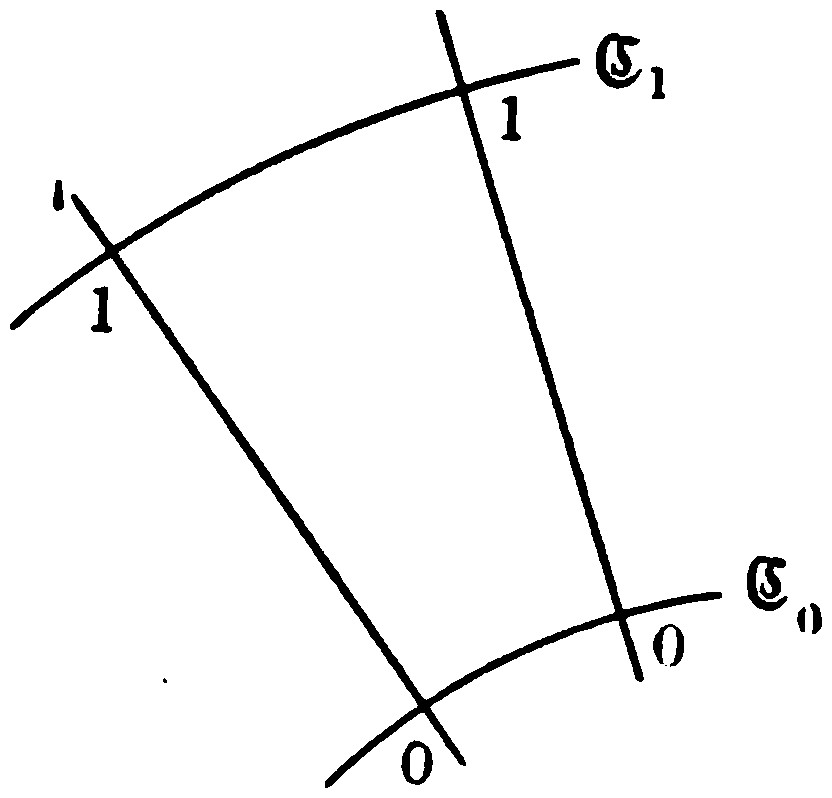
\includegraphics[width=\linewidth,height=32mm,keepaspectratio]{figures/fig01_src_clean_x8.png}
\end{minipage}\hfill
\begin{minipage}[c]{0.49\linewidth}\centering
\end{minipage}
\end{center}

因此，在横截曲线 $\mathfrak{C}_0$ 的场极值曲线上截取诸弧 01，使积分 $\overline{J}_{01}$ 具有相同数值，则点 1 的轨迹又是一条正则曲线，并被场的极值曲线横截。（参见图1；在该图以及后来大多数图中，极值曲线画成直线，横截位置用垂直相交来表示。）

% src-pdfpage=0071
% src-break=0071
所得结果显然是高斯著名定理的推广：一族等长测地线弧若垂直于含有其初始点的曲线，也垂直于其终点的轨迹；因为对测地线而言（第11节），横截位置与垂直位置重合。

\begin{center}{\large \S~16.}\end{center}

设被积函数 $F(x,y,x',y')$ 正则且不为零，例如为正；这一点或者 a) 对弧 $\mathfrak{B}$ 上一切与 $t$ 增大方向相应的弧元成立，或者 b) 对从该弧各点向任意方向出发的一切线元成立。只要充分限制场的范围，函数 $F$ 的这些性质在情形 a) 下对所有从场内各点出发、与弧 $\mathfrak{B}$ 上上述弧元倾斜得充分少的弧元仍成立，在情形 b) 下则对所有从场内各点出发的弧元仍成立。因为依第3节，对每个单独线元可取
\[
x'^2+y'^2=1,
\quad x'=\cos\varphi,
\quad y'=\sin\varphi;
\]
于是 $\varphi$ 是弧元相对于 $+x$ 轴、按正旋转方向（第4节）量出的倾角；若 $F(x,y,x',y')$ 在由 $x,y,\varphi$ 表征的线元上正则，则 $F$ 是 $x,y,\varphi$ 的正则函数。由此立即得到上述断言，因为一个函数若在某处正则，就在该处的某个邻域内保持此性质。

在较窄或较宽的任一假设下，
\[
\frac{\partial u}{\partial t}=F(\xi,\eta,\xi_t,\eta_t)
\]
在场内都不为零。因此，对于属于场的每一个值组 $(t,a)$，若曲线 $\mathfrak{C}_0$ 像以前一样被场的极值曲线横截，则可由方程
\[
u=\int_{t_0}^{t}F(\xi,\eta,\xi_t,\eta_t)dt
\]
把 $t$，从而也把 $x$、$y$，算作 $u$、$a$ 的正则函数；由于函数行列式
\[
\frac{\partial(t,a)}{\partial(u,a)}=1:\frac{\partial u}{\partial t}
\]
不为零，故下式也不为零：
% src-pdfpage=0072
% src-break=0072
\begin{equation}\tag{36}
\frac{\partial(x,y)}{\partial(u,a)}
=\frac{\partial(\xi,\eta)}{\partial(t,a)}\frac{\partial(t,a)}{\partial(u,a)}
=\Delta:\frac{\partial u}{\partial t}
=\frac{\Delta}{F(\xi,\eta,\xi_t,\eta_t)}.
\end{equation}
设想把用 $u$、$a$ 表出的 $x$、$y$ 代入函数 $F(x,y,dx,dy)$，并置
\[
v=a,
\quad \frac{dv}{du}=s,
\]
所得为
\[
F(x,y,dx,dy)=G(u,v,du,dv)=g(u,v,s)du,
\]
\[
J=\int G(u,v,u',v')dt;
\]
那么 $G$，以及依第5节在 $du$ 不消失时的 $g(u,v,s)$，都在与 $F$ 相同的线元上正则。

沿场的极值曲线有
\[
v=a=\text{const.},\quad s=0,
\]
而由于 $F$ 为正，$u$ 沿 $t$ 增大的方向增长；所以
\[
u=\int_0^1G(u,v,du,0)=\int_0^1g(u,v,0)du,
\]
其中函数 $g$ 按 $du$ 为正值来形成。对 $u$ 微分，并注意作为曲线 $\mathfrak{C}_0$ 与直线 $v=\text{const.}$ 之交点的 0 不依赖于 $u$，便得恒等式
\[
1=g(u,v,0),
\]
或当 $du>0$ 时，
\[
G(u,v,du,0)=du.
\]

把第15节所述每条直线 $u=\text{const.}$ 都被极值曲线 $v=\text{const.}$ 横截这一事实，用变量 $u,v$ 表示出来，还可得到关于函数 $g$ 的进一步规定。设值组
\[
x,y,x',y';\quad u,v,u',v'
\]
表示同一线元，其中导数对任意参数取得，则有恒等式
\[
F(x,y,x',y')=G(u,v,u',v'),
\]
\[
x'=x_u u'+x_v v',\quad y'=y_u u'+y_v v',
\]
\[
u'=u_xx'+u_yy',\quad v'=v_xx'+v_yy'.
\]
对第一个恒等式关于 $x'$、$y'$ 微分，得到
% src-pdfpage=0073
% src-break=0073
\[
F_{x'}=G_{u'}\frac{\partial u'}{\partial x'}+G_{v'}\frac{\partial v'}{\partial x'}
=u_xG_{u'}+v_xG_{v'},
\quad F_{y'}=u_yG_{u'}+v_yG_{v'}.
\]
另一方面，沿任意方向前进时有
\[
Dx=x_uDu+x_vDv,
\quad Dy=y_uDu+y_vDv,
\]
因而有恒等式
\[
F_{x'}Dx+F_{y'}Dy
=\{G_{u'}(u_xx_u+u_yy_u)+G_{v'}(v_xx_u+v_yy_u)\}Du+\cdots,
\]
又因为显然
\[
\frac{\partial u}{\partial u}=u_xx_u+u_yy_u=1,
\quad
\frac{\partial v}{\partial u}=v_xx_u+v_yy_u=0,
\]
以及另有两个相似方程，便得到恒等式
\[
F_{x'}Dx+F_{y'}Dy=G_{u'}Du+G_{v'}Dv.
\]
按照第15节，当 $D$ 表示沿曲线 $u=\text{const.}$ 前进，而导数取在场的极值曲线上时，这个量消失；所以方程
\[
G_{u'}Du+G_{v'}Dv=(g-sg_s)Du+g_sDv=0
\]
必须由 $s=0$、$Du=0$ 得到满足，从而
\[
g_s(u,v,0)=0.
\]
由所得的 $g(u,v,0)$ 值，函数 $g$ 的泰勒展开在 $\theta$ 属于从 0 到 $+1$ 的线段时取形式
\begin{equation}\tag{37}
g(u,v,s)=1+\frac{s^2}{2}g_{ss}(u,v,\theta s).
\end{equation}
在假设 a) 下，只要 $|s|$ 不超过某个正量，此方程成立；在假设 b) 下，它对 $s$ 的每个有限值成立。显然，当 $\mathfrak{C}_0$ 退化为一点时，以上推导仍然有效。

\begin{center}
{\small 图~2}\par\vspace{1mm}
\begin{minipage}[c]{0.47\linewidth}\centering
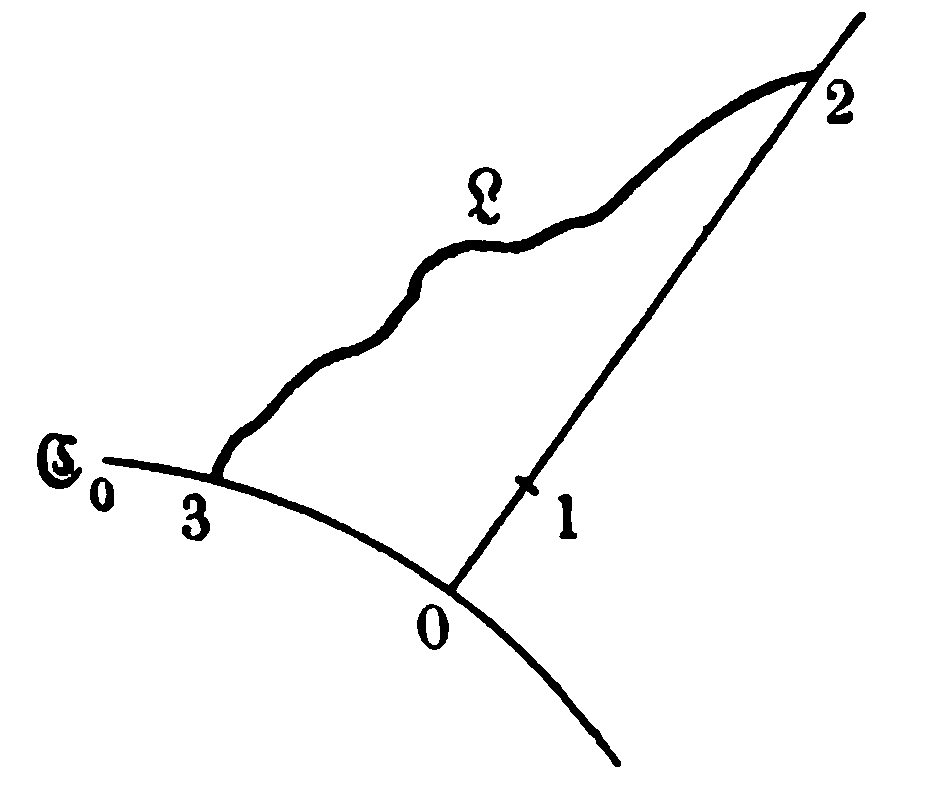
\includegraphics[width=\linewidth,height=32mm,keepaspectratio]{figures/fig02_src_clean_x8.png}
\end{minipage}\hfill
\begin{minipage}[c]{0.49\linewidth}\centering
\end{minipage}
\end{center}

现设（图2）12 是属于场的任意弧 $\mathfrak{B}$；如前，0 是包含该弧的极值曲线 $\mathfrak{E}$ 与 $\mathfrak{C}_0$ 的交点；3 是后一曲线上的一个固定点，并用曲线 $\Omega$ 与 2 相连。该曲线不离开场；沿此曲线，令 $x,y$ 是参数 $\tau$ 的函数，$\tau$ 沿积分方向增长，使积分
% src-pdfpage=0074
% src-break=0074
\[
J_{32}=\int_{\tau_3}^{\tau_2}F\left(x,y,\frac{dx}{d\tau},\frac{dy}{d\tau}\right)d\tau
=\int_{\tau_3}^{\tau_2}G\left(u,v,\frac{du}{d\tau},\frac{dv}{d\tau}\right)d\tau
\]
具有一个确定的有限值，并满足方程
\begin{equation}\tag{38}
\int_{\tau_3}^{\tau_2}\frac{du}{d\tau}d\tau
=\left.u\right|_3^2
=\left.u\right|_0^2
\end{equation}
那么显然
\begin{equation}\tag{39}
J_{32}-\overline{J}_{02}
=\int_3^2\left[G\left(u,v,\frac{du}{d\tau},\frac{dv}{d\tau}\right)-\frac{du}{d\tau}\right]d\tau;
\end{equation}
只要 $du/d\tau$ 为正，被积函数依 (37) 可写成
\begin{equation}\tag{40}
\frac{s^2}{2}g_{ss}(u,v,\theta s)\frac{du}{d\tau};
\end{equation}
若 $du/d\tau$ 为负或为零，则该被积函数与 $G$ 一样为正。

为了判定这个积分的符号，无须实际形成往往难以求得的函数 $g$；可以从 $x',y',u',v'$ 之间上述线性关系出发。两次应用这些关系，得到
\[
\frac{\partial^2G}{\partial v'^2}=G_{v'v'}=F_{x'x'}x_v^2+2F_{x'y'}x_vy_v+F_{y'y'}y_v^2.
\]
由恒等式
\[
F=x'F_{x'}+y'F_{y'}
\]
分别对 $x'$、$y'$ 微分，得
\[
x'F_{x'x'}+y'F_{x'y'}=x'F_{y'x'}+y'F_{y'y'}=0;
\]
注意 $x'$、$y'$ 不同时消失，便知诸量
\[
F_{x'x'}:y'^2,
\quad F_{y'y'}:x'^2
\]
中有一个具有有限值 $F_1(x,y,x',y')$，并满足
\[
F_{x'x'}=F_1y'^2,
\quad F_{x'y'}=-x'y'F_1,
\quad F_{y'y'}=x'^2F_1,
\quad F_1dt=\frac{f_{pp}dx}{x'^4}.
\]
把这些值代入 $G_{v'v'}$ 的表达式，得到
% src-pdfpage=0075
% src-break=0075
\[
G_{v'v'}=F_1(x_vy'-y_vx')^2,
\]
而由于
\[
G=u'g\left(u,v,\frac{v'}{u'}\right),
\]
当 $u'$ 不消失时便有
\[
\frac{g_{ss}(u,v,s)}{u'}=F_1(x_vy'-y_vx')^2,
\]
或者根据 $x',y'$ 与 $u',v'$ 之间的线性方程，
\[
\frac{g_{ss}(u,v,s)}{u'}=F_1\,(x_vy_u-x_uy_v)^2u'^2,
\]
而右端出现的括号依 (36) 不为零。

现对情形 a)、b) 都假定：恰在每一种情形中 $F$ 正则的那些线元上，$F_1$ 具有固定符号且不消失。与本节开头相同的考察表明，在情形 a) 只须对弧 $\mathfrak{B}$ 的弧元假定 $F_1$ 的这一性质，在情形 b) 只须对从其各点出发的弧元作此假定。沿该弧有 $s=0$；所以若沿曲线 $\Omega$ 的 $|s|$ 不超过某个常数，则在假设 a) 下，诸量
\[
g_{ss}(u,v,\theta s),
\quad \int\frac{s^2}{2}g_{ss}(u,v,\theta s)du
\]
与 $F_1$ 同号，且 $u'$ 始终为正；量
\begin{equation}\tag{41}
G\left(u,v,\frac{du}{d\tau},\frac{dv}{d\tau}\right)-\frac{du}{d\tau}
\end{equation}
始终可写成形式 (40)，也与 $F_1$ 同号。反之，只要 $du/d\tau$ 在某些地方不再为正，就引入假设 b)；此时对 $u'>0$ 有
\[
G(u,v,u',v')-u'=\frac{s^2}{2}g_{ss}(u,v,\theta s)u'
=\frac{v'^2}{2u'}g_{ss}(u,v,\theta s).
\]
% src-pdfpage=0076
% src-break=0076
因此，让线元 $(u,v,u',v')$ 绕一固定点旋转，并令 $u'$ 从正侧趋于零，则左端趋于极限 $G(u,v,0,v')$，而右端具有 $F_1$ 的符号；后者必与我们假定为正的被积函数 $G$ 或 $F$ 的符号一致，即 $F_1$ 也为正。量 (41) 在 $du/d\tau$ 为正时是正的，并且只有 $s=0$ 时才消失；当 $du/d\tau$ 为负或为零时，它显然也为正。所以，只要方程 (38) 正确而积分表示 (39) 有意义，差 $J_{32}-\overline{J}_{02}$ 也为正。

\begin{center}{\large \S~17.}\end{center}

极值的概念必须通过说明要拿来比较的所有曲线的总体而更精确地规定。极值的一般观念要求我们首先比较邻近曲线；对于邻近性，引入如下定义。设 12 是任一平面弧；若弧 $\Omega$ 完全位于这样一个面积区域内部：半径为常数 $\rho$ 的圆以圆心沿弧 12 移动所覆盖的区域，则称一切相应的 $\rho$ 不超过某个常数的曲线 $\Omega$ 属于弧 12 的较宽邻域。若还存在一个正的常数 $\rho_1$，使弧 $\Omega$ 的每条切线至少可与弧 12 的一条切线比较，而后者切点与前者切点的距离小于 $\rho$，并且两切线所成角小于 $\rho_1$，则只要 $\rho$、$\rho_1$ 保持在某些常数以下，称弧 $\Omega$ 位于弧 12 的较窄邻域内。这些定义显然可以立即推广到空间曲线。再者，若当 $\Omega$ 位于弧 12 的较宽邻域内时，沿两条弧形成的积分 $J$ 之差具有固定符号，则称弧 12 给出积分 $J$ 的强极值。反之，若只有当 $\Omega$ 位于 12 的较窄邻域内时，该差才具有固定符号，则称发生弱极值。显然，在后一情形中，用来与弧 12 比较的曲线 $\Omega$ 的区域比前一情形更窄。

不过，为了能够证明极值，我们必须对曲线 $\Omega$ 假定某些连续性性质，
% src-pdfpage=0077
% src-break=0077
其本质是：沿这些曲线可以形成形如 $J$ 的积分，并按微积分的通常运算规则处理。为了精确表述这些性质，一般地考察一个函数 $\varphi(\tau)$，它在任一有界区间 $\mathfrak{J}$ 内具有如下性质。它连续，并且商
\[
\frac{\varphi(\tau+\varepsilon)-\varphi(\tau)}{\varepsilon}
\]
在 $\varepsilon$ 为正且无限减小时，对每个 $\tau$ 值趋于某个确定的有限极限 $\varphi'(\tau)$。这里不必排除商
\[
\frac{\varphi(\tau-\varepsilon)-\varphi(\tau)}{-\varepsilon}
\]
趋于另一个极限，甚至根本不趋于任何极限。像有时所作的那样，我们称量 $\varphi'(\tau)$ 为右导数。对于它，正如通常的导数概念，也成立如下定理：若连续函数 $\varphi(\tau)$ 的右导数在从 $\tau_0$ 到 $\tau_1$ 的区间处处等于确定值零，则 $\varphi(\tau)$ 在该区间必为常数。事实上，令
\[
\psi(\tau)=\varphi(\tau)+\alpha(\tau-\tau_0),
\quad \theta(\tau)=\varphi(\tau)-\alpha(\tau-\tau_0),
\]
其中 $\alpha$ 为正常数，则 $\psi(\tau)$ 的右导数为 $\alpha$，$\theta(\tau)$ 的右导数为 $-\alpha$；所以前一函数在 $\tau_0$ 与 $\tau_1$ 之间递增，后一函数递减。若 $\tau_1>\tau_0$，就有不等式
\[
\psi(\tau_1)>\psi(\tau_0),
\quad \theta(\tau_1)<\theta(\tau_0),
\]
\[
\varphi(\tau_1)+\alpha(\tau_1-\tau_0)>\varphi(\tau_0),
\quad \varphi(\tau_1)-\alpha(\tau_1-\tau_0)<\varphi(\tau_0),
\]
\[
\alpha(\tau_1-\tau_0)>\varphi(\tau_0)-\varphi(\tau_1)>-\alpha(\tau_1-\tau_0).
\]
由于 $\alpha$ 可以任意小，最后一个不等式给出 $\varphi(\tau_1)=\varphi(\tau_0)$，断言得证。

除去这个特殊情形，现再假定函数 $\varphi'(\tau)$ 具有如下性质。它在任一区间内的振幅，定义为该区间内函数任意两个可取值之差的绝对值的上界；在区间 $\mathfrak{J}$ 内，凡 $\varphi'(\tau)$ 的振幅超过某个正常数的各部分，
% src-pdfpage=0078
% src-break=0078
其总长度总可以作成无限小。于是按黎曼，函数 $\varphi'(\tau)$ 可积，积分
\[
\Phi(\tau)=\int_{\tau_0}^{\tau}\varphi'(\tau)d\tau,
\]
其积分区间是 $\mathfrak{J}$ 的一部分，是 $\tau$ 的有限连续函数。再假定，当 $\varepsilon$ 为正时，
\[
\lim_{\varepsilon=0}\varphi'(\tau+\varepsilon)=\varphi'(\tau);
\]
这样以某种方式限制了函数 $\varphi'(\tau)$ 的不连续性，但例如仍可能在任一不连续点的任意邻域内存在无穷多个其他不连续点。在这个假设下，若量 $\varphi'(\tau)$ 在某一点为正，它就在沿某一有限区间上为正。又对 $\varepsilon>0$ 有
\[
\Phi(\tau+\varepsilon)-\Phi(\tau)
=\int_{\tau}^{\tau+\varepsilon}\varphi'(\tau)d\tau=M\varepsilon,
\]
其中 $M$ 位于 $\varphi'(\tau)$ 在 $\tau$ 与 $\tau+\varepsilon$ 之间所取值的上下界之间；由前一方程，$\varepsilon$ 消失时 $M$ 收敛于 $\varphi'(\tau)$。所以量 $\Phi(\tau)$ 具有右导数
\[
\Phi'(\tau)=\varphi'(\tau),
\]
差 $\Phi(\tau)-\varphi(\tau)$ 为常数；又因 $\Phi(\tau_0)$ 消失，便得到
\[
\Phi(\tau)=\varphi(\tau)-\varphi(\tau_0)=\int_{\tau_0}^{\tau}\varphi'(\tau)d\tau.
\]
因此，只要把微分运算理解为右导数，微分与积分之间通常的基本关系仍然成立。

现设 $x$、$y$ 沿曲线 $\Omega$ 是参数 $\tau$ 的函数，并具有函数 $\varphi(\tau)$ 的性质，即具有可积的右导数，我们仍用通常的微分符号表示它们；同时假定和
\[
\left(\frac{dx}{d\tau}\right)^2+
\left(\frac{dy}{d\tau}\right)^2
\]
始终大于某个正常数。因为 $\varphi'(\tau)$ 不必连续，这完全不排除曲线 $\Omega$
% src-pdfpage=0079
% src-break=0079
具有有限个或无穷多个角点；但它在每一点都有一个与 $\tau$ 增大方向相应的确定方向。若 $\Omega$ 位于弧 $\mathfrak{B}$ 的充分有限的较窄或较宽邻域内，分别对应于前节的假设 a) 或 b)，则在第一种情形，每一个值组
\[
\left(x,y,\frac{dx}{d\tau},\frac{dy}{d\tau}\right)
\]
都任意接近于一个表示曲线 $\mathfrak{E}$ 弧元的值组；在第二种情形，$F$ 对从场内各点向任意方向出发的线元正则。因此，在两种情形中，$F$ 对曲线 $\Omega$ 所定义的每个值组
\[
\left(x,y,\frac{dx}{d\tau},\frac{dy}{d\tau}\right)
\]
都正则，而对应于论元 $\tau$ 的可变区间的量
\[
F\left(x,y,\frac{dx}{d\tau},\frac{dy}{d\tau}\right)
\]
的振幅，随同一该区间内诸量
\[
\frac{dx}{d\tau},\quad \frac{dy}{d\tau}
\]
的振幅无限趋于零。再令
\[
F\left(x,y,\frac{dx}{d\tau},\frac{dy}{d\tau}\right)=\Theta(\tau),
\]
则因 $dx/d\tau$、$dy/d\tau$ 满足这样的方程，显然当 $\varepsilon>0$ 时，
\[
\Theta(\tau)=\lim_{\varepsilon=0}\Theta(\tau+\varepsilon).
\]
所以 $\Theta(\tau)$ 具有上面对 $\varphi'(\tau)$ 假定的一切性质，是可积的，并给出方程
\[
\frac{d}{d\tau}\int_{\tau_0}^{\tau}\Theta(\tau)d\tau
=\frac{d}{d\tau}\int_{\tau_0}^{\tau}F\left(x,y,\frac{dx}{d\tau},\frac{dy}{d\tau}\right)
=F\left(x,y,\frac{dx}{d\tau},\frac{dy}{d\tau}\right),
\]
这与积分学的通常规则一致。若 $\Phi(x,y)$ 是沿曲线 $\Omega$ 的坐标正则函数，则量
\[
\frac{d\Phi}{d\tau}=\Phi_x\frac{dx}{d\tau}+\Phi_y\frac{dy}{d\tau}
\]
也具有与 $F$ 相同的性质。把这些说明应用于作为坐标正则函数的量 $u,v$，便知诸量
% src-pdfpage=0080
% src-break=0080
\[
G\left(u,v,\frac{du}{d\tau},\frac{dv}{d\tau}\right),
\quad \frac{du}{d\tau},\quad \frac{dv}{d\tau}
\]
具有 $\varphi'(\tau)$ 的性质；特别地，若其中前两个量之差在一个点为正，就沿某一有限区间为正。又可知，在上述假设下方程 (38)、(39) 正确，只要把关于 $\tau$ 的微分符号总理解为右导数。形成 $J_{32}$ 时，这完全自然，因为积分沿 $\tau$ 增大的方向进行。

根据这些推导，现在可以严格证明量
\[
J_{32}-\overline{J}_{02}
=\int_3^2\left[G\left(u,v,\frac{du}{d\tau},\frac{dv}{d\tau}\right)-\frac{du}{d\tau}\right]d\tau
\]
与 $F_1$ 同号，并且只有当曲线 $\Omega$ 与 $\mathfrak{B}$ 完全重合时才消失。在情形 a) 下，这立即清楚，因为沿整个积分区间可把被积函数换成
\begin{equation}\tag{42}
\frac{s^2}{2}g_{ss}(u,v,\theta s)\frac{du}{d\tau}
\end{equation}
而量 $g_{ss}du$ 依假设不消失。在情形 b) 下，被积函数也从不为负；若 $J_{32}-\overline{J}_{02}$ 应消失，则至少在 $du/d\tau$ 为正的地方，量 $dv/d\tau$ 不得不为零，因为此时被积函数又可写成形式 (42)，因而为正。若 $du/d\tau$ 在某一点变为负，则上述积分的被积函数也为正；又因如上所述，它若在一点为正，就沿某一有限区间保持为正，所以积分 $J_{32}-\overline{J}_{02}$ 只有在 $v$ 沿曲线 $\Omega$ 为常数、从而后一曲线与 $\mathfrak{B}$ 重合时才可能消失。

这样，极值的证明完成了；无论把弧 02 与一切具有相同端点的弧相比，还是与一切从曲线 $\mathfrak{C}_0$ 通向点 2 的弧相比，结论都一样。不过，若曲线 $\mathfrak{C}_0$ 收缩为点 0，
% src-pdfpage=0081
% src-break=0081
从而场的所有极值曲线都通过该点，则还必须特别假定曲线 $\Omega$ 始终留在由场的极值曲线简单覆盖的区域内（图3）。例如，可令所有曲线 $\Omega$ 都与曲线 $\mathfrak{E}$ 共有一段任意小的定长曲线段 01（图4）；此时

\begin{center}
\begin{minipage}[c]{0.47\linewidth}\centering
{\small 图~3}\par\vspace{1mm}
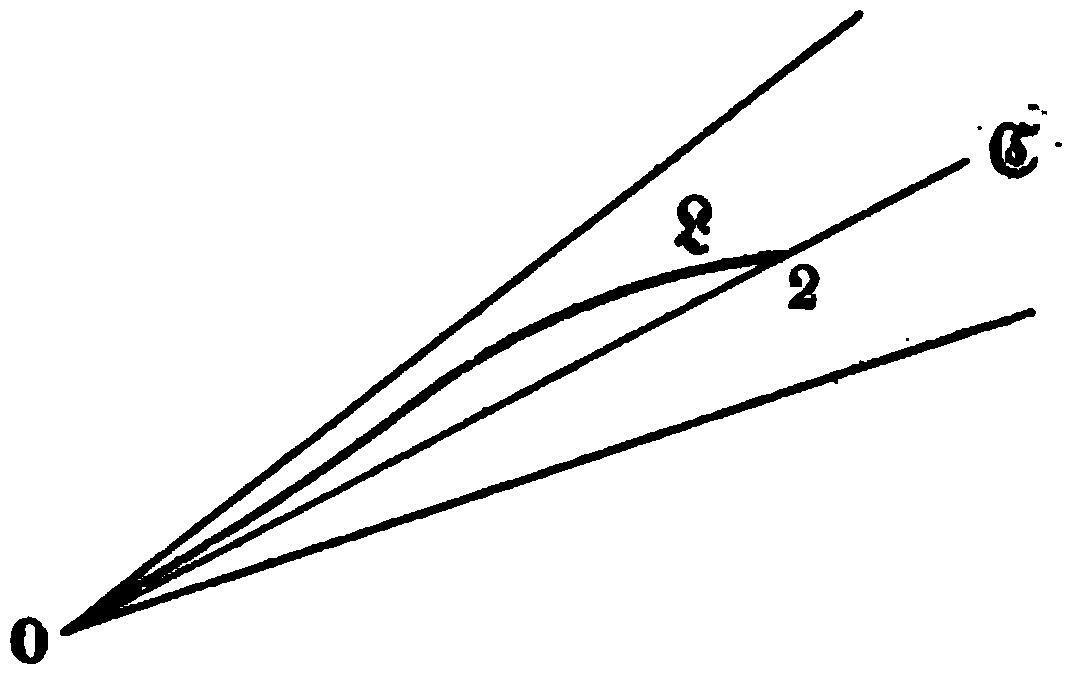
\includegraphics[width=\linewidth,height=24mm,keepaspectratio]{figures/fig03_src_clean_x8.png}\par\vspace{1mm}
\end{minipage}\hfill
\begin{minipage}[c]{0.47\linewidth}\centering
{\small 图~4}\par\vspace{1mm}
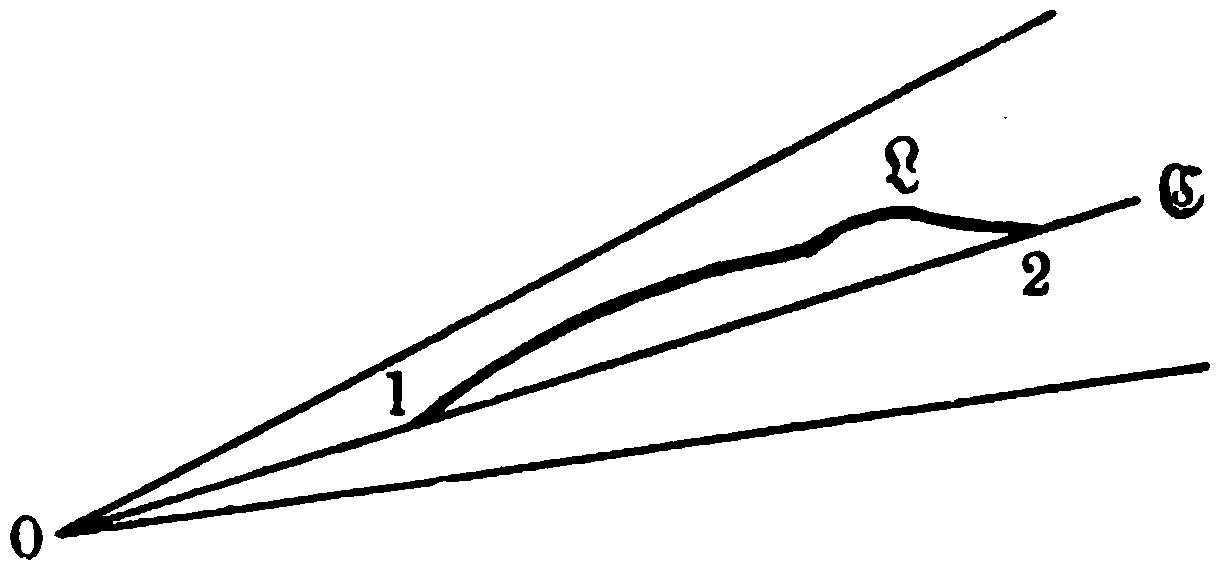
\includegraphics[width=\linewidth,height=24mm,keepaspectratio]{figures/fig04_src_clean_x8.png}\par\vspace{1mm}
\end{minipage}
\end{center}
\[
J_{32}-\overline{J}_{02}=J_{02}-\overline{J}_{02}=\overline{J}_{01}+J_{12}-\overline{J}_{02}=J_{12}-\overline{J}_{12},
\]
所以，对于弧 12，相对于所有具有相同端点的弧，极值在上述定义的不受限意义下得到保证。即使极值曲线在点 0 变为奇异，只要第15节为这种情形所述的假设成立，结论也成立。最后容易看出，若让点 2 作为弧 $\Omega$ 的端点，在一条被场的极值曲线横截的曲线 $\mathfrak{C}_2$ 上移动，而保持 0 不动，以致积分方向与此前假设相反，从固定点通向固定曲线，上述论证也不改变。

我们在第16节限制了曲线 $\Omega$ 所在场的范围，以便把点或曲线 $\mathfrak{E}$ 弧元上的假设 a)、b) 推广到场的一切极值曲线；在第15节也限制了场，使曲线 $u=\text{const.}$ 保持正则且每条只与场的每条极值曲线相交一次。如果在一个特殊问题中，对于一个有有限范围的确定场，可以证明这些总能通过限制场而获得的性质，则我们的论证适用于该场内运行的每条曲线 $\Omega$，所得内容还多于极值的证明；因为只要构造出一个范围任意小的场，极值本身就已得到保证。

% src-pdfpage=0082
% src-break=0082
把所得最重要的结果概括如下。1. 雅可比条件：端点为 0、2 的一段处处非奇异的极值曲线被一个场包围。2. 勒让德条件：或者 a) 对沿 0 到 2 的方向走遍的弧 02 的所有弧元，或者 b) 对从该弧各点出发的一切线元，量 $F_1$ 或 $f_{pp}dx$ 具有固定符号且不消失，并且 $F$ 正则而不为零。那么弧 02 给出积分 $J$ 的一个极值；无论同一切具有相同端点的曲线 $\Omega$ 比较，还是同一切把从点 0 出发并被场的极值曲线横截的曲线 $\mathfrak{C}_0$ 与点 2 相连的曲线比较，都是如此。分别在假设 b) 或 a) 下，强极值或弱极值得到保证；分别在 $F_1$ 为负或为正时，出现最大值或最小值。

% src-pdfpage=0082
% src-break=0082
\begin{center}{\large \S~18.}\end{center}

\noindent\textbf{例。问题一（第9节）。} 这里有
\[
Fdt=\sqrt{x'^2+y'^2}\,dt,
\]
平方根取正，因而
\[
y'^2F_1=F_{x'x'}=\frac{\partial}{\partial x'}
\left(\frac{x'}{\sqrt{x'^2+y'^2}}\right)
=\frac{y'^2}{\left(\sqrt{x'^2+y'^2}\right)^3},
\]
\[
F_1=\left(\frac{1}{\sqrt{x'^2+y'^2}}\right)^3,
\]
其中平方根同样取正。又有
\[
Fdt=f\,dx,\quad f=\sqrt{1+p^2},\quad
f_{pp}=\left(\frac{1}{\sqrt{1+p^2}}\right)^3,
\]
其中平方根具有 $dx$ 的符号，所以每一弧元上的 $f_{pp}dx$ 与 $F_1$ 一样为正。因此，强最小值的勒让德符号条件得到满足。

为研究直线段 12 是否给出 1 与 2 之间的最短线，设（图5）$\Omega$ 是第17节所述连续性性质的任一条从 1 到 2 的线，并给出弧积分 $J_{12}$；
% src-pdfpage=0083
% src-break=0083
线段 12 的长度为 $\overline{J}_{12}$。再设 0 是直线 12 上不属于曲线 $\Omega$ 且位于线段 12 外的一个点；以它为直角坐标和极坐标的原点，置
\[
x=t\cos v,\quad y=t\sin v,
\]
并选择常数 $\alpha,\beta$，使
\[
0<\alpha<\beta
\]
且曲线 $\Omega$ 完全位于圆 $t=\alpha$ 与 $t=\beta$ 之间的环形区域内部。该区域被极值曲线 $v=\text{const.}$ 恰好简单覆盖，并可视为直线段 12 的一个场，因为其中的量
\[
\frac{\partial(x,y)}{\partial(t,v)}
=
\begin{vmatrix}
\cos v & \sin v\\
-t\sin v & t\cos v
\end{vmatrix}
=t
\]
不为零。

\begin{center}
{\small 图~5}\par\vspace{1mm}
\begin{minipage}[c]{0.47\linewidth}\centering
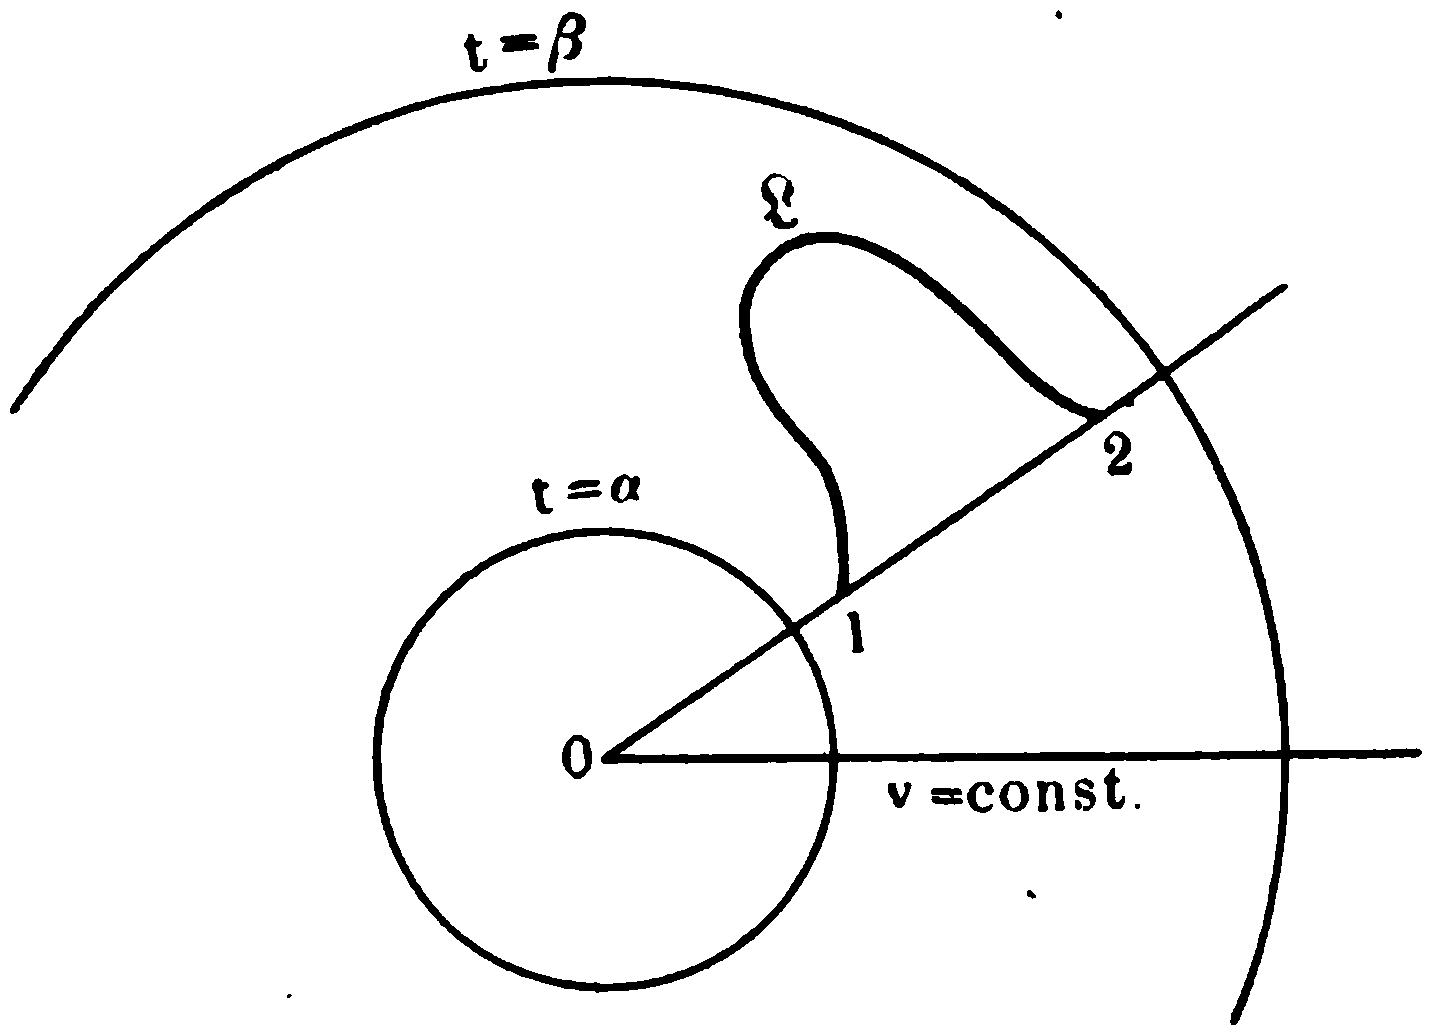
\includegraphics[width=\linewidth,height=32mm,keepaspectratio]{figures/fig05_src_clean_x8.png}
\end{minipage}\hfill
\begin{minipage}[c]{0.49\linewidth}\centering
\end{minipage}
\end{center}

一般理论中的曲线 $\mathfrak{C}_0$ 对应于圆 $t=\text{const.}$，每个圆与场的每条极值曲线各交于一点；$u$ 是从圆 $t=\alpha$ 起量出的直线 $v=\text{const.}$ 的长度，故
\[
u+\alpha=t,\quad
Fdt=\sqrt{dt^2+t^2dv^2}=\sqrt{du^2+(u+\alpha)^2dv^2}
=G(u,v,du,dv),
\]
\[
g(u,v,s)=\sqrt{1+(u+\alpha)^2s^2},
\]
最后一个平方根也取正，因为表达式 $g$ 只对 $du>0$ 的情形形成。在差
\[
J_{12}-\overline{J}_{12}
=
\int_{\tau_1}^{\tau_2}
\left[
G\left(u,v,\frac{du}{d\tau},\frac{dv}{d\tau}\right)
-\frac{du}{d\tau}
\right]d\tau
\]
中，只要 $\frac{du}{d\tau}$ 为负或消失，被积函数自然为正；这正表征曲线 $\Omega$ 上半径 $t$ 减小的那些部分。若 $\frac{du}{d\tau}$ 为正，被积函数可写成
% src-pdfpage=0084
% src-break=0084
\[
\sqrt{1+(u+\alpha)^2s^2}-1,
\]
所以也不为负，并且只有在 $s=0$ 时才消失。若 $s$ 在任何位置不为零，或被积函数为正，则依第17节，在曲线 $\Omega$ 的某一有限区间上也如此；因此差 $J_{12}-\overline{J}_{12}$ 只有在 $du$ 处处为正且 $s=0$ 时才可能消失。除去这种情形，显然有
\[
J_{12}>\overline{J}_{12},
\]
这就证明了强最小值，而且还得到更多。

进一步，设 $\mathfrak{C}_1$ 是由点 1 走遍的任一曲线，使 $x_1,y_1$ 是参数 $v$ 的正则函数；$n$ 是相对于 $v$ 增大方向，像 $+y$ 轴相对于 $+x$ 轴那样放置的法线方向。若置
\[
x=\xi(t,v)=x_1+t\cos(nx),\quad
y=\eta(t,v)=y_1+t\cos(ny),
\]
则 $v=\text{const.}$ 是曲线 $\mathfrak{C}_1$ 的一条法线，并且
\[
\Delta=\frac{\partial(\xi,\eta)}{\partial(t,v)}
=
\begin{vmatrix}
\cos(nx) & \dfrac{dx_1}{dv}+t\,\dfrac{d\cos(nx)}{dv}\\[1.1em]
\cos(ny) & \dfrac{dy_1}{dv}+t\,\dfrac{d\cos(ny)}{dv}
\end{vmatrix}.
\]
特别地，若 $v$ 是曲线 $\mathfrak{C}_1$ 上的弧长，则
\[
\cos(nx)=-\frac{dy_1}{dv},\quad \cos(ny)=\frac{dx_1}{dv},
\]
\[
\Delta=-1+t\left(
\frac{dx_1}{dv}\frac{d^2y_1}{dv^2}
-\frac{dy_1}{dv}\frac{d^2x_1}{dv^2}
\right)
=-1+\frac{t}{r},
\]
其中 $r$ 表示点 1 处的曲率半径；当曲率中心位于方向 $n$ 或相反方向时，分别取正或负。

现设在某条法线 $v=\text{const.}$ 上，从 1 指向点 2 的方向与 $n$ 一致，从而 $t_2$ 为正；那么，当 $r$ 为负，或者不等式
\[
0<t_2<r
\]
成立时，长度为 $t_2$ 的直线段 12 可以被一个 $\Delta$ 不消失的场包围；也就是说，只要线段 12 不包含点 1 的曲率中心即可（图6）。该场的极值曲线
% src-pdfpage=0085
% src-break=0085
是法线 $v=\text{const.}$，它们横截曲线 $\mathfrak{C}_1$。因此一般理论表明，直线段 12 给出曲线 $\mathfrak{C}_1$ 与点 2 之间距离的一个强最小值，并且短于场内任何具有上述连续性性质、从曲线 $\mathfrak{C}_1$ 通向点 2 的线 $\Omega$。量 $u$ 是到曲线 $\mathfrak{C}_1$ 的法向距离；容易得到公式

\begin{center}
{\small 图~6}\par\vspace{1mm}
\begin{minipage}[c]{0.47\linewidth}\centering
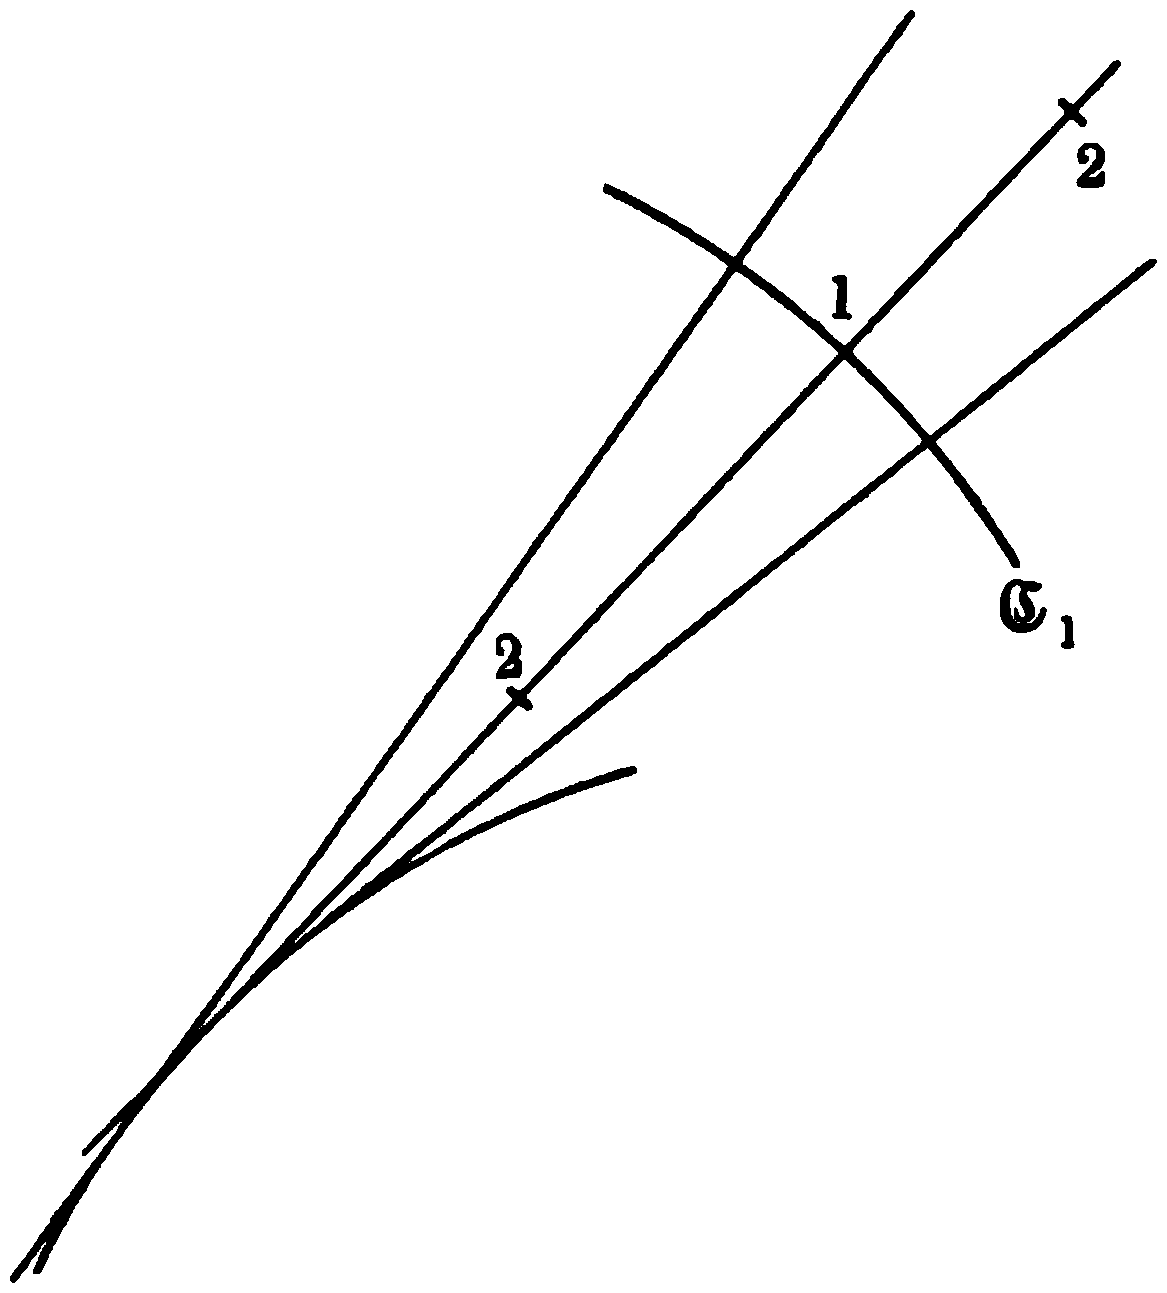
\includegraphics[width=\linewidth,height=32mm,keepaspectratio]{figures/fig06_src_clean_x8.png}
\end{minipage}\hfill
\begin{minipage}[c]{0.49\linewidth}\centering
\end{minipage}
\end{center}

\[
\sqrt{dx^2+dy^2}
=
\sqrt{du^2+(u-r)^2dv^2}
=G(u,v,du,dv),
\]
由此可以作出与先前变换弧元时相同的推论。

\bigskip

\noindent\textbf{问题三（第9节）。} 设在 $wy$ 平面内，$\Omega$ 是从点 0 在半平面 $y>0$ 中引向 $w$ 轴的任一条长度为 $l$ 的线；沿该线，$w,y$ 作为参数 $\tau$ 的函数，具有第17节中 $\varphi(\tau)$ 的性质。要证明其面积积分小于长度为 $l$ 的半圆面积。若 $\frac{dw}{d\tau}$ 在某些区间为负，则考察由方程
\[
y=\int_{\tau_0}^{\tau}\frac{dy}{d\tau}\,d\tau,
\quad
w=\int_{\tau_0}^{\tau}\left|\frac{dw}{d\tau}\right|\,d\tau
\]
定义的曲线 $\Omega^0$；让 $\tau$ 取遍与曲线 $\Omega$ 上相同的区间，这条曲线也具有长度 $l$ 和相同的连续性性质，因为容易看出 $|\varphi(\tau)|$ 也具有第17节对 $\varphi(\tau)$ 所要求的性质。曲线 $\Omega^0$ 的面积积分有限，且只含正的弧元；显然有
% src-pdfpage=0086
% src-break=0086
\[
\int_{\tau_0}^{\tau}y\left|\frac{dw}{d\tau}\right|\,d\tau
\geqq
\int_{\tau_0}^{\tau}y\frac{dw}{d\tau}\,d\tau,
\]
即曲线 $\Omega^0$ 与 $w$ 轴所围的面积不小于曲线 $\Omega$ 所围的面积。因此只须证明前者小于上述半圆面积；此时我们获得的好处是，在积分
\[
J=\int y\sqrt{1-p^2}\,dx=\int y\,dw
\]
中平方根始终取正。曲线 $\Omega^0$ 在 $xy$ 平面中对应于一条曲线 $\Omega_0$；沿它，因为 $x$ 是曲线 $\Omega^0$ 的弧长，处处有
\begin{equation}\tag{43}
\frac{dx}{d\tau}>0,\quad -1\leqq\frac{dy}{dx}\leqq +1;\quad x>0,\quad 0\leqq y\leqq x;
\end{equation}
所以在 $xy$ 平面中根本不必证明强极值，只须把由这些不等式表征的曲线拿来比较。在所考察的一切曲线 $\Omega_0$ 上，最大值的勒让德条件得到满足，因为对这些曲线，量

\begin{center}
\begin{minipage}[c]{0.47\linewidth}\centering
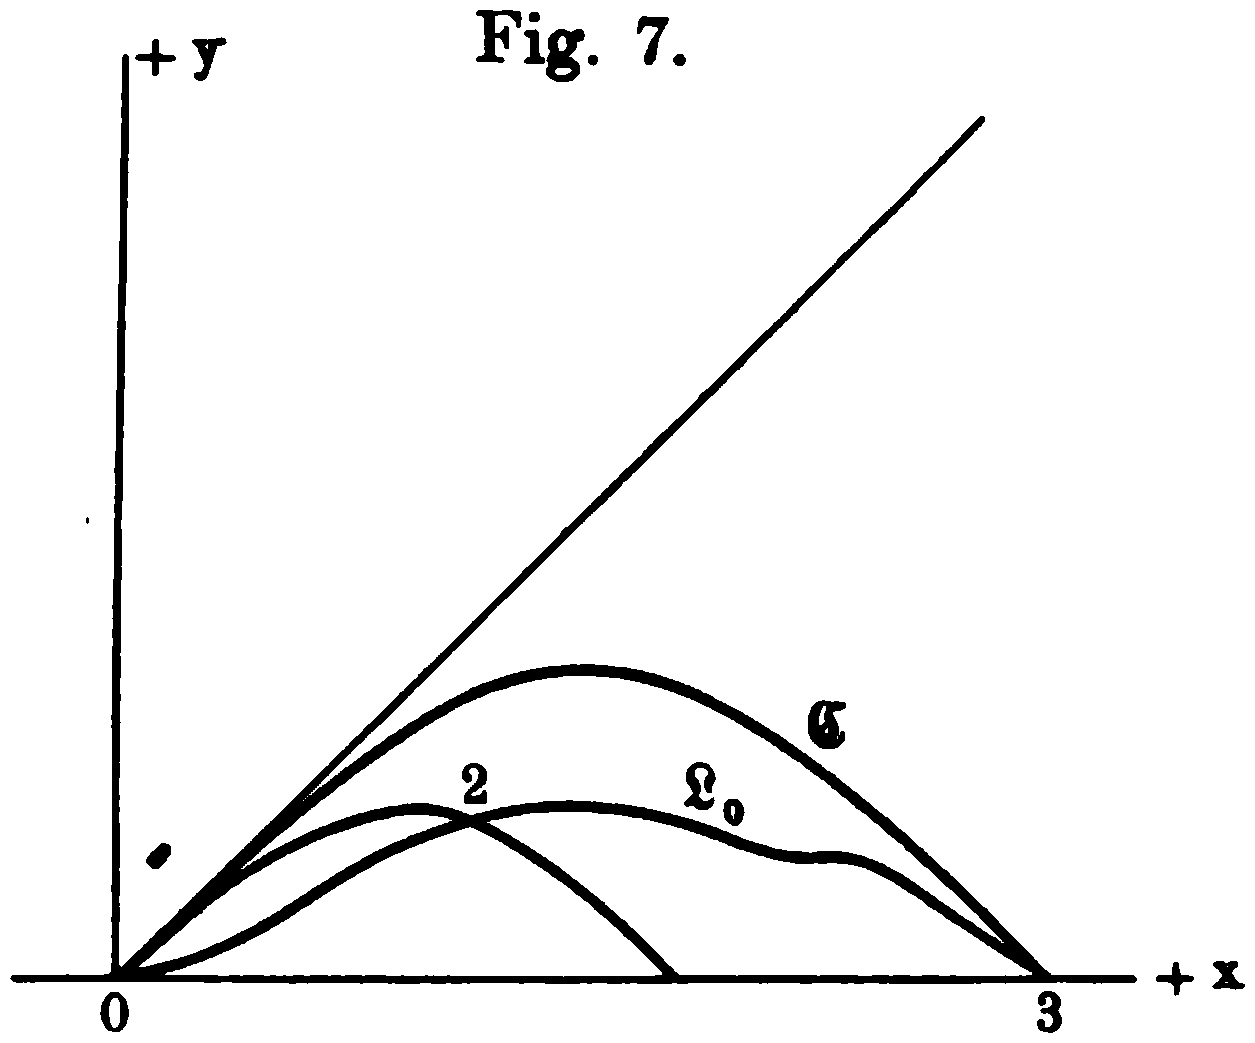
\includegraphics[width=\linewidth,height=32mm,keepaspectratio]{figures/fig07_src_clean_x8.png}
\end{minipage}\hfill
\begin{minipage}[c]{0.49\linewidth}\centering
\end{minipage}
\end{center}

\[
f_{pp}\,dx=\frac{-y\,dx}{\left(\sqrt{1-p^2}\right)^3}
\]
为负。

$xy$ 平面中由最后几个不等式 (43) 确定、曲线 $\Omega_0$ 位于其中并在图7中画出的八分区，被极值曲线
\[
y=a\sin\frac{x}{a},\quad a>0,\quad p=\cos\frac{x}{a},
\]
恰好简单覆盖；在每条极值曲线上取
\begin{equation}\tag{44}
0\leqq\frac{x}{a}\leqq\pi
\end{equation}
事实上，固定 $x$，则
\[
\frac{\partial y}{\partial a}
=\sin\frac{x}{a}-\frac{x}{a}\cos\frac{x}{a}
\]
% src-pdfpage=0087
% src-break=0087
因 $x$ 满足不等式 (44) 而始终为正。当 $a=0$ 时有 $y=0$，当 $a=\infty$ 时则有 $y=x$；所以当 $a$ 取遍所有正值时，点 $(x,y)$ 取遍属于该八分区、位于直线 $x=\text{const.}$ 上的一切点，而且每点只取一次。还可以令 $x=t$，于是
\[
\Delta=\frac{\partial(x,y)}{\partial(t,a)}
=\frac{\partial y}{\partial a},
\]
这个量如上所述为正，只要 $y$ 不消失也不出现条件 $=x$。设点 0、3 分别对应于 $x=0$ 和 $x=a\pi$；则极值曲线弧 03 不含任一端点的每一部分都可被一个场包围。端点本身则因其中 $p=\pm1$、函数 $F$ 变为奇异而需要特别考察。

按照一般理论，在曲线 $\mathfrak{C}_0$ 收缩为点 0 时，令
\[
u=\int_0^x y\sqrt{1-p^2}\,dx
=a\int_0^x\sin^2\frac{x}{a}\,dx
=\frac{ax}{2}-\frac{a^2}{2}\sin\frac{x}{a}\cos\frac{x}{a},
\]
其中平方根取正。利用表达式
\[
F=y\sqrt{x'^2-y'^2},\quad
F_{x'}=\frac{yx'}{\sqrt{x'^2-y'^2}},\quad
F_{y'}=-\frac{yy'}{\sqrt{x'^2-y'^2}},
\]
容易验证方程
\[
\frac{\partial u}{\partial a}
=
F_{x'}\frac{\partial x}{\partial a}
+
F_{y'}\frac{\partial y}{\partial a},
\quad
du=F_{x'}\,dx+F_{y'}\,dy.
\]
在 0 与 3 之间的任何曲线 $\Omega_0$ 上，这个微分 $du$ 都不能消失或变为负。事实上，若 $d$ 指沿曲线 $\Omega_0$ 前进，而 $x',y',p$ 则取在场的极值曲线上，那么由于 $dx$ 为正，并且对极值曲线取 $x=t$，从而可以把 $F_{x'}$ 看成正的，就会得到
\[
F_{x'}+F_{y'}\frac{dy}{dx}\leqq0,\quad
1+\frac{F_{y'}}{F_{x'}}\frac{dy}{dx}\leqq0,\quad
p\frac{dy}{dx}\geqq1.
\]
按第二个不等式 (43) 以及上面给出的 $p$ 值，这只有在 $p=\pm1$，也就是在 $x$ 轴上的点，才可能发生。因此量 $du:d\tau$ 在
% src-pdfpage=0088
% src-break=0088
点 0 与 3 之间始终为正，从而处处可以写成
\[
dJ_{02}=du\left[1+\frac{s^2}{2}\,g_{ss}(u,v,\theta s)\right],
\]
由上面已经确定的表达式 $f_{pp}dx$ 的性质，得到
\[
\frac{d(J_{02}-u)}{d\tau}<0.
\]

当
\[
dw=0,\quad dx=\pm dy
\]
时，微分 $dJ_{02}$ 向变量 $u,v$ 的变换变得不可能，因为此时被积函数 $F$ 奇异。尽管如此，原始定义
\[
J=\int y\,\frac{dw}{d\tau}\,d\tau
\]
表明，在这些位置 $J_{02}$ 仍然是第17节意义下的一个函数 $\varphi(\tau)$。显然，此时 $dJ_{02}:d\tau$ 消失，而对于 $du$ 有
\[
du=dx(F_{x'}\pm F_{y'})=a\,dx\left(1\pm\cos\frac{x}{a}\right),
\]
所以 $d(u-J_{02})$ 现在仍为正。因而，当点 2 沿曲线 $\Omega_0$ 从 0 走向 3 时，量 $u-J_{02}$ 增长。

由于点 0 的奇异性，$u$ 的初始值需要更仔细的研究。若不等式
\[
\left(\frac{dy}{d\tau}:\frac{dx}{d\tau}\right)^0<1
\]
成立，它首先显然为零；因为此时量 $a$ 只有在 $x=y$ 时才变为无穷，所以沿曲线 $\Omega_0$ 接近点 0 时保持在一个有限界以下，而 $u$ 的表达式立即表明 $u$ 与 $x$ 一同趋于极限零。反之，若有方程
\[
\left(\frac{dy}{d\tau}:\frac{dx}{d\tau}\right)^0=1,\quad
\lim_{\tau=\tau_0}\frac{y}{x}=1,
\]
则规定 $a$ 的方程，也就是说在置
\[
\varphi(z)=\frac{\sin z-z}{z}
\]
% src-pdfpage=0089
% src-break=0089
以后，方程
\[
\frac{y}{x}=1+\varphi\left(\frac{x}{a}\right)
\]
表明必有
\[
\left.\varphi\left(\frac{x}{a}\right)\right|^0=0.
\]
当 $z$ 位于 0 与 $\pi$ 之间时，量 $\varphi(z)$ 为负；又因不等式 (44) 成立，故
\[
\varphi\left(\frac{x}{a}\right)
\]
只有在
\[
\frac{x}{a}=0
\]
时才消失，从而此方程对点 0 得证。即使曲线 $\Omega_0$ 与直线 $y=x$ 共有一个有限曲线段，而 0 表示直线与曲线分开的那个点，结论显然也成立。把所得的 $\frac{x}{a}$ 值代入方程
\[
u=\frac{a^2}{4}\left\{\frac{2x}{a}-\sin\frac{2x}{a}\right\}
=
\frac{1}{4}\left\{
\frac{(2x)^2}{3!}\cdot\frac{2x}{a}
-
\frac{(2x)^2}{5!}\left(\frac{2x}{a}\right)^3
+\cdots
\right\},
\]
便看出在这种情形中，量 $u$ 作为 $\tau$ 的函数也在位置 0 从数值 0 开始。由于 $J_{02}$ 显然同样如此，便有
\[
\left.u-J_{02}\right|_{\tau_0}=0.
\]
所以差 $u-J_{02}$ 因为增长，在点 2 沿弧 $\Omega_0$ 行进而离开直线 $y=x$ 后立即为正；极限值
\[
\left.u\right|^3-J_{03}=\overline{J}_{03}-J_{03}
\]
同样为正。因此，曲线 $\Omega$ 和 $\Omega^0$ 同 $w$ 轴所围的面积，小于同样长度的半圆面积。

由所得结果可立即推出：一条闭曲线所围的面积，总小于同样长度的圆所围的面积；只要能用曲线上两个点 1、2 把该曲线分成两个等长部分，而直线段 12 完全位于内部，就可把该线段与 $w$ 轴等同。

\bigskip

\noindent\textbf{问题六（第11节）。} 任何不含尖点的极值曲线段都可被一个场包围；
% src-pdfpage=0090
% src-break=0090
例如在方程 (17) 中令量 $a$ 为常数，而只变动 $b$。此时场的极值曲线由一条曲线沿平行于 $x$ 轴的方向平移而得到；所以令 $t=p$，有
\[
\frac{\partial x}{\partial b}=1,\quad
\frac{\partial y}{\partial b}=0,\quad
\Delta=-\frac{dy}{dp},
\]
依 (18)，$\Delta$ 只有在尖点处才可能消失。又求得
\[
f_{pp}\,dx=-\frac{2yp(p^2-3)}{(1+p^2)^3}\,dx.
\]
这个量在方向相反的弧元上也取相反的值，因为这里属于第3节的第一种情形。所以强极值的勒让德符号条件不满足；但弱极值的条件满足，因为 $p^2-3$ 只在尖点改变符号。因此，不含尖点的一段极值曲线分别依其属于被尖点分开的两半中的一半或另一半，而给出弱最大值或弱最小值。当 $p^2<3$ 时，所求最小值存在。

\bigskip

\noindent\textbf{问题七（第11节）。} 引入新变量 $u,v$ 后，有形如
\[
\sqrt{E\,d\varphi^2+2F\,d\varphi\,d\psi+G\,d\psi^2}
=
\sqrt{E^0\,du^2+2F^0\,du\,dv+G^0\,dv^2}
=
du\sqrt{E^0+2F^0s+G^0s^2}
\]
的变换；方程
\[
g(u,v,0)=1,\quad g_s(u,v,0)=0
\]
因而给出
\[
E^0=1,\quad F^0=0.
\]
由 $E,E^0,F,\ldots$ 与直角坐标关于 $\varphi,\psi,u,v$ 的导数之间的联系，得到方程
\[
E^0G^0-F^0F^0=(EG-F^2)\left(\frac{\partial(\varphi,\psi)}{\partial(u,v)}\right)^2,
\]
或者若置
\[
G^0=m^2,
\]
则
\[
\Delta=\frac{\partial(\varphi,\psi)}{\partial(u,v)}
=\frac{m}{\sqrt{EG-F^2}}.
\]
% src-pdfpage=0091
% src-break=0091
所以，第17节所考察的被积函数特殊形式，正是线元的高斯形式
\[
\sqrt{du^2+m^2dv^2};
\]
垂直于一条给定曲线的测地线，在其中任一条的邻域内构成一个场，只要 $m$ 有限且不为零。

强最小值的勒让德条件得到满足，因为在第11节的记号下，
\[
\frac{\partial^2\Phi}{\partial\varphi'^2}
=
\frac{E}{\Phi}
-
\frac{(E\varphi'+F\psi')^2}{\Phi^3}
=
\frac{EG-F^2}{\Phi^3}\,\psi'^2,
\]
而这个量始终为正。

\begin{center}{\large \S~19.}\end{center}

关于 $u$ 的方程
\[
\frac{\partial u}{\partial x}=F_{x'},\quad
\frac{\partial u}{\partial y}=F_{y'}
\]
的右端只依赖于比 $y':x'$；消去这个比，得到 $u$ 的一个一阶偏微分方程，我们称之为雅可比—哈密顿方程。若 $U$ 是它的任一解，则可在方程
\begin{equation}\tag{45}
\frac{\partial U}{\partial x}=F_{x'},\quad
\frac{\partial U}{\partial y}=F_{y'},
\end{equation}
中取第一个方程，用来规定 $y':x'$ 的值；第二个方程便自动满足。把 $U$ 看作已知时，第一个方程可以视为 $x$、$y$ 之间的常微分方程，设其积分为
\begin{equation}\tag{46}
\varphi(x,y,a)=0
\end{equation}
并由一族单参数曲线 $\Omega$ 表示。若 $D$ 表示沿曲线 $U=\text{const.}$ 前进，则有
\[
\frac{\partial U}{\partial x}Dx+\frac{\partial U}{\partial y}Dy=0,\quad
F_{x'}Dx+F_{y'}Dy=0;
\]
所以曲线 $\Omega$ 相对于曲线 $U=\text{const.}$ 横截。再沿一条确定的曲线 $\Omega$，把任一函数
\begin{equation}\tag{47}
t=\psi(x,y)
\end{equation}
% src-pdfpage=0092
% src-break=0092
的值引入为参数，由其数值规定 $x$、$y$，则
\[
x'=\frac{\partial x}{\partial t},\quad y'=\frac{\partial y}{\partial t},
\]
其中应理解为从方程 (46)、(47) 把 $x$、$y$ 算作 $a$、$t$ 的函数。显然，也可以根据这些方程把 $t$、$a$，从而把 $x'$、$y'$，看作 $x$、$y$ 的函数；下文令符号 $\partial$ 指这种看法，而用下标表示导数仍保留原有意义，于是有方程
\begin{equation}\tag{48}
\frac{\partial F_{x'}}{\partial y}=\frac{\partial F_{y'}}{\partial x},
\end{equation}
\begin{equation}\tag{49}
\begin{aligned}
\frac{\partial F_{x'}}{\partial x}
&=
F_{x'x}+F_{x'x'}\frac{\partial x'}{\partial x}
+F_{x'y'}\frac{\partial y'}{\partial x},\\
\frac{\partial F_{y'}}{\partial x}
&=
F_{y'x}+F_{y'x'}\frac{\partial x'}{\partial x}
+F_{y'y'}\frac{\partial y'}{\partial x}.
\end{aligned}
\end{equation}
又如第16节所述，由函数 $F_{x'}$、$F_{y'}$ 的齐次性得到
\begin{equation}\tag{50}
F_{x'x'}x'+F_{x'y'}y'=0,\quad
F_{y'x'}x'+F_{y'y'}y'=0,
\end{equation}
根据方程 (49)，以及其中改为对 $y$ 微分的相似方程，由此有
\[
x'\frac{\partial F_{x'}}{\partial x}
+y'\frac{\partial F_{y'}}{\partial x}
=
x'F_{x'x}+y'F_{y'x}=F_x,
\]
\[
x'\frac{\partial F_{x'}}{\partial y}
+y'\frac{\partial F_{y'}}{\partial y}=F_y.
\]
但依方程 (48)，最后两个方程也可写成
\[
F_x=
\frac{\partial F_{x'}}{\partial x}x'
+\frac{\partial F_{x'}}{\partial y}y'
=\frac{dF_{x'}}{dt},
\]
\[
F_y=
\frac{\partial F_{y'}}{\partial x}x'
+\frac{\partial F_{y'}}{\partial y}y'
=\frac{dF_{y'}}{dt},
\]
由此可见，曲线 $\Omega$ 是积分 $J$ 的极值曲线。因此，若 $V$ 是从方程 (45) 消去 $x':y'$ 所得偏微分方程的任一解，则曲线 $V=\text{const.}$ 被积分 $J$ 的一族极值曲线横截。又显然，沿一条曲线 $\Omega$ 前进时，
% src-pdfpage=0093
% src-break=0093
\[
dV=(F_{x'}x'+F_{y'}y')\,dt=Fdt,
\]
所以可置
\[
V=\int Fdt,
\]
其中沿该族的一条极值曲线积分。

若函数 $V$ 含一个常数 $c$，则雅可比—哈密顿方程说明，可以把 $p$ 规定为 $x$、$c$ 的函数，使恒等式 (45) 成立。对这些恒等式关于 $c$ 微分，得到
\[
\frac{\partial^2 V}{\partial x\,\partial c}
=
\frac{\partial F_{x'}}{\partial p}\frac{\partial p}{\partial c},\quad
\frac{\partial^2 V}{\partial y\,\partial c}
=
\frac{\partial F_{y'}}{\partial p}\frac{\partial p}{\partial c}.
\]
现可置
\[
F_{x'}=\psi\left(\frac{y'}{x'}\right)=\psi(p),
\]
因而
\[
F_{x'y'}=\frac{1}{x'}\psi'(p)=\frac{1}{x'}\frac{\partial F_{x'}}{\partial p};
\]
对 $F_{y'}$ 也有相似结果。故
\[
\frac{\partial^2 V}{\partial x\,\partial c}
=
x'F_{x'y'}\frac{\partial p}{\partial c},\quad
\frac{\partial^2 V}{\partial y\,\partial c}
=
x'F_{y'y'}\frac{\partial p}{\partial c},
\]
而由方程 (50)，
\[
x'\frac{\partial^2V}{\partial x\,\partial c}
+
y'\frac{\partial^2V}{\partial y\,\partial c}=0.
\]
所以沿每一条曲线 $\Omega$，都有一个方程
\[
\frac{\partial V}{\partial c}=b.
\]
若其左端不是常数，这个方程便表示极值曲线的总体；从而只要找到具有上述性质的函数 $V$，这些极值曲线就已知。

这个理论的推广很自然，现对三个变量的情形略作说明。设函数 $F(x,y,z,x',y',z')$ 关于最后三个论元为一次齐次，使导数 $F_{x'}$、$F_{y'}$、$F_{z'}$ 只依赖于 $x,y,z$ 和诸比
\[
p=\frac{y'}{x'},\quad q=\frac{z'}{x'}.
\]
若对函数 $V$ 有方程
\begin{equation}\tag{51}
\frac{\partial V}{\partial x}=F_{x'},\quad
\frac{\partial V}{\partial y}=F_{y'},\quad
\frac{\partial V}{\partial z}=F_{z'},
\end{equation}
% src-pdfpage=0094
% src-break=0094
以及由此消去 $p$、$q$ 所得的雅可比—哈密顿微分方程，则把微分 $\partial$ 按上面相同方式理解，有
\[
\frac{\partial F_{x'}}{\partial y}=\frac{\partial F_{y'}}{\partial x},\quad
\frac{\partial F_{y'}}{\partial z}=\frac{\partial F_{z'}}{\partial y},\quad
\frac{\partial F_{z'}}{\partial x}=\frac{\partial F_{x'}}{\partial z};
\]
由此得到
\[
\frac{\partial F_{x'}}{\partial x}x'
+\frac{\partial F_{y'}}{\partial x}y'
+\frac{\partial F_{z'}}{\partial x}z'
=
\frac{\partial F_{x'}}{\partial x}x'
+\frac{\partial F_{x'}}{\partial y}y'
+\frac{\partial F_{x'}}{\partial z}z',
\]
以及两个相似方程。把它们同与 (49)、(50) 相应的方程结合，便得到
\[
F_x-\frac{dF_{x'}}{dt}=0,\quad
F_y-\frac{dF_{y'}}{dt}=0,\quad
F_z-\frac{dF_{z'}}{dt}=0.
\]
因此，把方程 (51) 中的两个看成 $x,y,z$ 之间的常微分方程，则其积分所表示的曲线是积分 $\int Fdt$ 的极值曲线。再者，若 $V$ 含两个常数 $c_1,c_2$，则方程 (51) 给出
\[
\frac{\partial^2V}{\partial x\,\partial c_1}
=
\frac{\partial F_{x'}}{\partial p}\frac{\partial p}{\partial c_1}
+
\frac{\partial F_{x'}}{\partial q}\frac{\partial q}{\partial c_1}
=
x'\left(
F_{y'x'}\frac{\partial p}{\partial c_1}
+
F_{z'x'}\frac{\partial q}{\partial c_1}
\right),
\]
以及两个相似方程；由它们以及与 (50) 相似的方程，得到
\[
x'\frac{\partial^2V}{\partial x\,\partial c_\alpha}
+
y'\frac{\partial^2V}{\partial y\,\partial c_\alpha}
+
z'\frac{\partial^2V}{\partial z\,\partial c_\alpha}
=0,\quad \alpha=1,2.
\]
所以方程
\[
\frac{\partial V}{\partial c_1}=b_1,\quad
\frac{\partial V}{\partial c_2}=b_2
\]
表示积分 $\int Fdt$ 的极值曲线。若该积分含有 $n+1$ 个量 $x,y,z,\ldots$，则 $V$ 必须带有 $n$ 个任意常数，才能用来表示全部极值曲线。

\bigskip

\noindent\textbf{例。} 设 $x$ 为时间，$y,z,\ldots$ 为一个质点系的独立参数，并令
\[
p=\frac{dy}{dx},\quad q=\frac{dz}{dx},\ldots,
\]
则哈密顿原理通常是形如
% src-pdfpage=0095
% src-break=0095
\[
\delta\int H(x,y,z,\ldots,p,q,\ldots)\,dx=0
\]
的方程，其中在两个给定的值组 $(x,y,z,\ldots)$ 之间积分；依亥姆霍兹，$H$ 称为动势。若要把积分化为形式
\[
\int Fdt,
\]
则应置
\[
p=\frac{y'}{x'},\quad q=\frac{z'}{x'},\ldots,\quad
F=x'H(x,\ldots,p,q,\ldots),
\]
从而
\[
F_{x'}=H-p\frac{\partial H}{\partial p}-q\frac{\partial H}{\partial q}-\cdots,\quad
F_{y'}=\frac{\partial H}{\partial p},\quad
F_{z'}=\frac{\partial H}{\partial q},\ldots
\]
所以从方程
\begin{equation}\tag{52}
\frac{\partial V}{\partial x}
=
H-p\frac{\partial H}{\partial p}
-q\frac{\partial H}{\partial q}-\cdots,\quad
\frac{\partial V}{\partial y}
=
\frac{\partial H}{\partial p},\ldots
\end{equation}
消去 $p,q,\ldots,$ 便产生雅可比—哈密顿方程。若时间 $x$ 不显含在 $H$ 中，则极值曲线满足
\begin{equation}\tag{53}
F_{x'}=\text{const.},\quad
p\frac{\partial H}{\partial p}
+
q\frac{\partial H}{\partial q}
+\cdots-H=-h,
\end{equation}
而 $h$ 是推广的活力常数。由于方程 (52) 中的量 $p,q,\ldots,$ 也取在极值曲线上，故
\[
\frac{\partial V}{\partial x}=h,\quad V=hx+W,
\]
其中 $W$ 不显含时间，并满足方程
\[
\frac{\partial W}{\partial y}
=
\frac{\partial H}{\partial p},\quad
\frac{\partial W}{\partial z}
=
\frac{\partial H}{\partial q},\ldots
\]
若量 $x,y,\ldots$ 的数目为 $n+1$，从而该系统具有 $n$ 个自由度，并且 $W$ 中含有 $n-1$ 个常数 $c_1,c_2,\ldots,c_{n-1}$，则系统的运动由下列方程表示：
\[
\frac{\partial V}{\partial c_1}=\frac{\partial W}{\partial c_1}=b_1,\quad
\frac{\partial V}{\partial c_2}=\frac{\partial W}{\partial c_2}=b_2,\ldots,\quad
\frac{\partial V}{\partial h}=x+\frac{\partial W}{\partial h}=x_0,
\]
其右端为任意常数。

这一考察与函数 $H$ 的形式无关。特别地，若
% src-pdfpage=0096
% src-break=0096
\[
-H=T+U
\]
且 $T$ 是量 $p,q,\ldots$ 的二次型，而 $U$ 不含这些量，则因为此时
\[
2T=p\frac{\partial T}{\partial p}+q\frac{\partial T}{\partial q}+\cdots,
\]
方程 (53) 化为通常的活力方程：
\[
T=U+h.
\]

% src-pdfpage=0096
% src-break=0096
\begin{center}{\large \S~20.}\end{center}

与第14节一样，现只保留该节的假设。令 $\mathfrak{C}_0$ 是一条任意正则曲线（图8），它从 $\mathfrak{C}$ 出发，以不为零的角度与场的极值曲线相交，并由点 0 走遍；12 是曲线 $\mathfrak{C}$ 上任意一段不含点 0 的曲线段。

\begin{center}
{\small 图~8}\par\vspace{1mm}
\begin{minipage}[c]{0.47\linewidth}\centering
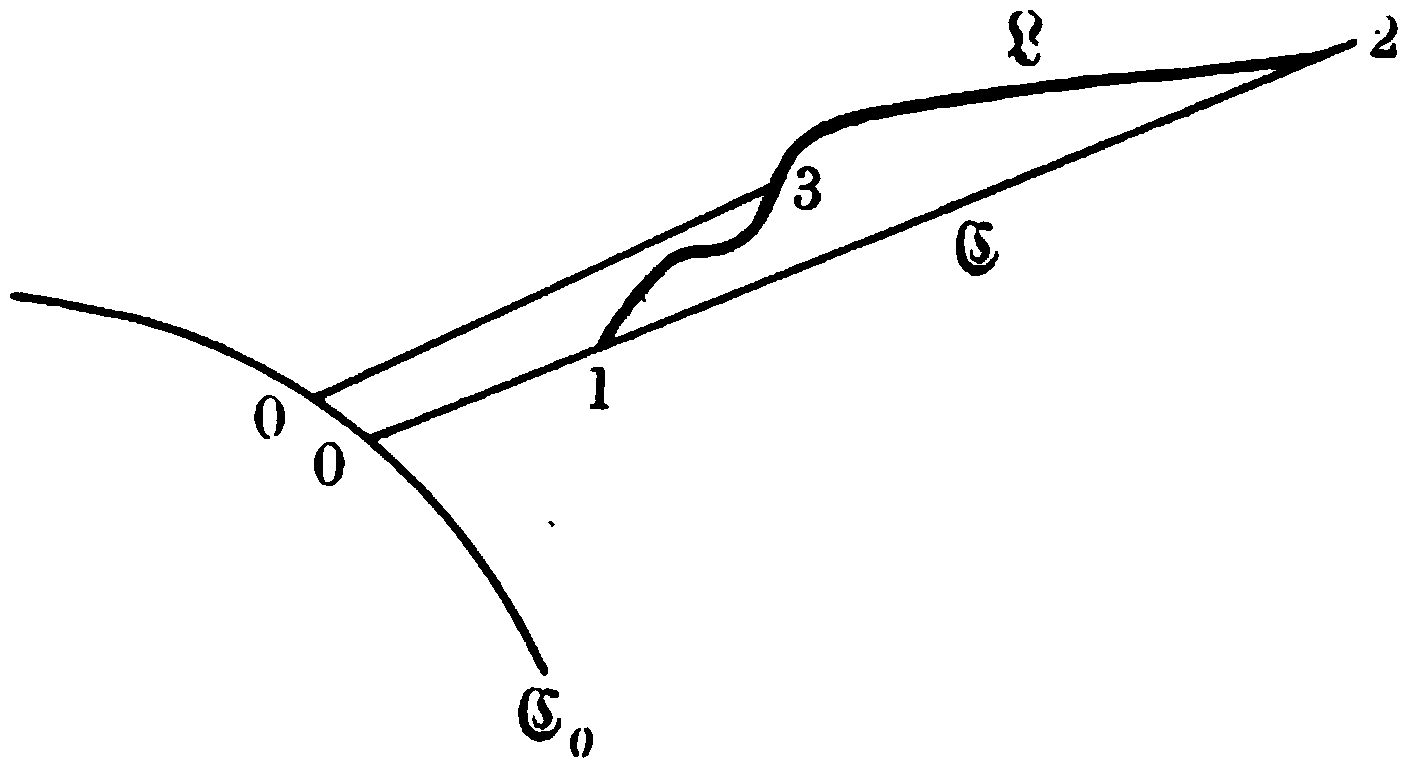
\includegraphics[width=\linewidth,height=32mm,keepaspectratio]{figures/fig08_src_clean_x8.png}
\end{minipage}\hfill
\begin{minipage}[c]{0.49\linewidth}\centering
\end{minipage}
\end{center}

用另一条属于场的曲线 $\Omega$ 连接点 1、2，点 3 沿它从 1 走向 2。该曲线具有第17节中同名曲线的性质，所以 $x_3,y_3$ 是属于该节所研究的 $\varphi(\tau)$ 类的参数 $\tau$ 的函数；参数 $t$ 沿 1 到 2 的方向增长。于是通过点 3 的每一个位置，都有场的一条确定的极值曲线；依第14节，它的参数 $a$ 以及其上对应于点 3 的论元 $t$，都是 $x_3,y_3$ 的正则函数。这条极值曲线在曲线 $\mathfrak{C}_0$ 上截出一点 0；依第14节，它的坐标以及相应论元 $t_0$ 都是 $a$ 的正则函数，并且在充分限制场和曲线段 $\mathfrak{C}_0$ 后唯一确定。因此若置
\[
\omega(a)=
F(\xi,\eta,\xi_t,\eta_t)\frac{dt_0}{da}
+F_{x'}(\xi,\ldots,\eta_t)\xi_a
+F_{y'}(\xi,\ldots,\eta_t)\eta_a\bigg|^0,
\]
则此表达式是 $a$ 的正则函数；若又置
\[
u=\overline{J}_{03},
\]
% src-pdfpage=0097
% src-break=0097
公式 (31) 给出
\[
\frac{\partial u}{\partial a}
=
\frac{\partial\overline{J}_{03}}{\partial a}
=
-\omega(a)+F_{x'}(\xi,\ldots,\eta_t)\xi_a
+F_{y'}(\xi,\ldots,\eta_t)\eta_a\bigg|^3.
\]
若设点 3 在一条确定的极值曲线 03 上移动，则立即得到
\[
\frac{\partial u}{\partial t}=F(\xi,\eta,\xi_t,\eta_t)\bigg|^3.
\]
现 $a,t$ 与 $x_3,y_3$ 一样，都是 $\tau$ 的函数，且属于第17节用 $\varphi(\tau)$ 表示的那一类；所以，若关于 $\tau$ 的每次微分总指右导数，最后两个方程给出
\[
\frac{d\overline{J}_{03}}{d\tau}
=
-\omega(a)\frac{da}{d\tau}
+F_{x'}(\xi,\ldots,\eta_t)\frac{dx}{d\tau}
+F_{y'}(\xi,\ldots,\eta_t)\frac{dy}{d\tau}\bigg|^3.
\]
又沿曲线 $\Omega$ 形成的积分 $J_{32}$，作为 $\tau$ 的函数也具有 $\varphi(\tau)$ 的性质，并满足方程
\[
\frac{dJ_{32}}{d\tau}
=
-F\left(x,y,\frac{dx}{d\tau},\frac{dy}{d\tau}\right)\bigg|^3.
\]
所以用 $x',y'$ 代替 $\xi_t,\eta_t$，得到
\[
\frac{d(\overline{J}_{03}+J_{32})}{d\tau}
=
-\omega(a)\frac{da}{d\tau}
+F_{x'}(x,y,x',y')\frac{dx}{d\tau}
\]
\[
\qquad
+F_{y'}(x,y,x',y')\frac{dy}{d\tau}
-F\left(x,y,\frac{dx}{d\tau},\frac{dy}{d\tau}\right).
\]
最后三项之和记作 $\mathfrak{E}$，更精确地写作
\[
\mathfrak{E}\left(x,y,x',y',\frac{dx}{d\tau},\frac{dy}{d\tau}\right).
\]
当点 3 分别处于其初始位置 1 和终止位置 2 时，和 $\overline{J}_{03}+J_{32}$ 的相应数值为
\[
\overline{J}_{01}+J_{12},\quad
\overline{J}_{02}=\overline{J}_{01}+\overline{J}_{12},
\]
所以两者之差为
\[
\overline{J}_{12}-J_{12}
=
\int_{\tau_1}^{\tau_2}
\frac{d(\overline{J}_{03}+J_{32})}{d\tau}\,d\tau
=
-\int_{\tau_1}^{\tau_2}\omega(a)\frac{da}{d\tau}\,d\tau
+\int_{\tau_1}^{\tau_2}\mathfrak{E}\,d\tau.
\]
但右边第一项消失；事实上，令
\[
\int \omega(a)\,da=\xi(a),
\]
% src-pdfpage=0098
% src-break=0098
则 $\xi$ 也是在 $a=a_0$ 时正则的函数，并有
\[
\int_{\tau_1}^{\tau_2}\omega(a)\frac{da}{d\tau}\,d\tau
=
\int_{\tau_1}^{\tau_2}\frac{d\xi(a)}{d\tau}\,d\tau
=
\xi(a)\bigg|_1^2.
\]
这个量的数值为 0，因为 $a$ 在点 1、2 取相同的值 $a_0$。因而
\begin{equation}\tag{54}
\overline{J}_{12}-J_{12}
=
-\int_{\tau_1}^{\tau_2}
\mathfrak{E}\left(x,y,x',y',\frac{dx}{d\tau},\frac{dy}{d\tau}\right)d\tau,
\end{equation}
而当 $\mathfrak{E}$ 具有固定符号时，左边也具有固定符号。

若在场的全部极值曲线都汇聚于点 0 的情形中，恰要检验极值曲线弧 02，则只须用固定点 0 代替曲线 $\mathfrak{C}_0$；必要时必须通过特殊考察证明的公式
\begin{equation}\tag{55}
d\overline{J}_{03}=du=F_{x'}\,dx+F_{y'}\,dy,
\end{equation}
立即给出
\begin{equation}\tag{56}
\frac{d(\overline{J}_{03}+J_{32})}{d\tau}=\mathfrak{E},\quad
J_{02}-\overline{J}_{02}
=
-\int_{\tau_0}^{\tau_2}\mathfrak{E}\,d\tau,
\end{equation}
只要用来比较的曲线 $\Omega$ 留在从点 0 出发的极值曲线所简单覆盖的面积区域内。

依第15节，即使曲线 $\mathfrak{C}_0$ 被场的极值曲线横截（图9），$du$ 的简单公式 (55) 仍然成立；此时 $\omega(a)$ 恒等消失。

\begin{center}
{\small 图~9}\par\vspace{1mm}
\begin{minipage}[c]{0.47\linewidth}\centering
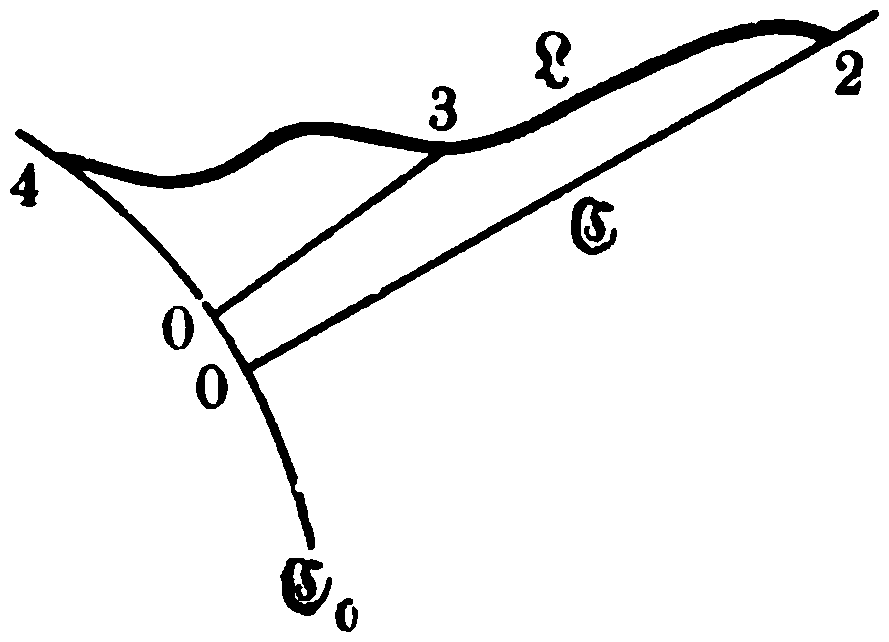
\includegraphics[width=\linewidth,height=32mm,keepaspectratio]{figures/fig09_src_clean_x8.png}
\end{minipage}\hfill
\begin{minipage}[c]{0.49\linewidth}\centering
\end{minipage}
\end{center}

我们利用这一点，通过表达式 $\mathfrak{E}$ 也导出具有可变边界的极值判据。设点 4 位于曲线 $\mathfrak{C}_0$ 上，点 2 如前位于曲线 $\mathfrak{C}$ 上；两点由一条留在场内的曲线 $\Omega$ 相连，点 3 沿它从 4 到 2 的方向移动。那么和 $\overline{J}_{03}+J_{32}$ 的初值与终值分别为
\[
J_{42},\quad \overline{J}_{02},
\]
% src-pdfpage=0099
% src-break=0099
并且如前有
\[
\frac{d\overline{J}_{03}}{d\tau}
=
F_{x'}\frac{dx}{d\tau}
+F_{y'}\frac{dy}{d\tau},
\quad
\frac{dJ_{32}}{d\tau}
=
-F\left(x,y,\frac{dx}{d\tau},\frac{dy}{d\tau}\right),
\]
所以
\begin{equation}\tag{57}
J_{42}-\overline{J}_{02}
=
-\int_{\tau_4}^{\tau_2}\mathfrak{E}\,d\tau.
\end{equation}

\begin{center}{\large \S~21.}\end{center}

由以上可见，考察量 $\mathfrak{E}$ 就能决定极值是否发生；它显然依赖于点 2 $(x,y)$ 以及从该点出发的两个线元，这两个线元分别由场的极值曲线和曲线 $\Omega$ 上参数 $t$、$\tau$ 增大的方向来规定。若 $x'$ 和 $\dfrac{dx}{d\tau}$ 都不为零，从而可以置
\[
D x=\frac{dx}{d\tau}\,d\tau,\quad
D y=\frac{dy}{d\tau}\,d\tau=\bar{p}\,D x,\quad
dy=p\,dx,
\]
\[
F(x,y,x',y')dt=f(x,y,p)dx,
\]
\[
F\left(x,y,\frac{dx}{d\tau},\frac{dy}{d\tau}\right)d\tau
=
f(x,y,\bar{p})D x,
\]
则得到
\begin{equation}\tag{58}
\mathfrak{E}\,d\tau
=
\{f(x,y,p)+(\bar{p}-p)f_p(x,y,p)-f(x,y,\bar{p})\}D x.
\end{equation}
诚然，表征第一个线元的量 $x'$、$y'$ 只出现在 $F_{x'}$、$F_{y'}$ 中，而这些表达式只依赖于 $x':y'$。但不能由此断定：若用极值曲线弧元的反向弧元代替它，$\mathfrak{E}$ 的数值仍不变；因为即使 $F$ 是 $x'$、$y'$ 的单值函数，$F_{x'}$、$F_{y'}$ 也未必是 $x':y'$ 的单值函数（第3节）。所以诸量
\[
\mathfrak{E}\left(x,y,x',y',\frac{dx}{d\tau},\frac{dy}{d\tau}\right),\quad
\mathfrak{E}\left(x,y,-x',-y',\frac{dx}{d\tau},\frac{dy}{d\tau}\right)
\]
不必相等，正如诸量
\[
\mathfrak{E}\left(x,y,x',y',\frac{dx}{d\tau},\frac{dy}{d\tau}\right),\quad
\mathfrak{E}\left(x,y,x',y',-\frac{dx}{d\tau},-\frac{dy}{d\tau}\right)
\]
也不必互为相反数（见下文各例）。

% src-pdfpage=0100
% src-break=0100
$\mathfrak{E}$ 所依赖的两个线元恰在存在一个正量 $\alpha$ 满足方程
\begin{equation}\tag{59}
x'=\alpha\frac{dx}{d\tau},\quad
y'=\alpha\frac{dy}{d\tau}
\end{equation}
时，并且只有此时，才彼此重合。在这种情形下，有
\[
F_{x'}(x,y,x',y')
=
F_{x'}\left(x,y,\frac{dx}{d\tau},\frac{dy}{d\tau}\right),
\]
\[
F_{y'}(x,y,x',y')
=
F_{y'}\left(x,y,\frac{dx}{d\tau},\frac{dy}{d\tau}\right).
\]
又因为总有
\[
\frac{dx}{d\tau}F_{x'}\left(x,y,\frac{dx}{d\tau},\frac{dy}{d\tau}\right)
\]
\[
+
\frac{dy}{d\tau}F_{y'}\left(x,y,\frac{dx}{d\tau},\frac{dy}{d\tau}\right)
-
F\left(x,y,\frac{dx}{d\tau},\frac{dy}{d\tau}\right)=0,
\]
所以
\[
\mathfrak{E}=0.
\]
这时称 $\mathfrak{E}$ 以通常方式消失。若 $\mathfrak{E}$ 取值为零，但方程 (59) 对任何正的 $\alpha$ 值都不成立，则称它异常消失。

若预先采用一个以后将在第30节证明、而此处不再使用的事实，即一段充分小的极值曲线一般都可被一个场包围，则可以从几何上说明量 $\mathfrak{E}$ 的意义。设 78、79 是分别属于值组 $(x,y,dx,dy)$、$(x,y,Dx,Dy)$ 的线元（图10）；

\begin{center}
{\small 图~10}\par\vspace{1mm}
\begin{minipage}[c]{0.47\linewidth}\centering
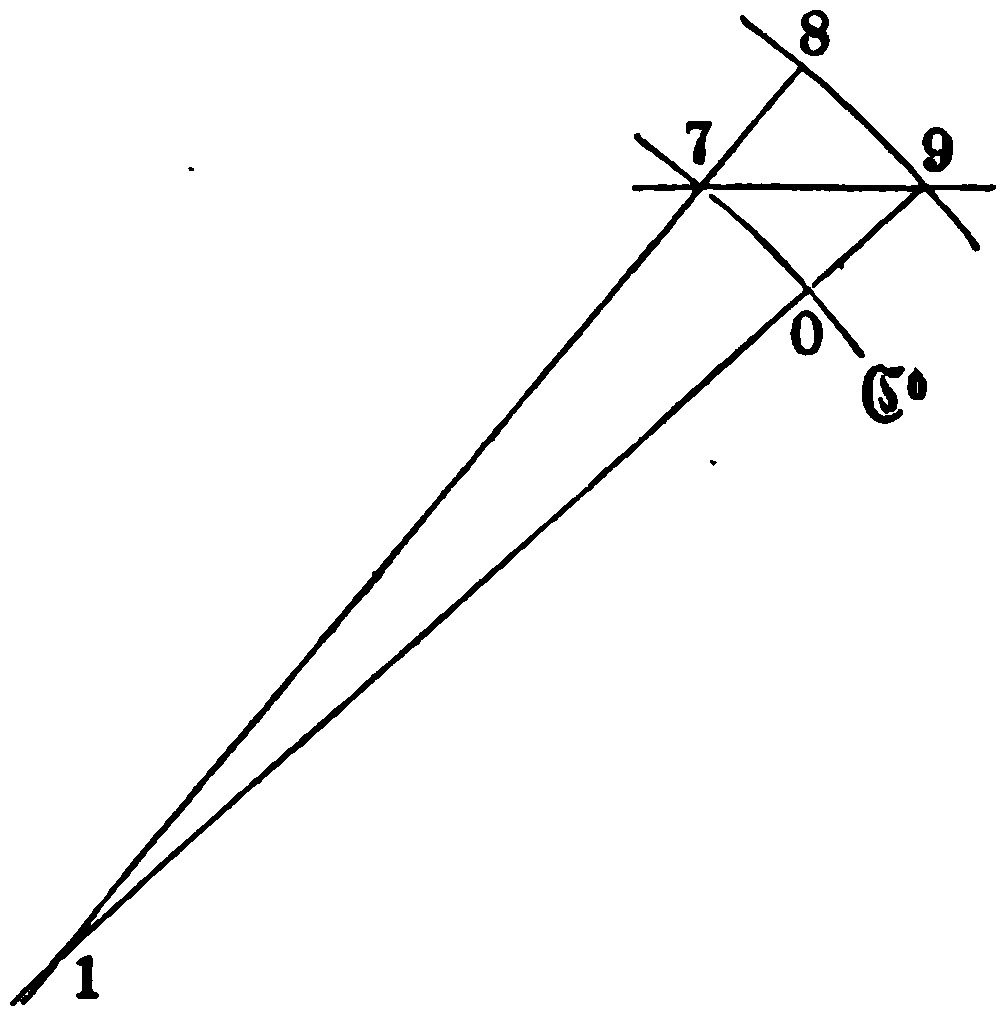
\includegraphics[width=\linewidth,height=32mm,keepaspectratio]{figures/fig10_src_clean_x8.png}
\end{minipage}\hfill
\begin{minipage}[c]{0.49\linewidth}\centering
\end{minipage}
\end{center}

于是沿方向 78 作一条极值曲线，并在点 7 的邻域内用一个场包围它；令场的极值曲线横截通过点 7 的曲线 $\mathfrak{C}^0$ 以及一条曲线 89。前一曲线在点 0 被场中通过 9 的极值曲线相交；于是 $\overline{J}_{09}$ 或 $\overline{J}_{78}$ 可以看作从曲线 $\mathfrak{C}^0$ 起算的量 $u$ 的微分，按照

% exit seam: source-PDF101 continues the same sentence; no PDF101 body is owned here.
% END PHYSICALLY EMBEDDED BODY INH02 1/1
\endgroup
\KneserUnitEnd{INH02}
\clearpage
\KneserUnitStart{INH03}
\begingroup
\KneserInheritedLayout\KneserTagsLeft\KneserReportTagSide{INH03}
\setcounter{equation}{0}
% Historical Fraktur macros preserved from the accepted source wrapper.
\KneserHistoricalFraktur
\typeout{KNESER-MACRO-MODE:INH03:FRAKTUR-COS-SIN-TG-CTG-tg}
% BEGIN PHYSICALLY EMBEDDED BODY INH03 1/5: inherited/INH03_pdf101_150_producer_r3_fraktur/work/zh_101_125.tex
% src-pdfpage=0101
% src-break=0101
\S~15 的意义来理解，并由公式 (34) 得
\[
\overline{J}_{09}=\overline{J}_{78}
=
F_{x'}(x,y,dx,dy)D x+F_{y'}(x,y,dx,dy)D y.
\]
若极值曲线 78 与 09 相交于点 1，且从点 7 看去，点 1 与点 8 位于相反的一侧，则由 \S~15 有
\[
\overline{J}_{17}=\overline{J}_{10},\quad
\mathfrak{E}\,d\tau
=
\overline{J}_{78}-J_{79}
=
\overline{J}_{19}-\overline{J}_{17}-J_{79}.
\]
由此可见，量 $\mathfrak{E}d\tau$ 与坐标系无关；这一点也可由 \S~16 中导出的恒等式
\[
F_{x'}(x,y,dx,dy)D x+F_{y'}(x,y,dx,dy)D y
\]
\[
=
G_{u'}(u,v,du,dv)D u+G_{v'}(u,v,du,dv)D v
\]
看出。

特别地，可以设想将坐标系旋转到如下位置：对于两个弧元 78 与 79，微分 $dx$ 具有相同符号；也就是说，两个弧元都指向一条平行于 $y$ 轴的直线的同一侧。于是
\[
p=\frac{dy}{dx},\quad
\bar{p}=\frac{dy}{d\tau}:\frac{dx}{d\tau}=D y:D x
\]
都是有限量，而这两个弧元分别由数值组 $(x,y,p,dx)$、$(x,y,\bar{p},dx)$ 确定。若 $F$ 对所有从点 $(x,y)$ 出发的弧元都是正则的，则依 \S~5，
\[
f(x,y,p)=\frac{F}{x'}
\]
对于落在方向 78 与 79 所成凹角内的一切弧元也都是正则的，因为对这些弧元 $x'$ 不为零。因此，$f$ 在从 $p$ 到 $\bar{p}$ 的区间上正则；若 $\theta$ 为真分数，便可依 (58) 写成
\[
f(x,y,\bar{p})=f(x,y,p)+(\bar{p}-p)f_p(x,y,p)
+\frac{1}{2}(\bar{p}-p)^2 f_{pp}[x,y,p+\theta(\bar{p}-p)],
\]
\begin{equation}\tag{60}
\mathfrak{E}d\tau
=
-\frac{1}{2}(\bar{p}-p)^2 f_{pp}[x,y,p+\theta(\bar{p}-p)]\,dx.
\end{equation}
当强极值的勒让德条件成立时，量 $\mathfrak{E}$ 具有 $-F_1$ 的固定符号，并且只以通常方式消失；这是因为乘积
\[
f_{pp}[x,y,p+\theta(\bar{p}-p)]\,dx
\]
恒等于量 $F_1(x,y,dx,dy)dx^4$，后者属于经过点 $(x,y)$ 且分量为
\[
dx,\ [p+\theta(\bar{p}-p)]dx=dy
\]
% src-pdfpage=0102
% src-break=0102
的弧元。这就证明了上述断言。然而，如果只假定弱极值的勒让德条件成立，那么 $\mathfrak{E}$ 仅在如下范围内具有上述两项性质：决定其值的两个弧元 78、79，在位置和方向上都与曲线 $\mathfrak{C}$ 上按积分方向取定的某个弧元充分接近。反过来，却不能以同样方式由量 $\mathfrak{E}$ 的符号推出量 $F_1$ 的符号。



\begin{center}{\large \S~22.}\end{center}

一般而言，若 $t$ 与 $a$ 对应于沿曲线 $\Omega$ 运动的点 3，则有
\[
x=\xi(t,a),\quad y=\eta(t,a),
\]
\[
\frac{dx}{d\tau}=\xi_t\frac{dt}{d\tau}+\xi_a\frac{da}{d\tau},\quad
\frac{dy}{d\tau}=\eta_t\frac{dt}{d\tau}+\eta_a\frac{da}{d\tau},
\]
\[
x'=\xi_t,\quad y'=\eta_t.
\]
若沿整条曲线 $\Omega$ 的量 $\mathfrak{E}$ 在每一点都以通常方式消失，就会得到方程 (59)，从而有
\[
\begin{vmatrix}
x' & \dfrac{dx}{d\tau}\\[0.7em]
y' & \dfrac{dy}{d\tau}
\end{vmatrix}
=
\begin{vmatrix}
\xi_t & \xi_a\dfrac{da}{d\tau}\\[0.7em]
\eta_t & \eta_a\dfrac{da}{d\tau}
\end{vmatrix}
=
\Delta\frac{da}{d\tau}=0.
\]
由于 $\Delta$ 不为零，故在参数 $\tau$ 的一个有限区间内
\[
\frac{da}{d\tau}=0.
\]
又因 $a$ 作为 $\tau$ 的函数，具有 \S~17 中定义的函数 $\varphi(\tau)$ 的性质，所以 $a$ 必须沿整条曲线 $\Omega$ 保持常数，并等于其初值 $a_0$。

因此，若曲线 $\Omega$ 不与 $\mathfrak{C}$ 完全重合；量 $\mathfrak{E}$ 的异常消失或者本来就不可能，或者已由对曲线 $\Omega$ 的限制排除；并且沿 $\Omega$ 以通常方式消失时不发生符号改变，那么 \S~20 中方程 (54)、(56)、(57) 的右端均不为零，并且
% src-pdfpage=0103
% src-break=0103
具有固定符号。因而，相对于按上述方式加以限制的曲线 $\Omega$，极值曲线 12、02 确实使积分 $J$ 取得极值；当 $\mathfrak{E}$ 为正时是最大值，为负时是最小值。

特别地，若曲线 $\Omega$ 位于依 \S~17 由 $\rho$ 与 $\rho_1$ 定义的、弧段 12 的一个更小邻域内，则曲线 $\mathfrak{C}$ 上按 $t$ 增大方向取向的切线，与场中某条极值曲线上同向切线相比，只要二者切点的距离小于 $\rho$，夹角就小于某个界 $\rho_2$；这个界随 $\rho$ 无界地趋于零。曲线 $\Omega$ 的每条切线又对应于弧段 12 的一条切线，二者切点的距离也小于 $\rho$，夹角不超过 $\rho_1$。所以，曲线 $\Omega$ 的切线与通过其切点的场中极值曲线的夹角小于 $\rho_1+\rho_2$，只要把邻域限制得充分小，这个夹角就可以任意小。为了保证弱极值，只须量 $\mathfrak{E}$ 在决定其值的两个线元彼此任意接近、且与曲线 $\mathfrak{C}$ 上按积分方向取定的一个弧元任意接近时具有固定符号，并且只以通常方式消失。在 \S~17 的情形 a) 中，这项规定可以取代关于 $F_1$ 的条件；后者依 \S~21 可推出前者。

此外，要由 \S~20 的方程 (54)、(56)、(57) 推出强极值，首先必须要求被积函数对场中任意方向的线元都是正则的；其次，量 $\mathfrak{E}(x,y,x',y',D x,D y)$ 必须具有上述性质，其中 $(D x,D y)$ 是从点 $(x,y)$ 出发的任意线元，而 $x',y'$ 属于场中经过该点的极值曲线。因此，在先前于 \S~17 建立的强极值判据中，情形 b) 的勒让德条件可以由要求较弱的魏尔斯特拉斯条件取代：量 $\mathfrak{E}(x,y,x',y',D x,D y)$ 在包含弧段 02 的某个区域内的每一点都具有固定符号，并且只在线元 $(x',y')$ 与 $(D x,D y)$ 重合时消失。

在情形 a) 和 b) 中，还可以取消 \S~16 与 17
% src-pdfpage=0104
% src-break=0104
中曾实质使用的“被积函数 $F$ 不消失”这一要求，因为当前的推导显然与此假设无关。

\begin{center}{\large \S~23.}\end{center}

\noindent\textbf{例题。问题 I（\S~9）。} 这里取正平方根，并置
\[
F=\sqrt{x'^2+y'^2},
\]
\[
\mathfrak{E}
=
\frac{x'}{\sqrt{x'^2+y'^2}}\frac{dx}{d\tau}
+
\frac{y'}{\sqrt{x'^2+y'^2}}\frac{dy}{d\tau}
-
\sqrt{\left(\frac{dx}{d\tau}\right)^2+\left(\frac{dy}{d\tau}\right)^2}
\]
\[
=
\sqrt{\left(\frac{dx}{d\tau}\right)^2+\left(\frac{dy}{d\tau}\right)^2}
\{\cos(ds,Ds)-1\},
\]
其中 $ds,Ds$ 是分别对应于正微分 $dt,d\tau$ 的弧元。因此，量 $\mathfrak{E}$ 从不为正，并且只在 $ds$ 与 $Ds$ 重合时消失。若在 \S~21 的公式 (58) 中置
\[
Fdt=\sqrt{1+p^2}\,dx,\quad
F\left(x,y,\frac{dx}{d\tau},\frac{dy}{d\tau}\right)d\tau
=
\sqrt{1+\bar{p}^2}\,D x,
\]
也会得到同一结论；此处各平方根必须取其旁边微分的符号。于是
\[
\mathfrak{E}d\tau
=
\left\{\sqrt{1+p^2}+\frac{(\bar{p}-p)p}{\sqrt{1+p^2}}-\sqrt{1+\bar{p}^2}\right\}D x
\]
\[
=
\sqrt{1+\bar{p}^2}\,D x
\left\{\frac{\bar{p}p+1}{\sqrt{1+p^2}\sqrt{1+\bar{p}^2}}-1\right\},
\]
这个表达式也从不为正，因为
\[
\sqrt{1+\bar{p}^2}\,D x
\]
为正，而它旁边的括号因不等式
\[
(1+p\bar{p})^2\leq (1+p^2)(1+\bar{p}^2).
\]
而为负或为零。依 \S~21，这一结果在几何上意味着：在三角形 179 中，当边 79 相对于另两边很小时，有不等式
\begin{equation}\tag{61}
\overline{J}_{19}-\overline{J}_{17}-J_{79}<0
\end{equation}
成立；即边 17 与 79 之和大于边 19。在本题中，用表达式 $\mathfrak{E}$ 证明
% src-pdfpage=0105
% src-break=0105
极值成立的论证，可以作完全初等的几何解释。设 145 为一直线上的三个点（图~11），7、9 是点 2 的两个位置，而点 2 沿任意曲线 45 从 4 向 5 运动，

% unit: fig11 source=kneser_lvr_1900_archiveorg.pdf#p0105 authorial=true type=hq_sourcecrop


\begin{center}
{\small 图~11.}\par\vspace{1mm}
\begin{minipage}[c]{0.47\linewidth}\centering
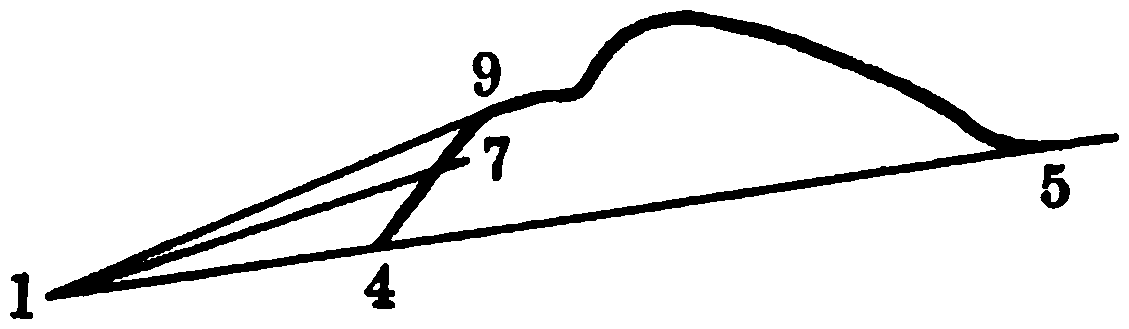
\includegraphics[width=\linewidth,height=32mm,keepaspectratio]{figures/fig11_accepted_derivative.png}
\end{minipage}\hfill
\begin{minipage}[c]{0.49\linewidth}\centering
\end{minipage}
\end{center}

若以 $\overline{J}$ 表示直线段的长度，则由 (61) 有
\[
\overline{J}_{17}+J_{75}>\overline{J}_{19}+J_{95},
\]
所以量 $J_{13}+J_{23}$ 减小，并且在点 2 开始运动时的值大于运动结束时的值。



\noindent\textbf{问题 II（\S~9）。} 量 $\mathfrak{E}$ 与问题 I 中所得的量只相差一个正因子 $y$，所以强最小值的魏尔斯特拉斯条件成立。

引入双曲函数，并置
\[
\Cof z=\frac{e^z+e^{-z}}{2},\quad
\Sin z=\frac{e^z-e^{-z}}{2},\quad
\Tg z=\frac{1}{\Ctg z}=\frac{\Sin z}{\Cof z},
\]
其中有等式
\[
\Cof^2z-\Sin^2z=1,\quad
d\Cof z=\Sin z\,dz,\quad
d\Sin z=\Cof z\,dz,
\]
\[
d\Tg z=\frac{dz}{\Cof^2z},\quad
d\Ctg z=\frac{-dz}{\Sin^2z}
\]
成立。极值曲线满足方程
\begin{equation}\tag{62}
y=a\Cof\frac{x-b}{a},\quad
p=\Sin\frac{x-b}{a}.
\end{equation}
我们特别考察那些横截给定曲线 $\mathfrak{C}_0$，即与之正交相交（\S~11）的极值曲线。设该曲线的方程为
\[
y_0=f(x_0);
\]
则正交相交的极值曲线的常数满足
\[
y_0=a\Cof\frac{x_0-b}{a},\quad
1+p_0f'(x_0)=0
\]
；或者，若置
\[
u=\frac{x-b}{a},\quad u_0=\frac{x_0-b}{a}
\]
，则
% src-pdfpage=0106
% src-break=0106
\begin{equation}\tag{63}
f(x_0)=a\Cof u_0,\quad
1+f'(x_0)\Sin u_0=0.
\end{equation}
在这里以及 (62) 的第一个方程中，对 $x,x_0,a,b$ 微分，得到
\[
dy=\Sin u\,dx+0\,dx_0+(\Cof u-u\Sin u)\,da-\Sin u\,db,
\]
\[
0=[\Sin u_0-f'(x_0)]\,dx_0+(\Cof u_0-u_0\Sin u_0)\,da-\Sin u_0\,db,
\]
\begin{equation}\tag{64}
0=
\left[\frac{f'(x_0)}{a}\Cof u_0+f''(x_0)\Sin u_0\right]dx_0
-\frac{f'(x_0)}{a}u_0\Cof u_0\,da
-\frac{f'(x_0)}{a}\Cof u_0\,db.
\end{equation}
最后两个方程中含 $da,db$ 的各项之行列式为
\[
M=
\frac{f'(x_0)\Cof u_0}{a}
\begin{vmatrix}
\Cof u_0-u_0\Sin u_0 & -\Sin u_0\\
-u_0 & -1
\end{vmatrix}
=
\frac{f'(x_0)\Cof^2u_0}{-a},
\]
所以，只要曲线 $\mathfrak{C}_0$ 在所考察的位置不平行于 $x$ 轴——我们将作此假设——该行列式便不为零。因此，可以设想由方程 (63) 把 $a$ 与 $b$ 确定为 $x_0$ 的正则函数，并将 $y$ 表成 $x$ 与 $x_0$ 的函数。此外，由于沿每条悬链线，$y$ 都是 $x$ 的单值函数，可以置 $t=x$；于是，对与 $\mathfrak{C}_0$ 正交相交的极值曲线族，有
\[
\Delta=\frac{\partial(x,y)}{\partial(x,x_0)}=\frac{\partial y}{\partial x_0},\quad
dy=p\,dx+\Delta\,dx_0.
\]
由方程 (64)，通过初等运算消去 $da$ 与 $db$，得到
\[
M\,dy=M\Sin u\,dx+dx_0(\ldots),
\]
其中 $dx_0$ 的系数，是上述方程中 $dx_0,da,db$ 的系数行列式；因而
\[
M\Delta=
\begin{vmatrix}
0 & \Cof u-u\Sin u & -\Sin u\\
\Sin u_0-f'(x_0) & \Cof u_0-u_0\Sin u_0 & -\Sin u_0\\
\dfrac{f'(x_0)}{a}\Cof u_0+f''(x_0)\Sin u_0 &
-\dfrac{f'(x_0)}{a}u_0\Cof u_0 &
-\dfrac{f'(x_0)}{a}\Cof u_0
\end{vmatrix}.
\]
只要这个表达式不消失，在点 0 与曲线 $\mathfrak{C}_0$ 正交相交的极值弧 02，就相对于一切连接 $\mathfrak{C}_0$ 与点 2 的曲线，使回转曲面取得强最小值。

再考虑 (63) 的第二个方程，并置
% src-pdfpage=0107
% src-break=0107
\[
\frac{f''(x_0)}{\left(\sqrt{1+[f'(x_0)]^2}\right)^3}
=
\frac{f''(x_0)}{(1+\Sin^{-2}u_0)^{3/2}}
=
f''(x_0)\Tg^3u_0
=
\frac{1}{r},
\]
则 $|r|$ 是曲线 $\mathfrak{C}_0$ 的曲率半径，并可写成
\[
M\Delta
=
-\frac{\Cof^3u_0}{r\Sin^2u_0}
\begin{vmatrix}
\Cof u-u\Sin u & \Sin u\\
\Cof u_0-u_0\Sin u_0 & \Sin u_0
\end{vmatrix}
\]
\[
\qquad
+\frac{\Cof^2u_0}{y_0\Sin u_0}
\begin{vmatrix}
0 & \Cof u-u\Sin u & -\Sin u\\
\Cof u_0\Ctg u_0 & \Cof u_0-u_0\Sin u_0 & -\Sin u_0\\
-1 & u_0 & 1
\end{vmatrix}.
\]
当 $\mathfrak{C}_0$ 缩为一个无穷小圆时，$r=0$，而方程 $\Delta=0$ 要求
\[
\begin{vmatrix}
\Cof u-u\Sin u & \Sin u\\
\Cof u_0-u_0\Sin u_0 & \Sin u_0
\end{vmatrix}
=0,\quad
\Ctg u-u=\Ctg u_0-u_0
\]
，或者
\[
\frac{y}{p}-x=\frac{y_0}{p_0}-x_0;
\]
这个方程表示，极值曲线在点 0 与 $(x,y)$ 处的切线相交于 $x$ 轴上。因此，只要弧段 02 的任意两条切线都不出现这种情形，通过点 0 的极值曲线就构成每个弧段 12 的场，其中弧段 12 是 02 的一部分。由于点 0 与 1 可以任意接近，故极值曲线上任一弧段，只要其任意两条切线不在 $x$ 轴上相交，就在端点固定时给出一个极值。

在曲线 $\mathfrak{C}_0$ 具有有限曲率的一般情形下，方程 $\Delta=0$ 具有形式
\[
A(\Cof u-u\Sin u)+B\Sin u=0,
\]
其中 $A$ 与 $B$ 只依赖于 $u_0,y_0$ 及 $1:r$，并且关于最后一个量是线性的。若 $A$ 不为零，则方程可写成
\begin{equation}\tag{65}
\Ctg u-u+\frac{B}{A}=0;
\end{equation}
其左端的导数为
\[
-\frac{1}{\Sin^2u}-1,
\]
所以它随 $u$ 的增大而不断减小。又容易求得
% src-pdfpage=0108
% src-break=0108
\[
\Ctg(\mp\infty)=\mp1,\quad \Ctg(\pm0)=\pm\infty,
\]
因此，当
\[
|B|>|A|,
\]
时，方程 (65) 有唯一的有限根；否则没有根。再把 $u_0$ 与 $y_0$ 固定，也就是固定点 0 以及曲线 $\mathfrak{C}_0$ 的方向，则可以选取该曲线的曲率，使 $B:A$ 取得任意给定值。因此，总可以适当地选择 $r$，使与曲线 $\mathfrak{C}_0$ 正交的极值曲线到给定点 2 为止时，不再能保证相对于一切连接 $\mathfrak{C}_0$ 与点 2 的曲线给出最小值。

\noindent\textbf{问题 IV（\S~9）。} 设 $\Omega$ 是 $wy$ 平面内的一条任意曲线：它从点 $w=y=0$ 出发，穿过半平面 $y>0$，再下降到直线 $y$，并具有 \S~17 中同名曲线所具的连续性。若参数 $\tau$ 在坐标原点取值 $\tau_0$，并用 $w$ 代替 \S~9 中的符号 $u$，则取正平方根时
\begin{equation}\tag{66}
x=\int_{\tau_0}^{\tau}
y\sqrt{\left(\frac{dw}{d\tau}\right)^2+\left(\frac{dy}{d\tau}\right)^2}\,d\tau
\end{equation}
，因而必有
\begin{equation}\tag{67}
x\geq \int_{\tau_0}^{\tau}y\frac{dy}{d\tau}\,d\tau,\quad
x\geq \frac{y^2}{2}.
\end{equation}
等号仅当在 $\tau_0$ 与 $\tau$ 之间恒有
\[
\frac{dw}{d\tau}=0
\]
时成立。于是，相应的曲线 $\Omega_1$ 在 $xy$ 平面内位于第一象限 $(x>0,y>0)$，并处在抛物线
\begin{equation}\tag{68}
y^2=2x.
\end{equation}
的内部，即其凹侧。从点 $0(x=y=0)$ 出发的极值曲线
\begin{equation}\tag{69}
1-\frac{x}{a^2}
=
\sqrt{1-\left(\frac{y}{a}\right)^2},\quad
\frac{x^2}{a^2}=2x-y^2
\end{equation}
恰好将该抛物线的内部单重覆盖，因为这些方程给出唯一的正 $a^2$ 值，只要给定 $x,y$ 且
% src-pdfpage=0109
% src-break=0109
$2x-y^2$ 为正。若曲线 $\Omega$ 起初有一段平行于 $y$ 轴，则曲线 $\Omega_1$ 有一段相应的弧 01 与抛物线 (68) 重合，这一段对 $J$ 的贡献为零。因此，若 3 是曲线 $\Omega_1$ 的终点，即 $y_3=0$，则沿该曲线有
\begin{equation}\tag{70}
J_{03}=J_{13}.
\end{equation}
曲线 $\Omega_1$ 一旦离开抛物线，就不能再次到达它，因为此后 $dw:d\tau$ 至少在某一段上不为零，关系式 (67) 中的等号便不再成立。

椭圆 (69) 在抛物线 (68) 的 $y>0$ 那一半内部构成一个场；因为这里
\[
x=\xi=t,\quad
y=\eta=\sqrt{2t-\left(\frac{t}{a}\right)^2},
\]
从而
\[
\Delta=\frac{\partial(\xi,\eta)}{\partial(t,a)}
=\frac{\partial y}{\partial a}
=
\frac{t^2}{a^3}\left(2t-\frac{t^2}{a^2}\right)^{-1/2},
\]
这个值显然不为零。此外，若 $a$ 与平方根均取正，而 2 是所考察区域中的任一点，则
\begin{equation}\tag{71}
u=\overline{J}_{02}
=
\int_0^x y\sqrt{1-y^2p^2}\,dx
=
\int_0^x\frac{y^2}{a}\,dx
=
\frac{x^2}{a}-\frac{x^3}{3a^3}
\end{equation}
。利用方程 (69) 把 $dy$ 表成 $dx$ 与 $da$，并令 $x',y',p$ 属于场中的极值曲线，即可容易验证
\[
F_{x'}=a,\quad F_{y'}=-ay^2p,\quad du=F_{x'}dx+F_{y'}dy;
\]
由此，当点 2 沿曲线 $\Omega_1$ 从 1 运动到 3 时，
\[
d(\overline{J}_{02}+J_{23})=\mathfrak{E}\,d\tau,
\]
而依公式 (58)，若 $D x$ 与 $\bar{p}$ 属于曲线 $\Omega_1$，$p$ 属于极值曲线，则
\[
\mathfrak{E}d\tau
=
y\left\{
\frac{1-y^2p\bar{p}}{\sqrt{1-y^2p^2}}
-
\sqrt{1-y^2\bar{p}^2}
\right\}D x,
\]
其中分母中的平方根为正。对每个需要考虑的方向，量
% src-pdfpage=0110
% src-break=0110
\[
y\frac{dy}{dx}
=
\frac{dy}{\sqrt{dy^2+dw^2}}
\]
位于界限 $\pm1$ 之间；在场中极值曲线上，只有当 $y=0$ 时才达到这些界限。因此，只要 $y$ 不消失，$y^2p\bar{p}$ 就是真分数，量 $1-y^2p\bar{p}$ 为正。由于 $y$ 与 $D x$ 为正，$\mathfrak{E}d\tau$ 显然也为正，只要 $\sqrt{1-y^2\bar{p}^2}$ 为负；若该平方根为正，则由一般不等式
\[
(1-\alpha\beta)^2\geq(1-\alpha^2)(1-\beta^2),
\]
可知 $\mathfrak{E}d\tau$ 从不为负，并且只在 $p=\bar{p}$ 时消失，即只以通常方式消失，因为属于极值曲线的微分 $dx$ 与 $D x$ 同为正。若等式
\[
1-y^2\bar{p}^{\,2}=0,
\]
成立，则用 $x,y$ 表示的积分 $J$ 的被积函数虽是奇异的，但原始定义
\[
J=\int y^2\frac{dw}{d\tau}\,d\tau
=
\int y\sqrt{1-y^2\bar{p}^{\,2}}\frac{dx}{d\tau}\,d\tau
\]
表明，$J_{23}$ 仍是 \S~17 意义下的函数 $\varphi(\tau)$。此时量 $dJ_{23}$ 消失；而 $du$ 具有表达式
\[
du=a(1-y^2p\bar{p})\,dx,
\]
所以仍为正。因此，若 $\mathfrak{E}$ 在曲线 $\Omega_1$ 上并非处处以通常方式消失，即该曲线不与某条极值曲线 (69) 重合，则当点 2 位于 1 与 3 之间时，量 $\overline{J}_{02}+J_{23}$ 不断增大；当然，在点 1 与 3 本身，上述考察不再适用。当点 2 趋近位置 1 或 3 时，该量分别趋于极限值 $J_{13}$ 与 $\overline{J}_{03}$；因为当点 2 趋近抛物线上的某个确定位置时，由公式 (69)、(71) 有
\[
\lim\frac{x}{a}=0,\quad \lim u=\lim\overline{J}_{02}=0.
\]
结合关系式 (70)，由量 $\mathfrak{E}$ 的性态可得：若 $\Omega_1$ 不是曲线 (69) 中的一条，则
% src-pdfpage=0111
% src-break=0111
\[
\overline{J}_{03}>J_{13},\quad
\overline{J}_{03}>J_{013},
\]
即球的体积大于由曲线 $\Omega$ 旋转所得、且具有相同表面积的立体的体积。

% src-pdfpage=0111 portion=lower
% unit: sec24 source=kneser_lvr_1900_archiveorg.pdf#p0111 authorial=true
\begin{center}{\large \S~24.}\end{center}

沿曲线 $\mathfrak{C}$ 从点 0 按 $t$ 增大的方向前进，设 6 是离开 0 后量 $\Delta$ 首次消失的点。我们假定，这件事发生在函数 $\xi$ 与 $\eta$ 沿曲线 $\mathfrak{C}$ 丧失其既定性质之前；于是 6 仍是该曲线的正则点。在它的邻域内，可用不等式
\[
|t-t_6|<\varepsilon,\quad |a-a_0|<\varepsilon
\]
为量 $t,a$ 定义一个区域；在此区域中，函数 $\xi,\eta,F(\xi,\eta,\xi_t,\eta_t)$ 保持正则，且量 $\xi_t^2+\eta_t^2$ 不为零。相应的点 $(x,y)$ 由方程
\[
x=\xi(t,a),\quad y=\eta(t,a)
\]
确定；这些点不再属于曲线 $\mathfrak{C}$ 某一部分的场，因为一般说来，它们会将平面的某些区域双重覆盖。仍设曲线 $\mathfrak{C}_0$ 从点 0 开始，并被场中极值曲线横截；我们称 6 为曲线 $\mathfrak{C}_0$ 在极值曲线 $\mathfrak{C}$ 上的极值焦点。若曲线 $\mathfrak{C}_0$ 缩为点 0，从而场中所有极值曲线都通过该点，则称 0 与 6 为共轭点，更完整地说是极值共轭点。例如，依 \S~23，在问题 II 中，共轭点的特征是它们的切线相交于 $x$ 轴；任意曲线 $\mathfrak{C}_0$ 的极值焦点则由容易讨论的方程 (65) 确定。

共轭点与焦点的重要性质基于以下事实：量 $\Delta$ 满足一个仅由极值曲线 $\mathfrak{C}$ 决定的线性微分方程。量 $\Delta$ 的几何意义把我们引向这个方程；这一意义可由下列考察看出。设
% src-pdfpage=0112
% src-break=0112
\begin{equation}\tag{72}
\begin{aligned}
x&=\xi(t,a),\quad y=\eta(t,a),\\
\bar x&=\xi(t,a+\delta a),\quad \bar y=\eta(t,a+\delta a)
\end{aligned}
\end{equation}
为场中两条相邻的极值曲线，并且点 $(\bar x,\bar y)$ 位于第一条曲线在点 $(x,y)$ 处的法线上。该直线的方向余弦为
\[
X=\frac{-y'}{\sqrt{x'^2+y'^2}},\quad Y=\frac{x'}{\sqrt{x'^2+y'^2}};
\]
若平方根取正，则这些量所指的方向相对于 $t$ 增大的方向，正如 $+y$ 轴相对于 $+x$ 轴。法线方程是
\[
(\bar x-x)x'+(\bar y-y)y'=0;
\]
方程 (72) 可写成
\[
\bar x-x-\{\xi_t(\tau-t)+\xi_a\delta a+[\tau-t,\delta a]_2\}=0,
\]
\[
\bar y-y-\{\eta_t(\tau-t)+\eta_a\delta a+[\tau-t,\delta a]_2\}=0,
\]
其中量 $\xi_t,\xi_a\ldots$ 应取参数组 $t,a$ 处的值。将这三个方程左端对 $\bar x,\bar y,\tau$ 求函数行列式，再令其中的参数取 $\bar x,\bar y,t$，得到
\[
\begin{vmatrix}
x'&y'&0\\
1&0&-\xi_t\\
0&1&-\eta_t
\end{vmatrix}=x'^2+y'^2,
\]
所以它不为零。因而可把量 $\bar x-x$、$\bar y-y$、$\tau-t$ 展开为 $\delta a$ 的级数，其中线性项与三个方程只严格含有这些差的一次项时相同。由此得到
\[
\bar x-x=-\frac{\eta_t\Delta\delta a}{\xi_t^2+\eta_t^2}+[\delta a]_2,\quad
\bar y-y=\frac{\xi_t\Delta\delta a}{\xi_t^2+\eta_t^2}+[\delta a]_2,
\]
或者，若置
\begin{equation}\tag{73}
\omega=\frac{\Delta\delta a}{\sqrt{\xi_t^2+\eta_t^2}}
\end{equation}
，则
\[
\bar x-x=X\omega+[\delta a]_2,
\quad
\bar y-y=Y\omega+[\delta a]_2;
\]
因此，$\omega$ 就是两条极值曲线之间的法向距离，当 $\delta a$ 成为无穷小时，若指向点 $(\bar x,\bar y)$ 的方向与上面定义的法向一致，则取正，否则取负。

% src-pdfpage=0113
% src-break=0113
现在，方程 (72) 所定义的点 $(\bar x,\bar y)$，在任意固定 $\delta a$ 后描出一条极值曲线。若像 \S~4 那样把这种曲线的方程写成
\[
P=0,\quad Q=0,
\]
就可以在其中以 $\bar x,\bar y$ 代替 $x,y$，再对 $\delta a$ 微分；随后令 $\delta a=0$，例如第一个方程给出
\[
\frac{\partial P}{\partial x}\frac{\partial\bar x}{\partial\delta a}
+\frac{\partial P}{\partial x'}\frac{\partial\bar x'}{\partial\delta a}
+\frac{\partial P}{\partial x''}\frac{\partial\bar x''}{\partial\delta a}
+\frac{\partial P}{\partial y}\frac{\partial\bar y}{\partial\delta a}+\cdots=0.
\]
这个结果也可表述如下：方程
\[
\delta P=0,\quad \delta Q=0,
\]
在取
\begin{equation}\tag{74}
\delta x=\omega X,
\quad
\delta y=\omega Y;
\end{equation}
时成立；我们把后面这组方程所定义的变分称为法向变分。事实上，略去 $[\delta a]_2$ 项，显然有
\[
\delta a\frac{\partial\bar x}{\partial\delta a}=\omega X,
\quad
\delta a\frac{\partial\bar y}{\partial\delta a}=\omega Y
\]
，所以在假设 (74) 下，可以把运算
\[
\delta,\quad \delta a\frac{\partial}{\partial\delta a}
\]
视为相同的运算。为完成所指出的计算，我们从恒等式
\[
P=F_x-\frac{dF_{x'}}{dt},\quad
\delta P=\delta F_x-\frac{d\delta F_{x'}}{dt}
\]
出发；由后一个恒等式容易得到
\[
\begin{aligned}
\delta P={}&\left(F_{xx}-\frac{dF_{xx'}}{dt}\right)\delta x
+\left(F_{xy}-\frac{dF_{x'y}}{dt}\right)\delta y\\
&-\frac{d}{dt}(F_{x'x'}\delta x'+F_{x'y'}\delta y')
+(F_{xy'}-F_{yx'})\delta y'
\end{aligned}
\]
；类似地有
\[
\begin{aligned}
\delta Q={}&\left(F_{yx}-\frac{dF_{xy'}}{dt}\right)\delta x
+\left(F_{yy}-\frac{dF_{yy'}}{dt}\right)\delta y\\
&-\frac{d}{dt}(F_{y'x'}\delta x'+F_{y'y'}\delta y')
+(F_{yx'}-F_{xy'})\delta x'.
\end{aligned}
\]
% src-pdfpage=0114
% src-break=0114
现在引入 \S~16 中定义的量 $F_1$，并注意到对法向变分 (74) 有
\[
y'\delta x'-x'\delta y'=-\omega'\sqrt{x'^2+y'^2};
\]
再置
\[
F^1=F_1(x'^2+y'^2),
\]
\[
\begin{aligned}
F_2={}&\left(F_{xx}-\frac{dF_{xx'}}{dt}\right)X^2
+\left(2F_{xy}-\frac{dF_{x'y}}{dt}-\frac{dF_{y'x}}{dt}\right)XY\\
&+\left(F_{yy}-\frac{dF_{yy'}}{dt}\right)Y^2
+(F_{xy'}-F_{yx'})(XY'-YX'),
\end{aligned}
\]
则由上面写出的 $\delta P$ 与 $\delta Q$ 的值可得
\[
X\delta P+Y\delta Q
=F_2\omega-X\frac{d}{dt}(F^1X\omega')-Y\frac{d}{dt}(F^1Y\omega');
\]
再利用恒等式
\[
X^2+Y^2=1,\quad XX'+YY'=0
\]
，得到
\begin{equation}\tag{75}
X\delta P+Y\delta Q=F_2\omega-\frac{d}{dt}\left(F^1\frac{d\omega}{dt}\right),
\end{equation}
这就是以后要用的关系；在假设 (74) 下，它对 $\omega$ 的任意值都是纯粹的恒等式。

若取 $\omega$ 为 (73) 中的值，则
\[
X\delta P+Y\delta Q=0,
\quad
F_2\omega-\frac{d}{dt}\left(F^1\frac{d\omega}{dt}\right)=0.
\]
因此，如果沿所考察的极值曲线部分
\[
x=\xi(t,a),\quad y=\eta(t,a),
\]
例如沿弧 06，量 $F_1$ 不为零，那么 $\omega$ 满足一个线性微分方程；将它写成
\[
\omega''+M\omega'+N\omega=0
\]
时，其系数从 $t_0$ 到 $t_6$ 都是 $t$ 的正则函数。因此，若 $\omega$ 不恒等于零，它便不可能与其对 $t$ 的导数同时消失；由方程 (73)，$\Delta$ 也有同样的性质，所以必有
\[
\Delta_t(t_6,a_0)\gtrless0.
\]

% src-pdfpage=0115
% src-break=0115
% unit: sec25 source=kneser_lvr_1900_archiveorg.pdf#p0115 authorial=true
\begin{center}{\large \S~25.}\end{center}

所得不等式表明，可以从方程
\begin{equation}\tag{76}
\Delta(t,a)=0,
\end{equation}
中求解；数值组 $t_6,a_0$ 本身满足这个方程，并可在其邻域内关于 $t$ 求解。将方程写成
\[
\Delta_t(t_6,a_0)(t-t_6)+\Delta_a(t_6,a_0)(a-a_0)+[a-a_0,t-t_6]_2=0,
\]
便显然得到
\[
t-t_6=-\frac{\Delta_a}{\Delta_t}(a-a_0)+[a-a_0]_2.
\]
把这个值代入 $\xi$ 与 $\eta$ 在点 6 邻域内的展开式，方程
\begin{equation}\tag{77}
\begin{aligned}
x&=\xi(t,a)=x_6+[a-a_0]_1,\\
y&=\eta(t,a)=y_6+[a-a_0]_1
\end{aligned}
\end{equation}
定义了一条包含点 6 的曲线，记作 $\mathfrak{C}$（图~12）。在与充分小但不为零的 $|a-a_0|$ 对应的每一点，该曲线都是正则的；在点 6 本身，它可能出现尖点，特殊情况下也可能完全缩为这个点。后一情形发生在方程 (77) 中的幂级数 $[a-a_0]_1$ 恒等消失时。沿这条曲线前进时，坐标增量具有下列表达式：

% unit: fig12 source=kneser_lvr_1900_archiveorg.pdf#p0115 authorial=true type=hq_sourcecrop
\begin{center}
{\small 图~12.}\par\vspace{1mm}
\begin{minipage}[c]{0.47\linewidth}\centering
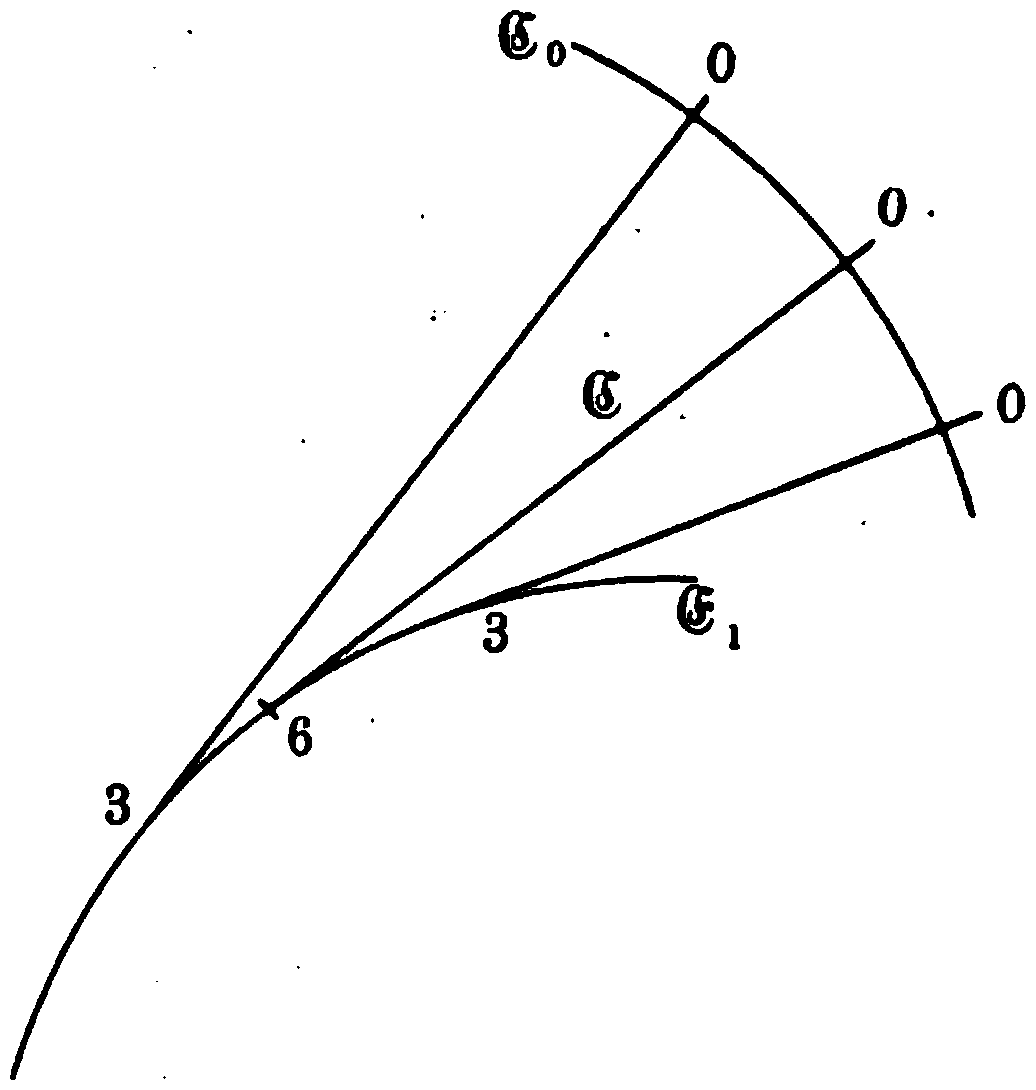
\includegraphics[width=\linewidth,height=38mm,keepaspectratio]{figures/fig12_accepted_derivative.png}
\end{minipage}\hfill
\begin{minipage}[c]{0.49\linewidth}\centering
\end{minipage}
\end{center}
\[
Dx=\frac{dx}{da}\,da=\left(\xi_a+\xi_t\frac{dt}{da}\right)da
=\frac{\xi_t\Delta_a-\xi_a\Delta_t}{-\Delta_t}\,da,
\]
\[
Dy=\frac{dy}{da}\,da=\left(\eta_a+\eta_t\frac{dt}{da}\right)da
=\frac{\eta_t\Delta_a-\eta_a\Delta_t}{-\Delta_t}\,da;
\]
由于 $\xi_t$ 与 $\eta_t$ 不同时消失，方程 (76) 可写成下列两种形式之一：
\[
\eta_a=\frac{\eta_t\xi_a}{\xi_t},\quad \xi_a=\frac{\xi_t\eta_a}{\eta_t}
\]
% src-pdfpage=0116
% src-break=0116
，由此可推出两个等式之一：
\begin{equation}\tag{78}
\begin{aligned}
Dy&=\frac{\eta_t}{\xi_t}\left(\xi_a+\xi_t\frac{dt}{da}\right)da=\frac{\eta_t}{\xi_t}Dx,\\
Dx&=\frac{\xi_t}{\eta_t}\left(\eta_a+\eta_t\frac{dt}{da}\right)da=\frac{\xi_t}{\eta_t}Dy
\end{aligned}
\end{equation}
。因此，在曲线 $\mathfrak{C}$ 上每个与 6 充分接近的点处，这条曲线都与场中具有同一 $a$ 值的极值曲线相切。故该曲线是场中极值曲线族的包络线；在上述假设下，包络线的存在性得证。

现在，沿曲线 $\mathfrak{C}$ 趋近属于 $a=a_0$ 的点 6；为此，使 $a$ 增加 $da$ 并假定
\begin{equation}\tag{79}
(a-a_0)da<0.
\end{equation}
。再若 $\xi_t$ 在点 6 不消失，并且
\begin{equation}\tag{80}
\xi_t\frac{dx}{da}\bigg|^6(a-a_0)<0,
\quad
\left|\frac{dx}{da}\right|^6>0,
\end{equation}
则在假设 (79) 下
\[
\xi_t\frac{dx}{da}\bigg|^6 da>0;
\]
所以，当量 $a-a_0$ 取关系 (80) 所规定的符号时，量 $\xi_t$ 与 $Dx$ 同号；沿曲线 $\mathfrak{C}$ 指向点 6 的前进方向，也就与相切极值曲线上 $t$ 增大的方向一致。把曲线 $\mathfrak{C}$ 上满足不等式 (80) 的那一半称为 $\mathfrak{C}_1$；沿此弧由 (78) 有
\begin{equation}\tag{81}
Dx=\alpha\xi_tdt=\alpha dx,
\quad
Dy=\alpha\eta_tdt=\alpha dy,
\end{equation}
其中 $\alpha$ 为正。这样的弧 $\mathfrak{C}_1$ 是否存在，只有在
\[
\frac{dx}{da}\bigg|^6=0,
\quad
\left.\xi_t\Delta_a-\xi_a\Delta_t\right|^6=0,
\]
时才有疑问；此时还有
\[
\Delta_t\frac{dy}{da}\bigg|^6=\eta_t\Delta_a-\eta_a\Delta_t
=\left.\eta_t\left(\Delta_a-\frac{\Delta_t\xi_a}{\xi_t}\right)\right|^6=0
\]
成立。于是，曲线 $\mathfrak{C}$ 可能在点 6 具有尖点（图~13）；只有当两个分支都从
% src-pdfpage=0117
% src-break=0117
点 6 沿着曲线 $\mathfrak{C}$ 上对应于 $t$ 增大的方向前进时，才不存在弧 $\mathfrak{C}_1$。我们把这称为例外情形。

% unit: fig13 source=kneser_lvr_1900_archiveorg.pdf#p0117 authorial=true type=hq_sourcecrop
\begin{center}
{\small 图~13.}\par\vspace{1mm}
\begin{minipage}[c]{0.47\linewidth}\centering
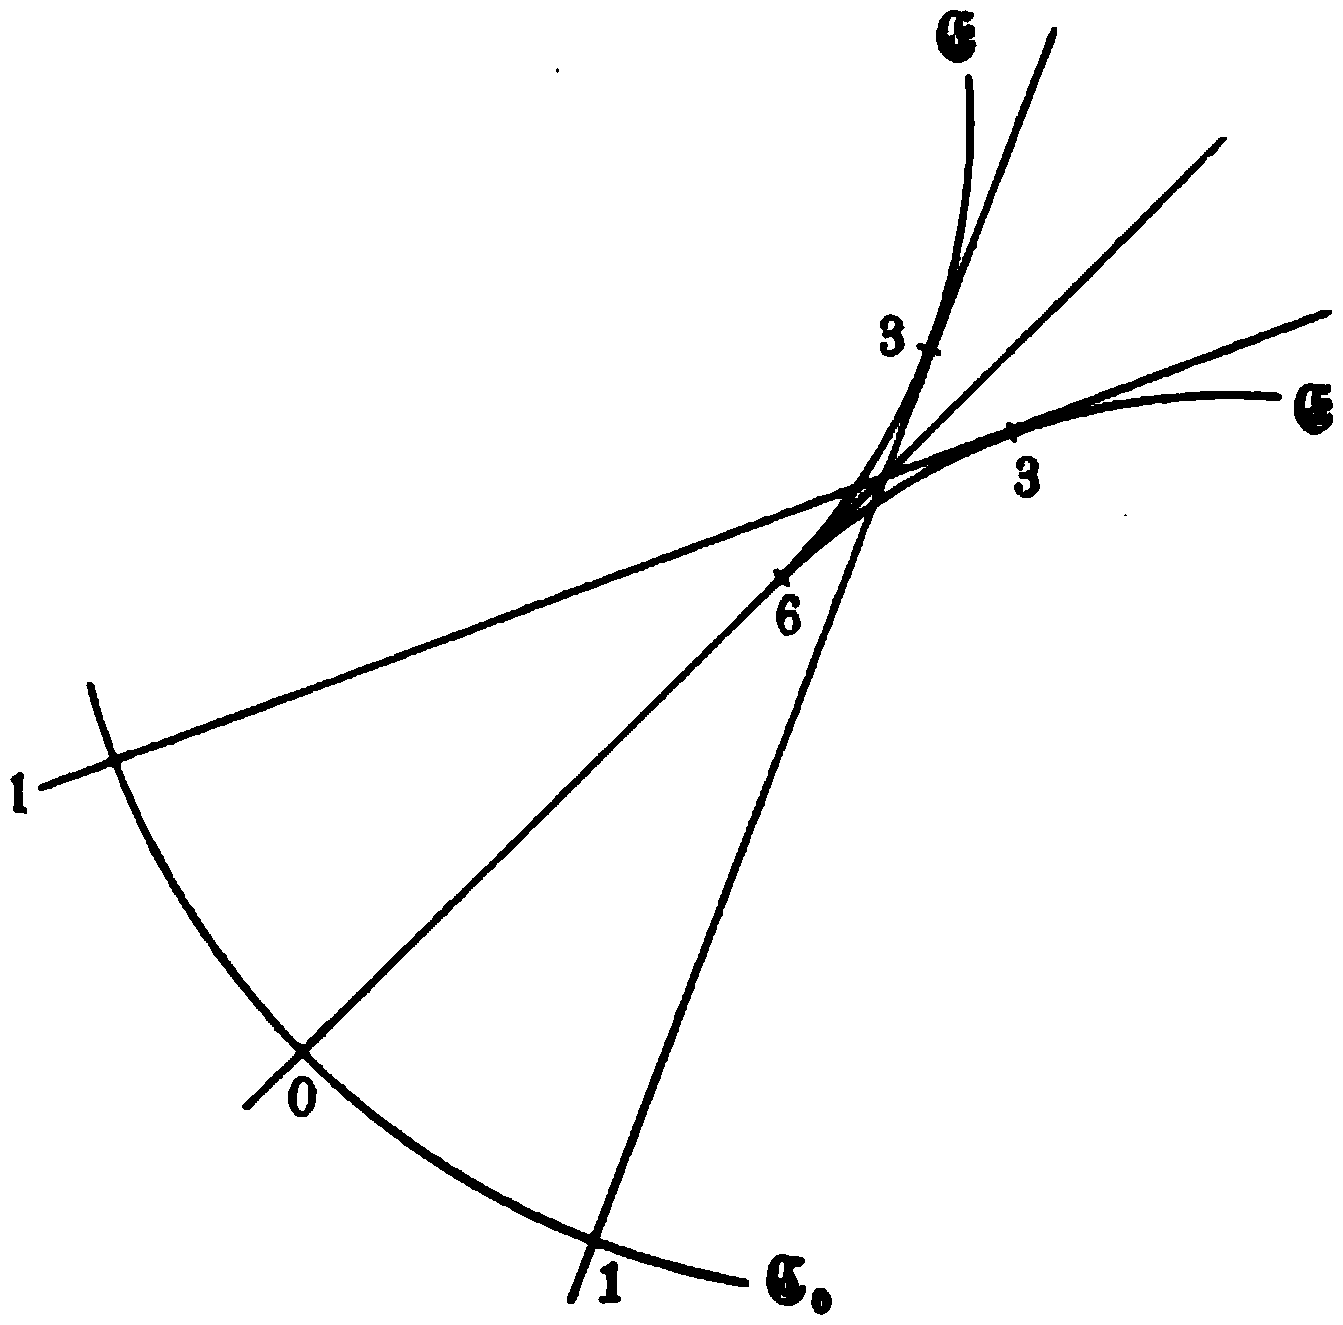
\includegraphics[width=\linewidth,height=38mm,keepaspectratio]{figures/fig13_accepted_derivative.png}
\end{minipage}\hfill
\begin{minipage}[c]{0.49\linewidth}\centering
\end{minipage}
\end{center}

仍设 0 是曲线 $\mathfrak{C}_0$ 上的一点，3 是场中同一条极值曲线上的另一点，并以 $a$ 与 $t$ 为其参数。于是量
\[
u=\overline{J}_{03}=\int_0^3F(\xi,\eta,\xi_t,\eta_t)dt
\]
不仅如我们已知的那样在场内，而且在区域 $\mathfrak{B}'$ 内也是 $a$ 与 $t$ 的正则函数；在该区域内，量 $\xi,\eta,F(\xi,\eta,\xi_t,\eta_t)$ 保持正则。方程
\[
\frac{\partial u}{\partial a}=F_{x'}(\xi,\eta,\xi_t,\eta_t)\xi_a
+F_{y'}(\xi,\eta,\xi_t,\eta_t)\eta_a,
\]
\[
\frac{\partial u}{\partial t}=F(\xi,\eta,\xi_t,\eta_t),
\]
最初虽是在场内导出的，但在区域 $\mathfrak{B}'$ 内同样成立，因为方程的两端在该区域内都保持为 $a$ 与 $t$ 的正则函数。特别令 3 为曲线 $\mathfrak{C}$ 上的一点，则沿该曲线前进时有
\[
\begin{aligned}
du={}&F_{x'}(\xi,\ldots,\eta_t)(\xi_a da+\xi_tdt)
+F_{y'}(\xi,\ldots,\eta_t)(\eta_ada+\eta_tdt)\\
={}&F_{x'}(\xi,\ldots,\eta_t)Dx+F_{y'}(\xi,\ldots,\eta_t)Dy.
\end{aligned}
\]
另一方面，沿曲线 $\mathfrak{C}$ 作积分
\[
J_{36}=\int_3^6F(x,y,Dx,Dy),
\]
并使符号 $D$ 对应于沿曲线 $\mathfrak{C}$ 指向点 6 的运动。于是
\[
dJ_{36}=-F(x,y,Dx,Dy)=-F(\xi,\eta,Dx,Dy).
\]
若能应用齐次性方程，这个量便与上面为 $du$ 得到的量互为相反数：
% src-pdfpage=0118
% src-break=0118
\[
F_{x'}(\xi,\eta,\xi_t,\eta_t)=F_{x'}(\xi,\eta,Dx,Dy),
\]
\[
F_{y'}(\xi,\eta,\xi_t,\eta_t)=F_{y'}(\xi,\eta,Dx,Dy)
\]
。也就是说，当方程 (81) 成立且 $\alpha$ 为正，从而点 3 属于弧 $\mathfrak{C}_1$ 时，有
\[
\begin{aligned}
F_{x'}(\xi,\ldots,\eta_t)Dx+F_{y'}(\xi,\ldots,\eta_t)Dy
={}&F_{x'}(\xi,\eta,Dx,Dy)Dx\\
&+F_{y'}(\xi,\eta,Dx,Dy)Dy\\
={}&F(\xi,\eta,Dx,Dy),
\end{aligned}
\]
\[
du+dJ_{36}=d(\overline{J}_{03}+J_{36})=0.
\]
当点 3 与 6 的距离成为无穷小时，极值曲线 03 与 $\mathfrak{C}$ 重合，显然有
\[
\lim(\overline{J}_{03}+J_{36})=\overline{J}_{06}
\]
，所以一般地
\begin{equation}\tag{82}
\overline{J}_{03}+J_{36}=\overline{J}_{06}.
\end{equation}
若曲线 $\mathfrak{C}$ 缩为点 6，则显然得到
\[
J_{36}=0.
\]
因此，场中不同极值曲线上的 $\overline{J}_{06}$ 具有相同的值。

现在，由极值弧 03 与曲线 $\mathfrak{C}_1$ 上的弧段 36 组成的曲线 036，可以看作属于弧 06 的较小邻域。事实上，一旦距离 36 充分小，弧 36 的切线与点 6 处的切线任意接近；极值曲线 03 连续趋于弧 06，其切线也与后者的切线任意接近。因此，曲线 036 属于这样一类曲线 $\Omega$：若弧 06 哪怕只使积分 $J$ 取得弱极值，比较对象就必须包括连接曲线 $\mathfrak{C}_0$ 与点 6 的其他曲线，也就必须包括曲线 036。此时差
\[
J_{06}-J_{036}=J_{06}-(J_{03}+J_{36})
\]
本应具有固定符号而不消失，但依 (82)，它的值为零。所以极值弧 06 肯定不能使积分 $J$ 取得极值，连弱极值也不能；极值恰在点 6 处以方程 (82) 所更精确描述的方式终止。假定场存在，我们由此证明了下列结果。

% src-pdfpage=0119
% src-break=0119
若正则曲线 $\mathfrak{C}_0$ 在点 0 被极值曲线 $\mathfrak{C}$ 横截，而点 5 沿后一曲线运动，则弧 05 不再使积分 $J$ 取得弱极值——比较对象是从点 5 通向曲线 $\mathfrak{C}_0$ 的各条曲线——一旦点 5 移入曲线 $\mathfrak{C}_0$ 的焦点。若曲线 $\mathfrak{C}_0$ 缩为点 0，则当点 5 移至与 0 共轭的点时，对于连接固定点 0 与 5 的曲线，也有同一结论。唯一的例外是：场中曲线必然存在的包络线在焦点处有一种特殊的尖点；在这种情形下，上述考察表明，在由两个共轭点限定的极值曲线段的任意邻域内，都有另一些极值曲线段与它具有共同的起点，并且必定不再给出极值。例如，在图~13 中显然有
\[
\overline{J}_{13}=\overline{J}_{06}+J_{63}.
\]

% unit: sec26 source=kneser_lvr_1900_archiveorg.pdf#p0119 authorial=true
\begin{center}{\large \S~26.}\end{center}

\noindent\textbf{例。} 对质点作直线弹性振动时，哈密顿原理导出积分
\[
J=\int dx\,(p^2-y^2),
\]
其极值曲线由简单方程
\[
\frac{dp}{dx}+y=0
\]
确定。极值曲线
\[
y=a\sin x
\]
全都通过固定点 $0\ (x=y=0)$；我们把曲线 $\mathfrak{C}_0$ 看作缩在该点。置 $a=t$，得到
\[
\Delta=\frac{\partial(x,a\sin x)}{\partial(x,a)}=\sin x;
\]
因此，与点 0 共轭的点 6 满足 $x=\pi$；在它的邻域内，$x$ 与 $a\sin x$ 显然都是正则函数。曲线 $\mathfrak{C}$ 缩在点 6，因为所考察曲线族的全部极值曲线
% src-pdfpage=0120
% src-break=0120
都通过该点。沿这些曲线得到的积分 $J$ 具有相同的值：
\[
J_{06}=\int_0^\pi a^2dx(\cos^2x-\sin^2x)
=\frac{a^2\sin2x}{2}\bigg|_0^\pi=0.
\]
球面大圆作为最短线时也出现同一情形：与每一点共轭的是其对径点。在三轴椭球面上，从一个脐点出发的测地线中，与该起点共轭的是直径对面的脐点；连接二者的各条测地弧长度相等。

一般方程 (82) 最简单的例子，是渐屈线的一项基本性质：渐伸线上分别对应于渐屈线弧两端的曲率半径之差，等于该段渐屈线弧的长度。把方程 (82) 应用于问题 I，并把渐伸线看作曲线 $\mathfrak{C}_0$，即可得到这个定理。

\noindent\textbf{问题 VI（\S~11）。} 中心位于 $x$ 轴上且横坐标为 $x_0$ 的相似变换，由方程
\[
\bar y=\alpha y,
\quad
\bar x-x_0=\alpha(x-x_0),
\quad
\bar x=\alpha x-(\alpha-1)x_0
\]
定义。因此，若方程
\[
y=\frac{a(1+p^2)^2}{2p^3},
\quad
x=b+\frac{a}{2}\left(\frac{3}{4p^4}+\frac{1}{p^2}+\lg p\right)
\]
表示一条极值曲线，则点 $(\bar x,\bar y)$ 也描出一条极值曲线。若以 $X,Y$ 为流动坐标，这种极值曲线的任一切线方程为
\[
Y-y=p(X-x),
\]
所以它与 $x$ 轴相交于一点 $T$，该点的横坐标为
\[
X=x-\frac{y}{p}
\]
。又因为
\[
\frac{dX}{dp}=\frac{y}{p^2},
\]
而 $p=0,p=+\infty$ 分别使 $X$ 取相应值 $-\infty,+\infty$，所以点 $T$ 在 $a$、从而 $y$ 为正时，沿 $x$ 轴按正方向恰好走过一次，只要
% src-pdfpage=0121
% src-break=0121
$p$ 递增地取遍一切正值；此时所考察切线的切点也就遍历整条曲线（\S~11）。

现在，设一直线 $\mathfrak{C}_0$ 以锐角 $\psi$ 倾向于 $+x$ 轴（图~14）。当极值曲线 $\mathfrak{C}$ 在点 0 满足
\[
\tg\psi=\frac{2p}{3+p^2}=\frac{p}{1+\frac12(1+p^2)}
\]
时，它在该点横截这条直线；这个方程显然给出
\begin{equation}\tag{83}
\tg\psi<p
\end{equation}
。一个给定的 $\tg\psi$ 值对应两个实数 $p$ 值，其乘积为 3，只要不等式
\[
\tg\psi<\frac1{\sqrt3},\quad \psi<30^\circ
\]
成立；我们用其中一个值来构造 $\mathfrak{C}$，这个值小于 $\sqrt3$，并对应于极值曲线的这样一个分支：该分支的各弧段使阻力取得最小值（\S~18）。再设 7 是极值曲线在点 0 处的切线与 $x$ 轴的交点，8 是该轴与直线 $\mathfrak{C}_0$ 的交点。由 (83)，点 7 位于 8 的右侧，即正方向一侧。因此，当一点从 0 出发，沿所构造的极值曲线 $\mathfrak{C}$ 按 $x$ 增大、也就是 $p$ 减小的方向运动时，点 $T$ 从位置 7 向 $-\infty$ 移动，中途必到达位置 8。设经过 8 的曲线 $\mathfrak{C}$ 的切线，其切点为 6。

% unit: fig14 source=kneser_lvr_1900_archiveorg.pdf#p0121 authorial=true type=hq_sourcecrop
\begin{center}
{\small 图~14.}\par\vspace{1mm}
\begin{minipage}[c]{0.47\linewidth}\centering
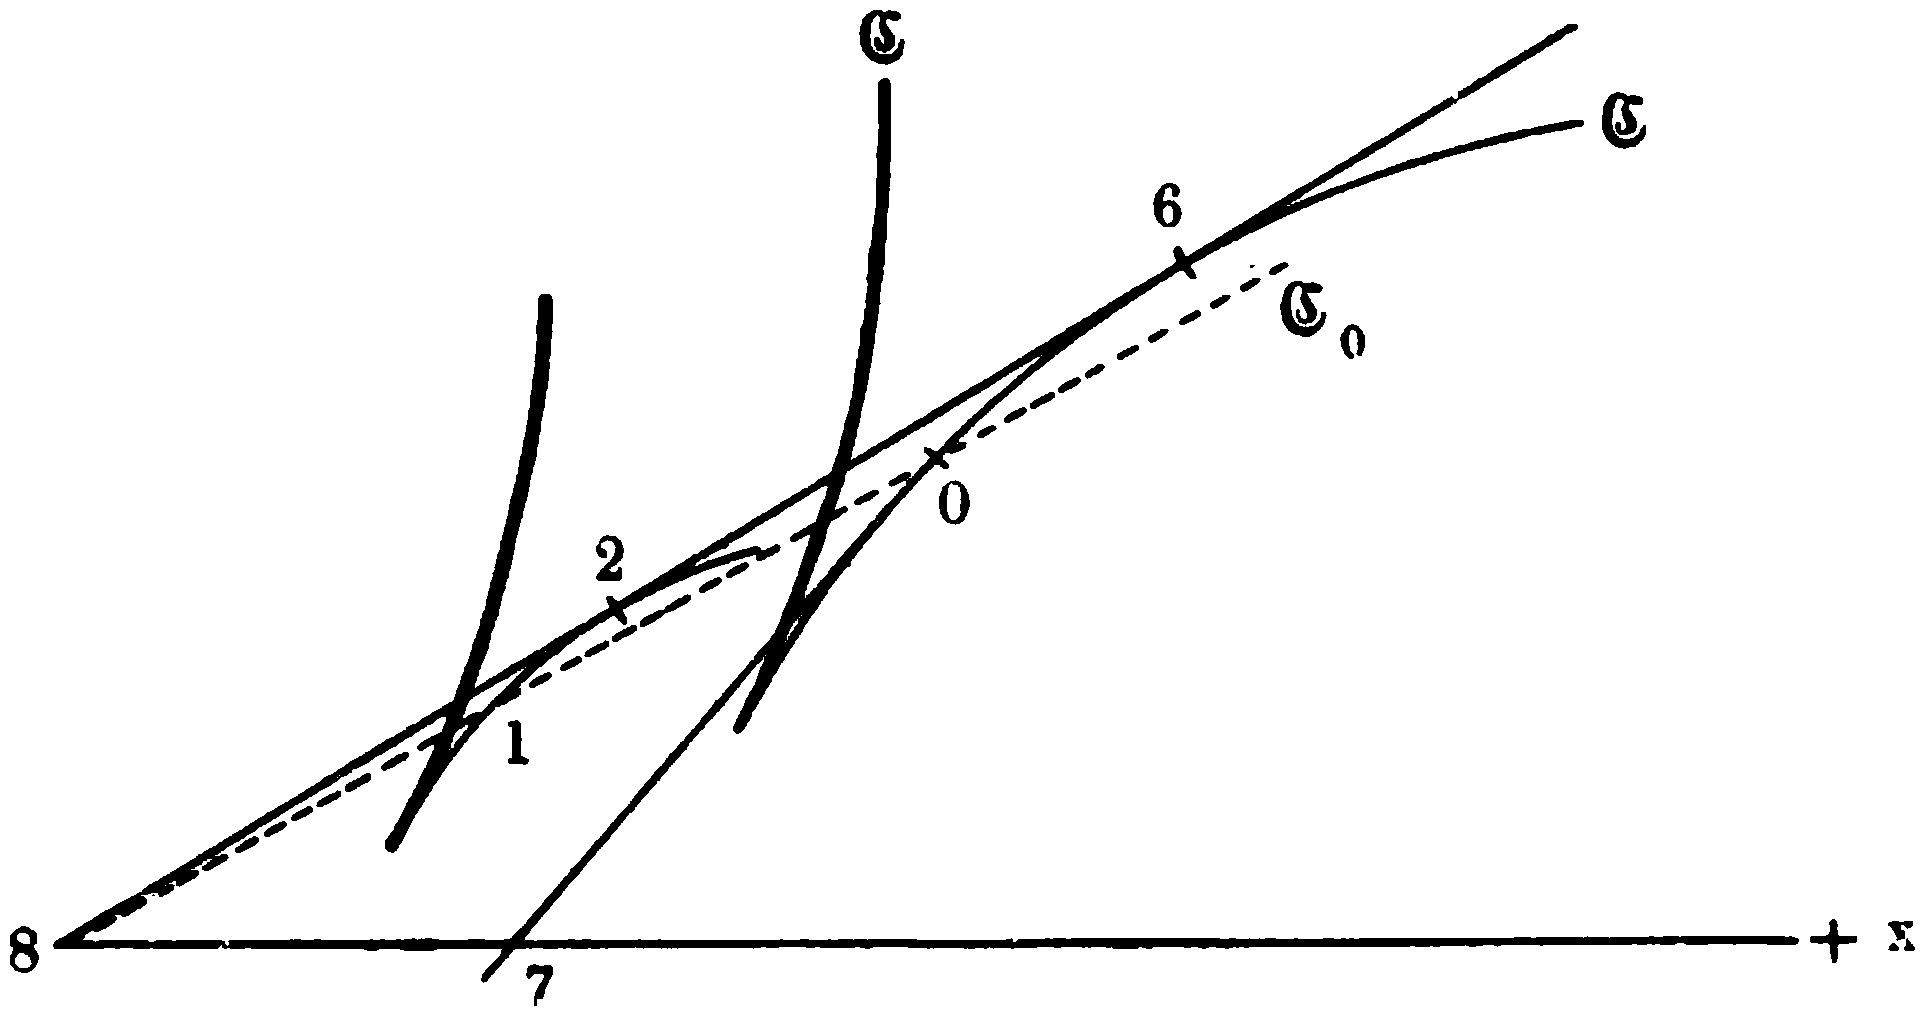
\includegraphics[width=\linewidth,height=36mm,keepaspectratio]{figures/fig14_accepted_derivative.png}
\end{minipage}\hfill
\begin{minipage}[c]{0.49\linewidth}\centering
\end{minipage}
\end{center}

现在以点 8 为一族相似变换的中心；这些变换把曲线 $\mathfrak{C}$
% src-pdfpage=0122 portion=upper
% src-break=0122
变成一族横截直线 $\mathfrak{C}_0$ 且与切线 68 相切的极值曲线。因此，切线 68 就是一般理论中的包络线 $\mathfrak{C}$，6 是直线 $\mathfrak{C}_0$ 在曲线 $\mathfrak{C}$ 上的焦点，而 $\mathfrak{C}_1$ 是线段 68。若 2 是该线段上的任一点，而所构造曲线族中在点 2 与之相切的极值曲线与直线 $\mathfrak{C}_0$ 相交于点 1，则阻力积分满足
\[
\overline{J}_{12}+J_{26}=\overline{J}_{06},
\]
其中 $J_{26}$ 沿直线 68 计算。因此，若点 5 沿曲线 $\mathfrak{C}$ 运动，则只要点 5 属于弧 06，弧 05 就相对于从点 5 引向直线 $\mathfrak{C}_0$ 的曲线，使阻力取得弱最小值；当点 5 移入位置 6 时，上式表明弧 06 已以何种方式丧失最小值性质。

问题 VI 中用来构造并限定一个场的方法，可以推广到任何这样的问题：一族极值曲线在某个已知连续变换群的作用下彼此变换。变换的所谓轨道曲线与该族极值曲线相切之处，就是场的边界。


% machine-unit: sec27 source=kneser_lvr_1900_archiveorg.pdf#p0122 authorial=true
% src-pdfpage=0122 portion=lower
% src-break=0122
\begin{center}{\large \S~27.}\end{center}

在各个具体问题中，极值曲线至少可以分段地被场所包围，这通常很容易看出。但为了对这种关系建立一般定理，我们要作一项具有一般性质的函数论考察；以后还会用到它。

在微分方程
\begin{equation}\tag{84}
\frac{dy}{dx}=f(x,y,z,\ldots),\quad
\frac{dz}{dx}=g(x,y,z,\ldots),\ldots,
\end{equation}
中，设方程的个数为 $n$，并与未知量 $y,z,\ldots$ 的个数相同；再设各右端在点
\begin{equation}\tag{85}
x=x_0,\quad y=Y_0,\quad z=Z_0,\ldots;
\end{equation}
% src-pdfpage=0123
% src-break=0123
的邻域内都是正则的。众所周知，存在一个积分组，其各成员在 $x=x_0$ 时取任意指定的值
\[
y=y_0,\quad z=z_0,\ldots
\]
，只要量
\[
|y_0-Y_0|,\quad |z_0-Z_0|,\ldots
\]
低于某个界。为求这些积分的级数，可将方程 (84) 对 $x$ 微分，并在右端消去各微商，把一切都表示为仅含 $x,y,z,\ldots$ 的函数。在所得表达式中——它们在点 (85) 也都是正则的——对 $x,y,z,\ldots$ 代入数值 $x_0,y_0,z_0,\ldots$，便得到这些特定解 $y,z,\ldots$ 关于 $x-x_0$ 的泰勒展开系数。正如积分存在性证明所示，这些系数的绝对值小于变量 $x-x_0$ 的某个收敛幂级数的相应系数，而该幂级数与量 $y_0,z_0,\ldots$ 的具体选择无关。因此，若把后面这些量看作变量，则所得的 $y,z,\ldots$ 级数在某个区域内一致收敛；对某个给定参数 $x$，它们的值因而可表示成 $y_0-Y_0,z_0-Z_0,\ldots$ 的幂级数。显然可置
\[
\begin{aligned}
y&=y_0+(x-x_0)[x-x_0,y_0-Y_0,z_0-Z_0,\ldots]_0,\\
z&=z_0+(x-x_0)[x-x_0,y_0-Y_0,z_0-Z_0,\ldots]_0,\ldots,
\end{aligned}
\]
从而函数行列式
\[
\frac{\partial(y,z,\ldots)}{\partial(y_0,z_0,\ldots)}
\]
在 $x=x_0$ 时取值 $1$。所以，$y,z,\ldots$ 在任一给定参数 $x$ 时的值，作为量 $y_0,z_0,\ldots$ 的函数彼此独立。

现在，设量 $Y,Z,\ldots$ 定义为 $x$ 的正则函数，并在一个实区间 $\mathfrak J$ 上满足方程 (84)；该区间的下端为 $x_0$。设在此处
\[
Y=Y_0,\quad Z=Z_0,\ldots,
\]
而在 $x=x_1$ 处
\[
Y=Y_1,\quad Z=Z_1,\ldots,
\]
并且区间 $\mathfrak J$ 中得到的每个数值组 $(x,Y,Z,\ldots)$，都属于函数 $f,g,\ldots$
% src-pdfpage=0124
% src-break=0124
保持正则的某个邻域。由上述论证，存在正数 $\delta,\varepsilon$，使得在区间
\begin{equation}\tag{86}
x_0\leq x\leq x_0+\varepsilon
\end{equation}
上有一个正则积分组；若 $x_1$ 是该区间的任一点，并且不等式
\[
|y_1-Y_1|<\delta,\quad |z_1-Z_1|<\delta,\ldots
\]
成立，则该积分组在 $x=x_1$ 时取指定值 $y_1,z_1,\ldots$。在区间 (86) 的任一给定位置，$y,z,\ldots$ 的值在数值组 $(Y_1,Z_1,\ldots)$ 的邻域内，都是 $y_1,z_1,\ldots$ 的彼此独立的正则函数。再令 $\gamma$ 为一切可能的 $\varepsilon$ 值的上确界；那么量
\[
\bar x=x_0+\gamma
\]
不可能位于区间 $\mathfrak J$ 的内部。否则，可以选取正数 $\bar\varepsilon,\bar\delta$，使得对区间
\begin{equation}\tag{87}
-\bar\varepsilon<x-\bar x<\bar\varepsilon
\end{equation}
，量 $\bar\delta$ 具有量 $\delta$ 对区域 (86) 所具有的同一意义。但区域 (86) 可以任意接近点 $\bar x$，所以其中存在同时属于区域 (87) 的点 $x_1$。令 $\delta_1$ 为 $\delta,\bar\delta$ 中较小者，并假定
\[
|y_1-Y_1|<\delta_1,\quad |z_1-Z_1|<\delta_1,\ldots,
\]
则每个满足这些不等式的数值组 $y_1,z_1,\ldots$ 都确定一个积分组；这个积分组在两个区域 (86)、(87)，因而在整个区域
\[
x_0\leq x<\bar x+\bar\varepsilon
\]
内正则，并且其在任一给定位置的值都是量 $y_1,z_1,\ldots$ 的彼此独立的正则函数。因此，若置
\[
\varepsilon_1=\gamma+\bar\varepsilon,\quad \bar x+\bar\varepsilon=x_0+\varepsilon_1,
\]
则对于区域
\[
0\leq x-x_0<\varepsilon_1
\]
，量 $\delta_1$ 将具有量 $\delta$ 对区域 (86) 所具有的同一意义；但这与上确界的定义矛盾，因为 $\varepsilon_1>\gamma$。因此，一切 $x_0+\varepsilon$ 值的上确界位于
% src-pdfpage=0125 portion=upper
% src-break=0125
区间 $\mathfrak J$ 之外或其边界上。所以，区间 (86) 可以换成任何从 $x_0$ 出发并任意接近区间 $\mathfrak J$ 边界的区间。

这就表明，积分流形 $(x,Y,Z,\ldots)$ 可以按如下方式被邻近的积分流形所包围。存在积分
\[
y=\Phi(x,a,b,\ldots,k),\quad z=\Psi(x,a,b,\ldots,k),\ldots,
\]
其中含有 $n$ 个常数 $a,b,\ldots,k$；当它们取某个特定数值组
\[
a=A,\quad b=B,\ldots,\quad k=K
\]
时，这些积分变成 $Y,Z,\ldots$。此外，这些积分还是其 $n+1$ 个参数的正则函数，只要 $x$ 位于区间 $\mathfrak J$ 的内部，而差
\[
|a-A|,\quad |b-B|,\ldots,\quad |k-K|
\]
充分小。在这些假设下，函数行列式
\[
\frac{\partial(\Phi,\Psi,\ldots)}{\partial(a,b,\ldots)}
\]
不为零。

% machine-unit: sec28 source=kneser_lvr_1900_archiveorg.pdf#p0125 authorial=true
\begin{center}{\large \S~28.}\end{center}

在积分
\[
J+\Delta J=\int F(x+\delta x,y+\delta y,x'+\delta x',y'+\delta y')\,dt
\]
中，把被积函数展开成泰勒级数，则各变分的全部二次项的两倍之和的积分为
\[
\int dt\{F_{xx}\delta x^2+2F_{xy}\delta x\delta y+\cdots+F_{x'x'}\delta x'^2+\cdots\}.
\]
这个表达式可由变分
\[
\delta J=\int(F_x\delta x+F_y\delta y+F_{x'}\delta x'+F_{y'}\delta y')\,dt,
\]
按微分法则施行运算 $\delta$ 得到；施行该运算时，把 $t,\delta x,\delta x',\delta y,\delta y'$ 看作相对于它的常数。因此，将上述表达式记作 $\delta^2J$，并称为 $J$ 的第二变分。若变分 $\delta x,\delta y$ 含有常因子 $\varepsilon$，则显然
\begin{equation}\tag{88}
\Delta J=\delta J+\frac12\delta^2J+[\varepsilon]_3,
\end{equation}
% END PHYSICALLY EMBEDDED BODY INH03 1/5
% BEGIN PHYSICALLY EMBEDDED BODY INH03 2/5: inherited/INH03_pdf101_150_producer_r3_fraktur/work/zh_126_131.tex
% src-pdfpage=0126
% src-break=0126
而且 $\delta^2J$ 含有因子 $\varepsilon^2$。现在可以写成：
\[
\delta J=F_{x'}\delta x+F_{y'}\delta y+
\int dt(P\delta x+Q\delta y),
\]
由于符号 $\delta$ 可以同关于 $t$ 的积分符号互换，因而有
\[
\delta^2J=\delta F_{x'}\delta x+\delta F_{y'}\delta y+
\int dt(\delta P\delta x+\delta Q\delta y),
\]
这个公式很容易用计算加以验证。特别地，在
\[
\left.\delta x\right|^0=\left.\delta x\right|^1=
\left.\delta y\right|^0=\left.\delta y\right|^1=0
\]
的情形，得到
\[
\delta^2J_{01}=\int_0^1dt(\delta P\delta x+
\delta Q\delta y).
\]

把这个公式应用于由方程
\[
\delta x=\omega X,
\quad
\delta y=\omega Y
\]
所定义的法向变分；其中 $X,Y$ 的意义同第~24~节，而 $\omega$ 在位置 0 和 1 处消失。于是根据那里导出的恒等式 (75)，
\begin{equation}\tag{89}
\delta^2J_{01}=\int_0^1\omega(X\delta P+Y\delta Q)\,dt
=\int_0^1\omega\left(F_2\omega-\frac{d(F^1\omega')}{dt}\right)dt
\end{equation}
或者，经分部积分后，
\begin{equation}\tag{90}
\delta^2J_{01}=\int_0^1dt\,(F^1\omega'^2+F_2\omega^2).
\end{equation}

现在再设 0 和 6 是共轭点，而弧 02 延伸到后一个点以外。于是根据第~24~节，方程
\begin{equation}\tag{91}
F_2\omega-\frac{d(F^1\omega')}{dt}=0
\end{equation}
有一个在点 0 和 6 处消失、并在点 6 处变号的积分；把弧 02 取得适当，使 0 和 6 是这个积分 $\omega$ 在该弧上仅有的两个零点。若 $\varepsilon$ 是充分小的常数，并且 $F^1$ 沿整个弧 02 不为零，则方程
\[
(F_2-\varepsilon)w-\frac{d(F^1w')}{dt}=0
\]
根据第~27~节有一个积分；它同 $\omega$ 一样在区间 02 上正则，并满足方程
% src-pdfpage=0127
% src-break=0127
\[
\left.w\right|^0=\left.\omega\right|^0=0
\]
而且在 0 与 2 之间同样只有一个零点 7；当 $\varepsilon=0$ 时，这个零点同 6 重合。于是，对于法向变分
\[
\delta x=Xw\alpha,
\quad
\delta y=Yw\alpha,
\]
其中 $\alpha$ 为常数，根据一般公式 (89) 有
\[
\delta^2J_{07}=\alpha^2\int_0^7 w\left(F_2w-\frac{d(F^1w')}{dt}\right)dt
=\alpha^2\varepsilon\int_0^7w^2dt.
\]
因此，若在区间 72 上令
\[
\delta x=\delta y=0,
\]
那么，由于 $\varepsilon$ 充分小时点 7 位于区间 02 的内部，便有
\[
\delta^2J_{02}=\delta^2J_{07}=\alpha^2\varepsilon\int_0^7\omega^2dt,
\]
又因为变分后的曲线是一条极值曲线，根据 (88) 有
\[
\delta J_{02}=0,
\quad
\Delta J_{02}=\frac12\delta^2J_{07}+[\alpha]_3
=\frac{\alpha^2\varepsilon}{2}\int_0^7w^2dt+[\alpha]_3.
\]
显然，只要 $\alpha$ 足够小，这个量就同 $\varepsilon$ 具有相同符号，因而既可为正也可为负；所以弧 02 肯定不使积分 $J$ 取得极值。

这一论证的基本思想源于埃尔德曼和魏尔斯特拉斯。它同第~24、25~节所给论证的区别在于：后者一般已经证明，由两个共轭点限定的弧不可能给出极值，但须排除一个例外情形；刚才的推导也适用于这个例外情形，却始终要求所考察的弧越过其起点的共轭点。

如果弧 01 不含一对共轭点，而且 $F^1$ 在该弧上不消失，则公式 (90) 表明，第二变分的符号同量 $F_1$ 或 $F^1$ 的符号一致。事实上，若 $u$ 在 $t_0$ 至 $t_1$ 之间是 $t$ 的正则函数，则显然有
\[
\int_0^1(u'\omega^2+2u\omega\omega')\,dt
=\int_0^1\frac{d}{dt}(u\omega^2)\,dt
=u\omega^2\bigg|_0^1=0,
\]
% src-pdfpage=0128
% src-break=0128
\begin{equation}\tag{92}
\delta^2J_{01}=\int_0^1dt\,[F^1\omega'^2+2u\omega\omega'+(F_2+u')\omega^2],
\end{equation}
并且，这个表达式中的被积式同 $F_1$ 具有相同符号，只要 $u$ 能按照方程
\begin{equation}\tag{93}
(F_2+u')F^1-u^2=0
\end{equation}
加以确定；这时简单地有
\begin{equation}\tag{94}
\delta^2J_{01}=\int_0^1F^1\left(\omega'+\frac{u\omega}{F^1}\right)^2dt.
\end{equation}
但方程 (93) 同任何形如
\[
u'=Lu^2+Mu+N
\]
的方程一样，可以化为一个二阶线性微分方程。令
\[
u=-\frac1L\frac{\omega'}{\omega},
\]
便得到
\[
\omega''-\left(M+\frac{L'}L\right)\omega'+LN\omega=0;
\]
从方程 (93) 出发，以这种方式恰好得到方程 (91)，而量 $\Delta(t,a):\sqrt{\xi_t^2+\eta_t^2}$ 满足这个方程。在所作假设下，这个量沿弧 01 不为零，因而给出一个在积分区间内正则的量 $u$：
\[
u=-\frac{F_1\sqrt{\xi_t^2+\eta_t^2}}{\Delta(t,a)}\frac{d}{dt}\left(\frac{\Delta(t,a)}{\sqrt{\xi_t^2+\eta_t^2}}\right).
\]
因此，如果已知一个极值曲线族，那么对于一段具有上述性质的弧和一个法向变分，公式 (94) 可以显式地写出。

为了证明，相对于所有由 $\mathfrak C$ 通过法向变分得到并且属于一个较窄邻域的曲线，极值确实出现，只须把方程 (93) 替换为下式，其中 $\varepsilon$ 表示一个充分小的常数：
\[
(F_2+u')F^1-u^2=\varepsilon^2.
\]
根据第~27~节，当 $\varepsilon$ 足够小时，这个方程同原方程一样有一个在 0 至 1 之间正则的积分。把这个积分代入公式 (92)，积分号下的二次型便是定号的，而公式
% src-pdfpage=0129 portion=upper
% src-break=0129
\[
\Delta J_{01}=\frac12\delta^2J_{01}+\int_0^1[\omega,\omega']_3\,dt
\]
很容易表明极值确实出现。

% machine-unit: sec29 source=kneser_lvr_1900_archiveorg.pdf#p0129 authorial=true
\begin{center}{\large \S~29.}\end{center}

设 02 是任意曲线段，并且它在每一点的邻域内都是正则的（第~1~节）。那么沿此曲线段，$x$ 和 $y$ 总能表示为某个参数 $t$ 的正则单值函数，例如可取从 0 向 2 测量的弧长为参数。该弧长由方程
\[
\frac{dt}{dx}=\sqrt{1+\left(\frac{dy}{dx}\right)^2},
\quad
\frac{dt}{dy}=\sqrt{1+\left(\frac{dx}{dy}\right)^2}
\]
定义；在沿 02 的方向前进时，每个平方根都取同其分母中位于根号下的微分相同的符号。事实上，若在位置 1 处量 $dy:dx$ 有限，因而 $y$ 是 $x$ 的正则函数，则 $\frac{dt}{dx}$ 也具有同样性质，而且这个量不为零：
\[
\frac{dt}{dx}=\left.\frac{dt}{dx}\right|^1+[x-x_1]_1,
\quad
t-t_1=\left.\frac{dt}{dx}\right|^1(x-x_1)+[x-x_1]_2;
\]
但第二个方程给出
\[
x-x_1=[t-t_1]_1,
\]
因此 $x$ 和 $y$ 在位置 1 处是 $t$ 的正则函数。当然，如果 $dx:dy$ 有限，因而 $x$ 可表示为 $y$ 的正则函数，通过类似展开也得到同一结果。关于平方根符号的规定使得沿 02 的方向前进时 $dt$ 总为正，因此不同的 $t$ 值对应弧上的不同点。

现在若弧 02 是一条极值曲线的一部分，并且只定义了这样的数值组 $(x,y,x',y')$：被积函数 $F$ 在这些数值组的邻域内正则，那么方程
\[
x'^2+y'^2=1,
\quad
F_1=F^1,
\quad
F_x-F_{x'}'=F_y-F_{y'}'=0,
\]
成立；由此导出两个等价的方程组：
\begin{equation}\tag{95}
\begin{aligned}
F_x-F_{x'x}x'-F_{x'y}y'-F_{x'x'}x''-F_{x'y'}y''&=0,\\
x'x''+y'y''&=0;
\end{aligned}
\end{equation}
% src-pdfpage=0130
% src-break=0130
\begin{equation}\tag{96}
\begin{aligned}
F_y-F_{y'x}x'-F_{y'y}y'-F_{y'x'}x''-F_{y'y'}y''&=0,\\
x'x''+y'y''&=0.
\end{aligned}
\end{equation}
从每个方程组都可将 $x'',y''$ 算作 $x,y,x',y'$ 的函数；它们表现为分式，分子是沿弧 02 关于 $t$ 的正则函数，分母则是行列式
\[
\begin{vmatrix}
F_{x'x'}&F_{x'y'}\\
x'&y'
\end{vmatrix},
\quad
\begin{vmatrix}
F_{y'x'}&F_{y'y'}\\
x'&y'
\end{vmatrix}
\]
考虑到第~16~节导出的恒等式，它们可以化为如下形式：
\[
F_1y'(x'^2+y'^2)=F_1y'=\frac{\bar f_{qq}}{y'^2},
\quad
F_1x'(x'^2+y'^2)=F_1x'=\frac{f_{pp}}{x'^2}.
\]
因此，我们再次引入第~17~节中的限制：对于弧 02 的每个线元，量 $F_1$ 均不为零；这可能排除方程 (95)、(96) 的某些奇解。于是，无论以方程组 (95) 还是 (96) 为基础，都可得到 $x''$ 和 $y''$ 的表达式；这些表达式在弧 02 的一个线元所定义的每个数值组 $(x,y,x',y')$ 的邻域内都是正则的。把这些表达式记为
\[
\frac{dx'}{dt}=M(x,y,x',y'),
\quad
\frac{dy'}{dt}=N(x,y,x',y')
\]
并添上方程
\[
\frac{dx}{dt}=x',
\quad
\frac{dy}{dt}=y'
\]
其右端总是正则的，便得到一个具有第~27~节所考察性质的方程组；其中 $x$ 已由 $t$ 代替，而区间 $\mathfrak J$ 从 $t_0$（即 0）延伸到 $t_2$。因此存在一个形如
\begin{equation}\tag{97}
x=X(t,a,b,\alpha,\beta),
\quad
y=Y(t,a,b,\alpha,\beta),
\end{equation}
的积分组；其中函数 $X,Y$ 是正则的，只要 $t$ 属于指定区间，而且各差
\[
|a-x_0|,
\quad
|b-y_0|,
\quad
|\alpha-x'_0|,
\quad
|\beta-y'_0|
\]
充分小；同时恒等式
\begin{equation}\tag{98}
\begin{aligned}
X(0,a,b,\alpha,\beta)&=a,
&X_t(0,a,b,\alpha,\beta)&=\alpha,\\
Y(0,a,b,\alpha,\beta)&=b,
&Y_t(0,a,b,\alpha,\beta)&=\beta.
\end{aligned}
\end{equation}
成立。因此，若引入条件
% src-pdfpage=0131 portion=upper
% src-break=0131
\[
\alpha^2+\beta^2=1
\]
则根据 (95) 的第二个方程，一般地有
\[
X_t^2+Y_t^2=1,
\]
并且量 $t$ 在所有曲线
\[
x=X,
\quad
y=Y
\]
上也表示从点 $(a,b)$ 起测量的弧长。

% machine-unit: sec30 source=kneser_lvr_1900_archiveorg.pdf#p0131 authorial=true
\begin{center}{\large \S~30.}\end{center}

现在设方程
\begin{equation}\tag{99}
\Gamma(a,b)=0
\end{equation}
在 $a$、$b$ 为坐标时表示一条在位置 $a=x_0,b=y_0$ 处正则的曲线 $\mathfrak C_0$，沿这条曲线 $\Gamma_a$ 与 $\Gamma_b$ 从不同时消失。于是方程 (97) 定义了一个极值曲线族，它们从曲线 $\mathfrak C_0$ 的各点以 $t=0$ 出发。若再引入假设
\begin{equation}\tag{100}
\Lambda(a,b,\alpha,\beta)=\Gamma_bF_{x'}(a,b,\alpha,\beta)-\Gamma_aF_{y'}(a,b,\alpha,\beta)=0
\end{equation}
这些极值曲线就横截该曲线。显然，
\[
\begin{aligned}
\Lambda_{\alpha}
&=\Gamma_bF_{x'x'}(a,b,\alpha,\beta)-\Gamma_aF_{y'x'}(a,b,\alpha,\beta)\\
&=\beta F_1(a,b,\alpha,\beta)(\alpha\Gamma_a+
\beta\Gamma_b),\\
\Lambda_{\beta}
&=-\alpha F_1(a,b,\alpha,\beta)(\alpha\Gamma_a+
\beta\Gamma_b);
\end{aligned}
\]
所以函数行列式
\[
\frac{\partial(\Lambda,\alpha^2+\beta^2)}{\partial(\alpha,\beta)}
=2F_1(a,b,\alpha,\beta)(\alpha\Gamma_a+
\beta\Gamma_b)
\]
在表达式
\[
\alpha\Gamma_a+\beta\Gamma_b
\]
不为零时也不为零。因此，当量
\[
x'_0\Gamma_a(x_0,y_0)+y'_0\Gamma_b(x_0,y_0)
\]
不消失时，它同样不为零；这就是说，曲线 $\mathfrak C_0$ 在点 0 处不与弧 02 相切。相切只有在方程
\[
\begin{gathered}
x'_0\Gamma_a(x_0,y_0)+y'_0\Gamma_b(x_0,y_0)=0,\\
F_{y'}(x_0,y_0,x'_0,y'_0)\Gamma_a(x_0,y_0)
-F_{x'}(x_0,\ldots,y'_0)\Gamma_b(x_0,y_0)=0
\end{gathered}
\]
同时成立时才可能发生；由此将推出方程
\[
F(x_0,y_0,x'_0,y'_0)=0
\]
。如第~15~节那样排除这种情形，便由方程
% END PHYSICALLY EMBEDDED BODY INH03 2/5
% BEGIN PHYSICALLY EMBEDDED BODY INH03 3/5: inherited/INH03_pdf101_150_producer_r3_fraktur/work/zh_132_138.tex
% src-pdfpage=0132
% src-break=0132
\begin{equation}\tag{101}
\alpha^2+\beta^2=1,
\quad
\Lambda(a,b,\alpha,\beta)=0,
\end{equation}
给出 $\alpha$ 和 $\beta$ 关于自变量 $a,b$ 的正则表达式。又因为方程 (99) 把量 $a,b$ 中的一个定义为另一个的正则函数，例如把 $b$ 定义为 $a$ 的函数；只要不等式
\[
\Gamma_b(x_0,y_0)\gtrless0
\]
成立，根据方程 (99)、(100)、(101)，$X$ 和 $Y$ 中出现的全部四个常数便都仅用 $a$ 表示；极值曲线族的方程从而取得形式
\[
x=X=\xi(t,a),
\quad
y=Y=\eta(t,a)
\]
，而函数 $\xi$ 和 $\eta$ 在位置 $(0,x_0)$ 处正则。显然，
\[
\xi_t=X_t,
\quad
\xi_a=X_a+X_b\frac{db}{da}+X_{\alpha}\frac{d\alpha}{da}+X_{\beta}\frac{d\beta}{da},
\]
而且把 $\xi$ 换成 $\eta$、把 $X$ 换成 $Y$ 后，这些方程仍然成立。

现在构造函数行列式
\[
2D=\frac{\partial(X,Y,\alpha^2+\beta^2,\Gamma,\Lambda)}{\partial(t,a,b,\alpha,\beta)}
=
\begin{vmatrix}
X_t&X_a&X_b&X_{\alpha}&X_{\beta}\\
Y_t&Y_a&Y_b&Y_{\alpha}&Y_{\beta}\\
0&0&0&2\alpha&2\beta\\
0&\Gamma_a&\Gamma_b&0&0\\
0&\Lambda_a&\Lambda_b&\Lambda_{\alpha}&\Lambda_{\beta}
\end{vmatrix}
\]
并注意到，根据方程 (98) 可以令
\[
X=a+\alpha t+[t]_2,
\quad
Y=b+\beta t+[t]_2;
\]
于是对于 $t=0$ 得到：
\[
\begin{gathered}
X_a=1,
\quad X_b=X_{\alpha}=X_{\beta}=0,
\quad X_t=\alpha,\\
Y_b=1,
\quad Y_a=Y_{\alpha}=Y_{\beta}=0,
\quad Y_t=\beta,
\end{gathered}
\]
因而根据上面 $\Lambda_{\alpha},\Lambda_{\beta}$ 的数值，有
\[
D\big|_{t=0}=
\begin{vmatrix}
\alpha&1&0&0&0\\
\beta&0&1&0&0\\
0&0&0&\alpha&\beta\\
0&\Gamma_a&\Gamma_b&0&0\\
0&\Lambda_a&\Lambda_b&\beta&-\alpha
\end{vmatrix}
F_1(\alpha\Gamma_a+\beta\Gamma_b)
=-F_1(\alpha\Gamma_a+
\beta\Gamma_b)^2,
\]
% src-pdfpage=0133
% src-break=0133
这个值显然不为零。现在，在 $D$ 中分别将第三、第四和第五竖列乘以
\[
\frac{db}{da},\quad \frac{d\alpha}{da},\quad \frac{d\beta}{da}
\]
并加到第二列上，便得到：
\[
\begin{aligned}
D
&=
\begin{vmatrix}
\xi_t&\xi_a\\
\eta_t&\eta_a
\end{vmatrix}
\begin{vmatrix}
0&\alpha&\beta\\
\Gamma_b&0&0\\
\Lambda_b&\Lambda_{\alpha}&\Lambda_{\beta}
\end{vmatrix}\\
&=
\begin{vmatrix}
\xi_t&\xi_a\\
\eta_t&\eta_a
\end{vmatrix}
\Gamma_bF_1(\alpha\Gamma_a+\beta\Gamma_b);
\end{aligned}
\]
因此，量
\[
\Delta=\frac{\partial(\xi,\eta)}{\partial(t,a)}
\]
在位置 0 的邻域内也不为零。由此，所构造的那些横截曲线 $\mathfrak C_0$ 的极值曲线，只要不把它们考察到某个界限以外，就恰好在第~14~节的意义下构成弧 02 的场，或者构成该弧从 0 开始的一段有限部分的场。

当量 $D$ 是针对曲线 02 构成时，它只含有 $\Gamma$ 在数值组 $a=x_0,b=y_0$ 处的一阶和二阶导数。由此容易推出：任意两条在点 0 处密切接触的曲线 $\mathfrak C_0$，在极值曲线 02 上有相同的焦点。如果曲线 $\mathfrak C_0$ 收缩成点 0，那么 $a$ 和 $b$ 不再能够自由变化，因而可以从函数符号 $X,Y$ 下略去。行列式
\[
D_0(t)=
\begin{vmatrix}
X_t&X_{\alpha}&X_{\beta}\\
Y_t&Y_{\alpha}&Y_{\beta}\\
0&\alpha&\beta
\end{vmatrix}
=\frac{\partial(X,Y,\alpha^2+\beta^2)}{\partial(t,\alpha,\beta)}
\]
根据方程 (98) 可以写成：
\[
D_0(t)=
\begin{vmatrix}
\alpha+[t]_1&t+[t]_2&[t]_2\\
\beta+[t]_1&[t]_2&t+[t]_2\\
0&\alpha&\beta
\end{vmatrix}
=\begin{vmatrix}
\alpha&t&0\\
\beta&0&t\\
0&\alpha&\beta
\end{vmatrix}+[t]_2=-t+[t]_2,
\]
所以它虽然在点 0 本身消失，却不在该点的邻域内消失。现在例如设 $y'_0$ 不为零，因而 $\beta$ 是 $\alpha$ 的正则函数，并且在位置 $x'_0$ 处正则；令
% src-pdfpage=0134 portion=upper
% src-break=0134
\[
X(t,\alpha,\sqrt{1-\alpha^2})=\xi(t,\alpha),
\quad
Y(t,\alpha,\sqrt{1-\alpha^2})=\eta(t,\alpha),
\]
那么 $\xi$ 和 $\eta$ 在位置 $(0,x'_0)$ 处正则，并且
\[
\alpha+\beta\frac{d\beta}{d\alpha}=0,
\]
\[
\xi_{\alpha}=X_{\alpha}+X_{\beta}\frac{d\beta}{d\alpha},
\quad
\eta_{\alpha}=Y_{\alpha}+Y_{\beta}\frac{d\beta}{d\alpha};
\]
由此很容易得到：
\[
D_0(t)=\frac{\partial(\xi,\eta)}{\partial(t,\alpha)}\beta=\beta\Delta.
\]
因此 $\Delta$ 在点 0 的邻域内也不为零；若 1 是弧 02 上一个充分接近 0 的点，则弧 12 至少在点 1 的邻域内可以被一个场包围，而这个场的所有极值曲线都通过点 0。

% machine-unit: sec31 source=kneser_lvr_1900_archiveorg.pdf#p0134 authorial=true
\begin{center}{\large \S~31.}\end{center}

若把 $X$ 和 $Y$ 中出现的四个常数只用关系
\[
\alpha^2+\beta^2=1,
\quad
\Gamma(a,b)=0,
\]
加以限制，那么可以用两个常数表示它们，例如用 $a$ 以及
\[
c=\frac{\beta}{\alpha},
\]
来表示，只要量
\[
x'_0,
\quad
\Gamma_b(x_0,y_0)
\]
不为零。若由此得到
\begin{equation}\tag{102}
x=\xi(t,a,c),
\quad
y=\eta(t,a,c),
\end{equation}
那么 $\xi$ 和 $\eta$ 在位置
\[
t=0,
\quad
a=x_0,
\quad
c=\frac{y'_0}{x'_0},
\]
处正则，并且具有形式
\[
\xi(t,a,c)=a+\frac{t}{\sqrt{1+c^2}}+[t]_2,
\]
\[
\eta(t,a,c)=b+\frac{ct}{\sqrt{1+c^2}}+[t]_2,
\]
其中平方根在两处取相同符号。由此，对于 $t=0$ 得到
% src-pdfpage=0135
% src-break=0135
\[
\frac{\partial(\xi,\eta)}{\partial(t,a)}=
\begin{vmatrix}
\dfrac{1}{\sqrt{1+c^2}}&1\\[1.2ex]
\dfrac{c}{\sqrt{1+c^2}}&\dfrac{db}{da}
\end{vmatrix}
=\frac{\dfrac{db}{da}-c}{\sqrt{1+c^2}};
\]
只要量
\[
\left|c-\frac{y'_0}{x'_0}\right|
\]
保持充分小，这个值就不为零，因为根据假设，极值曲线 $\mathfrak C$ 与曲线 $\Gamma=0$ 不相切。因此，所有同某一条确定的极值曲线（例如 $\mathfrak C$）相差充分小的极值曲线，在属于后者的某一确定点 0 的邻域内都可以表示成形式 (102)。其中，如果 $\mathfrak C$ 本身在 $a=a_0,c=c_0$ 时得到，而点 0 对应于参数 $t_{00}$，则在位置 $(t_{00},a_0,c_0)$ 处函数 $\xi,\eta$ 正则，并且量
\[
\theta_1(t,a,c)=\frac{\partial(\xi,\eta)}{\partial(t,a)},
\quad
\theta_2(t,a,c)=\frac{\partial(\xi,\eta)}{\partial(t,c)}
\]
中至少有一个不为零。不过，函数 $\xi$ 和 $\eta$ 不一定必须具有上面给出的特殊形式；这个特殊形式只是作为一个具体例子证明所述断言。

现在专门考察通过点 0 的极值曲线。对于这些曲线，
\[
x_0=\xi(t_0,a,c),
\quad
y_0=\eta(t_0,a,c);
\]
根据关于量 $\theta$ 的假设，可以从这些方程解出 $t_0$ 与 $a$，或 $t_0$ 与 $c$。例如若
\[
\theta_2(t_{00},a_0,c_0)\gtrless0,
\]
则 $t_0-t_{00}$ 和 $c-c_0$ 都得到形如 $[a-a_0]_1$ 的表达式；用这些表达式构成的数值
\[
\xi(t,a,c)=\xi(t,a),
\quad
\eta(t,a,c)=\eta(t,a)
\]
在位置
\[
t=t_{00},
\quad
a=a_0
\]
处正则。又因为
\[
\xi_t=\xi_t,
\quad
\xi_a=\xi_a+\xi_c\frac{dc}{da},
\quad
\eta_t=\eta_t,
\quad
\eta_a=\eta_a+\eta_c\frac{dc}{da},
\]
\[
\left.(\xi_tdt_0+\xi_ada+\xi_cdc)\right|^0=0,
\quad
\left.(\eta_tdt_0+\eta_ada+\eta_cdc)\right|^0=0,
\]
% src-pdfpage=0136
% src-break=0136
而后两个方程给出
\[
\frac{dc}{da}=-\frac{\theta_1(t_0,a,c)}{\theta_2(t_0,a,c)},
\]
所以得到
\[
\Delta=\frac{\partial(\xi,\eta)}{\partial(t,a)}
=\theta_1(t,a,c)+\theta_2(t,a,c)\frac{dc}{da}
=\frac{D(t_0,t)}{\theta_2(t_0,a,c)},
\]
其中令
\[
D(t_0,t)=
\begin{vmatrix}
\theta_1(t,a,c)&\theta_2(t,a,c)\\
\theta_1(t_0,a,c)&\theta_2(t_0,a,c)
\end{vmatrix}
=-D(t,t_0).
\]
这个由魏尔斯特拉斯考察的表达式，也是 $dt,dt_0,da,dc$ 在线性形式 $dx_0,dy_0,dx,dy$ 中的系数行列式；事实上很容易验证恒等式
\[
-D(t_0,t)=
\begin{vmatrix}
\xi_t(t)&0&\xi_a(t)&\xi_c(t)\\
\eta_t(t)&0&\eta_a(t)&\eta_c(t)\\
0&\xi_t(t_0)&\xi_a(t_0)&\xi_c(t_0)\\
0&\eta_t(t_0)&\eta_a(t_0)&\eta_c(t_0)
\end{vmatrix}.
\]
所得 $\Delta$ 的表达式表明：如果点 0、1、2 沿 $t$ 增大的方向依次排列，并且方程
\[
D(t_0,t)=0
\]
在从 $t_0$ 至 $t_2$ 的区间内除 $t=t_0$ 外没有其他根，那么在任意一条极值曲线上，弧 12 都满足极值的雅可比条件。雅可比条件的这种形式使用了位于所考察弧 12 之外的点 0；这一不便可用下述方式消除。若 $t$ 和 $t_0$ 位于某个固定值 $t_1$ 的邻域内，则可展开为
\begin{equation}\tag{103}
\begin{aligned}
D(t,t_0)&=[t-t_1,t_0-t_1]_1\\
&=[(t-t_0)+(t_0-t_1),t_0-t_1]_1
=\sum_a^{1,\infty}f_a(t_0)(t-t_0)^a;
\end{aligned}
\end{equation}
这个级数的系数起初表现为 $t_0$ 与 $t_1$ 的函数，但同 $D(t,t_0)$ 一样，它们必定与后一个自变量无关。再者，$\theta_1$ 和 $\theta_2$ 可以看作量 $\Delta$ 的特殊情形；根据第~24~节，这个量不与其关于 $t$ 的导数同时消失。因此，只要表达式 $D(t,t_0)$ 不恒等消失，它也具有同样性质，并可推出
% src-pdfpage=0137
% src-break=0137
\[
|f_1(t_0)|>0.
\]
所以，若把量 $t_0$ 限制在某个区间
\begin{equation}\tag{104}
|t_0-t_1|<\varepsilon,
\end{equation}
内，量 $|f_1(t_0)|$ 就大于一个正数界 $\gamma$。又根据原展开式 (103)，存在正的常数 $g,\rho$，使得在假设
\begin{equation}\tag{105}
|t_0-t_1|<\rho,
\quad
|t-t_1|<\rho
\end{equation}
下，不等式
\[
\frac1{a!}\left|\frac{\partial^aD(t_0,t)}{\partial t^a}\right|<g\rho^{-a}
\]
成立。由于当 $t=t_0$ 时左端变为 $|f_a(t_0)|$，在 (105) 的第一个不等式成立时便有
\[
|f_a(t_0)|<g\rho^{-a},
\]
\[
\left|\sum_{a=2}^{\infty}f_a(t_0)(t-t_0)^{a-1}\right|
<\frac{g}{\rho}\sum_{a=2}^{\infty}\left|\left(\frac{t-t_0}{\rho}\right)^{a-1}\right|.
\]
因此存在一个只依赖于 $g,\rho,\gamma$ 而不依赖于 $t_0$ 的正数常数 $\delta$，它具有如下性质：在假设
\[
|t-t_0|<\delta
\]
以及条件 (104)、(105) 下，不等式
\[
\left|f_1(t_0)+\sum_{a=2}^{\infty}f_a(t_0)(t-t_0)^{a-1}\right|>0
\]
成立；因此方程
\[
D(t_0,t)=0
\]
在 $t_0-\delta$ 与 $t_0+\delta$ 之间除 $t=t_0$ 外没有其他根。

现在把 $t_0$ 取得充分接近 $t_1$，使得不仅关系 (104)、(105) 成立，而且在 $\delta_0$ 是位于 0 与 $\delta$ 之间的常数时，不等式
\begin{equation}\tag{106}
t_0<t_1<t_0+\delta,
\quad
t_0+\delta>t_1+\delta_0
\end{equation}
也成立。再假设方程
\begin{equation}\tag{107}
D(t_1,t)=0
\end{equation}
在从 $t_1$ 至 $t_2$ 的区间内只有根 $t=t_1$，因而在从 $t_1+\delta_0$ 至 $t_2$ 的区间内根本没有根。那么，只要 $|t_1-t_0|$ 充分小，对于方程
\[
D(t_0,t)=0,
\]
% src-pdfpage=0138
% src-break=0138
后一结论也成立。该方程在 $t_0-\delta$ 与 $t_0+\delta$ 之间，因而根据 (106) 也在 $t_0-\delta$ 与 $t_1+\delta_0$ 之间，只有一个根 $t_0$；所以，这也是最后这个方程在从 $t_0$ 至 $t_2$ 的整个区间内唯一的根。由此证明，在对方程 (107) 所作假设下，雅可比条件以上述形式成立；也就是说，通过一个适当选取的点 0 的极值曲线构成弧 12 的一个场。因此，当问题是端点固定的弧 12 的极值时，也可以用如下要求代替雅可比条件：方程 (107) 在从 $t_1$ 至 $t_2$ 的区间内除 $t=t_1$ 外没有其他根。

特别地，如果可以令 $x=t$，则得到
\[
y=\eta(x,a,c),
\quad
\theta_1=\frac{\partial y}{\partial a},
\quad
\theta_2=\frac{\partial y}{\partial c},
\]
\[
D(t_0,t)=\Delta(x_0,x)=
\begin{vmatrix}
\dfrac{\partial y}{\partial a}&\dfrac{\partial y}{\partial c}\\[1.2ex]
\left.\dfrac{\partial y}{\partial a}\right|^0&
\left.\dfrac{\partial y}{\partial c}\right|^0
\end{vmatrix};
\]
令这个表达式等于零，便得到黑塞形式的共轭点判据。
% END PHYSICALLY EMBEDDED BODY INH03 3/5
% BEGIN PHYSICALLY EMBEDDED BODY INH03 4/5: inherited/INH03_pdf101_150_producer_r3_fraktur/work/zh_139_144.tex
% src-pdfpage=0139
% src-break=0139
\begin{center}
{\large 第四章。}\par
\vspace{4mm}
{\Large\bfseries 最简单的相对极值。}\par
\vspace{2mm}\rule{26mm}{0.4pt}\par
\end{center}

\begin{center}{\large \S~32.}\end{center}

广义的等周问题要求使积分
\[
J=\int f(x,y,p)\,dx=\int F(x,y,x',y')\,dt
\]
在另一个同形式的积分
\[
K=\int g(x,y,p)\,dx=\int G(x,y,x',y')\,dt
\]
具有指定值时取得极值；也就是说，在所有使积分 $K$ 具有指定值的曲线中，求出使 $J$ 取得极端值的那条曲线。这种极值称为\textbf{相对}极值；与此相对，迄今所考察的极值称为\textbf{绝对}极值。当 $J$ 是面积积分而 $K$ 是弧长时，就得到狭义的等周问题。

为了首先导出这种极值的必要条件，设 $\mathfrak{B}$ 是一段曲线，它具有第~2、4~节对同名曲线段所要求的性质；函数 $F$ 和 $G$ 对该曲线段各线元所定义的自变量组均为正则函数。沿着这段曲线，点 0、1、2、3 按 $t$ 值增大的方向依次排列；于是按照第~8~节所用的方法，使弧 01 和 23 发生变分。

用 $\varepsilon,\eta,\bar\varepsilon,\bar\eta$ 表示常数，并令
\[
T=(t-t_0)^3(t_1-t)^3,
\quad
U=(t-t_2)^3(t_3-t)^3,
\]
则对于弧 01 令
% src-pdfpage=0140
% src-break=0140
\[
\delta x=\varepsilon T,
\quad
\delta y=\eta T,
\]
又对于弧 23 令
\[
\delta x=\bar\varepsilon U,
\quad
\delta y=\bar\eta U,
\]
而在区间 01 和 23 以外处处令
\[
\delta x=\delta y=0.
\]
因为量 $\delta x,\delta y$ 的一阶和二阶导数在位置 0、1、2、3 处消失，所以点 $(x+\delta x,y+\delta y)$ 描绘出一条具有对 $\mathfrak{B}$ 所假设的连续性性质的曲线。显然，按照前两章的记号，方程
\begin{equation}\tag{1}
\Delta J=\Delta J_{01}+\Delta J_{23},
\quad
\Delta K=\Delta K_{01}+\Delta K_{23};
\end{equation}
成立。因此，为使积分 $K$ 沿变分后曲线的值同沿原曲线的值相同，必须满足方程
\[
\Delta K=\Delta K_{01}+\Delta K_{23}=0
\]
。

再令
\[
P=F_x-F'_{x'},\quad Q=F_y-F'_{y'},\quad
R=G_x-G'_{x'},\quad S=G_y-G'_{y'},
\]
则根据第~4~节，当变分在积分限处消失时，
\[
\Delta J=\delta J+\int dt\,[\delta x,\delta y,\delta x',\delta y']_2,
\]
\[
\delta J=\int dt\,(P\delta x+Q\delta y),
\]
而对于积分 $K$ 也有类似公式。由此，对于上述特殊变分，根据公式 (1) 得到
\[
\begin{aligned}
\Delta J={}&\varepsilon\int_0^1PT\,dt+
\eta\int_0^1QT\,dt+
\bar\varepsilon\int_2^3PU\,dt+
\bar\eta\int_2^3QU\,dt\\
&+[\varepsilon,\eta,\bar\varepsilon,\bar\eta]_2,
\end{aligned}
\]
\[
\begin{aligned}
\Delta K={}&\varepsilon\int_0^1RT\,dt+
\eta\int_0^1ST\,dt+
\bar\varepsilon\int_2^3RU\,dt+
\bar\eta\int_2^3SU\,dt\\
&+[\varepsilon,\eta,\bar\varepsilon,\bar\eta]_2.
\end{aligned}
\]
若曲线 $\mathfrak{B}$ 要在所定义的意义下使积分 $J$ 取得相对极值，那么 $\Delta J$ 对于所有使 $\Delta K$ 消失的变分后曲线必须具有固定符号。因为常数 $\varepsilon,\eta,\bar\varepsilon,\bar\eta$ 可以自由选取，根据第~7~节可知，由下列矩阵任意两个竖列构成的二阶行列式都必须消失：
% src-pdfpage=0141
% src-break=0141
\[
\begin{array}{cccc}
\displaystyle \int_0^1RT\,dt,&\displaystyle \int_0^1ST\,dt,&\displaystyle \int_2^3RU\,dt,&\displaystyle \int_2^3SU\,dt,\\[2.2ex]
\displaystyle \int_0^1PT\,dt,&\displaystyle \int_0^1QT\,dt,&\displaystyle \int_2^3PU\,dt,&\displaystyle \int_2^3QU\,dt,
\end{array}
\]
因为量 $T$ 在区间 01 上为正，量 $U$ 同样在区间 23 上为正，所以可将这个矩阵化为如下形式：
\[
\begin{array}{cccc}
\displaystyle R_m\int_0^1T\,dt,&\displaystyle S_m\int_0^1T\,dt,&\displaystyle R_\mu\int_2^3U\,dt,&\displaystyle S_\mu\int_2^3U\,dt,\\[2.2ex]
\displaystyle P_m\int_0^1T\,dt,&\displaystyle Q_m\int_0^1T\,dt,&\displaystyle P_\mu\int_2^3U\,dt,&\displaystyle Q_\mu\int_2^3U\,dt,
\end{array}
\]
其中下标 $m$ 表示 $t$ 取从 $t_0$ 至 $t_1$ 区间内的某个值，而 $\mu$ 对从 $t_2$ 至 $t_3$ 的区间具有同样意义。这里出现的积分全为正，因此，由方程组
\begin{equation}\tag{2}
\begin{array}{cccc}
R_m,&S_m,&R_\mu,&S_\mu,\\
P_m,&Q_m,&P_\mu,&Q_\mu,
\end{array}
\end{equation}
的竖列所构成的所有二阶行列式也都消失。

现在注意到，$P,Q,R,S$ 在弧 $\mathfrak{B}$ 所具有的上述性质下是 $t$ 的连续函数。因此，当保持点 0 和 2 固定而把区间 01 和 23 无限缩小时，带有下标 $m$ 与 $\mu$ 的量趋向确定的极限值：
\[
\lim P_m=P_0,
\quad
\lim Q_m=Q_0,
\quad
\lim P_\mu=P_2,
\quad
\lim Q_\mu=Q_2,
\]
\[
\lim R_m=R_0,
\quad
\lim S_m=S_0,
\quad
\lim R_\mu=R_2,
\quad
\lim S_\mu=S_2,
\]
而由这些量构成的二阶行列式具有同量 (2) 相同的性质。特别地，方程
\[
P_0S_2-R_0Q_2=0,
\quad
Q_0S_2-S_0Q_2=0.
\]
成立。现在引入假设：曲线 $\mathfrak{B}$ 不是积分 $J$、$K$ 中任何一个的极值曲线，因而量 $R$ 和 $S$ 不会沿曲线同时处处消失，量 $P$ 和 $Q$ 也不会沿曲线同时处处消失。于是可以选取点 2，使量 $P_2,Q_2$ 中的一个，例如 $Q_2$，不为零；最后两个方程给出
% src-pdfpage=0142
% src-break=0142
\[
P_0\frac{S_2}{Q_2}-R_0=Q_0\frac{S_2}{Q_2}-S_0=0.
\]
若 $S_2=0$，则因点 0 的位置任意，由这些方程将推出
\[
R_0=S_0=0,
\]
曲线 $\mathfrak{B}$ 因而会同假设相反，成为积分 $K$ 的一条极值曲线。因此，存在一个有限的、非零而且与点 0 的位置无关的量
\[
\lambda=-\frac{Q_2}{S_2}
\]
，使方程
\[
P_0+\lambda R_0=Q_0+\lambda S_0=0
\]
成立。若 $P_2$ 不消失，也可由方程
\[
P_0R_2-R_0P_2=0,
\quad
Q_0R_2-S_0P_2=0.
\]
得到同一结论。因此曲线 $\mathfrak{B}$ 满足微分方程
\[
F_x-F'_{x'}+\lambda(G_x-G'_{x'})=0,
\quad
F_y-F'_{y'}+\lambda(G_y-G'_{y'})=0,
\]
或者，用记号
\[
H=F+\lambda G
\]
写成方程
\[
H_x-H'_{x'}=0,
\quad
H_y-H'_{y'}=0,
\]
其中 $\lambda$ 表示一个有限的非零常数。对于任意非零的 $\lambda$ 值，每条满足这些方程的曲线都称为所给相对极值问题的一条极值曲线。因为方程可以除以 $\lambda$，显然，当积分 $J$ 与 $K$ 互换角色时，极值曲线的全体保持不变。

现在可以把研究结果表述如下：在所假设的连续性性质下，使所求相对极值出现的曲线只能是一条极值曲线的一段；除非它恰好在绝对极值的意义下是积分 $J,K$ 中某一个的极值曲线。在一般理论中，我们把这个后一例外情形搁置不论。

% src-pdfpage=0143
% src-break=0143
\begin{center}{\large \S~33.}\end{center}

特别地，设积分 $J$ 要由一条曲线 01 取得极值；这条曲线的端点并未给定，只受到如下限制：坐标 $x_0,y_0,x_1,y_1$ 之间规定了若干关系
\[
g_b(x_0,y_0,x_1,y_1)=0
\]
，其数目不超过四。假设存在一条解此问题并具有弧 $\mathfrak{B}$ 性质的曲线 01。首先，除去第~32~节末尾指出的例外情形，这条曲线必须是一条极值曲线的一段；否则，根据第~32~节，可以在不移动其端点的情况下使它发生变分，使 $J$ 在 $K$ 的值保持不变时既可增加又可减少。其次，如果端点也要发生变分，则必须有方程
\begin{equation}\tag{3}
g_b(x_0+\delta x_0,\ldots,y_1+\delta y_1)=0
\end{equation}
成立。特别地，沿曲线 01 的一段弧 02 令
\[
\delta x=\delta x_0\left(\frac{t-t_2}{t_0-t_2}\right)^3,
\quad
\delta y=\delta y_0\left(\frac{t-t_2}{t_0-t_2}\right)^3
+\varepsilon(t_2-t)^3(t-t_0)^3,
\]
而沿与它分离的一段弧 31 令
\[
\delta x=\delta x_1\left(\frac{t-t_3}{t_1-t_3}\right)^3,
\quad
\delta y=\delta y_1\left(\frac{t-t_3}{t_1-t_3}\right)^3,
\]
在中间段 23 上则令
\[
\delta x=\delta y=0.
\]
于是，沿整条曲线 01 的变分及其前两阶导数都是 $t$ 的连续函数。

一般地有
\[
\Delta K_{01}=G_{x'}\delta x+G_{y'}\delta y\bigg|_0^1+
\int_0^1dt\{R\delta x+S\delta y\}
+[\delta x,\delta y,\delta x',\delta y']_2,
\]
所以对于上述特殊变分，
\[
\Delta K_{01}=[\delta x_0,\delta y_0,\delta x_1,\delta y_1]_1+
\varepsilon\int_0^2S(t_2-t)^3(t-t_0)^3\,dt
+[\varepsilon,\delta x_0,\delta y_0,\delta x_1,\delta y_1]_2.
\]
% src-pdfpage=0144
% src-break=0144
这里 $\varepsilon$ 的系数不为零，因为 01 是一条正则曲线；量 $S$ 在不处处消失时，在这条曲线上只有彼此分离的零点。在该量处处消失的情形，由于所考察的曲线不应是积分 $K$ 的极值曲线，量 $R$ 不可能沿曲线 01 处处消失；这时只须在整个论证中交换 $x$ 与 $y$。因此，如果 $S$ 至少在某些位置不为零，就能选取区间 02，使 $S$ 在其内部始终不为零。于是可以从方程
\begin{equation}\tag{4}
\Delta K_{01}=0
\end{equation}
算出
\[
\varepsilon=[\delta x_0,\delta y_0,\delta x_1,\delta y_1]_1.
\]
另一方面，在假设 (4) 下有
\[
\Delta J_{01}=\Delta(J_{01}+\lambda K_{01});
\]
仿照 $\Delta K_{01}$ 的公式，并考虑极值曲线方程，由此得到
\[
\Delta J_{01}=H_{x'}\delta x+H_{y'}\delta y\bigg|_0^1+
\int_0^1dt\,[\delta x,\delta y,\delta x',\delta y']_2.
\]
对于所定义的特殊变分，代入上面 $\varepsilon$ 的表达式，因而有
\[
\Delta J_{01}=H_{x'}\delta x+H_{y'}\delta y\bigg|_0^1+
[\delta x_0,\delta y_0,\delta x_1,\delta y_1]_2.
\]
如果所求极值应由曲线 01 给出，那么对于满足方程 (3) 的所有数值 $\delta x_0,\ldots,\delta y_1$，这个量必须具有固定符号；根据第~7~节，这要求方程
\[
H_{x'}\delta x+H_{y'}\delta y\bigg|_0^1=0
\]
是线性关系
\[
\frac{\partial g_b}{\partial x_0}\delta x_0+
\frac{\partial g_b}{\partial y_0}\delta y_0+
\frac{\partial g_b}{\partial x_1}\delta x_1+
\frac{\partial g_b}{\partial y_1}\delta y_1=0
\]
的推论。特别地，若 $x_0,y_0$ 已给定，而点 1 应位于曲线
\[
h(x,y)=0
\]
上，因而恒有
\[
\delta x_0=\delta y_0=0,
\]
那么方程
% END PHYSICALLY EMBEDDED BODY INH03 4/5
% BEGIN PHYSICALLY EMBEDDED BODY INH03 5/5: inherited/INH03_pdf101_150_producer_r3_fraktur/work/zh_145_150.tex
% src-pdfpage=0145
% src-break=0145
\[
H_{x'}\delta x+H_{y'}\delta y\bigg|^1=0
\]
必须在假设
\[
h_x\delta x+h_y\delta y\bigg|^1=0
\]
下成立。这时我们说，极值曲线 01 \textbf{横截}曲线 $h=0$。横截是如下结论的必要条件：在从点 0 引向曲线 $h=0$、并使 $K_{01}$ 取得指定值的所有曲线中，极值曲线 01 使积分 $J$ 取得极值。

\begin{center}{\large \S~34.}\end{center}

\noindent\textbf{例。问题九。} 求一条长度给定而使面积积分取得最大值的曲线。

显然（第~4~节），在平方根取正值时有
\[
J=\int y\,dx=\int yx'\,dt,
\quad
K=\int dt\sqrt{x'^2+y'^2},
\]
\[
H=yx'+\lambda\sqrt{x'^2+y'^2},
\quad
H_x=0,
\]
因而首先得到极值曲线方程
\begin{equation}\tag{5}
H_{x'}=y+\frac{\lambda x'}{\sqrt{x'^2+y'^2}}=a,
\quad
\frac{dx}{dy}=\frac{a-y}{\lambda\sqrt{1-\left(\dfrac{a-y}{\lambda}\right)^2}},
\end{equation}
由此积分得到
\[
\frac{x-b}{\lambda}=\sqrt{1-\left(\frac{a-y}{\lambda}\right)^2},
\quad
(y-a)^2+(x-b)^2=\lambda^2.
\]
所以全部极值曲线恰好是平面内的全部圆，而等周常数的平方等于半径的平方。若端点 0、1 已给定，则积分 $J$ 等于曲线 01 与直线段 01 之间的面积，再加上该直线段的纵坐标线所扫过梯形的恒定面积。因此，若要使前一个面积成为最大值，具有弧 $\mathfrak{C}$ 性质的所求曲线只能是一段圆弧。横截位置由方程
\[
H_{x'}Dx+H_{y'}Dy=
\left(y+\frac{\lambda x'}{\sqrt{x'^2+y'^2}}\right)Dx+
\frac{\lambda y'}{\sqrt{x'^2+y'^2}}Dy=0
\]
定义；在 $x$ 轴（$y=0$）上，它化为更特殊的形式
% src-pdfpage=0146
% src-break=0146
\[
x'Dx+y'Dy=0
\]
。因此，若所求曲线应从给定点 0 出发，并终止于 $x$ 轴上一个未指定的点，那么在曲线长度给定时，由该轴、点 0 的纵坐标线和所求曲线围成的面积，只有在曲线是一段圆心位于 $x$ 轴上的圆弧时才可能取得最大值。（参见问题三。）

如果所求曲线是闭曲线，那么根据第~4~节，只要沿曲线恰好积分一周，积分 $J$ 就表示它所围成的面积；此时有条件
\[
x_0-x_1=y_0-y_1=0,
\quad
\delta x_0-\delta x_1=\delta y_0-\delta y_1=0,
\]
由此，条件
\[
H_{x'}\delta x+H_{y'}\delta y\bigg|_0^1=0
\]
便自动满足，只要曲线在其整个走向上都具有弧 $\mathfrak{B}$ 的性质。因此，在这一假设下，长度给定的曲线只有是圆时才能给出极端面积。

如果所考察的面积不是纵坐标线扫过的面积，而是由所求曲线与一条给定曲线 $\mathfrak{H}$
\[
y=h(x)
\]
所围成的面积，则须令
\[
J=\int [y-h(x)]x'\,dt
\]
；于是
\[
H=[y-h(x)]x'+\lambda\sqrt{x'^2+y'^2},
\]
而量 $H_y,H_{y'}$ 和 $H_x-H'_{x'}$ 同前一情形相同，所以极值曲线仍然是圆。横截条件为
\[
\left[y-h(x)+\frac{\lambda x'}{\sqrt{x'^2+y'^2}}\right]Dx+
\frac{\lambda y'}{\sqrt{x'^2+y'^2}}Dy=0;
\]
因此曲线 $\mathfrak{H}$ 垂直于横截它的极值曲线。当端点 1，或者端点 0 和 1 两者，都是曲线 $\mathfrak{H}$ 上未指定的点时，这个问题在几何上最为有趣；这时
% src-pdfpage=0147
% src-break=0147
如果解存在，它就是一个在一点或两点处同曲线 $\mathfrak{H}$ 正交的圆。

量 $\lambda$ 的符号由第一个方程 (5) 决定。事实上，若 $t$ 增大的方向相对于圆的外向半径的位置，恰如 $+y$ 轴相对于 $+x$ 轴的位置，则因为 $|\lambda|$ 总是圆的半径，有
\[
\frac{x'}{\sqrt{x'^2+y'^2}}=-\frac{y-a}{|\lambda|},
\]
所以 $\lambda=|\lambda|$；若 $t$ 增大的方向相对于半径的位置恰如 $+x$ 轴相对于 $+y$ 轴的位置，则得到相反结论。

\medskip
\noindent\textbf{问题十。} 在给定曲面上画一条尽可能短的线，使它同一条给定曲线围成一块指定面积；或者，如果它是闭曲线，则由它自身围成一块指定面积（最短周界曲线）。

设曲面上的 $x$ 和 $y$ 是等距曲线坐标；也就是说，在某个包含点 $x=y=0$ 的区域内，一个点的位置由这些量唯一确定；并设线元具有形式
\[
ds=\sqrt{M(dx^2+dy^2)}.
\]
所谓点 $(x,y)$ 的纵坐标线，是从该点画到直线 $y=0$ 的一段曲线 $x=\mathrm{const}$。于是 $Mdx\,dy$ 是一个四边形面元的大小，其各边是曲线 $x=\mathrm{const}.$ 与 $y=\mathrm{const}.$ 的线元。因此，如果
\[
y=h(x)
\]
是任意曲线的方程，那么由它的两条相邻纵坐标线所限定的面积为
\[
dx\cdot\int_0^ydy\,M=dx\,[N(x,y)-N(x,0)],
\]
其中 $N$ 是满足方程
\[
\frac{\partial N}{\partial y}=M
\]
的 $x$ 与 $y$ 的函数。因此，当考察弧 01 时，曲线 $y=h(x)$ 的纵坐标线所覆盖的总面积为
% src-pdfpage=0148
% src-break=0148
\[
\int_0^1dx\{N[x,h(x)]-N[x,0]\}.
\]
再设 $(x,y)$ 表示另一条曲线 01 上的一个点，则位于两条曲线之间的面积为
\[
K=\int_0^1dx\{N[x,y]-N[x,h(x)]\};
\]
应取得最小值的积分为
\[
J=\int_0^1dx\sqrt{M(1+p^2)};
\]
所以有
\[
H=\sqrt{M(x'^2+y'^2)}+\lambda\{N[x,y]-N[x,h(x)]\}x',
\]
而极值曲线的一个方程为
\[
H_y-H'_{y'}=\frac{M_y\sqrt{x'^2+y'^2}}{2\sqrt{M}}+
\lambda Mx'-\frac{d}{dt}\left(\frac{y'\sqrt{M}}{\sqrt{x'^2+y'^2}}\right)=0,
\]
或者，定义角 $\theta$，其方程为
\[
\cos\theta=\frac{x'}{\sqrt{x'^2+y'^2}},
\quad
\sin\theta=\frac{y'}{\sqrt{x'^2+y'^2}}
\]
，则有
\[
\lambda Mdx=d(\sqrt{M}\sin\theta)-\frac{ds}{\sqrt{M}}\frac{\partial\sqrt{M}}{\partial y}.
\]
现在显然
\[
\frac{ds}{\sqrt{M}}=\sqrt{dx^2+dy^2}=dx\cos\theta+dy\sin\theta;
\]
所以倒数第二个方程给出
\[
\begin{aligned}
\lambda Mdx={}&\left(\frac{\partial\sqrt{M}}{\partial x}dx+\frac{\partial\sqrt{M}}{\partial y}dy\right)\sin\theta
+\sqrt{M}\,d\sin\theta\\
&-\frac{\partial\sqrt{M}}{\partial y}(dx\cos\theta+dy\sin\theta)\\
={}&\left(\frac{\partial\sqrt{M}}{\partial x}\sin\theta-\frac{\partial\sqrt{M}}{\partial y}\cos\theta\right)dx+
\sqrt{M}\cos\theta\,d\theta,
\end{aligned}
\]
又因为
\[
\cos\theta=\sqrt{M}\frac{dx}{ds},
\quad
\sin\theta=\sqrt{M}\frac{dy}{ds},
\]
所以得到
% src-pdfpage=0149
% src-break=0149
\[
\lambda M=\frac{\partial\sqrt{M}}{\partial x}\sin\theta-
\frac{\partial\sqrt{M}}{\partial y}\cos\theta+M\frac{d\theta}{ds}.
\]
现在考察任意一个极值曲线族；这些极值曲线属于同一个 $\lambda$ 值，并单叶地覆盖曲面的一部分。于是 $\theta$ 可以看作 $x$ 和 $y$ 的函数，并且有
\[
\begin{aligned}
\frac{d\theta}{ds}&=\frac{\partial\theta}{\partial x}\frac{dx}{ds}+
\frac{\partial\theta}{\partial y}\frac{dy}{ds}
=\frac{1}{\sqrt{M}}\left(\cos\theta\frac{\partial\theta}{\partial x}+
\sin\theta\frac{\partial\theta}{\partial y}\right)\\
&=\frac{1}{\sqrt{M}}\left(-\frac{\partial\cos\theta}{\partial y}+
\frac{\partial\sin\theta}{\partial x}\right);
\end{aligned}
\]
把这个值代入前一个方程，得到
\[
\lambda M=-\frac{\partial(\sqrt{M}\cos\theta)}{\partial y}+
\frac{\partial(\sqrt{M}\sin\theta)}{\partial x}.
\]
根据邦内的一个一般公式，由此可见 $\lambda$ 是所考察曲线的测地曲率。因此，最短周界曲线具有常测地曲率。横截位置在这里也同曲线 $y=h(x)$ 的法线重合。

根据第~30~节，一条极值曲线上充分有限的一段可以编入上述种类的曲线族，因为属于固定 $\lambda$ 值的极值曲线，可以在绝对极值的意义下看作积分 $J+\lambda K$ 的极值曲线。

\begin{center}{\large \S~35.}\end{center}

一个等周问题的极值曲线一般依赖三个参数：量 $\lambda$，以及积分该问题的微分方程时引入的两个积分常数。因此，一般有一个二重极值曲线流形通过固定点 0。这样的流形在许多具体问题中容易构造；设它由方程
\[
x=\xi(t,a,b),
\quad
 y=\eta(t,a,b)
\]
表示，并对右端作如下假设。当 $t$ 位于某个区间 $\mathfrak{T}$ 内时，方程
\[
x=\xi(t,a_0,b_0),
\quad
 y=\eta(t,a_0,b_0)
\]
% src-pdfpage=0150
% src-break=0150
给出某条确定的极值曲线 $\mathfrak{C}$ 上一段处处非奇异且含有点 0 的曲线。函数 $\xi(t,a,b),\eta(t,a,b)$ 应为正则函数，只要数值组 $(t,a,b)$ 属于任意一个有界区域 $\mathfrak{A}$；该区域包含所有满足如下条件的数值组：量 $|a-a_0|,|b-b_0|$ 不超过某些界，而 $t$ 属于区间 $\mathfrak{T}$。在这个区域 $\mathfrak{A}$ 内，量 $\xi_t,\eta_t$ 中至少有一个总是不为零，并且三个函数行列式
\begin{equation}\tag{6}
\frac{\partial(\xi,\eta)}{\partial(t,a)},
\quad
\frac{\partial(\xi,\eta)}{\partial(t,b)},
\quad
\frac{\partial(\xi,\eta)}{\partial(a,b)}
\end{equation}
从不同时消失。于是前两个行列式也不可能同时消失；因为，例如若 $\xi_t$ 在有关位置不为零，则从方程
\[
\xi_t\eta_a-\eta_t\xi_a=\xi_t\eta_b-\eta_t\xi_b=0
\]
将推出
\[
\eta_a=\frac{\eta_t\xi_a}{\xi_t},
\quad
\eta_b=\frac{\eta_t\xi_b}{\xi_t},
\quad
\eta_a\xi_b-\eta_b\xi_a=0,
\]
所以三个量 (6) 都会消失，而这已被排除。最后，设区域 $\mathfrak{A}$ 内不同的数值组 $a,b$ 对应于不同的、通过固定点 0 的极值曲线；这些曲线的积分常数和等周常数应看作 $a$ 和 $b$ 的函数。这些极值曲线弧的全体也用 $\mathfrak{A}$ 表示。

量 $t_0$ 在这个曲线族的不同极值曲线上可以有不同数值；若其值为 $t_{00}$ 的曲线是 $\mathfrak{C}$，则从方程
\[
x_0=\xi(t_0,a,b),
\quad
 y_0=\eta(t_0,a,b)
\]
中的至少一个可以为 $t_0$ 导出形如
\[
t_0-t_{00}=[a-a_0,b-b_0]_1
\]
的表达式，因为在那些方程中的至少一个里，右端关于 $t_0$ 的导数在 $a=a_0,b=b_0$ 时不为零。再设 1 是一个不同于 0、属于区域 $\mathfrak{A}$ 的曲线 $\mathfrak{C}$ 上的点，那么根据上述假设有
% END PHYSICALLY EMBEDDED BODY INH03 5/5
\endgroup
\KneserUnitEnd{INH03}
\clearpage
\KneserUnitStart{INH04}
\begingroup
\KneserInheritedLayout\KneserTagsLeft\KneserReportTagSide{INH04}
\setcounter{equation}{0}
% Historical Fraktur macros preserved from the accepted source wrapper.
\KneserHistoricalFraktur
\typeout{KNESER-MACRO-MODE:INH04:FRAKTUR-COS-SIN-TG-CTG-tg}
% BEGIN PHYSICALLY EMBEDDED BODY INH04 1/5: inherited/INH04_pdf151_200_producer_r2/work/zh_151_160.tex
% src-pdfpage=0151
% src-break=0151
\[
x_1=\xi(t_1,a_0,b_0),
\quad
 y_1=\eta(t_1,a_0,b_0),
\]
\[
x-x_1=[t-t_1,a-a_0,b-b_0]_1,
\quad
 y-y_1=[t-t_1,a-a_0,b-b_0]_1;
\]
因此，例如，若（6）式中的第一个行列式在 $t=t_1,a=a_0,b=b_0$ 处不为零，则解这些方程后，可得到 $a-a_0$ 和 $t-t_1$ 的如下形式的表达式

\[
[x-x_1,y-y_1,b-b_0]_1.
\]
点 1 的某个邻域因此被族 $\mathfrak{A}$ 的极值曲线所覆盖，一般来说是无限重地覆盖。

现令族 $\mathfrak{A}$ 中任一极值曲线的每个弧元给出一个值组 $(x,y,x',y')$，在该值组的邻域内函数 $F$ 和 $G$ 正则；于是，沿点 3 所遍历的任一这样的曲线，可以构成积分

\[
\overline{J}_{03}=\int_0^3F\,dt=
\int_{t_0}^{t_3}F[\xi(t,a,b),\ldots,\eta_t(t,a,b)]\,dt
\]
；该积分是 $t_3,a,b$ 的正则函数；显然，由于下限 $t_0$ 是 $a$ 和 $b$ 的函数，

\[
\frac{\partial\overline{J}_{03}}{\partial a}
=-F\bigg|^0\frac{\partial t_0}{\partial a}+
\int_{t_0}^{t_3}\frac{\partial F(\xi,\ldots,\eta_t)}{\partial a}\,dt
\]
\[
=-F\bigg|^0\frac{\partial t_0}{\partial a}+
\int_{t_0}^{t_3}dt\{F_x\xi_a+F_y\eta_a+F_{x'}\xi_{at}+F_{y'}\eta_{at}\},
\]
或者，对它作分部积分；凡未写出自变量处，均取系统 $\xi,\eta,\xi_t,\eta_t$，

\begin{equation}\tag{7}
\frac{\partial\overline{J}_{03}}{\partial a}
=-F\bigg|^0\frac{\partial t_0}{\partial a}+
F_{x'}\xi_a+F_{y'}\eta_a\bigg|_0^3+
\int_{t_0}^{t_3}dt\{\xi_a(F_x-F'_{x'})+\eta_a(F_y-F'_{y'})\}.
\end{equation}
在这个公式中，显然可以把 $a$ 替换为 $b$，并且独立地把 $J,F$ 替换为 $K,G$；下列公式同样如此

\begin{equation}\tag{8}
\frac{\partial\overline{J}_{03}}{\partial t_3}=F\bigg|^3=\xi_tF_{x'}+\eta_tF_{y'}\bigg|^3.
\end{equation}
现在，根据大小 $t_0$ 的定义得出

% src-pdfpage=0152
% src-break=0152
\[
\xi_t\bigg|^0\frac{\partial t_0}{\partial a}+\xi_a\bigg|^0
=\eta_t\bigg|^0\frac{\partial t_0}{\partial a}+\eta_a\bigg|^0
=\xi_t\bigg|^0\frac{\partial t_0}{\partial b}+\xi_b\bigg|^0=\cdots=0;
\]
另一方面，该恒等式成立

\[
H(\xi,\ldots,\eta_t)=\xi_tH_{x'}(\xi,\ldots,\eta_t)+\eta_tH_{y'}(\xi,\ldots,\eta_t);
\]
因此得出

\begin{equation}\tag{9}
H\bigg|^0\frac{\partial t_0}{\partial a}+H_{x'}\xi_a+H_{y'}\eta_a\bigg|^0
=H\bigg|^0\frac{\partial t_0}{\partial b}+H_{x'}\xi_b+H_{y'}\eta_b\bigg|^0=0.
\end{equation}
因此，把公式（7）同为 $K$ 类似得到的公式结合；若 $\lambda$ 是点 3 所遍历的极值曲线的等周常数，则在表达式

\[
\frac{\partial\overline{J}_{03}}{\partial a}+\lambda\frac{\partial\overline{K}_{03}}{\partial a}
=-H\bigg|^0\frac{\partial t_0}{\partial a}+H_{x'}\xi_a+H_{y'}\eta_a\bigg|_0^3+\int_0^3
\]
与点 0 有关的各项均消失，而积分也因极值曲线的方程而消失，因此

\begin{equation}\tag{10}
\frac{\partial\overline{J}_{03}}{\partial a}+\lambda\frac{\partial\overline{K}_{03}}{\partial a}
=H_{x'}\xi_a+H_{y'}\eta_a\bigg|^3,
\end{equation}
当然，$a$也可以用$b$代替。如果$a,b$和$t_3$是$\tau$的函数，那么由此和公式(8)可得

\[
\frac{d\overline{J}_{03}}{d\tau}+\lambda\frac{d\overline{K}_{03}}{d\tau}
=H_{x'}\left(\xi_a\frac{da}{d\tau}+\xi_b\frac{db}{d\tau}\right)
+H_{y'}\left(\eta_a\frac{da}{d\tau}+\eta_b\frac{db}{d\tau}\right)+H\frac{dt}{d\tau}\bigg|^3
\]
或者，由于这个恒等式

\[
H=\xi_tH_{x'}+\eta_tH_{y'}
\]
适用

\begin{equation}\tag{11}
\frac{d\overline{J}_{03}}{d\tau}+\lambda\frac{d\overline{K}_{03}}{d\tau}
=H_{x'}\frac{dx}{d\tau}+H_{y'}\frac{dy}{d\tau}\bigg|^3.
\end{equation}
\begin{center}{\large \S~36.}\end{center}
把 $t$ 参照点 3 选取，并令

\[
\overline{K}_{03}=\omega(t,a,b)
\]
并引入新的假设，即函数行列式

\begingroup
\setlength{\arraycolsep}{1pt}
\[
\Delta=\frac{\partial(\xi,\eta,\omega)}{\partial(t,a,b)}=
\begin{vmatrix}
\xi_t&\eta_t&\omega_t\\
\xi_a&\eta_a&\omega_a\\
\xi_b&\eta_b&\omega_b
\end{vmatrix}
\]
% src-pdfpage=0153
% src-break=0153
在区域 $\mathfrak{A}$ 内不消失，除了点 0。其中包含了上述关于行列式（6）所作的假设，我们现在说，极值曲线 $\mathfrak{A}$ 构成每个弧 12 的场，该弧属于曲线 $\mathfrak{C}$ 在区域 $\mathfrak{A}$ 内的部分；点 1 可以任意接近位置 0，但不会达到它。构成场的性质在交换积分 $J$ 和 $K$ 的角色时仍然保持；因为如果在行列式 $\Delta$ 中，将第一和第二列分别乘以 $H_{x'}$ 和 $H_{y'}$ 并加到被 $-\lambda$ 乘过的第三列上，那么根据恒等式，就会得出

\[
H_{x'}\xi_t+H_{y'}\eta_t=\frac{\partial\overline{J}_{03}}{\partial t}+\lambda\omega_t
\]
和方程(8)、(10)

\[
-\lambda\Delta=
\begin{vmatrix}
\xi_t&\eta_t&\dfrac{\partial\overline{J}_{03}}{\partial t}\\[1.2ex]
\xi_a&\eta_a&\dfrac{\partial\overline{J}_{03}}{\partial a}\\[1.2ex]
\xi_b&\eta_b&\dfrac{\partial\overline{J}_{03}}{\partial b}
\end{vmatrix}.
\]
\endgroup
由于 $\lambda$ 不为零，右侧行列式在区域 $\mathfrak{A}$ 内也处处不为零；又因该行列式由 $\Delta$ 通过把 $K$ 替换为 $J$ 得到，命题得证。

现在，点1和点2通过一条曲线$\Omega$连接，该曲线在由极值曲线$\mathfrak{A}$覆盖的平面部分内运行，并且具有与\S~17中同名曲线相同的连续性性质；在由其元素定义的值组$(x,y,\frac{dx}{d\tau},\frac{dy}{d\tau})$中，$F$和$G$是正则的。此外，

\begin{equation}\tag{12}
\overline{K}_{12}=K_{12},
\end{equation}
其中等式左边带横线的积分沿曲线 $\mathfrak{C}$ 计算，而不带横线的积分则如后文始终那样指 $\Omega$。沿后者，参数 $\tau$ 按从 1 到 2 的方向增大，$x$ 和 $y$ 是该参数的函数；设 3 为其上一点，该点通过一条属于场 $\mathfrak{A}$ 内部且对应于 $a=a_3,b=b_3$ 的极值曲线 03 与 0 相连

% src-pdfpage=0154
% src-break=0154
。于是，在点 3 的邻域内有方程

\[
\begin{aligned}
x-x_3&=\xi(t,a,b)-\xi(t_3,a_3,b_3)=[t-t_3,a-a_3,b-b_3]_1,\\
y-y_3&=\eta(t,a,b)-\eta(t_3,a_3,b_3)=[t-t_3,a-a_3,b-b_3]_1,\\
\omega-\omega_3&=\omega(t,a,b)-\omega(t_3,a_3,b_3)=[t-t_3,a-a_3,b-b_3]_1,
\end{aligned}
\]
并且右边线性项的系数具有行列式 $\Delta\big|^3$；因此，可以由这三个方程把量 $t-t_3,a-a_3,b-b_3$ 算成如下形式

\begin{equation}\tag{13}
[x-x_3,y-y_3,\omega-\omega_3]_1
\end{equation}
，而这些级数具有非零的收敛域。这样得到的值组 $(t,a,b)$ 同 $(t_3,a_3,b_3)$ 一样属于区域 $\mathfrak{A}$ 的内部，只要量 $|x-x_3|,|y-y_3|,|\omega-\omega_3|$ 不超过某些界限。

\begin{center}
\begin{minipage}{0.47\linewidth}
\centering
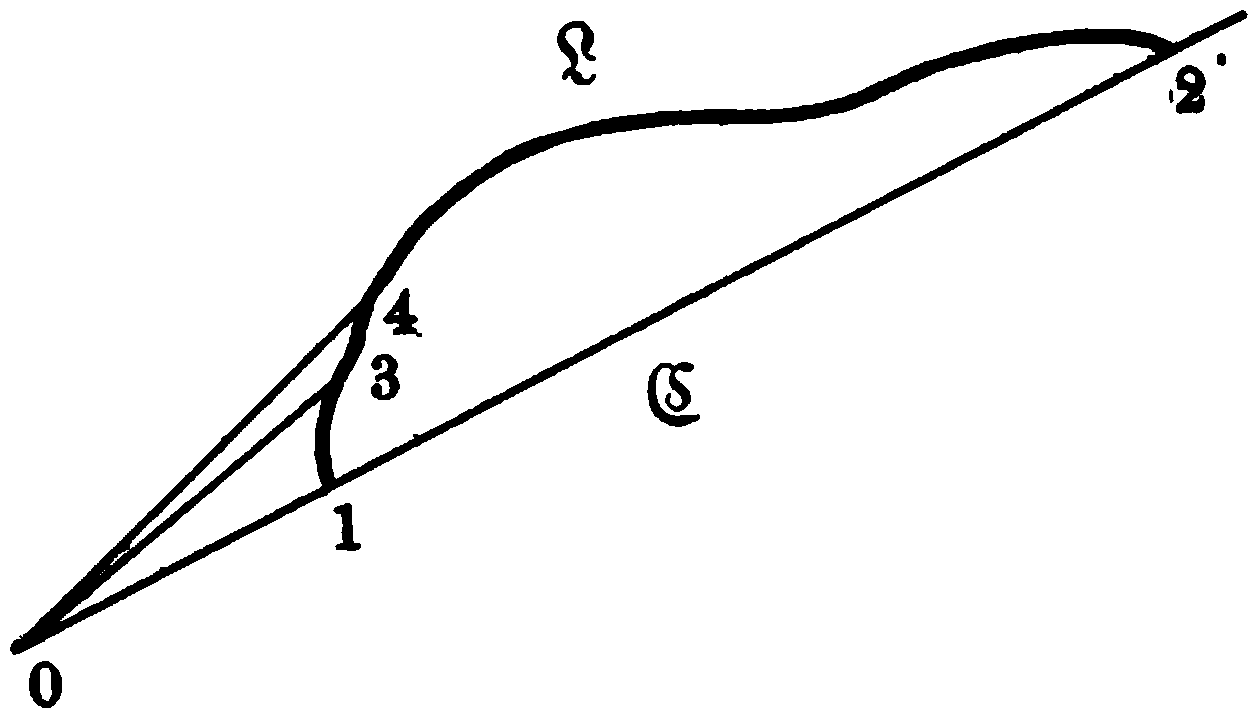
\includegraphics[width=\linewidth,height=30mm,keepaspectratio]{figures/fig15_accepted_derivative.png}\par\vspace{1mm}
\end{minipage}
\end{center}
因此，当点4足够接近点3（图~15）且$\alpha$是一个足够小的给定值时，可以通过该场的一条极值曲线将点0和点4连接起来，使得沿这条曲线形成的积分$\overline{K}_{04}$具有值$\omega_3+\alpha$。特别地，设

\[
\alpha=K_{34},
\]
其中该积分是沿曲线 $\Omega$ 形成的；此时表达式（13）的所有自变量，因而所得到的 $a$ 和 $b$ 的值，都是 $\tau$ 的函数，具有 \S~17 中以 $\varphi(\tau)$ 表示的那类性质。对于两条极值曲线 03 和 04，存在如下关系

\[
\overline{K}_{04}=\overline{K}_{03}+K_{34},
\]
由此可得

\[
\overline{K}_{03}+K_{32}=\overline{K}_{04}+K_{42}.
\]
因此，让点 3 移至一个相邻位置，并在该位置以所定义的极值曲线 03 将它同点 0 连接，则量 $\overline{K}_{03}+K_{32}$ 保持不变。若能以这种方式让点 3 遍历整个弧 $\Omega$

% src-pdfpage=0155
% src-break=0155
，并且若 $\mathfrak{C}$ 是所构造的极值曲线 03 的初始位置和终止位置，我们就说魏尔斯特拉斯构造可行。属于极值曲线 03 的量 $a,b$，于是在从 $\tau_1$ 到 $\tau_2$ 的整个区间内都是 $\tau$ 的函数，并具有 \S~17 中各量 $\varphi(\tau)$ 的性质；它们的初值和终值为 $a_0,b_0$，而常量 $\overline{K}_{03}+K_{32}$ 在 $\tau=\tau_1$ 和 $\tau=\tau_2$ 时分别取值

\[
\overline{K}_{01}+K_{12},
\quad
\overline{K}_{02}=\overline{K}_{01}+\overline{K}_{12}
\]
；这两个值根据（12）相等。在某些特殊问题中，常可判明魏尔斯特拉斯构造是可行的；我们将在 \S~38 中导出其可实施性的一般条件。

现在为了更接近积分 $J$ 的极值问题，我们假设魏尔斯特拉斯的构造是可能的，形成量

\[
W=\overline{J}_{03}+J_{32},
\]
其中第一个积分沿所构造的极值曲线 03 取，第二个积分沿曲线 $\Omega$ 取。这个量是 \S~17 意义下的函数 $\varphi(\tau)$；又因为极值曲线 03 最终过渡到位置 $\mathfrak{C}$，所以有

\[
W\bigg|_{\tau_1}=\overline{J}_{01}+J_{12},
\quad
W\bigg|_{\tau_2}=\overline{J}_{01}+\overline{J}_{12}=\overline{J}_{02}.
\]
因此，若能证明量 $dW$ 的符号为定值，则差 $\overline{J}_{12}-J_{12}$ 亦具有相同的符号。但量 $dW$ 可根据 \S~35 的公式明确地表示出来；因为 $\overline{K}_{03}+K_{32}$ 为常数，所以

\[
\frac{d(\overline{K}_{03}+K_{32})}{d\tau}=0
\]
成立，故有

\[
\frac{dW}{d\tau}=\frac{d\overline{J}_{03}}{d\tau}+\lambda\frac{d\overline{K}_{03}}{d\tau}
+\frac{dJ_{32}}{d\tau}+\lambda\frac{dK_{32}}{d\tau},
\]
其中 $\lambda$ 是极值曲线 03 的等周常数。利用公式（11）和显然正确的方程

\[
\frac{dJ_{32}}{d\tau}=-F\left(x,y,\frac{dx}{d\tau},\frac{dy}{d\tau}\right),
\quad
\frac{dK_{32}}{d\tau}=-G\left(x,y,\frac{dx}{d\tau},\frac{dy}{d\tau}\right)
\]
由此得出

% src-pdfpage=0156
% src-break=0156
\begin{equation}\tag{14}
\frac{dW}{d\tau}=H_{x'}(x,y,\xi_t,\eta_t)\frac{dx}{d\tau}
+H_{y'}(x,y,\xi_t,\eta_t)\frac{dy}{d\tau}
-H\left(x,y,\frac{dx}{d\tau},\frac{dy}{d\tau}\right).
\end{equation}
这个表达式与先前通过

\[
\frac{1}{d\tau}\mathfrak{E}(x,y,x',y',Dx,Dy)=
\mathfrak{E}\left(x,y,x',y',\frac{dx}{d\tau},\frac{dy}{d\tau}\right)
\]
所表示的表达式完全相同，只是其中的 $F$ 已由 $H$ 代替；因此可以运用上文（\S~21）推导的 $\mathfrak{E}$ 的性质，特别可以区分正常消失与异常消失。若 $\mathfrak{E}$ 始终具有恒定符号，并且在所考察的每条曲线 $\Omega$ 上都不恒等于零，那么弧 12 确实给出所求的积分 $J$ 的极值。

如果 $\mathfrak{E}$ 沿曲线 $\Omega$ 的有限部分处处正常消失，那么沿该部分

\[
\frac{dx}{d\tau}=m\xi_t,
\quad
\frac{dy}{d\tau}=m\eta_t,
\quad
m>0;
\]
但是这些方程也

\[
x=\xi,
\quad
 y=\eta
\]
按照 $\tau$ 可以进行微分，因此得出

\begin{equation}\tag{15}
\begin{aligned}
\xi_t\frac{dt}{d\tau}+\xi_a\frac{da}{d\tau}+\xi_b\frac{db}{d\tau}&=m\xi_t,\\
\eta_t\frac{dt}{d\tau}+\eta_a\frac{da}{d\tau}+\eta_b\frac{db}{d\tau}&=m\eta_t.
\end{aligned}
\end{equation}
此外显然

\[
\frac{d\omega}{d\tau}=\omega_t\frac{dt}{d\tau}+\omega_a\frac{da}{d\tau}+\omega_b\frac{db}{d\tau},
\quad
\omega_t=G(\xi,\eta,\xi_t,\eta_t);
\]
既然 $\overline{K}_{03}+K_{32}$ 与 $\tau$ 无关，因此得出

\[
\frac{d\overline{K}_{03}}{d\tau}=-\frac{dK_{32}}{d\tau}=\frac{d\omega}{d\tau}=G\left(\xi,\eta,\frac{dx}{d\tau},\frac{dy}{d\tau}\right)
=mG(\xi,\eta,\xi_t,\eta_t)=m\omega_t,
\]
或者

\[
\frac{d\omega}{d\tau}=\omega_t\frac{dt}{d\tau}+\omega_a\frac{da}{d\tau}+\omega_b\frac{db}{d\tau}=m\omega_t.
\]
但是，可以把这个方程同（15）所列各方程一起，关于下列各量

% src-pdfpage=0157
% src-break=0157
\[
\frac{da}{d\tau},
\quad
\frac{db}{d\tau},
\quad
\frac{dt}{d\tau}-m
\]
看成齐次线性方程组；由于其系数行列式与 $\Delta$ 恒等，因而不为零，所以这三个方程只有在下列条件成立时才能同时成立：

\[
\frac{da}{d\tau}=\frac{db}{d\tau}=0.
\]
由此可以看出，由于$a$和$b$通过魏尔斯特拉斯的构造作为$\varphi(\tau)$函数在\S~17的意义下被确定，如果3和4是所考虑的弧上的任意两点，就会得出

\[
a\bigg|_4^3=b\bigg|_4^3=0;
\]
因此，该弧是场内一条极值曲线的一部分。若 $\mathfrak{E}$ 沿整条曲线 $\Omega$ 正常消失，则由于 $a_0,b_0$ 是 $a,b$ 的终值，$\Omega$ 必须与 $\mathfrak{C}$ 重合。若非如此，并且 $\mathfrak{E}$ 的异常消失与符号改变已被排除——或一般地排除，或通过限制所比较的曲线 $\Omega$ 来排除——则差

\[
W\bigg|_{\tau_1}^{\tau_2}=\int_{\tau_1}^{\tau_2}\mathfrak{E}\,d\tau=\overline{J}_{12}-J_{12}
\]
不等于零，并且与 $\mathfrak{E}$ 具有相同的符号，从而保证了极值的存在。

总之，至此已证明有三个条件足以保证极值的出现：1）场的存在，即雅可比条件；2）魏尔斯特拉斯符号条件，即量 $\mathfrak{E}$ 在上述意义下具有固定符号；3）能够在场内实行魏尔斯特拉斯构造。若这些条件满足，则极值曲线 $\mathfrak{C}$ 使积分 $J_{12}$ 取得极值；比较曲线为场内的曲线 12 或 $\Omega$，并使 $K_{12}$ 取指定值。视 $\mathfrak{E}$ 的符号是无条件得到保证，还是仅在 $\Omega$ 位于曲线 $\mathfrak{C}$ 的较小邻域内时得到保证，该极值分别为强极值或弱极值。

这里，极值一般不是由始于点 0 的弧给出，而是由

% src-pdfpage=0158
% src-break=0158
弧 12 给出；其起点 1 可以任意接近位置 0。

此外，在 \S~21 的一般讨论中把函数 $F$ 用 $H$ 代替，便可看出：只要下列量具有固定符号，这里考察的量 $\mathfrak{E}$ 也具有固定符号：

\[
H_1=\frac{1}{y'^2}H_{x'x'}=\frac{1}{x'^2}H_{y'y'}=
\frac{1}{x'^2}(F_{y'y'}+\lambda G_{y'y'})
\]
或者，若 $x'$ 不为零，上述结论也可由乘积 $(f_{pp}+\lambda g_{pp})dx$ 具有固定符号推出。因此，只要在 \S~17 的勒让德条件中用 $F+\lambda G$ 代替 $F$，就可以用该条件替代魏尔斯特拉斯符号条件。

若条件 1）与 2）满足，则在让积分 $J,K$ 互换原有作用后所得的问题中，这两个条件仍然满足。对于条件 1），这直接由上述说明得出：某些极值曲线形成一个场的性质在这种互换下保持不变。对于条件 2），类似的结论来自 $H$ 和 $\mathfrak{E}$ 分别由

\[
G+\frac{1}{\lambda}F,
\quad
\frac{1}{\lambda}\mathfrak{E}
\]
替换；由于 $\lambda$ 不为零，若 $\mathfrak{E}$ 具有固定符号，后一个量显然也具有固定符号，不过其符号不必与 $\mathfrak{E}$ 的符号相同。因此，新问题中的极值与旧问题中的极值具有相同或相反的性质，取决于 $\lambda$ 为正还是为负。由此证明了迈尔所提出的互反定律的最简单情形。

% machine-unit: Kneser_LVR_DE_p0158low_p0177top §§37-39
% visible source begins below §37 on source pdfpage 0158; p0177 §40 heading/body excluded from this slice.
% src-pdfpage=0158
% src-break=0158
\begin{center}
{\large \S~37.}
\end{center}
\noindent\textbf{例。问题九（\S~34）。} 极值曲线是半径为 $\pm\lambda$ 的圆；经过某一点 0，例如坐标原点的那些极值曲线可以用以下方式表示。设 $a,b$ 是圆心 $m$ 的坐标，半径为 $r$ （图~16）；那么可以设

\begin{equation}\tag{16}
 x=a+r\cos\theta,\quad y=b+r\sin\theta,\quad r^2=a^2+b^2
\end{equation}
并且 $\theta$ 是半径从与 $+x$ 轴平行的位置 $mx$ 出发，按正向旋转方向所描述的角度，以使其端点到达所考虑的圆上的点 4；正向旋转方向如通常所定义，即绕 $90^\circ$ 旋转后

% src-pdfpage=0159
% src-break=0159
将 $+x$ 轴转换为 $+y$ 轴。

\begin{center}
\begin{minipage}{0.48\linewidth}\centering
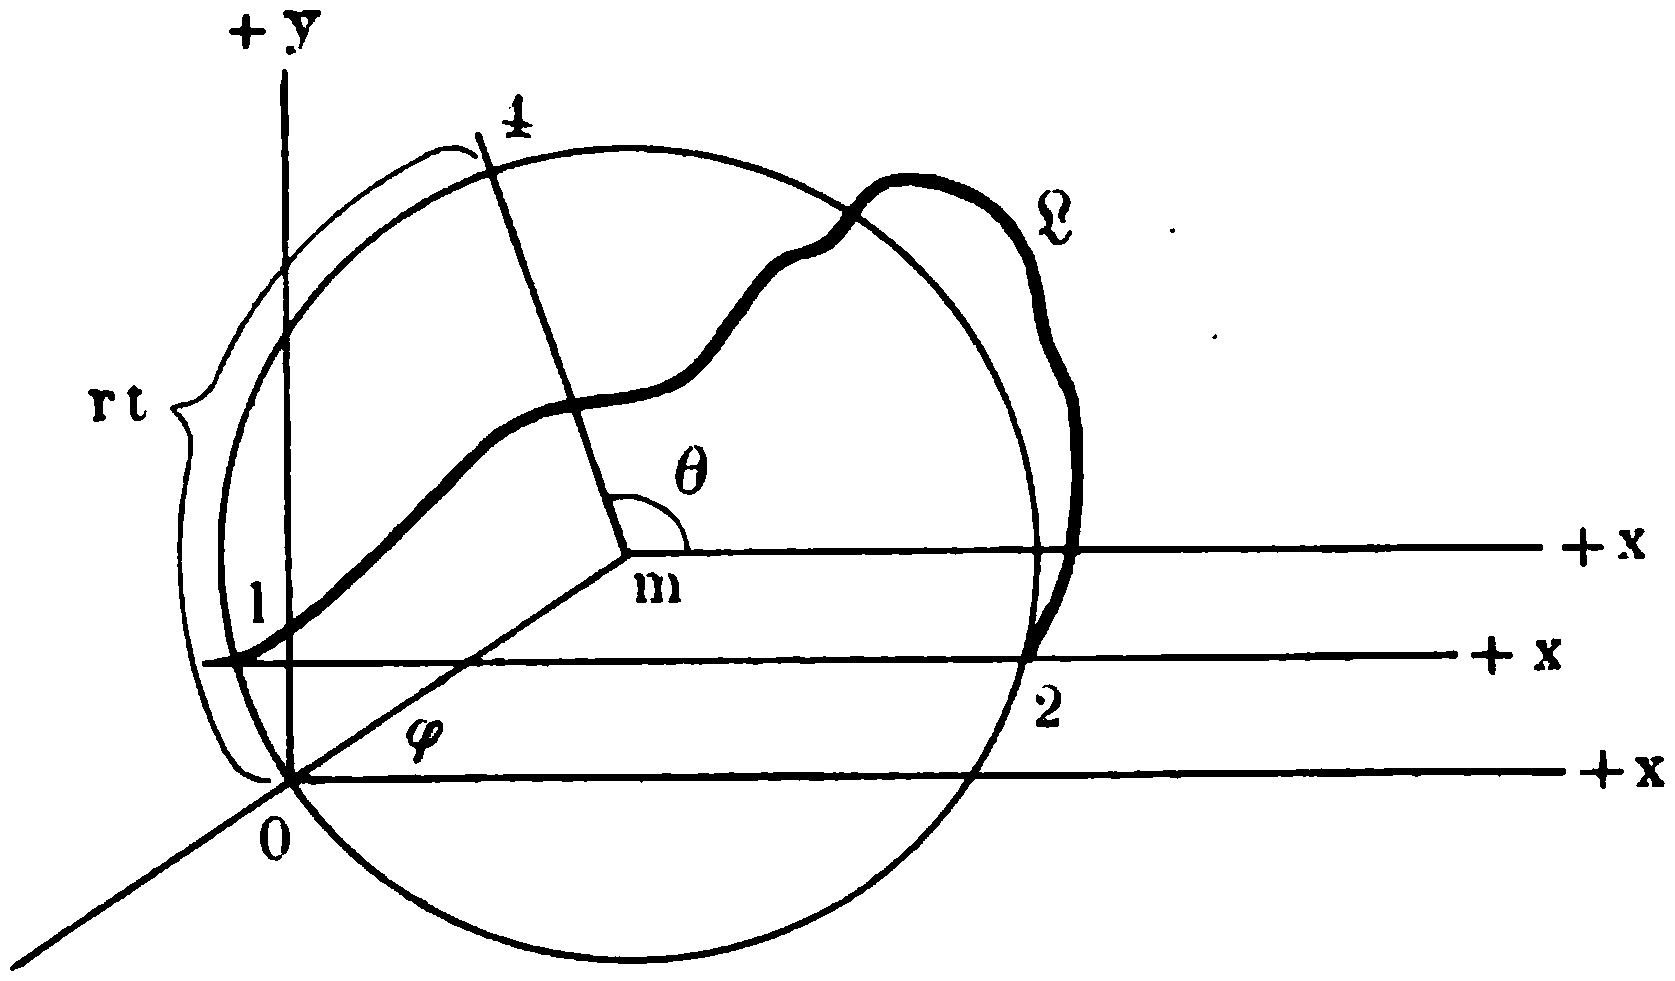
\includegraphics[width=\linewidth,height=36mm,keepaspectratio]{figures/fig16_accepted_derivative.png}\par\vspace{1mm}
\end{minipage}
\end{center}
此外，若 $\varphi$ 是射线 $0m$ 与 $+x$ 轴之间，按正方向测量的夹角，则有

\begin{equation}\tag{17}
 a=r\cos\varphi,\quad b=r\sin\varphi,
\end{equation}
因此半径 $m0$ 的倾角为 $\varphi+\pi$，这是相对于 $mx$ 而言的。因此，设

\[
 t=\pi+\varphi-\theta,\quad \theta=\pi+\varphi-t,
\]
所以 $rt$ 是从点 0 向负方向测量的圆弧 04，根据（16）、（17）式，有

\[
 K_{04}=\omega=t\sqrt{a^2+b^2},\quad
 \xi(t,a,b)=a-a\cos t-b\sin t,
\]
\[
 \eta(t,a,b)=b-b\cos t+a\sin t.
\]
这些函数在处处都是正则的，只要 $r$ 保持在两个任意的正界限之间。此外还有

\[
\Delta=\begin{vmatrix}
1-\cos t&\sin t&\dfrac{at}{r}\\[1.0ex]
-\sin t&1-\cos t&\dfrac{bt}{r}\\[1.0ex]
a\sin t-b\cos t&a\cos t+b\sin t&r
\end{vmatrix},
\]
并且当把 $a$ 和 $b$ 表示为另一些变量 $\alpha,\beta$ 的函数时，

\begin{equation}\tag{18}
\frac{\partial(\xi,\eta,\omega)}{\partial(t,\alpha,\beta)}=
\frac{\partial(\xi,\eta,\omega)}{\partial(t,a,b)}\cdot
\frac{\partial(t,a,b)}{\partial(t,\alpha,\beta)}
=\Delta\frac{\partial(a,b)}{\partial(\alpha,\beta)};
\end{equation}
特别地，$\alpha,\beta$ 是点 $m$ 在新坐标系中的直角坐标，那么 $\Delta$ 旁边的因子具有值

% src-pdfpage=0160
% src-break=0160
$\pm1$。若特别有 $b=0$，则 $a^2=r^2$，并有

\[
\begin{aligned}
\Delta&=r\begin{vmatrix}
1-\cos t&\sin t&t\\
-\sin t&1-\cos t&0\\
\sin t&\cos t&1
\end{vmatrix}\\
&=r(2-2\cos t-t\sin t)=4r\sin\frac{t}{2}\left(\sin\frac{t}{2}-\frac{t}{2}\cos\frac{t}{2}\right).
\end{aligned}
\]
而当点 4 沿所考察的圆移动时，$t$ 在区间

\begin{equation}\tag{19}
0\leq t<2\pi,
\end{equation}
因此，除点 0 外，表达式 $\Delta$ 的各因子均不为零。若 $b$ 不为零，就把坐标系 $(a,b)$ 换成新的坐标系 $(\alpha,\beta)$，使其横轴通过 $m$；于是根据公式（18），$\Delta$ 仍不为零。由此证明：所有经过点 0 且在 $\varepsilon,\gamma$ 为正常数时满足不等式

\begin{equation}\tag{20}
\varepsilon^2<a^2+b^2<\gamma^2
\end{equation}
的圆构成 \S~36 意义下的一个场，只要用不等式（19）限制 $t$，即认为每个圆至多遍历一次。

在这种任务中

\[
F=yx',\quad G=\sqrt{x'^2+y'^2},\quad H=yx'+\lambda\sqrt{x'^2+y'^2},
\]
并且平方根为正，因此有

\[
\begin{aligned}
\mathfrak{E}&=\left(y+\frac{\lambda x'}{\sqrt{x'^2+y'^2}}\right)Dx+
\frac{\lambda y'}{\sqrt{x'^2+y'^2}}Dy-
\left(yDx+\lambda\sqrt{Dx^2+Dy^2}\right)\\
&=\lambda\sqrt{Dx^2+Dy^2}\left\{\frac{x'}{\sqrt{x'^2+y'^2}}\frac{Dx}{\sqrt{Dx^2+Dy^2}}+
\frac{y'}{\sqrt{x'^2+y'^2}}\frac{Dy}{\sqrt{Dx^2+Dy^2}}-1\right\};
\end{aligned}
\]
括号内的量（\S~23，问题一）从不为正，且 $\mathfrak{E}$ 仅当下列条件成立时才消失

\[
\frac{x'}{\sqrt{x'^2+y'^2}}=\frac{Dx}{\sqrt{Dx^2+Dy^2}},\quad
\frac{y'}{\sqrt{x'^2+y'^2}}=\frac{Dy}{\sqrt{Dx^2+Dy^2}},
\]
也就是说，只以正常方式消失。此外，$t$ 增大方向相对于向外半径的取向，正如
% END PHYSICALLY EMBEDDED BODY INH04 1/5
% BEGIN PHYSICALLY EMBEDDED BODY INH04 2/5: inherited/INH04_pdf151_200_producer_r2/work/zh_161_170.tex
% src-pdfpage=0161
% src-break=0161
$+x$ 轴相对于 $+y$ 轴的取向；所以按 \S~34，$\lambda$ 为负，$\mathfrak{E}$ 为正，所求极值为极大值。

现在用一段圆弧连接点 1 与点 2；点 0 在圆上，但位于这段弧外。过点 0 作横轴平行于直线 12，并规定 $y$ 轴的方向，使直线 12 上 $y$ 为正。于是，上述定义的 $t$ 增大方向沿弧 $\mathfrak{C}$ 从点 1 指向点 2，而积分

\[
\overline{J}_{12}=\int_1^2 yx'\,dt
\]
是 $\mathfrak{C}$ 与直线段 12 之间的正面积，加上由后者纵坐标所覆盖的矩形面积。再者，设 $\Omega$ 是任意一条连接 1 和 2 的曲线，具有与 \S~17 中相同的连续性性质，并且与 $\mathfrak{C}$ 具有相同的长度，且不进入以 0 为中心、半径为 $2\varepsilon$ 的圆内，这通过适当选择该点总是可以实现的。那么，所有通过 0 和曲线 $\Omega$ 上某一点 3 的圆，其半径都大于 $\varepsilon$。如果限制这些圆的半径不超过某一界限 $\gamma$，则它们都属于场 (20)。

现在，当点 3 遍历弧 $\Omega$ 时，在每个位置用一段圆弧把它同点 0 连接起来，该圆弧的长度为

\[
\overline{K}_{01}+K_{13}=\operatorname{arc}01+\operatorname{arc}13,
\]
其中第一段弧在圆 012 上量取，第二段弧在曲线 $\Omega$ 上量取。这个量大于直线距离 03，所以所求弧的半径有限；又因该半径显然随点 3 连续变化，故有一个有限上界 $\gamma$。在关于直线 03 对称、具有所需性质的两个圆弧中，我们始终选取从初始位置 $\mathfrak{C}$ 连续生成的那个；由于半径保持有限，$\mathfrak{C}$ 也是弧 03 的终止位置，从而已充分证明魏尔斯特拉斯构造在场（20）内可行。因此，\S~36 的一般理论给出

\[
\overline{J}_{12}>J_{12},
\]
即由圆弧 $\mathfrak{C}$ 和直线段 12 所围成的

% src-pdfpage=0162
% src-break=0162
圆弓形面积大于由曲线 $\Omega$ 所界定的相应面积。显然，这里证明的结论还强于极大性质本身。

\begin{center}
{\large \S~38.}
\end{center}
若对曲线 $\Omega$ 施加一种在许多问题中自然出现的限制，魏尔斯特拉斯构造便可实行；该限制要求：在曲线 $\Omega$ 与 $\mathfrak{C}$ 的相邻点处，从点 0 起沿两条曲线形成的积分 $K$ 也只相差很小。为更精确地表述这一规定，设点 6 遍历任一条从点 0 出发的曲线，$K_{06}$ 是沿该曲线得到的积分，而 $z$ 是第三个直角空间坐标。于是一般地令

\[
x=x_6,\quad y=y_6,\quad z=K_{06},
\]
这样，点 $(x,y,z)$ 描出一条也从点 0 出发的空间曲线；把以这种方式对应于任意原平面点 $1,\ldots,6$ 的空间点记为 $1^0,\ldots,6^0$。于是，场的每一条极值曲线都对应一条曲线

\[
x=\xi(t,a,b),\quad y=\eta(t,a,b),\quad z=\omega(t,a,b);
\]
对于 $a=a_0,b=b_0$，可以得到一条与曲线 $\mathfrak{C}$ 相应的空间曲线 $\mathfrak{C}^0$。由极值曲线弧 01 和曲线 $\Omega$ 组成的线，对应一条空间曲线，该曲线直到点 $1^0$，其坐标

\[
x=x_1,\quad y=y_1,\quad z=\overline{K}_{01}=\omega(t_1,a_0,b_0)
\]
与 $\mathfrak{C}^0$ 重合，然后又从此处分开；点 $3^0$ 的坐标

\begin{equation}\tag{21}
x=x_3,\quad y=y_3,\quad z=\overline{K}_{01}+K_{13}.
\end{equation}
新规定是：只把曲线 $\Omega$ 与 $\mathfrak{C}$ 比较积分 $J$ 的值，并且只允许其相应空间曲线 $\Omega^0$ 属于曲线 $\mathfrak{C}^0$ 的某一邻域（\S~17）。

在后一条空间曲线上，弧 12 的点 5 对应一个点 $5^0$，对它有

\[
x=x_5,\quad y=y_5,\quad z=\overline{K}_{05}=\omega(t_5,a_0,b_0)=z_5;
\]
然后这些方程可以

% src-pdfpage=0163
% src-break=0163
\begin{equation}\tag{22}
\begin{aligned}
x-x_5&=\xi(t,a,b)-x_5=[t-t_5,a-a_0,b-b_0]_1,\\
y-y_5&=\eta(t,a,b)-y_5=[t-t_5,a-a_0,b-b_0]_1,\\
z-z_5&=\omega(t,a,b)-z_5=[t-t_5,a-a_0,b-b_0]_1,
\end{aligned}
\end{equation}
其中右边线性项的行列式为 $\Delta(t_5,a_0,b_0)$；把 $t-t_5,a-a_0,b-b_0$ 分别代入如下形式的某些确定级数，便可满足这些方程：

\[
[x-x_5,\ y-y_5,\ z-z_5]_1
\]
这些表达式把 $t,a,b$ 定义为 $x,y,z$ 的函数；这些函数在每一点 $5^0$ 都是正则的。因此，当曲线 $\mathfrak{C}$ 不与自身相交，即不同的 $t_5$ 值对应不同的点 $5^0$ 时，这些函数在包含弧 $1^02^0$ 的某一区域 $\mathfrak{G}^0$ 内正则且唯一确定，从而该区域恰好被与上述表达式所定义的 $a,b$ 对应的极值曲线单重填满。如果所考虑的点落在曲线 $\mathfrak{C}^0$ 本身上，那么 $a$ 和 $b$ 就变为 $a_0$ 和 $b_0$。区域 $\mathfrak{G}^0$ 可以想象为一个球体在其球心沿弧 $1^02^0$ 移动时所扫过的空间。

现在，如果曲线 $\Omega^0$ 完全位于区域 $\mathfrak{G}^0$ 的内部，那么每个点 $3^0$ 都位于该场中定义的某条特定极值曲线之上，这时人们就有方程

\[
x_3=\xi(t_3,a,b),\quad y_3=\eta(t_3,a,b),\quad z_3=\omega(t_3,a,b).
\]
由此可得，根据第三式（21）

\[
\omega(t_3,a,b)=\overline{K}_{03}=\overline{K}_{01}+K_{13},
\]
因此

\[
\overline{K}_{03}+K_{32}=\overline{K}_{01}+K_{13}+K_{32}=\overline{K}_{01}+K_{12}=\overline{K}_{02};
\]
所构造的曲线 $03^0$ 在 $xy$ 平面上的投影正好就是魏尔斯特拉斯构造中所寻求的极值曲线 03，并且根据与方程 (22) 相关联的注释，它过渡到 $\mathfrak{C}$当点 $3^0$ 移动到位置 $1^0$ 和 $2^0$ 之一时。在新引入的对曲线 $\Omega$ 的限制下，魏尔斯特拉斯的构造总是可能的，并且在 \S~36 中所给出的极值的充分条件之一将不复存在。

\noindent\textbf{例。问题十一。} 把一根长度与端点给定的均匀重绳置于竖直

% src-pdfpage=0164
% src-break=0164
平面内，使其重心尽可能低（平衡形状，悬链线）。

如果 $+y$ 轴是重力方向，$l$ 是绳子 01 的长度，单位长度的质量为 1，那么质心的纵坐标

\[
\frac{1}{l}\int_0^1 y\sqrt{x'^2+y'^2}\,dt,
\]
因此，积分

\[
J=\int_0^1 y\sqrt{x'^2+y'^2}\,dt
\]
应在弧积分

\[
K=\int_0^1 \sqrt{x'^2+y'^2}\,dt,
\]
取给定值的条件下达到极大；并且积分

\[
J+\lambda K=\int (y+\lambda)\sqrt{x'^2+y'^2}\,dt
\]
的第一变分应设为零。对于极值曲线，由此可得（\S~9，问题 II）方程

\[
y+\lambda=\frac{a}{2}\left\{e^{\frac{x-b}{a}}+e^{-\frac{x-b}{a}}\right\}=a\Cof\frac{x-b}{a}.
\]
右边对于 $x=\pm\infty$ 具有大小 $a$ 的符号，因此曲线对于 $a<0$ 是向下凸的。那么 $y+\lambda$ 始终为负，而大小

\[
\mathfrak{E}=(y+\lambda)\sqrt{Dx^2+Dy^2}\left\{\frac{x'Dx+y'Dy}{\sqrt{x'^2+y'^2}\sqrt{Dx^2+Dy^2}}-1\right\}
\]
为正；并且 $=0$ 当且仅当值组 $(x',y')$ 和 $(Dx,Dy)$ 表示同一方向。因此，魏尔斯特拉斯的强极大符号条件得到满足。

进一步的计算借助于以下易于证明的公式而简化

\begin{equation}\tag{23}
\begin{aligned}
\Cof(u+v)&=\Cof u\Cof v+\Sin u\Sin v,\\
\Sin(u+v)&=\Sin u\Cof v+\Sin v\Cof u.
\end{aligned}
\end{equation}
通过固定点0的极值曲线的常数满足关系

\[
y_0+\lambda=a\Cof\frac{x_0-b}{a},
\]
% src-pdfpage=0165
% src-break=0165
因此，这族曲线的一般方程可以写成

\[
y-y_0=a\left\{\Cof\frac{x-b}{a}-\Cof\frac{x_0-b}{a}\right\}.
\]
这个方程的右边是正则的，只要 $a$ 不等于零，人们就可以设为

\[
x=\xi(t,a,b)=t,\quad y=\eta(t,a,b)=y_0+a\left\{\Cof\frac{t-b}{a}-\Cof\frac{t_0-b}{a}\right\}.
\]
既然如此

\[
\xi_t=1,\quad \xi_a=\xi_b=0,
\]
因此

\[
\Delta(t,a,b)=\frac{\partial(\xi,\eta,\omega)}{\partial(t,a,b)}=\frac{\partial(\eta,\omega)}{\partial(a,b)}.
\]
进一步，$\omega$是从点0开始测量的弧长，即

\[
\omega=\int_0^t\sqrt{1+y'^2}\,dt=\int_0^t\sqrt{1+\Sin^2\frac{t-b}{a}}\,dt
=\int_0^t \Cof\frac{t-b}{a}\,dt,
\]
\[
=a\left\{\Sin\frac{t-b}{a}-\Sin\frac{t_0-b}{a}\right\};
\]
因此，当

\[
\frac{t-b}{a}=u,
\quad
\frac{t_0-b}{a}=u_0
\]
作上述设定时，根据双曲函数的微分公式（\S~23）

\[
-\Delta=\begin{vmatrix}
\Cof u-\Cof u_0-(u\Sin u-u_0\Sin u_0)&\Sin u-\Sin u_0\\
\Sin u-\Sin u_0-(u\Cof u-u_0\Cof u_0)&\Cof u-\Cof u_0
\end{vmatrix};
\]
进一步求导并利用方程(23)，可得

\[
\begin{aligned}
-\frac{d\Delta}{du}&=\begin{vmatrix}
-u\Cof u&\Sin u-\Sin u_0\\
-u\Sin u&\Cof u-\Cof u_0
\end{vmatrix}
+\begin{vmatrix}
\Cof u-u\Sin u-\Cof u_0+u_0\Sin u_0&\Cof u\\
\Sin u-u\Cof u-\Sin u_0+u_0\Cof u_0&\Sin u
\end{vmatrix}\\
&=(u-u_0)\Cof(u-u_0)-\Sin(u-u_0).
\end{aligned}
\]
由此得出

\[
-\frac{d^2\Delta}{du^2}=(u-u_0)\Sin(u-u_0);
\]
由于量 $u-u_0$ 和 $\Sin(u-u_0)$ 具有相同的符号，因此总是

% src-pdfpage=0166
% src-break=0166
\[
\frac{d^2\Delta}{du^2}\leq0;
\]
由于进一步地，量 $\Delta$ 和 $d\Delta:du$ 对于 $u=u_0$ 消失，因此后者始终具有 $u_0-u$ 的符号，而前者只要 $u\gtrless u_0$ 就为负。现在从点 0 出发，沿着增大的 $x$ 方向沿悬链线前进，那么

\[
u-u_0=\frac{x-x_0}{a}
\]
与 $a$ 相同地为负，$\Delta$ 也因此为负；因此，对于任意长的一段向下凸的悬链线，强极大值的充分条件在上述对曲线 $\Omega$ 的限制下均得到满足。根据 \S~36 中所作的说明，极大值首先对于每个起点距离 0 非常近的弧 12 成立；由于点 0 的位置不受任何限制，因此弧 12 可以被视为曲线的任意一部分。

所引入的对曲线 $\Omega$ 的限制在这里是自然的，因为每当一根线稍微移动时，由从点 0 开始测量的特定线长所定义的单个物质点，就被认为只是略微移动了。曲线 $\Omega$ 和 $\mathfrak{C}$ 然后被唯一地相互关联，使得对应的点之间的距离很小，并且给出积分 $K$ 的相同值。

\begin{center}
{\large \S~39.}
\end{center}
若作如下假定，则前几节的一般推演只需稍加修改仍然成立：所考察的极值曲线族

\begin{equation}\tag{24}
x=\xi(t,a,b),\quad y=\eta(t,a,b),
\end{equation}
（曲线 $\mathfrak{C}$ 属于该族）不经过固定点 0，而是全都横截一条固定曲线 $\mathfrak{C}_0$；于是可得到判据，使曲线 $\mathfrak{C}$ 的一段在所有把一个固定点同曲线 $\mathfrak{C}_0$ 连接起来、并使积分 $K$ 取指定值的曲线中给出积分的极值。

设

\[
\Gamma(x,y)=0
\]
% src-pdfpage=0167
% src-break=0167
为曲线 $\mathfrak{C}_0$ 的方程；该曲线在可变点 0 处以非零角横截 $\mathfrak{C}$ 以及族（24）中充分接近前述极值曲线的各曲线，并且在该点正则。于是有方程

\begin{equation}\tag{25}
\Gamma[\xi(t_0,a,b),\eta(t_0,a,b)]=0,
\end{equation}
该方程可以对 $t_0$ 解出，因为在所考察的点 0 处有不等式

\[
\Gamma_x\xi_t+\Gamma_y\eta_t\neq0
\]
成立。因此，当$t_{00}$是参数，它属于曲线$\mathfrak{C}$与$\mathfrak{C}_0$的交点时，

\[
t_0-t_{00}=[a-a_0,b-b_0]_1.
\]
此外，由于族（24）的极值曲线与曲线 $\mathfrak{C}_0$ 横截相交，因此在假设

\[
\left.\Gamma_xDx+\Gamma_yDy\right|^0=0
\]
之下，恒可得方程

\[
\left.H_{x'}Dx+H_{y'}Dy\right|^0=0;
\]
由此可得

\begin{equation}\tag{26}
\left.\Delta=H_{x'}\Gamma_y-H_{y'}\Gamma_x\right|^0=0,
\end{equation}
其中各自变量

\begin{equation}\tag{27}
x=\xi,\quad y=\eta,\quad x'=\xi_t,\quad y'=\eta_t
\end{equation}
应予以采用。然后对公式（25）对$a$和$b$求导，可得

\[
\left.\Gamma_x\left(\xi_t\frac{\partial t_0}{\partial a}+\xi_a\right)+\Gamma_y\left(\eta_t\frac{\partial t_0}{\partial a}+\eta_a\right)\right|^0=0,
\]
\[
\left.\Gamma_x\left(\xi_t\frac{\partial t_0}{\partial b}+\xi_b\right)+\Gamma_y\left(\eta_t\frac{\partial t_0}{\partial b}+\eta_b\right)\right|^0=0.
\]
在这些方程中，根据（26），可以把量 $\Gamma_x$ 和 $\Gamma_y$ 分别换成 $H_{x'}$ 和 $H_{y'}$；于是它们就与公式（9）完全相同。因此，沿该族中变量点 3 所在的任一条极值曲线取积分

\[
\overline{J}_{03}=\int_0^3 F\,dt=\int_{t_0}^{t}F(\xi,\eta,\xi_t,\eta_t)\,dt,\quad
\overline{K}_{03}=\int_{t_0}^{t}G(\xi,\ldots,\eta_t)\,dt,
\]
首先，与 $t_0,a,b$ 之间的关系无关的方程（7）在这里仍然成立，并由它得到

% src-pdfpage=0168
% src-break=0168
正如在 \S~35 中根据公式 (9) 推导出方程 (10)、(11)。

现在仍如上令

\[
\overline{K}_{03}=\omega(t,a,b)
\]
，并假设行列式

\[
\Delta=\frac{\partial(\xi,\eta,\omega)}{\partial(t,a,b)}
\]
沿着属于曲线 $\mathfrak{C}$ 的弧 02，除了点 0 以外，不消失；那么对于所有从曲线 $\mathfrak{C}_0$ 开始的极值曲线族的弧，这些弧与 02 足够接近时，同样成立；所有使得 $\Delta$ 不为零的弧的全体，称为弧 02 的场。在曲线 $\mathfrak{C}_0$ 本身，$\Delta$ 处处消失，如公式 (7)、(9) 易得。然后，如在 \S~35 所进行的讨论现在也表明，弧 02 的某一邻域，一般来说被场的极值曲线无限多次覆盖。在该邻域内，取属于曲线 $\mathfrak{C}_0$ 的点 1，用一条线 $\Omega$ 与点 2 连接，对于这条线，方程

\begin{equation}\tag{28}
K_{12}=\overline{K}_{02}
\end{equation}
成立，其中等式右端的积分沿曲线 $\mathfrak{C}$ 计算，而不带横线的积分仍始终指曲线 $\Omega$。让点 3 沿后者移动；于是，与魏尔斯特拉斯构造类似的构造，是作一条随点 3 变化的场内极值曲线，使量 $\overline{K}_{03}+K_{32}$ 保持常数，并在点 3 与点 2 重合时过渡为曲线 $\mathfrak{C}$。该量的初值和终值显然就是方程（28）的两边。

在\S~38中给出的关于魏尔斯特拉斯构造可能性的证明，不能直接应用于当前的问题，因为$\Delta$在曲线$\mathfrak{C}_0$上，如前所述，消失。这一情况对\S~36的论证没有影响，根据该论证，$\mathfrak{E}$只能沿着场的极值曲线处处以正常方式消失；由于现在量$\overline{K}_{03}+K_{32}$与$\tau$无关，而且如已证明，\S~35中的方程(7)、(10)、(11)现在也成立，因此得出如在\S~36中的结论：

% src-pdfpage=0169
% src-break=0169
\[
\frac{dW}{d\tau}=\frac{d(\overline{J}_{03}+J_{32})}{d\tau}
=H_x\frac{dx}{d\tau}+H_y\frac{dy}{d\tau}-H\left(x,y,\frac{dx}{d\tau},\frac{dy}{d\tau}\right)
=\mathfrak{E}\left(x,y,x',y',\frac{dx}{d\tau},\frac{dy}{d\tau}\right).
\]
大小 $W$ 的初始值和终值与先前的不同；显然现在

\[
\left.W\right|^{\tau_1}=J_{12},\quad \left.W\right|^{\tau_2}=\overline{J}_{02};
\]
差 $\overline{J}_{02}-J_{12}$ 因此具有量 $\mathfrak{E}$ 的符号。

因此，若场的极值曲线横截正则曲线 $\mathfrak{C}_0$ 而不与其相切，则 \S~36 中给出的极值充分条件，对于所有把曲线 $\mathfrak{C}_0$ 与一个固定点连接起来的线 $\Omega$ 之中的极值，具有同样的意义。

\noindent\textbf{例。问题九} 按如下方式具体化。从点 2 向圆周 $\mathfrak{C}_0$ 作任意一条固定曲线 $\mathfrak{F}$；再用第二条给定长度的曲线把点 2 同一个圆 $\mathfrak{C}_0$ 连接起来，使它与该圆及曲线 $\mathfrak{F}$ 所围成的面积尽可能大。

\begin{center}
\begin{minipage}{0.45\linewidth}\centering
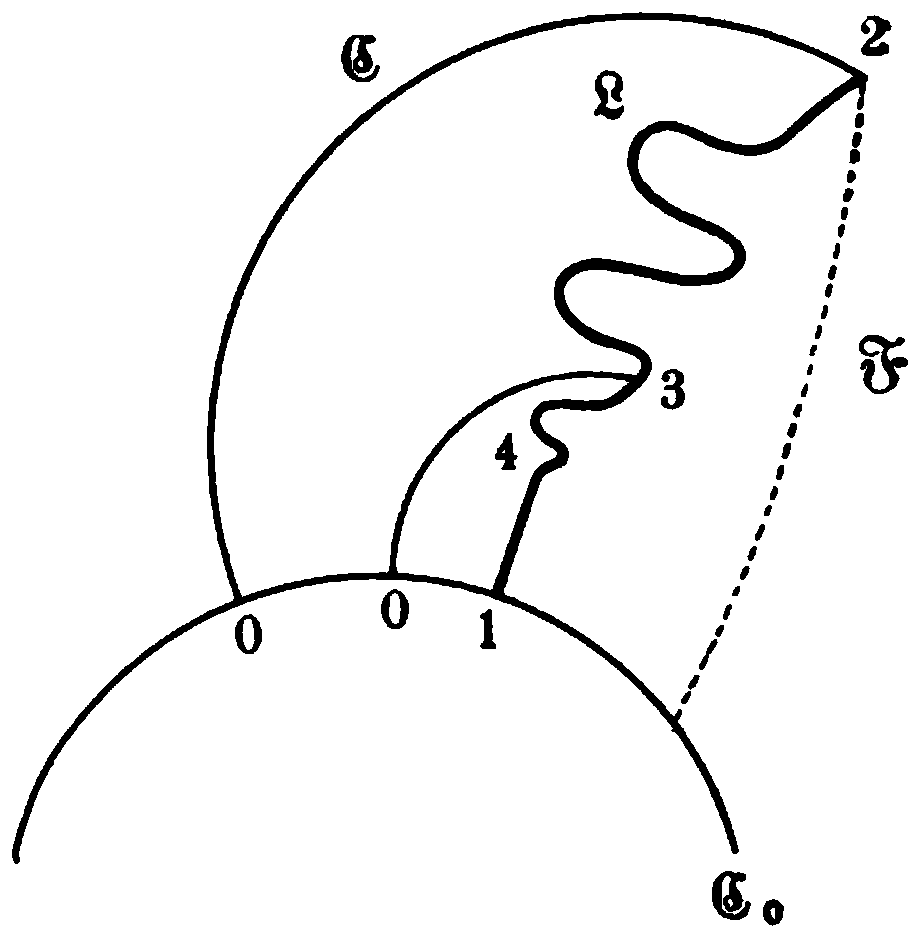
\includegraphics[width=\linewidth,height=42mm,keepaspectratio]{figures/fig17_accepted_derivative.png}\par\vspace{1mm}
\end{minipage}
\end{center}
极值曲线是圆（图~17）；按 \S~34，当它们与圆 $\mathfrak{C}_0$ 垂直相交时，便横截该圆。每个点 3 都能由一条给定长度、正交于圆 $\mathfrak{C}_0$ 的圆弧 03 同该圆连接，只要这个长度大于该点同 $\mathfrak{C}_0$ 之间的最短直线距离；所以魏尔斯特拉斯构造总能沿任一规定长度的弧 $\Omega$ 或 12 进行，使弧 03 等于沿曲线 $\Omega$ 量得的弧 13。还可选择圆弧 03，使一个绕圆 $\mathfrak{C}_0$ 按指定方向 $\mathfrak{R}$ 运动的点，在每个位置 0 都走向弧 03 的凹侧。不过，这一构造只能对

% src-pdfpage=0170
% src-break=0170
弧 $\Omega$ 的弧段 42 实行：若该弧从垂直于圆 $\mathfrak{C}_0$ 的直线段 14 开始、但在点 4 离开直线 14，则当使点 3 与点 4 靠拢时，线段 14 就是弧 03 的极限，因此

\begin{equation}\tag{29}
\left.\overline{J}_{03}+J_{32}\right|^{\tau_4}=J_{12},\quad
\left.\overline{K}_{03}+K_{32}\right|^{\tau_4}=K_{12}
\end{equation}
可以被设定。此外，当点3退回到位置2时，弧03的极限位置是弧$\mathfrak{C}$或02，与$\Omega$进行比较，因此方程

\[
\lim \overline{J}_{03}=\overline{J}_{02}
\]
成立，那么根据（29）

\[
\left.\overline{J}_{03}+J_{32}\right|_{\tau_4}^{\tau_2}=\int_{\tau_4}^{\tau_2}\mathfrak{E}\,d\tau=\overline{J}_{02}-J_{12},
\]
由此，由于 $\mathfrak{E}$ 具有固定的符号，只要满足雅可比条件，极值就成立。

为了确定这种情况在多大范围内成立，我们假设

\[
x_0^2+y_0^2=r^2
\]
是圆 $\mathfrak{C}_0$ 的方程；若 $b$ 是沿方向 $\mathfrak{R}$ 增大的弧长，则

\[
\alpha=x_0+a\frac{dx_0}{db},\quad \beta=y_0+a\frac{dy_0}{db}
\]
是半径为 $|a|$ 的弧 03 的圆心坐标；按 $\mathfrak{R}$ 的上述含义，$a$ 为正。根据 \S~37 所用的表示法，把坐标原点移至点 0 后，圆弧 03 可由下列方程表示：

\[
\begin{aligned}
x-x_0&=(\alpha-x_0)-(\alpha-x_0)\cos t-(\beta-y_0)\sin t,\\
y-y_0&=(\beta-y_0)+(\alpha-x_0)\sin t-(\beta-y_0)\cos t,
\end{aligned}
\]
或者，如果设

\[
\xi(t,a,b)=x_0+a\frac{dx_0}{db}-a\frac{dx_0}{db}\cos t-a\frac{dy_0}{db}\sin t,
\]
\[
\eta(t,a,b)=y_0+a\frac{dy_0}{db}+a\frac{dx_0}{db}\sin t-a\frac{dy_0}{db}\cos t,
\]
可表示为

\[
x=\xi(t,a,b),\quad y=\eta(t,a,b).
\]
显然，$t=0$ 在点 0；因此有

\[
\overline{K}_{03}=at=\omega(t,a,b),
\]
% END PHYSICALLY EMBEDDED BODY INH04 2/5
% BEGIN PHYSICALLY EMBEDDED BODY INH04 3/5: inherited/INH04_pdf151_200_producer_r2/work/zh_171_180.tex
% src-pdfpage=0171
% src-break=0171
\begingroup
\setlength{\arraycolsep}{1pt}
\[
\Delta=\frac{\partial(\xi,\eta,\omega)}{\partial(t,a,b)}=
\begin{vmatrix}
 a\dfrac{dx_0}{db}\sin t-a\dfrac{dy_0}{db}\cos t & a\dfrac{dx_0}{db}\cos t+a\dfrac{dy_0}{db}\sin t & a\\[1.0ex]
 \dfrac{dx_0}{db}(1-\cos t)-\dfrac{dy_0}{db}\sin t & \dfrac{dy_0}{db}(1-\cos t)+\dfrac{dx_0}{db}\sin t & t\\[1.0ex]
 \dfrac{dx_0}{db}+a\dfrac{d^2x_0}{db^2}(1-\cos t)-a\dfrac{d^2y_0}{db^2}\sin t & \dfrac{dy_0}{db}+a\dfrac{d^2y_0}{db^2}(1-\cos t)+a\dfrac{d^2x_0}{db^2}\sin t & 0
\end{vmatrix}.
\]
\endgroup
现在，对于所考察的弧 03，若方程

\begin{equation}\tag{30}
\frac{dy_0}{db}=0,\quad \frac{dx_0}{db}=1
\end{equation}
成立，则由恒等式

\[
\frac{dy_0}{db}\frac{d^2y_0}{db^2}+\frac{dx_0}{db}\frac{d^2x_0}{db^2}=0
\]
立即得到推论

\[
\frac{d^2x_0}{db^2}=0;
\]
因此得到

\[
\Delta=-a(\sin t-t\cos t)+a^2\frac{d^2y_0}{db^2}\begin{vmatrix}
\sin t&\cos t&1\\
1-\cos t&\sin t&t\\
-\sin t&1-\cos t&0
\end{vmatrix},
\]
并用符号表示

\[
\varphi(t)=\sin t-t\cos t
\]
得出

\[
\Delta=-a\varphi(t)+4a^2\frac{d^2y_0}{db^2}\sin\frac{t}{2}\,\varphi\left(\frac{t}{2}\right).
\]
此外，显然沿着圆 $\mathfrak{C}_0$ 成立方程

\[
x_0=r\cos\frac{b}{r},\quad y_0=r\sin\frac{b}{r};
\]
并且当对于点 0 假设

\[
b=\frac{3r\pi}{2}
\]
这样作出的，方程（30）成立，因此以下方程也成立：

% src-pdfpage=0172
% src-break=0172
\[
\frac{d^2y_0}{db^2}=-\frac{1}{r}\sin\frac{b}{r}=\frac{1}{r},
\]
\[
\Delta=-\frac{a}{r}\left\{r\varphi(t)-4a\sin\frac{t}{2}\,\varphi\left(\frac{t}{2}\right)\right\}.
\]
因此，只要以半径 $a$ 为单位量得的圆弧 03 尚未达到方程

\[
r\varphi(t)-4a\sin\frac{t}{2}\,\varphi\left(\frac{t}{2}\right)=0
\]
的最小根，弧 02 就确实给出由它、圆 $\mathfrak{C}_0$ 以及把该圆同点 2 连接起来的一条固定线所围面积的极值。

可以明显看出，当$\mathfrak{C}_0$为任意一条正则曲线，且$r$为其在与圆弧03正交相交的点处的曲率半径时，这一结果仍然有效。

\noindent\textbf{问题十一（\S~38）。} 研究一根重绳的稳定性，当一个端点固定，另一个端点在给定曲线上可动时。

我们从以下一般性说明出发。通过点 0 的二参数族极值曲线，或者横截曲线 $\mathfrak{C}_0$ 的二参数族极值曲线，由方程

\[
x=\xi(t,a,b,c),\quad y=\eta(t,a,b,c),
\]
\[
\overline{K}_{03}=\omega=\omega(t,a,b,c),\quad g(a,b,c)=0
\]
给出，其中 $g_c$ 不等于零；那么量 $\Delta$ 具有如下形式：

\begingroup
\setlength{\arraycolsep}{1pt}
\[
\Delta=\frac{\partial(\xi,\eta,\omega)}{\partial(t,a,b)}=
\begin{vmatrix}
\xi_t&\xi_a+\xi_c\dfrac{\partial c}{\partial a}&\xi_b+\xi_c\dfrac{\partial c}{\partial b}\\[1.0ex]
\eta_t&\eta_a+\eta_c\dfrac{\partial c}{\partial a}&\eta_b+\eta_c\dfrac{\partial c}{\partial b}\\[1.0ex]
\omega_t&\omega_a+\omega_c\dfrac{\partial c}{\partial a}&\omega_b+\omega_c\dfrac{\partial c}{\partial b}
\end{vmatrix},
\]
由于这些方程显然成立：

\[
g_a+g_c\frac{\partial c}{\partial a}=g_b+g_c\frac{\partial c}{\partial b}=0
\]
所以得出

% src-pdfpage=0173
% src-break=0173
\[
\Delta g_c^2=\begin{vmatrix}
\xi_t&\xi_ag_c-\xi_cg_a&\xi_bg_c-\xi_cg_b\\
\eta_t&\eta_ag_c-\eta_cg_a&\eta_bg_c-\eta_cg_b\\
\omega_t&\omega_ag_c-\omega_cg_a&\omega_bg_c-\omega_cg_b
\end{vmatrix}
=g_c\begin{vmatrix}
\xi_t&\xi_a&\xi_b&\xi_c\\
\eta_t&\eta_a&\eta_b&\eta_c\\
\omega_t&\omega_a&\omega_b&\omega_c\\
0&g_a&g_b&g_c
\end{vmatrix},
\]
\endgroup
使得 $g_c\Delta$ 等于右边四阶行列式的值。

给定的曲线 $\mathfrak{C}_0$ 现在具有方程

\[
y_0=f(x_0);
\]
它在所考虑的位置上不是水平的，$f'(x_0)$，因此不等于零。对于这些极值曲线，

\[
y+\lambda=a\Cof\frac{x-b}{a},\quad p=\Sin\frac{x-b}{a}
\]
必须由 $\mathfrak{C}_0$ 在点 0 处垂直相交，当 0 是绳子的可动端点时；因此有方程

\begin{equation}\tag{31}
\begin{aligned}
y_0+\lambda&=a\Cof\frac{x_0-b}{a},\\
1+f'(x_0)p_0&=1+f'(x_0)\Sin\frac{x_0-b}{a}=0,
\end{aligned}
\end{equation}
并且，令 $-x=t$，再用 $\omega$ 表示从点 0 出发沿 $x$ 减小方向量得的长度，便由下列方程定义横截相交的整个极值曲线族：

\[
x=-t,\quad y=f(x_0)+a\left(\Cof\frac{x-b}{a}-\Cof\frac{x_0-b}{a}\right),
\]
\[
\omega=-a\left(\Sin\frac{x-b}{a}-\Sin\frac{x_0-b}{a}\right),\quad
0=1+f'(x_0)\Sin\frac{x_0-b}{a}.
\]
因此，量 $-\Delta$ 乘以上文以 $g_c$ 表示之量的对应量，就是最后三个方程右端关于 $a,b,x_0$ 的函数行列式；令

\[
\frac{x-b}{a}=u,
\quad
\frac{x_0-b}{a}=u_0,
\]
因此，根据函数 $\Sin,\Cof$ 的加法公式，可以直接得出

\[
\Delta=-\Phi(u)+\frac{1}{a}\Ctg^2u_0\,\Phi'(u)\left[f''(x_0)\Sin u_0-\frac{1}{a}\Ctg u_0\right]^{-1},
\]
其中设定为

% src-pdfpage=0174
% src-break=0174
\[
\Phi(u)=2-2\Cof(u-u_0)+(u-u_0)\Sin(u-u_0).
\]
对于这个函数，适用以下方程

\[
\Phi(u_0)=\Phi'(u_0)=0,\quad \Phi''(u)=(u-u_0)\Sin(u-u_0)
\]
\[
\Phi(u)\Phi''(u)-[\Phi'(u)]^2=[\Phi(u)]^2\frac{d}{du}\left[\frac{\Phi'(u)}{\Phi(u)}\right]
= -[u-u_0-\Sin(u-u_0)]^2,
\]
\[
\frac{\Phi'(u)}{\Phi(u)}=\frac{u-u_0-\Tg(u-u_0)}{(u-u_0)\Tg(u-u_0)-2+[2:\Cof(u-u_0)]},
\]
由此立即可知，对于 $u>u_0$，量 $\Phi(u)$ 和 $\Phi'(u)$ 始终为正；而商 $\Phi'(u):\Phi(u)$ 则在使 $u$ 从 $u_0$ 出发并趋于正无穷时，持续递减地遍历从 $+\infty$ 到 $+1$ 的区间。

现在，如果我们只考虑那些满足勒让德关于重心纵坐标最大值条件的平衡位置，那么所考虑的极值曲线必须向下凸，因此，由于$+y$是重力方向，$a<0$。方程

\begin{equation}\tag{32}
\Delta=0,
\quad
\frac{\Phi'(u)}{\Phi(u)}=\Tg u_0\left[\frac{a f''(x_0)\Sin^2u_0}{\Cof u_0}-1\right]
\end{equation}
因此，当 $\Sin u_0$ 以及因此 $\Tg u_0$ 正如 $f''(x_0)$ 一样为正时，在 $u_0$ 的值上方没有根。但同样地，由于方程可以写成

\[
\Cof u_0\left[\Ctg u_0\frac{\Phi'(u)}{\Phi(u)}+1\right]=a f''(x_0)\Sin^2u_0,
\]
当 $\Sin u_0$ 为负，$f''(x_0)$ 不为正时；因为此时是

\[
\Ctg u_0<-1,
\]
所以，最后一个方程的左边对 $u>u_0$ 必为负，右边则为正或零。根据（31），量 $\Sin u_0$ 和 $f'(x_0)$ 符号相反；在所考察的两种情形中，$f'(x_0)$ 与 $f''(x_0)$ 也符号相反，因而 $x$ 减小的方向，或者因 $a$ 为负而 $u$ 增大的方向，指向曲线 $\mathfrak{C}_0$ 的凸侧。因此，若绳在点 0 走向曲线 $\mathfrak{C}_0$ 的凸侧，或者该曲线在点 0 的曲率为零、例如是一条直线，平衡稳定性的雅可比条件总是成立。若在这些情形之一中，

% src-pdfpage=0175
% src-break=0175
魏尔斯特拉斯构造可行，则所有弧 03 都位于场内，且绳的任意长的一段都具有稳定性。

若 $f''(x_0)$ 与 $f'(x_0)$ 同号，因而满足 $u>u_0$ 的绳走向曲线 $\mathfrak{C}_0$ 的凹侧，则方程（32）在 $u>u_0$ 时恰有一个根 $\bar u$，只要不等式

\[
\Tg u_0\left[\frac{a f''(x_0)\Sin^2u_0}{\Cof u_0}-1\right]>1
\]
成立。现在固定曲线 $\mathfrak{C}_0$ 的方向和绳的形状，即固定量 $a$ 与 $u_0$，而让曲线 $\mathfrak{C}_0$ 的曲率变化；一旦曲率的绝对值达到某个界限，就出现一个根 $\bar u$。当这个绝对值增长到超过任意界限时，$\bar u$ 持续递减地趋近界限 $u_0$；也就是说，满足雅可比条件的绳段变得无限短。

现在，为讨论魏尔斯特拉斯构造，我们寻找一条在点 0 与既不水平也不竖直的固定直线 $T$ 相切的悬链线，此外它还经过点 1；点 1 与点 0 不在同一条竖线上。直线 $T$ 的方程可以写成：

\[
y-y_0=(x-x_0)\Sin u_0;
\]
值 $u_0$ 于是被唯一确定，因为函数 $\Sin$ 随着自变量的增大，依次递增地取遍从 $-\infty$ 到 $+\infty$ 的所有值。所有在点 0 处与直线 $T$ 相切的悬链线，都由方程

\begin{equation}\tag{33}
y-y_0=a(\Cof u-\Cof u_0),\quad x=x_0+a(u-u_0)
\end{equation}
表示，其中 $u$ 是参数。如果我们把 $a$ 看作可变的，而把 $x$ 看作固定的，那么就有

\[
\frac{\partial y}{\partial a}=\Cof u+a\Sin u\frac{\partial u}{\partial a}-\Cof u_0
=\Cof u-(u-u_0)\Sin u-\Cof u_0;
\]
右边对 $u$ 的导数是 $(u_0-u)\Cof u$，因此具有差 $u_0-u$ 的符号，该量本身在 $u=u_0$ 时消失，因此只要 $u$ 有限且不等于 $u_0$，就是负的。对于 $a$ 的无限小值，现在根据 $a$ 是正还是负，

% src-pdfpage=0176
% src-break=0176
\[
\Cof u=+\infty,\quad y=\pm\infty.
\]
此外，第一个方程（33）还可以写成

\[
y-y_0=(x-x_0)\Sin u_0+(x-x_0)[u-u_0]_1,
\]
其中最后一个级数的系数与 $a$ 无关，因此对于 $a=\pm\infty$ 得到方程

\[
y=y_0+(x-x_0)\Sin u_0.
\]
于是，量 $y$ 从这个值开始递减至 $-\infty$，随后又从 $+\infty$ 递减回这个值；这是在让 $a$ 从 $-\infty$ 增长到 $+\infty$，并将 $x$ 固定为某个值、例如 $x_1$ 时发生的。因此，对于 $a$ 的一个唯一确定的值，只要 $x_1-x_0$ 不为零，便有 $y=y_1$；从而找到了所求曲线，并证明了它是唯一确定的。它向下凸（$a<0$）的情形出现于点 $(x_1,y_1)$ 位于直线 $T$ 上方时，也就是说，当

\[
y_1<y_0+(x_1-x_0)\Sin u_0.
\]
现在我们只考虑 $f'(x_0)>0$ 的情形。在这种情形下，沿 $x$ 减小的方向追踪悬链线时，它从曲线 $\mathfrak{C}_0$ 出发起初下降。若（图~18）曲线 $\Omega$ 上的点 3 趋近位置 1，即趋近它与 $\mathfrak{C}_0$ 的交点，那么沿曲线 $\Omega$ 量得的距离 13，也就是 $K_{13}$，将无限变小。因此，用一条垂直于曲线 $\mathfrak{C}_0$ 的极值曲线，把点 3 同曲线 $\mathfrak{C}_0$ 上一个固定的点 4 连接起来，其中点 4 低于点 1。该极值曲线向下凸，因为只要弧 13 足够小，点 3 就在点 4 的法线上方；而我们称为 $\mathfrak{R}_{34}$ 的极值曲线弧 34 的长度，在 $K_{13}$ 无限减小时，仍大于某个正的界限。由此可知，可以截取一个始于 1 的部分 $\Omega_1$，它取自曲线 $\Omega$，并满足下列不等式

\begin{equation}\tag{34}
K_{13}<\mathfrak{R}_{34}
\end{equation}
成立，只要3是弧$\Omega_1$上的一个点。此外，35是通过3的曲线$\mathfrak{C}_0$的法线，沿着

\begin{center}
\begin{minipage}{0.48\linewidth}\centering
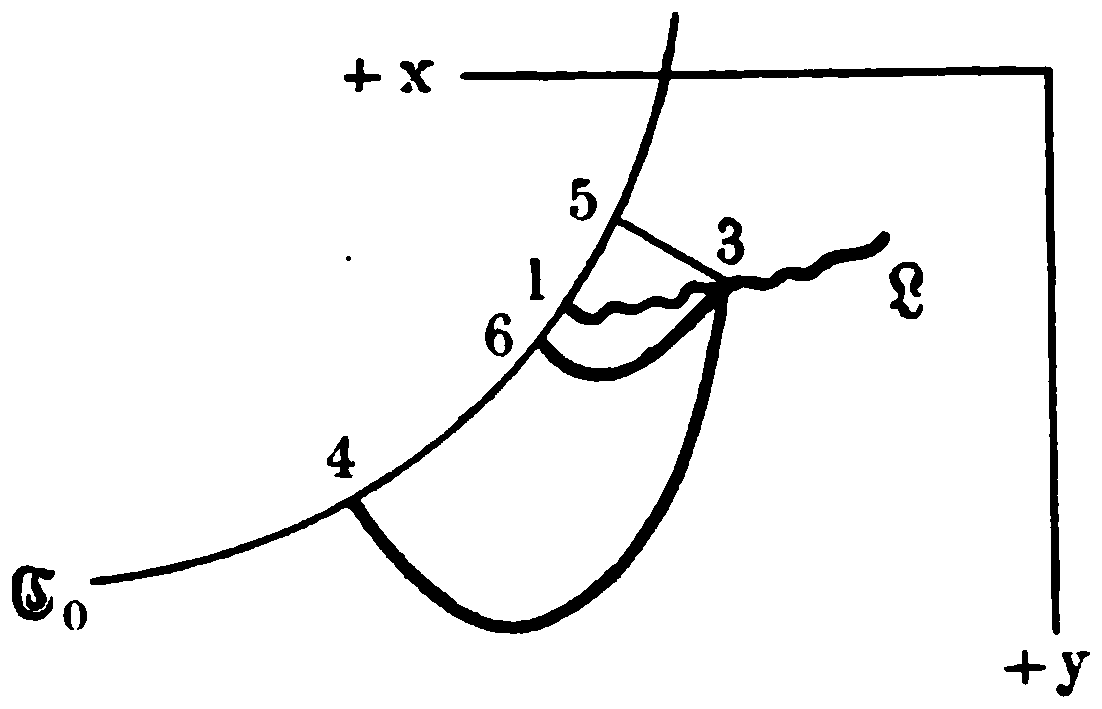
\includegraphics[width=\linewidth,height=35mm,keepaspectratio]{figures/fig18_accepted_derivative.png}\par\vspace{1mm}
\end{minipage}
\end{center}
% src-pdfpage=0177
% src-break=0177
曲线 $\mathfrak{C}_0$ 使点 6 从 4 移动到 5，那么该点从不垂直地在 3 的上方或下方，其法线始终在点 3 之下穿过。因此，总可以构造一条与曲线 $\mathfrak{C}_0$ 垂直相交的向下凸的极值曲线 36，对于其长度 $\mathfrak{R}_{36}$，当 $\mathfrak{R}_{35}$ 为直线距离 35 时，不等式

\[
\mathfrak{R}_{36}>\mathfrak{R}_{35}
\]
成立，且 $\mathfrak{R}_{36}-\mathfrak{R}_{35}$ 可以任意小。显然，现在

\[
K_{13}\geq \mathfrak{R}_{35},
\]
因此，根据不等式（34），至少对于点 6 的一个位置，有

\[
K_{13}=\mathfrak{R}_{36},
\]
由此，魏尔斯特拉斯的构造首先对弧$\Omega_1$得以实施。对于曲线$\Omega$的其余部分，其可能性由\S~38得出，只要以该处所给的方式进行变分；因为在此处，只要满足雅可比对链线02的条件，量$\Delta$便不再消失。曲线$\Omega$以与$\mathfrak{C}_0$正交的直线段开始的情况，也可以像上面问题IX那样同样容易地处理。

% machine-unit: Kneser_LVR_DE_p0177low_p0192 §§40-42
% appended in continuation package p0177-p0192; §43 excluded.
% src-pdfpage=0177
% src-break=0177-partial-lower
\begin{center}
{\large \S~40.}
\end{center}
以下推导适用于两种情况，无论场中的极值曲线是否具有固定点 0，或者是否在可变点 0 处以横截方式与固定曲线 $\mathfrak{C}_0$ 相交。

沿着弧线 $\mathfrak{C}$ 从位于其上的点 0 出发移动时，量 $\Delta$ 首次在点 1 处消失，且对于这样的参数 $t=t_1$，在位置 $(t_1,a_0,b_0)$ 处函数 $\xi,\eta,\omega$ 是正则的，且量 $\xi_t,\eta_t$ 并非同时消失。那么在上述区分的两种情况中，点 1 在第一种情况下被称为与点 0 共轭，在第二种情况下被称为曲线 $\mathfrak{C}_0$ 的极值焦点，对于当前的问题，具有特征性质

\begin{equation}\tag{35}
\Delta(t_1,a_0,b_0)=0.
\end{equation}
于是，\S~36 中围绕方程（10）、（11）所作的推演说明了如何构造曲线 01，并使沿该曲线

% src-pdfpage=0178
% src-break=0178
魏尔斯特拉斯构造可行，而量 $\mathfrak{E}$ 处处消失，因而方程

\begin{equation}\tag{36}
\bar J_{01}=J_{01},\quad \bar K_{01}=K_{01}
\end{equation}
得出，从而使极值终止。为此，首先将 $t$ 作为 $a$ 和 $b$ 的函数，通过方程

\begin{equation}\tag{37}
\Delta(t,a,b)=0
\end{equation}
定义；我们假设，它是

\[
\Delta_t(t_1,a_0,b_0)\gtrless 0,
\]
因此，考虑到方程（35），对于$t$得出一个表达式

\[
t=t_1+[a-a_0,b-b_0]_1.
\]
我们进一步设定微分方程

\[
\left|\begin{array}{cc}
\xi_tdt+\xi_a da+\xi_b db&\eta_tdt+\eta_a da+\eta_b db\\[.6ex]
\xi_t&\eta_t
\end{array}\right|=0
\]
或者

\begin{equation}\tag{38}
(\xi_t\eta_a-\xi_a\eta_t)\,da+(\xi_t\eta_b-\xi_b\eta_t)\,db=0
\end{equation}
，并把所得的 $t$ 表达式代入其中；于是 $da$ 和 $db$ 的因子是关于自变量 $a-a_0$, $b-b_0$ 的幂级数。如果作如下假设，那么它们在 $a=a_0$, $b=b_0$ 时不会同时消失：矩阵

\begin{equation}\tag{39}
\begin{array}{ccc}
\xi_t&\xi_a&\xi_b\\
\eta_t&\eta_a&\eta_b
\end{array}
\end{equation}
的二阶行列式对于值组 $t=t_1$, $a=a_0$, $b=b_0$ 并非全都消失。如果那两个因子确实为零，那么矩阵的第三个行列式也将为零，因为 $\xi_t$ 和 $\eta_t$ 并非同时消失。因此，当 $a_0$ 和 $b_0$ 相对应时，方程（38）将给出一种形式的关系

\[
b-b_0=[a-a_0]_1,\quad a-a_0=[b-b_0]_1.
\]
例如，若成立第一个方程，并将所得的 $b$ 和 $t$ 的值代入方程

\begin{equation}\tag{40}
x=\xi(t,a,b),\quad y=\eta(t,a,b),
\end{equation}
所以 $x$ 和 $y$ 以 $[a-a_0]_0$ 的形式出现，对于 $a=a_0$ 特别地

\[
x=x_1,\quad y=y_1.
\]
因此，方程（40）表示一条经过点 1 的曲线 $\mathfrak{C}$；在该点附近，除

% src-pdfpage=0179
% src-break=0179
点 1 本身外，该曲线正则。若点 1 是一个回返点，则对它应有方程

\[
\xi_tdt+\xi_a da+\xi_b db=0,\quad \eta_tdt+\eta_a da+\eta_b db=0;
\]
现在方程

\[
\Delta_tdt+\Delta_a da+\Delta_b db=0
\]
成立，并且如果大小 $\dfrac{db}{da}$ 和 $\dfrac{da}{db}$ 中有一个不等于零，那么就会得出

\begin{equation}\tag{41}
\frac{\partial(\xi,\eta,\Delta)}{\partial(t,a,b)}=0.
\end{equation}
因此，如果这个方程对于$t=t_1$、$a=a_0$、$b=b_0$不成立，那么曲线$\mathfrak{C}$在点1处就没有回转点。

由方程（38）可知，由于$\xi_t$和$\eta_t$不同时为零，因此可以设：

\begin{equation}\tag{42}
\xi_tdt+\xi_a da+\xi_b db=m\xi_tdt,\quad
\eta_tdt+\eta_a da+\eta_b db=m\eta_tdt;
\end{equation}
因此，曲线 $\mathfrak{C}$ 在每一点都与属于同一值组 $(a,b)$ 的极值曲线（40）相切，并且是这些曲线的某个单参数无限族的包络线。

根据方程（37）以及关于系统（39）所引入的假设，从方程（42）可以得出

\[
\omega_tdt+\omega_a da+\omega_b db=m\omega_tdt,
\]
或者，显然

\[
\omega_t=G(\xi,\eta,\xi_t,\eta_t)
\]
可以被设定，

\[
\omega_tdt+\omega_a da+\omega_b db=mG(\xi,\eta,\xi_t,\eta_t)dt.
\]
现在，如果 $mdt$ 为正，则由于函数 $G$ 和方程 (42) 的齐次性，可以从中得出结论

\[
\omega_tdt+\omega_a da+\omega_b db
=G(\xi,\eta,\xi_tdt+\xi_a da+\xi_b db,\eta_tdt+\eta_a da+\eta_b db).
\]
微分 $dt,da,db$ 均与沿曲线 $\mathfrak{C}$ 的进展有关；若将与该进展相应的增量记为 $D$，则可将最后一个方程和方程（42）写成

\[
Dx=m\xi_tdt,
\quad Dy=m\eta_tdt,
\quad D\omega=G(\xi,\eta,Dx,Dy).
\]
% src-pdfpage=0180
% src-break=0180
因此，当未带划线的积分符号 $K$ 作用于曲线 $\mathfrak{C}$ 时，且 3 是该曲线上的一个点（图~19），由方程可得

\[
DK_{31}=-G(x,y,Dx,Dy)
\]
在 $mdt>0$ 时可得

\begin{equation}\tag{43}
D\omega+DK_{31}=D(\bar K_{03}+K_{31})=0,
\end{equation}
其中带横线的 $K$ 指的是通过与点 3 相关的值组 $(a,b)$ 所定义的那条极值曲线 03。因此，这些极值曲线为曲线 $\mathfrak{C}$ 提供了魏尔斯特拉斯的构造，而量

\[
\mathfrak{E}(x,y,x',y',Dx,Dy)=\mathfrak{E}(x,y,\xi_t,\eta_t,Dx,Dy)
\]
在 $mdt$ 为正时以通常方式消失。

\begin{center}
{\small 图~19.}\par\vspace{1mm}
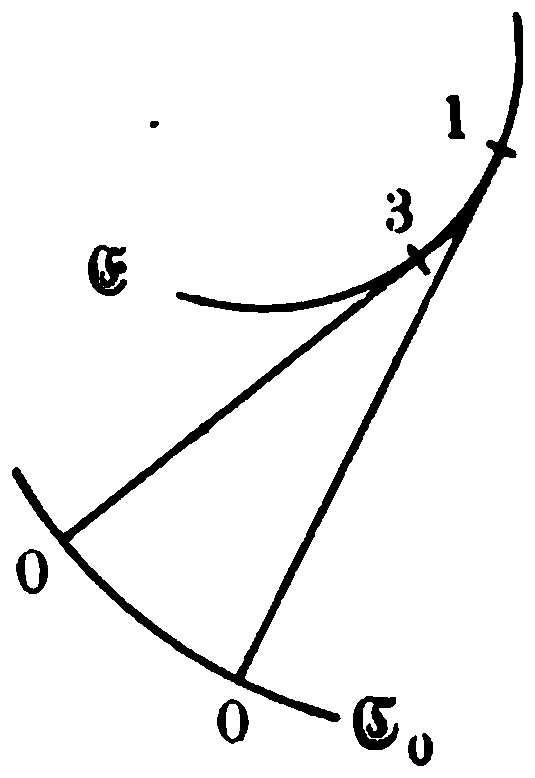
\includegraphics[width=.34\linewidth,height=55mm,keepaspectratio]{figures/fig19_accepted_derivative.png}
\end{center}
由此可以推导出方程（36），符号 $D$ 必须表示在曲线 $\mathfrak{C}$ 上朝向点 1 的方向。这一方向可能与在点 3 相切的极值曲线上的 $t$ 增大方向一致，也可能不一致。当曲线 $\mathfrak{C}$ 在点 1 处有一个回返点，从该点出发，曲线的两个分支都朝向随着 $t$ 增大而经过的曲线 $\mathfrak{C}$ 的方向时，就会出现后一种情况；如果这两个分支的方向相反，或者根本不存在回返点，那么在曲线 $\mathfrak{C}$ 在点 1 附近被该点分割成的至少一个半段中，曲线 $\mathfrak{C}$ 朝向点 1 的方向将与极值曲线 03 上 $t$ 值增大的方向一致；这个半段将用 $\mathfrak{C}_1$ 表示。后者方向由值对

\[
x'=\xi_t,
\quad y'=\eta_t
\]
定义；因此，在半段 $\mathfrak{C}_1$ 上，$Dx$ 与 $\xi_t$、$Dy$ 与 $\eta_t$ 分别只相差一个正因子，于是 $mdt$ 为正，从而上述量 $\mathfrak{E}$ 消失。只要方程（41）不成立、从而排除了回返点，就必定存在这样的弧 $\mathfrak{C}_1$。

现在，设 3 是弧 $\mathfrak{C}_1$ 上任意接近点 1 的一点；则上面构造的极值曲线 03
% END PHYSICALLY EMBEDDED BODY INH04 3/5
% BEGIN PHYSICALLY EMBEDDED BODY INH04 4/5: inherited/INH04_pdf151_200_producer_r2/work/zh_181_190.tex
% src-pdfpage=0181
% src-break=0181
与曲线 $\mathfrak{C}_1$ 的弧 31 构成一个具有连续变化切线的连续线段，该线段与属于曲线 $\mathfrak{C}$ 的弧 01 的偏差可以任意小，并且在两个线段的邻近点上，切线也仅略有不同。在此过程中，必须满足方程

\[
d(\bar J_{03}+J_{31})=\mathfrak{E}(x,y,x',y',Dx,Dy)=0;
\]
因为上面推导出的 $\bar J_{03}$ 和 $J_{31}$ 的偏微分商表达式，在位置 $(t_1,a_0,b_0)$ 的附近也仍然有效，因为所提到的积分在这里也是 $t,a,b$ 的正规函数。从得到的和魏尔斯特拉斯的构造特征方程（43）可以得出

\[
\bar J_{03}+J_{31}=\bar J_{01},
\quad \bar K_{03}+K_{31}=\bar K_{01}.
\]
因此，曲线 $\mathfrak{C}$ 的弧 01 不再给出积分 $J$ 的极值；这里比较的是所有使积分 $K$ 取相同值的曲线。相反，由于折线 031 具有上述性质，弱极值在点 1 就已经终止。

\noindent\textbf{例。问题九} 按如下方式具体化：从一个角的一条边上的给定点出发，在该角的凸侧向另一条边作一条给定长度的线，使它与两条边围成尽可能大的面积。

第二条边为直线 $y=0$；所要极值化的面积与积分 $\int yx' dt$ 只相差一个常数三角形面积，该三角形面积是由给定点向第二条边所作的垂线从角中截取的。与直线 $y=0$ 横截相交的极值曲线，在该直线上 (\S~34) 垂直，并且是圆，因此可由方程

\begin{equation}\tag{44}
x=a+b\cos t,
\quad y=b\sin t
\end{equation}
表示；对于点 0，总是 $t=0$，因此

\[
\bar K_{03}=\omega(t,a,b)=bt.
\]
由此得出

\[
\Delta=\begin{vmatrix}
-b\sin t&b\cos t&b\\
1&0&0\\
\cos t&\sin t&t
\end{vmatrix}=b(\sin t-t\cos t);
\]
% src-pdfpage=0182
% src-break=0182
因此，在每个同直线 $y=0$ 正交的圆上，该直线的极值焦点由下列方程的最小根确定：

\[
\tg t=t
\]
把该根记作 $t_1$，其近似值为

\[
t_1=\frac{257\frac{1}{2}}{360}\cdot 2\pi
\]
即对应于角 $257\frac{1}{2}^{\circ}$ 。提供定义曲线 $\mathfrak{C}$ 的关系的方程（38）将简化为

\[
b\,db+b\cos t_1\,da=0,
\quad db+\cos t_1\,da=0.
\]
这样的 $a$ 与 $b$ 之间的关系，从圆的二参数无限族（44）中选出一个与两条固定直线相切的单参数无限族；若 $\alpha$ 是这两条固定直线所成的凹角，则

\[
\sin\frac{\alpha}{2}=-\cos t_1=\cos(t_1-\pi),
\quad \frac{\alpha}{2}=\frac{3\pi}{2}-t_1=12\frac{1}{2}^{\circ}.
\]
在这族曲线中，极值的终止可以用初等方法清楚地展示（图~20）。事实上，若1、3是位于角$\alpha$同一边上的两点，且3比1更靠近顶点，若进一步设$0_0,0$是通过1、3的该族圆与角$\alpha$的角平分线的交点，且弧$10_0$、30的圆心角为$t_1$，则弧$10_0$与复合线130的长度相等；若从1向角$\alpha$的角平分线作垂线14，则水平斜线区域$10_0 41$和

\begin{center}
{\small 图~20.}\par\vspace{1mm}
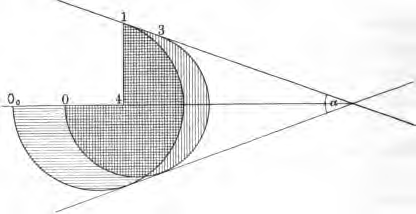
\includegraphics[width=.70\linewidth,height=40mm,keepaspectratio]{figures/fig20_accepted_derivative.png}
\end{center}
% src-pdfpage=0183
% src-break=0183
垂直的阴影区域13041具有相同的面积，使得弧$10_0$显然不能在给定弧长的情况下提供面积的极值。弧$\mathfrak{C}_1$是直线段13。

\begin{center}
{\large \S~41.}
\end{center}
选取极值曲线 $\mathfrak{C}$ 上的点 0，使 $\xi_t$ 不为零；于是极值曲线的微分方程可写成

\[
f_y+\lambda g_y-\frac{d(f_p+\lambda g_p)}{dx}=0
\]
；由此得到 $\dfrac{dp}{dx}$ 的一个关于 $x,y,p$ 的正则表达式，只要不等式

\begin{equation}\tag{45}
f_{pp}+\lambda g_{pp}\gtrless 0
\end{equation}
成立。在此前提下，\S~27 的一般定理表明，该微分方程有如下形式的积分

\begin{equation}\tag{46}
y=\Phi(x,a,b,\lambda)
\end{equation}
；当 $a=a_0$、$b=b_0$、$\lambda=\lambda_0$ 时，该积分给出曲线 $\mathfrak{C}$，并且在位置 $(x_{00},a_0,b_0,\lambda_0)$ 处正则，其中以 $x_{00}$ 表示点 0 的横坐标。特别地，若为 $a$ 和 $b$ 分别取 $y$ 和 $p$ 在 $x=x_{00}$ 时的值，则有

\[
\Phi(x,a,b,\lambda)=a+b(x-x_{00})+[x-x_{00}]_2
\]
和对于 $x=x_{00}$ 是

\begin{equation}\tag{47}
\Phi_b=0,
\quad \Phi_{bx}=1.
\end{equation}
我们现在要从方程（46）给出的三参数极值曲线族中选出一个二参数子族，使其横截一条从点 0 出发的正则曲线 $\mathfrak{C}_0$；后者的方程为

\[
y_0=\gamma(x_0)
\]
。满足下列方程时即可做到：

\begin{equation}\tag{48}
\begin{aligned}
M&=\Phi(x_0,a,b,\lambda)-\gamma(x_0)=0,\\
N&=f+\lambda g-p(f_p+\lambda g_p)+(f_p+\lambda g_p)\gamma'(x)\big|_{x=x_0}=0;
\end{aligned}
\end{equation}
% src-pdfpage=0184
% src-break=0184
这里，在第二个方程中应把 $y$ 和 $p$ 分别换成 $\Phi$ 和 $\Phi_x$。这些方程的左端在位置 $x_0=x_{00}$、$a=a_0$、$b=b_0$、$\lambda=\lambda_0$ 正则；很容易看出，何时可以由它们把量 $x,a,b,\lambda$ 中的两个表示为其余量的函数。事实上，构成

\[
\frac{\partial(M,N)}{\partial(x_0,b)}=
\left|\begin{array}{cc}
\Phi_x-\gamma'(x)&\Phi_b\\[.6ex]
\dfrac{\partial N}{\partial x}+\Phi_x\dfrac{\partial N}{\partial y}+\Phi_{xx}\dfrac{\partial N}{\partial p}&
\dfrac{\partial N}{\partial y}\Phi_b+\dfrac{\partial N}{\partial p}\Phi_{bx}
\end{array}\right|_{x=x_0}
\]
并注意到显然有

\[
\frac{\partial N}{\partial p}=[\gamma'(x)-\Phi_x](f_{pp}+\lambda g_{pp})\big|_{x=x_0},
\]
则根据方程（47），对于 $x=x_{00}$ 得到

\[
\frac{\partial(M,N)}{\partial(x_0,b)}=-[\gamma'(x)-\Phi_x]^2(f_{pp}+\lambda g_{pp})\big|_{x=x_{00}}
\]
并且这个表达式在位置 $(x_{00},a_0,b_0,\lambda_0)$ 处不等于零，当

\[
\Phi_x(x_{00},a_0,b_0,\lambda_0)-\gamma'(x_{00})\gtrless 0,
\]
即曲线 $\mathfrak{C}$ 与 $\mathfrak{C}_0$ 不相切时。于是，方程（48）给出 $b-b_0$ 和 $x_0-x_{00}$ 的如下形式的表达式

\[
[a-a_0,\lambda-\lambda_0]_1;
\]
将前者代入 $\Phi$ 以代替 $b-b_0$，则可得到一个表达式

\begin{equation}\tag{49}
y=\varphi(x,a,\lambda),
\end{equation}
它在位置 $(x_{00},a_0,\lambda_0)$ 正则，并定义一个与 $\mathfrak{C}_0$ 横截相交的二参数无限极值曲线族。若曲线 $\mathfrak{C}_0$ 收缩为点 0，则得到同一结果；也就是说，只需把方程

\begin{equation}\tag{50}
\Phi(x_{00},a,b,\lambda)-y_{00}=0
\end{equation}
关于 $b$ 解出，便得到通过该点的极值曲线方程。

在每一种情形中，量 $a,b,\lambda$ 之间都由方程

\begin{equation}\tag{51}
\Omega(a,b,\lambda)=0
\end{equation}
建立一种关系，并且该方程满足

% src-pdfpage=0185
% src-break=0185
\begin{equation}\tag{52}
\Omega_b(a_0,b_0,\lambda_0)\gtrless 0
\end{equation}
，且其左端在位置 $(a_0,b_0,\lambda_0)$ 的邻域内正则。显然有

\[
\Omega_a+\Omega_b\frac{\partial b}{\partial a}=0,
\quad
\Omega_\lambda+\Omega_b\frac{\partial b}{\partial \lambda}=0,
\]
\[
\varphi_a(x,a,\lambda)=\Phi_a+\Phi_b\frac{\partial b}{\partial a},
\quad
\varphi_\lambda(x,a,\lambda)=\Phi_\lambda+\Phi_b\frac{\partial b}{\partial\lambda},
\]
并且类似的方程适用于每一个首先作为 $a,b,\lambda$ 的函数出现，然后仅转变为 $a$ 和 $\lambda$ 的函数的量。

例如，设

\[
\Theta(x,a,b,\lambda)=\int_{x_0}^{x}g(x,\Phi,\Phi_x)\,dx
\]
若该量在假设（51）下化为 $\omega(x,a,\lambda)$，那么由于可以令 $t=x$，它对于极值曲线（49）具有与先前的量 $\omega(t,a,b)$ 相同的意义；在 $\Delta$ 中把 $b$ 替换为 $\lambda$，便得到下式：

\[
\begin{aligned}
\Delta&=\frac{\partial(\xi,\eta,\omega)}{\partial(x,a,\lambda)}
=\frac{\partial(\varphi,\omega)}{\partial(a,\lambda)} \\
&=\begin{vmatrix}
\Phi_a+\Phi_b\dfrac{\partial b}{\partial a}&\Phi_\lambda+\Phi_b\dfrac{\partial b}{\partial\lambda}\\[1.0ex]
\Theta_a+\Theta_b\dfrac{\partial b}{\partial a}&\Theta_\lambda+\Theta_b\dfrac{\partial b}{\partial\lambda}
\end{vmatrix}\\
&=\frac{1}{\Omega_b}\begin{vmatrix}
\Phi_a&\Phi_b&\Phi_\lambda\\
\Omega_a&\Omega_b&\Omega_\lambda\\
\Theta_a&\Theta_b&\Theta_\lambda
\end{vmatrix}=\frac{D}{\Omega_b}.
\end{aligned}
\]
如果能够证明这个行列式并不恒等于零，那么就表明极值曲线 $y=\varphi(x,a,\lambda)$ 至少在点 0 的邻域内按照 \S~39 的意义形成一个场。

为了研究最近获得的行列式，我们假设 $x_0$ 作为 $a,b,\lambda$ 的正则函数来定义；因此我们有方程

\[
\Theta_a=-g\frac{\partial x_0}{\partial a}\bigg|^0+\int_{x_0}^{x}\frac{\partial g}{\partial a}\,dx
=-g\frac{\partial x_0}{\partial a}\bigg|^0+g_p\Phi_a\bigg|_{x_0}^{x}+\int_{x_0}^{x}\left(g_y-\frac{dg_p}{dx}\right)\Phi_a\,dx
\]
% src-pdfpage=0186
% src-break=0186
连同类似的，其中 $a$ 被 $b$ 或 $\lambda$ 替代。由此可得

\[
D=\frac{\partial(\Phi,\Omega,\Theta)}{\partial(a,b,\lambda)}
\]
\[
=\begin{vmatrix}
\Phi_a&\Phi_b&\Phi_\lambda\\[.6ex]
\Omega_a&\Omega_b&\Omega_\lambda\\[.6ex]
A+\displaystyle\int_{x_0}^{x}\left(g_y-\frac{dg_p}{dx}\right)\Phi_a\,dx&B+\displaystyle\int_{x_0}^{x}\left(g_y-\frac{dg_p}{dx}\right)\Phi_b\,dx&C+\displaystyle\int_{x_0}^{x}\left(g_y-\frac{dg_p}{dx}\right)\Phi_\lambda\,dx
\end{vmatrix},
\]
其中量 $A,B,C$ 与 $x$ 相互独立；因为表达式 $\Theta_a,\Theta_b,\Theta_\lambda$ 中在积分符号前的项，这些项依赖于 $x$，当用 $g_p$ 乘以行列式的第一行并从最后一行减去时，这些项就会消失。如果此时表达式 $D$ 恒等于零，那么首先，矩阵

\begin{equation}\tag{53}
\left\|\begin{array}{ccc}
\Omega_a&\Omega_b&\Omega_\lambda\\[.8ex]
A+\displaystyle\int_{x_0}^{x}\cdots&B+\displaystyle\int_{x_0}^{x}\cdots&C+\displaystyle\int_{x_0}^{x}\cdots
\end{array}\right\|
\end{equation}
的全部二阶行列式可以同时恒等消失。它们对 $x$ 的微分商是该矩阵的行列式

\[
\left\|\begin{array}{ccc}
\Omega_a&\Omega_b&\Omega_\lambda\\[.8ex]
\left(g_y-\dfrac{dg_p}{dx}\right)\Phi_a&
\left(g_y-\dfrac{dg_p}{dx}\right)\Phi_b&
\left(g_y-\dfrac{dg_p}{dx}\right)\Phi_\lambda
\end{array}\right\|;
\]
现在在曲线 $\mathfrak{C}$ 上作为相对极值问题的极值曲线，量

\[
R=g_y-\frac{dg_p}{dx}
\]
不消失，那么矩阵

\[
\left\|\begin{array}{ccc}
\Omega_a&\Omega_b&\Omega_\lambda\\
\Phi_a&\Phi_b&\Phi_\lambda
\end{array}\right\|
\]
的各行列式也都会消失，例如

\begin{equation}\tag{54}
\Omega_a\Phi_b-\Omega_b\Phi_a=0,
\quad
\Omega_\lambda\Phi_b-\Omega_b\Phi_\lambda=0.
\end{equation}
这些方程中的第一个显然是不可能的，因为对于 $x=x_{00}$, $a=a_0$, $b=b_0$, $\lambda=\lambda_0$

% src-pdfpage=0187
% src-break=0187
\begin{equation}\tag{55}
\Phi_a=1,
\quad \Phi_b=0,
\quad \Omega_b\gtrless 0;
\end{equation}
第二个方程也不可能成立，因为 $\Phi_b$ 以一次幂开始，而 $\Phi_\lambda$ 以 $x-x_{00}$ 的更高次幂开始；量 $\Phi_\lambda$ 不可能恒等于零，否则表达式 $\Phi$ 将与 $\lambda$ 无关，因而也会满足方程

\[
f_y-\frac{df_p}{dx}=0
\]
；而该方程的左边同 $R$ 一样，在曲线 $\mathfrak{C}$ 上不等于零。

特别由此推得，这些行列式中没有一个

\begin{equation}\tag{56}
\left|\begin{array}{cc}
\Omega_a&\Omega_b\\[.8ex]
A+\displaystyle\int_{x_0}^{x}R\Phi_a\,dx&B+\displaystyle\int_{x_0}^{x}R\Phi_b\,dx
\end{array}\right|,
\quad
\left|\begin{array}{cc}
\Omega_\lambda&\Omega_b\\[.8ex]
C+\displaystyle\int_{x_0}^{x}R\Phi_\lambda\,dx&B+\displaystyle\int_{x_0}^{x}R\Phi_b\,dx
\end{array}\right|
\end{equation}
恒等于零，因为它们的导数是方程（54）左边的表达式，乘以不为零的量 $R$。根据行列式理论的一个一般定理，消失的行列式中，两行对应的余子式是成比例的；将这个定理应用于行列式 $D$ 的第一行和第三行，可以得出最后两个行列式与方程（54）左边的表达式成比例。现在，这四个量中没有一个恒等于零，而且量 $R$ 也不为零，因此得出量（56）对 $x$ 的对数导数相等，这些量本身因此处于如下关系：

\[
\left|\begin{array}{cc}
\Omega_a&\Omega_b\\[.8ex]
A+\displaystyle\int_{x_0}^{x}R\Phi_a\,dx&B+\displaystyle\int_{x_0}^{x}R\Phi_b\,dx
\end{array}\right|
=M
\left|\begin{array}{cc}
\Omega_\lambda&\Omega_b\\[.8ex]
C+\displaystyle\int_{x_0}^{x}R\Phi_\lambda\,dx&B+\displaystyle\int_{x_0}^{x}R\Phi_b\,dx
\end{array}\right|
\]
% src-pdfpage=0188
% src-break=0188
成立，当通过 $M$ 表示一个与 $x$ 无关的、有限的且不为零的量时。由此，通过考虑量 $R$ 不为零的值进行微分，可得出结论。

\[
\Omega_a\Phi_b-\Omega_b\Phi_a=M(\Omega_\lambda\Phi_b-\Omega_b\Phi_\lambda).
\]
在这里令 $x=x_{00}$，左边便化为 $-\Omega_b$，而因关系式（55）成立，右边为零。因此，假设 $D$ 恒等于零总会导致矛盾。

根据 $D$ 与 $\Delta$ 的关系，至此证明了如下结论。若在此前关于极值曲线 $\mathfrak{C}$ 的假设中再加入不等式（45），那么从点 0 开始的弧总可以由一个场包围；该场的极值曲线要么全都通过点 0，要么横截一条给定的、在点 0 被曲线 $\mathfrak{C}$ 横截而不相切的正则曲线 $\mathfrak{C}_0$。因此，对于足够短的极值曲线弧，无论所求曲线的一个端点还是两个端点被固定，极值的雅可比条件都成立。

\begin{center}
{\large \S~42.}
\end{center}
如果点 0 是固定的，并且根据这一情况用特殊的关联式（50）代替方程 $\Omega=0$，那么就有

\[
\Omega_a=\Phi_a(x_0,a,b,\lambda),
\]
\[
\Omega_b=\Phi_b(x_0,a,b,\lambda),
\quad
\Omega_\lambda=\Phi_\lambda(x_0,a,b,\lambda)
\]
因此获得

\[
D=\frac{\partial\left\{\Phi(x,a,b,\lambda),\ \Phi(x_0,a,b,\lambda),\ \displaystyle\int_{x_0}^{x}g[x,\Phi(x,a,b,\lambda),\Phi_x(x,a,b,\lambda)]\,dx\right\}}{\partial(a,b,\lambda)}.
\]
由于该表达式的值为

\[
\Delta\Phi_b(x_0,a,b,\lambda)
\]
，故量

\[
\Delta(x_0,x)=D\big|_{a=a_0,\,b=b_0,\,\lambda=\lambda_0}
\]
% src-pdfpage=0189
% src-break=0189
当点 0 和 $(x,y)$ 共轭时消失。由此导出了迈尔提出的共轭点的特征标志。魏尔斯特拉斯的类似公式则是在假设极值曲线由下式表示时得到的：

\begin{equation}\tag{57}
x=X(t,a,b,\lambda),
\quad y=Y(t,a,b,\lambda)
\end{equation}
此时有恒等式

\[
Y=\Phi(X,a,b,\lambda)
\]
并且由此得出的那些关系

\[
\begin{gathered}
Y_t=\Phi_x(X,a,b,\lambda)X_t,
\quad Y_a=\Phi_xX_a+\Phi_a,
\quad Y_b=\Phi_xX_b+\Phi_b,\\
Y_\lambda=\Phi_xX_\lambda+\Phi_\lambda;
\end{gathered}
\]
\[
X_t\Phi_a=X_tY_a-X_aY_t=\theta_1(t),
\]
\[
X_t\Phi_b=X_tY_b-X_bY_t=\theta_2(t),
\quad
X_t\Phi_\lambda=X_tY_\lambda-X_\lambda Y_t=\theta_3(t).
\]
因此，若点 0 属于参数 $t=t_0$，则得出

\[
D X_t(t,a,b,\lambda)X_t(t_0,a,b,\lambda)=
\begin{vmatrix}
\theta_1(t)&\theta_2(t)&\theta_3(t)\\
\theta_1(t_0)&\theta_2(t_0)&\theta_3(t_0)\\[.6ex]
\dfrac{\partial K}{\partial a}&\dfrac{\partial K}{\partial b}&\dfrac{\partial K}{\partial\lambda}
\end{vmatrix},
\]
其中设定为

\[
K=\int_{x_0}^{x}g\,dx=\int_{t_0}^{t}G(X,Y,X_t,Y_t)\,dt.
\]
现在由于 $x_0$ 不依赖于 $a,b,\lambda$，我们有方程

\[
\frac{\partial K}{\partial a}=\Phi_a g_p\bigg|_{x_0}^{x}+\int_{x_0}^{x}\Phi_a\left(g_y-\frac{dg_p}{dx}\right)dx
\]
连同类似公式，其中 $a$ 被 $b$ 和 $\lambda$ 替代；因此，在行列式 $D$ 中，将前几行乘以适当的因子后加到最后一行，该行将变为：

\[
\int_{x_0}^{x}\Phi_a\left(g_y-\frac{dg_p}{dx}\right)dx,
\quad
\int_{x_0}^{x}\Phi_b\left(g_y-\frac{dg_p}{dx}\right)dx,
\quad
\int_{x_0}^{x}\Phi_\lambda\left(g_y-\frac{dg_p}{dx}\right)dx.
\]
进一步地，根据 \S~5，当

\[
G(x,y,x',y')=x'g\left(x,y,\frac{y'}{x'}\right)
\]
被引入

% src-pdfpage=0190
% src-break=0190
\[
x'\left(g_y-\frac{dg_p}{dx}\right)=G_y-G'_{y'}=-\frac{x'}{y'}(G_x-G'_{x'});
\]
由此可得

\[
\Phi_a\left(g_y-\frac{dg_p}{dx}\right)dx=\biggl(Y_a-X_a\frac{Y_t}{X_t}\biggr)(G_y-G'_{y'})dt
\]
\[
=[X_a(G_x-G'_{x'})+Y_a(G_y-G'_{y'})]dt.
\]
因此，设

\[
\Theta_1(t_0,t)=\int_{t_0}^{t}dt\,[X_a(G_x-G'_{x'})+Y_a(G_y-G'_{y'})]
\]
并由此产生 $\Theta_2$ 和 $\Theta_3$，通过将 $a$ 替换为 $b$ 和 $\lambda$，从而得到魏尔斯特拉斯行列式

\[
D X_t(t,a,b,\lambda)X_t(t_0,a,b,\lambda)=
\begin{vmatrix}
\theta_1(t)&\theta_2(t)&\theta_3(t)\\
\theta_1(t_0)&\theta_2(t_0)&\theta_3(t_0)\\
\Theta_1(t_0,t)&\Theta_2(t_0,t)&\Theta_3(t_0,t)
\end{vmatrix}=D(t_0,t).
\]
在此需要注意的是，$D$ 仅在以下假设下才有定义：在区间 $t_0\ldots t$ 内，处处 $y$ 作为 $x$ 的正则函数，由曲线 $\mathfrak{C}$ 所定义。而右边则对于每一个弧 $\mathfrak{C}$ 都有意义，沿着该弧 $x$ 和 $y$ 是 $t$ 的正则函数，并且量 $H_1(x,y,x',y')$ 不消失；因为根据 \S~27，这样的弧总是可以嵌入到由方程（57）所表示的曲线族中。

如果 $D(t_0,t)$ 不恒等于零，那么至少有一个量 $\theta_1(t_0),\theta_2(t_0),\theta_3(t_0)$ 不等于零。假设是最后一个；那么 $t_0$ 和 $\lambda$ 可以从方程中解出

\[
x_0=X(t_0,a,b,\lambda),
\quad y_0=Y(t_0,a,b,\lambda)
\]
作为 $a$ 和 $b$ 的正规函数被计算出来；代入它们，就得到

\[
X=\xi(t,a,b),
\quad Y=\eta(t,a,b).
\]
然后下列方程成立：

\[
X_t\frac{\partial t_0}{\partial a}+X_\lambda\frac{\partial\lambda}{\partial a}+X_a\bigg|^{t_0}=Y_t\frac{\partial t_0}{\partial a}+Y_\lambda\frac{\partial\lambda}{\partial a}+Y_a\bigg|^{t_0}=0,
\]
\[
X_t\frac{\partial t_0}{\partial b}+X_\lambda\frac{\partial\lambda}{\partial b}+X_b\bigg|^{t_0}=Y_t\frac{\partial t_0}{\partial b}+Y_\lambda\frac{\partial\lambda}{\partial b}+Y_b\bigg|^{t_0}=0,
\]
% END PHYSICALLY EMBEDDED BODY INH04 4/5
% BEGIN PHYSICALLY EMBEDDED BODY INH04 5/5: inherited/INH04_pdf151_200_producer_r2/work/zh_191_200.tex
% src-pdfpage=0191
% src-break=0191
\[
\xi_t=X_t,
\quad \eta_t=Y_t,
\quad X_a+X_\lambda\frac{\partial\lambda}{\partial a}=\xi_a,
\quad Y_a+Y_\lambda\frac{\partial\lambda}{\partial a}=\eta_a,
\]
\[
X_b+X_\lambda\frac{\partial\lambda}{\partial b}=\xi_b,
\quad Y_b+Y_\lambda\frac{\partial\lambda}{\partial b}=\eta_b.
\]
由前四个方程可轻易得出

\[
\theta_1(t_0)+\theta_3(t_0)\frac{\partial\lambda}{\partial a}=\theta_2(t_0)+\theta_3(t_0)\frac{\partial\lambda}{\partial b}=0,
\]
从最后四个

\[
\theta_1(t)+\theta_3(t)\frac{\partial\lambda}{\partial a}=\xi_t\eta_a-\xi_a\eta_t,
\quad
\theta_2(t)+\theta_3(t)\frac{\partial\lambda}{\partial b}=\xi_t\eta_b-\xi_b\eta_t,
\]
并且大小 $\Theta$ 的定义得出

\[
\Theta_1(t_0,t)+\frac{\partial\lambda}{\partial a}\Theta_3(t_0,t)=
\int_{t_0}^{t}dt\{(G_x-G'_{x'})\xi_a+(G_y-G'_{y'})\eta_a\}=A,
\]
\[
\Theta_2(t_0,t)+\frac{\partial\lambda}{\partial b}\Theta_3(t_0,t)=
\int_{t_0}^{t}dt\{(G_x-G'_{x'})\xi_b+(G_y-G'_{y'})\eta_b\}=B.
\]
因此，在行列式 $D(t_0,t)$ 中将第三列与 $\partial\lambda:\partial a$ 和 $\partial\lambda:\partial b$ 相乘后加到第一列和第二列，便得到

\[
D(t_0,t)=-\theta_3(t_0)\begin{vmatrix}
\xi_t\eta_a-\xi_a\eta_t&\xi_t\eta_b-\xi_b\eta_t\\
A&B
\end{vmatrix}.
\]
既然根据 \S~35

\[
\omega_a=G_{x'}\xi_a+G_{y'}\eta_a+A,
\quad
\omega_b=G_{x'}\xi_b+G_{y'}\eta_b+B,
\]
\[
\omega_t=G=\xi_tG_{x'}+\eta_tG_{y'},
\]
于是终于得出

\[
D(t_0,t)=-\theta_3(t_0)\frac{\partial(\xi,\eta,\omega)}{\partial(t,a,b)}=-\theta_3(t_0)\Delta.
\]
在所引入的假设下，因此 $\Delta$ 和 $D(t_0,t)$ 只有同时消失，而方程

\[
D(t_0,t)=0
\]
只要方程左边不恒等于零，该方程就是参数 $t_0$ 与 $t$ 对应于共轭点的充要条件。因此，若量 $D(t_0,t)$ 除点 0 本身外在弧 02 上处处不为零，就会对每条弧 12 得到

% src-pdfpage=0192
% src-break=0192
所求类型的极值，其中弧 12 的起点可以任意接近 0，但不与 0 重合。

由此可得，根据在 \S~31 末尾所进行的讨论，对于端点固定的弧 12，极值的雅可比条件一般来说也可以这样表述：方程

\[
D(t_1,t)=0
\]
在路径12上除了$t=t_1$之外没有根；事实上，这一分析无需任何修改即可应用于现在由$D(t_0,t)$所表示的量，只要不等式

\[
\frac{\partial D(t_0,t)}{\partial t}\bigg|_{t=t_0}\gtrless 0
\]
成立。即使这些量

\[
d_\alpha(t_0)=\frac{\partial^\alpha D(t_0,t)}{\partial t^\alpha}\bigg|_{t=t_0}
\]
对于 $\alpha=1,2,\ldots n$ 完全消失，而 $d_{n+1}(t_1)$ 却不等于零的情况，只需要将 \S~31 的论证稍作修改，即让量 $d_{n+1}(t_0)$ 取代 $f_1(t_0)$ 即可。只有当 $d_{n+1}(t_0)$ 不完全消失，而 $d_{n+1}(t_1)$ 却具有零值时，才会怀疑是否可以应用上述的讨论。

% machine-manifest-begin
% {"work": "Kneser_LVR", "language": "de", "branch": "canonical_complete_volume", "source_pdf_pages": "author-clean cumulative p0011-p0335; sections 1-69, Literature, printed errata, and unnumbered addendum complete; p0336 rear board excluded by evidence ledger", "visible_text_policy": "authorial text only; no vendor marks, source captions, running heads, page numbers, signatures, or preservation/library notes", "math_policy": "all displayed and inline mathematical symbols retained as TeX; provenance appears only in comments and external ledgers", "figure_policy": "figures 1--24 retained as HQ source-derived whitened original crops only; no visible drawn/TikZ layer", "description": "complete diplomatic German edition", "completion_boundary": "source PDF335; PDF336 rear board excluded", "errata_policy": "printed errata transcribed as printed; body corrections not silently applied"}
% machine-manifest-end
% machine-unit: Kneser_LVR_DE_p0193_p0206 §§43-45
% src-pdfpage=0193
\begin{center}
{\large 第五章。}\\[1.1ex]
{\Large\bfseries 不连续解。}\\[2ex]
\rule{32mm}{0.4pt}\\[2ex]
{\large \S~43.}
\end{center}
前面各节的推导并不总是能给出原始极值问题的解，即在给定两点之间画出一条曲线，使得积分 $J$ 达到绝对或相对极值。只是表明，如果所求曲线应具有某些连续性性质，那么它只能是极值曲线的一个正则部分；随后在假设所求曲线的两个端点已经由一条不含奇点的极值曲线弧连接的情况下，导出了极值的条件。如果这一假设不成立，这在一些简单的问题中就已经出现，那么所求的极值就无法由具有上述连续性性质的曲线提供，于是就产生了这样一个问题：是否一条带有奇点，例如带有角点的曲线能够解决所给的问题。如果能够通过允许某些特定类型的奇点来回答这个问题，那么虽然还没有一种万无一失的方法来确定所求的极值，但能够解决该问题的情况范围却得到了扩展。

特别地，我们问，什么时候积分

\[
J=\int Fdt
\]
由一条包含有限多个在角点相接的

% src-pdfpage=0194
弧段的曲线使之取得绝对极值；每个弧段都具有先前对整条曲线所要求的性质。也就是说，沿每个弧段，$x$ 与 $y$ 都是参数 $t$ 的连续函数，并具有连续的一阶和二阶导数。对每个弧段，第二章的讨论仍然有效，因为可保持角点不变而把变分限制在弧段内部；所以每个弧段都必须是极值曲线的一段弧。

\begin{center}
{\small 图~21.}\par\vspace{1mm}
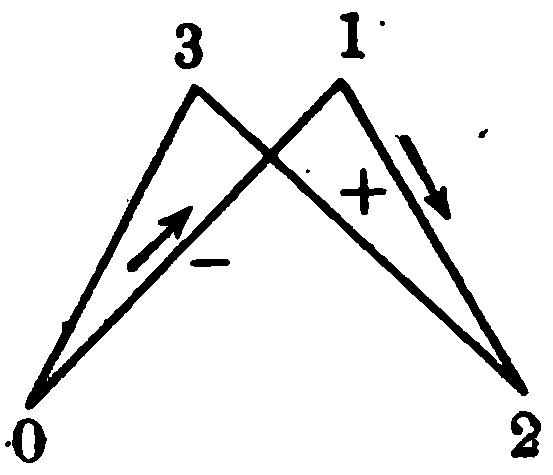
\includegraphics[width=.34\linewidth,height=33mm,keepaspectratio]{figures/fig21_accepted_derivative.png}
\end{center}
在角点1处相撞的弧段上，假设点0和点2足够接近角点，使得弧段01和12不包含共轭点对（图~21）。那么，点0和点2可以与每个足够接近点1的点3通过极值曲线03和32连接，而这些曲线可以按照\S~2作为弧段01和12的变分来考虑。因此，作为所求曲线的一部分的折线012，可以通过032来代替，因为根据\S~2的变分公式，对于01和02的每一部分仍然有效。现在设

\[
\delta x_1=x_3-x_1,\quad \delta y_1=y_3-y_1
\]
并按某个量是对弧 01 沿越过点 1 的方向形成，还是对弧 12 沿指向点 2 的方向形成，分别在该量的符号上加 $-$ 或 $+$，则有公式

\[
\Delta \overline{J}_{01}=F_{x'}^-\delta x+F_{y'}^-\delta y\big|^1+[\delta x_1,\delta y_1]_2,
\]
\[
\Delta \overline{J}_{12}=-F_{x'}^+\delta x-F_{y'}^+\delta y\big|^1+[\delta x_1,\delta y_1]_2,
\]
\[
F_{x'}^- =F_{x'}(x,y,x'_{-},y'_{-}),\quad
F_{x'}^+=F_{x'}(x,y,x'_{+},y'_{+}),\ldots,
\]
所以，相加后有

\[
\Delta\overline{J}_{012}=(F_{x'}^- -F_{x'}^+)\delta x+(F_{y'}^- -F_{y'}^+)\delta y\big|^1+[\delta x_1,\delta y_1]_2.
\]
若折线 012 所属的曲线要使积分 $J$ 取得极值，这个量就必须具有固定符号。因此，若角点 3 可在位置 1 附近自由移动，从而 $\delta x_1$、$\delta y_1$ 相互独立，则线性项的系数必须消失（\S~7），由此得到埃尔德曼定理。

% src-pdfpage=0195
\begin{equation}\tag{1}
F_{x'}^- =F_{x'}^+,
\quad F_{y'}^- =F_{y'}^+.
\end{equation}
相反，若预先把角点约束在曲线

\begin{equation}\tag{2}
h(x_1,y_1)=0
\end{equation}
上，使方程

\[
0=h_x(x_1,y_1)\delta x_1+h_y(x_1,y_1)\delta y_1+[\delta x_1,\delta y_1]_2
\]
成立。于是，$\Delta\overline{J}_{012}$ 依 \S~7 只有在

\[
\begin{vmatrix}
F_{x'}^- -F_{x'}^+&F_{y'}^- -F_{y'}^+\\
h_x(x_1,y_1)&h_y(x_1,y_1)
\end{vmatrix}=0,
\]
成立时才可能具有不变符号；也就是说，当点 1 在曲线（2）上发生无限小位移时，方程

\begin{equation}\tag{3}
F_{x'}^-\delta x_1+F_{y'}^-\delta y_1=F_{x'}^+\delta x_1+F_{y'}^+\delta y_1
\end{equation}
成立。

称线段 13 为 $\delta s$，并假设 $t$ 在极值曲线 01 和 12 上表示始终从 0 经过 1 向 2 增长的弧，那么可以引入三个角 $\sigma$、$\theta_+$、$\theta_-$，它们满足以下方程

\[
\delta x_1=\delta s\cos\sigma,\quad \delta y_1=\delta s\sin\sigma,
\]
\[
x'_{-}=\cos\theta_{-},\quad y'_{-}=\sin\theta_{-},\quad
x'_{+}=\cos\theta_{+},\quad y'_{+}=\sin\theta_{+}.
\]
此外，再定义量 $u$，$v$ 通过以下方程

\begin{equation}\tag{4}
\delta x_1=x'_{+}u+x'_{-}v,
\quad \delta y_1=y'_{+}u+y'_{-}v;
\end{equation}
然后很容易得出

\[
u=\frac{\delta s\sin(\sigma-\theta_{-})}{\sin(\theta_{+}-\theta_{-})},
\quad
v=\frac{\delta s\sin(\sigma-\theta_{+})}{\sin(\theta_{-}-\theta_{+})}
\]
并且这些量与从点3向极值曲线01和12所作的垂线成正比。在此过程中，方程(4)给出

\[
(F_{x'}^- -F_{x'}^+)\delta x_1+(F_{y'}^- -F_{y'}^+)\delta y_1
\]
\[
=u(x'_{+}F_{x'}^-+y'_{+}F_{y'}^- -F^+)-v(x'_{-}F_{x'}^+ + y'_{-}F_{y'}^+ -F^-)
\]
\[
=u\mathfrak{E}(x_1,y_1,x'_{-},y'_{-},x'_{+},y'_{+})
-v\mathfrak{E}(x_1,y_1,x'_{+},y'_{+},x'_{-},y'_{-}),
\]
并且根据上述内容，这个表达式在每个允许的角点移动时都必须消失。

% src-pdfpage=0196
\textbf{第一个例子。} 在平面内自由质点的中央运动中，最小作用量原理以欧拉—雅可比形式出现。排斥力例如与距离成正比；设

\[
r=\sqrt{x^2+y^2},
\]
所以势能为 $cr$ ，而所指出的原理说明轨迹曲线使积分

\[
\int \sqrt{cr+h}\,\sqrt{dx^2+dy^2}
\]
取得极小值，其中 $h$ 表示活力常数。特别地，若令 $h=0$，则由此定义的轨道曲线包括从力中心出发的半径；运动点可沿这些半径渐近地接近中心，并且应令

\[
F=\sqrt{x^2+y^2}\,\sqrt{x'^2+y'^2}.
\]
方程（1）得出，当 $r$ 不等于零时，结果为

\[
\frac{x'_{-}}{\sqrt{x_{-}'{}^2+y_{-}'{}^2}}
=
\frac{x'_{+}}{\sqrt{x_{+}'{}^2+y_{+}'{}^2}},
\quad
\frac{y'_{-}}{\sqrt{x_{-}'{}^2+y_{-}'{}^2}}
=
\frac{y'_{+}}{\sqrt{x_{+}'{}^2+y_{+}'{}^2}},
\]
即方向 $+$、$-$ 重合。因此，角点只能出现在力中心 ($r=0$)。对于从它出发的任意两条半径，方程(1)都成立。由于现在半径是唯一在假设 $h=0$ 下通过力中心的轨道曲线，因此只有当折线由在中心相撞的两段直线组成时，才能给出极值。

当力与距离的任意次幂成正比时，可以进行类似的考虑；这时应使积分

\[
\int (x^2+y^2)^n\sqrt{dx^2+dy^2}
\]
取得极小值。

\textbf{第二个例子。} 问题七（\S~11）。曲面上的最短线，其线元由公式

\[
ds^2=Edx^2+2Fdxdy+Gdy^2
\]
% src-pdfpage=0197
给出；只要 $EG-F^2$ 不为零，该曲线在任何地方都不能有自由移动的角点。因为方程（1）将要求

\[
E\left(\frac{dx}{ds}\right)_{-}+F\left(\frac{dy}{ds}\right)_{-}
=E\left(\frac{dx}{ds}\right)_{+}+F\left(\frac{dy}{ds}\right)_{+},
\]
\[
F\left(\frac{dx}{ds}\right)_{-}+G\left(\frac{dy}{ds}\right)_{-}
=F\left(\frac{dx}{ds}\right)_{+}+G\left(\frac{dy}{ds}\right)_{+},
\]
由此在给定的假设下会得出

\[
\left(\frac{dx}{ds}\right)_{-}-\left(\frac{dx}{ds}\right)_{+}
=
\left(\frac{dy}{ds}\right)_{-}-\left(\frac{dy}{ds}\right)_{+}=0.
\]
然而，当要求用一条最短的线连接点 0 和 2，这条线与给定曲线有一个未指定的公共点 1 时，可能会出现角点。设 $D$ 表示沿此曲线前进时的增量，$Ds$ 表示该曲线的弧长元素，则根据方程（3），量

\[
\left\{E\left(\frac{dx}{ds}\right)_{-}+F\left(\frac{dy}{ds}\right)_{-}\right\}Dx
+
\left\{F\left(\frac{dx}{ds}\right)_{-}+G\left(\frac{dy}{ds}\right)_{-}\right\}Dy
\]
在把下标 $-$ 换成 $+$ 时必须保持其值。若 $ds_+$、$ds_-$ 是测地线 01、12 的线元，则该量为 $Ds\cos(Ds,ds_-)$；因此极值条件为

\[
\cos(Ds,ds_-)=\cos(Ds,ds_+).
\]
由符号 $+$、$-$ 所表示的测地线方向因此相对于给定曲线的方向对称，弧 01、12 位于该曲线的同一侧，并与该曲线形成相等的锐角。

\begin{center}
{\large \S~44.}
\end{center}
在\S~8的论证中，关键在于将量$\varepsilon$赋予正负值，因此所求曲线与变分曲线进行比较，这些变分曲线在该曲线的两侧都存在偏差。如果，如我们现在假设的那样，被比较的曲线被限制在一个由边界限定的特定区域$\mathfrak{G}$内，并且所研究的曲线部分与边界重合，那么这种情况就被排除了；此时，所引用的论证不再适用，而

% src-pdfpage=0198
所求曲线并不需要处处满足极值曲线的微分方程。因此，必须特别研究，当一条部分由极值曲线弧组成的线，部分与边界重合时，是否能够使积分 $J$ 取得极值。显然，与边界不重合的部分必须是极值曲线的弧，这是由 \S~43 中所展示的推论得出的，即所求曲线在角点之间由极值曲线的弧组成。

\begin{center}
{\small 图~22.}\par\vspace{1mm}
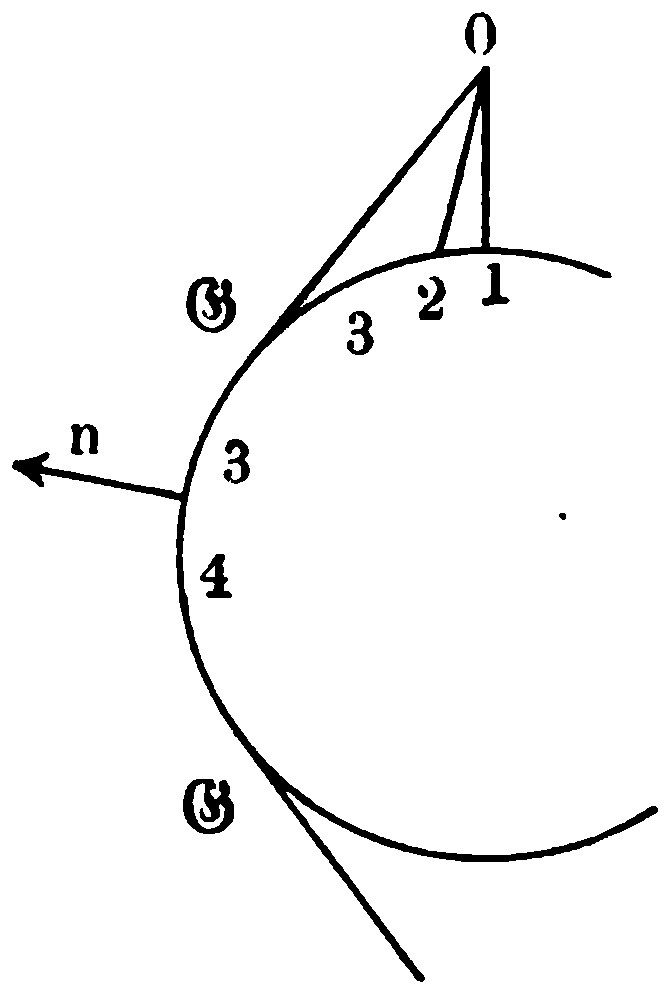
\includegraphics[width=.36\linewidth,height=48mm,keepaspectratio]{figures/fig22_accepted_derivative.png}
\end{center}
一条极值曲线（图~22）在点1处与边界相交；在该极值曲线上，点0与点1的距离如此之小，以至于弧01可以被一个场包围，该场的极值曲线经过点0。这个场也包含边界上靠近点1的部分，例如直到点2，而折线012是将要研究极值出现情况的组合曲线的一部分。那么，对于属于该场的边界弧段，可以使用在\S~20中为曲线$\Omega$所证明的一切内容；如果 $x$ 和 $y$ 沿边界都是 \S~17 意义下的函数 $\varphi(\tau)$，则 $\tau$ 沿方向 12 增长，且点 3 沿边界连续经过位置 1 时，有

\[
\frac{d(\overline{J}_{03}+\overline{J}_{32})}{d\tau}
=\mathfrak{E}\left(x,y,x',y',\frac{dx}{d\tau},\frac{dy}{d\tau}\right)\bigg|^3,
\]
其中量 $x'$、$y'$ 指沿从 0 到 1 的方向遍历的极值曲线 01。因此，若量 $\mathfrak{E}$ 不为零，则即使点 1 与点 3 的距离任意小，和 $\overline{J}_{03}+\overline{J}_{32}$ 仍既可大于、也可小于 $\overline{J}_{01}+J_{12}$；所以后一个量必定不是积分 $J$ 的极值。若该极值应由折线 012 给出，则必有方程

\[
\mathfrak{E}\left(x,y,x',y',\frac{dx}{d\tau},\frac{dy}{d\tau}\right)\bigg|^1=0
\]
成立，即要么极值曲线与边界相切，并且使得前进方向 012 在

% src-pdfpage=0199
点 1 连续地变化，或者量 $\mathfrak{E}$ 必须异常地消失。

极值的另一个必要条件是通过将属于所求曲线的边界段34进行变分而得到的，变分时应保持端点固定，并且坐标的变分具有与\S~2中相同的性质。然后设

\[
\frac{F_x-F'_{x'}}{y'}=-\frac{F_y-F'_{y'}}{x'}=M,
\]
由此得出

\[
\delta J=\int M(y'\delta x-x'\delta y)\,dt,
\]
\[
\Delta J=\delta J+\int[\delta x,\delta y,\delta x',\delta y']_2\,dt.
\]
这里，每一点 $(x+\delta x,y+\delta y)$ 都必须属于所求曲线受其约束的区域 $\mathfrak{G}$。以 $n$ 表示边界指向区域 $\mathfrak{G}$ 内部的法线，以 $\varepsilon$ 表示正常数，则下列假设满足上述要求：

\[
\delta x=\varepsilon\cos(nx)(t-t_3)^3(t_4-t)^3,
\]
\[
\delta y=\varepsilon\cos(ny)(t-t_3)^3(t_4-t)^3,
\]
并且人们得到

\[
\delta J=\varepsilon\int_3^4 [y'\cos(nx)-x'\cos(ny)]M(t-t_3)^3(t_4-t)^3\,dt,
\]
\[
\Delta J=\delta J+[\varepsilon]_2.
\]
因此，若 $\Delta J$ 具有固定的符号，则当积分 $\delta J:\varepsilon$ 不消失时，它也必须具有该符号；由于点 3 和点 4 可以任意接近，因此量

\[
[y'\cos(nx)-x'\cos(ny)]M,
\]
如果不消失，就必须具有由 $\Delta J$ 所要求的符号，即在最大值情况下为负，在最小值情况下为正。现在这个行列式

\[
\begin{vmatrix}
\cos(nx)&\cos(ny)\\
dx&dy
\end{vmatrix}
\]
为正或负，取决于方向 $n$ 相对于元素 $(dx,dy)$ 的方向，即积分方向，其取向关系或与下述关系相同，或与之

% src-pdfpage=0200
相反：即相对于 $+x$ 轴到 $+y$ 轴的取向；等价地，取决于积分时按负向还是正向绕区域 $\mathfrak{G}$ 行进。在第一种情况下，若要出现极大值，则

\[
M\leqq 0,
\]
当寻求最小值时，

\[
M\geqq 0;
\]
在第二种情况下，这些不等式会交换它们的意义。

\textbf{第一个例子。} 在平面两点之间作一条不越出给定区域 $\mathfrak{G}$ 边界的最短线。

只有当连接这两个点的直线段与边界相交时，这个问题才有意义，此时这条直线段不再是所求的最短连接，必须考虑由直线段和边界部分组成的组合。现在

\[
F=\sqrt{x'^2+y'^2},\quad
M=\frac{1}{x'}\frac{d}{dt}\left(\frac{y'}{\sqrt{x'^2+y'^2}}\right),
\]
因此，$\mathfrak{E}$ 不会异常消失；这些直线段在与边界相接处必须同边界相切。再以 $ds$ 表示沿积分方向的一个边界线元，则有

\[
M=\frac{1}{x'}\frac{d\cos(ds,y)}{dt}.
\]
因此，若 $x'>0$，坐标轴按通常方式定向，并出现上述第一种情形，即区域 $\mathfrak{G}$ 位于沿 $ds$ 方向前进者的右侧，那么为使极小值成为可能，$\cos(ds,y)$ 必须增大，也就是说，角 $(ds,y)$ 减小，$ds$ 按正向向左转动；边界的凹侧也位于同一侧。因此，凡边界构成一条最短连接的一部分时，它必向所围区域内部凸出。图形的其他可能定向也给出同样结论。

同样，对于一个其线元用等距坐标表示的曲面，也可以很容易地通过在 \S~34 中使用的测地曲率表达式，得出
% END PHYSICALLY EMBEDDED BODY INH04 5/5
\endgroup
\KneserUnitEnd{INH04}
\clearpage
\KneserUnitStart{INH05}
\begingroup
\KneserInheritedLayout\KneserTagsLeft\KneserReportTagSide{INH05}
\setcounter{equation}{0}
% BEGIN PHYSICALLY EMBEDDED BODY INH05 1/1: inherited/INH05_pdf201_248_producer_r1/tex/INH05_ZH_HANS_BODY.tex
% src-pdfpage=0201
一条界线，凡在它属于一条最短连线之处，都必须使其测地凸的一侧朝向所围区域的内部，也就是说，界线的曲率半径在曲面切平面上的投影指向该区域的外侧。

\textbf{第二个例子。} 对于问题 II（\S~9），显然适宜只在区域 $y\geqq 0$ 中寻找所求曲线，并把旋转轴 $y=0$ 看作界线；一般而言，极值曲线并不穿过后者。然而，由于令
\[
F=y\sqrt{x'^2+y'^2},
\]
极值曲线方程
\[
F_x-\frac{d}{dt}\frac{yx'}{\sqrt{x'^2+y'^2}}=0,
\quad
F_y-F'_{y'}=\sqrt{x'^2+y'^2}-\frac{d}{dt}\left(\frac{yy'}{\sqrt{x'^2+y'^2}}\right)=0
\]
在取
\[
x'=0
\]
时也得到满足，因而直线 $x=\mathrm{const.}$ 也应视为极值曲线。在 $y$ 轴上，量 $\mathfrak{E}$ 对于确定它的弧元素的任意方向都消失；而且由于它含因子 $y$，这种消失是反常的；此外，当 $y=0$, $x'>0$ 时有方程
\begin{equation}\tag{5}
M=-\frac{1}{x'}(F_y-F'_{y'})=-1.
\end{equation}
现在若沿 $x$ 轴朝 $x$ 增大的方向积分，区域 $\mathfrak{G}$ 便按正向被环绕，于是所区分的第二种情形出现；关于 $M$ 的极小条件因而得到满足。因此，可以把如下折线看作该问题的一个不连续解：它由旋转轴的一段以及在其两个端点处竖立的、长度任意的正向纵坐标线段组成；也就是说，对这条折线路径而言，这里所考察的极小值必要条件均得到满足。

\begin{center}
{\small 图 23.}\par\vspace{1mm}
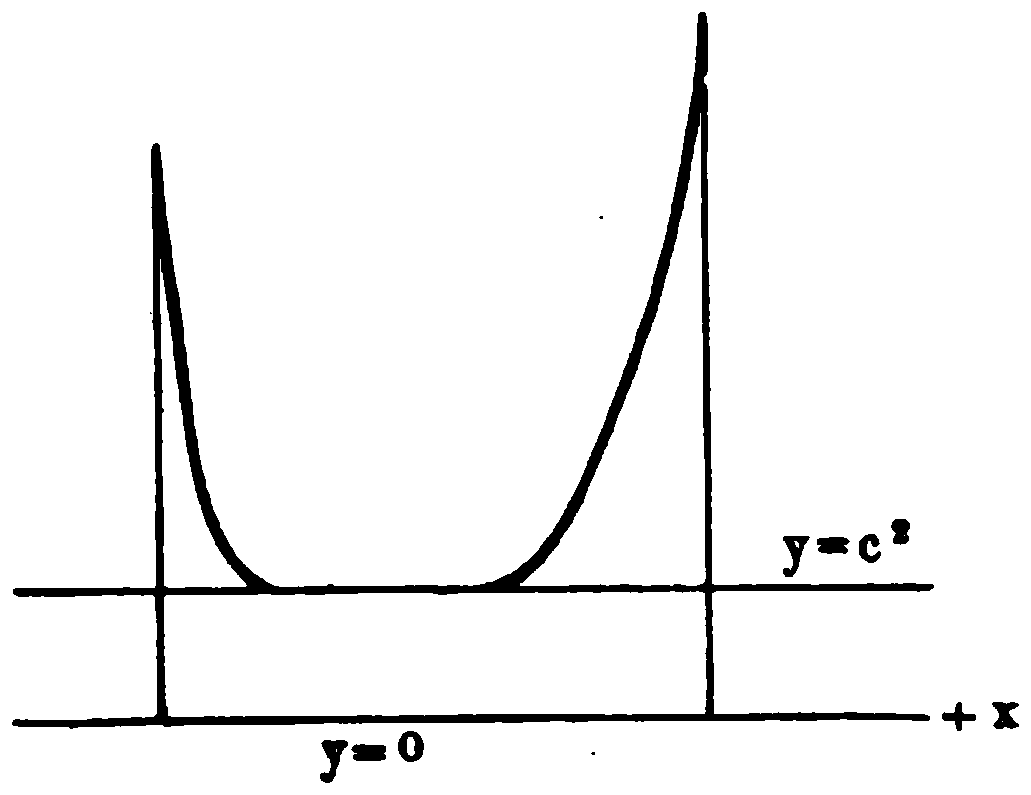
\includegraphics[width=.48\linewidth,height=42mm,keepaspectratio]{figures/fig23_accepted_derivative.png}
\end{center}

半平面 $y>0$ 中的两点总能由一条具有上述性质的折线连接，
% src-pdfpage=0202
但绝非总能由一段极值曲线连接；由此可见，引入折线有助于求解这一极值问题。

若引入直线 $y=c^2$ 作为界线（图~23，第~179~页），并且对于给定两点 $y-c^2$ 为正，则沿 $x$ 增大方向走过的界线满足方程 (5)，而量 $\mathfrak{E}$ 只能以正常方式消失。因此，所求线必须由直线 $y=c^2$ 的若干段以及与之相切且不退化为直线 $x=\mathrm{const.}$ 的悬链线弧组成。

\begin{center}
{\large \S~45.}
\end{center}

与第四篇中一样，设积分
\[
J=\int Fdt
\]
在积分
\[
K=\int Gdt
\]
取给定值的条件下达到极值。沿着通过点 1 的一条极值曲线 $\mathfrak{C}$，设在该点邻域中 $y$ 可表示为 $x$ 的正则函数，并且量
\[
F_{y'y'}+\lambda G_{y'y'}=x'^2H_1
\]
不为零；于是根据 \S~27，点 1 与曲线 $\mathfrak{C}$ 邻域中的全部极值曲线可表为
\[
y=\Phi(x,a,b,\lambda)
\]
且函数 $\Phi$ 在由曲线 $\mathfrak{C}$ 所确定的值系 $(x_1,a^0,b^0,\lambda^0)$ 邻域内是正则的。特别地，我们考察所有通过 1 并且还通过曲线 $\mathfrak{C}$ 上一点 0 的极值曲线；于是，方程
\begin{equation}\tag{6}
y_1=\Phi(x_1,a,b,\lambda),\quad y_0=\Phi(x_0,a,b,\lambda)
\end{equation}
会把量 $a$ 和 $b$ 确定为 $\lambda$ 的函数，只要行列式
\[
\Psi(x_0,x_1,a^0,b^0,\lambda^0)=
\begin{vmatrix}
\Phi_a(x_1,a^0,b^0,\lambda^0)&\Phi_b(x_1,a^0,b^0,\lambda^0)\\
\Phi_a(x_0,a^0,b^0,\lambda^0)&\Phi_b(x_0,a^0,b^0,\lambda^0)
\end{vmatrix}
\]
% src-pdfpage=0203
不为零。由于显然可以令
\[
\Phi(x,a,b,\lambda)=y_1+a+b(x-x_1)+[x-x_1]_2,
\]
所以得到
\[
\Phi_a(x,a,b,\lambda)=1+[x-x_1]_2,
\quad
\Phi_b(x,a,b,\lambda)=x-x_1+[x-x_1]_2;
\]
上述行列式因而具有形式
\[
\begin{vmatrix}
1&0\\
1+[x_0-x_1]_2&x_0-x_1+[x_0-x_1]_2
\end{vmatrix},
\]
而只要量 $|x_1-x_0|$ 充分小，它就不为零。此时，方程 (6) 给出
\[
0=\Phi_a(x_1,a,b,\lambda)\frac{da}{d\lambda}
+\Phi_b(x_1,a,b,\lambda)\frac{db}{d\lambda}
+\Phi_\lambda(x_1,a,b,\lambda),
\]
\[
0=\Phi_a(x_0,a,b,\lambda)\frac{da}{d\lambda}
+\Phi_b(x_0,a,b,\lambda)\frac{db}{d\lambda}
+\Phi_\lambda(x_0,a,b,\lambda),
\]
此外，显然还须把 $\overline{K}_{01}$ 看成 $\lambda$ 的一个函数；对它有方程
\[
\frac{d\overline{K}_{01}}{d\lambda}
=\frac{\partial\overline{K}_{01}}{\partial a}\frac{da}{d\lambda}
+\frac{\partial\overline{K}_{01}}{\partial b}\frac{db}{d\lambda}
+\frac{\partial\overline{K}_{01}}{\partial\lambda}
\]
成立，其中各偏导数是在 $x_0$ 和 $x_1$ 保持不变、而 $y_0$ 和 $y_1$ 不保持不变的假定下形成的。由此得到
\[
0=\begin{vmatrix}
\Phi_a(x_0,a,b,\lambda)&\Phi_b(x_0,a,b,\lambda)&\Phi_\lambda(x_0,a,b,\lambda)\\
\Phi_a(x_1,a,b,\lambda)&\Phi_b(x_1,a,b,\lambda)&\Phi_\lambda(x_1,a,b,\lambda)\\
\dfrac{\partial\overline{K}_{01}}{\partial a}&\dfrac{\partial\overline{K}_{01}}{\partial b}&\dfrac{\partial\overline{K}_{01}}{\partial\lambda}-\dfrac{d\overline{K}_{01}}{d\lambda}
\end{vmatrix}
\]
或
\[
\Delta(x_0,x_1)=\frac{d\overline{K}_{01}}{d\lambda}\cdot\Psi(x_0,x_1,a,b,\lambda).
\]
根据 \S~42，只要点 0 与点 1 的距离充分小，并且令
\begin{equation}\tag{7}
a=a^0,\quad b=b^0,\quad \lambda=\lambda^0
\end{equation}
上述方程的左边就不为零；此时量 $\Psi$ 有限，故得到
\begin{equation}\tag{8}
0\gtrless \frac{d\overline{K}_{01}}{d\lambda}\bigg|^{a=a^0,\,b=b^0,\,\lambda=\lambda^0}.
\end{equation}
现在显然有
% src-pdfpage=0204
\[
\begin{aligned}
\frac{d\overline{K}_{01}}{d\lambda}
&=\frac{d}{d\lambda}\int_{x_0}^{x_1}g(x,y,p)\,dx \\
&=\int_{x_0}^{x_1}\left\{g_y\left(\Phi_a\frac{da}{d\lambda}+\Phi_b\frac{db}{d\lambda}+\Phi_\lambda\right)\right.\\
&\hspace{18mm}\left.+g_p\frac{d}{dx}\left(\Phi_a\frac{da}{d\lambda}+\Phi_b\frac{db}{d\lambda}+\Phi_\lambda\right)\right\}\,dx \\
&=g_p\left(\Phi_a\frac{da}{d\lambda}+\Phi_b\frac{db}{d\lambda}+\Phi_\lambda\right)\bigg|_{x_0}^{x_1}\\
&\hspace{10mm}+\int_{x_0}^{x_1}\left(g_y-\frac{dg_p}{dx}\right)
\left(\Phi_a\frac{da}{d\lambda}+\Phi_b\frac{db}{d\lambda}+\Phi_\lambda\right)\,dx \\
&=\int_{x_0}^{x_1}\left(g_y-\frac{dg_p}{dx}\right)
\left(\Phi_a\frac{da}{d\lambda}+\Phi_b\frac{db}{d\lambda}+\Phi_\lambda\right)\,dx.
\end{aligned}
\]
并且同样有
\[
\frac{d\overline{J}_{01}}{d\lambda}
=\int_{x_0}^{x_1}\left(f_y-\frac{df_p}{dx}\right)
\left(\Phi_a\frac{da}{d\lambda}+\Phi_b\frac{db}{d\lambda}+\Phi_\lambda\right)\,dx;
\]
又因每条极值曲线都满足方程
\[
f_y-\frac{df_p}{dx}+\lambda\left(g_y-\frac{dg_p}{dx}\right)=0
\]
所以得到
\begin{equation}\tag{9}
-\frac{d\overline{J}_{01}}{d\lambda}=\lambda\frac{d\overline{K}_{01}}{d\lambda},
\end{equation}
而由于我们假定 $\lambda$ 不为零，在假定 (7) 下，此方程的左边也不为零。这里显然有展开式
\[
\overline{J}_{01}(\lambda)=\overline{J}_{01}(\lambda^0)+(\lambda-\lambda^0)\left(\frac{d\overline{J}_{01}}{d\lambda}\right)_{\lambda=\lambda^0}+[\lambda-\lambda^0]_2,
\]
\[
\overline{K}_{01}(\lambda)=\overline{K}_{01}(\lambda^0)+(\lambda-\lambda^0)\left(\frac{d\overline{K}_{01}}{d\lambda}\right)_{\lambda=\lambda^0}+[\lambda-\lambda^0]_2.
\]
现在对第二条极值曲线 $\mathfrak{C}_1$ 重复上述全部考察，点 2 和点 3 位于该曲线上；属于它的 $\lambda$ 值用 $\lambda_+^0$ 表示，为对称起见，在先前各式中用 $\lambda_-$ 代替 $\lambda$；一般地，用所附的符号 $-$、$+$ 表明某个量应分别与曲线 $\mathfrak{C}$ 或 $\mathfrak{C}_1$ 有关；于是得到方程
% src-pdfpage=0205
\[
\overline{J}_{23}(\lambda_+)=\overline{J}_{23}(\lambda_+^0)+
(\lambda_+-\lambda_+^0)\left(\frac{d\overline{J}_{23}}{d\lambda_+}\right)_{\lambda_+=\lambda_+^0}
+[\lambda_+-\lambda_+^0]_2,
\]
\[
\overline{K}_{23}(\lambda_+)=\overline{K}_{23}(\lambda_+^0)+
(\lambda_+-\lambda_+^0)\left(\frac{d\overline{K}_{23}}{d\lambda_+}\right)_{\lambda_+=\lambda_+^0}
+[\lambda_+-\lambda_+^0]_2.
\]
现在假定曲线 $\mathfrak{C}$ 和 $\mathfrak{C}_1$ 是某条以任意方式拼合而成的线路的组成部分；该线路虽不具备 \S~2 所考察曲线 $\mathfrak{B}$ 的连续性性质，却使积分 $J$ 在 $K$ 取给定值时达到极值。于是作如下变分：用端点相同的另一些极值曲线弧替换曲线 $\mathfrak{C}_1$ 和 $\mathfrak{C}$ 的弧 23 与 01，并沿用上述记号。由于沿变分后线路的积分 $K$ 应与沿原线路的值相同，故有
\[
\overline{K}_{01}(\lambda_-)+\overline{K}_{23}(\lambda_+)
=\overline{K}_{01}(\lambda_-^0)+\overline{K}_{23}(\lambda_+^0),
\]
因此量 $\lambda_-$、$\lambda_+$ 由下列关系联系：
\[
0=(\lambda_- -\lambda_-^0)\left(\frac{d\overline{K}_{01}}{d\lambda_-}\right)_{\lambda_- =\lambda_-^0}
+(\lambda_+ -\lambda_+^0)\left(\frac{d\overline{K}_{23}}{d\lambda_+}\right)_{\lambda_+ =\lambda_+^0}
+[\lambda_- -\lambda_-^0,\lambda_+ -\lambda_+^0]_2.
\]
极值要求量
\[
\overline{J}_{01}(\lambda_-)+\overline{J}_{23}(\lambda_+)-\overline{J}_{01}(\lambda_-^0)-\overline{J}_{23}(\lambda_+^0)
\]
具有固定符号。由于它可以表为
\[
(\lambda_- -\lambda_-^0)\left(\frac{d\overline{J}_{01}}{d\lambda_-}\right)_{\lambda_- =\lambda_-^0}
+(\lambda_+ -\lambda_+^0)\left(\frac{d\overline{J}_{23}}{d\lambda_+}\right)_{\lambda_+ =\lambda_+^0}
\]
\[
+[\lambda_+ -\lambda_+^0,\lambda_- -\lambda_-^0]_2
\]
故由 \S~7 的一般定理得到
\[
0=
\begin{vmatrix}
\dfrac{d\overline{J}_{01}}{d\lambda_-}&\dfrac{d\overline{J}_{23}}{d\lambda_+}\\[1.2ex]
\dfrac{d\overline{K}_{01}}{d\lambda_-}&\dfrac{d\overline{K}_{23}}{d\lambda_+}
\end{vmatrix}
\]
其中 $\lambda_- =\lambda_-^0$, $\lambda_+ =\lambda_+^0$。由此并利用关系 (8)、(9) 以及关于曲线 23 的相应关系，得到
\[
0=\frac{d\overline{K}_{01}}{d\lambda_-}\frac{d\overline{K}_{23}}{d\lambda_+}
\begin{vmatrix}
\lambda_-^0&\lambda_+^0\\
1&1
\end{vmatrix},
\quad \lambda_-^0=\lambda_+^0.
\]
% src-pdfpage=0206
此方程表达了 \textsc{Mayer} 所提出的等周常数守恒定律的最简单情形；根据所得结果，该常数对于 $\mathfrak{C}$ 和 $\mathfrak{C}_1$ 具有同一数值。

\textbf{例。} 在点 0 和点 2 之间作一条长度给定的线，使其通过给定点 1，并与直线段 02 围成尽可能大的面积。

若所求曲线在 0 与 1 之间以及 1 与 2 之间都没有不连续性，则弧 01 与 12 必须是极值曲线，因而必为圆；这是根据 \S~43 中得出相应结果的论证。依照刚刚得到的定理，所求线必由两段半径相同的圆弧 01、12 组成。让该半径变化，容易看出，两弧的总长度在一定界限内可以取任意值。

% machine-unit: Kneser_LVR_DE_p0206_p0219 §§46-48
% src-pdfpage=0206
% src-break=0206
\begin{center}
{\large \S~46.}
\end{center}

现在设极值曲线 $\mathfrak{C}$ 和 $\mathfrak{C}_1$ 共有点 1；取点 0 和 2 充分接近点 1，使得通过前者的极值曲线围绕弧 01 的每一部分形成一个场，而通过后者的极值曲线围绕弧 12 的每一部分形成一个场；若 $H_1$ 沿弧 01 和 12 不消失，根据 \S~41 这是可能的（图~21，第~172~页）。将两个场表示为方程组
\[
 x=\xi_-(t_-,a_-,b_-),\quad y=\eta_-(t_-,a_-,b_-),
\]
\[
 x=\xi_+(t_+,a_+,b_+),\quad y=\eta_+(t_+,a_+,b_+)
\]
则每个与点 1 充分接近的点 3 都可以通过这些场中的极值曲线分别同 0 和 2 连接。把点 3 看作可在位置 1 附近变动，便得到（\S~35）
\begin{equation}\tag{10}
\frac{\partial\overline K_{03}}{\partial t_-}=G_-\bigg|^3,
\quad
\frac{\partial\overline K_{03}}{\partial a_-}
=\int_0^3\bigl[\xi_a(G_x-G_{x'}')+\eta_a(G_y-G_{y'}')\bigr]_-\,dt_-
+\bigl(\xi_aG_{x'}+\eta_aG_{y'}\bigr)_-\bigg|^3
\end{equation}
以及一个把 $a$ 换成 $b$ 的类似公式；因此，若从点 1 到点 3 以及从弧 01 到弧 03 的过渡分别对应增量 $\delta t_-$、$\delta a_-$、$\delta b_-$，则
% src-pdfpage=0207
\[
\overline K_{03}-\overline K_{01}=\Delta\overline K_{01}
=G_{x'}^-\delta x+G_{y'}^-\delta y\bigg|^1
+A_-\delta a_-+B_-\delta b_-+[\delta t_-,\delta a_-,\delta b_-]_2,
\]
其中令
\begin{equation}\tag{11}
\delta x=(\xi_a\delta a+\xi_b\delta b+\xi_t\delta t)_-,
\quad
\delta y=(\eta_a\delta a+\eta_b\delta b+\eta_t\delta t)_-,
\end{equation}
\[
A_- =\int_0^1\bigl[\xi_a(G_x-G_{x'}')+\eta_a(G_y-G_{y'}')\bigr]_-\,dt_-
\]
而 $B_-$ 由 $A_-$ 中把 $a$ 换成 $b$ 得到。类似地得到
\[
\Delta\overline K_{12}
=-G_{x'}^+\delta x-G_{y'}^+\delta y\bigg|^1
+A_+\delta a_+ +B_+\delta b_+ +[\delta t_+,\delta a_+,\delta b_+]_2,
\]
其中量 $\delta t_+$、$\delta a_+$、$\delta b_+$、$A_+$、$\ldots$ 对极值曲线 12 所具有的意义，与 $\delta t_-$、$\ldots$ 对 01 所具有的意义相类似，因而
\begin{equation}\tag{12}
\delta x=(\xi_a\delta a+\xi_b\delta b+\xi_t\delta t)_+,
\quad
\delta y=(\eta_a\delta a+\eta_b\delta b+\eta_t\delta t)_+.
\end{equation}
现在，若 $J$ 要在 $K$ 取给定值时达到极值，则只要把八个量 $\delta x$、$\delta y$、$\delta a_\pm$、$\delta b_\pm$、$\delta t_\pm$ 确定得使方程
\[
\Delta\overline K_{01}+\Delta\overline K_{12}=0
\]
成立，便可用由极值曲线弧 03、32 构成的折线作为折线 012 的容许变分；换言之，须有
\begin{equation}\tag{13}
\begin{aligned}
0={}&(G_{x'}^- -G_{x'}^+)\delta x+(G_{y'}^- -G_{y'}^+)\delta y\bigg|^1 \\
&+A_-\delta a_-+B_-\delta b_-+A_+\delta a_+ +B_+\delta b_+ \\
&+[\delta a_+,\delta b_+,\delta t_+,\delta a_-,\delta b_-,\delta t_-]_2.
\end{aligned}
\end{equation}
此方程连同 (11) 和 (12) 中所列方程，可以用来把八个量 $\delta$ 中的五个表示为其余三个的函数。例如若取后者为 $\delta x$、$\delta y$、$\delta a_+$，则上述五个方程右边关于量 $\delta t_-$、$\delta a_-$、$\delta b_-$、$\delta t_+$、$\delta b_+$ 的线性项所成的行列式为
% src-pdfpage=0208
\begin{equation}\tag{14}
\begin{vmatrix}
0&A_-&B_-&0&B_+\\
\xi_t^-&\xi_a^-&\xi_b^-&0&0\\
\eta_t^-&\eta_a^-&\eta_b^-&0&0\\
0&0&0&\xi_t^+&\xi_b^+\\
0&0&0&\eta_t^+&\eta_b^+
\end{vmatrix}
=
\begin{vmatrix}
0&A_-&B_-\\
\xi_t^-&\xi_a^-&\xi_b^-\\
\eta_t^-&\eta_a^-&\eta_b^-
\end{vmatrix}
\left[\frac{\partial(\xi,\eta)}{\partial(t,b)}\right]_+ .
\end{equation}
在右边第一个行列式中，把第二、第三横行分别乘以 $G_{x'}^-$ 和 $G_{y'}^-$ 后加到第一行上，并注意到 $\xi$ 和 $\eta$ 的导数如方程 (11) 中那样是就点 1 而言的，方程 (10) 就表明该行列式具有数值
\[
\frac{\partial(\overline K_{01},\xi_-,\eta_-)}{\partial(t_-,a_-,b_-)}
\]
也就是说，它等于与弧 01 的场有关的量 $\Delta_-$，因而不为零。此外，弧 12 也被一个场所围绕，而对于该场，量
\[
\frac{\partial(\xi_+,\eta_+,\overline K_{21})}{\partial(t_+,a_+,b_+)}
\]
不消失，所以根据 \S~35，量
\[
\left[\frac{\partial(\xi,\eta)}{\partial(t,a)}\right]_+,
\quad
\left[\frac{\partial(\xi,\eta)}{\partial(t,b)}\right]_+
\]
不同时为零；因而，或者方程 (14) 右边的第二个因子也不为零，或者交换 $a_+$ 与 $b_+$ 后即可做到这一点。因此，总能把五个量 $\delta$ 表示为其余三个量的幂级数，而在这三个量中包含 $\delta x$ 和 $\delta y$。

现在若在表达式 $A$、$B$ 中把函数符号 $G$ 换成 $F$，所得量记为 $\mathfrak A$、$\mathfrak B$；于是极值曲线方程给出
\begin{equation}\tag{15}
\lambda_-A_-+\mathfrak A_-=
\lambda_-B_-+\mathfrak B_-=
\lambda_+A_+ +\mathfrak A_+=
\lambda_+B_+ +\mathfrak B_+=0,
\end{equation}
并且根据上一节，对于 $\mathfrak C$ 和 $\mathfrak C_1$ 有
\[
\lambda_+=\lambda_-=\lambda.
\]
此外，与方程 (13) 中展开的表达式 $\Delta\overline K_{01}+\Delta\overline K_{12}$ 类似，可得
% src-pdfpage=0209
\[
\begin{aligned}
\Delta\overline J_{01}+\Delta\overline J_{12}
={}&(F_{x'}^- -F_{x'}^+)\delta x+(F_{y'}^- -F_{y'}^+)\delta y\bigg|^1\\
&+\mathfrak A_-\delta a_-+\mathfrak B_-\delta b_-+\mathfrak A_+\delta a_+ +\mathfrak B_+\delta b_+ \\
&+[\delta a_\pm,\delta b_\pm,\delta t_\pm]_2;
\end{aligned}
\]
因此，把方程 (13) 乘以 $\lambda$ 并加到最后一式上，因 $H=F+\lambda G$，由 (15) 得到
\[
\Delta\overline J_{01}+\Delta\overline J_{12}
=(H_{x'}^- -H_{x'}^+)\delta x+(H_{y'}^- -H_{y'}^+)\delta y\bigg|^1
+[\delta a_\pm,\delta b_\pm,\delta t_\pm]_2.
\]
当所要求的极值存在时，这个量在条件 (11)、(12)、(13) 下必须具有固定符号；由于线性项中只出现量 $\delta x$、$\delta y$，根据 \S~7，在点 1 处得到
\begin{equation}\tag{16}
(H_{x'}^- -H_{x'}^+)\delta x+(H_{y'}^- -H_{y'}^+)\delta y=0.
\end{equation}
因此，按照点 1 是可以自由移动，还是受限于曲线
\[
h(x,y)=0
\]
分别得到关系
\[
H_{x'}^- -H_{x'}^+=H_{y'}^- -H_{y'}^+=0
\]
或
\[
\begin{vmatrix}
H_{x'}^- -H_{x'}^+&H_{y'}^- -H_{y'}^+\\
h_x&h_y
\end{vmatrix}=0.
\]
所以，对于一个角点，所得限制恰好与 \S~43 中绝对极值情形下的限制相同，只须把 $F$ 换成 $F+\lambda G$。

\textbf{例。问题 IX}（\S~34）。有
\[
H=yx' +\lambda\sqrt{x'^2+y'^2},
\]
\[
H_{x'}=y+\frac{\lambda x'}{\sqrt{x'^2+y'^2}},
\quad
H_{y'}=\frac{\lambda y'}{\sqrt{x'^2+y'^2}};
\]
所以方程 (16) 给出
\begin{equation}\tag{17}
\lambda\left(\frac{x'\delta x+y'\delta y}{\sqrt{x'^2+y'^2}}\right)_-
=
\lambda\left(\frac{x'\delta x+y'\delta y}{\sqrt{x'^2+y'^2}}\right)_+.
\end{equation}
由于 $\lambda$ 不为零，对于一个可自由处置的角点便会得到
\[
\left(\frac{x'}{\sqrt{x'^2+y'^2}}\right)_-
=
\left(\frac{x'}{\sqrt{x'^2+y'^2}}\right)_+,
\quad
\left(\frac{y'}{\sqrt{x'^2+y'^2}}\right)_-
=
\left(\frac{y'}{\sqrt{x'^2+y'^2}}\right)_+,
\]
% src-pdfpage=0210
也就是说，极值曲线 01 与 12 在点 1 处的方向必然一致，因而不会发生不连续。反之，若点 1 被约束在曲线 $\mathfrak K$ 上，该曲线的弧元素为 $Ds$；并且在点 1 处以 $-$、$+$ 分别表示极值曲线 01 从 0 朝向 1 的方向以及极值曲线 12 从 1 朝向 2 的方向，则由方程 (17) 得到
\[
\cos(Ds,-)=\cos(Ds,+).
\]
因此，弧 01 与 12 位于曲线 $\mathfrak K$ 的同一侧，并同其切线构成大小相等、向不同方向张开的锐角，也就是说，它们的位置如入射光线和反射光线一般。

例如，若要从给定点 5 出发，向曲线 $\mathfrak K$ 上一个未预先指定的点 1 作线，再返回点 5，从而构成一条长度给定且围成面积尽可能大的闭合线，那么它必须由两段半径相同的圆弧组成，并且按上述意义同曲线 $\mathfrak K$ 构成相等的角。

\begin{center}
{\large \S~47.}
\end{center}

还须考察在求解等周问题时，何种情况下会出现线路 0123：所比较的曲线限于由界线围成的区域 $\mathfrak G$ 内，线段 12 属于一条界线，而弧 01 和 23 不属于界线，因而根据 \S~45，后二者是具有同一等周常数的极值曲线。此时（图~24）取点 0 和 3 分别充分接近点 1 和 2，使弧 01 和 23 可被其极值曲线通过 0 和 3 的场所围绕。在界线上的点 1 和 2 附近取点 4 和 5；于是存在属于这两个场的极值曲线 04 和 53。若有
\[
\overline K_{01}+K_{12}+\overline K_{23}=\overline K_{04}+K_{45}+\overline K_{53},
\]
或
\begin{equation}\tag{18}
K_{12}-K_{45}=\Delta\overline K_{01}+\Delta\overline K_{23},
\end{equation}
则线路 0453 是线路 0123 的容许变分。
\begin{center}
{\small 图 24.}\par\vspace{1mm}
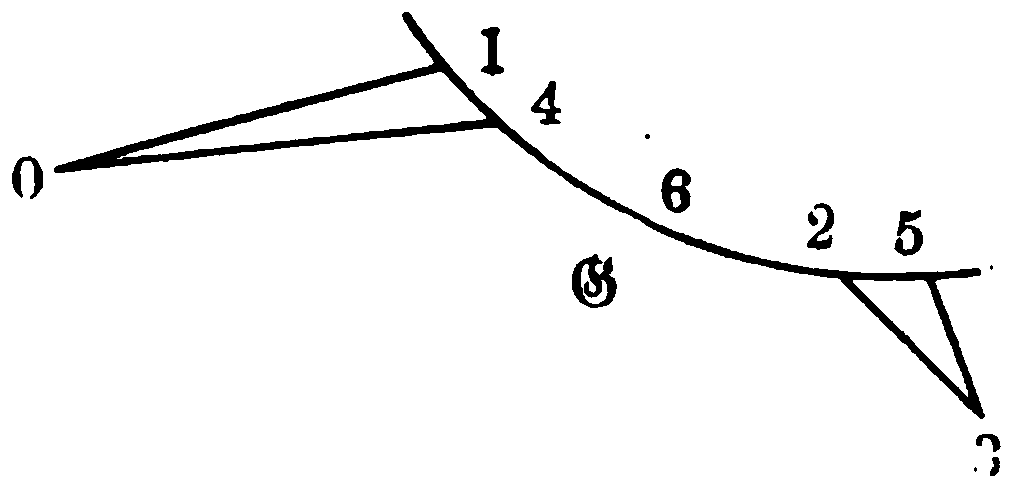
\includegraphics[width=.48\linewidth,height=42mm,keepaspectratio]{figures/fig24_accepted_derivative.png}
\end{center}
% src-pdfpage=0211
这里，无横线的积分始终指界线上的积分，而符号 $\Delta$ 表示从 01、23 过渡到 04、53 时的增量。为讨论这一要求，我们赋予符号 $\xi$、$\eta$、$t_+$、$a_\pm$、$b_\pm$、$A_\pm$、$\delta t_\pm\ldots$ 与上一节中它们对弧 01 和 12 所具有的相同意义，不过这里是对弧 01 和 23 而言；符号 $-$ 属于前一弧，符号 $+$ 属于后一弧；相应地令
\[
\begin{aligned}
\delta x_-+[\delta t_-,\delta a_-,\delta b_-]_2&=x_4-x_1,\\
\delta y_-+[\delta t_-,\delta a_-,\delta b_-]_2&=y_4-y_1,\\
\delta x_++[\delta t_+,\delta a_+,\delta b_+]_2&=x_5-x_2,\\
\delta y_++[\delta t_+,\delta a_+,\delta b_+]_2&=y_5-y_2,
\end{aligned}
\]
并且表达式 $\delta x$、$\delta y$ 对 $\delta t$、$\delta a$、$\delta b$ 是线性的。于是可由 \S~46 中为 $K_{01}$ 建立的公式求得方程 (18) 的右边；确切地说，有
\begin{equation}\tag{19}
\begin{aligned}
\Delta\overline K_{01}&=G_{x'}^-\delta x_-+G_{y'}^-\delta y_-\bigg|^1
+A_-\delta a_-+B_-\delta b_-+[\delta t_-,\delta a_-,\delta b_-]_2,\\
\Delta\overline K_{23}&=-G_{x'}^+\delta x_+ -G_{y'}^+\delta y_+\bigg|^2
+A_+\delta a_+ +B_+\delta b_+ +[\delta t_+,\delta a_+,\delta b_+]_2;
\end{aligned}
\end{equation}
并且量 $\delta$ 之间现在有四个关系
\begin{equation}\tag{20}
\delta x_\pm=(\xi_t\delta t+\xi_a\delta a+\xi_b\delta b)_\pm,
\quad
\delta y_\pm=(\eta_t\delta t+\eta_a\delta a+\eta_b\delta b)_\pm,
\end{equation}
其中两边要么都取符号 $\pm$ 的上号，要么都取下号。因此，若在这里以及方程 (18) 中把量 $\delta t_-$、$\delta a_-$、$\delta b_-$、$\delta b_+$、$\delta t_+$ 看作由其余各量 $\delta$ 所确定，那么，在所列五个方程中，含这五个量的各项所组成的行列式，与上一节方程 (11)、(12)、(13) 中的行列式完全相同。那里关于此行列式或交换 $a_+$ 与 $b_+$ 后所得行列式不为零的证明，在把那里所考察的弧 12 换成 23 后仍然有效。因此，可从五个方程 (18)、(20) 解出量 $\delta t_\pm$、$\delta a_-$、$\delta b_\pm$，只要 $K_{12}-K_{45}$ 充分小。

% src-pdfpage=0212
现在设沿界线、在点 1 和 2 的邻域内，$x$ 和 $y$ 是参数 $\tau_-$、$\tau_+$ 的正则函数；这些参数沿方向 12 增大，并且在过渡到 4 和 5 时分别获得增量 $D\tau_-$ 和 $D\tau_+$；于是
\[
\delta x_- =\frac{dx}{d\tau_-}\bigg|^1D\tau_-+[D\tau_-]_2,
\quad
\delta y_- =\frac{dy}{d\tau_-}\bigg|^1D\tau_-+[D\tau_-]_2,
\]
在点 2 处也有类似方程。再假定被积函数 $F$ 和 $G$ 在线路 0123 每一元素的邻域内都是正则的，则当 $D\tau_-$ 为正值时
\begin{equation}\tag{21}
K_{14}=G\left(x,y,\frac{dx}{d\tau_-},\frac{dy}{d\tau_-}\right)\bigg|^1D\tau_-+[D\tau_-]_2,
\end{equation}
当其为负值时
\begin{equation}\tag{22}
K_{41}=G\left(x,y,\frac{dx}{d\tau_-},\frac{dy}{d\tau_-}\right)\bigg|^1(-D\tau_-)+[D\tau_-]_2.
\end{equation}
现在若在界线上任意固定一点 6，使其位于 1 与 2 之间并处于线段 14、25 之外，那么按照 $D\tau_-$ 为正或为负，有下列两个方程之一：
\[
K_{46}-K_{16}=-K_{14},
\quad
K_{46}-K_{16}=K_{41};
\]
因而无论何种情形，根据 (21)、(22) 都有
\begin{equation}\tag{23}
\Delta K_{16}=K_{46}-K_{16}
=-G\left(x,y,\frac{dx}{d\tau_-},\frac{dy}{d\tau_-}\right)\bigg|^1D\tau_-+[D\tau_-]_2.
\end{equation}
以类似方式得到
\begin{equation}\tag{24}
\Delta K_{62}=K_{65}-K_{62}
=+G\left(x,y,\frac{dx}{d\tau_+},\frac{dy}{d\tau_+}\right)\bigg|^2D\tau_+ +[D\tau_+]_2;
\end{equation}
把这些表达式之和
\[
\Delta K_{16}+\Delta K_{62}=\Delta K_{12}=K_{45}-K_{12}
\]
代入方程 (18)，则由 (19) 得到
\begin{equation}\tag{25}
\begin{aligned}
&G\left(x,y,\frac{dx}{d\tau_-},\frac{dy}{d\tau_-}\right)\bigg|^1D\tau_-
-G\left(x,y,\frac{dx}{d\tau_+},\frac{dy}{d\tau_+}\right)\bigg|^2D\tau_+\\
&\quad=G_{x'}^-\frac{dx}{d\tau_-}+G_{y'}^-\frac{dy}{d\tau_-}\bigg|^1D\tau_-
-G_{x'}^+\frac{dx}{d\tau_+}-G_{y'}^+\frac{dy}{d\tau_+}\bigg|^2D\tau_+\\
&\qquad +A_-\delta a_-+B_-\delta b_-+A_+\delta a_+ +B_+\delta b_+
+[\delta a_\pm,\delta b_\pm,\delta t_\pm,D\tau_\pm]_2.
\end{aligned}
\end{equation}

% src-pdfpage=0213
方程 (19) 的右边分别成为 $\Delta\overline J_{01}$ 和 $\Delta\overline J_{23}$，只要把 $G$ 换成 $F$，把 $A$ 和 $B$ 换成 $\mathfrak A$ 和 $\mathfrak B$；因此，把最后一个方程乘以同时属于曲线 01 和 23 的常数 $\lambda$，并利用方程 (15)，就得到
\[
\begin{aligned}
&\Delta\overline J_{01}+\Delta\overline J_{23}
+\lambda G\left(x,y,\frac{dx}{d\tau_-},\frac{dy}{d\tau_-}\right)\bigg|^1D\tau_-\\
&\quad -\lambda G\left(x,y,\frac{dx}{d\tau_+},\frac{dy}{d\tau_+}\right)\bigg|^2D\tau_+\\
&=H_{x'}^-\frac{dx}{d\tau_-}+H_{y'}^-\frac{dy}{d\tau_-}\bigg|^1D\tau_-
-H_{x'}^+\frac{dx}{d\tau_+}-H_{y'}^+\frac{dy}{d\tau_+}\bigg|^2D\tau_+\\
&\quad +[\delta a_\pm,\delta b_\pm,\delta t_\pm,D\tau_\pm]_2.
\end{aligned}
\]
现在，积分 $J_{0123}$ 在所考察的变分下取得增量
\[
\Delta\overline J_{01}+\Delta\overline J_{23}+J_{45}-J_{12}
=\Delta\overline J_{01}+\Delta\overline J_{23}+\Delta J_{16}+\Delta J_{62};
\]
又由于类似方程 (23)、(24)，可令
\[
\Delta J_{16}=-F\left(x,y,\frac{dx}{d\tau_-},\frac{dy}{d\tau_-}\right)\bigg|^1D\tau_-+[D\tau_-]_2,
\]
\[
\Delta J_{62}=F\left(x,y,\frac{dx}{d\tau_+},\frac{dy}{d\tau_+}\right)\bigg|^2D\tau_+ +[D\tau_+]_2,
\]
故该增量可表示为
\[
\begin{aligned}
&H_{x'}^-\frac{dx}{d\tau_-}+H_{y'}^-\frac{dy}{d\tau_-}
-H\left(x,y,\frac{dx}{d\tau_-},\frac{dy}{d\tau_-}\right)\bigg|^1D\tau_-\\
&\quad -H_{x'}^+\frac{dx}{d\tau_+}-H_{y'}^+\frac{dy}{d\tau_+}
+H\left(x,y,\frac{dx}{d\tau_+},\frac{dy}{d\tau_+}\right)\bigg|^2D\tau_+\\
&\quad +[\delta t_\pm,\delta a_\pm,\delta b_\pm,D\tau_\pm]_2,
\end{aligned}
\]
或简写为
\[
\Delta J_{0123}=\mathfrak E^-D\tau_- -\mathfrak E^+D\tau_+ +[\delta t_\pm,\delta a_\pm,\delta b_\pm,D\tau_\pm]_2,
\]
其中，量 $\mathfrak E^-$ 是由下列两个元素构成的：从点 1 出发、越过该点延伸的极值曲线 01 的元素，以及与 $\tau_-$ 的递增值相应的界线元素；而 $\mathfrak E^+$ 则是在点 2 处由指向点 3 的极值曲线元素以及 $\tau_+$ 增大的方向构成的。

若所求极值存在，则 $\Delta J_{0123}$ 对于所有服从关系 (20)、(25) 的量 $\delta$、$D$ 必须具有固定符号。在这些量中，$D\tau_+$ 和 $D\tau_-$ 仍可自由处置；因此 \S~7 的定理表明，
% src-pdfpage=0214
$\Delta J_{0123}$ 中不含由上述关系所确定的任何变分的线性部分，在 $D\tau_-$ 和 $D\tau_+$ 取任意值时都消失，也就是说
\[
\mathfrak E^- = \mathfrak E^+=0.
\]
因此，若排除量 $\mathfrak E$ 在点 1 和 2 处的反常消失，则在这些点处，界线必须与邻接于它的极值曲线相切；这样，这里仍得到对绝对极值已经证明的结果。

\textbf{例。问题 IX。} 量 $\mathfrak E$ 根据 \S~37 只能以正常方式消失；因此，例如若要在一个平面多边形内作一条长度给定而面积最大的闭合线，并且具有规定长度的圆无法容纳在该多边形内，那么所求线只能由多边形各边的一些部分以及与之相切、半径相同的圆弧组成。

\textbf{问题 X。} 量 $\mathfrak E$ 在 \S~34 的记号中与问题 IX 中出现的量只相差因子 $\sqrt M$，所以只要 $M$ 不为零，它就只以正常方式消失。若对于一个由正则曲线段围成的区域，这一条件成立，并要在其中作一条面积给定而长度最小的闭合线，则该线只能由围界曲线段的一些部分以及测地曲率恒定的弧组成；后面这些弧都具有同一测地曲率值，并在与界线相遇之处同它相切。这一定理由 \textsc{Steiner} 提出。

% src-pdfpage=0215
\begin{center}
{\large 第六篇。}\par
\vspace{2mm}
{\Large\bfseries 含未知函数高阶导数的\\积分的极值。}\par
\vspace{2mm}\rule{32mm}{0.4pt}\par
\vspace{2mm}
{\large \S~48.}
\end{center}

设 $\mathfrak B$ 是一段平面曲线；沿该曲线段，$x$ 和 $y$ 可表示为参数 $t$ 的连续函数，并且它们直至第 $n^{\mathrm{ten}}$ 阶（含该阶）的导数也都是 $t$ 的连续函数。函数
\[
F(x,x',x'',\ldots x^{(n)},y,y',y'',\ldots y^{(n)})
\]
对于由弧 $\mathfrak B$ 的任一元素所确定的其诸自变量值系都是正则的，并且在弧的每一点，量 $x'$、$y'$ 中至少有一个不为零。我们只考察这样的积分
\[
J=\int Fdt,
\]
其值仅由曲线 $\mathfrak B$ 决定，而不依赖于 $x$、$y$ 与 $t$ 之间联系的特殊性质。若此时 $x$ 和 $y$ 沿弧 $\mathfrak B$ 是参数 $\theta$ 的函数，并具有与先前引入的参数 $t$ 的函数相同的性质，且 0 和 1 是弧 $\mathfrak B$ 上任意两点，则必有方程
\[
J_{01}=\int_0^1 F(x,x',\ldots,y^{(n)})\,dt
=\int_0^1 F\left(x,\frac{dx}{d\theta},\ldots,\frac{d^ny}{d\theta^n}\right)d\theta
\]
成立。变量 $t$ 和 $\theta$ 的值通过曲线上的点相互对应，所以例如可把 $\theta$ 看成 $t$ 的函数；让积分上限变化，并对与该上限
% src-pdfpage=0216
相应的 $t$ 值求微分，便得到
\[
F(x,x',\ldots y^{(n)})
=F\left(x,\frac{dx}{d\theta},\ldots,\frac{d^ny}{d\theta^n}\right)\frac{d\theta}{dt},
\]
或
\begin{equation}\tag{1}
F\left(x,\frac{dx}{dt},\ldots,\frac{d^ny}{dt^n}\right)dt
=F\left(x,\frac{dx}{d\theta},\ldots,\frac{d^ny}{d\theta^n}\right)d\theta.
\end{equation}
特别地，在 $x'$ 不消失的一点，可令 $\theta=x$，也就是说，可把 $y$ 看成 $x$ 的函数；它直至第 $n^{\mathrm{ten}}$ 阶的各导数，均可表示为 $x$、$x'$、$\ldots x^{(n)}$、$y$、$y'$、$\ldots y^{(n)}$ 的整函数除以 $x'$ 的幂，因而是 $x$ 的连续函数。由于
\[
\frac{dx}{d\theta}=1,
\quad
\frac{d^2x}{d\theta^2}=\cdots=\frac{d^nx}{d\theta^n}=0,
\]
故由方程 (1) 有
\[
F(x,x',\ldots y^{(n)})dt
=F\left(x,1,0,\ldots,0,y,\frac{dy}{dx},\ldots,\frac{d^ny}{dx^n}\right)dx
\]
或用新的记号
\[
F(x,x',\ldots y^{(n)})dt
=f\left(x,y,\frac{dy}{dx},\ldots,\frac{d^ny}{dx^n}\right)dx,
\quad J=\int fdx.
\]
弧 $\mathfrak B$ 具有上述性质的一个任意表示由方程
\begin{equation}\tag{2}
x=\varphi(\theta),\quad y=\psi(\theta)
\end{equation}
给出；令 $\theta=t+\tau$，并把 $\tau$ 理解为 $t$ 的任意函数，且该函数关于某些常数 $\varepsilon$ 是齐次线性的，便得到另一个表示。此时显然有方程
\[
x=\varphi(t+\tau),\quad y=\psi(t+\tau),
\]
以及 \textsc{Taylor} 展开式
\[
x=\varphi(t)+\varphi'(t)\tau+\cdots,
\quad x-\varphi(t)=\varphi'(t)\tau+\cdots,
\]
\[
y=\psi(t)+\psi'(t)\tau+\cdots,
\quad y-\psi(t)=\psi'(t)\tau+\cdots;
\]
由此得到
\[
\frac{d^\alpha x}{dt^\alpha}-\varphi^{(\alpha)}(t)
=\frac{d^\alpha[\varphi'(t)\tau]}{dt^\alpha}+\cdots,
\quad
\frac{d^\alpha y}{dt^\alpha}-\psi^{(\alpha)}(t)
=\frac{d^\alpha[\psi'(t)\tau]}{dt^\alpha}+\cdots,
\]
其中省略的各项对于 $\tau$ 及该量的导数至少是二次的，
% src-pdfpage=0217
因而也以同样方式含有量 $\varepsilon$。另一方面，显然有
\[
\frac{d^\alpha x}{d\theta^\alpha}=\varphi^{(\alpha)}(\theta)=\varphi^{(\alpha)}(t+\tau),
\quad
\frac{d^\alpha y}{d\theta^\alpha}=\psi^{(\alpha)}(\theta)=\psi^{(\alpha)}(t+\tau);
\]
所以方程 (1) 给出
\[
F[\varphi(t+\tau),\varphi'(t+\tau),\ldots]\left(1+\frac{d\tau}{dt}\right)
\]
\[
=F\left(\varphi(t)+\tau\varphi'(t)+[\varepsilon]_2,
\varphi'(t)+\frac{d[\tau\varphi'(t)]}{dt}+[\varepsilon]_2,
\varphi''(t)+\frac{d^2[\tau\varphi'(t)]}{dt^2}+[\varepsilon]_2,\ldots\right),
\]
即，在左边按 $\tau$ 的幂展开，在右边按诸自变量中含量 $\varepsilon$ 的部分的幂展开，并用下标 $\varphi\psi$ 表示应令
\[
x=\varphi(t),\quad x'=\varphi'(t),\ldots,
\quad y=\psi(t),\quad y'=\psi'(t),\ldots
\]
便有
\[
\left(F_{\varphi\psi}+\tau\frac{dF_{\varphi\psi}}{dt}+[\varepsilon]_2\right)\left(1+\frac{d\tau}{dt}\right)
\]
\[
=F_{\varphi\psi}+\sum_{a=0}^n\left\{\left(\frac{\partial F}{\partial x^{(a)}}\right)_{\varphi\psi}\frac{d^a[\tau\varphi'(t)]}{dt^a}
+\left(\frac{\partial F}{\partial y^{(a)}}\right)_{\varphi\psi}\frac{d^a[\tau\psi'(t)]}{dt^a}\right\}+[\varepsilon]_2.
\]
因此，只保留关于常数 $\varepsilon$ 为线性的各项，便得到
\[
\tau\frac{dF_{\varphi\psi}}{dt}+F_{\varphi\psi}\frac{d\tau}{dt}
=\frac{d(F_{\varphi\psi}\tau)}{dt}
\]
\[
=\sum_{a=0}^n\left\{\left(\frac{\partial F}{\partial x^{(a)}}\right)_{\varphi\psi}\frac{d^a[\tau\varphi'(t)]}{dt^a}
+\left(\frac{\partial F}{\partial y^{(a)}}\right)_{\varphi\psi}\frac{d^a[\tau\psi'(t)]}{dt^a}\right\},
\]
或者，现在将弧 $\mathfrak B$ 用与方程 (2) 等价的
\[
x=\varphi(t),\quad y=\psi(t)
\]
来表示，并一如既往以撇号表示对 $t$ 的微分，则
\[
(F\tau)'=\sum_{a=0}^n\left\{\frac{\partial F}{\partial x^{(a)}}(x'\tau)^{(a)}+\frac{\partial F}{\partial y^{(a)}}(y'\tau)^{(a)}\right\},
\]
最后，用不定积分号写成
\begin{equation}\tag{3}
F\tau=\int dt\sum_{a=0}^n\left\{\frac{\partial F}{\partial x^{(a)}}(x'\tau)^{(a)}+\frac{\partial F}{\partial y^{(a)}}(y'\tau)^{(a)}\right\}.
\end{equation}

% src-pdfpage=0218
我们借助恒等式
\[
\int vu^{(a)}dt=vu^{(a-1)}-v'u^{(a-2)}+v''u^{(a-3)}-\cdots
+(-1)^{a-1}v^{(a-1)}u+(-1)^a\int v^{(a)}u\,dt,
\]
来变换此方程的右边；当 $u$ 和 $v$ 是 $t$ 的任意函数时，对等式两边关于 $t$ 求微分，便可明显看出其正确性。特别令
\[
v=\frac{\partial F}{\partial x^{(a)}},\quad u=x'\tau,
\]
便得到
\[
\int\frac{\partial F}{\partial x^{(a)}}(x'\tau)^{(a)}dt
=\frac{\partial F}{\partial x^{(a)}}(x'\tau)^{(a-1)}
-\frac{d}{dt}\frac{\partial F}{\partial x^{(a)}}(x'\tau)^{(a-2)}+\cdots
\]
\[
+(-1)^a\int\frac{d^a}{dt^a}\left(\frac{\partial F}{\partial x^{(a)}}\right)x'\tau\,dt.
\]
自然，这里新出现的每一个关于 $t$ 的导数都必须存在且可积；为在必要范围内保证这一点，我们引入新的假定：$x$ 和 $y$ 直至第 $2n^{\mathrm{ten}}$ 阶（含该阶）的导数均为有限且连续的。

于是可对 $a=1,2,\ldots n$ 写出所得公式；把它们相加，则右边的量 $(x'\tau)^{(b)}$ 所带因子为
\[
\frac{\partial F}{\partial x^{(b+1)}}
-\frac{d}{dt}\frac{\partial F}{\partial x^{(b+2)}}
+\frac{d^2}{dt^2}\frac{\partial F}{\partial x^{(b+3)}}-\cdots;
\]
因此，一般地令
\[
P_m=\sum_{a=0}^{n-m}(-1)^a\frac{d^a}{dt^a}\frac{\partial F}{\partial x^{(m+a)}},
\quad
Q_m=\sum_{a=0}^{n-m}(-1)^a\frac{d^a}{dt^a}\frac{\partial F}{\partial y^{(m+a)}},
\]
\[
P_0=P,\quad Q_0=Q,
\quad P_n=\frac{\partial F}{\partial x^{(n)}},
\quad Q_n=\frac{\partial F}{\partial y^{(n)}},
\]
\begin{equation}\tag{4}
P_m=\frac{\partial F}{\partial x^{(m)}}-\frac{dP_{m+1}}{dt},
\quad
Q_m=\frac{\partial F}{\partial y^{(m)}}-\frac{dQ_{m+1}}{dt},
\end{equation}
则方程 (3) 具有下列形式：
\begin{equation}\tag{5}
0=\int(Px'+Qy')\tau\,dt
+\sum_{a=1}^n\{P_a(x'\tau)^{(a-1)}+Q_a(y'\tau)^{(a-1)}\}-F\tau.
\end{equation}
% src-pdfpage=0219
现在，积分号外的所有项都可化为量 $\tau$、$\tau'$、$\ldots$、$\tau^{(n-1)}$ 的一个线性和式，其系数与 $\tau$ 无关。例如，设 $\tau^{(k)}$ 是 $\tau$ 的最高阶导数，而它的因子不恒等于零；则该和式具有形式
\[
T=M\tau^{(k)}+N\tau^{(k-1)}+\cdots,
\]
它关于 $t$ 的导数为
\[
T'=M\tau^{(k+1)}+(M'+N)\tau^{(k)}+\cdots,
\]
并且省略的各项只含 $\tau$ 的阶数小于 $k$ 的导数。因此，对方程 (5) 求微分得到
\[
0=(Px'+Qy')\tau+M\tau^{(k+1)}+\cdots.
\]
由于量 $\tau$、$\tau'$、$\ldots$、$\tau^{(n)}$ 在弧 $\mathfrak B$ 上任一点都可以取得任意值，故最后这个方程只有在其中出现的每个导数的系数分别消失时才可能成立。特别地，由于 $\tau^{(k+1)}$ 必定只在一项中出现，会得到
\[
M=0,
\]
这与假定矛盾。因此，和式 $T$ 必须恒等消失，也就是说，有恒等式
\[
F\tau=\sum_{a=1}^n\{P_a(x'\tau)^{(a-1)}+Q_a(y'\tau)^{(a-1)}\},
\]
\begin{equation}\tag{6}
Px'+Qy'=0.
\end{equation}
在前一式中令 $\tau$ 为常数，便得到
\begin{equation}\tag{7}
F=\sum_{a=1}^n[P_ax^{(a)}+Q_ay^{(a)}];
\end{equation}
比较两边 $\tau^{(n-1)}$ 的因子，则当 $n>1$ 时得到恒等式
\begin{equation}\tag{8}
P_nx'+Q_ny'=0,
\quad
x'\frac{\partial F}{\partial x^{(n)}}+y'\frac{\partial F}{\partial y^{(n)}}=0.
\end{equation}

% machine-unit: Kneser_LVR_DE_p0219_p0234 §§49-52
% src-pdfpage=0219
% src-break=0219-lower
\begin{center}
{\large \S~49.}
\end{center}

设量 $\delta x$、$\delta y$ 及其直至第 $n^{\mathrm{ten}}$ 阶（含该阶）的导数都是 $t$ 的连续函数；当点 $(x,y)$ 遍历弧 $\mathfrak B$ 时，点 $(x+\delta x,$
% src-pdfpage=0220
$y+\delta y)$ 描出一条弧 $\mathfrak B^0$。任意量 $u$ 在从 $\mathfrak B$ 过渡到 $\mathfrak B^0$ 时的增量，与第一篇中一样用 $\Delta u$ 表示；以 $\delta u$ 表示 $\Delta u$ 所化成的简化表达式：在形成它时，将量
\[
\delta x,\ (\delta x)',\ldots (\delta x)^{(n)},\ \delta y,\ (\delta y)',\ldots (\delta y)^{(n)}
\]
看成小量，并相应地略去至少以二次方式含有它们的所有项。于是显然得到公式
\[
\delta x^{(a)}=\frac{d^a\delta x}{dt^a},\quad
\delta y^{(a)}=\frac{d^a\delta y}{dt^a},\quad (a=1,2,\ldots n)
\]
\[
\delta F=\sum_a^{0,n}\left(\frac{\partial F}{\partial x^{(a)}}\delta x^{(a)}+\frac{\partial F}{\partial y^{(a)}}\delta y^{(a)}\right),
\]
\[
\Delta F=\delta F+[\delta x,\delta x',\ldots \delta y^{(n)}]_2
\]
以及最后一个方程在 $x'$ 不为零时的特例
\[
\delta\frac{dy}{dx}=\frac{d\delta y}{dx}-\frac{dy}{dx}\frac{d\delta x}{dx},
\]
\[
\delta\frac{d^2y}{dx^2}=\frac{d}{dx}\delta\frac{dy}{dx}-\frac{d^2y}{dx^2}\frac{d\delta x}{dx},\ldots;
\]
同样，直接可以看出
\[
\Delta J_{01}=\int_0^1\Delta Fdt,
\quad
\delta J_{01}=\int_0^1\delta Fdt,
\]
\begin{equation}\tag{9}
\Delta J_{01}=\int_0^1\delta Fdt+\int_0^1dt\,[\delta x,\delta x',\ldots,\delta y^{(n)}]_2.
\end{equation}
为了通过分部积分改造积分 $\delta J$，我们在上一节从方程 (3) 导出公式 (5) 的计算中，把 $x'\tau$ 和 $y'\tau$ 分别换成 $\delta x$ 和 $\delta y$；于是得到
\begin{equation}\tag{10}
\delta J_{01}=\sum_a^{1,n}\{P_a\delta x^{(a-1)}+Q_a\delta y^{(a-1)}\}\bigg|_0^1
+\int_0^1(P\delta x+Q\delta y)dt.
\end{equation}
特别地，只对一段 23 作变分，并令
\[
\delta x=\varepsilon(t_3-t)^{2n+1}(t-t_2)^{2n+1},
\]
\[
\delta y=\eta(t_3-t)^{2n+1}(t-t_2)^{2n+1},
\]
而在该段之外令
% src-pdfpage=0221
\[
\delta x=\delta y=0,
\]
其中以 $\varepsilon$、$\eta$ 表示常数；于是，$\delta x$、$\delta y$ 沿整条弧 $\mathfrak B$ 连同它们的前 $2n$ 阶导数都是 $t$ 的连续函数，并且诸量
\begin{equation}\tag{11}
 x_0,x'_0,\ldots x_0^{(n-1)},\ y_0,y'_0,\ldots y_0^{(n-1)},\ x_1,\ldots x_1^{(n-1)},\ y_1,\ldots y_1^{(n-1)}.
\end{equation}
的变分均消失。因此，公式 (9) 给出
\[
\Delta J_{01}=\varepsilon\int_2^3P(t_3-t)^{2n+1}(t-t_2)^{2n+1}dt
\]
\[
+\eta\int_2^3Q(t_3-t)^{2n+1}(t-t_2)^{2n+1}dt+[\varepsilon]_2.
\]
对于任意小的 $\varepsilon$、$\eta$ 值，这个量一般既可为正也可为负；因此，若曲线 $\mathfrak B$ 要在所有连接 0 和 1、具有相同连续性性质并且使量 (11) 取相同值的曲线中使积分 $J$ 达到极值，那么 $\varepsilon$ 与 $\eta$ 在表达式 $\Delta J_{01}$ 中的因子必须消失。由此通过 \S~8 中所作的推论，得到方程
\[
P=0,\quad Q=0,
\]
由于恒等式 (6)，这两个方程实质上等价。满足这两个方程的曲线称为一条\emph{极值曲线}。特别地，若量 $x'_0$、$x'_1$ 不为零，从而在端点邻域内可以令 $x=t$，那么，在量
\[
x,\ y,\ \frac{dy}{dx},\ \ldots \frac{d^{n-1}y}{dx^{n-1}}\bigg|^{0,1}
\]
取给定值时，只有方程
\[
\frac{\partial f}{\partial y}-\frac{d}{dx}\frac{\partial f}{\partial y'}+\frac{d^2}{dx^2}\frac{\partial f}{\partial y''}-\cdots=0
\]
成立，才可能有极值；该方程的左边记作 $Q(f)$。

若要使积分 $J$ 达到极值，而量 (11) 不是给定的，只须服从若干关系
\begin{equation}\tag{12}
g_b[x_0,x'_0,\ldots y_0^{(n-1)},x_1,\ldots y_1^{(n-1)}]=0
\end{equation}
且其左边对于所考察的各自变量值系都是正则的，那么首先，所求曲线 $\mathfrak B$ 必须是一条极值曲线，因为可以在不违反
% src-pdfpage=0222
条件方程的情况下对它作变分，使量 (11) 保持其值。其次，我们沿弧 $\mathfrak B$ 的一段 02 以及与其不重叠的一段 31 作变分；在前一段上，取 $\delta x$ 为 $t$ 的一个整有理函数，并使其满足
\[
\frac{d^a\delta x}{dt^a}\bigg|^0=\delta x_0^{(a)},\quad
\frac{d^e\delta x}{dt^e}\bigg|^2=0;\quad
\binom{a=0,1,\ldots n-1}{e=0,1,\ldots 2n}
\]
对 $\delta y$，取一个满足由上述诸式交换 $x$ 与 $y$ 而得的各方程的整函数，并对线段 31 作类似规定。然后，若对弧 23 令
\[
\delta x=\delta y=0,
\]
则 $\delta x$、$\delta y$ 沿整条弧 01 具有与 $x$ 和 $y$ 相同的连续性性质，并且关于诸量
\[
\delta x_0,\ldots \delta y_0^{(n-1)},\ \delta x_1,\ldots \delta y_1^{(n-1)}
\]
是线性的。考虑到极值曲线方程，公式 (9)、(10) 因而给出
\[
\Delta J_{01}=\sum_a^{1,n}[P_a\delta x^{(a-1)}+Q_a\delta y^{(a-1)}]\bigg|_0^1
+[\delta x_0,\ldots \delta y_1^{(n-1)}]_2.
\]
若这个量对于所有满足条件 (12) 的变分系 $\delta x_0$、$\ldots\delta y_1^{(n-1)}$ 都保持固定符号，则根据 \S~7，只要列出线性方程
\[
\sum_a^{1,n}[P_a\delta x^{(a-1)}+Q_a\delta y^{(a-1)}]\bigg|_0^1=0
\]
就必须成立，而所列的线性方程为
\[
\sum_a^{0,n-1}\left\{\frac{\partial g_b}{\partial x_0^{(a)}}\delta x_0^{(a)}+\frac{\partial g_b}{\partial y_0^{(a)}}\delta y_0^{(a)}+\frac{\partial g_b}{\partial x_1^{(a)}}\delta x_1^{(a)}
+\frac{\partial g_b}{\partial y_1^{(a)}}\delta y_1^{(a)}\right\}=0
\]
。由此便得到一条规则，用以导出由关系 (12) 所刻画的极值的必要条件。

上述两节的全部推演，可以移用于函数 $F$ 还含有其他未知量 $z,w,\ldots$ 及其前 $n$ 阶导数的情形；在一般公式中，只须添加如下各项：
% src-pdfpage=0223
它们由某个含字母 $y$ 的项把该字母换成 $z,w,\ldots$ 而得到。

\begin{center}
{\large \S~50.}
\end{center}

从表达式 $P$ 和 $Q$ 的形式可以看出，方程
\[
P=Q=0
\]
可以作 $(a+b)$ 次积分，如果量 $x,x',\ldots x^{(a-1)}$、$y,y',\ldots y^{(b-1)}$ 不出现在函数 $F$ 中；例如，若 $x$ 和 $y$ 均不出现，则由最后的关系 (4) 得到积分
\begin{equation}\tag{13}
P_1=const.,\quad Q_1=const.
\end{equation}
特别令
\begin{equation}\tag{14}
x=t,\quad Fdt=f[x,y,y',\ldots y^{(n)}]dx,
\end{equation}
并且 $x$ 不显含于表达式 $f$ 中，那么首先得到积分 (13) 中的第一个。可是 \S~48 的方程 (7) 在假定 (14) 下，由于
\[
\frac{\partial F}{\partial x''}=\frac{\partial F}{\partial x'''}=\cdots=0,
\]
化为特殊形式
\[
f=P_1+\sum_a^{1,n}Q_ay^{(a)}
\]
；这里
\[
Q_a=\frac{\partial f}{\partial y^{(a)}}-\frac{d}{dx}\frac{\partial f}{\partial y^{(a+1)}}+\frac{d^2}{dx^2}\frac{\partial f}{\partial y^{(a+2)}}-\cdots;
\]
因此，所指的积分可写成
\begin{equation}\tag{15}
f-\sum_a^{1,n}Q_ay^{(a)}=const.
\end{equation}
而这种形式已经见于 Euler。

\emph{例。} 设一个相互作用的质点系的位置由参数 $y$ 确定，$x$ 为时间，$Y$ 是 $x$ 的函数，并且 $-Ydy$ 是给定外力在系统发生一次位移时所作的功。于是，根据 Helmholtz，推广的 Hamilton 原理具有下列形式
% src-pdfpage=0224
\[
\delta\int(H+Yy)dx=0;
\]
其中，作为动势的 $H$ 是 $y$ 及该量对于时间的各阶导数的给定函数，并且不显含 $x$。在旧动力学的通常情形中，$H$ 是系统的势能与动能之差。把 $x$ 和 $y$ 看成参数 $t$ 的函数，便有
\[
(H+Yy)dx=Fdt,\quad F=(H+Yy)x',
\]
\begin{equation}\tag{16}
\frac{\partial F}{\partial x}=\frac{dY}{dx}yx'=\frac{d}{dt}(Yy)-Yy'.
\end{equation}
此外，根据一般方程 (4)、(7)，有
\[
P_1x'=F-\sum_a^{1,n}Q_ay^{(a)}+\cdots,\quad
P=\frac{\partial F}{\partial x}-\frac{dP_1}{dt},
\]
其中省略的各项只含 $x$ 的二阶及更高阶导数作为因子；因此，令
\begin{equation}\tag{17}
x=t,\quad x'=1,\quad x''=x'''=\cdots=0,
\end{equation}
便得到
\begin{equation}\tag{18}
P_1=H+Yy-\sum_a^{1,n}Q_ay^{(a)}
\end{equation}
并且对于极值曲线得到
\[
Q=Y+\frac{\partial H}{\partial y}-\frac{dQ_1}{dx}=0,
\quad
P=\frac{\partial F}{\partial x}-\frac{dP_1}{dx}=0.
\]
后一方程由 (16)、(18) 可写成
\begin{equation}\tag{19}
Y\frac{dy}{dx}+\frac{d}{dx}\left(H-\sum_a^{1,n}Q_ay^{(a)}\right)=0,
\end{equation}
这里根据假定 (17)，当 $a>0$ 时
\[
y^{(a)}=\frac{d^ay}{dx^a},\quad
Q_a=\frac{\partial H}{\partial\frac{d^ay}{dx^a}}-\frac{d}{dx}\frac{\partial H}{\partial\frac{d^{a+1}y}{dx^{a+1}}}+\cdots.
\]
方程 (19) 表明，应把量
\[
\mathfrak E=H-\sum_a^{1,n}Q_ay^{(a)}
\]
看作系统的能量；因为对于每一时间元素都有
\[
d\mathfrak E=-Ydy,
\]
% src-pdfpage=0225
亦即，$d\mathfrak E$ 等于外力所作的功。因此，能量原理是哈密顿原理的一个推论。若不存在外力，则有
\[
\mathfrak E=const.;
\]
这时，能量原理表现为欧拉积分方程 (15) 的一个特殊情形。

按照 \S~49 末尾给出的规则，可立即把上述推导推广到质点系依赖于多个参数 $y,z,\ldots$ 的情形；若动势中关于这些参数对时间的导数也不高于 $n^{\mathrm{ten}}$ 阶，则能量的表达式为
\[
\mathfrak E=H-\sum_a^{1,n}(Q_ay^{(a)}+R_az^{(a)}+\cdots),
\]
其中须引入
\[
R_a=\frac{\partial H}{\partial\frac{d^az}{dx^a}}-\frac{d}{dx}\frac{\partial H}{\partial\frac{d^{a+1}z}{dx^{a+1}}}+\frac{d^2}{dx^2}\frac{\partial H}{\partial\frac{d^{a+2}z}{dx^{a+2}}}-\cdots
\]
以及其余各参数的类似量。

\emph{习题 XII.} 求一条曲线 01，使它与其渐屈线以及在点 0 和点 1 处所作的两条法线围成尽可能小的面积。

设 $r$ 为曲率半径，$ds$ 为弧元，则所求面积是所有面积为 $\frac12 rds$ 的无穷窄三角形之和。由于
\[
\pm r=\frac{(x'^2+y'^2)^{\frac32}}{x'y''-x''y'},\quad ds=\sqrt{x'^2+y'^2}\,dt,
\]
问题归结为使积分
\[
J=\int\frac{(x'^2+y'^2)^2dt}{x'y''-x''y'}
\]
成为极值。被积函数不显含 $x$ 和 $y$，故积分方程 (13) 成立，即
\[
P_1=a,\quad Q_1=b.
\]
恒等式 (7)，亦即
\[
F=P_1x'+Q_1y'+P_2x''+Q_2y''
\]
又因
% src-pdfpage=0226
\[
P_2=\frac{\partial F}{\partial x''}=\frac{y'(x'^2+y'^2)^2}{(x'y''-x''y')^2},\quad
Q_2=\frac{\partial F}{\partial y''}=\frac{-x'(x'^2+y'^2)^2}{(x'y''-x''y')^2},
\]
而给出结果
\[
F=ax'+by'-F,\quad 2F=ax'+by'.
\]
令 $x=t$、$y'=p$，则该方程可写为
\[
2(1+p^2)^2=(a+bp)\frac{dp}{dx},\quad dx=\frac{a+bp}{2(1+p^2)^2}\,dp,
\]
由此得到
\[
dy=pdx=\frac{(a+bp)pdp}{2(1+p^2)^2}.
\]
由 $dx$ 和 $dy$ 很容易构造一个常系数的、可作有理积分的线性组合；事实上，若 $\alpha$、$\beta$、$\gamma$ 为常数，则有恒等式
\[
d\left(\frac{\alpha+\beta p+\gamma p^2}{1+p^2}\right)
=\frac{\beta+2(\gamma-\alpha)p-\beta p^2}{(1+p^2)^2}\,dp
\]
因而表达式
\[
2(bdx-ady)=\frac{ab+(b^2-a^2)p-abp^2}{(1+p^2)^2}\,dp,
\]
在取
\[
\beta=ab,\quad \gamma=\frac{b^2}{2},\quad \alpha=\frac{a^2}{2}
\]
时化为前一表达式，所以可作有理积分，并得到
\[
4(bdx-ady)=d\left[\frac{(a+bp)^2}{1+p^2}\right]
=d\left[\frac{(adx+bdy)^2}{dx^2+dy^2}\right].
\]
现在，方程
\[
\sqrt{a^2+b^2}\,\xi=bx-ay,
\quad
\sqrt{a^2+b^2}\,\eta=ax+by
\]
表示一个直角坐标变换，故
\[
dx^2+dy^2=d\xi^2+d\eta^2;
\]
因此，上式可写成
\[
4\sqrt{a^2+b^2}\,d\xi=d\left[\frac{(a^2+b^2)d\eta^2}{d\xi^2+d\eta^2}\right],
\]
积分后得到
\[
\xi+c=\frac14\sqrt{a^2+b^2}\,\frac{d\eta^2}{d\xi^2+d\eta^2},
\]
\[
\frac{d\eta}{d\xi}=\sqrt{\frac{\xi+c}{\frac14\sqrt{a^2+b^2}-(c+\xi)}}.
\]
% src-pdfpage=0227
由此根据 \S~12 可知，所求曲线，即极值曲线，是摆线。若端点处的切线未预先指定，则对容许变分，表达式
\[
P_1\delta x+Q_1\delta y+P_2\delta x'+Q_2\delta y'\bigg|_0^1
\]
必须消失；现在若点 0 和点 1 已给定，即
\[
\delta x_0=\delta y_0=\delta x_1=\delta y_1=0,
\]
则由于这些导数变分可任意选取，方程
\[
P_2\delta x'+Q_2\delta y'\bigg|_0^1=0
\]
必须对任意变分 $\delta x'$、$\delta y'$ 成立。因此
\[
\frac{y'(x'^2+y'^2)^2}{x'y''-x''y'}\bigg|^{0,1}=0,
\quad
\frac{-x'(x'^2+y'^2)^2}{x'y''-x''y'}\bigg|^{0,1}=0;
\]
所以点 0 和点 1 必须是摆线的尖点。

\begin{center}
{\large \S~51.}
\end{center}

把 $y$ 看作 $x$ 的函数，并相应地令 $x=t$，则极值曲线满足方程
\begin{equation}\tag{20}
Q(f)=\frac{\partial f}{\partial y}-\frac{d}{dx}\frac{\partial f}{\partial y'}+\cdots+(-1)^n\frac{d^n}{dx^n}\frac{\partial f}{\partial y^{(n)}}=0,
\end{equation}
当 $n=0$ 时它表示一个有限方程，而一般地则表示一个 $2n^{\mathrm{ter}}$ 阶微分方程。量 $y^{(2n)}$ 显然只出现在最后一项中，并且其因子为
\[
(-1)^n\frac{\partial^2f}{\partial y^{(n)}\partial y^{(n)}};
\]
因此，微分方程的阶数降低，当且仅当函数 $f$ 线性依赖于 $y^{(n)}$，从而可令
\[
f[x,y,y',\ldots y^{(n)}]=g[x,y,\ldots y^{(n-1)}]+y^{(n)}h[x,y,\ldots y^{(n-1)}].
\]
在这种情形下，依照欧拉，积分 $J$ 应由另一个积分代替，而后者的被积函数不含 $y^{(n)}$；事实上，若建立方程
% src-pdfpage=0228
\begin{equation}\tag{21}
\int fdx=G[x,y,\ldots y^{(n-1)}]+\int H[x,y,\ldots y^{(n-1)}]dx
\end{equation}
或者等价地写成
\[
gdx+hdy^{(n-1)}=Hdx
+\left\{\frac{\partial G}{\partial x}+\frac{\partial G}{\partial y}y'+\frac{\partial G}{\partial y'}y''+\cdots+\frac{\partial G}{\partial y^{(n-2)}}y^{(n-1)}\right\}dx
\]
\[
+\frac{\partial G}{\partial y^{(n-1)}}dy^{(n-1)},
\]
那么只需把 $G$ 确定为独立自变量 $x,y,\ldots y^{(n-1)}$ 的函数，使
\[
\frac{\partial G}{\partial y^{(n-1)}}=h[x,y,\ldots y^{(n-1)}],
\]
这可借一次求积做到，并另外令
\[
H=g[x,y,\ldots y^{(n-1)}]-\frac{\partial G}{\partial x}-\sum_a^{0,n-2}\frac{\partial G}{\partial y^{(a)}}y^{(a+1)}
\]
于是方程 (21) 成立，并给出积分 $J$ 的上述变换。过渡到定积分，得到
\[
J_{01}=G[x,y,\ldots y^{(n-1)}]\bigg|_0^1+
\int_0^1H[x,y,\ldots y^{(n-1)}]dx;
\]
因此，在位置 0 和 1 处规定量 $y,y',\ldots y^{(n-1)}$ 的值时，积分
\[
J,\quad \int H[x,y,\ldots y^{(n-1)}]dx
\]
同时取极值。

再把方程 (21) 写成
\[
f=H+\frac{dG}{dx}
\]
并把 $Q$ 看作由方程 (20) 定义的运算符，便有
\[
Q(f)=Q\left(\frac{dG}{dx}\right)+Q(H).
\]
右端第一项恒等于零；事实上，令
\[
\Phi=\frac{dG}{dx}=\frac{\partial G}{\partial x}+\sum_a^{0,n-1}\frac{\partial G}{\partial y^{(a)}}y^{(a+1)},
\]
% src-pdfpage=0229
则对 $b=1,2,\ldots n-1$ 显然有
\[
\frac{\partial\Phi}{\partial y^{(b)}}=\frac{\partial G}{\partial y^{(b-1)}}+\frac{d}{dx}\frac{\partial G}{\partial y^{(b)}},
\]
因而
\[
\frac{d^b}{dx^b}\frac{\partial\Phi}{\partial y^{(b)}}=\frac{d^b}{dx^b}\frac{\partial G}{\partial y^{(b-1)}}+\frac{d^{b+1}}{dx^{b+1}}\frac{\partial G}{\partial y^{(b)}}.
\]
在这里依次令 $b$ 取上述各值，把所得方程乘以因子 $(-1)^b$ 后，与恒等式
\[
\frac{\partial\Phi}{\partial y}=\frac{d}{dx}\frac{\partial G}{\partial y},
\quad
(-1)^n\frac{d^n}{dx^n}\frac{\partial\Phi}{\partial y^{(n)}}=(-1)^n\frac{d^n}{dx^n}\frac{\partial G}{\partial y^{(n-1)}},
\]
相加，则右端各项两两抵消，得到
\begin{equation}\tag{22}
Q(\Phi)=Q\left(\frac{dG}{dx}\right)=0,
\quad
Q(f)=Q(H).
\end{equation}
因此，表达式 $Q(f)$ 中，由于 $H$ 不含 $y^{(n)}$，所以它也不含 $y^{(2n-1)}$，只要其中不出现 $y^{(2n)}$。一般而言，$y^{(2n-2)}$ 会出现在表达式 $Q(H)$ 中；若并非如此，则可把刚才对 $f$ 所作的推理应用于表达式 $H$，得到
\[
\int Hdx=G_1[x,y,\ldots y^{(n-2)}]+\int H_1[x,y,\ldots y^{(n-2)}]dx,
\]
\[
Q(f)=Q(H)=Q(H_1).
\]
这时，量 $Q(f)$ 中不含高于 $(2n-4)^{\mathrm{te}}$ 阶的 $y$ 导数；若它也不含这一阶导数，便可继续同一过程。因此，在 $Q(f)$ 中出现的 $y$ 的最高阶导数总是偶数阶，设为 $y^{(2m)}$；于是
\begin{equation}\tag{23}
\begin{aligned}
J={}&G[x,y,\ldots y^{(n-1)}]+\sum_a^{1,n-m-1}G_a[x,y,\ldots y^{(n-a-1)}] \\
&+\int H_{n-m-1}[x,y,\ldots y^{(m)}]dx,
\end{aligned}
\end{equation}
\[
Q(f)=Q(H)=\cdots=Q(H_{n-m-1}),
\]
而表达式 $G,H,G_1,H_1,\ldots G_{n-m-1},H_{n-m-1}$ 可借助 $n-m$ 次求积构造出来。

在特殊情形 $m=0$ 下，有
\[
Q(f)=Q(H_{n-1})=\frac{\partial H_{n-1}}{\partial y};
\]
所以，若量 $Q(f)$ 恒等于零，则 $H_{n-1}$ 不含 $y$，方程 (23) 给出
% src-pdfpage=0230
\begin{equation}\tag{24}
J=G[x,y,\ldots y^{(n-1)}]+\sum_a^{1,n-1}G_a[x,y,\ldots y^{(n-a-1)}]
+\int H_{n-1}(x)dx;
\end{equation}
$f[x,y,\ldots y^{(n)}]$ 因而是右端关于 $x$ 的全微商。由此证明，恒等式
\begin{equation}\tag{25}
Q(f)=0
\end{equation}
表示可积性条件；若假定它成立，则函数 $f$ 可无条件积分，而且它的积分在方程 (24) 中已显式给出。使积分 $J$ 在端点处规定各量 $y,y',\ldots y^{(n-1)}$ 的值时取极值的问题显然失去意义，因为 $J$ 已由这些值确定。

导致方程 (22) 的推理还表明，方程 (25) 也是函数 $f$ 可积的必要条件。

\begin{center}
{\large \S~52.}
\end{center}

以弧长作为参数 $t$，则有方程
\[
x'^2+y'^2=1.
\]
将它作 $(m-1)$ 次关于 $t$ 的微分，得到
\begin{equation}\tag{26}
x'x^{(m)}+y'y^{(m)}+\cdots=0
\end{equation}
其中省略的各项只含低于 $m^{\mathrm{ten}}$ 阶的导数。因此，例如若 $x'$ 不为零，则各量 $x'',x''',\ldots x^{(m)}$ 可用各量 $y',y'',\ldots y^{(m)}$ 有理地表示；若 $y'$ 不为零，反之亦然。再令
\[
\omega=\int_0^t(x'y''-x''y')dt=\int_0^t\frac{x'y''-x''y'}{x'^2+y'^2}dt=\operatorname{arctg}\frac{y'}{x'}\bigg|_0^t;
\]
则
\[
\omega'=x'y''-x''y'
\]
是曲线的曲率；若曲率半径相对于 $t$ 增大的方向，正如 $+y$ 轴相对于 $+x$ 轴那样位于同一侧，则取正号，否则取负号。因此，$\omega$ 是 $t$ 增大的方向所扫过的角，
% src-pdfpage=0231
并按该方向正向或反向转动而分别取正值或负值；令 $x'_0=\cos\alpha$、$y'_0=\sin\alpha$，则有
\[
x'=\cos(\omega+\alpha),\quad y'=\sin(\omega+\alpha).
\]
再对 $\omega'$ 的方程微分，得到
\begin{equation}\tag{27}
\omega^{(m-1)}=-y'x^{(m)}+x'y^{(m)}+\cdots,
\end{equation}
其中省略的各项与方程 (26) 中的同类。由这个方程和方程 (27) 解出 $x^{(m)}$、$y^{(m)}$ 时，系数行列式为 $+1$；所以，各量 $\omega,\omega',\ldots\omega^{(m-1)}$ 唯一确定各量 $x',x'',\ldots x^{(m)}$、$y',y'',\ldots y^{(m)}$。若从同一点出发的两个弧元，其前一组量取相同的值，则这些弧元有 $m^{\mathrm{ter}}$ 阶接触，或有 $(m-1)^{\mathrm{ter}}$ 阶密切；因此，把量 $\omega^{(a)}$，亦即曲率对弧长的 $(a-1)^{\mathrm{ten}}$ 阶微商，称为 $a^{\mathrm{ter}}$ 阶的\emph{密切不变量}。在 $x'$ 沿某一弧不消失的特殊情形下，例如各量
\[
\frac{dy}{dx},\quad \frac{d^2y}{dx^2},\ldots;
\]
也具有同一性质，即它们的一致能保证达到一定阶数的接触；若它们一直到 $m^{\mathrm{ten}}$ 阶导数都一致，则有 $(m-1)^{\mathrm{ter}}$ 阶密切。

方程 (26) 在 $m=2n$ 的情形写作
\begin{equation}\tag{28}
x'x^{(2n)}+y'y^{(2n)}+\cdots=0;
\end{equation}
把它同极值曲线方程
\[
P=Q=0
\]
合在一起，后者可写成
\begin{equation}\tag{29}
\begin{aligned}
\frac{\partial^2F}{\partial x^{(n)}\partial x^{(n)}}x^{(2n)}
+\frac{\partial^2F}{\partial x^{(n)}\partial y^{(n)}}y^{(2n)}+\cdots&=0,\\
\frac{\partial^2F}{\partial y^{(n)}\partial x^{(n)}}x^{(2n)}
+\frac{\partial^2F}{\partial y^{(n)}\partial y^{(n)}}y^{(2n)}+\cdots&=0
\end{aligned}
\end{equation}
其中仅省略了不含 $x^{(2n)}$ 和 $y^{(2n)}$ 的项。设由其中一个方程和方程 (28) 确定后两个量，则系数行列式是下列两个表达式之一：
% src-pdfpage=0232
\[
\begin{vmatrix}
x'&y'\\
\dfrac{\partial^2F}{\partial x^{(n)}\partial x^{(n)}}&\dfrac{\partial^2F}{\partial x^{(n)}\partial y^{(n)}}
\end{vmatrix},\quad
\begin{vmatrix}
x'&y'\\
\dfrac{\partial^2F}{\partial y^{(n)}\partial x^{(n)}}&\dfrac{\partial^2F}{\partial y^{(n)}\partial y^{(n)}}
\end{vmatrix}.
\]
现在将恒等式 (8)（\S~48）分别对 $x^{(n)}$ 和 $y^{(n)}$ 微分，得到
\[
x'\frac{\partial^2F}{\partial x^{(n)}\partial x^{(n)}}
+y'\frac{\partial^2F}{\partial x^{(n)}\partial y^{(n)}}=0,
\]
\[
x'\frac{\partial^2F}{\partial y^{(n)}\partial x^{(n)}}
+y'\frac{\partial^2F}{\partial y^{(n)}\partial y^{(n)}}=0.
\]
因此，即使 $t$ 并非恰为弧长，也存在一个沿曲线始终有限的量 $F_1$，使得
\[
\frac{\partial^2F}{\partial x^{(n)}\partial x^{(n)}}=y'^2F_1,
\quad
\frac{\partial^2F}{\partial x^{(n)}\partial y^{(n)}}=-x'y'F_1,
\quad
\frac{\partial^2F}{\partial y^{(n)}\partial y^{(n)}}=x'^2F_1
\]
成立；特别地，若 $x=t$，则仅有
\[
F_1=\frac{\partial^2f}{\partial y^{(n)}\partial y^{(n)}}.
\]
用 $F$ 的这些二阶导数值，上述两个行列式化为
\[
-y'(x'^2+y'^2)F_1,
\quad
+x'(x'^2+y'^2)F_1,
\]
所以当 $t$ 表示弧长时，它们为
\[
-y'F_1,
\quad
+x'F_1.
\]
由于各量 $x'$、$y'$ 至少有一个不为零，所以若假定 $F_1$ 不消失，上述行列式也至少有一个不为零。于是，从方程 (28)、(29) 中的两个方程可得到 $x^{(2n)}$、$y^{(2n)}$ 的表达式，其分子含有各量
\begin{equation}\tag{30}
x,x',\ldots x^{(2n-1)},\quad y,y',\ldots y^{(2n-1)}
\end{equation}
并且，若 $F$ 对序列 (30) 中所含的自变量组 $x,x',\ldots x^{(n)}$、$y,y',\ldots y^{(n)}$ 是正则的，这些表达式也是正则的。若对后一自变量组 $F_1$ 不为零，则所得 $x^{(2n)}$、$y^{(2n)}$ 的表达式
\begin{equation}\tag{31}
\begin{aligned}
x^{(2n)}&=\Phi[x,x',\ldots x^{(2n-1)},y,y',\ldots y^{(2n-1)}],\\
y^{(2n)}&=\Psi[x,x',\ldots x^{(2n-1)},y,y',\ldots y^{(2n-1)}]
\end{aligned}
\end{equation}
在所考察的位置 (30) 是正则的。再添上方程
\begin{equation}\tag{32}
\frac{dx^{(a)}}{dt}=x^{(a+1)},\quad
\frac{dy^{(a)}}{dt}=y^{(a+1)}\quad (a=0,1,\ldots 2n-2)
\end{equation}
% src-pdfpage=0233
后，总共得到 $4n$ 个一阶微分方程，用来确定各量 (30)；\S~27 的一般定理可应用于这些方程。

极值曲线 $\mathfrak C$ 的一个正则弧段，在其上 $F_1$ 不消失；若再规定方程
\begin{equation}\tag{33}
\begin{aligned}
\varphi_1&=x'^2+y'^2-1=0,\\
\varphi_a&=x'x^{(a)}+y'y^{(a)}+\cdots=0,\quad (a=2,3,\ldots 2n-1)
\end{aligned}
\end{equation}
则该弧段确定所得方程组的一个特殊解。这些方程由公式
\[
\frac{d\varphi_a}{dt}=\varphi_{a+1}
\]
联系起来。对于方程 (31)、(32) 的任一积分系，若例如在 $t=0$ 处假定这些关系成立：
\begin{equation}\tag{34}
\varphi_a\bigg|^0=0,\quad a=1,2,\ldots 2n-1.
\end{equation}
那么它们处处成立。事实上，由方程组 (31) 可推出方程 (28)，即
\[
\varphi_{2n}=0
\]
故 $\varphi_{2n-1}$ 为常数；于是由 (34) 的最后一个方程处处有
\[
\varphi_{2n-1}=\frac{d\varphi_{2n-2}}{dt}=0,
\]
因而 $\varphi_{2n-2}$ 也是常数。再由上述方程中的倒数第二个方程，对 $\varphi_{2n-3}$ 得到同样结论，依此类推。现在根据 \S~27，可把所考察的极值曲线 $\mathfrak C$ 弧段嵌入其他极值曲线弧段的一个 $4n$ 重流形中；这些弧段表示为形如
\[
x=X[t,x_0,x'_0,\ldots y_0^{(2n-1)}]
\]
\[
y=Y[t,x_0,x'_0,\ldots y_0^{(2n-1)}]
\]
的方程。函数 $X$、$Y$ 在各自变量构成属于弧 $\mathfrak C$ 的一个值组时是正则的。然而，在这些曲线上，$t$ 一般并非弧长；只有令 $4n$ 个积分常数
\[
x_0,x'_0,\ldots x_0^{(2n-1)},\quad y_0,y'_0,\ldots y_0^{(2n-1)}
\]
满足 $2n-1$ 个方程 (34)，才能使它成为弧长。若这些方程、从而方程 (33) 成立，则还剩下 $2n+1$ 个常数
% src-pdfpage=0234-upper
可以任意选取。例如，若 $x'_0$ 在曲线 $\mathfrak C$ 上不消失，可取下列量组之一：
\[
x_0,y_0,y'_0,\ldots y_0^{(2n-1)};\quad
x_0,y_0,\frac{dy}{dx}\bigg|^0,\ldots \frac{d^{2n-1}y}{dx^{2n-1}}\bigg|^0.
\]
因此，可把曲线 $\mathfrak C$ 的弧，在固定这些量中的前 $n+1$ 个后，嵌入一族极值曲线中；这些曲线通过点 0，并在该点使前 $n-1$ 个密切不变量与曲线 $\mathfrak C$ 的相应不变量相同，而后续的 $n$ 个不变量则可在其对曲线 $\mathfrak C$ 所取值的邻域内作为任意常数选取。把这 $n$ 个常数记为 $a,b,\ldots k$，把它们对曲线 $\mathfrak C$ 所取的值记为 $\alpha,\beta,\ldots\kappa$，于是曲线 $\mathfrak C$ 表现为曲线族
\begin{equation}\tag{35}
x=\xi(t,a,b,\ldots k),\quad y=\eta(t,a,b,\ldots k)
\end{equation}
中的一个成员。并且各量
\[
\xi\bigg|^0,\frac{\partial\xi}{\partial t}\bigg|^0,\ldots \frac{\partial^{n-1}\xi}{\partial t^{n-1}}\bigg|^0,
\eta\bigg|^0,\frac{\partial\eta}{\partial t}\bigg|^0,\ldots \frac{\partial^{n-1}\eta}{\partial t^{n-1}}\bigg|^0
\]
由于 $t$ 是从点 0 量起的弧长，故与 $a,b,\ldots k$ 无关，从而方程
\begin{equation}\tag{36}
\xi_a\bigg|^0=\xi'_a\bigg|^0=\cdots=\xi_a^{(n-1)}\bigg|^0=
\eta_a\bigg|^0=\cdots=\eta_a^{(n-1)}\bigg|^0=0
\end{equation}
成立；并且把 $a$ 换成各量 $b,c,\ldots k$ 中的任一个时，方程仍然成立。


% src-pdfpage=0234 portion=lower
% src-break=0234-lower
\begin{center}
{\large \S~53.}
\end{center}

设 0、1、2 是沿 $t$ 增大方向在曲线 $\mathfrak{C}$ 上依次排列的三个点，3 是任意曲线 (35) 上属于自变量 $t$ 的一个动点；沿该曲线计算积分 $\overline{J}_{03}$。则显然
\[
\frac{\partial\overline{J}_{03}}{\partial t}
=F(\xi,\xi',\ldots\eta^{(n)})\bigg|^3
\]
或根据 \S~48 (7)，
\[
\frac{\partial\overline{J}_{03}}{\partial t}
=\sum_a^{1,n}\bigl[P_a\xi^{(a)}+Q_a\eta^{(a)}\bigr]\bigg|^3;
\]
此外得到
\[
\frac{\partial\overline{J}_{03}}{\partial a}
=\int_0^3 dt\left(\frac{\partial F}{\partial x}\xi_a+
\frac{\partial F}{\partial x'}\xi'_a+\cdots+
\frac{\partial F}{\partial y^{(n)}}\eta_a^{(n)}\right),
\]
% src-pdfpage=0235
其中须在函数符号 $P$、$Q$、$F$ 下代入 (35) 的值。依照 \S~48 的方法对最后一个方程作分部积分，得到
\[
\frac{\partial\overline{J}_{03}}{\partial a}
=\sum_a^{1,n}\bigl[P_a\xi_a^{(a-1)}+Q_a\eta_a^{(a-1)}\bigr]\bigg|_0^3
+\int_0^3(P\xi_a+Q\eta_a)\,dt,
\]
所以，顾及极值曲线方程和公式 (36)，有
\begin{equation}\tag{37}
\frac{\partial\overline{J}_{03}}{\partial a}
=\sum_a^{1,n}\bigl[P_a\xi_a^{(a-1)}+Q_a\eta_a^{(a-1)}\bigr]\bigg|^3,
\end{equation}
其中当然可以把 $a$ 替换为 $b,c,\ldots k$ 中的任一个。在某些情形中，即使并非所有引入的假设都满足，例如极值曲线在点 0 为奇异的，这一公式仍然成立。可是，以下论证只使用这一方程本身，所以在上述情形中，只须验证它，便可应用下面的理论。

若各量 $t,a,b,\ldots k$ 是变量 $\tau$ 的可微函数，则由最后几个方程得到
\begin{equation}\tag{38}
\begin{aligned}
\frac{d\overline{J}_{03}}{d\tau}
&=\sum_a^{1,n}\Bigl\{
P_a\left(\xi^{(a)}\frac{dt}{d\tau}+\xi_a^{(a-1)}\frac{da}{d\tau}+\cdots\right)
+Q_a\left(\eta^{(a)}\frac{dt}{d\tau}+\eta_a^{(a-1)}\frac{da}{d\tau}+\cdots\right)
\Bigr\}\\
&=\sum_a^{1,n}\left(P_a\frac{dx^{(a-1)}}{d\tau}
+Q_a\frac{dy^{(a-1)}}{d\tau}\right)\bigg|^3 .
\end{aligned}
\end{equation}

现在，用一条曲线 $\Omega$ 连接点 1 和点 2；该曲线在这两点与曲线 $\mathfrak{C}$ 相切，并由下列假设进一步刻画。前 $n-1$ 个密切不变量 $\omega,\omega',\ldots\omega^{(n-2)}$ 在点 1、2 与曲线 $\mathfrak{C}$ 的相应不变量一致，并且沿曲线 $\Omega$ 是 \S~17 意义下的函数 $\varphi(\tau)$。曲线 $\Omega$ 的每个弧元都有曲线 $\mathfrak{C}$ 上位于 1、2 之间的一个对应弧元；后者的始点坐标及前 $n$ 个密切不变量，与前者相应各量的差，其绝对值都小于一个正常数 $\varepsilon$。若行列式
\[
\Delta=\frac{\partial(\xi,\eta,\omega,\omega',\ldots\omega^{(n-2)})}
{\partial(t,a,b,\ldots k)}
\]
沿曲线 $\mathfrak{C}$ 在点 1 与点 2 之间处处不为零，则称极值曲线 (35) 构成
% src-pdfpage=0236
弧 12 的一个场。若通过点 0 的极值曲线已用参数 $s$ 表示，并且对所考察的曲线 $\mathfrak{C}$ 弧段有
\[
\left(\frac{dx}{ds}\right)^2+\left(\frac{dy}{ds}\right)^2>0,
\]
则 $\partial t/\partial s$ 有限且不为零。由于
\[
\Delta=\frac{\partial(\xi,\eta,\omega,\ldots)}{\partial(s,a,b,\ldots)}
\frac{\partial s}{\partial t},
\]
即使 $t$ 不表示弧长，所引入假设的内容仍保持不变。

不过，在下面的论证中，我们仍保留 $t$ 作为弧长的原有意义。

若极值曲线 (35) 构成一个场，则可适当选取自变量 $t,a,b,\ldots k$，使各量 $x,y,\omega,\omega',\ldots\omega^{(n-2)}$ 取任一预先给定的值组 $\mathfrak{S}$；该值组须与弧 12 上达到的某个值组相差充分小，例如小到相应各量之差的绝对值都小于 $\varepsilon_0$。若值组 $\mathfrak{S}$ 连续过渡为属于曲线 $\mathfrak{C}$ 本身的值组，则 $a,b,\ldots k$ 取值 $\alpha,\beta,\ldots\kappa$。因此，若使上面引入的量 $\varepsilon$ 小于 $\varepsilon_0$，并令点 3 沿曲线 $\Omega$ 移动，总可构造一条属于曲线族
\[
x=\xi(t,a,b,\ldots k),\quad y=\eta(t,a,b,\ldots k)
\]
的极值曲线 03，它与曲线 $\Omega$ 有 $(n-1)^{\mathrm{ter}}$ 阶接触。此时令 $\tau$ 为曲线 $\Omega$ 上从点 1 量起的弧长；根据 \S~52 有方程
\begin{equation}\tag{39}
\begin{gathered}
x'=\frac{dx}{d\tau},\quad x''=\frac{d^2x}{d\tau^2},\ldots
x^{(n-1)}=\frac{d^{n-1}x}{d\tau^{n-1}},\\
y'=\frac{dy}{d\tau},\quad y''=\frac{d^2y}{d\tau^2},\ldots
y^{(n-1)}=\frac{d^{n-1}y}{d\tau^{n-1}},
\end{gathered}
\end{equation}
从而对 $a=1,2,3,\ldots n-1$ 有
\[
\frac{dx^{(a-1)}}{d\tau}=\frac{d^a x}{d\tau^a},\quad
\frac{dy^{(a-1)}}{d\tau}=\frac{d^a y}{d\tau^a}.
\]
现在，由于 $\Delta$ 不消失，各量 $t,a,b,\ldots k$ 是 $x,y,\omega,\ldots\omega^{(n-2)}$ 的正则函数；所考察的邻域属于弧 12 和曲线 $\mathfrak{C}$ 的值组，因而
% src-pdfpage=0237
也是 \S~17 意义下的函数 $\varphi(\tau)$；故可应用公式 (38)，并顾及最后几个方程 (39)，得到
\[
\begin{aligned}
\frac{d\overline{J}_{03}}{d\tau}
&=\sum_a^{1,n-1}\bigl[P_ax^{(a)}+Q_ay^{(a)}\bigr]
+P_n\frac{dx^{(n-1)}}{d\tau}
+Q_n\frac{dy^{(n-1)}}{d\tau},\\
&=\sum_a^{1,n-1}\bigl[P_ax^{(a)}+Q_ay^{(a)}\bigr]
+P_n\frac{d^n x}{d\tau^n}
+Q_n\frac{d^n y}{d\tau^n}.
\end{aligned}
\]
因此，令
\[
F=F(x,x',\ldots y^{(n)}),\quad
\overline{F}=F\left(x,\frac{dx}{d\tau},\ldots\frac{d^n y}{d\tau^n}\right),
\]
\[
p=x^{(n)},\quad q=y^{(n)},\quad
\overline{p}=\frac{d^n x}{d\tau^n},\quad
\overline{q}=\frac{d^n y}{d\tau^n}
\]
并使用 \S~48 的恒等式 (7)，可得
\[
\frac{d\overline{J}_{03}}{d\tau}
=F+\frac{\partial F}{\partial p}(\overline{p}-p)
+\frac{\partial F}{\partial q}(\overline{q}-q).
\]
另一方面，对沿曲线 $\Omega$ 计算的积分 $J_{32}$，有
\[
\frac{dJ_{32}}{d\tau}=-\overline{F};
\]
因而
\begin{equation}\tag{40}
\frac{d(\overline{J}_{03}+J_{32})}{d\tau}
=F-\overline{F}+\frac{\partial F}{\partial p}(\overline{p}-p)
+\frac{\partial F}{\partial q}(\overline{q}-q)=\mathfrak{E}.
\end{equation}
当曲线 $\mathfrak{C}$ 与曲线 $\Omega$ 有 $(n-2)^{\mathrm{ter}}$ 阶密切时，极值曲线 03 过渡为它，例如当点 3 取位置 1 和 2 时；所以量 $\overline{J}_{03}+J_{32}$ 的初值和终值如下：
\[
\overline{J}_{03}+J_{32}\bigg|^{\tau_1}
=\overline{J}_{01}+J_{12}
\]
\[
\overline{J}_{03}+J_{32}\bigg|^{\tau_2}
=\overline{J}_{01}+\overline{J}_{12}=\overline{J}_{02}.
\]
由此可知，差
\[
\overline{J}_{03}+J_{32}\bigg|_{\tau_1}^{\tau_2}=\overline{J}_{12}-J_{12}
\]
与量 $\mathfrak{E}$ 同号，只要后者对所有用来比较的曲线 $\Omega$ 都具有固定符号，并且在任何一条这样的曲线的全长上都不恒等消失。于是曲线 $\mathfrak{C}$ 给出积分 $J$ 的极大值或
% src-pdfpage=0238
极小值，分别对应于对所有曲线 $\Omega$ 而言 $\mathfrak{E}$ 为正或为负。量 $\mathfrak{E}$ 的符号固定，其实已经由假定 $F_1$ 不为零推出。由于 $\overline{p}-p$ 和 $\overline{q}-q$ 是小量，可以展开为
\[
\begin{aligned}
\overline{F}=F&+\frac{\partial F}{\partial p}(\overline{p}-p)
+\frac{\partial F}{\partial q}(\overline{q}-q)
+\frac12\left(\frac{\partial^2F}{\partial p^2}\right)_m(\overline{p}-p)^2\\
&+\left(\frac{\partial^2F}{\partial p\,\partial q}\right)_m
(\overline{p}-p)(\overline{q}-q)
+\frac12\left(\frac{\partial^2F}{\partial q^2}\right)_m(\overline{q}-q)^2,
\end{aligned}
\]
其中下标 $m$ 表示，对 $p$ 和 $q$ 应取某个值组
\[
p_m=p+\theta(\overline{p}-p),\quad
q_m=q+\theta(\overline{q}-q)
\]
而其中 $\theta$ 位于 $-1$ 与 $+1$ 之间。又因为
\[
\frac{\partial^2F}{\partial p^2}=y'^2F_1,\quad
\frac{\partial^2F}{\partial p\,\partial q}=-x'y'F_1,\quad
\frac{\partial^2F}{\partial q^2}=x'^2F_1,
\]
故方程 (40) 给出
\[
\mathfrak{E}=-\frac12(F_1)_m\{y'(\overline{p}-p)-x'(\overline{q}-q)\}^2.
\]

\begin{center}
{\large \S~54.}
\end{center}

若所得 $\mathfrak{E}$ 表达式的第二个因子消失，则方程
\[
\omega^{(n-1)}=x'y^{(n)}-y'x^{(n)}+\cdots=x'q-y'p+\cdots,
\]
由于省略的各项只含最高为 $(n-1)^{\mathrm{ter}}$ 阶的导数，说明量 $\omega^{(n-1)}$ 对曲线 $\Omega$ 和极值曲线 03 取同一值，因此这两条曲线有 $n^{\mathrm{ter}}$ 阶接触。但这无论如何不可能沿整条曲线 $\Omega$ 处处发生。事实上，若在所考察的点 3 处例如 $x'$ 不为零，则在量组
\begin{equation}\tag{41}
\frac{dy}{dx},\frac{d^2y}{dx^2},\ldots\frac{d^ay}{dx^a};
\quad \omega,\omega',\ldots\omega^{(a-1)},
\end{equation}
中，对 $a$ 的每个值，第一组都可由第二组唯一表示；反之，除去量
\[
\omega=\operatorname{arctg}\frac{dy}{dx}\bigg|_0^3,
\]
% src-pdfpage=0239
的多值性，第二组也可由第一组表示，并且函数行列式
\[
\frac{\partial(\omega,\omega',\ldots\omega^{(n-2)})}
{\partial\left(\frac{dy}{dx},\frac{d^2y}{dx^2},\ldots\frac{d^{n-1}y}{dx^{n-1}}\right)}
\]
不为零。因此，在所考察位置的邻域内令 $x=t$，则行列式
\[
\Delta=
\frac{\partial(x,y,\omega,\omega',\ldots\omega^{(n-2)})}
{\partial(x,a,b,c,\ldots k)}
=
\frac{\partial(y,\omega,\omega',\ldots\omega^{(n-2)})}
{\partial(a,b,\ldots k)}
\]
与
\[
\frac{\partial\left(y,\frac{dy}{dx},\ldots\frac{d^{n-1}y}{dx^{n-1}}\right)}
{\partial(a,b,\ldots k)}
\]
只相差一个有限且不为零的因子，故后一行列式不为零。因此，把表达式
\[
y=\eta(x,a,b,\ldots k)
\]
微分 $n$ 次，而每次都是关于 $x$ 微分，便可消去常数 $a,b,\ldots k$，得到对场中所有极值曲线都成立的微分方程
\begin{equation}\tag{42}
y^{(n)}=\Phi[x,y,y',\ldots y^{(n-1)}],
\end{equation}
它的右端在下述自变量值组的邻域内必为正则：该值组是在所考察的横坐标 $x$ 处从曲线 $\mathfrak{C}$ 上得到的，并记作 $\mathfrak{S}$。若曲线 $\Omega$ 与极值曲线 03 处处有 $n^{\mathrm{ter}}$ 阶接触，它也必须满足方程 (42)；可是，对所考察的 $x$ 值，场中的极值曲线能使各量 $y,y',\ldots y^{(n-1)}$ 取系统 $\mathfrak{S}$ 邻域内任意预定的值，因而构成方程 (42) 的通积分。由于曲线 $\Omega$ 上的值组 $y,y',\ldots y^{(n-1)}$ 也位于位置 $\mathfrak{S}$ 的邻域内，该曲线在所考察位置必与场中某条极值曲线的一个弧重合。再者，各量 $\omega,\omega',\ldots\omega^{(n-2)}$ 沿曲线 $\Omega$ 连续变化，所以该曲线不能由场中不同极值曲线的弧段拼合而成；并且由于它在点 1 还与曲线 $\mathfrak{C}$ 作 $n^{\mathrm{ten}}$ 阶接触，故它不能不同于后者。

因此，量 $\mathfrak{E}$ 对每一条不同于 $\mathfrak{C}$ 的曲线 $\Omega$ 都不为零，只要沿曲线 $\mathfrak{C}$，量
% src-pdfpage=0240
$F_1$ 具有这一性质。因此，一段无奇点的极值曲线弧，在第一存在场、第二量 $F_1$ 不消失时，相对于曲线 $\Omega$ 给出一个极值。在所引入的假设下，这对应于 \S~17 的弱极值；若只要求各量 $\omega,\omega',\ldots\omega^{(n-2)}$ 在曲线 $\Omega$ 和 $\mathfrak{C}$ 上取相邻的值，就会得到强极值的对应物。

极值曲线至少分段地总能被一个场围绕；这一点由下述考察说明。例如，若 $x'_0$ 不为零，则根据量组 (41) 之间的关系，可对 $a,b,\ldots k$ 引入在 $x=t$ 时构成的各量
\[
y_0^{(n)}=\frac{d^ny}{dx^n}\bigg|^0,\quad
y_0^{(n+1)}=\frac{d^{n+1}y}{dx^{n+1}}\bigg|^0,\ldots
y_0^{(2n-1)}=\frac{d^{2n-1}y}{dx^{2n-1}}\bigg|^0
\]
于是，量 $\Delta$ 在位置 0 的邻域内不为零，只要行列式
\[
\frac{\partial(y,y',\ldots y^{(n-1)})}
{\partial(y_0^{(n)},y_0^{(n+1)},\ldots y_0^{(2n-1)})}
\]
也具有这一性质。由泰勒展开式
\[
y=\sum_a^{0,\infty}y_0^{(a)}\frac{(x-x_0)^a}{a!},\quad
y^{(b)}=\sum_a^{0,\infty}y_0^{(b+a)}\frac{(x-x_0)^a}{a!},
\]
可见这一行列式并不恒等消失；展开式表明，其中自变量 $x-x_0$ 的最低次幂具有下列系数：
\[
\left|
\begin{array}{cccc}
\dfrac1{n!}&\dfrac1{(n+1)!}&\cdots&\dfrac1{(2n-1)!}\\[2mm]
\dfrac1{(n-1)!}&\dfrac1{n!}&\cdots&\dfrac1{(2n-2)!}\\
\vdots&\vdots&&\vdots\\
\dfrac1{1!}&\dfrac1{2!}&\cdots&\dfrac1{n!}
\end{array}
\right|.
\]
很容易证明这个量不消失；也可间接地由下述事实得出：可以确定一个 $(2n-1)^{\mathrm{ten}}$ 次整有理函数，使它及其直至 $(n-1)^{\mathrm{ten}}$ 阶的各阶导数在两个位置取给定值。

由此证明，在其上 $F_1$ 不为零的极值曲线的任一充分短弧段，总能给出上述意义的一个极值。

% src-pdfpage=0241
\noindent\textbf{例。习题 XII（\S~50）。} 若 $t$ 为弧长，则 $F$ 为曲率半径，而先前为 $P_2$、$Q_2$ 推导出的表达式给出
\[
p\frac{\partial F}{\partial p}+q\frac{\partial F}{\partial q}
=x''\frac{\partial F}{\partial x''}+y''\frac{\partial F}{\partial y''}=-F.
\]
再令
\[
\overline{F}=\frac{(x'^2+y'^2)^2}{x'\overline{q}-y'\overline{p}},
\]
则有
\[
\overline{p}\frac{\partial F}{\partial p}
+\overline{q}\frac{\partial F}{\partial q}
=-\frac{F^2}{\overline{F}},
\]
所以
\[
\mathfrak{E}=-\frac{F^2}{\overline{F}}+F-\overline{F}+F
=-\frac{(F-\overline{F})^2}{\overline{F}}.
\]
积分 $J$ 只有在曲率半径 $F$ 保持为正且有限时，才以正值表示所研究的面积；这时 $\overline{F}$ 也具有同样性质，因为 $\overline{F}-F$ 是小量；故 $\mathfrak{E}$ 为负。又有方程
\[
\frac{\partial^2F}{\partial p^2}
=\frac{2y'^2}{(x'y''-x''y')^3}
=2y'^2F^3,\quad F_1=2F^3,
\]
所以 $F_1$ 在摆线两个相继的尖点之间为正。

通过一点的二重无穷极值曲线族可如下得到。在坐标系 $\overline{x},\overline{y}$ 中，方程
\begin{equation}\tag{43}
\overline{x}=a(t-\sin t),\quad \overline{y}=a(1-\cos t)
\end{equation}
表示一条由圆沿 $\overline{x}$ 轴滚动生成的摆线，它在坐标原点 0 有一个尖点。现在令
\begin{equation}\tag{44}
x=\overline{x}\cos b-\overline{y}\sin b,\quad
y=\overline{x}\sin b+\overline{y}\cos b,
\end{equation}
则点 $(x,y)$ 描绘一条摆线，其基线是任意一条通过原点 0 的直线，并得到
\[
x=a\{\sin(b-t)+t\cos b-\sin b\},
\]
\[
y=a\{-\cos(b-t)+t\sin b+\cos b\},
\]
\[
\frac{dx}{dy}=
\frac{\cos b\,\dfrac{d\overline{x}}{dt}-\sin b\,\dfrac{d\overline{y}}{dt}}
{\sin b\,\dfrac{d\overline{x}}{dt}+\cos b\,\dfrac{d\overline{y}}{dt}}
=\tg\left(\frac{t}{2}-b\right),
\]
% src-pdfpage=0242
\[
\omega=-\frac{t}{2}.
\]
这些表达式 $x,y,\omega$ 给出 $\Delta$ 的下列方程：
\[
-\Delta=
\frac{\partial\left(x,y,\dfrac{t}{2}\right)}{\partial(t,a,b)}
\]
\[
=
\left|
\begin{array}{ccc}
-a\cos(b-t)+a\cos b & -a\sin(b-t)+a\sin b & \frac12\\
\sin(b-t)+t\cos b-\sin b & -\cos(b-t)+t\sin b+\cos b & 0\\
a\cos(b-t)-at\sin b-a\cos b & a\sin(b-t)+at\cos b-a\sin b & -1
\end{array}
\right|
\]
\[
=
\left|
\begin{array}{cc}
\sin(b-t)+t\cos b-\sin b & -\cos(b-t)+t\sin b+\cos b\\
-\cos(b-t)+\cos b-t\sin b & -\sin(b-t)+\sin b+t\cos b
\end{array}
\right|.
\]
只须对一条特殊的极值曲线考察这个行列式；例如令 $b=0$，得到
\[
-\Delta=t^2-2(1-\cos t)=4\left\{\left(\frac{t}{2}\right)^2-\sin^2\frac{t}{2}\right\},
\]
只要 $t$ 不为零，这就是正量。但须注意，$t=0$、$t=2\pi$ 的值对应于极值曲线的奇点；因此，要推出极值发生，第一，必须依照公式 (37) 后所附的说明验证该公式，这可借助公式 (43)、(44) 很容易做到；第二，必须限于不延伸到点 $t=2\pi$ 的弧。于是，对两个相继尖点之间的一段摆线弧，上述计算根据一般理论表明：相对于所有与它有共同端点和端切线、并且其切线和曲率半径与该摆线弧相差充分小的曲线，它确实给出面积 $J$ 的一个极小值。

\begin{center}
{\large \S~55.}
\end{center}

若要使积分 $J$ 取极值，而同时规定另一个同形积分
\[
K=\int G[x,x',\ldots x^{(n)},y,y',\ldots y^{(n)}]\,dt
\]
% src-pdfpage=0243
的值，便得到一个广义等周问题。这里假定 $G$ 具有先前对 $F$ 所作的那些性质，并由此产生恒等式 (3)。特别地，各量 $G_1$、$R=R_0$、$R_1,\ldots R_n$、$S=S_0$、$S_1,\ldots S_n$ 应由函数 $G$ 构造，其方式正如各量 $F_1$、$P_0,\ldots Q_n$ 由 $F$ 构造，从而恒等式
\[
G=\sum_a^{1,n}\bigl[R_ax^{(a)}+S_ay^{(a)}\bigr],
\]
\[
R=R_0=\sum_a^{0,n}(-1)^a\frac{d^a}{dt^a}\frac{\partial G}{\partial x^{(a)}},
\quad
S=S_0=\sum_a^{0,n}(-1)^a\frac{d^a}{dt^a}\frac{\partial G}{\partial y^{(a)}}
\]
成立。若要求所求曲线具有与 \S~48 中相同的连续性性质，则所求极值只能由积分 $J+\lambda K$ 的极值曲线弧段给出；其中 $\lambda$ 为常数，也就是说，由满足方程
\[
P+\lambda R=0,\quad Q+\lambda S=0
\]
的曲线给出，而这些曲线在 $\lambda$ 任意时一般依赖于 $2n+1$ 个常数。这可由 \S~32 的论证作很小修改后得出；\S~58 将给出另一个基于更一般原理的证明。

为了导出极值的充分条件，假定通过点 0 有一个 $(n+1)$ 重极值曲线族，由方程
\[
x=\xi(t,a,b,\ldots k,\lambda),\quad
y=\eta(t,a,b,\ldots k,\lambda)
\]
表示；1 和 2 如 \S~53 中那样，是其中某条特定极值曲线上的两个点，该曲线记为 $\mathfrak{C}$；$\Omega$ 是曲线 12，它以 \S~53 中相同的方式邻近属于曲线 $\mathfrak{C}$ 的弧 12，并且还给出方程
\begin{equation}\tag{45}
K_{12}=\overline{K}_{12}
\end{equation}
其中左边沿 $\Omega$ 积分，右边沿 $\mathfrak{C}$ 积分。若 03 是该族的一条极值曲线，沿它计算积分 $\overline{J}_{03}$、$\overline{K}_{03}$；又若 3 是曲线 $\Omega$ 上一点，且 $a,b,\ldots k,\lambda$ 是量 $\tau$ 的函数，而该量的意义与 \S~53 中相同，则代替方程 (38) 有
% src-pdfpage=0244
\begin{equation}\tag{46}
\begin{aligned}
\frac{d\overline{J}_{03}}{d\tau}
&=\sum_a^{1,n}\left[P_a\frac{dx^{(a-1)}}{d\tau}
+Q_a\frac{dy^{(a-1)}}{d\tau}\right]\bigg|^3\\
&\quad+\int_0^3dt\left(P\frac{dx}{d\tau}+Q\frac{dy}{d\tau}\right),
\end{aligned}
\end{equation}
类似地
\begin{equation}\tag{47}
\begin{aligned}
\frac{d\overline{K}_{03}}{d\tau}
&=\sum_a^{1,n}\left[R_a\frac{dx^{(a-1)}}{d\tau}
+S_a\frac{dy^{(a-1)}}{d\tau}\right]\bigg|^3\\
&\quad+\int_0^3dt\left(R\frac{dx}{d\tau}+S\frac{dy}{d\tau}\right).
\end{aligned}
\end{equation}

现在按如下要求确定极值曲线 03：它不仅应与曲线 $\Omega$ 具有 \S~53 中同样的几何关系，而且还应使量 $\overline{K}_{03}+K_{32}$ 取常值；其中最后一项属于 $\Omega$。若沿曲线 $\mathfrak{C}$ 除点 0 外，函数行列式
\[
\Delta^0=
\frac{\partial(\xi,\eta,\omega,\omega',\ldots\omega^{(n-2)},\overline{K}_{03})}
{\partial(t,a,b,\ldots k,\lambda)}
\]
不为零，这就可以做到。事实上，各量 $\xi,\eta,\omega,\ldots\omega^{(n-2)},\overline{K}_{04}$ 属于曲线 $\mathfrak{C}$ 上位于 1、2 之间的任一位置 4；可借改变自变量 $t,a,\ldots k,\lambda$ 而使它们增加任意给定的量，只要这些量不超过某些界限。例如，若曲线 $\Omega$ 上的点 3 邻近点 4，则可使各量 $\xi,\ldots\omega^{(n-2)}$ 过渡为曲线 $\Omega$ 上属于点 3 的相应量，并使 $\overline{K}_{04}$ 过渡为邻近值 $\overline{K}_{03}=\overline{K}_{01}+K_{13}$；其中第一项属于 $\mathfrak{C}$，第二项属于 $\Omega$。于是，根据方程 (45)，$\mathfrak{C}$ 是极值曲线 03 的初始位置和终止位置，并得到
\begin{equation}\tag{48}
\frac{d(\overline{K}_{03}+K_{32})}{d\tau}
=\frac{d\overline{K}_{03}}{d\tau}
-G\left(x,\frac{dx}{d\tau},\ldots\frac{d^ny}{d\tau^n}\right)\bigg|^3=0.
\end{equation}
把这个表达式乘以 $\lambda$，再加到用 $J$ 构成的类似表达式上，则根据方程 (46)、(47)，并沿用 \S~53 的记号，得到
% src-pdfpage=0245
\[
\begin{aligned}
\frac{d(\overline{J}_{03}+J_{32})}{d\tau}
&=F+\lambda G
+\frac{\partial(F+\lambda G)}{\partial p}(\overline{p}-p)
+\frac{\partial(F+\lambda G)}{\partial q}(\overline{q}-q)\\
&\quad-\overline{F}-\lambda\overline{G}
=\mathfrak{E}^0.
\end{aligned}
\]
此方程的右端是上面定义的表达式 $\mathfrak{E}$，但以函数 $F+\lambda G$ 代替 $F$ 构成；若它有固定符号，则差 $J_{12}-\overline{J}_{12}$ 也有固定符号。再若 $F_1+\lambda G_1$ 沿曲线 $\mathfrak{C}$ 不为零，则根据 \S~54，$\mathfrak{E}^0$ 只有在除方程 (39) 外还满足下列方程时，才会沿整条曲线 $\Omega$ 消失：
\[
\frac{d^nx}{d\tau^n}=x^{(n)},\quad
\frac{d^ny}{d\tau^n}=y^{(n)};
\]
于是对 $a=1,2,\ldots n-1$ 有
\[
\omega_t^{(a-1)}\frac{dt}{d\tau}
+\omega_a^{(a-1)}\frac{da}{d\tau}
+\cdots+\omega_\lambda^{(a-1)}\frac{d\lambda}{d\tau}
=\omega_t^{(a-1)}
\]
以及另外两个方程；它们由最后一式中的 $\omega^{(a-1)}$ 分别替换为 $\xi$ 和 $\eta$ 而产生。此外，根据 (48)，
\[
\frac{d\overline{K}_{03}}{d\tau}
=-\frac{dK_{32}}{d\tau}
=G(x,x',\ldots x^{(n)},y,\ldots y^{(n)})
=\frac{\partial\overline{K}_{03}}{\partial t}.
\]
把这个方程写成
\[
\frac{\partial\overline{K}_{03}}{\partial t}\frac{dt}{d\tau}
+\frac{\partial\overline{K}_{03}}{\partial a}\frac{da}{d\tau}
+\cdots
=\frac{\partial\overline{K}_{03}}{\partial t}
\]
的形式，它与前面的 $n+1$ 个方程一起，构成 $n+2$ 个线性齐次方程；这些方程所针对的量为
\[
\frac{dt}{d\tau}-1,\quad \frac{da}{d\tau},\frac{db}{d\tau},\ldots\frac{d\lambda}{d\tau},
\]
其行列式为 $\Delta^0$，因而不为零。所以这些量都消失；也就是说，$\mathfrak{C}$ 与 $\Omega$ 重合，只要 $\mathfrak{E}^0$ 处处消失。

因此，弧 12 给出所求极值的充分条件是：$\Delta^0$ 不为零，而 $\mathfrak{E}^0$ 具有固定符号；这里前一量也可用任意参数 $t$ 构成。

\noindent\textbf{习题 XIII。} 在给定端点和端切线时，确定一根平面弹性杆的平衡形状；其中按单位弧长计的势能以曲率的平方度量。

% src-pdfpage=0246
弹性杆的给定长度为
\[
K=\int\sqrt{x'^2+y'^2}\,dt,
\]
若 $\rho$ 表示曲率半径，则能量为
\[
J=\int\frac{\sqrt{x'^2+y'^2}}{\rho^2}\,dt;
\]
这里
\[
\rho^2=\frac{(x'^2+y'^2)^3}{(x'y''-x''y')^2},
\quad
F+\lambda G=\sqrt{x'^2+y'^2}\left(\frac1{\rho^2}+\lambda\right).
\]
由于 $x$ 和 $y$ 不出现在被积函数中，根据 \S~50，积分 $J+\lambda K$ 的极值曲线有两个第一积分
\[
P_1+\lambda R_1=a,\quad Q_1+\lambda S_1=b;
\]
又因为
\[
P_2+\lambda R_2
=\frac{\partial(F+\lambda G)}{\partial x''}
=-\frac{2y'(x'y''-x''y')}{(x'^2+y'^2)^{5/2}},
\]
\[
Q_2+\lambda S_2
=\frac{\partial(F+\lambda G)}{\partial y''}
=\frac{2x'(x'y''-x''y')}{(x'^2+y'^2)^{5/2}},
\]
所以恒等式 (7)，即
\[
F+\lambda G=(P_1+\lambda R_1)x'+(Q_1+\lambda S_1)y'
+(P_2+\lambda R_2)x''+(Q_2+\lambda S_2)y''
\]
在顾及 $\rho^2$ 的表达式后给出方程
\[
\left(\frac1{\rho^2}+\lambda\right)\sqrt{x'^2+y'^2}
=ax'+by'+\frac{2\sqrt{x'^2+y'^2}}{\rho^2},
\]
\[
\lambda-\frac{ax'+by'}{\sqrt{x'^2+y'^2}}=\frac1{\rho^2},
\]
或者，若 $\alpha$ 和 $\omega$ 具有与 \S~52 中相同的意义，而 $ds$ 为弧元，则
\begin{equation}\tag{49}
\lambda-a\cos(\omega+\alpha)-b\sin(\omega+\alpha)
=\frac1{\rho^2}=\left(\frac{d\omega}{ds}\right)^2,
\end{equation}
\begin{equation}\tag{50}
ds=\frac{d\omega}{\sqrt{\lambda-a\cos(\omega+\alpha)-b\sin(\omega+\alpha)}}.
\end{equation}
由于
\[
x=\int\cos(\omega+\alpha)\,ds,\quad
y=\int\sin(\omega+\alpha)\,ds,
\]
故得到
\[
x=x_0+\int_\alpha^{\omega+\alpha}
\frac{\cos\omega\,d\omega}{\sqrt{\lambda-a\cos\omega-b\sin\omega}},
\]
% src-pdfpage=0247
\[
y=y_0+\int_\alpha^{\omega+\alpha}
\frac{\sin\omega\,d\omega}{\sqrt{\lambda-a\cos\omega-b\sin\omega}}.
\]
这些方程表示一族以固定方向从点 0 出发的极值曲线；因此，若令 $\lambda,a,b$ 可变，便得到具有一般理论所要求性质的曲线族。参数 $t$ 表现为量 $\omega$ 本身；所以
\[
\Delta^0=
\frac{\partial(x,y,\omega,\overline{K}_{03})}{\partial(\omega,a,b,\lambda)}
=
\frac{\partial(x,y,\overline{K}_{03})}{\partial(a,b,\lambda)}
\]
并由公式 (50) 得到
\[
\overline{K}_{03}=
\int_\alpha^{\omega+\alpha}\frac{d\omega}{\sqrt{\lambda-a\cos\omega-b\sin\omega}}=s.
\]
计算 $\Delta^0$ 显然没有困难；令
\[
\sqrt{\lambda-a\cos\omega-b\sin\omega}=\psi,
\]
\[
A=\int_\alpha^{\omega+\alpha}\frac{\cos^2\omega\,d\omega}{\psi^3},\quad
B=\int_\alpha^{\omega+\alpha}\frac{\sin\omega\cos\omega\,d\omega}{\psi^3},\quad
C=\int_\alpha^{\omega+\alpha}\frac{\sin^2\omega\,d\omega}{\psi^3},
\]
\[
M=\int_\alpha^{\omega+\alpha}\frac{\cos\omega\,d\omega}{\psi^3},\quad
N=\int_\alpha^{\omega+\alpha}\frac{\sin\omega\,d\omega}{\psi^3},
\]
则
\[
-8\Delta^0=
\begin{vmatrix}
A&B&M\\
B&C&N\\
M&N&A+C
\end{vmatrix}
=
\begin{vmatrix}
A&B&M\\
B&C&N\\
M&N&0
\end{vmatrix}
+(A+C)(AC-B^2).
\]
量 $\mathfrak{E}^0$ 为负，因为
\[
\frac{\partial^2(F+\lambda G)}{\partial q^2}
=\frac{\partial^2(F+\lambda G)}{\partial y''\,\partial y''}
=\frac{2x'^2}{(x'^2+y'^2)^{5/2}}
\]
为正；所以，当方程 $\Delta^0=0$ 沿弹性杆只有根 $t=0$ 时，势能有一个极小值，从而存在稳定平衡。

借助方程
% src-pdfpage=0248
\[
c=\sqrt{a^2+b^2},\quad a=c\cos\beta,\quad b=c\sin\beta,
\]
\[
\overline{x}=x\cos\beta+y\sin\beta,\quad
\overline{y}=-x\sin\beta+y\cos\beta
\]
引入一个新的直角坐标系，便得到弹性曲线的通常方程；显然有
\[
\overline{x}-\overline{x}_0=
\int_\alpha^{\omega+\alpha}
\frac{\cos(\omega-\beta)\,d\omega}{\sqrt{\lambda-c\cos(\omega-\beta)}},
\]
\[
\overline{y}-\overline{y}_0=
\int_\alpha^{\omega+\alpha}
\frac{\sin(\omega-\beta)\,d\omega}{\sqrt{\lambda-c\cos(\omega-\beta)}}.
\]
第二个积分可以算出，而 $\overline{x}$ 表现为以 $\overline{y}$ 为自变量的第二类椭圆积分。也可以说，坐标变换把一般情形化为 $b=0$ 的特殊情形；在后一情形中，积分 $B$ 和 $N$ 可用初等函数表示。

顺便地，将方程 (49) 对 $s$ 微分，得到
\[
\bigl[a\sin(\omega+\alpha)-b\cos(\omega+\alpha)\bigr]\frac{d\omega}{ds}
=-\frac2{\rho^3}\frac{d\rho}{ds},
\]
或者，由于 $\rho\,d\omega=ds$，
\[
a\sin(\omega+\alpha)-b\cos(\omega+\alpha)
=a\frac{dy}{ds}-b\frac{dx}{ds}
=-\frac2{\rho^2}\frac{d\rho}{ds},
\]
所以积分后有
\[
\frac2{\rho}=ay-bx+\mathrm{const.},
\]
这是表示弹性曲线一个主要性质的方程。
% END PHYSICALLY EMBEDDED BODY INH05 1/1
\endgroup
\KneserUnitEnd{INH05}
\clearpage
\KneserUnitStart{TAIL}
\begingroup
\KneserTailLayout\KneserTagsRight\KneserReportTagSide{TAIL}
\setcounter{equation}{0}
% BEGIN PHYSICALLY EMBEDDED BODY TAIL 1/16: assembly/tail_complete_JOB01_16_r1/inputs/JOB01_ZH_HANS_BODY.tex
% JOB01：Kneser，《变分法教科书》，第七章，§56。
% 简体中文忠实译文正文。源权威：规范扫描件 PDF249--257；
% PDF257 的所有权在居中的 §57 标记之前立即终止。

% src-pdfpage=0249
\begin{center}
{\Large 第七章}

\vspace{1em}
{\Large\bfseries 单一自变量情形下\\
变分法的最一般问题}

\vspace{1em}
{\large \S~56.}
\end{center}

第二章和第三章的问题可以表述如下。应把量 $z$ 和 $y$ 确定为 $x$ 的函数，使方程
\[
\frac{dz}{dx}=f\left(x,y,\frac{dy}{dx}\right)
\]
成立；并且，若以添标 0 和 1 表示未知量在 $x=x_0$ 和 $x=x_1$ 时的值，则在给定 $y_0,z_0,y_1$ 的情况下，使量 $z_1$ 取得极值。类似地，等周问题要求：在方程
\[
\frac{dz}{dx}=f\left(x,y,\frac{dy}{dx}\right),\qquad
\frac{du}{dx}=g\left(x,y,\frac{dy}{dx}\right)
\]
成立且 $y_0,z_0,u_0,u_1,y_1$ 的值已给定时，使量 $z_1$ 取得极值。第六章在 $n=2$ 时的问题可以这样表述：规定方程
\[
\frac{dz}{dx}=f\left(x,y,u,\frac{du}{dx}\right),\qquad
\frac{dy}{dx}=u
\]
，给定 $y_0,y_1,u_0,u_1,z_0$ 的值，并仍要求 $z_1$ 取得极值。如果要使一个其被积函数依赖于所求曲线长度的积分取得极值，就得到一个与上述问题同类、但以往方法尚不能处理的问题；例如积分

% src-pdfpage=0250
\[
\omega=\int_{x_0}^{x_1}f\left(x,y,\frac{dy}{dx},\sigma\right),
\]
其中置
\[
\sigma=\int_{x_0}^{x_1}dx\sqrt{1+\left(\frac{dy}{dx}\right)^2};
\]
显然给定了方程
\[
\frac{d\omega}{dx}=f\left(x,y,\frac{dy}{dx},\sigma\right),\qquad
\left(\frac{d\sigma}{dx}\right)^2=1+\left(\frac{dy}{dx}\right)^2
\]
，并规定了 $y_0,y_1,\omega_0,\sigma_0$ 的值，而要使 $\omega_1$ 取得极值，$\sigma_1$ 则不受任何限制。

所有这些问题都是下述极一般问题的特殊情形。设 $y_0,y_1,\ldots y_{n-1}$ 是 $x$ 的未知函数，并受 $r+1$ 个方程
\[
\varphi_a\left(x,y_0,y_1,\ldots y_{n-1},
\frac{dy_0}{dx},\frac{dy_1}{dx},\ldots\frac{dy_{n-1}}{dx}\right)=0
\quad(a=0,1,\ldots r)
\]
约束。诸量 $y_0,y_1,y_2,\ldots y_{n-1}$ 在 $x=x_0$ 时的值均已给定，其中若干量在 $x=x_1$ 时的值也已给定。应确定这些未知函数，使 $y_0$ 在 $x=x_1$ 时的值取得极值。

设想沿着所求流形，把 $x,y_0,\ldots y_{n-1}$ 表示为参数 $t$ 的单值函数，并以 $y_n$ 代替 $x$，则上述方程包含在下列形式中：
\begin{equation}\tag{1}
\varphi_a(y_0,y_1,\ldots y_n,y'_0,y'_1,\ldots y'_n)=0
\end{equation}
；函数 $\varphi_a$ 关于诸量 $y'$ 是 $q$ 次齐次的。为了取得可靠的基础，我们还假定诸量 $y$ 是参数 $t$ 的连续函数，并具有连续的一阶和二阶导数；当后者遍历从 $t_0$ 到 $t_1$ 的区间时，这些函数总定义这样的值组
\begin{equation}\tag{2}
y_0,\ldots y_n,\ y'_0,\ldots y'_n
\end{equation}
，使所有函数 $\varphi_a$ 都是正则的；这些值组的全体称为 $\mathfrak M$。再置

% src-pdfpage=0251
\[
\varphi_{ab}=\frac{\partial\varphi_a}{\partial y_b},\qquad
\overline{\varphi}_{ab}=\frac{\partial\varphi_a}{\partial y'_b},
\]
\[
(a=0,1,\ldots r,\quad b=0,1,\ldots n),
\]
并假定对于所述值组 (2)，行列式
\begin{equation}\tag{3}
\sum\!\pm\overline{\varphi}_{00}\overline{\varphi}_{11}
\cdots\overline{\varphi}_{rr}
=\frac{\partial(\varphi_0,\varphi_1,\ldots\varphi_r)}
{\partial(y'_0,y'_1,\ldots y'_r)}
\end{equation}
不为零，因而方程 (1) 可以对 $y'_0,y'_1,\ldots y'_r$ 解出。最后，在诸量 $y_1,\ldots y_r$ 中应包含那些在 $t=t_1$ 时其值未作规定的量，不妨设为 $y_{s+1},y_{s+2},\ldots y_r$，从而一般有关系
\[
0\leq s\leq r<n
\]
；在 $r=s$ 的情形，除 $y_0$ 外的所有未知量在 $t=t_1$ 时也已给定。例如，对上述等周问题，有
\[
r=s=1,\quad n=3,\quad z=y_0,\quad u=y_1,\quad y=y_2,\quad x=y_3;
\]
而对积分 $\omega$ 的问题，则有
\[
s=0,\quad r=1,\quad n=3,\quad \omega=y_0,\quad \sigma=y_1,
\quad y=y_2,\quad x=y_3.
\]

今后一般地令每个指标 $a,b,c,\ldots$ 各自表示一个确定的数列，即
\[
\begin{aligned}
a,e&=0,1,\ldots r,\\
b&=0,1,\ldots n,\\
c&=s+1,s+2,\ldots r,\\
d&=r+1,r+2,\ldots n,\\
g,f&=0,1,\ldots s.
\end{aligned}
\]

现在，为考察具有所述性质的一个函数组能否使 $y_0$ 在 $t=t_1$ 时的值取得极值，我们以函数组 $y_b+\Delta y_b$ 代替它；对后者，在从 $t_0$ 到 $t_1$ 的整个区间内有方程
\begin{equation}\tag{4}
\varphi_a(y_b+\Delta y_b,y'_b+\Delta y'_b)=0,
\end{equation}
而在端点处有方程
\begin{equation}\tag{5}
\left.\Delta y_b\right|^{t_0}=0,\quad
\left.\Delta y_d\right|^{t_1}=0,\quad
\left.\Delta y_1\right|^{t_1}=0,\quad
\left.\Delta y_2\right|^{t_1}=\cdots=
\left.\Delta y_s\right|^{t_1}=0
\end{equation}
成立。方程 (4) 可以写成
\begin{equation}\tag{6}
\sum_b^{0,n}\left(\varphi_{ab}\Delta y_b+
\overline{\varphi}_{ab}\Delta y'_b\right)
+[\Delta y_b,\Delta y'_b]_2=0;
\end{equation}

% src-pdfpage=0252
因此，若诸量 $\Delta y_d$ 已给定为 $t$ 的函数，则诸量 $\Delta y_0,\Delta y_1,\ldots\Delta y_r$ 由一个含 $r+1$ 个一阶微分方程的方程组确定，并且完全确定，因为它们在 $t=t_0$ 时的值已给定；由关系式 (5) 中最后几个可见，只要 $s$ 不为零，诸量 $\Delta y_d$ 就不可能是 $t$ 的完全任意的函数，因为一般不能指望那些方程成立。若所求极值由所考察的函数 $y_b$ 给出，则显然 $\left.\Delta y_0\right|^{t_1}$ 必须具有固定符号。

以下论证只与方程 (5)、(6) 相联系，其依据是：这些方程的左端是 $4(n+1)$ 个量 $y,y',\Delta y,\Delta y'$ 的正则函数；至于 $\varphi_{ab}$ 和 $\overline{\varphi}_{ab}$ 是某个函数 $\varphi_a$ 的偏导数这一事实，则并未使用。若撤去后一假设，上面表述的问题就大为推广：所给的约束微分方程不仅涉及未知函数，也有一部分涉及这些函数在过渡到某种邻近流形时所得的增量；由此便定义了那些流形，而原流形 $\mathfrak M$ 应当相对于这些流形给出 $y_0$ 的极值。这类具有不可积约束方程的问题出现在力学中。

现在，由于行列式 (3) 对所考察的值组不消失，从方程 (6) 可得到 $\Delta y'_0,\Delta y'_1,\ldots\Delta y'_r$ 的下列形式表达式：
\begin{equation}\tag{7}
\Delta y'_a=[\Delta y_b,\Delta y'_d,y_b-\eta_b,y'_b-\eta'_b]_1=R_a,
\end{equation}
其中 $t=\tau,y_b=\eta_b,y'_b=\eta'_b$ 是流形 $\mathfrak M$ 的任意一点。假定级数 $R_a$ 对于位于 $t_0$ 与 $t_1$ 之间的 $\tau$ 的所有值均收敛，只要各个论元无论为实数还是复数、其绝对值均不超过正常数 $\alpha$；由于论元 $y_b-\eta_b,y'_b-\eta'_b$ 是 $t$ 的连续函数，这一点可部分地通过首先假定
\begin{equation}\tag{8}
|t-\tau|\leq\beta
\end{equation}
来达到，其中 $\beta$ 是适当选择的、与 $\tau$ 无关的正常数。在这个不等式之外，再加上要求

% src-pdfpage=0253
\begin{equation}\tag{9}
|\Delta y_d|\leq\alpha,\qquad |\Delta y'_d|\leq\alpha,
\end{equation}
则级数 $R_a$ 的值的绝对值在进一步的条件
\[
|\Delta y_a|<\alpha
\]
之下不超过某个正常数 $\gamma$。

现在特别置
\begin{equation}\tag{10}
\Delta y_a=z_a,\qquad
\Delta y_d=\sum_m^{0,m}\varepsilon_m u_{dm};
\end{equation}
其中 $\varepsilon_m$ 是实常数或复常数，$u_{dm}$ 是在 $t_0$ 与 $t_1$ 之间连续并具有连续的一阶导数的实函数，是 $t$ 的函数；它们在 $t=t_0$ 和 $t=t_1$ 时消失，而且它们及其一阶导数的绝对值都保持在固定正界 $g$ 以下。若 $\zeta$ 为正常数，且
\[
|\varepsilon_m|<\zeta<\frac{\alpha}{(m+1)g},
\]
则不等式 (9) 成立；级数 $f_a(z_0,z_1,\ldots z_r)$ 是表达式 $R_a$ 经代换 (10) 所得到的级数；它是以 $z_a,\varepsilon_m$ 为论元的幂级数，其系数是 $t$ 的连续函数；当 $t$ 属于区间 (8) 时，在假定
\[
|z_a|<\alpha;
\]
之下这些级数收敛；并且有不等式
\begin{equation}\tag{11}
|f_a(z_0,z_1,\ldots z_r)|<\gamma.
\end{equation}

由此可得如下结论。把量 $\alpha$ 分解为两个正的加数，使
\[
\alpha=\alpha_1+\alpha_2,\qquad 0<2\alpha_1<\alpha_2.
\]
于是若假定
\begin{equation}\tag{12}
|z_a|<\alpha_1,\qquad |\overline z_a|<\alpha_1,\qquad
|\overline z_a-z_a|<2\alpha_1,
\end{equation}
其中 $z_a$ 和 $\overline z_a$ 可以是实量或复量，则可展开为
\[
f_a(\overline z_0,\overline z_1,\ldots\overline z_r)
=f_a(z_0,z_1,\ldots z_r)
+\sum_e^{0,r}(\overline z_e-z_e)M_{ae},
\]
\[
M_{ae}=[\overline z_0-z_0,\overline z_1-z_1,\ldots,
\overline z_r-z_r]_0,
\]
并且由函数论的一个基本定理有不等式

% src-pdfpage=0254
\[
\frac{1}{r_0!\,r_1!\cdots}
\left|\frac{\partial^{r_0+r_1+\cdots}f_a}
{\partial z_0^{r_0}\partial z_1^{r_1}\cdots}\right|
<\gamma\alpha_2^{-r_0-r_1-\cdots}.
\]
因此，级数 $M_{ae}$ 的各项，其绝对值小于某些收敛级数的相应项；后者具有正项，按 $\dfrac{2\alpha_1}{\alpha_2}$ 的正幂递进，而且只依赖于 $\gamma,\alpha_1,\alpha_2$，不依赖于 $\tau$。因而存在一个与 $\tau$ 无关的量 $\gamma_0$，使得在假设 (12) 下总有
\begin{equation}\tag{13}
|f_a(\overline z_0,\overline z_1,\ldots\overline z_r)
-f_a(z_0,z_1,\ldots z_r)|
<\gamma_0\sum_e^{0,r}|\overline z_e-z_e|.
\end{equation}

现在任意固定 $\tau$，把量 $\alpha_1$ 分解为两个正的加数，使
\[
\alpha_1=\alpha_3+\alpha_4,\qquad \alpha_3>0,\quad\alpha_4>0,
\]
并确定方程 (7)，即
\begin{equation}\tag{14}
z'_a=f_a(z_0,z_1,\ldots z_r),
\end{equation}
的一个解组，使得
\begin{equation}\tag{15}
\left.z_a\right|^\tau=z_{a0}=[\varepsilon]_1,\qquad
|z_{a0}|<\alpha_3.
\end{equation}
沿用 Picard 的思想，我们一般地定义
\[
z_{a,n+1}=z_{a0}+\int_\tau^t
f_a(z_{0n},z_{1n},\ldots z_{rn})\,dt
\]
并假定
\[
|t-\tau|<\beta_0<\beta.
\]
那么，若
\begin{equation}\tag{16}
|z_{an}|<\alpha_1,
\end{equation}
关系式 (11) 首先给出
\[
|z_{a,n+1}-z_{a0}|<\beta_0\gamma;
\]
所以若把 $\beta_0$ 选得足够小，使
\begin{equation}\tag{17}
\beta_0\gamma<\alpha_4,
\end{equation}
则结合关系式 (15) 中最后一个，得到
\[
|z_{a,n+1}-z_{a0}|<\alpha_4,\qquad |z_{a,n+1}|<\alpha_1,
\]
从而关系式 (16) 普遍成立。其次，方程

% src-pdfpage=0255
\[
\begin{aligned}
z_{a,n+1}-z_{an}
&=\int_\tau^t dt\bigl\{f_a(z_{0n},z_{1n},\ldots z_{rn})\\
&\hspace{6em}-f_a(z_{0,n-1},z_{1,n-1},\ldots z_{r,n-1})\bigr\}
\end{aligned}
\]
依据关系式 (13)、(16) 给出
\[
|z_{a,n+1}-z_{an}|<\beta_0\gamma_0
\sum_e^{0,r}|z_{en}-z_{e,n-1}|,
\]
\[
\sum_e^{0,r}|z_{e,n+1}-z_{en}|<(r+1)\beta_0\gamma_0
\sum_e^{0,r}|z_{en}-z_{e,n-1}|.
\]
因此进一步假定
\[
(r+1)\beta_0\gamma_0<1,
\]
这显然同不等式 (17) 一样可以做到，只要令 $\beta_0$ 为一个仅依赖于 $\alpha_4,\gamma,\gamma_0$、而不依赖于 $\tau$ 的正数；于是级数
\begin{equation}\tag{18}
z_{a0}+\sum_n^{0,\infty}(z_{a,n+1}-z_{an})
\end{equation}
的各项，其绝对值小于某个收敛几何级数的相应项，该几何级数的公比为 $(r+1)\beta_0\gamma_0$；故该级数在整个区域
\[
|t-\tau|<\beta_0,\qquad |\varepsilon_m|<\zeta,
\]
内一致收敛，其中 $\varepsilon_m$ 也可以是复量。

由于级数 $R_a$ 不含与 $\Delta y_b$ 和 $\Delta y'_b$ 无关的项，因而可置
\[
f_a(z_0,z_1,\ldots z_r)
=[z_0,z_1,\ldots z_r,\varepsilon_0,\varepsilon_1,\ldots\varepsilon_m]_1,
\]
所以又有
\[
f_a(z_{00},z_{10},\ldots z_{r0})=[\varepsilon]_1
\]
，并且所有量 $z_{an}$ 都具有相同形式，其系数是 $t$ 的连续函数；由 Weierstrass 的二重级数定理，级数 (18) 也可化为一个单级数 $[\varepsilon]_1$；又由关于论元 $t$ 的一致收敛性可知，适当选择量 $\zeta_0$ 后，在假设
\begin{equation}\tag{19}
|\varepsilon_m|<\zeta_0,\qquad |t-\tau|<\beta_0
\end{equation}
之下，表达式 (18) 的绝对值小于一个规定的界，例如小于 $\alpha_3$。

% src-pdfpage=0256
最后，显然表达式 (18) 给出方程 (14) 的一个积分组；事实上，以 $z_a$ 表示这些表达式，就有
\[
\begin{aligned}
z_a=\lim_{n=\infty}z_{an}
&=z_{a0}+\lim_{n=\infty}\int_\tau^t
f_a(z_{0,n-1},z_{1,n-1},\ldots z_{r,n-1})\,dt\\
&=z_{a0}+\int_\tau^t f_a(z_0,z_1,\ldots z_r)\,dt,
\end{aligned}
\]
这就证明了所述断言。方程 (14) 现在表明，诸量 $z'_a$ 也可表示为 $[\varepsilon]_1$ 的形式，并且是 $t,\varepsilon_0,\ldots \varepsilon_m$ 的连续函数。$\partial z_a:\partial\varepsilon_m$ 也同样如此；因为例如在区域 (19) 中若有不等式
\[
\left|\sum_n^{h,h+k}(z_{a,n+1}-z_{an})\right|<\sigma,
\]
则这和式中 $\varepsilon_0^{r_0}\varepsilon_1^{r_1}\cdots$ 的系数，其绝对值小于 $\sigma\zeta_0^{-r_0-r_1-\cdots}$；因此，所有表达式 $z_{a,n+1}-z_{an}$ 中相应系数的和，当 $t$ 从 $\tau-\beta_0$ 变化到 $\tau+\beta_0$ 时，也一致收敛。于是导数
\[
\frac{\partial z_a}{\partial t},\qquad
\frac{\partial z_a}{\partial\varepsilon_m},\qquad
\frac{\partial}{\partial\varepsilon_m}
\left(\frac{\partial z_a}{\partial t}\right)
\]
存在，并且例如在点 $t=\tau,\varepsilon_m=0$ 的实邻域内连续；由 Schwarz 的一个定理可知，导数
\[
\frac{\partial}{\partial t}
\left(\frac{\partial z_a}{\partial\varepsilon_m}\right)
\]
也存在，并等于上述三个量中的第三个。因此若置
\[
z_a=\sum_m^{0,m}v_{am}\varepsilon_m+[\varepsilon]_2,
\]
则 $v_{am}$ 是 $t$ 的连续函数，并具有连续的一阶导数。

当置 $\tau=t_0$、$z_{a0}=0$ 时，假设 (15) 首先得到满足；因而具有所述性质的一个积分组至少存在于区域
\[
t_0\leq t\leq t_0+\beta_0,\qquad |\varepsilon_m|<\zeta_0
\]

% src-pdfpage=0257
内，并在 $t=t_0+\beta_0$ 时给出 $z_a$ 的值，使
\[
|z_a|<\alpha_3,\qquad z_a=[\varepsilon]_1.
\]
因此置 $\tau=t_0+\beta_0$，则关系式 (15) 成立，便可在不损害积分组性质的情况下，把它继续到 $t_0+2\beta_0$，不过这时可能必须减小 $\zeta_0$。重复这一考察，由于 $\beta_0$ 与 $\tau$ 无关，经过有限步后便得到一个 $\zeta_0$ 值和一个积分组 $z_a$，使其在从 $t_0$ 到 $t_1$ 的整个区间内、在假定 $|\varepsilon_m|<\zeta_0$ 时具有上述性质；可以置 $z_a=\Delta y_a$，因为 $\Delta y_a$ 和 $z_a$ 一样在 $t=t_0$ 时消失，而且在假定 (10) 下，方程组 (7)、(14) 相合。

这样，若所有量 $\Delta y_b$ 都具有形式 $[\varepsilon]_1$，并且某个量 $w$ 获得增量 $\Delta w$，当把 $y_b$ 替换为 $y_b+\Delta y_b$ 时，则以 $\delta w$ 表示删除所有在诸量 $\varepsilon$ 中次数至少为二的项后剩下的表达式。因而，对上面考察的方程组 $\Delta y$，特别有
\[
\delta y_d=\Delta y_d,\qquad
\delta y_a=\sum_m v_{am}\varepsilon_m;
\]
若 $\Delta w$ 是一个级数 $[\varepsilon]_1$，其系数为 $t$ 的连续可微函数，则有方程
\[
\frac{d\delta w}{dt}=\delta w'.
\]
以上展开奠定了可靠基础，使我们能够使用符号 $\delta$ 对由方程 (1) 联系起来的诸量 $y,y'$ 进行运算，就像使用关于一个与 $t$ 无关的参数的微分符号一样。

% JOB01 所有权在此终止，紧邻居中的 §57 标记之前。
% END PHYSICALLY EMBEDDED BODY TAIL 1/16
% BEGIN PHYSICALLY EMBEDDED BODY TAIL 2/16: assembly/tail_complete_JOB01_16_r1/inputs/JOB02_ZH_HANS_BODY.tex
% Kneser，《变分法教科书》——JOB02 简体中文正文
% 范围：源 PDF 257 页下部，自居中的 §57 标记起，至 PDF264。
% 权威：规范扫描件和无损 JOB02 切片；OCR 读法不具权威性。

% src-pdfpage=0257
\begin{center}
{\large \S~57.}
\end{center}

按照已经定义的符号 $\delta$ 的含义，方程 (6) 给出
\[
\sum_b^{0,n}\bigl(\varphi_{ab}\delta y_b+\overline{\varphi}_{ab}\delta y'_b\bigr)=0,
\]
因此，以任意因子 $\mu_a$ 相乘并相加，便得
% src-pdfpage=0258
\[
\sum_a^{0,r}\mu_a\sum_b^{0,n}
\bigl(\varphi_{ab}\delta y_b+\overline{\varphi}_{ab}\delta y'_b\bigr)=0
\]
，或者按照适用于符号 $\delta$ 的运算规则，
\begin{equation}\tag{20}
0=
\sum_b^{0,n}\delta y_b\sum_a^{0,r}
\left[
\mu_a\varphi_{ab}-\frac{d\bigl(\mu_a\overline{\varphi}_{ab}\bigr)}{dt}
\right]
+\frac{d}{dt}\sum_b^{0,n}\delta y_b\sum_a^{0,r}
\mu_a\overline{\varphi}_{ab}.
\end{equation}
现在确定乘子，使
\begin{equation}\tag{21}
\sum_a^{0,r}
\left[
\mu_a\varphi_{ae}-\frac{d\bigl(\mu_a\overline{\varphi}_{ae}\bigr)}{dt}
\right]=0,
\qquad(e=0,1,\ldots r),
\end{equation}
这样就建立了 $r+1$ 个线性齐次微分方程，其中诸量 $\mu'_a$ 的系数行列式的值为
\[
\sum\mathord{\pm}\overline{\varphi}_{00}\overline{\varphi}_{11}\cdots
\overline{\varphi}_{rr}
\]
，因而不消失。所以可以确定 $r+1$ 个积分组
\begin{equation}\tag{22}
\mu_{a0},\ \mu_{a1},\ldots\mu_{ar}
\end{equation}
；这里第二个指标区分各个组，第一个指标区分同一组内的各个量，并可假定行列式
\[
D(\mu)=
\left.\sum\mathord{\pm}\mu_{00}\mu_{11}\cdots\mu_{rr}\right|^{t_1}
\]
不为零。诸量 $\mu$ 在从 $t_0$ 到 $t_1$ 的整个区间内是 $t$ 的连续函数，这是因为方程 (21) 把诸量 $\mu'_a$ 给成论元 $\mu_a$ 的线性形式，而这些形式的系数在所述区间内有限且连续。方程 (20) 现在给出
\[
0=
\sum_b^{r+1,n}\delta y_b\sum_a^{0,r}
\left[
\mu_{ae}\varphi_{ab}-\frac{d\bigl(\mu_{ae}\overline{\varphi}_{ab}\bigr)}{dt}
\right]
+\frac{d}{dt}\sum_b^{0,n}\delta y_b\sum_a^{0,r}
\mu_{ae}\overline{\varphi}_{ab},
\qquad(e=0,1,\ldots r)
\]
；因而从 $t_0$ 到 $t_1$ 积分，又有
\[
\left.
\sum_b^{0,n}\delta y_b\sum_a^{0,r}\mu_{ae}\overline{\varphi}_{ab}
\right|_{t_1}^{t_0}
=
\int_{t_0}^{t_1}dt\sum_b^{r+1,n}\delta y_b\sum_a^{0,r}
\left[
\mu_{ae}\varphi_{ab}-\frac{d\bigl(\mu_{ae}\overline{\varphi}_{ab}\bigr)}{dt}
\right],
\]
或者，由于诸量 $\delta y_b$ 在 $t=t_0$ 时消失，
% src-pdfpage=0259
\begin{equation}\tag{23}
-\left.
\sum_b^{0,n}\delta y_b\sum_a^{0,r}\mu_{ae}\overline{\varphi}_{ab}
\right|^{t_1}
=
\int_{t_0}^{t_1}dt\sum_b^{r+1,n}\delta y_b\sum_a^{0,r}
\left[
\mu_{ae}\varphi_{ab}-\frac{d\bigl(\mu_{ae}\overline{\varphi}_{ab}\bigr)}{dt}
\right].
\end{equation}
为消去不受任何限制的变分 $\delta y_{s+1},\delta y_{s+2},\ldots\delta y_r$，使其不出现在前 $s+1$ 个方程中，置
\begin{equation}\tag{24}
\left.\sum_a^{0,r}\mu_{ag}\overline{\varphi}_{ac}\right|^{t_1}=0,
\qquad
\left(
\begin{gathered}
c=s+1,\ldots r,\\
g=0,1,\ldots s
\end{gathered}
\right),
\end{equation}
则总可适当选择诸量 (22) 来满足这一要求，而不使行列式 $D(\mu)$ 消失。前 $s+1$ 个方程 (23)，由于诸量 $\delta y_b$ 在 $t=t_1$ 时消失，给出
\begin{equation}\tag{25}
\left.
\sum_f^{0,s}\delta y_f\sum_a^{0,r}\mu_{ag}\overline{\varphi}_{af}
\right|^{t_1}
=
\int_{t_0}^{t_1}dt\sum_b^{r+1,n}\delta y_b\sum_a^{0,r}
\left[
\frac{d\bigl(\mu_{ag}\overline{\varphi}_{ab}\bigr)}{dt}
-\mu_{ag}\varphi_{ab}
\right],
\qquad(g=0,1,\ldots s).
\end{equation}
由 $(s+1)^2$ 个量
\begin{equation}\tag{26}
\left.\sum_a^{0,r}\mu_{ag}\overline{\varphi}_{af}\right|^{t_1}
\end{equation}
构成的行列式不为零。事实上，首先，由 $(r+1)^2$ 个量
\begin{equation}\tag{27}
\left.\sum_a^{0,r}\mu_{ae}\overline{\varphi}_{ai}\right|^{t_1},
\qquad(e,i=0,1,\ldots r),
\end{equation}
构成的行列式不为零，其值显然为
\[
\left.
\sum\mathord{\pm}\mu_{00}\mu_{11}\cdots\mu_{rr}
\sum\mathord{\pm}\overline{\varphi}_{00}\overline{\varphi}_{11}\cdots
\overline{\varphi}_{rr}
\right|^{t_1}
\]
在方程组 (27) 中，根据 (24)，若 $e$ 是 $0,1,\ldots s$ 中的一个数，而 $i$ 是 $s+1,s+2,\ldots r$ 中的一个数，相应的项便消失；也就是说，若指标 $e$ 在各横行中保持不变，则属于前 $s+1$ 个横行和后 $r-s$ 个纵列的所有项均消失。因而该行列式是两个行列式的乘积，它们分别由位于前 $s+1$ 个横行、纵列中的项和位于后 $r-s$ 个横行、纵列中的项构成。前者正是诸量 (26) 的行列式；所以它不可能为零。由方程 (25) 可按下列形式算出 $s+1$ 个量 $\delta y_f$：
% src-pdfpage=0260
\[
\left.\delta y_f\right|^{t_1}
=
\sum_g^{0,s}c_{fg}\int_{t_0}^{t_1}dt\sum_b^{r+1,n}\delta y_b\sum_a^{0,r}
\left[
\mu_{ag}\varphi_{ab}-\frac{d\bigl(\mu_{ag}\overline{\varphi}_{ab}\bigr)}{dt}
\right];
\]
若一般地置
\[
v_{af}=\sum_g^{0,s}c_{fg}\mu_{ag},
\qquad(a=0,\ldots r),
\]
则得到
\begin{equation}\tag{28}
\left.\delta y_f\right|^{t_1}
=
\int_{t_0}^{t_1}dt\sum_b^{r+1,n}\delta y_b\sum_a^{0,r}
\left[
v_{af}\varphi_{ab}-\frac{d\bigl(v_{af}\overline{\varphi}_{ab}\bigr)}{dt}
\right].
\end{equation}
这里诸量
\[
v_{0f},\ v_{1f},\ldots v_{rf}
\]
构成方程 (21) 的一个解组，因为每一个方程组
\[
\mu_{0g},\ \mu_{1g},\ldots\mu_{rg}
\]
都如此；此外，把方程 (24) 乘以 $c_{fg}$ 并对 $g$ 求和，便得到
\[
\left.
\sum_g^{0,s}c_{fg}\sum_a^{0,r}\mu_{ag}\overline{\varphi}_{ac}
\right|^{t_1}=0
\]
，或者
\[
\left.
\sum_a^{0,r}\overline{\varphi}_{ac}\sum_g^{0,s}c_{fg}\mu_{ag}
\right|^{t_1}
=
\left.\sum_a^{0,r}v_{af}\overline{\varphi}_{ac}\right|^{t_1}=0.
\]
由于 $f$ 和 $g$ 表示同一个数列，把 $\mu$ 换成 $v$ 时，方程 (24) 仍然成立。为求完整，我们还置
\[
v_{ac}=\mu_{ac},\quad v_{ab}=\mu_{ab};
\qquad
\left(
\begin{gathered}
c=s+1,\ldots r,\\
b=r+1,\ldots n
\end{gathered}
\right)
\]
；于是 $(r+1)^2$ 个量 $v_{ae}$ 线性地由 $\mu_{ae}$ 借助系数阵
\[
\begin{array}{cccccc}
c_{00}&c_{01}&\cdots&c_{0s}&0&0\ \cdots\\
c_{10}&c_{11}&\cdots&c_{1s}&0&0\ \cdots\\
\vdots&\vdots&&\vdots&\vdots&\vdots\\
c_{s0}&c_{s1}&\cdots&c_{ss}&0&0\ \cdots\\
0&0&\cdots&0&1&0\ \cdots\\
0&0&\cdots&0&0&1\ \cdots\\
\multicolumn{6}{c}{\cdots\quad\cdots\quad\cdots\quad\cdots\quad\cdots}
\end{array}
\]
% src-pdfpage=0261
表出，该系数阵的行列式的值为
\[
\sum\mathord{\pm}c_{00}c_{11}\cdots c_{ss}
\]
，按照诸量 $c$ 的产生方式，它不为零。因此行列式
\[
\left.\sum\mathord{\pm}v_{00}v_{11}\cdots v_{rr}\right|^{t_1}
\]
也不为零，并且诸量 $v$ 具有对诸量 $\mu$ 所假定的全部性质。

现在，给定的极值问题要求 $\left.\Delta y_0\right|^{t_1}$ 具有固定符号，只要所有量 $\Delta y$ 在 $t=t_0$ 时消失，而除 $\Delta y_0,\Delta y_{s+1},\Delta y_{s+2},\ldots\Delta y_r$ 外的所有量在 $t=t_1$ 时消失。在上一节所定义的改变 $\Delta$ 下，在 $t=t_1$ 时诸量 $\Delta y_b$ 自行消失；所以只剩下方程
\begin{equation}\tag{29}
\left.\Delta y_1\right|^{t_1}
=\left.\Delta y_2\right|^{t_1}
=\cdots
=\left.\Delta y_s\right|^{t_1}=0,
\end{equation}
并要求在这些方程成立的前提下，$\left.\Delta y_0\right|^{t_1}$ 具有固定符号。按定义，现有
\[
\Delta y_0=\delta y_0+[\varepsilon]_2,
\qquad
\Delta y_b=\delta y_b+[\varepsilon]_2.
\]
因此，把诸量 $u$ 视为固定，把常数 $\varepsilon$ 视为可任意选取，\S~7 的定理表明：若将方程
\begin{equation}\tag{30}
\left.\delta y_1\right|^{t_1}
=\left.\delta y_2\right|^{t_1}
=\cdots
=\left.\delta y_s\right|^{t_1}=0,
\end{equation}
看成诸量 $\varepsilon$ 之间的线性关系，则它们必定蕴涵方程
\begin{equation}\tag{31}
\left.\delta y_0\right|^{t_1}=0
\end{equation}
为了能够满足方程 (29)，我们把此前尚未确定的量 $\varepsilon$ 的数目选得大于这些方程的数目，并置
\[
m=s,
\]
从而
\[
\delta y_b=\sum_g^{0,s}\varepsilon_g u_{bg};
\]
再定义
% src-pdfpage=0262
\[
W_f(u_g)=
\int_{t_0}^{t_1}dt\sum_b^{r+1,n}u_{bg}\sum_a^{0,r}
\left[
v_{af}\varphi_{ab}-\frac{d\bigl(v_{af}\overline{\varphi}_{ab}\bigr)}{dt}
\right],
\]
则公式 (28) 给出
\begin{align*}
\left.\delta y_f\right|^{t_1}
&=
\int_{t_0}^{t_1}dt\sum_b^{r+1,n}
\left(\sum_g^{0,s}\varepsilon_gu_{bg}\right)
\sum_a^{0,r}
\left[
v_{af}\varphi_{ab}-\frac{d\bigl(v_{af}\overline{\varphi}_{ab}\bigr)}{dt}
\right]\\
&=
\sum_g^{0,s}\varepsilon_g
\int_{t_0}^{t_1}dt\sum_b^{r+1,n}u_{bg}\sum_a^{0,r}
\left[
v_{af}\varphi_{ab}-\frac{d\bigl(v_{af}\overline{\varphi}_{ab}\bigr)}{dt}
\right]\\
&=
\sum_g^{0,s}\varepsilon_gW_f(u_g);
\qquad(f=0,1,\ldots s)
\end{align*}
；由方程 (30)、(31) 之间所述的关系，于是得到
\[
\left|
\begin{matrix}
W_0(u_0)&W_0(u_1)&\cdots&W_0(u_s)\\
W_1(u_0)&W_1(u_1)&\cdots&W_1(u_s)\\
\vdots&\vdots&&\vdots\\
W_s(u_0)&W_s(u_1)&\cdots&W_s(u_s)
\end{matrix}
\right|=0.
\]
现在，函数 $u$ 除了必须连续、具有连续的一阶导数，并在 $t=t_0$ 和 $t=t_1$ 时消失以外，不受其他限制；所以若 $C$ 是与函数 $u_{b0}$ 无关的量，就有
\[
\sum_f^{0,s}C_fW_f(u_0)=0
\]
，或者按照表达式 $W$ 的定义，
\[
\sum_f^{0,s}C_f
\int_{t_0}^{t_1}dt\sum_b^{r+1,n}u_{b0}\sum_a^{0,r}
\left[
v_{af}\varphi_{ab}-\frac{d\bigl(v_{af}\overline{\varphi}_{ab}\bigr)}{dt}
\right]=0
\]
，或者最后，若置
\[
\sum_f^{0,s}C_fv_{af}=\lambda_a
\]
，便有
\[
\int_{t_0}^{t_1}dt\sum_b^{r+1,n}u_{b0}\sum_a^{0,r}
\left[
\lambda_a\varphi_{ab}-\frac{d\bigl(\lambda_a\overline{\varphi}_{ab}\bigr)}{dt}
\right]=0.
\]
% src-pdfpage=0263
令除一个以外的所有量 $u_{b0}$ 恒等消失，由此运用 \S~8 的推论便得到方程
\begin{equation}\tag{32}
\sum_a^{0,r}
\left[
\lambda_a\varphi_{ab}-\frac{d\bigl(\lambda_a\overline{\varphi}_{ab}\bigr)}{dt}
\right]=0,
\end{equation}
因为我们假定诸量 $y,y',y''$ 沿所考察的流形 $\mathfrak M$ 是 $t$ 的连续函数。其次，诸量 $\lambda_a$ 由诸量 $v_{af}$ 组成的方式，与后者由诸量 $\mu_{af}$ 组成的方式相同；所以上面完成的论证表明，诸量 $\lambda_a$ 是方程组 (21) 的解，并满足方程
\begin{equation}\tag{33}
\left.\sum_a^{0,r}\lambda_a\overline{\varphi}_{ac}\right|^{t_1}=0,
\qquad(c=s+1,s+2,\ldots r)
\end{equation}
\newpage
把该方程组同已证明的方程 (32) 合并，就可看出 $r+1$ 个量 $\lambda_a$ 满足 $n+1$ 个方程
\begin{equation}\tag{34}
\sum_a^{0,r}
\left[
\lambda_a\varphi_{ab}-\frac{d\bigl(\lambda_a\overline{\varphi}_{ab}\bigr)}{dt}
\right]=0,
\qquad(b=0,1,\ldots n)
\end{equation}
因此，对具有所述连续性性质的流形 $\mathfrak M$，最后两个方程组同时成立构成所求极值的必要条件。此外容易看出，如果诸量 $C_f$ 恒等消失，这个条件会自行满足。

现在重新假定 $\varphi_{ab}$ 和 $\overline{\varphi}_{ab}$ 是函数 $\varphi_a$ 的偏导数，并置
\[
\Omega=\sum_a^{0,r}\lambda_a\varphi_a,
\qquad
\Omega_b=\frac{\partial\Omega}{\partial y'_b},
\]
则显然
\begin{equation}\tag{35}
\Omega=0
\end{equation}
，所得方程变为
\begin{equation}\tag{36}
\left.\Omega_c\right|^{t_1}=0,
\qquad
\frac{\partial\Omega}{\partial y_b}-\frac{d\Omega_b}{dt}=0.
\end{equation}
后面这些方程彼此依赖；因为函数 $\varphi_a$，因而也包括 $\Omega$，关于论元 $y'_b$ 是 $q$ 次齐次的，所以有
\begin{equation}\tag{37}
\sum_b y'_b\Omega_b=q\Omega=0,
\end{equation}
% src-pdfpage=0264
只要方程 $\varphi_a=0$ 成立，而 $\lambda$ 可以是完全任意的量。把最后这个方程对 $t$ 微分，得到
\[
\sum_b\left(y''_b\Omega_b+y'_b\frac{d\Omega_b}{dt}\right)=0;
\]
另一方面，由方程 (35) 得到
\[
\sum_b\left(y''_b\Omega_b+y'_b\frac{\partial\Omega}{\partial y_b}\right)=0,
\]
因为诸量 $\lambda'_a$ 所乘的因子 $\varphi_a$ 都消失；因此，从倒数第二个方程减去最后一个方程，便得到
\begin{equation}\tag{38}
\sum_b y'_b
\left(
\frac{\partial\Omega}{\partial y_b}-\frac{d\Omega_b}{dt}
\right)=0,
\end{equation}
从而后面这些方程 (36) 彼此之间的依赖关系就清楚了。

若诸量 $y_b,\lambda_a$ 已被确定为 $t$ 的函数，使约束方程 $\varphi_a=0$ 和方程 (36) 得到满足，则把对应于 $t$ 的各个值的值组 $y_b,\lambda_a$ 所构成的一维流形称为一条极值曲线。

显然，所得结果也可以表述如下。下列方程
\[
\sum_b^{0,n}\bigl(\varphi_{ab}\delta y_b+\overline{\varphi}_{ab}\delta y'_b\bigr)=0,
\]
或者直接给定，或者通过对方程 $\varphi_a=0$ 作变分而得到；把它们乘以因子 $\lambda_a$ 并相加。在所得方程中，对 $t$ 从 $t_0$ 到 $t_1$ 积分，并消去诸量 $\delta y'$，这是借助公式
\[
\frac{d\,\delta y}{dt}=\delta y'
\]
作分部积分完成的；然后，把积分号下乘在诸量 $\delta y$ 上的因子都置为零，并且也把积分号外那些并未预先假定为消失的量 $\left.\delta y_c\right|^{t_1}$ 的因子置为零。这样便恰好得到方程 (33) 和 (34)；前一组方程自然只在 $r$ 与 $s$ 不同时出现。
% END PHYSICALLY EMBEDDED BODY TAIL 2/16
% BEGIN PHYSICALLY EMBEDDED BODY TAIL 3/16: assembly/tail_complete_JOB01_16_r1/inputs/JOB03_ZH_HANS_BODY.tex
% Kneser，《变分法教科书》——JOB03 简体中文正文
% 范围：源 PDF 265 至 PDF272 上部，紧邻居中的 §59 标记之前。
% 权威：规范扫描件和无损 JOB03 切片；OCR 假说不具权威性。

% src-pdfpage=0265
\begin{center}
{\large \S~58.}
\end{center}

一个重要的特殊情形——前面各章只处理了这种情形——是方程 $\varphi_a=0$ 中的一个具有形式
\[
\varphi_0=y'_0-\psi(y_1,y_2,\ldots y'_1,\ldots y'_n)=0
\]
，而 $y_0$ 不出现在其余方程中；这时，方程 (34) 中的第一个简单地成为
\[
\frac{d\lambda_0}{dt}=0.
\]
因此，置
\[
\frac{\lambda_1}{\lambda_0}=l_1,\qquad
\frac{\lambda_2}{\lambda_0}=l_2,\qquad\ldots\qquad
\frac{\lambda_r}{\lambda_0}=l_r
\]
，便可从公式
\[
\delta\int(\psi+l_1\varphi_1+l_2\varphi_2+\cdots+l_r\varphi_r)\,dt=0
\]
得到本问题的微分方程。若 $\lambda_0=0$，则在诸量 $y_1,y_2,\ldots y_n$ 的区域内有一个流形；对于这个流形，在其余量的值已给定时，量
\[
\left.y_1\right|^{t_1},\quad
\left.y_2\right|^{t_1},\quad\ldots\quad
\left.y_n\right|^{t_1}
\]
中的一个满足极值条件。这种情形应视为例外。

\noindent\textbf{例一。} 被积函数含有高阶导数的一般等周问题。

例如，令 $x=t$，并要求使积分
\[
u_0=\int f_0(x,y,y',y'',y''')\,dx
\]
在积分
\[
u_1=\int f_1(x,\ldots y''')\,dx,\qquad
u_2=\int f_2(x,\ldots y''')\,dx.
\]
的值已给定时取得极值。于是有方程
\[
u'_0=f_0(x,y,z,w,w'),\qquad
u'_1=f_1(x,y,\ldots w'),\qquad
u'_2=f_2(x,y\ldots w'),
\]
\[
y'-z=0,\qquad z'-w=0,
\]
并且在端点处，$y,z,w,u_1,u_2$ 的值已给定。按照一般规则，应构造
\[
\begin{aligned}
&\int dx\,[\lambda_0(\delta u'_0-\delta f_0)
+\lambda_1(\delta u'_1-\delta f_1)
+\lambda_2(\delta u'_2-\delta f_2)\\
&\hspace{42mm}+\mu(\delta y'-\delta z)+\nu(\delta z'-\delta w)]\\
&\qquad=\lambda_0\delta u_0+\lambda_1\delta u_1+\lambda_2\delta u_2+\mu\delta y+\nu\delta z
\end{aligned}
\]
% src-pdfpage=0266
\[
-\int dx\,(\lambda'_0\delta u_0+\lambda'_1\delta u_1+\lambda'_2\delta u_2
+\lambda_0\delta f_0+\lambda_1\delta f_1+\lambda_2\delta f_2
+\mu\delta z+\nu\delta w+\mu'\delta y+\nu'\delta z);
\]
由于 $u_0,u_1,u_2$ 不出现在函数 $f$ 中，首先得到
\[
\lambda'_0=\lambda'_1=\lambda'_2=0;
\]
因而置
\[
g=\lambda_0f_0+\lambda_1f_1+\lambda_2f_2,
\]
则最后一个积分的被积函数为
\[
\begin{aligned}
\delta g+\mu\delta z+\nu\delta w+\mu'\delta y+\nu'\delta z
&=\frac{\partial g}{\partial w'}\delta w'
+\left(\frac{\partial g}{\partial y}+\mu'\right)\delta y
+\left(\frac{\partial g}{\partial z}+\mu+\nu'\right)\delta z\\
&\quad+\left(\frac{\partial g}{\partial w}+\nu\right)\delta w;
\end{aligned}
\]
对第一项作分部积分，积分号下剩下
\[
\left(\frac{\partial g}{\partial y}+\mu'\right)\delta y
+\left(\frac{\partial g}{\partial z}+\mu+\nu'\right)\delta z
+\left(\frac{\partial g}{\partial w}-\frac{d}{dx}\frac{\partial g}{\partial w'}+\nu\right)\delta w.
\]
现在应把所有括号置为零，由此得到
\[
\nu=-\frac{\partial g}{\partial y''}+\frac{d}{dx}\frac{\partial g}{\partial y'''},\qquad
\mu=-\frac{\partial g}{\partial y'}+\frac{d}{dx}\frac{\partial g}{\partial y''}
-\frac{d^2}{dx^2}\frac{\partial g}{\partial y'''},
\]
\[
\mu'+\frac{\partial g}{\partial y}
=\frac{\partial g}{\partial y}-\frac{d}{dx}\frac{\partial g}{\partial y'}
+\frac{d^2}{dx^2}\frac{\partial g}{\partial y''}
-\frac{d^3}{dx^3}\frac{\partial g}{\partial y'''}=0.
\]
所以，以常因子 $\lambda$ 构造
\[
\delta\int(\lambda_0f_0+\lambda_1f_1+\lambda_2f_2)\,dx=0;
\]
便得到所求曲线的微分方程；在绝对极值的情形，所求曲线与这个积分的极值曲线相同。

\noindent\textbf{例二。} 最小作用量原理在 Lagrange 所给出的较广形式中表述如下。设一个系统中各质点的坐标被确定为参数 $y,z,\ldots$ 的函数，而不显含时间；令 $x$ 为时间，$T$ 为动能，$Y\delta y+Z\delta z+\cdots$ 为作用力在系统从位置 $(y,z,\ldots)$ 过渡到邻近位置 $(y+\delta y,z+\delta z,\ldots)$ 时所作的功。现在把系统在变量 $y,z,\ldots$ 区域内的自然运动，同一个邻近的、纯粹以数学方式构造的运动比较；后者具有与前者相同的初始位置和终止位置，
% src-pdfpage=0267
并且在由一个运动过渡到另一个运动时，方程
\begin{equation}\tag{39}
\delta T=Y\delta y+Z\delta z+\cdots
\end{equation}
成立；那么，自然运动的动能对时间的积分为极小值：
\[
\delta\int T\,dx=0.
\]
这里不能把量 $x$ 当作自变量，因为它在系统终止位置的值没有规定；所以必须把所有量 $x,y,z,\ldots$ 都看成参数 $t$ 的函数，并且在所有相比较的运动中，该参数有相同的初值和终值 $t_0,t_1$。于是未知量的数目比参数 $y,z,\ldots$ 的数目多二；所给方程的数目为二，因为除关系式 (39) 以外，还要考虑作用量 $u$ 的定义方程
\[
\frac{du}{dt}=T\frac{dx}{dt},
\]
；因此
\[
r=1,\qquad s=0.
\]
按照一般规则，应把乘以 $\lambda$ 的方程 (39) 对 $t$ 积分，再加到方程
\[
\delta\int T\,dx=\int_{t_0}^{t_1}\delta\left(T\frac{dx}{dt}\right)dt=0
\]
上：
\[
\int_{t_0}^{t_1}\{\delta T(x'+\lambda)+T\delta x'
-\lambda(Y\delta y+Z\delta z+\cdots)\}\,dt=0;
\]
通常的分部积分在考虑方程
\[
\left.\delta x\right|^{t_0}=\left.\delta y\right|^{t_0}
=\left.\delta z\right|^{t_0}=\cdots
=\left.\delta y\right|^{t_1}=\left.\delta z\right|^{t_1}=\cdots=0
\]
后，给出形如
\[
\left.\delta x\left\{T+(\lambda+x')\frac{\partial T}{\partial x'}\right\}\right|^{t_1}
+\int_{t_0}^{t_1}dt\,\{\xi\delta x+\eta\delta y+\zeta\delta z+\cdots\}=0,
\]
的结果，随后应建立方程
\[
\xi=\eta=\zeta=\cdots=0
\]
% src-pdfpage=0268
。由于在已引入的假设下，$T$ 是诸量 $\frac{dy}{dx},\frac{dz}{dx},\ldots$ 的二次型，其系数只依赖于 $y,z,\ldots$，不妨写成
\[
T=\Phi\left(\frac{dy}{dx},\frac{dz}{dx},\ldots\right),
\]
所以显然有
\begin{equation}\tag{40}
T=\frac{\Phi(y',z',\ldots)}{x'^2},
\end{equation}
从而
\[
\frac{\partial T}{\partial x'}=-\frac{2T}{x'}.
\]
因此，作为对应于量 $x$ 的方程 (33)，得到
\begin{equation}\tag{41}
\left.T-(\lambda+x')\cdot\frac{2T}{x'}\right|^{t_1}=0,\qquad
\left.2\lambda+x'\right|^{t_1}=0.
\end{equation}
此外还有微分方程
\[
\xi=-\frac{dT}{dt}-\frac{d}{dt}\left\{(\lambda+x')\frac{\partial T}{\partial x'}\right\}=0,
\]
或者
\[
T-2(\lambda+x')\frac{T}{x'}=\mathrm{const.};
\]
所以由方程 (41) 一般地得到
\begin{equation}\tag{42}
2\lambda+x'=0.
\end{equation}
其次，上面指明的分部积分给出
\[
\eta=-\lambda Y+(\lambda+x')\frac{\partial T}{\partial y}
-\frac{d}{dt}\left\{(\lambda+x')\frac{\partial T}{\partial y'}\right\};
\]
按照方程 (40)，若置
\[
\frac{dy}{dx}=p
\]
，则方程
\[
x'\frac{\partial T}{\partial y'}=\frac{\partial T}{\partial p}
\]
成立；所以考虑方程 (42)，得到
\[
\begin{aligned}
\eta&=-\lambda Y-\lambda\frac{\partial T}{\partial y}
-\frac{d}{dt}\left(\frac12\frac{\partial T}{\partial p}\right)\\
&=-\lambda\left\{Y+\frac{\partial T}{\partial y}
+\frac{1}{2\lambda}\frac{d}{dt}\left(\frac{\partial T}{\partial p}\right)\right\}\\
&=-\lambda\left\{Y+\frac{\partial T}{\partial y}
-\frac{d}{dx}\frac{\partial T}{\partial p}\right\}.
\end{aligned}
\]
% src-pdfpage=0269
\newpage
表达式 $\zeta,\ldots$ 具有类似形式，并得到 Lagrange 方程
\begin{equation}\tag{43}
Y+\frac{\partial T}{\partial y}=\frac{d}{dx}\frac{\partial T}{\partial p},\ldots
\end{equation}
若参数 $y,z,\ldots$ 不是完全自由可取，而是受约束方程
\[
Y_1\delta y+Z_1\delta z+\cdots=0,\qquad
Y_2\delta y+Z_2\delta z+\cdots=0,\ldots
\]
限制，并且这些方程的左端不一定是有限表达式的变分，那么只需把这些方程微分，便得到一个属于此前所考察类型的问题；所得为
\[
\begin{aligned}
Y_1\delta y'+Z_1\delta z'+\cdots+Y'_1\delta y+\cdots&=0,\\
Y_2\delta y'+Z_2\delta z'+\cdots+Y'_2\delta y+Z'_2\delta z+\cdots&=0,\ldots
\end{aligned}
\]
；由于变分 $\delta y,\delta z,\ldots$ 在 $t=t_0$ 时消失，这个方程组与前一个等价。此时，只需在上述 $\eta,\zeta,\ldots$ 的值中分别增加加数
\[
\begin{aligned}
\lambda_1Y'_1-\frac{d(\lambda_1Y_1)}{dt}
+\lambda_2Y'_2-\frac{d(\lambda_2Y_2)}{dt}+\cdots
&=-\lambda'_1Y_1-\lambda'_2Y_2-\cdots,\\
\lambda_1Z'_1-\frac{d(\lambda_1Z_1)}{dt}
+\lambda_2Z'_2-\frac{d(\lambda_2Z_2)}{dt}+\cdots
&=-\lambda'_1Z_1-\lambda'_2Z_2-\cdots
\end{aligned}
\]
；因而方程 (43) 变为
\[
Y+\frac{\partial T}{\partial y}
-\frac{\lambda'_1}{\lambda}Y_1
-\frac{\lambda'_2}{\lambda}Y_2-\cdots
=\frac{d}{dx}\left(\frac{\partial T}{\partial p}\right)
\]
等等。

作为应用，考察一个半径为 $a$ 的球，它在坐标系的 $yz$ 平面上作无滑动滚动，并在点 $(y,z)$ 接触该平面；令 $\theta,\varphi,\psi$ 为 Euler 角，它们确定球内三条彼此垂直且固定的方向相对于坐标系的位置。若 $M$ 为球的质量，$m$ 为球关于一条直径的转动惯量，则
\[
\begin{aligned}
2T={}&M\left\{\left(\frac{dy}{dx}\right)^2+\left(\frac{dz}{dx}\right)^2\right\}\\
&+m\left\{\left(\frac{d\theta}{dx}\right)^2
+\sin^2\theta\left(\frac{d\varphi}{dx}\right)^2
+\left(\frac{d\psi}{dx}-\cos\theta\frac{d\varphi}{dx}\right)^2\right\},
\end{aligned}
\]
% src-pdfpage=0270
并且滚动运动满足几何上易于看出的约束方程
\begin{equation}\tag{44}
\begin{aligned}
\delta y&=-a\sin\varphi\sin\theta\,\delta\psi+a\cos\varphi\,\delta\theta,\\
\delta z&= a\cos\varphi\sin\theta\,\delta\psi+a\sin\varphi\,\delta\theta,
\end{aligned}
\end{equation}
令其乘子为 $\lambda_1,\lambda_2$。设作用力所作的功为
\[
Y\delta y+Z\delta z+\Phi\delta\varphi+\Psi\delta\psi+\Theta\delta\theta;
\]
于是依照上述规则，置
\[
\lambda\mu=\lambda'_1,\qquad \lambda\nu=\lambda'_2
\]
，得到运动方程
\[
M\frac{d^2y}{dx^2}=Y+\mu,\qquad
M\frac{d^2z}{dx^2}=Z+\nu,
\]
\[
m\left(\frac{d^2\theta}{dx^2}-\sin\theta\frac{d\varphi}{dx}\frac{d\psi}{dx}\right)
=-\mu a\cos\varphi-\nu a\sin\varphi+\Theta,
\]
\[
m\frac{d}{dx}\left(\frac{d\psi}{dx}-\cos\theta\frac{d\varphi}{dx}\right)
=\mu a\sin\varphi\sin\theta-\nu a\cos\varphi\sin\theta+\Psi,
\]
\[
m\frac{d}{dx}\left(\frac{d\varphi}{dx}-\cos\theta\frac{d\psi}{dx}\right)=\Phi;
\]
此外还有方程 (44)，其中符号 $\delta$ 可以用 $d:dx$ 代替。

\noindent\textbf{例三。} 当阻力是速度的给定函数时，在阻力介质中求最速降线（\S~12）。

设 $y,z$ 为坐标，$v$ 为速度，质点质量为 1，$f(v)$ 为阻力的绝对值，因此 $-f(v)\sqrt{dy^2+dz^2}$ 为阻力所作的功；令 $g$ 为重力常数，并令 $+z$ 轴竖直向下；则能量方程给出
\[
d\frac{v^2}{2}=g\,dz-f(v)\sqrt{dy^2+dz^2},
\]
或者，当所有量都是参数 $t$ 的函数时，
\begin{equation}\tag{45}
vv'-gz'+f(v)\sqrt{y'^2+z'^2}=0.
\end{equation}
现在应使积分
\[
u=\int\frac{\sqrt{dy^2+dz^2}}{v}
\]
% src-pdfpage=0271
取得极小值。$u,v,y,z$ 的初值和 $y,z$ 的终值已给定；因此，把 $u$ 的定义写成
\[
u'-\frac{\sqrt{y'^2+z'^2}}{v}=0,
\]
则在 \S~56 的记号中有 $r=1,s=0$；又因 $u$ 本身不出现，可以置 $\lambda_0=1$，从而
\[
\Omega=u'-\frac{\sqrt{y'^2+z'^2}}{v}
+\lambda\left(vv'-gz'+f(v)\sqrt{y'^2+z'^2}\right).
\]
极值曲线中对应于未知量 $y,z$ 的方程为
\[
\frac{d}{dt}\frac{\partial\Omega}{\partial y'}
=\frac{d}{dt}\frac{\partial\Omega}{\partial z'}=0
\]
，积分后立即给出
\begin{equation}\tag{46}
\begin{aligned}
\frac{y'}{\sqrt{y'^2+z'^2}}\left(-\frac1v+\lambda f(v)\right)&=a,\\
-\lambda g+\frac{z'}{\sqrt{y'^2+z'^2}}\left(-\frac1v+\lambda f(v)\right)&=b.
\end{aligned}
\end{equation}
由此得到
\[
b=-\lambda g+\frac{az'}{y'},\qquad
\lambda=\frac1g\left(\frac ap-b\right),
\]
其中置
\[
\frac{dy}{dz}=p.
\]
由于变量 $v$ 的终值未给定，应为它建立方程 (33)；若以 1 表示所求曲线的终点，并且 $v$ 在该点不消失，则得到
\[
\left.\frac{\partial\Omega}{\partial v'}\right|^1=0,\qquad
\left.\lambda\right|^1=0,\qquad
\lambda=\frac ag\left(\frac1p-\frac1{p_1}\right).
\]
由第一个方程 (46) 把 $p$ 和 $\sqrt{1+p^2}$ 算成 $v$ 的函数，并把所得 $\sqrt{1+p^2}$ 的值代入与方程 (45) 等价的方程
\[
v\frac{dv}{dz}=g-f(v)\sqrt{1+p^2},
\]
便得到 $dz$ 以及 $p\,dz$ 或 $dy$ 的形如 $\Phi(v)dv$ 的简单表达式，从而把所求曲线的确定归结为求积。

% src-pdfpage=0272
\noindent\textbf{例四。} 设
\[
w=f(u,v),\qquad
u=\int F(x,y,x',y')\,dt,\qquad
v=\int G(x,y,x',y')\,dt,
\]
并要求使量 $w$ 在 $x$ 和 $y$ 的初值与终值给定时取得极值。把定义方程写成
\[
\begin{aligned}
w'&=f_u u'+f_v v',\\
u'-F(x,y,x',y')&=0,\\
v'-G(x,y,x',y')&=0,
\end{aligned}
\]
就得到一个属于所考察类型的问题；其中 $r=2$, $n=4$, $s=0$。
% END PHYSICALLY EMBEDDED BODY TAIL 3/16
% BEGIN PHYSICALLY EMBEDDED BODY TAIL 4/16: assembly/tail_complete_JOB01_16_r1/inputs/JOB04_ZH_HANS_BODY.tex
% Kneser，《变分法教科书》——JOB04 简体中文正文
% 范围：源 PDF 272 页下部，自居中的 §59 标记起，至源 PDF 276 页上部、居中的 §60 标记之前。
% 权威：规范扫描件和无损 JOB04 切片；OCR 读法不具权威性。

%% SOURCE_PDF_PAGE: 0272
%% OWNED_REGION: lower_from_section_59
% src-pdfpage=0272
\begin{center}
{\large \S~59.}
\end{center}

为了能够建立极值的充分条件，我们限于情形 $r=s$，即假定所有量 $y_b$ 的初值和终值均已给定，但 $y_0$ 的终值除外，并且后一终值应取得极值。现对指标作如下约定：
\[
\begin{gathered}
a=0,1,\ldots r,\\
p,b=0,1,\ldots n,\\
d=r+1,r+2,\ldots n,\\
c=1,2,\ldots n,
\end{gathered}
\]
从而 $a,b,d$ 保持原有含义；$e,f,\ldots$ 留作备用。

现设在诸量 $y_b$ 的区域内有一个 $(n-1)$ 重极值曲线族，它由方程
\begin{equation}\tag{47}
y_b=\theta_b(t,a,b,\ldots h),
\qquad
\lambda_a=\xi_a(t,a,\ldots h)
\end{equation}
定义，其右端含有 $n-1$ 个任意常数 $a,b,\ldots h$；当 $t$ 属于从 $t_{00}$ 到 $t_2$ 的区间时，函数 $\theta_b$ 和 $\xi_a$ 在点 $(t,a_0,b_0,\ldots h_0)$ 正则，函数 $\varphi_a$ 在点
\[
y_b=\theta_b(t,a_0,\ldots h_0),
\qquad
y'_b=\theta'_b(t,a_0,\ldots h_0)
\]
正则。于是由方程 $\varphi_a=0$ 对 $a$ 微分得到
\[
\sum_a\lambda_a\sum_b
\left(
\varphi_{ab}\frac{\partial y_b}{\partial a}
+\overline{\varphi}_{ab}\frac{\partial y'_b}{\partial a}
\right)=0,
\]
\[
\frac{d}{dt}\sum_b\frac{\partial y_b}{\partial a}
\sum_a\lambda_a\overline{\varphi}_{ab}
+\sum_b\frac{\partial y_b}{\partial a}
\sum_a\left[
\lambda_a\varphi_{ab}-
\frac{d\bigl(\lambda_a\overline{\varphi}_{ab}\bigr)}{dt}
\right]=0,
\]
%% SOURCE_PDF_PAGE: 0273
%% OWNED_REGION: full
% src-pdfpage=0273
或者依据形如 (36) 的极值曲线方程，写成
\begin{equation}\tag{48}
\frac{d}{dt}\sum_b\frac{\partial y_b}{\partial a}
\sum_a\lambda_a\overline{\varphi}_{ab}
=\frac{d}{dt}\sum_b\Omega_b\frac{\partial y_b}{\partial a}=0,
\end{equation}
并且把 $a$ 替换为 $b,c,\ldots h$ 时，这一方程仍然成立。若流形 (47) 共有值组
\[
y_b^0=\theta_b(t_{00},a_0,\ldots h_0)
\]
，而该值组在常数取不同值时可以对应于 $t_0$ 的不同值，则有
\begin{equation}\tag{49}
y_b^0=\theta_b(t_0,a,b,\ldots h),
\end{equation}
因而
\[
0=\theta'_b\frac{\partial t_0}{\partial a}
+\left.\frac{\partial\theta_b}{\partial a}\right|^{t=t_0},
\]
并有关于 $b,c,\ldots h$ 的类似方程。因此恒等式 (37) 给出
\[
\left.\sum_b\Omega_b\frac{\partial y_b}{\partial a}\right|^{t=t_0}=0,
\]
于是按照方程 (48)，对 $t$ 积分可得
\begin{equation}\tag{50}
\sum_b\Omega_b\frac{\partial y_b}{\partial a}
=\sum_b\Omega_b\frac{\partial y_b}{\partial b}=\cdots=0.
\end{equation}
这里仅隐含地使用了如下事实：至少可由方程 (49) 中的一个，把量 $t_0$ 表示成一个在点 $(a_0,b_0,\ldots h_0)$ 正则的、关于 $a,b,\ldots h$ 的函数，因而诸量 $\theta'_b(t_{00},a_0,b_0,\ldots h_0)$ 并非全都消失；以下保留这一假设。

现令 $t_1$ 位于 $t_{00}$ 与 $t_2$ 之间；在诸量 $y_b$ 的区域内，把值组
\[
\theta_b(t_{00},a_0,\ldots),
\qquad
\theta_b(t_1,a_0,\ldots),
\qquad
\theta_b(t_2,a_0,\ldots)
\]
分别称为点 0、1、2；它们属于确定的流形
\[
y_b=\theta_b(t,a_0,b_0,\ldots h_0)
\]
，以 $\mathfrak{C}$ 表示。另一条连接点 1 与点 2 的流形 $\Omega$，由方程
\[
Y_b=f_b(\tau)
\]
定义，其右端具有 \S~17 中以 $\varphi(\tau)$ 表示的函数所具的性质；$\tau$ 在点 1 和点 2 分别取值 $\tau_1$ 和 $\tau_2$，而诸量 $f'_b(\tau)$
%% SOURCE_PDF_PAGE: 0274
%% OWNED_REGION: full
% src-pdfpage=0274
在任何地方都不同时消失。诸量 $Y_a$ 沿流形 $\Omega$ 被定义为函数 $\varphi(\tau)$，所用方程为
\begin{equation}\tag{51}
\varphi_a(Y_b,P_b)=0,
\qquad
\left.Y_b\right|^{\tau_1}=\theta_b(t_1,a_0,b_0,\ldots h_0)
\end{equation}
其中一般置
\[
P_b=\frac{dY_b}{d\tau}
\]
；对 $b=r+1,r+2,\ldots n$，方程 (51) 中后面的那些方程已经包含在先前引入的假设内。若此外还有 $n$ 个方程
\[
\left.Y_c\right|^2=\theta_c(t_2,a_0,b_0,\ldots h_0),
\]
则 $\Omega$ 是在极值问题中用来同满足方程
\[
y_b=\theta_b(t,a_0,b_0,\ldots h_0)
\]
的弧段 12 比较的流形之一；若差
\[
\left.Y_0\right|^2-\theta_0(t_2,a_0,b_0,\ldots h_0)
\]
对所有流形 $\Omega$ 都具有固定符号，而这些流形仅稍微偏离 $\mathfrak{C}$，则弧段 12 给出一个极值。若将所有如下的流形 $\Omega$ 都纳入比较，则称该极值为强极值：对每个 $\tau$ 值，只要它位于 $\tau_1$ 与 $\tau_2$ 之间，都能够配以一个属于 $t_1$ 到 $t_2$ 区间的 $t$ 值，使诸量
\[
\left|Y_b-\theta_b(t,a_0,\ldots h_0)\right|
\]
不超过某个给定的正常数 $\varepsilon$。反之，若再对 $\Omega$ 加上限制，要求对相互对应的 $t,\tau$ 值，不等式
\begin{equation}\tag{52}
\left|
\frac{P_b}{P_p}
-\frac{\theta'_b(t,a_0,\ldots h_0)}{\theta'_p(t,a_0,\ldots h_0)}
\right|<\varepsilon
\end{equation}
也成立，并且只要 $P_b,\theta'_b(t,a_0,\ldots h_0)$ 两者均非零，它们就有相同符号，则称该极值为弱极值。

现引入新的假设：函数行列式
\[
\Delta=
\frac{\partial(\theta_1,\theta_2,\ldots\theta_n)}
{\partial(t,a,\ldots h)}
=\Delta(t,a,\ldots h)
\]
%% SOURCE_PDF_PAGE: 0275
%% OWNED_REGION: full
% src-pdfpage=0275
在 $a=a_0,b=b_0,\ldots h=h_0$ 时，于从 $t_1$ 到 $t_2$ 的区间内不为零；于是按我们的说法，极值曲线 (47) 构成一个场。设 $t^0$ 是 $t_1$ 与 $t_2$ 之间的任意一点，并置
\[
\eta_b=\theta_b(t^0,a_0,b_0,\ldots h_0),
\qquad
\eta'_b=\theta'_b(t^0,a_0,b_0,\ldots h_0),
\]
则有方程
\[
y_c-\eta_c=[t-t^0,a-a_0,\ldots h-h_0]_1,
\]
而右端线性项的行列式为 $\Delta(t^0,a_0,b_0,\ldots h_0)$；因此可将这些方程解成
\begin{equation}\tag{53}
\begin{aligned}
t-t^0&=[y_c-\eta_c]_1,
&a-a_0&=[y_c-\eta_c]_1,\\
&&\ldots h-h_0&=[y_c-\eta_c]_1
\end{aligned}
\end{equation}
的形式。于是存在一个具有如下性质的正常数 $\varepsilon_0$：对于任意属于规定区间的 $t^0$ 值，只要一般地有
\[
|y_c-\eta_c|<\varepsilon_0.
\]
，级数 (53) 就收敛。因此令上面引入的量 $\varepsilon$ 取值 $\varepsilon_0$，便可在方程 (53) 中普遍地把 $y_c$ 替换为 $Y_c$，从而把 $t,a,b,\ldots h$ 定义为 $\tau$ 的函数；这些函数具有与函数 $f_b(\tau)$ 相同的连续性性质。对于 $\tau=\tau_1$ 和 $\tau=\tau_2$，如此定义的值 $a,b,\ldots$ 显然分别过渡到 $a_0,b_0,\ldots$。至此，\textsc{Weierstrass} 构造的对应方法已经完成，因为每一个如此定义的值组 $t,a,b,\ldots$ 都满足方程
\begin{equation}\tag{54}
Y_c=\theta_c(t,a,b,\ldots h)
\end{equation}
；因此诸量 $a,b,\ldots h$ 在诸量 $y_b$ 的区域内定义族 (47) 的一条极值曲线，它包含一个沿流形 $\Omega$ 运动的点 3，并且对此点给出方程
\[
y_c=Y_c
\]
；自然，一般说来 $y_0$ 与 $Y_0$ 不同。

若限于弱极值中所考虑的流形 $\Omega$，使不等式 (52) 在适当配对 $\tau$ 与 $t$ 时成立，则由函数 $\theta_b$ 的连续性立即得到，诸量
\begin{equation}\tag{55}
\left|
\frac{P_b}{P_p}
-\frac{\theta'_b(t,a,\ldots h)}{\theta'_p(t,a,\ldots h)}
\right|,
\end{equation}
%% SOURCE_PDF_PAGE: 0276
%% OWNED_REGION: upper_before_section_60
% src-pdfpage=0276
其中 $t,a,\ldots h$ 是由 \textsc{Weierstrass} 构造定义的值，均保持在某个界限以下，而该界限随 $\varepsilon$ 一同无限趋于零。
% END PHYSICALLY EMBEDDED BODY TAIL 4/16
% BEGIN PHYSICALLY EMBEDDED BODY TAIL 5/16: assembly/tail_complete_JOB01_16_r1/inputs/JOB05_ZH_HANS_BODY.tex
% JOB05：Kneser，《变分法教科书》，§60。
% 简体中文忠实译文正文。源权威：规范德文扫描件 PDF276 下部至 PDF281 上部；
% PDF281 的所有权在居中的 §61 标记之前立即终止。

%% SOURCE_PDF_PAGE: 0276
% ownership=lower_from_centered_section_60
% src-pdfpage=0276
\begin{center}
{\large \S~60.}
\end{center}

基于魏尔斯特拉斯构造，把
$t,a,b,\ldots$ 看作 $\tau$ 的函数，则显然有
\begin{equation}\tag{56}
\frac{dy_b}{d\tau}
=\frac{\partial\theta_b}{\partial a}\frac{da}{d\tau}
+\cdots+
\frac{\partial\theta_b}{\partial h}\frac{dh}{d\tau}
+\frac{\partial\theta_b}{\partial t}\frac{dt}{d\tau},\qquad
\frac{dy_c}{d\tau}=\frac{dY_c}{d\tau}=P_c,
\end{equation}
而方程 (50) 给出
\begin{equation}\tag{57}
\sum_b\Omega_b\frac{dy_b}{d\tau}
=\frac{dt}{d\tau}\sum_b\Omega_b y'_b=0.
\end{equation}
另一方面，若以上划线表示以 $Y_b$ 代替 $y_b$、以 $P_b$ 代替
$y'_b$，则由恒等式 (37) 可得
\[
\sum_b P_b\overline{\Omega}_b=0,
\]
其中诸论元 $\lambda_a$ 保持上面定义的值 $\xi_a$。因而，考虑到
(56) 的最后一个方程，方程 (57) 可以写成
\[
\Omega_0\frac{dy_0}{d\tau}-\overline{\Omega}_0P_0
+\sum_c P_c(\Omega_c-\overline{\Omega}_c)=0
\]
或
\[
\Omega_0\frac{d(y_0-Y_0)}{d\tau}
=\sum_b P_b(\overline{\Omega}_b-\Omega_b)
=-\sum_b P_b\Omega_b;
\]
再置
\[
\Omega^0=\Omega(y_0,Y_1,\ldots Y_n,P_0,P_1,\ldots P_n)
=\Omega(y_0,y_1,\ldots y_n,P_0,\ldots)
\]
\[
\mathfrak{E}=\Omega^0-\sum_b P_b\Omega_b,
\]
并在这里也让诸因子 $\lambda$ 保持其值 (47)，则有
\begin{equation}\tag{58}
\Omega_0\frac{d(y_0-Y_0)}{d\tau}=-\Omega^0+\mathfrak{E}.
\end{equation}
表达式 $\Omega^0$ 与 $\overline{\Omega}$ 只在第一个论元上不同；后者顺便说来依
(51) 取值为零。因此，量
\[
-\frac{\Omega^0}{y_0-Y_0}
=-\frac{\Omega^0-\overline{\Omega}}{y_0-Y_0}=\Phi
\]

%% SOURCE_PDF_PAGE: 0277
% src-pdfpage=0277
在 $y_0=Y_0$ 时仍为有限，因而无论如何，在从 $\tau_1$ 到 $\tau_2$
的区间内是 $\tau$ 的可积函数。因此把方程 (58) 写成
\begin{equation}\tag{59}
\Omega_0\frac{d(y_0-Y_0)}{d\tau}-\Phi(y_0-Y_0)=\mathfrak{E}
\end{equation}
的形式，并假定 $\Omega_0$ 在所考察的值组 $y_b$ 中不为零，就可以置
\[
\Phi=\Omega_0\Psi,\qquad
y_0-Y_0=z e^{\int_{\tau_1}^{\tau}\Psi\,d\tau};
\]
该积分具有 \S~17 中函数 $\varphi(\tau)$ 的性质，而方程 (59) 化为
\[
\frac{dz}{d\tau}=\frac{\mathfrak{E}}{\Omega_0}
e^{-\int_{\tau_1}^{\tau}\Psi\,d\tau}.
\]
由于 $y_0-Y_0$、从而 $z$ 依 (51) 在 $\tau=\tau_1$ 时消失，故有
\[
y_0-Y_0=e^{\int_{\tau_1}^{\tau}\Psi\,d\tau}
\int_{\tau_1}^{\tau}\frac{\mathfrak{E}}{\Omega_0}
e^{-\int_{\tau_1}^{\tau}\Psi\,d\tau}\,d\tau.
\]
若 $\mathfrak{E}$ 沿整个流形 $\mathfrak{L}$ 处处消失，这一差便等于零。
$\mathfrak{E}$ 消失的最直接情形，是方程
\[
P_b=my'_b=m\theta'_b(t,a,\ldots h)
\]
成立；这时我们说 $\mathfrak{E}$ 按通常方式消失。若这种情形沿流形
$\mathfrak{L}$ 处处发生，则方程 (54) 给出
\[
\frac{\partial\theta_c}{\partial a}\frac{da}{d\tau}
+\cdots+
\frac{\partial\theta_c}{\partial h}\frac{dh}{d\tau}
+\frac{\partial\theta_c}{\partial t}
\left(\frac{dt}{d\tau}-m\right)=0.
\]
但因 $\Delta$ 不为零，由此又会推出
\[
\frac{da}{d\tau}=\frac{db}{d\tau}=\cdots=\frac{dh}{d\tau}=0,
\]
所以 $\mathfrak{L}$ 与 $\mathfrak{C}$ 必须重合。若二者不重合，又排除了量
$\mathfrak{E}$ 的非常消失，而其符号为常量，那么由于 $\Omega_0$ 不为零，
$\mathfrak{E}\Omega_0$ 和 $y_0-Y_0$ 也具有同样的性质；这些量有共同的固定符号。

%% SOURCE_PDF_PAGE: 0278
% src-pdfpage=0278
这样便证明了量 $y_0$ 的极值；在这里得到的充分条件同样包括一个雅可比条件、
一个极值场的存在性，以及用量 $\mathfrak{E}$ 表示的魏尔斯特拉斯符号条件。

为了再导出勒让德条件的类似条件，置
\[
\begin{gathered}
\sqrt{P_0^2+P_1^2+\cdots+P_n^2}=S,\qquad
\sqrt{y_0'^2+y_1'^2+\cdots+y_n'^2}=s,\\
S>0,\qquad s>0,
\end{gathered}
\]
\begin{equation}\tag{60}
P_b=SR_b,\qquad y'_b=sz_b,\qquad
\sum_bR_b^2=\sum_bz_b^2=1;
\end{equation}
于是沿流形 $\mathfrak{L}$ 可以引入量
\[
\overline{\tau}=\int_{\tau_1}^{\tau}S\,d\tau
\]
作为自变量，并以 $R_b$ 代替 $P_b$。设想前面的展开用变量
$\overline{\tau}$ 完成，并把它记为 $\tau$，则 $S=1$；再假定 $q=1$，
从而诸量 $\Omega_b(y,y')$ 关于论元 $y'$ 为零次齐次，便得到
\begin{equation}\tag{61}
\mathfrak{E}=\Omega(y,R)-\sum_b^{0,n}R_b\Omega_b(y,z)
\end{equation}
或考虑恒等式 (37)，得到
\[
\mathfrak{E}=\Omega(y,R)-\sum_b^{0,n}(R_b-z_b)\Omega_b(y,z).
\]
若特别考察弱极值，则根据关于诸量 (55) 所作的说明，诸差 $R_b-z_b$
只要把 $\varepsilon$ 取得足够小就可以任意小；因此可以把量
$\Omega(y,R)$ 按诸差 $R-z$ 的幂展开，得到
\[
\mathfrak{E}=\frac12\sum_{b,\nu}^{0,n}(R_b-z_b)(R_\nu-z_\nu)
\frac{\partial^2\Omega(y,z)}{\partial z_b\partial z_\nu}+[R-z]_3.
\]
诸差 $R-z$ 首先受由恒等式 (60) 得到的方程
\begin{equation}\tag{62}
\sum_b z_b(R_b-z_b)+[R-z]_2=0
\end{equation}

%% SOURCE_PDF_PAGE: 0279
% src-pdfpage=0279
约束，此外还受从表达式
\[
\varphi_a(Y_0,y_1,\ldots y_n,R_0,\ldots R_n)
-\varphi_a(y_0,y_1,\ldots y_n,z_0,\ldots z_n)=0
\]
的泰勒展开所得的方程约束，即受方程
\begin{equation}\tag{63}
\begin{aligned}
0={}&\varphi_{a0}(Y_0-y_0)+\sum_b\overline{\varphi}_{ab}(R_b-z_b)\\
&+[Y_0-y_0,R_\nu-z_\nu]_2.
\end{aligned}
\end{equation}
约束。设想由这些方程和方程 (62) 把例如 $y_0-Y_0$ 以及 $r+1$ 个诸量
$R-z$ 表示为其余诸量的幂级数，便得到 $\mathfrak{E}$ 关于这些其余论元
的幂级数；它的二次项恰如方程 (62)、(63) 中没有二次项且
$\mathfrak{E}$ 中没有三次项时那样构成。因此量 $\mathfrak{E}$ 具有固定符号，
只要二次型
\[
Q=\sum_{b,q}^{0,n}
\frac{\partial^2\Omega}{\partial y'_b\partial y'_q}u_bu_q
\]
在 $r+2$ 个约束方程
\begin{equation}\tag{64}
\sum_b y'_b u_b=0,\qquad
\varphi_{a0}v+\sum_b\overline{\varphi}_{ab}u_b=0
\end{equation}
之下，可以化为关于 $n-r-1$ 个或 $n-r$ 个论元 $u$ 的定号二次型；
究竟是哪一种情形，取决于诸量
$\varphi_{a0}$ 是否全都恒等于零。

在这整个展开中，诸量 $y,y'$ 始终指魏尔斯特拉斯构造所得的极值曲线 03，
以及沿流形 $\mathfrak{L}$ 移动的点 3；因此对 $y_b$ 应取表达式
$\theta_b(t,a,\ldots h)$。不过，诸量 $\theta$ 随其论元连续变化，故若二次型
$Q$ 对流形 $\mathfrak{C}$ 本身的元素具有所要求的性质，它在该流形的某个邻域内
也具有这些性质；也就是说，在上述保证表达式 $\mathfrak{E}$ 具有固定符号的
充分条件中，可以把常数 $a,b,\ldots h$ 换成 $a_0,b_0,\ldots h_0$，并把诸量
$y,y'$ 指向所考察的极值曲线 $\mathfrak{C}$ 本身。

为了进一步简化这一条件，置
\[
y'_e=p_e y'_n,\qquad u_e-p_eu_n=v_e
\quad(e=0,1,\ldots n-1),
\]
并注意到在 $q=1$ 的情形，诸量 $\Omega_b(y,y')$ 的齐次性给出恒等式

%% SOURCE_PDF_PAGE: 0280
% src-pdfpage=0280
\[
\sum_b^{0,n}y'_b
\frac{\partial^2\Omega}{\partial y'_b\partial y'_\nu}=0,\qquad
\frac{\partial^2\Omega}{\partial y'_n\partial y'_\nu}
+\sum_e^{0,n-1}p_e
\frac{\partial^2\Omega}{\partial y'_e\partial y'_\nu}=0
\]
，于是容易得到
\begin{equation}\tag{65}
Q=\sum_{e,f}^{0,n-1}
\frac{\partial^2\Omega}{\partial y'_e\partial y'_f}v_ev_f.
\end{equation}
再者，为使 $q=1$，置
\[
\varphi_a=y'_n f_a(y_n,y_0,\ldots y_{n-1},p_0,\ldots p_{n-1}),\qquad
\frac{\partial f_a}{\partial p_e}=f_{ae},\qquad vy'_n=w,
\]
则 (64) 的后面那些方程化为
\begin{equation}\tag{66}
\frac{\partial f_a}{\partial y_0}w
+\sum_e^{0,n-1}f_{ae}v_e=0,
\end{equation}
因为显然有
\[
\overline{\varphi}_{an}=f_a-\sum_e^{0,n-1}p_e f_{ae},
\]
并且可以不计第一个方程 (58)。变分法的通常情形是 $y_0$ 由一次求积定义；
于是可以假定 $y_0$ 不出现在任何函数 $\varphi_a$ 中，而 $y'_0$ 只出现在
$\varphi_0$ 中，并且以如下方式出现：
\[
f_0=-\frac{y'_0}{y'_n}
+f(y_n,y_1,\ldots y_{n-1},p_1,\ldots p_{n-1});
\]
以 $x$ 代记 $y_n$，则应使积分
\[
y_0=\int F(x,y_1,\ldots y_{n-1},p_1,\ldots p_{n-1})\,dx
\]
在条件
\[
f_i(x,y_1,\ldots y_{n-1},p_1,\ldots p_{n-1})=0
\quad(i=1,2,\ldots r).
\]
之下取得极值。第一个方程 (66) 可以略去，因为依 (65)，二次型 $Q$ 与
$v_0$ 无关；其余方程变为
\begin{equation}\tag{67}
\sum_s^{1,n-1}\frac{\partial f_i}{\partial p_s}v_s=0,
\end{equation}
而且由于依 \S~58，$\lambda_0$ 为常量，若置
\[
\lambda_i=l_i\lambda_0,\qquad
F=f+l_1f_1+\cdots+l_rf_r,\qquad
\Omega=\lambda_0(x'F-y'_0)
\]
，便得到极值曲线的方程
\[
\frac{\partial F}{\partial y_s}
-\frac{d}{dx}\frac{\partial F}{\partial p_s}=0.
\]
公式 (59) 现在给出

%% SOURCE_PDF_PAGE: 0281
% ownership=upper_before_centered_section_61
% src-pdfpage=0281
\[
x'Q=\lambda_0\sum_{g,h}^{1,n-1}
\frac{\partial^2F}{\partial p_g\partial p_h}v_gv_h;
\]
因此，若在极值曲线 $\mathfrak{C}$ 的某一段上量 $x'$ 为正，并且二次型
\[
Q^0=\sum_{g,h}^{1,n-1}
\frac{\partial^2F}{\partial p_g\partial p_h}v_gv_h
\]
在条件 (67) 下可以化为关于 $n-1-r$ 个论元的定号二次型，则
$\mathfrak{E}$ 有固定符号。这里，$\mathfrak{E}\Omega_0$ 的符号由于
$\Omega_0=-\lambda_0$ 而与二次型 $Q^0$ 的符号相反；因而后者为正或为负时，
分别满足极小值或极大值的条件。这样，我们便以克莱布施给出的形式导出了
弱极值的、与勒让德条件类似的判据。

% JOB05 所有权在此终止，紧邻居中的 §61 标记之前。
% END PHYSICALLY EMBEDDED BODY TAIL 5/16
% BEGIN PHYSICALLY EMBEDDED BODY TAIL 6/16: assembly/tail_complete_JOB01_16_r1/inputs/JOB06_ZH_HANS_BODY.tex
% JOB06：Kneser，《变分法教科书》，§61。
% 简体中文忠实译文正文。源权威：规范德文扫描件 PDF281 下部至 PDF284 全页。

%% SOURCE_PDF_PAGE: 0281
% src-pdfpage=0281
\begin{center}
{\large \S~61.}
\end{center}

在 \S~57 中证明的关系式 (38) 表明，极值曲线的诸微分方程中总有一个
可由其余方程推出。因此特别置
\[
y_n=x=t,\qquad y'_n=1,\qquad y'_e=\frac{dy_e}{dx},
\]
则 $y_0,y_1,\ldots y_{n-1},\lambda_a$ 作为 $x$ 的函数，由下列
$n+r+1$ 个方程确定：
\begin{equation}\tag{68}
\varphi_a=0,\qquad
\frac{\partial\Omega}{\partial y_e}-\frac{d\Omega_e}{dx}=0,
\qquad(e=0,1,\ldots n-1)
\end{equation}
；极值曲线的最后一个方程是这些方程的推论。方程组
\[
\frac{d\varphi_a}{dx}=0,\qquad
\frac{\partial\Omega}{\partial y_e}-\frac{d\Omega_e}{dx}=0
\]
含有 $n+r+1$ 个方程，一般可以对 $n+r+1$ 个量
$y''_e,\lambda'_a$ 解出；所以它们把 $y_e,\lambda_a$ 给成 $x$ 以及
$2n+r+1$ 个任意常数的函数，例如这些常数可以取为
$y_e,y'_e,\lambda_a$ 的初值。其中有 $r+1$ 个由其余常数借助方程
$\varphi_a=0$ 确定，因而剩下 $2n$ 个常数；由于后一组方程不含
$\lambda_a$，可以假定诸量 $\lambda_a$ 的初值包含在这剩余的

%% SOURCE_PDF_PAGE: 0282
% src-pdfpage=0282
$2n$ 个常数中。现在，在一个解组中令诸函数 $y_e$ 完全不变，而把诸量
$\lambda_a$ 乘以一个常因子，方程 (34) 仍然成立；因此可以在不损失一般性的
情况下固定 $2n$ 个常数中的一个，并相应地置
\begin{equation}\tag{69}
y_e=\psi_e(x,c_1,c_2,\ldots c_{2n-1}).
\end{equation}
在变分法的通常问题中，有
\[
\varphi_0=-y'_0+f\left(y_e,\frac{y'_e}{y'_n}\right)\cdot y'_n,
\]
也就是说，应使定积分
\[
y_0=\int_{x_0}^{x}
f\left(x,y_1,\ldots y_{n-1},\frac{dy_1}{dx},\ldots\frac{dy_{n-1}}{dx}\right)\,dx
\]
取得极值。这时 $y_0$ 在 $x=x_0$ 时的值从一开始就是零，故任意常数的数目
减为 $2(n-1)$。

在一般情形中，考察所有共同通过值组
\[
x=x_0,\qquad y_0=y_0^0,\ldots y_{n-1}=y_{n-1}^0
\]
的极值曲线 (69)，则诸常数 $c$ 受方程
\begin{equation}\tag{70}
y_e^0=\psi_e(x_0,c_1,c_2,\ldots c_{2n-1})
\end{equation}
约束。若把 $n$ 个常数 $c$ 与诸量 $y_e^0$ 等同，这些方程就是恒等式；
若把其余 $n-1$ 个常数记为 $a,b,\ldots h$，则容易看出
\[
\begin{aligned}
\frac{\partial(y_1,y_2,\ldots y_{n-1})}{\partial(a,b,\ldots h)}
&=\frac{\partial(x,y_1,\ldots y_{n-1})}{\partial(x,a,\ldots h)}\\
&=\frac{\partial(y_0^0,y_1^0,\ldots y_{n-1}^0,y_1,y_2,\ldots y_{n-1})}
{\partial'(c_1,c_2,\ldots c_{2n-1})}=\Delta.
\end{aligned}
\]
凡是后一行列式不为零之处，由方程 (70) 定义的诸极值曲线就构成一个
极值曲线场。然而，尚完全没有证明这个行列式不会恒等消失。下面的例子给出
保证它不发生这种情形的充分条件。

%% SOURCE_PDF_PAGE: 0283
% src-pdfpage=0283
\noindent\textbf{例。} 设要求积分
\[
w=\int f(x,y,y',v,v')\,dx
\]
在约束方程
\begin{equation}\tag{71}
v'=g(x,y,y',v)
\end{equation}
之下的极值，并且诸量 $x,y,v$ 的初值和终值已给定；
令 $\lambda$ 为一个乘子，另一个乘子可以置为 $=1$，从而
\[
\Omega=w'-f+\lambda(v'-g);
\]
于是，由于添标 0 始终指初始位置 $x=x_0$，可以把诸量
$y_0,v_0,y'_0,\lambda_0$ 看作极值曲线的常数，故有
\[
\Delta=
\frac{\partial(y_0,v_0,y,v)}{\partial(y_0,v_0,y'_0,\lambda_0)}
=\frac{\partial(y,v)}{\partial(y'_0,\lambda_0)}.
\]
现在若确定量 $\mu$ 使其满足方程
\[
\mu'+\mu\frac{\partial g}{\partial v}=0,
\]
并置
\[
G=\mu\frac{\partial g}{\partial y}
-\frac{d}{dx}\left(\mu\frac{\partial g}{\partial y'}\right),
\]
则把方程 (71) 对 $\lambda_0$ 求导并乘以 $\mu$，显然得到
\begin{equation}\tag{72}
\begin{aligned}
\frac{d}{dx}\left(\mu\frac{\partial v}{\partial\lambda_0}\right)
&=\frac{d}{dx}\left(\mu\frac{\partial g}{\partial y'}
\frac{\partial y}{\partial\lambda_0}\right)
+\left\{\mu\frac{\partial g}{\partial y}
-\frac{d}{dx}\left(\mu\frac{\partial g}{\partial y'}\right)\right\}
\frac{\partial y}{\partial\lambda_0}\\
&=\frac{d}{dx}\left(\mu\frac{\partial g}{\partial y'}
\frac{\partial y}{\partial\lambda_0}\right)
+G\frac{\partial y}{\partial\lambda_0},
\end{aligned}
\end{equation}
把 $\lambda_0$ 换成 $y'_0$ 时，这个方程仍然成立。又因
\begin{equation}\tag{73}
y=y_0+y'_0(x-x_0)+[x-x_0]_2,
\end{equation}
故当 $x=x_0$ 时有
\[
\frac{\partial y}{\partial\lambda_0}
=\frac{\partial y}{\partial y'_0}=0;
\]
所以把方程 (72) 对 $x$ 积分，便得到
\[
\mu\frac{\partial v}{\partial\lambda_0}
=\mu\frac{\partial g}{\partial y'}\frac{\partial y}{\partial\lambda_0}
+\int_{x_0}^{x}G\frac{\partial y}{\partial\lambda_0}\,dx,
\]
\[
\mu\frac{\partial v}{\partial y'_0}
=\mu\frac{\partial g}{\partial y'}\frac{\partial y}{\partial y'_0}
+\int_{x_0}^{x}G\frac{\partial y}{\partial y'_0}\,dx,
\]

%% SOURCE_PDF_PAGE: 0284
% src-pdfpage=0284
并由此得到
\[
\mu\Delta=
\frac{\partial y}{\partial y'_0}
\int_{x_0}^{x}G\frac{\partial y}{\partial\lambda_0}\,dx
-\frac{\partial y}{\partial\lambda_0}
\int_{x_0}^{x}G\frac{\partial y}{\partial y'_0}\,dx.
\]
依展开式 (73)，在这个方程中代入
\[
\frac{\partial y}{\partial\lambda_0}
=L(x-x_0)^l+[x-x_0]_{l+1},\qquad
\frac{\partial y}{\partial y'_0}=x-x_0+[x-x_0]_2,
\]
并置
\[
G=M(x-x_0)^m+[x-x_0]_{m+1},
\]
其中 $L$ 与 $M$ 不消失，则 $l\geq 2$，并且得到
\[
\begin{aligned}
\mu\Delta
&=(x-x_0+\cdots)
\int_{x_0}^{x}\left\{LM(x-x_0)^{l+m}+\cdots\right\}\,dx\\
&\quad-[L(x-x_0)^l+\cdots]
\int_{x_0}^{x}\left\{M(x-x_0)^{m+1}+\cdots\right\}\,dx\\
&=LM(x-x_0)^{l+m+2}
\left(\frac{1}{l+m+1}-\frac{1}{m+2}\right)
+[x-x_0]_{l+m+3}.
\end{aligned}
\]
现在，由于差
\[
\frac{1}{l+m+1}-\frac{1}{m+2}
=\frac{1-l}{(m+2)(l+m+1)}
\]
不为零，所以 $\Delta$ 只有在方程
\[
\frac{\partial y}{\partial\lambda_0}=0,\qquad G=0
\]
中的一个沿所考察的极值曲线、对 $x$ 的所有值都成立时，才可能恒等消失。
% END PHYSICALLY EMBEDDED BODY TAIL 6/16
% BEGIN PHYSICALLY EMBEDDED BODY TAIL 7/16: assembly/tail_complete_JOB01_16_r1/inputs/JOB07_ZH_HANS_BODY.tex
% JOB07：Kneser，《变分法教科书》，第八章开篇与 §62。
% 简体中文忠实译文正文。源权威：规范德文扫描件 PDF285 全页至 PDF288 上部；
% PDF288 的所有权在居中的 §63 标记之前立即终止。

%% SOURCE_PDF_PAGE: 0285
%% OWNED_REGION: full
% src-pdfpage=0285
\begin{center}
{\large 第八章。}\par\vspace{1.5em}
{\Large\bfseries 二重积分的极值。}\par\vspace{1.4em}
\rule{2.4cm}{0.4pt}\par\vspace{1.5em}
{\large \S~62.}
\end{center}

设曲面 $\mathfrak{S}$ 由如下方式定义：把直角坐标 $x,y,z$ 分别置为两个参数
$u,v$ 的函数；对后两者的导数按通常方式用添标表示，从而
\[
\frac{\partial x}{\partial u}=x_u,
\qquad
\frac{\partial x}{\partial v}=x_v,\ldots
\]
我们考察在曲面 $\mathfrak{S}$ 上形成的如下二重积分：
\[
J=\iint_{\mathfrak{S}}
\Phi(x,y,z,x_u,y_u,z_u,x_v,y_v,z_v)\,du\,dv,
\]
这些积分只由曲面 $\mathfrak{S}$ 本身确定，而不依赖于 $x,y,z$ 与 $u,v$
之间联系的特殊性质。若还可得到曲面 $\mathfrak{S}$，即把 $x,y,z$ 表示为参数
$p,q$ 的函数，则置
\[
J=\iint_{\mathfrak{S}}
\Phi(x,y,z,x_p,y_p,z_p,x_q,y_q,z_q)\,dp\,dq,
\]
这里如记号所示，积分是在与曲面 $\mathfrak{S}$ 对应的、变量 $p,q$ 的区域上
进行的。把后两者看作 $u$ 和 $v$ 的函数，并假定其函数行列式为正，
则最后一个方程给出
\[
J=\iint_{\mathfrak{S}}
\Phi(x,y,z,x_p,y_p,z_p,x_q,y_q,z_q)
\frac{\partial(p,q)}{\partial(u,v)}\,du\,dv;
\]
由此，把曲面 $\mathfrak{S}$ 换成任意小的一片，就得到恒等式

%% SOURCE_PDF_PAGE: 0286
%% OWNED_REGION: full
% src-pdfpage=0286
\begin{equation}\tag{1}
\begin{aligned}
&\Phi(x,y,z,x_u,y_u,z_u,x_v,y_v,z_v)\\
&\qquad=
\Phi(x,y,z,x_p,y_p,z_p,x_q,y_q,z_q)
\frac{\partial(p,q)}{\partial(u,v)}.
\end{aligned}
\end{equation}
若函数 $\Phi$ 具有使这个关系对每个任意曲面 $\mathfrak{S}$ 都成立的性质，
就能由它导出一系列有用的恒等式。

特别地，设方程
\[
x=f(p,q),\qquad y=g(p,q),\qquad z=h(p,q),
\]
定义曲面片 $\mathfrak{S}_0$；方程右端在某一区域内是其论元的正则函数，
而该曲面片的元素只给出如下值组
\[
x,y,z,x_p,y_p,z_p,x_q,y_q,z_q
\]
在这些值组中函数 $\Phi$ 是正则的。
同一个曲面片也可由方程
\[
x=f(u+\rho,v+\sigma),\quad
y=g(u+\rho,v+\sigma),\quad
z=h(u+\rho,v+\sigma)
\]
表示；其中 $\rho,\sigma$ 是 $u,v$ 的正则函数，我们要把它们看作小量；
例如，可让它们含有一个能任意缩小的常因子 $\varepsilon$。值组
$p,q$ 和 $u,v$ 属于曲面片 $\mathfrak{S}_0$ 的同一点，并由方程
\[
p=u+\rho,\qquad q=v+\sigma
\]
联系起来，而函数行列式
\[
\frac{\partial(p,q)}{\partial(u,v)}
=
\begin{vmatrix}
1+\rho_u & \sigma_u\\
\rho_v & 1+\sigma_v
\end{vmatrix}
=1+\rho_u+\sigma_v+[\varepsilon]_2
\]
为正。再置
\[
\begin{aligned}
\xi&=\rho f_p(u,v)+\sigma f_q(u,v),\\
\eta&=\rho g_p(u,v)+\sigma g_q(u,v),
&\zeta&=\rho h_p(u,v)+\sigma h_q(u,v),
\end{aligned}
\]
就有泰勒展开式
\[
\begin{aligned}
x&=f(u,v)+\xi+[\varepsilon]_2,\\
y&=g(u,v)+\eta+[\varepsilon]_2,
&z&=h(u,v)+\zeta+[\varepsilon]_2;
\end{aligned}
\]
由这些式子分别对 $u$ 和 $v$ 求导，立即得到
\[
\begin{aligned}
x_u-f_p(u,v)&=\xi_u+[\varepsilon]_2,\\
y_u-g_p(u,v)&=\eta_u+[\varepsilon]_2,
&z_u-h_p(u,v)&=\zeta_u+[\varepsilon]_2,\\
x_v-f_q(u,v)&=\xi_v+[\varepsilon]_2,\\
y_v-g_q(u,v)&=\eta_v+[\varepsilon]_2,
&z_v-h_q(u,v)&=\zeta_v+[\varepsilon]_2,
\end{aligned}
\]

%% SOURCE_PDF_PAGE: 0287
%% OWNED_REGION: full
% src-pdfpage=0287
而所假定的恒等式 (1) 给出
\begin{equation}\tag{2}
\begin{aligned}
&\Phi\bigl(f(p,q),\ldots f_p(p,q)\ldots\bigr)
\bigl(1+\rho_u+\sigma_v+[\varepsilon]_2\bigr)\\
&\qquad=\Phi(x,\ldots x_u,\ldots)\\
&\qquad=\Phi\left(
f(u+\rho,v+\sigma),\ldots
\frac{\partial f(u+\rho,v+\sigma)}{\partial u},\ldots
\right)\\
&\qquad=\Phi\bigl(
f(u,v)+\xi+[\varepsilon]_2,\ldots
f_p(u,v)+\xi_u+[\varepsilon]_2,\ldots
\bigr).
\end{aligned}
\end{equation}
这些表达式中的最后一个可以写成
\[
\begin{aligned}
&\Phi+\Phi_x\xi+\Phi_y\eta+\Phi_z\zeta
+\Phi_{x_u}\xi_u+\Phi_{y_u}\eta_u+\Phi_{z_u}\zeta_u
+\Phi_{x_v}\xi_v\\
&\qquad+\Phi_{y_v}\eta_v+\Phi_{z_v}\zeta_v+[\varepsilon]_2,
\end{aligned}
\]
其中函数记号 $\Phi$ 的诸论元为
\begin{equation}\tag{3}
\begin{aligned}
x&=f(u,v),&y&=g(u,v),&z&=h(u,v),\\
x_u&=f_p(u,v),&\ldots\quad x_v&=f_q(u,v),&\ldots
\end{aligned}
\end{equation}
另一方面，可以展开为
\[
\Phi\bigl(f(p,q),\ldots f_p(p,q),\ldots\bigr)
=\Phi+\rho\frac{\partial\Phi}{\partial u}
+\sigma\frac{\partial\Phi}{\partial v}+[\varepsilon]_2,
\]
这里右端在 $\Phi$ 记号下也要代入论元 (3)。所以在方程 (2) 中略去诸项
$[\varepsilon]_2$，便得到
\[
\begin{aligned}
&\Phi_x\xi+\Phi_y\eta+\Phi_z\zeta
+\Phi_{x_u}\xi_u+\Phi_{y_u}\eta_u+\Phi_{z_u}\zeta_u\\
&\quad+\Phi_{x_v}\xi_v+\Phi_{y_v}\eta_v+\Phi_{z_v}\zeta_v\\
&\qquad=\Phi(\rho_u+\sigma_v)
+\rho\frac{\partial\Phi}{\partial u}
+\sigma\frac{\partial\Phi}{\partial v}\\
&\qquad=\frac{\partial(\rho\Phi)}{\partial u}
+\frac{\partial(\sigma\Phi)}{\partial v}.
\end{aligned}
\]
我们借助恒等式
\[
\Phi_{x_u}\xi_u
=\frac{\partial(\xi\Phi_{x_u})}{\partial u}
-\xi\frac{\partial\Phi_{x_u}}{\partial u}
\]
及其同类式变换这个方程的左端，并置
\[
\begin{aligned}
P&=\Phi_x-\frac{\partial\Phi_{x_u}}{\partial u}
-\frac{\partial\Phi_{x_v}}{\partial v},\\
Q&=\Phi_y-\frac{\partial\Phi_{y_u}}{\partial u}
-\frac{\partial\Phi_{y_v}}{\partial v},\\
R&=\Phi_z-\frac{\partial\Phi_{z_u}}{\partial u}
-\frac{\partial\Phi_{z_v}}{\partial v}.
\end{aligned}
\]
于是得到

%% SOURCE_PDF_PAGE: 0288
%% OWNED_REGION: upper_before_section_63
% src-pdfpage=0288
\[
\begin{aligned}
P\xi+Q\eta+R\zeta
&=\frac{\partial}{\partial u}
\bigl(\rho\Phi-\xi\Phi_{x_u}-\eta\Phi_{y_u}-\zeta\Phi_{z_u}\bigr)\\
&\quad+\frac{\partial}{\partial v}
\bigl(\sigma\Phi-\xi\Phi_{x_v}-\eta\Phi_{y_v}-\zeta\Phi_{z_v}\bigr).
\end{aligned}
\]
代入 $\xi,\eta,\zeta$ 的值，并注意应取论元组 (3)，还要注意
$\rho,\sigma$ 除了其中所含的因子 $\varepsilon$ 外是任意函数，便可在所得
方程两端分别令诸量 $\rho,\sigma,\rho_u,\sigma_u,\rho_v,\sigma_v$ 的系数
相等，从而得到恒等式
\begin{equation}\tag{4}
Px_u+Qy_u+Rz_u=0,
\qquad
Px_v+Qy_v+Rz_v=0.
\end{equation}
\begin{equation}\tag{5}
\begin{aligned}
\Phi
&=x_u\Phi_{x_u}+y_u\Phi_{y_u}+z_u\Phi_{z_u}
=x_v\Phi_{x_v}+y_v\Phi_{y_v}+z_v\Phi_{z_v},\\
0
&=x_u\Phi_{x_v}+y_u\Phi_{y_v}+z_u\Phi_{z_v}
=x_v\Phi_{x_u}+y_v\Phi_{y_u}+z_v\Phi_{z_u},
\end{aligned}
\end{equation}
其中 $x,y,z$ 应看作 $u$ 和 $v$ 的任意函数。
% END PHYSICALLY EMBEDDED BODY TAIL 7/16
% BEGIN PHYSICALLY EMBEDDED BODY TAIL 8/16: assembly/tail_complete_JOB01_16_r1/inputs/JOB08_ZH_HANS_BODY.tex
% JOB08：Kneser，《变分法教科书》，§63。
% 简体中文忠实译文正文。源权威：规范德文扫描件 PDF288 下部至 PDF292 上部；
% PDF288 的所有权从居中的 §63 标记开始，PDF292 的所有权在居中的 §64 标记之前立即终止。

%% SOURCE_PDF_PAGE: 0288
%% OWNED_REGION: lower_from_section_63
% src-pdfpage=0288
\begin{center}
{\large \S~63.}
\end{center}

现在构成积分 $J$，即在一个确定的曲面片 $\mathfrak{S}$ 上积分；在此曲面片上，
$x$ 和 $y$ 是 $u$ 和 $v$ 的单值连续函数，并具有同样连续的一阶和二阶导数，
而函数行列式
\begin{equation}\tag{6}
\frac{\partial(y,z)}{\partial(u,v)},\qquad
\frac{\partial(z,x)}{\partial(u,v)},\qquad
\frac{\partial(x,y)}{\partial(u,v)}
\end{equation}
在任何地方都不同时为零。若把 $u$ 和 $v$ 解释为平面内的直角坐标，则令曲面片
$\mathfrak{S}$ 的点对应于一个区域 $\mathfrak{U}$；该区域由一条自身闭合且不自交的曲线
$\mathfrak{K}$ 所围成。假定这条曲线与直线 $u=\operatorname{const.}$、
$v=\operatorname{const.}$ 中的任何一条都不相交无穷多次，并由有限多个弧段组成；
沿每个弧段，$u$ 和 $v$ 都是参数 $t$ 的连续函数，并具有连续的一阶导数。
与曲线 $\mathfrak{K}$ 对应的曲面 $\mathfrak{S}$ 的边界曲线记为 $\mathfrak{C}$。

再设 $\delta x,\delta y,\delta z$ 是 $u$ 和 $v$ 的函数，具有与 $x,y,z$ 相同的
连续性性质；于是区域 $\mathfrak{U}$ 对应于一个与 $\mathfrak{S}$ 具有单值可逆对应关系的
曲面片 $\mathfrak{S}^0$，它由点 $(x+\delta x,$

%% SOURCE_PDF_PAGE: 0289
%% OWNED_REGION: full
% src-pdfpage=0289
$y+\delta y,z+\delta z)$ 遍历。任取一个量 $\omega$，其值由曲面片 $\mathfrak{S}$ 确定；
当以 $\mathfrak{S}^0$ 代替这个曲面片时，令它变为 $\omega+\Delta\omega$。若把量
$\delta x,\delta y,\delta z$ 及其一阶导数看作小量，也就是说，在任何按这些量展开的
泰勒展开式中略去二次及更高次的所有项，则 $\Delta\omega$ 变为变分 $\delta\omega$。
显然，$x$ 变为 $x+\delta x$，而 $x_u$ 变为
$\frac{\partial(x+\delta x)}{\partial u}$，所以
\[
\delta x=\Delta x,\quad
\delta x_u=\Delta x_u=\frac{\partial\delta x}{\partial u},\quad
\delta x_v=\Delta x_v=\frac{\partial\delta x}{\partial v}
\]
并且对 $y$ 和 $z$ 也有类似方程。曲面片 $\mathfrak{S}^0$ 具有为 $\mathfrak{S}$ 所假定的
全部性质；当量 $\delta x,\delta x_u,\ldots\delta z_v$ 的绝对值充分小时，关于量 (6)
的假定也成立。

特别地，在泰勒展开式
\[
\Delta\Phi=\Phi_x\delta x+\Phi_{x_u}\delta x_u+\Phi_{x_v}\delta x_v
+\cdots+[\delta x,\delta x_u,\delta x_v,\ldots]_2
\]
中实行上述略去；这里，正如以下还会经常采用的那样，省略了与含 $x$ 的项同形、
但把 $x$ 换成 $y$ 和 $z$ 的诸项。于是记号 $\delta$ 的定义给出
\[
\delta\Phi=\Phi_x\delta x+\Phi_{x_u}\delta x_u+\Phi_{x_v}\delta x_v+\cdots
\]
积分 $J$ 在从 $\mathfrak{S}$ 过渡到 $\mathfrak{S}^0$ 时得到增量
\[
\iint_{\mathfrak{S}}\Delta\Phi\,du\,dv
=\iint_{\mathfrak{S}}du\,dv
\bigl(\delta\Phi+[\delta x,\delta x_u,\ldots\delta z_v]_2\bigr);
\]
由此可得
\[
\delta J=\iint_{\mathfrak{S}}du\,dv\,\delta\Phi.
\]
我们借助恒等式
\[
\Phi_{x_u}\delta x_u
+\delta x\frac{\partial\Phi_{x_u}}{\partial u}
=\frac{\partial(\Phi_{x_u}\delta x)}{\partial u},
\]
及其同类式变换这个表达式；这样得到
\[
\delta J=\iint_{\mathfrak{S}}du\,dv
\bigl(P\delta x+Q\delta y+R\delta z\bigr)
+\iint_{\mathfrak{S}}du\,dv
\left(\frac{\partial U}{\partial u}+\frac{\partial V}{\partial v}\right),
\]
其中置
\[
U=\Phi_{x_u}\delta x+\Phi_{y_u}\delta y+\Phi_{z_u}\delta z,
\qquad
V=\Phi_{x_v}\delta x+\Phi_{y_v}\delta y+\Phi_{z_v}\delta z.
\]

%% SOURCE_PDF_PAGE: 0290
%% OWNED_REGION: full
% src-pdfpage=0290
表达式 $\delta J$ 的最后一个加项可以化为单积分。事实上，在曲线 $\mathfrak{K}$，
也就是区域 $\mathfrak{U}$ 的边界上，选择参数 $t$ 增大的方向，使它与指向区域
$\mathfrak{U}$ 内部的法线之间的关系，恰如 $+u$ 轴与 $+v$ 轴之间的关系；于是，
$t$ 增大的方向与 $+u$ 轴所成的凹角，等于上述法线与方向 $+v$ 所成的凹角。
$du:dt$ 为正或为负，取决于 $t$ 增大的方向与 $+u$ 轴所成的是锐角还是钝角；
因此，若沿一条直线 $u=\operatorname{const.}$，它进入区域 $\mathfrak{U}$ 后又离开，
按 $v$ 增大的方向移动，则 $du:dt$ 在进入点为正，
在离开点为负。现在构成积分
\[
\iint\frac{\partial V}{\partial v}\,du\,dv,
\]
先沿一个宽为 $|du|$、由两条直线 $u=\operatorname{const.}$ 所界定的条带积分；
若沿方向 $+v$ 前进时，0 为一个进入点，1 为紧接着的离开点，则两点之间的条带部分
对积分给出贡献
\[
|du|\int\frac{\partial V}{\partial v}\,dv
=|du|\left.V\right|_0^1,
\]
而由上文，当 $dt$ 为正时有
\[
|du|=\left.\frac{du}{dt}\,dt\right|^0
=-\left.\frac{du}{dt}\,dt\right|^1;
\]
所以，所得的分段积分可以写成
\[
-\left.dt\,\frac{du}{dt}V\right|^1
-\left.dt\,\frac{du}{dt}V\right|^0.
\]
所有这些分段积分的总和是
\[
\iint_{\mathfrak{S}}\frac{\partial V}{\partial v}\,du\,dv
=-\int_0^{t_0}V\frac{du}{dt}\,dt,
\]
其中整条曲线 $\mathfrak{K}$ 对应于从 0 到 $t_0$ 的区间。在对曲线 $\mathfrak{K}$
所假定的性质下，这一论证成立，并且右端积分有确定的意义和值。

%% SOURCE_PDF_PAGE: 0291
%% OWNED_REGION: full
% src-pdfpage=0291
若交换坐标轴 $v$ 和 $u$，为了保持参数 $t$ 增大的方向与各坐标轴之间原有的关系，
必须把这个方向反转；置
\[
t'=-t+t_0,
\]
首先得到
\[
\iint_{\mathfrak{S}}\frac{\partial U}{\partial u}\,du\,dv
=-\int_0^{t_0}U\frac{dv}{dt'}\,dt',
\]
若在这里重新引入 $t$，则
\[
\iint_{\mathfrak{S}}\frac{\partial U}{\partial u}\,du\,dv
=-\int_{t_0}^{0}U\frac{dv}{dt}\,dt
=+\int_0^{t_0}U\frac{dv}{dt}\,dt.
\]
因此，若在单积分中把 $du,dv$ 理解为用正的 $dt$ 构成的微分
\[
du=\frac{du}{dt}\,dt,\qquad
dv=\frac{dv}{dt}\,dt,
\]
那么所得的 $\delta J$ 表达式可以写成如下形式：
\[
\delta J=\iint_{\mathfrak{S}}du\,dv
\bigl(P\delta x+Q\delta y+R\delta z\bigr)
+\int_{\mathfrak{C}}(U\,dv-V\,du).
\]
单积分应取的方向可以在曲面 $\mathfrak{S}$ 上按如下方式确定。设其内部一点为 $O$，
$uv$ 平面中相应的点为 $u_0,v_0$；从 $O$ 出发的线元
\[
dv=0,\quad du>0;\qquad du=0,\quad dv>0,
\]
分别记为 $(u)$ 和 $(v)$，它们对应于方向 $+u,+v$，这些方向从点 $(u_0,v_0)$ 出发。
若一个线元从前一个方向出发，穿过由 $(u)$ 和 $(v)$ 所成的凹角而转到后一个方向，
由此便定义了一个确定的正旋转方向；在此过程中，该线元不落入任何一条直线
$u=\operatorname{const.}$、$v=\operatorname{const.}$ 内。因此，$uv$ 平面中相应的方向从
$+u$ 的位置出发，经过它与方向 $+v$ 所成的直角而转到后一个方向；也就是说，
它按这样一个方向旋转：一个起初与参数 $t$ 沿曲线 $\mathfrak{K}$ 增大的方向重合的方向，
必须按此方向旋转，才能变为指向区域 $\mathfrak{U}$ 内部的方向。后一个方向在曲面
$\mathfrak{S}$ 上对应于从边界曲线 $\mathfrak{C}$ 的一点出发、指向曲面内部的方向；

%% SOURCE_PDF_PAGE: 0292
%% OWNED_REGION: upper_before_section_64
% src-pdfpage=0292
所以，这样的方向与积分方向之间的关系，恰如 $(v)$ 与 $(u)$ 之间的关系。此外，
方向 $(u),(v)$ 的相互定向在曲面 $\mathfrak{S}$ 的所有点都相同，因为关于量 (6)
的假定保证直线 $u=\operatorname{const.}$、$v=\operatorname{const.}$ 在任何地方都不具有
同一方向。从曲面 $\mathfrak{S}$ 的某一确定侧看，$(v)$ 与 $(u)$ 的关系就像南与西；
从这一侧看，积分方向表现为与从西经南到东的绕行相一致。

对于这样一条法线，它与 $(u)$ 和 $(v)$ 的关系，恰如 $+z$ 轴与 $+x$ 和
$+y$ 轴的关系；我们总把它记为 $n$，其方向余弦记为 $X,Y,Z$。若为 $u$ 和 $v$ 引入新参数，且这些新参数
关于 $u$ 和 $v$ 的函数行列式为正，则这条法线保持其方向。
% END PHYSICALLY EMBEDDED BODY TAIL 8/16
% BEGIN PHYSICALLY EMBEDDED BODY TAIL 9/16: assembly/tail_complete_JOB01_16_r1/inputs/JOB09_ZH_HANS_BODY.tex
% JOB09：Kneser，《变分法教科书》，§64。
% 简体中文忠实译文正文。源权威：规范德文扫描件 PDF292 下部至 PDF298 上部；
% PDF292 的所有权从居中的 §64 标记开始，PDF298 的所有权在居中的 §65 标记之前立即终止。

%% SOURCE_PDF_PAGE: 0292
%% OWNED_REGION: lower_from_section_64
% src-pdfpage=0292
\begin{center}
{\large \S~64.}
\end{center}

若曲面 $\mathfrak{S}$ 与具有同一边界曲线 $\mathfrak{C}$ 的一切邻近曲面相比，
应使积分 $J$ 取得极值，那么 $\Delta J$ 就必须具有固定符号，只要量
$\delta x,\delta y,\delta z$ 及其一阶导数的绝对值低于某一界限。为了由此推出结论，我们假定
由下式确定的矩形
\begin{equation}\tag{7}
u_0\leq u\leq u_1,\qquad v_0\leq v\leq v_1,
\end{equation}
完全属于 $\mathfrak{U}$ 的内部；并且在这个矩形内令
\[
\delta x=\varepsilon T,\quad
T=(u-u_0)^3(u_1-u)^3(v_1-v)^3(v-v_0)^3,
\quad \delta y=\delta z=0,
\]
而在它的外部令
\[
\delta x=\delta y=\delta z=0.
\]
于是，量 $\delta x,\delta y,\delta z$ 连同其一阶和二阶导数在整个曲面
$\mathfrak{S}$ 上连续，并沿曲线 $\mathfrak{C}$ 消失；因此曲面
$\mathfrak{S}^0$ 具有为 $\mathfrak{S}$ 所假定的一切性质，并且当常数
$\varepsilon$ 的值充分小时，量 $\Delta J$ 的符号必须保持不变。由于
\[
\Delta J=\delta J+[\varepsilon]_2,
\]
而 $\delta J$ 是唯一关于 $\varepsilon$ 为线性的项，依 \S~7，这就要求
\[
\delta J=\varepsilon\iint PT\,du\,dv=0,
\]

%% SOURCE_PDF_PAGE: 0293
%% OWNED_REGION: full
% src-pdfpage=0293
其中积分取遍区域 (7)。由于后者可以在任意位置划定得任意小，而 $T$ 在其内部
为正，所以对整个曲面 $\mathfrak{S}$ 有
\[
P=0,\qquad
\Phi_x-\frac{\partial\Phi_{x_u}}{\partial u}
-\frac{\partial\Phi_{x_v}}{\partial v}=0.
\]
同样可得
\[
Q=0,\qquad
\Phi_y-\frac{\partial\Phi_{y_u}}{\partial u}
-\frac{\partial\Phi_{y_v}}{\partial v}=0,
\]
\[
R=0,\qquad
\Phi_z-\frac{\partial\Phi_{z_u}}{\partial u}
-\frac{\partial\Phi_{z_v}}{\partial v}=0,
\]
而恒等式 (4) 表明，这些方程中总有一个是其余两个的推论。满足这三个方程的
曲面称为积分 $J$ 的一个极值曲面。

用类似的方法，也可以为积分 $J$ 的某种相对极值推导必要条件。对于这个积分及其
被积函数所作的假定，也令其适用于积分
\[
K=\iint_{\mathfrak{S}}
\Psi(x,y,z,x_u,y_u,z_u,x_v,y_v,z_v)\,du\,dv
\]
；令量 $P,Q,R$ 在以 $\Phi$ 替换为 $\Psi$ 时分别变为
$\bar P,\bar Q,\bar R$。这时，除区域 (7) 外，我们还变分由不等式
\begin{equation}\tag{8}
u_2\leq u\leq u_3,\qquad v_2\leq v\leq v_3
\end{equation}
所定义的区域；它与前一区域分离，但同样仍位于 $\mathfrak{U}$ 的内部，并置
\[
T_0=(u-u_2)^3(u_3-u)^3(v-v_2)^3(v_3-v)^3;
\]
对于区域 (7)，把 $\alpha,\alpha_0,\ldots$ 理解为常数，令
\[
\delta x=\alpha T,\qquad \delta y=\beta T,\qquad \delta z=\gamma T,
\]
对于区域 (8) 则令
\[
\delta x=\alpha_0T_0,\qquad \delta y=\beta_0T_0,
\qquad \delta z=\gamma_0T_0;
\]
在两区域之外处处令
\[
\delta x=\delta y=\delta z=0.
\]
于是这些变分在整个曲面 $\mathfrak{S}$ 上具有与上文相同的连续性性质，并在边界
曲线 $\mathfrak{C}$ 上消失；若置

%% SOURCE_PDF_PAGE: 0294
%% OWNED_REGION: full
% src-pdfpage=0294
\[
\begin{aligned}
p&=\int_{u_0}^{u_1}\!\int_{v_0}^{v_1}TP\,du\,dv,
&\bar p&=\int_{u_0}^{u_1}\!\int_{v_0}^{v_1}T\bar P\,du\,dv,\\
p_0&=\int_{u_2}^{u_3}\!\int_{v_2}^{v_3}T_0P\,du\,dv,
&\bar p_0&=\int_{u_2}^{u_3}\!\int_{v_2}^{v_3}T_0\bar P\,du\,dv
\end{aligned}
\]
并用类似方法定义量 $q,\bar q,\ldots r,\bar r,\ldots$，即以
$P$ 依次替换成 $Q$ 和 $R$，便有
\[
\begin{aligned}
\delta J
&=\iint_{\mathfrak{S}}(P\delta x+Q\delta y+R\delta z)\,du\,dv\\
&=\alpha p+\beta q+\gamma r+\alpha_0p_0+\beta_0q_0+\gamma_0r_0,\\
\delta K
&=\alpha\bar p+\beta\bar q+\gamma\bar r
+\alpha_0\bar p_0+\beta_0\bar q_0+\gamma_0\bar r_0;
\end{aligned}
\]
此外
\[
\Delta J=\delta J+[\alpha,\beta,\ldots\gamma_0]_2,
\qquad
\Delta K=\delta K+[\alpha,\beta,\ldots\gamma_0]_2.
\]
所以，若在假定
\[
\Delta K=0
\]
之下，量 $\Delta J$ 应具有固定符号，那么 \S~7 的定理立即给出：由图式
\begin{equation}\tag{9}
\begin{array}{cccccc}
p,&q,&r,&p_0,&q_0,&r_0,\\
\bar p,&\bar q,&\bar r,&\bar p_0,&\bar q_0,&\bar r_0,
\end{array}
\end{equation}
任意两列构成的每个行列式都消失。现在，在保持位置
$0\ (u_0,v_0)$ 和 $2\ (u_2,v_2)$ 不变时，区域 (7) 和 (8) 可以无限缩小；
因此，\S~32 中关于某些平均值所用的考察表明，图式
\[
\begin{array}{cccccc}
P\!\mid^0,&Q\!\mid^0,&R\!\mid^0,&P\!\mid^2,&Q\!\mid^2,&R\!\mid^2\\
\bar P\!\mid^0,&\bar Q\!\mid^0,&\bar R\!\mid^0,
&\bar P\!\mid^2,&\bar Q\!\mid^2,&\bar R\!\mid^2
\end{array}
\]
的各行列式满足与图式 (9) 的各行列式相同的方程。由此，把 0 看作可变而把 2
看作固定，就得到：适当选择常数 $\mu,\bar\mu$ 后，在整个曲面
$\mathfrak{S}$ 上微分方程
\[
\mu P+\bar\mu\bar P
=\mu Q+\bar\mu\bar Q
=\mu R+\bar\mu\bar R=0
\]
成立。对于一组任取的非零数值 $\mu,\bar\mu$，满足这些方程的曲面，称为所给
相对极值问题的一个极值曲面。撇开 $\mathfrak{S}$ 对积分 $J,K$ 中的某一个而言

%% SOURCE_PDF_PAGE: 0295
%% OWNED_REGION: full
% src-pdfpage=0295
是绝对极值意义下的极值曲面的情形，相对极值的必要条件便是微分方程
\[
P+\lambda\bar P=Q+\lambda\bar Q=R+\lambda\bar R=0,
\]
其中 $\lambda$ 表示一个有限而不为零的常数。

\begin{center}
\textbf{问题十四：求具有给定边界的最小面积曲面。}
\end{center}

依高斯，置
\[
\begin{aligned}
E&=x_u^2+y_u^2+z_u^2,
&F&=x_ux_v+y_uy_v+z_uz_v,\\
G&=x_v^2+y_v^2+z_v^2,
\end{aligned}
\]
则曲面积分为
\[
J=\iint\sqrt{EG-F^2}\,du\,dv;
\]
所以应置
\[
\begin{aligned}
\Phi&=\sqrt{EG-F^2}\\
&=\sqrt{(y_uz_v-z_uy_v)^2+(z_ux_v-x_uz_v)^2+(x_uy_v-y_ux_v)^2}
\end{aligned}
\]
；由于 $J$ 与变量 $u,v$ 的选择无关，\S~62 中推导的恒等式成立。用正平方根
构成的量
\[
X=\frac{y_uz_v-y_vz_u}{\sqrt{EG-F^2}},\qquad
Y=\frac{z_ux_v-z_vx_u}{\sqrt{EG-F^2}},\qquad
Z=\frac{x_uy_v-x_vy_u}{\sqrt{EG-F^2}}
\]
是 \S~63 中所定义的法线 $n$ 的方向余弦。还可求得
\begin{equation}\tag{10}
\begin{aligned}
\Phi_{x_u}&=y_vZ-z_vY,&
\Phi_{y_u}&=z_vX-x_vZ,&
\Phi_{z_u}&=x_vY-y_vX,\\
\Phi_{x_v}&=-y_uZ+z_uY,&
\Phi_{y_v}&=-z_uX+x_uZ,&
\Phi_{z_v}&=-x_uY+y_uX;
\end{aligned}
\end{equation}
因此极值曲面的方程为
\[
-P=\frac{\partial(y_vZ-z_vY)}{\partial u}
-\frac{\partial(y_uZ-z_uY)}{\partial v}=0,\ldots
\]
或展开为
\[
\begin{aligned}
y_vZ_u-z_vY_u-(y_uZ_v-z_uY_v)&=0,\\
z_vX_u-x_vZ_u-(z_uX_v-x_uZ_v)&=0,\\
x_vY_u-y_vX_u-(x_uY_v-y_uX_v)&=0.
\end{aligned}
\]
分别乘以 $X,Y,Z$ 并相加，便有

%% SOURCE_PDF_PAGE: 0296
%% OWNED_REGION: full
% src-pdfpage=0296
\begin{equation}\tag{11}
\begin{vmatrix}
X&Y&Z\\
x_v&y_v&z_v\\
X_u&Y_u&Z_u
\end{vmatrix}
-
\begin{vmatrix}
X&Y&Z\\
x_u&y_u&z_u\\
X_v&Y_v&Z_v
\end{vmatrix}
=-PX-QY-RZ=0.
\end{equation}
在第一个行列式中，以 $X,Y,Z$ 的上述值代入，并略去因子
$(EG-F^2)^{-\frac12}$；于是得到
\[
\begin{vmatrix}y_u&z_u\\y_v&z_v\end{vmatrix}
\begin{vmatrix}y_v&z_v\\Y_u&Z_u\end{vmatrix}
+
\begin{vmatrix}z_u&x_u\\z_v&x_v\end{vmatrix}
\begin{vmatrix}z_v&x_v\\Z_u&X_u\end{vmatrix}
+
\begin{vmatrix}x_u&y_u\\x_v&y_v\end{vmatrix}
\begin{vmatrix}x_v&y_v\\X_u&Y_u\end{vmatrix}
=
\begin{vmatrix}
F&x_uX_u+y_uY_u+z_uZ_u\\
G&x_vX_u+y_vY_u+z_vZ_u
\end{vmatrix}.
\]
再置
\[
\begin{aligned}
D&=Xx_{uu}+Yy_{uu}+Zz_{uu}
=-x_uX_u-y_uY_u-z_uZ_u,\\
D'&=-X_vx_u-Y_vy_u-Z_vz_u
=-x_vX_u-y_vY_u-z_vZ_u,\\
D''&=Xx_{vv}+Yy_{vv}+Zz_{vv}
=-x_vX_v-y_vY_v-z_vZ_v,
\end{aligned}
\]
其中每行第二个与第三个和式的相等，是由恒等式
\[
x_uX+y_uY+z_uZ=x_vX+y_vY+z_vZ=0
\]
分别对 $u$ 和 $v$ 求导而得；随后像处理方程 (11) 中的第一个行列式那样处理
第二个行列式，便得到
\[
\begin{vmatrix}F&-D\\G&-D'\end{vmatrix}
+\begin{vmatrix}F&-D''\\E&-D'\end{vmatrix}=0,
\qquad DG+D''E-2D'F=0.
\]
现在设 $\varrho,\varrho'$ 是主曲率半径；当方向 $n$ 指向相应主截面的凹侧或凸侧时，
分别取为正或负，则
\begin{equation}\tag{12}
\frac{1}{\varrho}+\frac{1}{\varrho'}
=\frac{2FD'-ED''-GD}{EG-F^2};
\end{equation}
所以，本问题的极值曲面，即极小曲面，具有为零的平均曲率。

\begin{center}
\textbf{问题十五：求重液体在毛细力作用下的平衡形状。}
\end{center}

设液体一部分由固定壁面界定，另一部分由自由曲面 $\mathfrak{S}$ 界定；后者沿曲线
$\mathfrak{C}$ 与壁面相接。设 $d\tau$ 为液体的体积元，$n$ 为其自由曲面的内法线，
$ds$ 为后者的一个面元；一切涉及壁面的量，与涉及自由曲面的相应量仅以

%% SOURCE_PDF_PAGE: 0297
%% OWNED_REGION: full
% src-pdfpage=0297
下标 0 相区别。设液体密度为 1，重力方向为 $+z$；那么依高斯，一切作用力的
势能为
\[
J=a\int ds+b\int ds^0+c\int z\,d\tau,
\]
其中 $a,b,c$ 表示常数，而每个积分都取遍其被积函数中所出现面元或体积元所属的
整个区域。因此，积分 $J$ 应在体积
\[
K=\int d\tau.
\]
取给定值的条件下取得极值。借助 \S~63 中采用的分部积分，现在求得
\[
\begin{aligned}
\int z\,d\tau
&=-\int\frac{z^2}{2}\cos(nz)\,ds
-\int\frac{z^0z^0}{2}\cos(n^0z)\,ds^0,\\
\int d\tau
&=-\int x\cos(nx)\,ds
-\int x^0\cos(n^0x)\,ds^0,
\end{aligned}
\]
而对 $K$，若以 $y$ 和 $z$ 构成类似表达式，则有
\[
\begin{aligned}
3K=3\int d\tau
&=-\int[x\cos(nx)+y\cos(ny)+z\cos(nz)]\,ds\\
&\quad-\int[x^0\cos(n^0x)+y^0\cos(n^0y)+z^0\cos(nz)]\,ds^0.
\end{aligned}
\]
再在壁面和自由曲面上引入坐标 $u^0,v^0$ 及 $u,v$，使 \S~63 中定义的法线
$n$ 处处指向液体内部，则取正平方根时有
\[
\begin{aligned}
\cos(nx)&=X=(EG-F^2)^{-\frac12}(y_uz_v-y_vz_u),\\
\cos(n^0x)&=X^0=(E^0G^0-F^0F^0)^{-\frac12}
(y_u^0z_v^0-y_v^0z_u^0),
\end{aligned}
\]
并有类似方程；因而得到
\[
\begin{aligned}
J={}&a\iint_{\mathfrak{S}}du\,dv\sqrt{EG-F^2}
-c\iint_{\mathfrak{S}}\frac{z^2}{2}(x_uy_v-x_vy_u)\,du\,dv\\
&+b\iint_{\mathfrak{S}^0}du^0\,dv^0\sqrt{E^0G^0-F^0F^0}
-c\iint_{\mathfrak{S}^0}\frac{z^0z^0}{2}
(x_u^0y_v^0-x_v^0y_u^0)\,du^0\,dv^0,
\end{aligned}
\]
\[
K=-\iint_{\mathfrak{S}}\frac{du\,dv}{3}
\begin{vmatrix}
x&y&z\\x_u&y_u&z_u\\x_v&y_v&z_v
\end{vmatrix}
-\iint_{\mathfrak{S}^0}\frac{du^0\,dv^0}{3}
\begin{vmatrix}
x^0&y^0&z^0\\x_u^0&y_u^0&z_u^0\\x_v^0&y_v^0&z_v^0
\end{vmatrix}.
\]

%% SOURCE_PDF_PAGE: 0298
%% OWNED_REGION: upper_before_section_65
% src-pdfpage=0298
若变分自由曲面时使分界线 $\mathfrak{C}$ 保持固定，那么在表达式 $J$ 中第三项和
第四项、在表达式 $K$ 中第二项都是常量，因而可以不予考虑。现在构成表达式
$PX+QY+RZ$ 用于积分 $J$；按照问题十四中进行的计算，乘以 $a$ 的各项给出贡献
\[
-a\frac{ED''-2FD'+GD}{\sqrt{EG-F^2}};
\]
乘以 $c$ 的各项很容易计算，依据公式 (12) 得到
\[
PX+QY+RZ=-\sqrt{EG-F^2}
\left[a\left(\frac{1}{\varrho}+\frac{1}{\varrho'}\right)+cz\right].
\]
类似地，对积分 $K$ 得到
\[
\bar PX+\bar QY+\bar RZ=-\sqrt{EG-F^2},
\]
而极值曲面的方程为
\[
\begin{aligned}
(P+\lambda\bar P)X+(Q+\bar Q\lambda)Y+(R+\lambda\bar R)Z&=0,\\
a\left(\frac{1}{\varrho}+\frac{1}{\varrho'}\right)+cz&=-\lambda.
\end{aligned}
\]
若令重力常数等于零，则 $c$ 消失，并得到方程
\[
a\left(\frac{1}{\varrho}+\frac{1}{\varrho'}\right)=-\lambda.
\]
作为在给定体积下求最小表面积这一问题的解；此时所求曲面具有常平均曲率。
% END PHYSICALLY EMBEDDED BODY TAIL 9/16
% BEGIN PHYSICALLY EMBEDDED BODY TAIL 10/16: assembly/tail_complete_JOB01_16_r1/inputs/JOB10_ZH_HANS_BODY.tex
% JOB10：Kneser，《变分法教科书》，§65。
% 简体中文忠实译文正文。源权威：规范德文扫描件 PDF298 下部至 PDF303 上部；
% PDF298 的所有权从居中的 §65 标记开始，PDF303 的所有权在居中的 §66 标记之前立即终止。

%% SOURCE_PDF_PAGE: 0298
%% OWNED_REGION: lower_from_section_65
% src-pdfpage=0298
\begin{center}
{\large \S~65.}
\end{center}

若边界线 $\mathfrak{C}$ 不是给定的，而只受某些条件限制，并且这些条件由一个
给出所要求极值的曲面 $\mathfrak{S}$ 所满足，那么，当以保持边界线不变的方式
变分 $\mathfrak{S}$ 时，例如像 \S~64 中所作的那样，这些条件仍然满足；因此，
在这种情形下也首先得到：所求曲面 $\mathfrak{S}$ 必须是一个极值曲面。在此前提下，
依 \S~63，在绝对极值的情形有公式

%% SOURCE_PDF_PAGE: 0299
%% OWNED_REGION: full
% src-pdfpage=0299
\[
\Delta J=\int_{\mathfrak{C}}(U\,dv-V\,du)
+\iint_{\mathfrak{S}}du\,dv\,
[\delta x,\delta x_u,\ldots,\delta z_v]_2;
\]
若所求的是相对极值，而 $\bar U,\bar V$ 对积分 $K$ 的意义与 $U,V$ 对 $J$ 的
意义相同，则
\begin{equation}\tag{13}
\begin{aligned}
\Delta(J+\lambda K)
&=\int_{\mathfrak{C}}
\{(U+\lambda\bar U)\,dv-(V+\lambda\bar V)\,du\}\\
&\quad+\iint_{\mathfrak{S}}du\,dv\,
[\delta x,\delta x_u,\ldots,\delta z_v]_2,
\end{aligned}
\end{equation}
而这个表达式就化为 $\Delta J$，如果 $\Delta K$ 消失。

现在若要有一个极值，则对一切与规定条件相容的变分，量 $\Delta J$ 必须具有固定
符号。依据 \S~7，只要边界线 $\mathfrak{C}$ 的限制在假定
\[
\delta x=\sum_a\varepsilon_a\xi_a,\qquad
\delta y=\sum_a\varepsilon_a\eta_a,\qquad
\delta z=\sum_a\varepsilon_a\zeta_a
\]
之下，导致常数 $\varepsilon$ 满足形如
\[
[\varepsilon]_1=0
\]
的关系，那么由这一要求便得到新的极值必要条件。

最重要的情形是：曲线 $\mathfrak{C}$ 被约束在一个固定曲面上，或者沿这条曲线所成
的一个积分具有规定值。在前一种情形，应有一个形如
\begin{equation}\tag{14}
p\delta x+q\delta y+r\delta z+[\delta x,\delta y,\delta z]_2=0;
\end{equation}
的方程；可以用一个待定因子 $l$ 乘它（\S~13）并积分；于是得到
\[
\begin{aligned}
\Delta J
&=\int_{\mathfrak{C}}
[U\,dv-V\,du+l(p\delta x+q\delta y+r\delta z)\,dt]\\
&\quad+\int_{\mathfrak{C}}[\delta x,\delta y,\delta z]_2\,dt
+\iint_{\mathfrak{S}}du\,dv\,[\delta x,\delta y,\ldots]_2.
\end{aligned}
\]
由于 $U,V$ 关于变分 $\delta x,\delta y,\delta z$ 是线性的，所以可以这样确定任意
因子 $l$：使第一积分号下那个依方程 (14) 可由另外两个变分表示的变分消去，例如
$\delta z$；那么，若 $\delta x$ 和 $\delta y$ 不受进一步限制，它们的系数也必须
消失。事实上，令

%% SOURCE_PDF_PAGE: 0300
%% OWNED_REGION: full
% src-pdfpage=0300
\[
\delta x=\varepsilon\xi,\qquad \delta y=\varepsilon\eta,
\]
并以 $\xi,\eta$ 表示 $t$ 的任意函数，则 $\Delta J$ 的表达式中第二和第三个积分只
给出 $[\varepsilon]_2$ 形式的表达式；为了使 $\Delta J$ 具有固定符号，关于
$\varepsilon$ 为线性的项必须消失。因此，可以直接写出方程
\begin{equation}\tag{15}
0=\int_{\mathfrak{C}}
[U\,dv-V\,du+l(p\delta x+q\delta y+r\delta z)\,dt]
\end{equation}
并像处理简单积分的绝对极值中的方程 $\delta J=0$ 那样处理它。

再者，若有一个积分
\[
L=\int_{\mathfrak{C}}
W\left(x,y,z,\frac{dx}{dt},\frac{dy}{dt},\frac{dz}{dt}\right)dt
\]
沿曲线 $\mathfrak{C}$ 应取一个规定值，那么 \S~32 的论证无需任何修改便表明：
存在一个常数 $\mu$，使得
对任意变分 $\delta x,\ldots$，方程
\[
\int_{\mathfrak{C}}(U\,dv-V\,du+\mu\delta W\,dt)=0
\]
成立。

\begin{center}
\textbf{例。作为一个等周问题之解的傅里叶热传导方程。}
\end{center}

令 $ds$ 为一个给定平面区域 $\mathfrak{M}$ 的面元，$dt$ 为其边界
$\mathfrak{L}$ 的弧元，$n$ 为该边界的内法线。要求积分
\[
J=\int_{\mathfrak{M}}ds
\left[\left(\frac{\partial f}{\partial x}\right)^2
+\left(\frac{\partial f}{\partial y}\right)^2\right]
\]
在
\[
K=\int_{\mathfrak{M}}f^2\,ds,\qquad
L=\int_{\mathfrak{L}}f^2\,dt.
\]
的值给定时取得最小值。若要保持迄今的几何看法，就应把 $f$ 看作第三个直角空间
坐标；$\mathfrak{C}$ 是一条空间曲线，它在 $xy$ 平面上的投影是
$\mathfrak{L}$。显然
\[
\delta J+\lambda\delta K
=\delta\int_{\mathfrak{M}}ds
\left[\left(\frac{\partial f}{\partial x}\right)^2
+\left(\frac{\partial f}{\partial y}\right)^2+\lambda f^2\right]
\]

%% SOURCE_PDF_PAGE: 0301
%% OWNED_REGION: full
% src-pdfpage=0301
\[
\begin{aligned}
&=2\int_{\mathfrak{M}}ds
\left(-\frac{\partial^2f}{\partial x^2}
-\frac{\partial^2f}{\partial y^2}+\lambda f\right)\delta f\\
&\quad-2\int_{\mathfrak{C}}dt
\left(\frac{\partial f}{\partial x}\cos(nx)
+\frac{\partial f}{\partial y}\cos(ny)\right)\delta f;
\end{aligned}
\]
所以，若首先保持 $\mathfrak{C}$ 固定，就得到
\[
\frac{\partial^2f}{\partial x^2}+\frac{\partial^2f}{\partial y^2}
=\lambda f.
\]
若这个方程成立而变分 $\mathfrak{C}$，则有
\[
\Delta(J+\lambda K)
=-2\int_{\mathfrak{L}}dt\,\frac{\partial f}{\partial n}\delta f
+\int_{\mathfrak{M}}[\delta f,\delta f_x,\delta f_y]_2\,ds.
\]
又有
\[
\delta L=2\int_{\mathfrak{L}}f\delta f\,dt,
\]
因此，极值的最后一个必要条件为
\[
\int_{\mathfrak{L}}dt\,\delta f
\left(\frac{\partial f}{\partial n}+\mu f\right)=0,\qquad
\frac{\partial f}{\partial n}+\mu f=0.
\]

\begin{center}
\textbf{问题十四。}
\end{center}

由 \S~64 中给出的公式直接得到
\[
\begin{aligned}
U\,dv-V\,du
&=\delta x\{(y_vZ-z_vY)\,dv+(y_uZ-z_uY)\,du\}+\cdots\\
&=\begin{vmatrix}
\delta x&\delta y&\delta z\\
dx&dy&dz\\
X&Y&Z
\end{vmatrix}.
\end{aligned}
\]
因此，若 $\mathfrak{C}$ 应位于一个给定曲面上，而这个曲面给出关系
\[
p\delta x+q\delta y+r\delta z+[\delta x,\delta y,\delta z]_2=0
\]
则在方程 (15) 中须令各变分的系数等于零：
\[
Z\,dy-Y\,dz+lp=0,\qquad X\,dz-Z\,dx+lq=0,\qquad
Y\,dx-X\,dy+lr=0.
\]
由此，因为 $l$ 显然不能消失，所以
\[
pX+qY+rZ=0,
\]
即给定曲面与所求最小曲面正交。

\begin{center}
\textbf{问题十五（\S~64）。}
\end{center}

若变分 $\mathfrak{C}$，表达式 $J$ 和 $K$ 的末项也随之改变。首先得到

%% SOURCE_PDF_PAGE: 0302
%% OWNED_REGION: full
% src-pdfpage=0302
\[
3(\bar U\,dv-\bar V\,du)
=\delta x(z\,dy-y\,dz)
+\delta x^0(z^0\,dy^0-y^0\,dz^0)+\cdots;
\]
现在，沿曲线 $\mathfrak{C}$ 有
\begin{equation}\tag{16}
x=x^0,\quad \delta x=\delta x^0,\quad y=y^0,\ldots;
\end{equation}
但是，在壁面与自由曲面上，差 $\Delta K$ 中出现的简单积分的积分方向彼此相反，
因为它每次都必须按正向绕着方向 $n$ 行进。因此必须令
\begin{equation}\tag{17}
dx=-dx^0,\qquad dy=-dy^0,\qquad dz=-dz^0
\end{equation}
从而上式消失。对于表达式 $U\,dv-V\,du$ 中来自量 $J$ 的第二项和第四项的
各部分，情形也类似；它们是
\[
\frac{cz^2}{2}(-\delta x\,dy+\delta y\,dx)
+\frac{cz^0z^0}{2}(-\delta x^0\,dy^0+\delta y^0\,dx^0),
\]
所以依 (16)、(17)，它们的和为零。因此，在表达式 (13) 中，简单积分号下只留下
来自乘以 $a$ 和 $b$ 的各项：
\[
\begin{aligned}
&\delta x\{a(y_vZ-z_vY)\,dv-a(z_uY-y_uZ)\,du\\
&\qquad\quad+b(y_v^0Z^0-z_v^0Y^0)\,dv^0
-b(z_u^0Y^0-y_u^0Z^0)\,du^0\}+\cdots\\
&=a\begin{vmatrix}
\delta x&\delta y&\delta z\\
dx&dy&dz\\
X&Y&Z
\end{vmatrix}
+b\begin{vmatrix}
\delta x&\delta y&\delta z\\
-dx&-dy&-dz\\
X^0&Y^0&Z^0
\end{vmatrix}.
\end{aligned}
\]
现在令 $dt$ 为曲线 $\mathfrak{C}$ 的一个弧元，令 $\nu$ 与 $\nu^0$ 为其法线中
与壁面和自由曲面相切的两条；于是
\[
\cos(\nu x)=Z\frac{dy}{dt}-Y\frac{dz}{dt},\qquad
\cos(\nu^0x)=Z^0\frac{dy}{dt}-Y^0\frac{dz}{dt},\ldots
\]
并且可以说，积分
\[
\begin{aligned}
\int_{\mathfrak{C}}dt\{&a[\delta x\cos(\nu x)+\delta y\cos(\nu y)
+\delta z\cos(\nu z)]\\
&-b[\delta x\cos(\nu^0x)+\delta y\cos(\nu^0y)
+\delta z\cos(\nu^0z)]\}
\end{aligned}
\]
必须消失，只要
\[
X^0\delta x+Y^0\delta y+Z^0\delta z=0.
\]
由此，在适当选择 $l$ 时得到

%% SOURCE_PDF_PAGE: 0303
%% OWNED_REGION: upper_before_section_66
% src-pdfpage=0303
\[
\begin{aligned}
a\cos(\nu x)-b\cos(\nu^0x)&=lX^0,\\
a\cos(\nu y)-b\cos(\nu^0y)&=lY^0,\\
a\cos(\nu z)-b\cos(\nu^0z)&=lZ^0.
\end{aligned}
\]
现在，方向 $\nu^0$ 与固定壁面相切，因而
\[
X^0\cos(\nu^0x)+Y^0\cos(\nu^0y)+Z^0\cos(\nu^0z)=0;
\]
所以上述各方程给出
\[
a\cos(\nu\nu^0)-b=0,
\]
即自由曲面对壁面的倾角为常数。
% END PHYSICALLY EMBEDDED BODY TAIL 10/16
% BEGIN PHYSICALLY EMBEDDED BODY TAIL 11/16: assembly/tail_complete_JOB01_16_r1/inputs/JOB11_ZH_HANS_BODY.tex
% JOB11：Kneser，《变分法教科书》，§66。
% 简体中文忠实译文正文。源权威：规范德文扫描件 PDF303 下部至 PDF306 上部；
% PDF303 的所有权从居中的 §66 标记开始，PDF306 的所有权在居中的 §67 标记之前立即终止。

%% SOURCE_PDF_PAGE: 0303
%% OWNED_REGION: lower_from_section_66
% src-pdfpage=0303
\begin{center}
{\large \S~66.}
\end{center}

设
\[
e_{ab}=e_{ba}\quad(a,b=1,2,3)
\]
为任意一个对称量组；若方程
\begin{equation}\tag{18}
\begin{aligned}
e_{a1}a+e_{a2}b+e_{a3}c&=0,\\
e_{a1}\alpha+e_{a2}\beta+e_{a3}\gamma&=0,\quad(a=1,2,3)
\end{aligned}
\end{equation}
成立，置
\[
b\gamma-c\beta=\xi,\qquad c\alpha-a\gamma=\eta,
\qquad a\beta-b\alpha=\zeta,
\]
且这些量中至少有一个不为零，则有
\[
e_{a1}:e_{a2}:e_{a3}=\xi:\eta:\zeta,
\]
或者也有
\[
\begin{aligned}
e_{11}:e_{12}:e_{13}&=\xi^2:\xi\eta:\xi\zeta,
&e_{21}:e_{22}:e_{23}&=\eta\xi:\eta^2:\eta\zeta,\\
e_{31}:e_{32}:e_{33}&=\zeta\xi:\zeta\eta:\zeta^2;
\end{aligned}
\]
因而存在这样一个有限量 $m$，使下列方程成立：
\[
\begin{aligned}
e_{11}&=m\xi^2,&e_{12}&=m\xi\eta,&e_{13}&=m\xi\zeta,&e_{22}&=m\eta^2,\\
e_{23}&=m\eta\zeta,&e_{33}&=m\zeta^2.
\end{aligned}
\]
我们将这条一般性说明用于由 \S~62 的方程 (5) 对 $x_u,y_u,\ldots z_v$
微分所得的方程。为简写起见，置
\[
x_u=a,\quad y_u=b,\quad z_u=c,\quad x_v=\alpha,\quad y_v=\beta,\quad z_v=\gamma;
\]
于是，根据 \S~63 关于量 (6) 所引入的假设，$\xi,\eta,\zeta$ 不全为零。
将方程 (5) 分别对 $a$ 和 $\alpha$ 微分，得到八个方程

%% SOURCE_PDF_PAGE: 0304
%% OWNED_REGION: full
% src-pdfpage=0304
\begin{equation}\tag{19}
\begin{aligned}
0&=a\Phi_{aa}+b\Phi_{ba}+c\Phi_{ca},\\
\Phi_\alpha&=a\Phi_{a\alpha}+b\Phi_{b\alpha}+c\Phi_{c\alpha},\\
0&=\alpha\Phi_{aa}+\beta\Phi_{ba}+\gamma\Phi_{ca},\\
0&=\alpha\Phi_{a\alpha}+\beta\Phi_{b\alpha}+\gamma\Phi_{c\alpha}+\Phi_a,\\
\Phi_a&=\alpha\Phi_{\alpha a}+\beta\Phi_{\beta a}+\gamma\Phi_{\gamma a},\\
0&=\alpha\Phi_{\alpha\alpha}+\beta\Phi_{\beta\alpha}+\gamma\Phi_{\gamma\alpha},\\
0&=a\Phi_{\alpha a}+b\Phi_{\beta a}+c\Phi_{\gamma a}+\Phi_a,\\
0&=a\Phi_{\alpha\alpha}+b\Phi_{\beta\alpha}+c\Phi_{\gamma\alpha}.
\end{aligned}
\end{equation}
与此相伴还有十六个方程：同时把第二个下标 $a$ 和 $\alpha$ 换成 $b$ 和 $\beta$，
或换成 $c$ 和 $\gamma$，并在其中出现的一阶导数中作同样代换，即可得到这些
方程。后一类导数很容易消去；显然得到方程
\[
\begin{aligned}
a(\Phi_{a\alpha}+\Phi_{\alpha a})
+b(\Phi_{b\alpha}+\Phi_{\beta a})
+c(\Phi_{c\alpha}+\Phi_{\gamma a})&=0,\\
\alpha(\Phi_{a\alpha}+\Phi_{\alpha a})
+\beta(\Phi_{b\alpha}+\Phi_{\beta a})
+\gamma(\Phi_{c\alpha}+\Phi_{\gamma a})&=0,
\end{aligned}
\]
由这些方程再经上述代换得到四个类似方程。如此所得六个方程构成一个形如 (18) 的
方程组，只要给诸量 $e_{ab}$ 赋以下值：
\[
\begin{array}{ccc}
2\Phi_{a\alpha},&\Phi_{b\alpha}+\Phi_{\beta a},&\Phi_{c\alpha}+\Phi_{\gamma a},\\
\Phi_{a\beta}+\Phi_{\alpha b},&2\Phi_{b\beta},&\Phi_{c\beta}+\Phi_{\gamma b},\\
\Phi_{a\gamma}+\Phi_{\alpha c},&\Phi_{b\gamma}+\Phi_{\beta c},&2\Phi_{c\gamma};
\end{array}
\]
因而，若代入
\[
\xi=X\sqrt{EG-F^2},\ldots
\]
这些值，则根据上面的一般性说明可知，某个量 $\Phi_{12}$ 满足下列方程：
\[
\begin{aligned}
\Phi_{a\alpha}&=\Phi_{12}X^2,
&\Phi_{b\alpha}+\Phi_{\beta a}&=2\Phi_{12}XY,
&\Phi_{c\alpha}+\Phi_{\gamma a}&=2\Phi_{12}XZ,\\
\Phi_{a\beta}+\Phi_{\alpha b}&=2\Phi_{12}YX,
&\Phi_{b\beta}&=\Phi_{12}Y^2,
&\Phi_{c\beta}+\Phi_{\gamma b}&=2\Phi_{12}YZ,\\
\Phi_{a\gamma}+\Phi_{\alpha c}&=2\Phi_{12}ZX,
&\Phi_{b\gamma}+\Phi_{c\beta}&=2\Phi_{12}ZY,
&\Phi_{c\gamma}&=\Phi_{12}Z^2.
\end{aligned}
\]
方程 (19) 及由其导出的方程中，不含函数 $\Phi$ 一阶导数的共有十二个；它们同样
分解为两个形如 (18) 的方程组，其中诸量 $e_{ab}$ 分别由以下两个量组之一替换：
\[
\begin{array}{ccc@{\qquad}ccc}
\Phi_{aa},&\Phi_{ab},&\Phi_{ac},&
\Phi_{\alpha\alpha},&\Phi_{\alpha\beta},&\Phi_{\alpha\gamma},\\
\Phi_{ba},&\Phi_{bb},&\Phi_{bc},&
\Phi_{\beta\alpha},&\Phi_{\beta\beta},&\Phi_{\beta\gamma},\\
\Phi_{ca},&\Phi_{cb},&\Phi_{cc};&
\Phi_{\gamma\alpha},&\Phi_{\gamma\beta},&\Phi_{\gamma\gamma};
\end{array}
\]

%% SOURCE_PDF_PAGE: 0305
%% OWNED_REGION: full
% src-pdfpage=0305
所以存在这样的量 $\Phi_{11},\Phi_{22}$，使下列方程成立：
\[
\begin{aligned}
\Phi_{aa}&=\Phi_{11}X^2,&\Phi_{ab}&=\Phi_{11}XY,&
\Phi_{ac}&=\Phi_{11}XZ,&\Phi_{bb}&=\Phi_{11}Y^2,\\
\Phi_{bc}&=\Phi_{11}YZ,&\Phi_{cc}&=\Phi_{11}Z^2;
\end{aligned}
\]
\[
\begin{aligned}
\Phi_{\alpha\alpha}&=\Phi_{22}X^2,&\Phi_{\beta\beta}&=\Phi_{22}Y^2,&
\Phi_{\gamma\gamma}&=\Phi_{22}Z^2,&\Phi_{\beta\gamma}&=\Phi_{22}YZ,\\
\Phi_{\gamma\alpha}&=\Phi_{22}ZX,&\Phi_{\alpha\beta}&=\Phi_{22}XY.
\end{aligned}
\]
由其中一些方程以及上面的类似方程，考虑到恒等式
\[
X^2+Y^2+Z^2=1
\]
显然可以推出
\begin{equation}\tag{20}
\begin{aligned}
\Phi_{11}&=\Phi_{aa}+\Phi_{bb}+\Phi_{cc},
&\Phi_{22}&=\Phi_{\alpha\alpha}+\Phi_{\beta\beta}+\Phi_{\gamma\gamma},\\
\Phi_{12}&=\Phi_{a\alpha}+\Phi_{b\beta}+\Phi_{c\gamma}.
\end{aligned}
\end{equation}

\textbf{例。} 像问题十四中那样，置
\[
\Phi=\sqrt{EG-F^2},
\]
则由方程 (10) 直接得到
\[
\begin{aligned}
\frac{\partial^2\Phi}{\partial x_u^2}=\Phi_{aa}
&=\frac{y_v^2+z_v^2}{\Phi}
-\frac{(y_vZ-z_vY)^2}{\Phi},\\
\frac{\partial^2\Phi}{\partial x_u\partial x_v}=\Phi_{a\alpha}
&=\frac{-y_uy_v-z_uz_v}{\Phi}
+\frac{(y_vZ-z_vY)(y_uZ-z_uY)}{\Phi},\\
\frac{\partial^2\Phi}{\partial x_v^2}=\Phi_{\alpha\alpha}
&=\frac{y_u^2+z_u^2}{\Phi}
-\frac{(y_uZ-z_uY)^2}{\Phi}.
\end{aligned}
\]
在这些表达式的每一个中，同时循环置换字母 $x,y,z$ 和 $X,Y,Z$；于是先得到
$\Phi_{bb},\Phi_{cc}$，再得到
$\Phi_{b\beta},\Phi_{c\gamma},\Phi_{\beta\beta},\Phi_{\gamma\gamma}$，而方程 (20) 给出
\[
\Phi_{11}=\frac{G}{\sqrt{EG-F^2}},\qquad
\Phi_{12}=\frac{-F}{\sqrt{EG-F^2}},\qquad
\Phi_{22}=\frac{E}{\sqrt{EG-F^2}}.
\]
诸量 $\Phi_{11},\Phi_{12},\Phi_{22}$ 显然取决于变量系 $u,v$ 的选择，但具有某些与
这一选择无关的性质。特别地，若二次型
\[
\psi=\Phi_{11}h^2+2\Phi_{12}hk+\Phi_{22}k^2
\]
是定号的，那么，正如我们要证明的，相应构成的二次型 $\psi^0$ 也是如此；后者由
另一组自变量 $r,s$ 得到。事实上，二次型 $\psi$（例如当 $X$ 不消失时）为定号，
当且仅当二次型
\[
\theta=\Phi_{aa}h^2+2\Phi_{a\alpha}hk+\Phi_{\alpha\alpha}k^2=X^2\psi
\]
为定号；现置

%% SOURCE_PDF_PAGE: 0306
%% OWNED_REGION: upper_before_section_67
% src-pdfpage=0306
\[
\frac{\partial x}{\partial r}=l,\quad
\frac{\partial y}{\partial r}=m,\quad
\frac{\partial z}{\partial r}=n,\quad
\frac{\partial x}{\partial s}=\lambda,\quad
\frac{\partial y}{\partial s}=\mu,\quad
\frac{\partial z}{\partial s}=\nu,
\]
于是有
\[
l=au_r+\alpha v_r,\qquad \lambda=au_s+\alpha v_s,
\]
以及两个类似方程，不过后二者不含 $a$ 和 $\alpha$；而根据为函数 $\Phi$ 引入的
假设 (1)，有恒等式
\[
\Phi(x,y,z,a,b,c,\alpha,\beta,\gamma)
=\Phi(x,y,z,l,m,n,\lambda,\mu,\nu)
\frac{\partial(r,s)}{\partial(u,v)}
\]
或简写为
\[
\Phi=\Phi^0\cdot\rho.
\]
由此，由于 $\Phi^0$ 对量 $a$ 和 $\alpha'$ 的依赖只通过论元 $l,\lambda$，可得：
\[
\begin{aligned}
\Phi_a
&=\left(\Phi_l^0\frac{\partial l}{\partial a}
+\Phi_\lambda^0\frac{\partial\lambda}{\partial a}\right)\rho
=\rho(\Phi_l^0u_r+\Phi_\lambda^0u_s),\\
\Phi_{aa}
&=\rho\left(\Phi_{ll}^0u_r^2+2\Phi_{l\lambda}^0u_ru_s
+\Phi_{\lambda\lambda}^0u_s^2\right),\\
\Phi_{a\alpha}
&=\rho\left(\Phi_{ll}^0u_rv_r
+\Phi_{l\lambda}^0(u_rv_s+u_sv_r)
+\Phi_{\lambda\lambda}^0u_sv_s\right),\\
\Phi_{\alpha\alpha}
&=\rho\left(\Phi_{ll}^0v_r^2+2\Phi_{l\lambda}^0v_rv_s
+\Phi_{\lambda\lambda}^0v_s^2\right).
\end{aligned}
\]
因此，二次型 $\theta$ 与二次型
\[
\rho\left(\Phi_{ll}^0h_0^2+2\Phi_{l\lambda}^0h_0k_0
+\Phi_{\lambda\lambda}^0k_0^2\right)=\rho\theta^0
\]
恒同，只要置
\[
h_0=u_rh+v_rk,\qquad k_0=u_sh+v_sk,
\]
；并且二次型 $\theta$ 与 $\theta^0$ 总是同时定号。
但是，二次型 $\psi^0$ 与后者只相差一个正因子，从而所述命题得证。$\psi$ 与
$\psi^0$ 的符号相同或相异，取决于函数行列式 $\rho$ 为正或为负。
% END PHYSICALLY EMBEDDED BODY TAIL 11/16
% BEGIN PHYSICALLY EMBEDDED BODY TAIL 12/16: assembly/tail_complete_JOB01_16_r1/inputs/JOB12_ZH_HANS_BODY.tex
% JOB12：Kneser，《变分法教科书》，§67。
% 简体中文忠实译文正文。源权威：规范德文扫描件 PDF306 下部至 PDF314 上部；
% PDF306 的所有权从居中的 §67 标记开始，PDF314 的所有权在居中的 §68 标记之前立即终止。

%% SOURCE_PDF_PAGE: 0306
%% OWNED_REGION: lower_from_section_67
% src-pdfpage=0306
\begin{center}
{\large \S~67.}
\end{center}

正如在 \S~28 中已经使用过的那样，在函数 $f(x+h,y+k,\ldots)$ 的泰勒展开中，
关于 $h,k,\ldots$ 的二次项的二倍和，可由线性项施以运算
\[
h\frac{\partial}{\partial x}+k\frac{\partial}{\partial y}+\cdots
\]

%% SOURCE_PDF_PAGE: 0307
%% OWNED_REGION: full
% src-pdfpage=0307
而得到；在施行这一运算时，把 $h,k,\ldots$ 看作相对于它的常数。
对于量
\begin{equation}\tag{21}
\Phi(x+\delta x,y+\delta y,z+\delta z,x_u+\delta x_u,\ldots)
\end{equation}
的泰勒展开，相应的运算显然是
\[
\delta x\frac{\partial}{\partial x}+\cdots
+\delta x_u\frac{\partial}{\partial x_u}+\cdots,
\]
因而与运算 $\delta$ 本身相同；所以，表达式 (21) 中关于各变分的二次项的二倍和可以写成
\[
\delta(\delta\Phi)
=\delta(\Phi_x\delta x+\cdots+\Phi_{x_u}\delta x_u+\cdots),
\]
其中置
\[
\delta(\delta x)=\delta(\delta x_u)=\cdots=0
\]
。我们用 $\delta^2\Phi$ 表示所得表达式，并称它为 $\Phi$ 的第二变分；称它在曲面
$\mathfrak{S}$ 上的二重积分为积分 $J$ 的第二变分，并置
\begin{equation}\tag{22}
\delta^2J=\iint_{\mathfrak{S}}\delta^2\Phi\,du\,dv
=\iint_{\mathfrak{S}}\delta(\delta\Phi)\,du\,dv;
\end{equation}
于是显然得到
\[
\Delta J=\delta J+\frac12\delta^2J
+\iint_{\mathfrak{S}}du\,dv\,[\delta x,\ldots,\delta z_v]_3.
\]
现在，符号 $\delta$ 可以同关于 $u$ 和 $v$ 的积分与微分符号交换；把这一点用于公式
(22) 右边出现的外层符号 $\delta$，便得到
\[
\delta^2J=\delta\iint_{\mathfrak{S}}\delta\Phi\,du\,dv
=\delta(\delta J),
\]
又因根据 \S~63 可以写成
\begin{equation}\tag{23}
\delta J=\int_{\mathfrak{C}}(U\,dv-V\,du)
+\iint_{\mathfrak{S}}du\,dv\,(P\delta x+Q\delta y+R\delta z),
\end{equation}
所以随即得到容易由计算验证的公式
\[
\delta^2J=\int_{\mathfrak{C}}(\delta U\,dv-\delta V\,du)
+\iint_{\mathfrak{S}}du\,dv\,
(\delta P\delta x+\delta Q\delta y+\delta R\delta z).
\]
若诸量 $\delta x,\delta y,\delta z$ 沿边界曲线 $\mathfrak{C}$ 消失，则 $\delta U$ 和
$\delta V$ 也同样消失，因为这些表达式的每一项都含有上述三个变分之一作为因子；于是只剩下
\[
\delta^2J=\iint_{\mathfrak{S}}du\,dv\,
(\delta P\delta x+\delta Q\delta y+\delta R\delta z).
\]

%% SOURCE_PDF_PAGE: 0308
%% OWNED_REGION: full
% src-pdfpage=0308
我们在假设
\begin{equation}\tag{24}
\delta x=X\omega,\qquad \delta y=Y\omega,\qquad \delta z=Z\omega;
\end{equation}
之下改造这个表达式。依照 \S~24 中引入的概念，我们把这样的变分称为法向变分。
在这种变分中，点 $(x,y,z)$ 与点
$(x+\delta x,y+\delta y,z+\delta z)$ 的连线垂直于曲面 $\mathfrak{S}$；两点之间的距离为
$\pm\omega$，其正负取决于从第一点到第二点的方向同法线 $n$ 一致，还是同它相反。
若此时 $\delta x,\delta y,\delta z$ 在边界曲线上消失，则 $\omega$ 也同样消失。采用记号
\[
\Omega=X\delta P+Y\delta Q+Z\delta R
\]
，便有
\begin{equation}\tag{25}
\delta^2J=\iint_{\mathfrak{S}}\Omega\omega\,du\,dv.
\end{equation}
容易看出，表达式 $\Omega$ 关于量 $\omega$ 及其一阶、二阶导数是线性齐次的。
若令 $\omega$ 满足偏微分方程
\begin{equation}\tag{26}
\Omega=0
\end{equation}
，那么，当所考察的曲面是一张极值曲面时，由公式 (23) 与 (25) 得
\[
\Delta J=\iint_{\mathfrak{S}}du\,dv\,[\omega,\omega_u,\omega_v]_3;
\]
因此，若边界曲线 $\mathfrak{C}$ 由方程 (25) 的某个积分的消失来确定，那么，因为
$-\omega$ 也是这个方程的解，一般应当预期 $\Delta J$ 既会取正值，也会取负值。
所以，当一张极值曲面片含有一条闭曲线，并且方程 (26) 的某个确定积分沿该曲线消失时，
它一般不再给出积分 $J$ 的极值。

为了把后一方程写得一目了然，我们对方程 (24) 微分，得到
\[
\begin{aligned}
\delta a&=\omega_uX+\omega X_u,&
\delta b&=\omega_uY+\omega Y_u,&
\delta c&=\omega_uZ+\omega Z_u,\\
\delta\alpha&=\omega_vX+\omega X_v,&
\delta\beta&=\omega_vY+\omega Y_v,&
\delta\gamma&=\omega_vZ+\omega Z_v.
\end{aligned}
\]
下面引入一种三项线性表达式的缩写记号；这些表达式的论元为
$\delta x,\delta y,\delta z$，或 $X,Y,Z$，或这两组量中某一组关于 $u$ 或 $v$ 的导数；
其系数主要是 $\Phi$ 的二阶导数。我们以

%% SOURCE_PDF_PAGE: 0309
%% OWNED_REGION: full
% src-pdfpage=0309
这种三项式中加上括号的第一项来表示它，并约定：在一个三项式的所有系数中，
$\Phi$ 的第一个下标始终相同，第二个下标则依次取值 $x,y,z$，或 $a,b,c$，或
$\alpha,\beta,\gamma$。例如
\[
\begin{aligned}
[\Phi_{a\alpha}\delta x]&=\Phi_{a\alpha}\delta x+\Phi_{a\beta}\delta y
+\Phi_{a\gamma}\delta z,\\
[\Phi_{\beta a}X_u]&=\Phi_{\beta a}X_u+\Phi_{\beta b}Y_u
+\Phi_{\beta c}Z_u.
\end{aligned}
\]
同样，我们也可以表示其系数由此前所考察的系数关于 $u$ 或 $v$ 微分而得的三项式，例如
\[
\left[\frac{\partial\Phi_{a\alpha}}{\partial u}X\right]
=\frac{\partial\Phi_{a\alpha}}{\partial u}X
+\frac{\partial\Phi_{a\beta}}{\partial u}Y
+\frac{\partial\Phi_{a\gamma}}{\partial u}Z.
\]
显然，括号内 $\Phi$ 的第二个下标总只能是 $a$、$x$ 或 $\alpha$，而第一个下标则可以表示
$\Phi$ 中出现的九个论元中的任何一个。

采用这一记号，因为
\[
P=\Phi_x-\frac{\partial\Phi_a}{\partial u}
-\frac{\partial\Phi_\alpha}{\partial v},
\]
所以有方程
\[
\begin{aligned}
\delta P={}&[\Phi_{xx}\delta x]+[\Phi_{xa}\delta a]
+[\Phi_{x\alpha}\delta\alpha]\\
&-\frac{\partial}{\partial u}
\{[\Phi_{ax}\delta x]+[\Phi_{aa}\delta a]
+[\Phi_{a\alpha}\delta\alpha]\}\\
&-\frac{\partial}{\partial v}
\{[\Phi_{\alpha x}\delta x]+[\Phi_{\alpha a}\delta a]
+[\Phi_{\alpha\alpha}\delta\alpha]\};
\end{aligned}
\]
由此得到诸量 $\delta Q$ 和 $\delta R$，办法是把第一下标中的字母
$x,a,\alpha$ 同时换成 $y,b,\beta$，或换成 $z,c,\gamma$，而把其余一切保持不变。
现在先考察产生三项式
\begin{equation}\tag{27}
[\Phi_{xa}\delta a]-\frac{\partial}{\partial u}[\Phi_{ax}\delta x]
\end{equation}
的各项。显然
\[
\frac{\partial}{\partial u}[\Phi_{ax}\delta x]
=\left[\frac{\partial\Phi_{ax}}{\partial u}\delta x\right]
+[\Phi_{ax}\delta a];
\]
因此，若略去代入 (24) 后含有因子 $\omega$ 的项，则项组 (27) 以及
$\delta Q$ 和 $\delta R$ 中与它类似的项组，对总和 $\Omega$ 的贡献为
\[
\begin{aligned}
X\{[\Phi_{xa}\delta a]-[\Phi_{ax}\delta a]\}
&+Y\{[\Phi_{ya}\delta a]-[\Phi_{bx}\delta a]\}\\
&+Z\{[\Phi_{za}\delta a]-[\Phi_{cx}\delta a]\}
\end{aligned}
\]
或者，再次分离出带有因子 $\omega$ 的各项之后，为

%% SOURCE_PDF_PAGE: 0310
%% OWNED_REGION: full
% src-pdfpage=0310
\[
\omega_u\{X([\Phi_{xa}X]-[\Phi_{ax}X])
+Y([\Phi_{ya}X]-[\Phi_{bx}X])
+Z([\Phi_{za}X]-[\Phi_{cx}X])\},
\]
而这个表达式消失，因为例如 $X^2$ 和 $XY$ 所带的因子分别是
\[
\Phi_{xa}-\Phi_{ax},\qquad
\Phi_{xb}-\Phi_{ay}+\Phi_{ya}-\Phi_{bx}
\]
，它们的值为零。因此，各项 (27)，以及各项
\[
[\Phi_{x\alpha}\delta\alpha]
-\frac{\partial}{\partial v}[\Phi_{\alpha x}\delta x]
\]
，连同 $\delta Q$ 和 $\delta R$ 中与它们类似的项，对 $\Omega$ 所作的贡献都含有
$\omega$，并乘以一个与 $\omega$ 无关的量。对于各项
$[\Phi_{xx}\delta x],[\Phi_{yx}\delta x],[\Phi_{zx}\delta x]$ 也是如此；所以可以置
\[
\begin{aligned}
\Omega-\omega(\cdots)={}&-X\Biggl\{
\frac{\partial}{\partial u}([\Phi_{aa}\delta a]+[\Phi_{a\alpha}\delta\alpha])
+\frac{\partial}{\partial v}([\Phi_{\alpha a}\delta a]+[\Phi_{\alpha\alpha}\delta\alpha])\Biggr\}\\
&-Y\Biggl\{
\frac{\partial}{\partial u}([\Phi_{ba}\delta a]+[\Phi_{b\alpha}\delta\alpha])
+\frac{\partial}{\partial v}([\Phi_{\beta a}\delta a]+[\Phi_{\beta\alpha}\delta\alpha])\Biggr\}\\
&-Z\Biggl\{
\frac{\partial}{\partial u}([\Phi_{ca}\delta a]+[\Phi_{c\alpha}\delta\alpha])
+\frac{\partial}{\partial v}([\Phi_{\gamma a}\delta a]+[\Phi_{\gamma\alpha}\delta\alpha])\Biggr\}.
\end{aligned}
\]
使用方程 (24)，$-X$ 的因子变为
\[
\begin{aligned}
&\frac{\partial}{\partial u}\{\omega[\Phi_{aa}X_u]
+\omega_u[\Phi_{aa}X]+\omega[\Phi_{a\alpha}X_v]
+\omega_v[\Phi_{a\alpha}X]\}\\
&\quad+\frac{\partial}{\partial v}\{\omega[\Phi_{\alpha a}X_u]
+\omega_u[\Phi_{\alpha a}X]+\omega[\Phi_{\alpha\alpha}X_v]
+\omega_v[\Phi_{\alpha\alpha}X]\}.
\end{aligned}
\]
但是，量 $\Phi_{11}$ 的定义（\S~66）给出
\[
\begin{aligned}
[\Phi_{aa}X_u]&=\Phi_{11}(X^2X_u+XYY_u+XZZ_u)=0;\\
[\Phi_{aa}X]&=\Phi_{11}(X^3+XY^2+XZ^2)=\Phi_{11}X;
\end{aligned}
\]
同样得到
\[
[\Phi_{\alpha\alpha}X_v]=0,\qquad
[\Phi_{\alpha\alpha}X]=\Phi_{22}X;
\]
所以 $-X$ 的因子为

%% SOURCE_PDF_PAGE: 0311
%% OWNED_REGION: full
% src-pdfpage=0311
\begin{equation}\tag{28}
\begin{aligned}
&\frac{\partial}{\partial u}\{\Phi_{11}\omega_uX
+\omega[\Phi_{a\alpha}X_v]+\omega_v[\Phi_{a\alpha}X]\}\\
&\quad+\frac{\partial}{\partial v}\{\Phi_{22}\omega_vX
+\omega[\Phi_{\alpha a}X_u]+\omega_u[\Phi_{\alpha a}X]\}.
\end{aligned}
\end{equation}
此外，根据 \S~66 有恒等式
\[
[\Phi_{a\alpha}X]+[\Phi_{\alpha a}X]=2\Phi_{12}X;
\]
所以表达式 (28) 可以写成
\[
\begin{aligned}
&X(\Phi_{11}\omega_{uu}+2\Phi_{12}\omega_{uv}
+\Phi_{22}\omega_{vv})\\
&\quad+\omega_u\left\{[\Phi_{a\alpha}X_v]
+\frac{\partial}{\partial v}[\Phi_{\alpha a}X]
+\frac{\partial(\Phi_{11}X)}{\partial u}\right\}\\
&\quad+\omega_v\left\{[\Phi_{\alpha a}X_u]
+\frac{\partial}{\partial u}[\Phi_{a\alpha}X]
+\frac{\partial(\Phi_{22}X)}{\partial v}\right\}
+\omega(\cdots).
\end{aligned}
\]
恒等式
\[
\begin{aligned}
[\Phi_{a\alpha}X_v]+[\Phi_{\alpha a}X_v]
&=2\Phi_{a\alpha}X_v+(\Phi_{a\beta}+\Phi_{\alpha b})Y_v
+(\Phi_{a\gamma}+\Phi_{\alpha c})Z_v\\
&=2\Phi_{12}(X^2X_v+XYY_v+XZZ_v)=0,
\end{aligned}
\]
还可进一步简化它；类似地有
\[
[\Phi_{a\alpha}X_u]+[\Phi_{\alpha a}X_u]=0;
\]
所以 $-X\omega_u$ 的因子简单地变为
\[
\left[\frac{\partial\Phi_{\alpha a}}{\partial v}X\right]
+\frac{\partial(\Phi_{11}X)}{\partial u},
\]
而在整个项组 $\Omega$ 中，$\omega_u$ 所带的因子是
\[
\begin{aligned}
&-X\frac{\partial(\Phi_{11}X)}{\partial u}
-Y\frac{\partial(\Phi_{11}Y)}{\partial u}
-Z\frac{\partial(\Phi_{11}Z)}{\partial u}\\
&\quad-X\left[\frac{\partial\Phi_{\alpha a}}{\partial v}X\right]
-Y\left[\frac{\partial\Phi_{\beta a}}{\partial v}X\right]
-Z\left[\frac{\partial\Phi_{\gamma a}}{\partial v}X\right]\\
&=-\frac{\partial\Phi_{11}}{\partial u}
-\Biggl\{\frac{\partial\Phi_{\alpha a}}{\partial v}X^2
+\frac{\partial\Phi_{\beta b}}{\partial v}Y^2
+\frac{\partial\Phi_{\gamma c}}{\partial v}Z^2\\
&\qquad+\frac{\partial(\Phi_{\alpha b}+\Phi_{\beta a})}{\partial v}XY
+\frac{\partial(\Phi_{\alpha c}+\Phi_{\gamma a})}{\partial v}XZ
+\frac{\partial(\Phi_{\beta c}+\Phi_{\gamma b})}{\partial v}YZ\Biggr\}.
\end{aligned}
\]
根据诸量 $\Phi_{11},\Phi_{12}$ 的定义，这个量可以写成
\[
\begin{aligned}
&-\frac{\partial\Phi_{11}}{\partial u}
-\left(\frac{\partial(\Phi_{12}X^2)}{\partial v}X^2
+2\frac{\partial(\Phi_{12}XY)}{\partial v}XY+\cdots\right)\\
&=-\frac{\partial\Phi_{11}}{\partial u}
-\frac{\partial\Phi_{12}}{\partial v}(X^2+Y^2+Z^2)^2\\
&\qquad-2\Phi_{12}(X^2+Y^2+Z^2)(XX_v+YY_v+ZZ_v)\\
&=-\frac{\partial\Phi_{11}}{\partial u}
-\frac{\partial\Phi_{12}}{\partial v}.
\end{aligned}
\]

%% SOURCE_PDF_PAGE: 0312
%% OWNED_REGION: full
% src-pdfpage=0312
类似地，$\omega_v$ 的因子为表达式
\[
-\frac{\partial\Phi_{21}}{\partial u}
-\frac{\partial\Phi_{22}}{\partial v}
\]
，最后得到
\begin{equation}\tag{29}
\begin{aligned}
\Omega={}&\omega(\cdots)
-\omega_u\left(\frac{\partial\Phi_{11}}{\partial u}
+\frac{\partial\Phi_{12}}{\partial v}\right)
-\omega_v\left(\frac{\partial\Phi_{12}}{\partial u}
+\frac{\partial\Phi_{22}}{\partial v}\right)\\
&-\Phi_{11}\omega_{uu}-2\Phi_{12}\omega_{uv}-\Phi_{22}\omega_{vv}\\
={}&\Phi_0\omega
-\frac{\partial}{\partial u}(\Phi_{11}\omega_u+\Phi_{12}\omega_v)
-\frac{\partial}{\partial v}(\Phi_{12}\omega_u+\Phi_{22}\omega_v).
\end{aligned}
\end{equation}
$\Phi_0$ 的显式表达式很容易从以上计算中读出；在尚未施行关于 $u$ 和 $v$ 的微分以前，
先作如下替换：

\noindent
$\delta x,\delta y,\delta z,\delta a,\delta b,\delta c,\delta\alpha,\delta\beta,\delta\gamma$
换成 $X,Y,Z,X_u,Y_u,Z_u,X_v,Y_v,Z_v$。由此便从原始表达式
\[
\begin{aligned}
\Omega={}&X\left(\delta\Phi_x
-\frac{\partial\delta\Phi_a}{\partial u}
-\frac{\partial\delta\Phi_\alpha}{\partial v}\right)
+Y\left(\delta\Phi_y
-\frac{\partial\delta\Phi_b}{\partial u}
-\frac{\partial\delta\Phi_\beta}{\partial v}\right)\\
&+Z\left(\delta\Phi_z
-\frac{\partial\delta\Phi_c}{\partial u}
-\frac{\partial\delta\Phi_\gamma}{\partial v}\right).
\end{aligned}
\]
得到它。

\textbf{例。} 为了计算问题十四中的 $\Phi_0$，先注意到恒等式
\[
x_uX+y_uY+z_uZ=0
\]
对于当前的法向变分给出
\[
x_u\delta X+y_u\delta Y+z_u\delta Z
+X(X\omega_u+\omega X_u)+\cdots=0
\]
或
\[
x_u\delta X+y_u\delta Y+z_u\delta Z=-\omega_u;
\]
同样得到方程
\[
x_v\delta X+y_v\delta Y+z_v\delta Z=-\omega_v.
\]
由此以及恒等式
\[
X\delta X+Y\delta Y+Z\delta Z=0
\]
可知，诸量 $\delta X,\delta Y,\delta Z$ 及其关于 $u,v$ 的导数，在任何一项中都不含因子
$\omega$，而是关于这个量的各导数线性齐次的。因此，$\omega$ 在表达式 $\Omega$ 中的系数，
同它在扩充后的表达式
\begin{equation}\tag{30}
\Omega+P\delta X+Q\delta Y+R\delta Z=\delta(PX+QY+RZ).
\end{equation}
中的系数相同。现在，在 $\Phi$ 具有所假设的形式时，有恒等式（\S~64）

%% SOURCE_PDF_PAGE: 0313
%% OWNED_REGION: full
% src-pdfpage=0313
\[
PX+QY+RZ=
\begin{vmatrix}X&Y&Z\\x_u&y_u&z_u\\X_v&Y_v&Z_v\end{vmatrix}
-\begin{vmatrix}X&Y&Z\\x_v&y_v&z_v\\X_u&Y_u&Z_u\end{vmatrix};
\]
所以，方程 (30) 的右边由六个行列式组成；它们由所写的两个行列式产生，办法是依次在某一横行
的各项前加上符号 $\delta$。但是，在诸变分 $\delta X,\delta X_u,\delta X_v,\ldots$
具有上述性质时，这些行列式中只有以下两项给出带有因子 $\omega$ 的项：
\[
\begin{aligned}
&\begin{vmatrix}X&Y&Z\\
\delta x_u&\delta y_u&\delta z_u\\X_v&Y_v&Z_v\end{vmatrix}
-\begin{vmatrix}X&Y&Z\\
\delta x_v&\delta y_v&\delta z_v\\X_u&Y_u&Z_u\end{vmatrix}\\
&=\begin{vmatrix}X&\cdots\\
\omega X_u+X\omega_u&\cdots\\X_v&\cdots\end{vmatrix}
-\begin{vmatrix}X&\cdots\\
\omega X_v+X\omega_v&\cdots\\X_u&\cdots\end{vmatrix}\\
&=2\omega\begin{vmatrix}X&Y&Z\\X_u&Y_u&Z_u\\X_v&Y_v&Z_v\end{vmatrix}
\end{aligned}
\]
，最后得到
\[
\begin{aligned}
\Phi_0&=2\sum\!\pm XY_uZ_v,\\
\Omega&=2\omega\sum\!\pm XY_uZ_v
-\frac{\partial}{\partial u}\left(
\frac{G\omega_u-F\omega_v}{\sqrt{EG-F^2}}\right)\\
&\qquad-\frac{\partial}{\partial v}\left(
\frac{-F\omega_u+E\omega_v}{\sqrt{EG-F^2}}\right).
\end{aligned}
\]
现设构成量 $\Omega$ 的那张曲面特别是一张极值曲面，即一张极小曲面；此前并未作此假设。
在这样的曲面上，可以选择变量 $u,v$，使得
\[
F=0,\qquad E=G,\qquad \frac{X\pm Yi}{1-Z}=u\pm vi,
\]
\[
X=\frac{2u}{1+u^2+v^2},\qquad
Y=\frac{2v}{1+u^2+v^2},\qquad
Z=\frac{u^2+v^2-1}{1+u^2+v^2};
\]
按照 Bonnet 和 Weierstrass，由平均曲率的消失很容易推出这一点。在这些变量中，表达式 (29)
具有如下特殊形式：
\[
\Omega=-\frac{8\omega}{(1+u^2+v^2)^2}
-\frac{\partial^2\omega}{\partial u^2}
-\frac{\partial^2\omega}{\partial v^2}.
\]

%% SOURCE_PDF_PAGE: 0314
%% OWNED_REGION: upper_before_section_68
% src-pdfpage=0314
因此，如果一张极小曲面片的内部有一条闭曲线 $\omega=0$，并且 $\omega$ 满足方程
\[
\frac{\partial^2\omega}{\partial u^2}
+\frac{\partial^2\omega}{\partial v^2}
+\frac{8\omega}{(1+u^2+v^2)^2}=0
\]
，那么这张极小曲面片一般将不再给出曲面面积的极小值。
% END PHYSICALLY EMBEDDED BODY TAIL 12/16
% BEGIN PHYSICALLY EMBEDDED BODY TAIL 13/16: assembly/tail_complete_JOB01_16_r1/inputs/JOB13_ZH_HANS_BODY.tex
% JOB13：Kneser，《变分法教科书》，§68。
% 简体中文忠实译文正文。源权威：规范德文扫描件 PDF314 下部至 PDF322 上部；
% PDF314 的所有权从居中的 §68 标记开始，PDF322 的所有权在居中的 §69 标记之前立即终止。

%% SOURCE_PDF_PAGE: 0314
%% OWNED_REGION: lower_from_section_68
% src-pdfpage=0314
\begin{center}
{\large \S~68.}
\end{center}

因为函数 $\Phi$ 对于曲面 $\mathfrak{S}$ 上所达到的每一个值组
$x,y,\ldots,z_v$ 都是正则的，所以可以把量
\[
\Phi(x+\delta x,y+\delta y,\ldots,z_v+\delta z_v)
\]
展开成泰勒级数；其中把关于诸变分为一次和二次的项写出，而借助拉格朗日余项公式，把次数更高的项
合并成如下表达式：
\[
\rho(\delta x,\ldots,\delta x_u,\ldots,\delta z_v)
\]
它是九个变分的一个三次型。它的系数是 $\Phi$ 的某些导数，这些导数取在值组
\[
x+\theta\delta x,\ldots,x_u+\theta\delta x_u,\ldots,
z_v+\theta\delta z_v,
\]
处，其中 $\theta$ 位于 0 与 1 之间；由于函数 $\Phi$ 的导数在曲面
$\mathfrak{S}$ 上有限且连续，所以型 $\rho$ 的诸系数的绝对值小于某个正界，而这个界与所考察
曲面元的选择无关。对于以 $\omega,\omega_u,\omega_v$ 为论元、并由 $\rho$ 在法向变分
\begin{equation}\tag{31}
\delta x=\omega X,\qquad \delta y=\omega Y,\qquad \delta z=\omega Z
\end{equation}
下所化成的三次型，其诸系数也是如此。又因为量
\[
\frac{\omega\omega_u}{\omega^2+\omega_u^2+\omega_v^2},\qquad
\frac{\omega\omega_v}{\omega^2+\omega_u^2+\omega_v^2},\qquad
\frac{\omega_u\omega_v}{\omega^2+\omega_u^2+\omega_v^2},
\]
在 $\omega,\omega_u,\omega_v$ 不同时消失时，都属于从 $-1$ 到 $+1$ 的区间，所以也可以把量
\[
\frac{\rho}{\omega^2+\omega_u^2+\omega_v^2}
\]
看作论元 $\omega,\omega_u,\omega_v$ 的一个线性型，其诸系数位于与 $\omega$ 无关的有限界之间。

%% SOURCE_PDF_PAGE: 0315
%% OWNED_REGION: full
% src-pdfpage=0315
因此，在假设
\begin{equation}\tag{32}
|\omega|<\varepsilon,\qquad |\omega_u|<\varepsilon,\qquad
|\omega_v|<\varepsilon
\end{equation}
下，这个表达式的绝对值随 $\varepsilon$ 成为无穷小。

现在令 $\varphi(\omega,\omega_u,\omega_v)$ 为一个二次型，它在整个曲面
$\mathfrak{S}$ 上具有有限而连续的系数，并且是定号的；那么，对于不全为零的任意值
$\omega,\omega_u,\omega_v$，都有不等式
\[
\left|\frac{\varphi(\omega,\omega_u,\omega_v)}
{\omega^2+\omega_u^2+\omega_v^2}\right|>\gamma,
\]
其中右边是一个与 $u,v,\omega$ 无关的正量。由此可知，量
\[
\frac{\varphi(\omega,\omega_u,\omega_v)+\rho}
{\omega^2+\omega_u^2+\omega_v^2}
\]
在假设 (32) 下具有型 $\varphi$ 的符号，只要把 $\varepsilon$ 取得充分小。因此，即使允许诸量 $\omega,\omega_u,\omega_v$ 同时消失，
这个表达式的分子也绝不会具有不同于型 $\varphi$ 的符号。

我们用这一一般考察来确定法向变分 (31) 中量 $\Delta J$ 的符号。事实上，根据
\S~67，
\[
\begin{aligned}
\Delta J
&=\iint_{\mathfrak{S}}du\,dv
\left\{\tfrac12\delta^2\Phi+[\delta x,\ldots,\delta z_v]_3\right\}\\
&=\iint_{\mathfrak{S}}du\,dv\left\{\tfrac12\omega\Omega+\rho\right\};
\end{aligned}
\]
现在若 $\omega$ 在曲面 $\mathfrak{S}$ 的边界上消失，则借助表达式 (29) 作分部积分，得到
\begin{equation}\tag{33}
\delta^2J=\iint_{\mathfrak{S}}\Omega\omega\,du\,dv
=\iint_{\mathfrak{S}}du\,dv
\left\{\bar\Phi_0\omega^2+\psi(\omega_u,\omega_v)\right\},
\end{equation}
其中置
\[
\psi(h,k)=\bar\Phi_{11}h^2+2\bar\Phi_{12}hk+\bar\Phi_{22}k^2;
\]
从而
\[
2\Delta J=\iint_{\mathfrak{S}}du\,dv
\left\{\bar\Phi_0\omega^2+\psi(\omega_u,\omega_v)+2\rho\right\}.
\]
此外，在量 $\omega$ 具有上述性质时，有方程

%% SOURCE_PDF_PAGE: 0316
%% OWNED_REGION: full
% src-pdfpage=0316
\[
\iint_{\mathfrak{S}}du\,dv
\left(\frac{\partial(\alpha\omega^2)}{\partial u}
+\frac{\partial(\beta\omega^2)}{\partial v}\right)=0
\]
这里 $\alpha$ 和 $\beta$ 是在曲面 $\mathfrak{S}$ 上连续、具有连续一阶导数的
$u$ 和 $v$ 的任意函数；于是把最后两个方程相加，便得到
\begin{equation}\tag{34}
2\Delta J=\iint_{\mathfrak{S}}du\,dv
[\theta(\omega,\omega_u,\omega_v)+2\rho]
=\delta^2J+2\iint_{\mathfrak{S}}\rho\,du\,dv
\end{equation}
其中记
\[
\theta(h,k,l)=(\bar\Phi_0+\alpha_u+\beta_v)h^2
+2\alpha hk+2\beta hl+\psi(k,l).
\]
因此，若能把函数 $\alpha$ 和 $\beta$ 确定得使型 $\theta$ 在整个曲面
$\mathfrak{S}$ 上定号，那么 $\Delta J$ 就具有固定符号；由此导出了一个关于极值出现的判据，
我们把它称为布鲁纳奇判据。这个判据也适用于等周问题；因为若有一个法向变分，使 \S~64
的记号中的量 $\Delta K$ 消失，则
\[
\Delta J=\Delta(J+\lambda K),\qquad \delta(J+\lambda K)=0,
\]
并且，只要在公式 (34) 的右边把 $\Phi$ 替换为 $\Phi+\lambda\Psi$，该公式仍然成立。

在所引入的诸假设下，由量 $\Delta J$ 的固定符号所保证的极值具有一种特殊性质，并与
\S~17 的弱极值相近。我们把曲面 $\mathfrak{S}$ 同所有由充分小的法向变分从它产生的曲面相比，
也就是使每一点沿法线方向位移；在此过程中，不仅位移的大小，而且位移关于 $u$ 和 $v$ 的导数
的绝对值，也都保持在某一界之下。顺便说，这些后一些量只须具有如下性质：在曲面
$\mathfrak{S}$ 上取得的 $\omega,\omega_u,\omega_v$ 的整有理函数的积分仍有意义，并且能够
依照积分学的通常规则，尤其通过分部积分，作变换。这样定义的极值足以用于许多应用，特别是
力学应用；此外，应当不难证明，所考察类型的法向变分能够产生每一个

%% SOURCE_PDF_PAGE: 0317
%% OWNED_REGION: full
% src-pdfpage=0317
就其点和切平面而言与 $\mathfrak{S}$ 相差充分小的曲面。

为了使布鲁纳奇条件便于应用，我们从下述事实出发：若该条件可以满足，那么型
$\psi(k,l)$ 显然必须定号；于是
\[
\bar\Phi_{11}\bar\Phi_{22}-\bar\Phi_{12}^{2}>0
\]
当型 $\theta(h,k,l)$ 的行列式具有型 $\psi$ 的符号时，它也定号。
为达到这一点，可以设方程
\[
\begin{aligned}
&(\bar\Phi_{11}\bar\Phi_{22}-\bar\Phi_{12}^{2})
(\bar\Phi_0+\alpha_u+\beta_v)-\bar\Phi_{11}\beta^2
+2\bar\Phi_{12}\alpha\beta-\bar\Phi_{22}\alpha^2\\
&\hspace{35mm}=\gamma
(\bar\Phi_{11}\bar\Phi_{22}-\bar\Phi_{12}^{2})
\end{aligned}
\]
成立，其中 $\gamma$ 表示一个常数，其符号与型 $\psi$ 的符号一致；因为左边就是型
$\theta$ 的行列式。在这里置
\[
\alpha=\frac{\sigma}{w},\qquad \beta=\frac{\tau}{w},
\]
便得到
\[
\begin{aligned}
&(\bar\Phi_{11}\bar\Phi_{22}-\bar\Phi_{12}^{2})
[\bar\Phi_0w^2+w(\sigma_u+\tau_v)]\\
&\quad+\sigma[-(\bar\Phi_{11}\bar\Phi_{22}-\bar\Phi_{12}^{2})w_u
+\bar\Phi_{12}\tau-\bar\Phi_{22}\sigma]\\
&\quad+\tau[-(\bar\Phi_{11}\bar\Phi_{22}-\bar\Phi_{12}^{2})w_v
-\bar\Phi_{11}\tau+\bar\Phi_{12}\sigma]\\
&\hspace{35mm}=\gamma w^2
(\bar\Phi_{11}\bar\Phi_{22}-\bar\Phi_{12}^{2});
\end{aligned}
\]
若
\[
\sigma=-\bar\Phi_{11}w_u-\bar\Phi_{12}w_v,\qquad
\tau=-\bar\Phi_{21}w_u-\bar\Phi_{22}w_v,
\]
\[
\bar\Phi_0w+\sigma_u+\tau_v=\gamma w,
\]
则这个方程成立；换言之，若 $w$ 是方程
\begin{equation}\tag{35}
(\bar\Phi_0-\gamma)w
-\frac{\partial}{\partial u}(\bar\Phi_{11}w_u+\bar\Phi_{12}w_v)
-\frac{\partial}{\partial v}(\bar\Phi_{21}w_u+\bar\Phi_{22}w_v)=0
\end{equation}
的一个积分，而 $\sigma,\tau$ 由前面的方程定义，它也成立。因此，若能找到方程 (35)
的一个积分，使它在整个曲面 $\mathfrak{S}$ 上不消失、并与其一阶导数一同连续，那么在按上述方式
确定函数 $\alpha,\beta$ 时，型 $\theta(h,k,l)$ 成为正定的，上面定义的极值所需的
布鲁纳奇条件也就满足。

%% SOURCE_PDF_PAGE: 0318
%% OWNED_REGION: full
% src-pdfpage=0318
若 $\bar\Phi_0$ 在整个曲面 $\mathfrak{S}$ 上具有型 $\psi$ 的符号，就不必作更详细的讨论；
因为这时型 $\bar\Phi_0h^2+\psi(k,l)$ 已经定号，所以可以简单地置
$\alpha=\beta=0$。若量 $\bar\Phi_0$ 也取另一符号的值，就须注意方程 (35) 与方程
$\Omega=0$ 的关系：置 $\gamma=0,w=\omega$，前者就化成后者。若方程
$\Omega=0$ 有一个在曲面 $\mathfrak{S}$ 上处处不为零的积分 $w$，便容易求得
\[
w^2\theta(h,k,l)=\psi(wk-w_uh,wl-w_vh);
\]
所以，依照方程 (34)，量 $\delta^2J$ 具有型 $\psi$ 的符号，并且只有在整个曲面
$\mathfrak{S}$ 上
\[
w\omega_u-w_u\omega=w\omega_v-w_v\omega=0,
\]
时才消失，也就是说，$w$ 和 $\omega$ 只相差一个常数因子。由于 $\omega$ 在边界上消失，
这只有在处处 $\omega=0$ 时才可能。

在一个容易表述的条件下，可以构造出方程 $\Omega=0$ 的一个具有上述性质的积分。设曲面片
$\mathfrak{S}$ 是由方程
\begin{equation}\tag{36}
x=\xi(u,v,a),\qquad y=\eta(u,v,a),\qquad z=\zeta(u,v,a)
\end{equation}
表示的一族极值曲面片中的一个成员；函数 $\xi,\eta,\zeta$ 是正则的，只要值组
$(u,v,a)$ 属于某个区域 $(\mathfrak{A})$；而属于曲面
$\mathfrak{S}$ 的值组也位于该区域之内。再设在区域 $(\mathfrak{A})$ 内，函数行列式
\[
\Delta=\frac{\partial(\xi,\eta,\zeta)}{\partial(u,v,a)}
\]
不为零；那么我们说，所考察的极值曲面片形成一个场。取其中属于参数 $a$ 与
$a+\delta a$ 的两个曲面片，并把前一个同 $\mathfrak{S}$ 等同起来；它们分别由方程组
(36) 以及
\[
\bar x=\xi(\bar u,\bar v,a+\delta a),\qquad
\bar y=\eta(\bar u,\bar v,a+\delta a),
\]
\[
\bar z=\zeta(\bar u,\bar v,a+\delta a)
\]
表示。再在论元 $u,v$ 与 $\bar u,\bar v$ 之间建立这样的关系：点
$(\bar x,\bar y,\bar z)$ 位于在点 $(x,y,z)$ 处所作的曲面 $\mathfrak{S}$ 的法线上。

%% SOURCE_PDF_PAGE: 0319
%% OWNED_REGION: full
% src-pdfpage=0319
为此，三个方程
\begin{equation}\tag{37}
\begin{aligned}
(\bar x-x)Y-(\bar y-y)X&=0,\\
(\bar y-y)Z-(\bar z-z)Y&=0,\\
(\bar z-z)X-(\bar x-x)Z&=0
\end{aligned}
\end{equation}
成立是必要且充分的。在 $\xi,\eta,\zeta$ 具有上述性质时，还可以展开为
\begin{equation}\tag{38}
-(\bar x-x)+\xi_a\delta a+\xi_u(\bar u-u)+\xi_v(\bar v-v)
+[\delta a,\bar u-u,\bar v-v]_2=0,
\end{equation}
以及关于 $y$ 和 $z$ 的类似方程。例如，若 $Z$ 不为零，并把这些方程同 (37) 的第二、
第三个方程合在一起，则其左端关于论元 $\bar u,\bar v,\bar x,\bar y,\bar z$ 的函数行列式，
显然具有不为零的值 $Z\sqrt{EG-F^2}$；于是得到
$\bar u-u,\bar v-v,\bar x-x,\bar y-y,\bar z-z$ 的形如
$[\delta a]_1$ 的展开式。其次，令
\[
\bar x-x=\nu X,\qquad \bar y-y=\nu Y,\qquad \bar z-z=\nu Z,
\]
这样，$\nu$ 就是点 $(x,y,z)$ 与 $(\bar x,\bar y,\bar z)$ 之间的有向距离：若方向
$n$ 从前一点指向后一点，则取正号，反之则取负号。然后把方程 (38) 及其类似方程分别乘以
$X,Y,Z$ 并相加，便得到
\[
\begin{aligned}
\nu
&=\frac{\delta a}{\sqrt{EG-F^2}}
\frac{\partial(\xi,\eta,\zeta)}{\partial(u,v,a)}+[\delta a]_2\\
&=\frac{\Delta\delta a}{\sqrt{EG-F^2}}+[\delta a]_2,
\end{aligned}
\]
从而
\begin{equation}\tag{39}
\left.\frac{\partial\bar x}{\partial\delta a}\right|^{\delta a=0}
\delta a=\omega X,\quad
\left.\frac{\partial\bar y}{\partial\delta a}\right|^{\delta a=0}
\delta a=\omega Y,\quad
\left.\frac{\partial\bar z}{\partial\delta a}\right|^{\delta a=0}
\delta a=\omega Z,
\end{equation}
其中置
\begin{equation}\tag{40}
\omega=\frac{\Delta\delta a}{\sqrt{EG-F^2}}.
\end{equation}
由于点 $(\bar x,\bar y,\bar z)$ 描出一张极值曲面，所以方程
\[
P=Q=R=0,
\]
在把 $x,y,z$ 换成 $\bar x,\bar y,\bar z$ 后仍然成立；因此可以把它们关于 $\delta a$ 微分，例如得到方程
\begin{equation}\tag{41}
\frac{\partial P}{\partial x}\frac{\partial\bar x}{\partial\delta a}
+\frac{\partial P}{\partial x_u}\frac{\partial\bar x_u}{\partial\delta a}
+\frac{\partial P}{\partial x_v}\frac{\partial\bar x_v}{\partial\delta a}
+\cdots=0,
\end{equation}

%% SOURCE_PDF_PAGE: 0320
%% OWNED_REGION: full
% src-pdfpage=0320
其中，在对 $\delta a$ 求导所得的诸导数中，均令这一量取值为零。算符
$\partial:\partial\delta a$ 遵守同变分符号 $\delta$ 一样的运算规则，特别是也能像后者一样
同关于 $u$ 和 $v$ 的微分符号交换。因此，借助方程 (39)，所得结果 (41) 可以表述如下：
有方程
\[
\delta P=0,
\]
如果在采用记号 (40) 时引入如下假设：
\begin{equation}\tag{42}
\delta x=\omega X,\qquad \delta y=\omega Y,\qquad \delta z=\omega Z
\end{equation}
于是可以对表达式 $Q$ 和 $R$ 进行同样的论证，得到方程
\[
X\delta P+Y\delta Q+Z\delta R=0,
\]
其左端在假设 (42) 下化为 $\Omega$。这就证明了量 (40) 是微分方程
$\Omega=0$ 的一个积分，而且显然在整个曲面 $\mathfrak{S}$ 上都不为零。

因此，若由具有上述性质的方程 $\Omega=0$ 的一个积分的存在，可以推出方程 (35)
有一个在曲面 $\mathfrak{S}$ 上不消失、并具有连续一阶导数的积分，或者方程
\begin{equation}\tag{43}
\Omega-\gamma\omega=0
\end{equation}
在 $|\gamma|$ 充分小时有一个这样的积分，
那么上面定义的极值在下列条件下便可得到保证。1. 极值曲面片 $\mathfrak{S}$ 可以由一个场包围；
2. 型 $\psi(k,l)$ 在曲面 $\mathfrak{S}$ 上处处定号。

关于方程 (43) 的上述推论，在适当选择参数 $u,v$，使
\[
\Omega=\bar\Phi_0\omega-\frac{\partial^2\omega}{\partial u^2}
-\frac{\partial^2\omega}{\partial v^2},\qquad
\psi(k,l)=k^2+l^2,
\]
并且 $\bar\Phi_0$ 在曲面 $\mathfrak{S}$ 上正则且为负时，可以完全严格地作出；
根据 \S~67，极小曲面的情形正是如此。这时可以假定量 $\bar\Phi_0-\gamma$ 在曲面
$\mathfrak{S}$ 上也为负，并应用施瓦茨的下述定理。在对应于曲面 $\mathfrak{S}$ 的区域
$\mathfrak{U}$（\S~65）中，令量

%% SOURCE_PDF_PAGE: 0321
%% OWNED_REGION: full
% src-pdfpage=0321
$p$ 正则且为正；令 $\varphi$ 为一个在区域 $\mathfrak{U}$ 中连同其一阶导数连续、
在该区域的边界上消失、但在其内部并非处处消失的关于 $u$ 和 $v$ 的函数。若置
\[
J_0=\iint_{\mathfrak{U}}p\varphi^2\,du\,dv,\qquad
J_1=\iint_{\mathfrak{U}}du\,dv(\varphi_u^2+\varphi_v^2),
\]
则商 $J_0:J_1$ 有一个确定的有限最大值 $c$。若 $c$ 是真分数，则方程
\[
\frac{\partial^2\omega}{\partial u^2}
+\frac{\partial^2\omega}{\partial v^2}+p\omega=0,
\]
有一个连续并具有连续一阶导数、且在区域 $\mathfrak{U}$ 中处处不为零的积分。

在这个定理中置 $p=+1$，首先可知比
\[
\iint_{\mathfrak{U}}\varphi^2\,du\,dv:
\iint_{\mathfrak{U}}(\varphi_u^2+\varphi_v^2)\,du\,dv
\]
有一个确定的有限最大值 $m$，所以对函数 $\varphi$ 的每一种选择，这个比都可以写成
$\mu m$，其中 $\mu$ 满足如下不等式：
\[
0<\mu\leq 1
\]
然后置 $p=-\bar\Phi_0$ 与 $p=-\bar\Phi_0+\gamma$，并把相应的 $J_0$ 和
$c$ 的值冠以下标 0 和 $\gamma$。因为 $J_1$ 与 $p$ 无关，显然有
\begin{equation}\tag{44}
\frac{J_{0\gamma}}{J_1}=\frac{J_{00}}{J_1}+\gamma\mu m,
\end{equation}
因而在 $\gamma>0$ 时
\[
\frac{J_{0\gamma}}{J_1}\geq\frac{J_{00}}{J_1},\qquad
c_\gamma\geq c_0.
\]
由此得到
\begin{equation}\tag{45}
\lim_{\gamma=0}c_\gamma=c_0;
\end{equation}
因为若不如此，就会有一个正的常数 $\gamma^0$，使得无论把 $\gamma^1$ 取得多小，
总有某些 $\gamma$ 的值满足如下不等式：
\begin{equation}\tag{46}
c_\gamma-c_0>\gamma^0,\qquad \gamma<\gamma^1
\end{equation}
但是，对于函数 $\varphi$，若它使比 $J_{0\gamma}:J_1$ 取得最大值 $c_\gamma$，
则由关系 (44) 应有
\[
\frac{J_{00}}{J_1}=c_\gamma-\gamma\mu m,\qquad
c_\gamma-\gamma\mu m\leq c_0,\qquad
c_\gamma-c_0\leq\gamma\mu m,
\]

%% SOURCE_PDF_PAGE: 0322
%% OWNED_REGION: upper_before_section_69
% src-pdfpage=0322
这同第一个不等式 (46) 矛盾，因为 $\gamma^1$ 可以任意小；对于 $\gamma<0$，
交换 $c_0$ 与 $c_\gamma$，也可以导出类似的矛盾。因此关系 (45) 已得证明；若
$c_0$ 是真分数，那么在 $\gamma$ 充分小时 $c_\gamma$ 也是如此，而且方程 (43)
有一个在区域 $\mathfrak{U}$ 中或在曲面 $\mathfrak{S}$ 上不消失的积分。

对于极小曲面，置 $\omega=\varepsilon\varphi$，便有
\[
\delta^2J=(J_1-J_{00})\varepsilon^2;
\]
若 $c_0\geq 1$，这个量可能成为负数或消失，而 $\omega$ 却不恒等于零。根据以上所述，
这是不可能的；相反，$\delta^2J$ 为正，如果方程 $\Omega=0$ 有一个在曲面
$\mathfrak{S}$ 上不消失的积分；特别是，如果曲面 $\mathfrak{S}$ 可以由一个场包围，也是如此。因此，在后一
假设下，$c_0$，从而 $c_\gamma$，是真分数；于是曲面面积的最小值在所定义的意义下得到保证。
% END PHYSICALLY EMBEDDED BODY TAIL 13/16
% BEGIN PHYSICALLY EMBEDDED BODY TAIL 14/16: assembly/tail_complete_JOB01_16_r1/inputs/JOB14_ZH_HANS_BODY.tex
% JOB14：Kneser，《变分法教科书》，§69。
% 简体中文忠实译文正文。源权威：规范德文扫描件 PDF322 下部至 PDF328；
% PDF322 的所有权从居中的 §69 标记开始，PDF329 的“文献目录”标题不属于本单元。

%% SOURCE_PDF_PAGE: 0322
%% OWNED_REGION: lower_from_section_69
% src-pdfpage=0322
\begin{center}
{\large \S~69.}
\end{center}

若极值曲面片 $\mathfrak{S}$ 由一个极值场包围，并且与它相应的值为
$a=a_0$，那么容易看出，可以把它包含在这样一个区域 $\mathfrak{G}$
之内：通过该区域的每一点，都有这个场的一条确定的极值曲面通过；因而量 $a$
可以看作位置的单值函数。

现在我们把 $\mathfrak{S}$ 与一个曲面片 $\mathfrak{T}$ 比较；后者完全位于区域
$\mathfrak{G}$ 内，并且与 $\mathfrak{S}$ 共有边界曲线 $\mathfrak{C}$，除此之外不再共有任何点，
从而 $a-a_0$ 在整个曲面 $\mathfrak{T}$ 上具有固定符号，例如为正，并且以值
$a_1-a_0$ 达到它的最大值。对于 $a$ 位于 $a_0$ 与 $a_1$ 之间的场中每一个极值曲面，
设它与曲面 $\mathfrak{T}$ 相交于闭曲线 $\mathfrak{C}_a$；这条曲线围成极值曲面片
$\mathfrak{S}_a$，并把曲面 $\mathfrak{T}$ 分成两部分 $\mathfrak{T}_a^0$ 与
$\mathfrak{T}_a$，其中后一部分与边界曲线 $\mathfrak{C}$ 相接。显然，
$\mathfrak{T}_{a_0}$ 缩成曲线 $\mathfrak{C}$，而 $\mathfrak{T}_{a_1}$ 与整个曲面
$\mathfrak{T}$ 相同。因此，在符号 $J$ 上把积分区域明确标出，构成变量

%% SOURCE_PDF_PAGE: 0323
%% OWNED_REGION: full
% src-pdfpage=0323
\[
W(a)=J(\mathfrak{S}_a)+J(\mathfrak{T}_a),
\]
便有
\[
\begin{gathered}
W(a_0)=J(\mathfrak{S}_{a_0})=J(\mathfrak{S}),\qquad
W(a_1)=J(\mathfrak{T}_{a_1})=J(\mathfrak{T}),\\
W(a_1)-W(a_0)=J(\mathfrak{T})-J(\mathfrak{S}).
\end{gathered}
\]
若后一差具有固定符号，那么曲面 $\mathfrak{S}$ 相对于所有曲面 $\mathfrak{T}$
给出积分 $J$ 的一个极值；显然，只要微分 $dW(a)$ 有意义并具有固定符号，而且函数
$W(a)$ 具有这样的连续性：可以从微分的符号作出通常关于函数增加或减少的结论，
就会出现这种情形。我们不去精确规定曲面 $\mathfrak{T}$ 应具有哪些性质，才能使量
$W(a)$ 具有上述性状；容易看出，至少在 $\mathfrak{T}$ 由有限多个正则曲面片组成时，
这种情形必定出现。

现在显然有
\begin{equation}\tag{47}
dW(a)=J(\mathfrak{S}_{a+da})-J(\mathfrak{S}_a)
     +J(\mathfrak{T}_{a+da})-J(\mathfrak{T}_a);
\end{equation}
若我们可以把 $\mathfrak{S}_{a+da}$ 看作第 \S~63 节意义下 $\mathfrak{S}_a$
的一个变分——这一点我们仍不打算一般地证明——那么
\[
\begin{aligned}
dJ(\mathfrak{S}_a)=\delta J
&=\int_{\mathfrak{C}_a}(U\,dv-V\,du)\\
&=\int_{\mathfrak{C}_a}dt\left\{
(\Phi_{x_u}\delta x+\Phi_{y_u}\delta y+\Phi_{z_u}\delta z)\frac{dv}{dt}
-(\Phi_{x_v}\delta x+\Phi_{y_v}\delta y+\Phi_{z_v}\delta z)\frac{du}{dt}
\right\},
\end{aligned}
\]
其中积分的意义与第 \S~63 节相同。此外，差
$J(\mathfrak{T}_{a+da})-J(\mathfrak{T}_a)$ 可以看作积分 $J$，其积分区域为曲面
$\mathfrak{T}$ 上处在场中分别属于 $a$ 与 $a+da$ 的两个极值曲面之间的条带。因此，若取
$t$ 为曲面 $\mathfrak{S}_a$ 与 $\mathfrak{T}_a$ 的公共边界的弧长，并用 $\sigma$
表示条带的宽度，那么由于 $\sqrt{EG-F^2}\,du\,dv$ 是面积元，可以写成
\[
dJ(\mathfrak{T}_a)=\int_{\mathfrak{C}_a}dt\cdot\sigma
\frac{\Phi^0}{\sqrt{E^0G^0-F^0F^0}},
\]
其中指标 $0$ 表示相应的量属于曲面 $\mathfrak{T}$ 的曲面元。为了确定 $\sigma$，

%% SOURCE_PDF_PAGE: 0324
%% OWNED_REGION: full
% src-pdfpage=0324
像以前一样，用 $X,Y,Z,X^0,Y^0,Z^0$ 表示曲面 $\mathfrak{S}_a$ 与
$\mathfrak{T}$ 的法线的方向余弦；用 $\sigma'$ 表示后一个曲面的一条切线的方向，
这条切线垂直于曲线 $\mathfrak{C}_a$，并指向曲面 $\mathfrak{T}_a$ 的内部；同时选取法线
$n^0$，它属于曲面 $\mathfrak{T}$，使它相对于 $t$ 增大的方向和 $\sigma'$ 的方向的位置关系，
与 $+z$ 轴相对于 $+x$ 轴和 $+y$ 轴的位置关系相同。于是
\[
\begin{aligned}
\sigma&=\delta x\cos(\sigma'x)+\delta y\cos(\sigma'y)
        +\delta z\cos(\sigma'z),\\
0&=X^0\cos(\sigma'x)+Y^0\cos(\sigma'y)+Z^0\cos(\sigma'z),
\end{aligned}
\]
而若符号 $d$ 表示沿 $\mathfrak{C}_a$ 按积分方向前进，则
\[
0=\cos(\sigma'x)\,dx+\cos(\sigma'y)\,dy+\cos(\sigma'z)\,dz.
\]
从最后两个方程解出诸量 $\cos(\sigma'x),\ldots$，并采用上述规定的方向
$n^0$ 与 $\sigma'$ 的定向，便得到
\[
\cos(\sigma'x)=Y^0\frac{dz}{dt}-Z^0\frac{dy}{dt},\ldots
\]
\begin{equation}\tag{48}
\sigma\,dt=
\begin{vmatrix}
\delta x&\delta y&\delta z\\
X^0&Y^0&Z^0\\
dx&dy&dz
\end{vmatrix}.
\end{equation}
取这些值，上述微分公式给出
\[
\begin{aligned}
-dW(a)=\int_{\mathfrak{C}_a}\Bigg\{&
(\Phi_{x_v}\delta x+\Phi_{y_v}\delta y+\Phi_{z_v}\delta z)\,du\\
&-(\Phi_{x_u}\delta x+\Phi_{y_u}\delta y+\Phi_{z_u}\delta z)\,dv
-\frac{\Phi^0}{\sqrt{E^0G^0-F^0F^0}}
\begin{vmatrix}
\delta x&\delta y&\delta z\\
X^0&Y^0&Z^0\\
dx&dy&dz
\end{vmatrix}\Bigg\},
\end{aligned}
\]
\[
-dW(a)=\int_{\mathfrak{C}_a}\mathcal{E}\,dt,
\]
其中规定
\begin{equation}\tag{49}
\begin{aligned}
\mathcal{E}={}&
(\Phi_{x_v}\delta x+\Phi_{y_v}\delta y+\Phi_{z_v}\delta z)\frac{du}{dt}\\
&-(\Phi_{x_u}\delta x+\Phi_{y_u}\delta y+\Phi_{z_u}\delta z)\frac{dv}{dt}
-\frac{\Phi^0}{\sqrt{E^0G^0-F^0F^0}}
\begin{vmatrix}
\delta x&\delta y&\delta z\\
X^0&Y^0&Z^0\\
\dfrac{dx}{dt}&\dfrac{dy}{dt}&\dfrac{dz}{dt}
\end{vmatrix}.
\end{aligned}
\end{equation}
在某些情形下可以确定这个量的符号，例如问题十四中的情形。这里根据 (10) 有

%% SOURCE_PDF_PAGE: 0325
%% OWNED_REGION: full
% src-pdfpage=0325
\[
\begin{aligned}
\mathcal{E}={}&
\begin{vmatrix}
\delta x&\delta y&\delta z\\ X&Y&Z\\ x_u&y_u&z_u
\end{vmatrix}\frac{du}{dt}
-\begin{vmatrix}
\delta x&\delta y&\delta z\\ X&Y&Z\\ -x_v&-y_v&-z_v
\end{vmatrix}\frac{dv}{dt}\\
&-\begin{vmatrix}
\delta x&\delta y&\delta z\\ X^0&Y^0&Z^0\\
\dfrac{dx}{dt}&\dfrac{dy}{dt}&\dfrac{dz}{dt}
\end{vmatrix},
\end{aligned}
\]
\[
\mathcal{E}\,dt=
\begin{vmatrix}
\delta x&\delta y&\delta z\\ X&Y&Z\\ dx&dy&dz
\end{vmatrix}
-\begin{vmatrix}
\delta x&\delta y&\delta z\\ X^0&Y^0&Z^0\\ dx&dy&dz
\end{vmatrix}.
\]
根据 (48)，第二个行列式为正；又因为显然
\[
X^0\delta x+Y^0\delta y+Z^0\delta z
=X^0dx+Y^0dy+Z^0dz=0,
\]
所以在符号 $d,\delta,n^0$ 所对应方向的上述规定定向之下，得到
\[
X^0=\frac{dy\,\delta z-dz\,\delta y}{\rho},\qquad
Y^0=\frac{dz\,\delta x-dx\,\delta z}{\rho},
\]
\[
Z^0=\frac{dx\,\delta y-dy\,\delta x}{\rho},
\]
其中 $\rho$ 表示各分子的平方之和的正平方根。由此立即得到
\[
\mathcal{E}\,dt=\rho(XX^0+YY^0+ZZ^0-1)=\rho(\cos\omega-1),
\]
其中 $\omega$ 表示由 $X,\ldots,X^0,\ldots$ 所确定的曲面 $\mathfrak{T}$ 与
$\mathfrak{S}_a$ 的法线之间的夹角。因此，只要这两个曲面不相切，量
$\mathcal{E}\,dt$ 在这里总为负，并且绝不为正；所以差
$J(\mathfrak{S})-J(\mathfrak{T})$ 也将为负，除非曲面 $\mathfrak{S}_a$
与 $\mathfrak{T}_a^0$ 处处相切。撇开这种情形，曲面 $\mathfrak{S}$ 的极小性质
在关于量 $W(a)$ 的上述假设性质之下便得到了证明。

由公式 (49)、(48) 可见，并且通过计算容易验证：若引入一个新的直角坐标系而不改变诸轴的定向，
量 $\mathcal{E}$ 保持其值不变；同样，若对 $u$ 和 $v$ 引入新参数 $r,s$，并使法线 $n$
保持其方向，也就是满足不等式
\begin{equation}\tag{50}
\frac{\partial(r,s)}{\partial(u,v)}>0
\end{equation}
时，后一规定保证沿曲线 $\mathfrak{C}_a$ 的积分方向不变。
现在特别考察这些曲线中任意一条的某个曲线元，以及通过它的两个曲面元，

%% SOURCE_PDF_PAGE: 0326
%% OWNED_REGION: full
% src-pdfpage=0326
这两个曲面元分别属于曲面 $\mathfrak{S}_a$ 和 $\mathfrak{T}$，并确定量
$\mathcal{E}$；于是可以如此放置坐标系，使 $+z$ 轴与方向 $n$ 和 $n^0$ 都成锐角，
因而不等式
\[
Z^0>0,\qquad Z>0
\]
成立。由于 $Z$ 与行列式 $\dfrac{\partial(x,y)}{\partial(u,v)}$
只相差一个正因子，所以至少在所考察诸曲面元的邻域内，可以把坐标 $x$ 和 $y$ 取代 $r$ 和 $s$
作为满足条件 (50) 的自变量。同时，不等式
\begin{equation}\tag{51}
dx\,\delta y-dy\,\delta x>0,
\end{equation}
也成立，因为按定义，法线 $n^0$ 相对于积分方向和指向曲面 $\mathfrak{T}_a$ 内部的方向的位置关系，
与 $+z$ 轴相对于 $+x$ 轴和 $+y$ 轴的位置关系相同。

现在在积分
\[
J=\iint\Phi(x,y,z,x_r,y_r,z_r,x_s,y_s,z_s)\,dr\,ds
\]
中作特殊假设 $r=x$、$s=y$，并令
\[
z_x=p,\quad z_y=q,\quad
\Phi(x,y,z,1,0,p,0,1,q)=f(x,y,z,p,q),
\]
于是
\[
J=\iint f\,dx\,dy.
\]
再由第 \S~62 节的方程 (5) 得到
\[
\begin{aligned}
\Phi^0_{x_r}&=f-pf_p,&\qquad \Phi^0_{x_s}&=-pf_q,\\
\Phi^0_{y_r}&=-qf_p,&\qquad \Phi^0_{y_s}&=f-qf_q;
\end{aligned}
\]
采用记号
\[
p^0=-\frac{X^0}{Z^0},\qquad q^0=-\frac{Y^0}{Z^0}
\]
时，对于曲面 $\mathfrak{T}$ 有
\[
dz=p^0dx+q^0dy,
\]
\[
\begin{aligned}
dx^2+dy^2+dz^2
&=(1+p^0p^0)\,dx^2+2p^0q^0\,dx\,dy+(1+q^0q^0)\,dy^2,\\
\delta z&=p^0\delta x+q^0\delta y,
\end{aligned}
\]
因而
\[
E^0G^0-F^0F^0=1+p^0p^0+q^0q^0,
\]
又因 $Z^0$ 为正，取正平方根便有

%% SOURCE_PDF_PAGE: 0327
%% OWNED_REGION: full
% src-pdfpage=0327
\[
X^0=\frac{-p^0}{\sqrt{1+p^0p^0+q^0q^0}},\qquad
Y^0=\frac{-q^0}{\sqrt{1+p^0p^0+q^0q^0}},\qquad
Z^0=\frac{1}{\sqrt{1+p^0p^0+q^0q^0}}.
\]
借助这些方程，得到 $\mathcal{E}$ 的如下表达式：
\[
\begin{aligned}
\mathcal{E}\,dt={}&
\{-pf_q\delta x+(f-qf_q)\delta y+f_q(p^0\delta x+q^0\delta y)\}\,dx\\
&-\{(f-pf_p)\delta x-qf_p\delta y+f_p(p^0\delta x+q^0\delta y)\}\,dy\\
&-\frac{f(x,y,z,p^0,q^0)}{1+p^0p^0+q^0q^0}
\begin{vmatrix}
\delta x&\delta y&\delta z\\ -p^0&-q_0&1\\ dx&dy&dz
\end{vmatrix}.
\end{aligned}
\]
把这个行列式的前两竖列分别乘以 $-p^0,-q^0$ 后加到第三列，最后一个行列式便可化简，
因为方程
\begin{equation}\tag{52}
\delta z=p^0\delta x+q^0\delta y,\qquad dz=p^0\,dx+q^0\,dy
\end{equation}
成立；行列式的值就是
\[
(dx\,\delta y-dy\,\delta x)(1+p^0p^0+q^0q^0),
\]
所以整个最后一项为
\[
-f(x,y,z,p^0,q^0)(dx\,\delta y-dy\,\delta x).
\]
再考虑由方程 (52) 的第二个方程得出的关系
\[
(p-p^0)\,dx+(q-q^0)\,dy=0,
\]
便得到
\[
\mathcal{E}\,dt=\{-f(x,y,z,p^0,q^0)+f(x,y,z,p,q)
+(p^0-p)f_p+(q^0-q)f_q\}(dx\,\delta y-dy\,\delta x).
\]
因此，若能作如下形式的泰勒展开
\[
\begin{aligned}
f(x,y,z,p^0,q^0)={}&f(x,y,z,p,q)+(p^0-p)f_p+(q^0-q)f_q\\
&+\frac12\{\bar f_{pp}(p^0-p)^2
+2\bar f_{pq}(p^0-p)(q^0-q)+\bar f_{qq}(q^0-q)^3\}
\end{aligned}
\]
其中横线表示，对于 $p,q$ 应当取某些值 $p_m,q_m$，第一个值位于 $p$ 与 $p^0$
之间，第二个值位于 $q$ 与 $q^0$ 之间，那么由不等式 (51) 可知，$-\mathcal{E}$
的符号与二次型
\[
\bar f_{pp}h^2+2\bar f_{pq}hk+\bar f_{qq}k^2
\]
的符号相同。可是根据第 \S~66 节，由于关系 (50) 成立，并且在其中可以用 $x$
和 $y$ 代替 $r$ 和 $s$，两个型

%% SOURCE_PDF_PAGE: 0328
%% OWNED_REGION: full
% src-pdfpage=0328
\[
\psi=\Phi_{11}h^2+2\Phi_{12}hk+\Phi_{22}k^2,\qquad
f_{pp}h^2+2f_{pq}hk+f_{qq}k^2
\]
总是同时定号并具有同一符号。特别地，若型 $\psi$ 对于所有曲面元都是定号的并具有固定符号，
正如根据第 \S~66 节在问题十四中所出现的那样，那么 $\mathcal{E}$ 也具有绝对固定的符号，
即型 $-\psi$ 的符号。再者，若型 $\psi$ 只在所考察极值曲面片 $\mathfrak{S}$
的所有曲面元上定号，并且方向 $n^0$ 与 $n$ 的偏离充分小，那么差 $p^0-p$ 与
$q^0-q$ 可以任意小，量 $p_m-p$、$q_m-q$ 也是如此。因此，对于由方向余弦
\[
-\frac{p_m}{\sqrt{1+p_m^2+q_m^2}},\qquad
-\frac{q_m}{\sqrt{1+p_m^2+q_m^2}},\qquad
\frac{1}{\sqrt{1+p_m^2+q_m^2}}
\]
所确定的方向，以及垂直于这个方向的曲面元，型 $\psi$ 也具有与曲面 $\mathfrak{S}$
本身的一个曲面元上相同的符号。在这种情形下，$\mathcal{E}$ 具有固定符号，只要曲面
$\mathfrak{T}$ 的每一个切平面与曲面 $\mathfrak{S}$ 的某个切平面的偏离充分小。
这里包含着第 \S~16 节中情形 a) 与 b) 所对应的魏尔斯特拉斯符号条件和勒让德符号条件之间关系的类似情形。
% END PHYSICALLY EMBEDDED BODY TAIL 14/16
% BEGIN PHYSICALLY EMBEDDED BODY TAIL 15/16: assembly/tail_complete_JOB01_16_r1/inputs/JOB15_ZH_HANS_BODY.tex
% JOB15：Kneser，《变分法教科书》，完整印刷文献目录。
% 简体中文忠实译文正文。源权威：规范德文扫描件 PDF329--333；
% 书目题名保留印刷语言，德文叙述性连接文字译为简体中文。

%% SOURCE_PDF_PAGE: 0329
%% OWNED_REGION: full
% src-pdfpage=0329
\begin{center}
{\Large\bfseries 文献目录。}

\rule{2.4cm}{0.4pt}

{\large\bfseries 第一章和第二章。}
\end{center}

\noindent 作为经典文献，我们列举：

\begin{description}
\item[Euler,] Methodus inveniendi lineas curvas maximi minimive proprietate
gaudentes (1744). 其中一部分的译文收入 Ostwald's Klassiker der exacten
Wissenschaften, Nr. 46.

\item[Lagrange,] Essai d'une nouvelle méthode pour déterminer les maxima et les
minima des fonctions intégrales indéfinies, Oeuvres, Bd. 1. Ostwald's
Klassiker, Nr. 47.

\item[Euler,] Elementa calculi variationum. Analytica explicatio methodi
maximorum et minimorum. Novi Commentarii academiae Petropolitanae, Bd. 10.

\item[Lagrange,] Sur la méthode des variations, Oeuvres, Bd. 2. Ostwald's
Klassiker, Nr. 47.

\item[Euler,] Institutiones calculi integralis, Bd. 3. Appendix de calculo
variationum (1793).

\item[Lagrange,] Leçons sur le calcul des fonctions, leçon 22. Oeuvres, Bd. 10.

\item[Lagrange,] Théorie des fonctions analytiques, Theil 2, Cap. 12. Oeuvres,
Bd. 9.
\end{description}

\begin{center}
{\large\bfseries 第三章。}

{\bfseries \S~17.}
\end{center}

\begin{description}
\item[Scheeffer,] Ueber die Bedeutung der Begriffe Maximum und Minimum in der
Variationsrechnung. Math. Annalen, Bd. 26.

\item[Dini,] Fondamenti per la teorica delle funzioni di variabili reali
(1878), \S\S~31, 79.

\item[Legendre,] Mémoire sur la distinction des maxima et minima dans le calcul
des variations, Mémoires de l'académie des sciences (Paris), Jahrg. 1786.
Ostwald's Klassiker, Nr. 47.
\end{description}

\begin{center}{\bfseries \S~19.}\end{center}

\begin{description}
\item[Jacobi,] Vorlesungen über Dynamik, Vorl. 19.

\item[Clebsch,] Ueber diejenigen Probleme der Variationsrechnung, welche nur
eine unabhängige Variable enthalten. Crelle's Journal, Bd. 55.

%% SOURCE_PDF_PAGE: 0330
%% OWNED_REGION: full
% src-pdfpage=0330
\item[Darboux,] Leçons sur la théorie générale des surfaces, Bd. 2, Buch 5,
Cap. 5, 6.
\end{description}

\begin{center}{\bfseries \S\S~20, 21.}\end{center}

\begin{description}
\item[Zermelo,] Untersuchungen zur Variationsrechnung. Berlin 1894.
\end{description}

\begin{center}{\bfseries \S~25.}\end{center}

\begin{description}
\item[Jacobi,] Zur Theorie der Variationsrechnung und der
Differentialgleichungen, Werke, Bd. 4.
\end{description}

\begin{center}{\bfseries \S~28.}\end{center}

\begin{description}
\item[Erdmann,] Untersuchung der zweiten Variation einfacher Integrale,
Schlömilch's Zeitschr., Bd. 23. Weierstrass 的相应研究在 Kobb, Acta math.,
Bd. 16, S. 111 中被应用于二重积分。

\item[Scheeffer,] Die Maxima und Minima der einfachen Integrale zwischen festen
Grenzen. Math. Annalen, Bd. 25.
\end{description}

\begin{center}{\bfseries 关于第二变分理论，可参阅：}\end{center}

\begin{description}
\item[Hesse,] Ueber die Kriterien des Maximums und Minimums der einfachen
Integrale. Crelle's Journal, Bd. 54, Werke.

\item[Clebsch,] Ueber die Reduction der zweiten Variation auf ihre einfachste
Form. Crelle's Journal, Bd. 55.

\item[Mayer,] Beiträge zur Theorie der Maxima und Minima der einfachen
Integrale. Leipzig 1866.

\item[Mayer,] Ueber die Kriterien des Maximums und Minimums der einfachen
Integrale. Crelle's Journal, Bd. 69.

\item[Kneser,] Ableitung hinreichender Bedingungen des Maximums oder Minimums
einfacher Integrale aus der Theorie der zweiten Variation. Math. Annalen,
Bd. 51.
\end{description}

\begin{center}{\bfseries \S~31.}\end{center}

\noindent Weierstrass 行列式可由 Zermelo, Untersuchungen, S. 84 中它的推广得到。

\begin{center}
{\large\bfseries 第四章。}

{\bfseries \S~34.}
\end{center}

\noindent 测地曲率的公式见于

\begin{description}
\item[Darboux,] Leçons, Bd. 3, Nr. 648. Bianchi, Vorlesungen über
Differentialgeometrie, \S~76.
\end{description}

\begin{center}{\bfseries \S~36.}\end{center}

\begin{description}
\item[Mayer,] Die Kriterien des Maximums und Minimums der einfachen Integrale
in den isoperi\-metrischen Problemen. Math. Annalen, Bd. 13.
\end{description}

\begin{center}{\bfseries 关于 Weierstrass 的研究，见}\end{center}

\begin{description}
\item[Howe,] Die Rotationsflächen, welche bei vorgeschriebener Flächengrösse
ein möglichst grosses oder kleines Volumen enthalten. Berlin 1887.

\item[Hormann,] Untersuchung über die Grenzen, zwischen welchen Unduloide und
Nodoide, die von zwei festen Parallelkreisflächen begrenzt sind,

%% SOURCE_PDF_PAGE: 0331
%% OWNED_REGION: full
% src-pdfpage=0331
bei gegebenem Volumen ein Minimum der Oberfläche besitzen. Göttingen 1887.

\item[Venske,] Behandlung einiger Aufgaben der Variationsrechnung, welche sich
auf Raumcurven constanter erster Krümmung beziehen. Göttingen 1891.

\item[Schwarz,] Beweis des Satzes, dass die Kugel kleinere Oberfläche besitzt,
als jeder andere Körper gleichen Volumens. Ges. Abhandlungen, Bd. 2.
\end{description}

\begin{center}{\bfseries \S~39.}\end{center}

\begin{description}
\item[Lundström,] Distinction des maxima et des minima dans un problème
isopérimétrique. Nova acta soc. scient. Upsaliensis, Ser. 3, Bd. 7 (1869).

\item[Erdmann,] Untersuchung der höheren Variationen einfacher Integrale.
Schlömilch's Zeitschrift, Bd. 22.

\item[Mayer,] Zur Aufstellung der Kriterien des Maximums und Minimums der
einfachen Integrale bei variablen Grenzwerthen. Ber. d. Sächs. Ges. d. Wiss.
(phys.-math.), Bd. 36 (1884).

\item[Mayer,] Die Kriterien des Minimums einfacher Integrale bei variablen
Grenzwerthen. Ber. d. Sächs. Ges. d. Wiss. (phys.-math.), Bd. 48 (1896).
\end{description}

\begin{center}{\bfseries \S~42.}\end{center}

\noindent 关于 Mayer 行列式与 Weierstrass 行列式之间的关系，见

\begin{description}
\item[Howe,] Die Rotationsflächen, V, S. 17.
\end{description}

\begin{center}
{\large\bfseries 第五章。}

{\bfseries \S~43.}
\end{center}

\begin{description}
\item[Erdmann,] Ueber unstetige Lösungen in der Variationsrechnung. Crelle's
Journal, Bd. 82.

\item[Weierstrass'] 与本节及以下各节有关的研究，在 Kobb, Acta math., Bd. 17
中被应用于二重积分。

\item[Todhunter,] Researches in the calculus of variations (1871).
\end{description}

\begin{center}{\bfseries \S~45.}\end{center}

\begin{description}
\item[Mayer,] Math. Annalen, Bd. 13.
\end{description}

\begin{center}{\bfseries \S~47.}\end{center}

\begin{description}
\item[Steiner,] Ueber einige allgemeine Eigenschaften der Curven von doppelter
Krümmung. Werke, Bd. 2.

\item[Minding,] Ueber die Curven kürzesten Umrings auf Umdrehungsflächen.
Bulletin de l'académie (St. Pétersbourg), Bd. 21. Einige isoperimetrische
Aufgaben, ebenda Bd. 24. Zur Theorie der Curven kürzesten Umrings auf krummen
Flächen, ebenda Bd. 25.
\end{description}

\begin{center}
{\large\bfseries 第六章。}

{\bfseries \S~48.}
\end{center}

\begin{description}
\item[Zermelo,] Untersuchungen.
\end{description}

\begin{center}{\bfseries \S~50.}\end{center}

\begin{description}
\item[Euler,] Methodus inveniendi, \S~66.

%% SOURCE_PDF_PAGE: 0332
%% OWNED_REGION: full
% src-pdfpage=0332
\item[Helmholtz,] Ueber die physikalische Bedeutung des Princips der kleinsten
Wirkung. Wiss. Abhandlungen, Bd. 3.

\item[Königsberger,] Ueber die Principien der Mechanik. Crelle's Journal,
Bd. 118, 119.
\end{description}

\begin{center}{\bfseries \S~51.}\end{center}

\begin{description}
\item[Euler,] Methodus inveniendi, \S~50.
\end{description}

\begin{center}
{\large\bfseries 第七章。}

{\bfseries \S~56.}
\end{center}

\begin{description}
\item[Picard,] Traité d'analyse, Bd. 2, Cap. 11, II; Bd. 3, Cap. 5, I,
Cap. 8, 1.

\item[Schwarz,] Ueber ein vollständiges System von einander unabhängiger
Voraussetzungen zum Beweise des Satzes
\[
\frac{\partial}{\partial y}\left(\frac{\partial f(x,y)}{\partial x}\right)
=\frac{\partial}{\partial x}\left(\frac{\partial f(x,y)}{\partial y}\right).
\]
Ges. Abhandlungen, Bd. 2.
\end{description}

\begin{center}{\bfseries \S~57.}\end{center}

\begin{description}
\item[Mayer,]\hspace{0pt} Begründung der Lagrange'schen Multiplicatoren\-methode in der
Variations\-rechnung. Math. Annalen, Bd. 26.

\item[Mayer,] Die Lagrange'sche Multiplicatoren\-methode und das allgemeinste
Problem der Variations\-rechnung bei einer unabhängigen Variablen. Ber. d.
Sächs. Ges. d. Wiss. (phys.-math.), Bd. 47 (1895).

\item[Turksma,] Begründung der Lagrange'schen Multiplicatoren\-methode in der
Variations\-rechnung durch Vergleich derselben mit einer neuen Methode, welche
zu den nämlichen Lösungen führt. Math. Annalen, Bd. 47.
\end{description}

\begin{center}{\bfseries \S~58.}\end{center}

\begin{description}
\item[Helmholtz,] Zur Geschichte des Princips der kleinsten Wirkung. Wiss.
Abhandlungen, Bd. 3.

\item[Routh,] Elementary rigid dynamics, \S~431. Hertz 在论述滚动球与 Hamilton
原理的关系时，似乎忽略了这一处。

\item[Hölder,] Ueber die Principien von Hamilton und Maupertuis. Göttinger
Nachrichten (phys.-math.) 1896.

\item[Mayer,] Die beiden allgemeinen Sätze der Variationsrechnung, welche den
beiden Formen des Princips der kleinsten Action in der Dynamik entsprechen.
Ber. d. Sächs. Ges. d. Wiss., Bd. 38 (1886).
\end{description}

\begin{center}{\bfseries 关于有阻介质中的最速降线，见}\end{center}

\begin{description}
\item[Lagrange,] Calcul des fonctions, leçon 22.

\item[Haton de la Goupillière,] Recherche de la brachistochrone d'un corps
pesant, eu égard des résistances passives. Mémoires prés. p. div. savants
(Paris), Bd. 27 (1883).
\end{description}

\begin{center}{\bfseries \S~61.}\end{center}

\begin{description}
\item[Mayer,] Ueber das allgemeinste Problem der Variationsrechnung bei einer
einzigen unabhängigen Variabeln. Ber. d. Sächs. Ges. d. Wiss. Bd. 30 (1878).
\end{description}

%% SOURCE_PDF_PAGE: 0333
%% OWNED_REGION: full
% src-pdfpage=0333
\begin{center}
{\large\bfseries 第八章。}

{\bfseries \S\S~62, 66, 69.}
\end{center}

\begin{description}
\item[Kobb,] Sur les maxima et les minima des intégrales doubles. Acta math.,
Bd. 16, 17.
\end{description}

\begin{center}{\bfseries \S\S~63, 64, 65.}\end{center}

\begin{description}
\item[Poisson,] Mémoire sur le calcul des variations. Mémoires de l'académie des
sciences (Paris), Bd. 12.

\item[Gauss,] Principia generalia theoriae figurae fluidorum in statu
aequilibrii. Werke, Bd. 5.
\end{description}

\begin{center}{\bfseries \S~67.}\end{center}

\noindent 关于极小曲面上的特殊变量，见

\begin{description}
\item[Schwarz,] Miscellen aus dem Gebiete der Minimalflächen. Ges.
Abhandlungen, Bd. 1.
\end{description}

\begin{center}{\bfseries \S~68.}\end{center}

\begin{description}
\item[Schwarz,] Ueber ein die Flächen kleinsten Flächeninhalts betreffendes
Problem der Variationsrechnung. Ges. Abhandlungen, Bd. 1.

\item[Picard,] Traité d'analyse, Bd. 2, Cap. 1, III.

\item[Brunacci,] Memoria sopra i criterj dei massimi dai minimi delle formole
integrali doppie. Memorie dell' istituto nazionale italiano, classe fisica e
matematica, Bd. 2, Abth. 2 (1810).

\item[Delaunay,] Mémoire sur le calcul des variations. Journal de l'école
polytechnique, Bd. 17, Cah. 29.
\end{description}
% END PHYSICALLY EMBEDDED BODY TAIL 15/16
% BEGIN PHYSICALLY EMBEDDED BODY TAIL 16/16: assembly/tail_complete_JOB01_16_r1/inputs/JOB16_ZH_HANS_BODY.tex
% JOB16：Kneser，《变分法教科书》，印刷勘误及未编号补遗。
% 简体中文忠实译文正文。源权威：规范德文扫描件 PDF334--335。
% 所列改正仅按印刷形态转录、翻译；不在正文中默改。

%% SOURCE_PDF_PAGE: 0334
%% OWNED_REGION: full
% src-pdfpage=0334
\begin{center}
{\Large\bfseries 勘误。}

\rule{1.8cm}{0.4pt}
\end{center}

{\small\noindent
\begin{tabularx}{\textwidth}{@{}r@{\ }l@{\ }r@{\ }l@{\ }X@{}}
页码 & 5，   & 行 & 自上数第 9 行       & 应作 \S~1，原作 \S~2。\\
„    & 13，  & „  & 自上数第 14 行      & 应作 $y'-y'_0$，原作 $y-y'_0$。\\
„    & 13，  & „  & 自下数第 6 行       & 应作 $\Delta p$，原作 $\delta p$。\\
„    & 18，  & „  & 自上数第 9、14 行   & 应作 $dt$，原作 $dx$。\\
„    & 65，  & „  & 自上数第 1 行       & 应作 $\dfrac{x}{\pi}$，原作 0。\\
„    & 65，  & „  & 自上数第 5 行       & 应作“数值大于 $\dfrac{x}{\pi}$”，原作\\
     &       &    &                     & “数值”。\\
„    & 102， & „  & 自下数第 14 行      & 应读作“$\delta_1$,”，原为“$\delta_1$.”。\\
„    & 105， & „  & 自上数第 12、14 行  & 应作 $w^2$，原作 $\omega^2$。\\
„    & 169， & „  & 自上数第 6 行       & 第二个分式应作 $\dfrac{\partial\lambda}{\partial b}$，
                                            原作 $\dfrac{\partial\lambda}{\partial a}$。\\
\end{tabularx}\par}

%% SOURCE_PDF_PAGE: 0335
%% OWNED_REGION: full
% src-pdfpage=0335
\clearpage
\begin{center}
{\Large\bfseries 补遗\par}

\vspace{0.35em}
{\large\bfseries 第 312 页勘误表之补遗。\par}

\rule{1.8cm}{0.4pt}
\end{center}

{\small\noindent
\begin{tabularx}{\textwidth}{@{}r@{\ }l@{\ }r@{\ }l@{\ }X@{}}
页码 & 258， & 行 & 自下数第 1 行 & 应作 (65)，原作 (59)。\\
„    & „     & „  & „ 第 11 行    & 应作 $f$，原作 $F$。\\
„    & „     & „  & „ 第 15 行    & 应作“komme”，原作“kommen”。\\
„    & „     & „  & „ 第 18 行    & 应作 (64)，原作 (58)。\\
\end{tabularx}\par}
% END PHYSICALLY EMBEDDED BODY TAIL 16/16
\endgroup
\KneserUnitEnd{TAIL}
\end{document}
